\documentclass[twoside]{book}

% Packages required by doxygen
\usepackage{fixltx2e}
\usepackage{calc}
\usepackage{doxygen}
\usepackage[export]{adjustbox} % also loads graphicx
\usepackage{graphicx}
\usepackage[utf8]{inputenc}
\usepackage{makeidx}
\usepackage{multicol}
\usepackage{multirow}
\PassOptionsToPackage{warn}{textcomp}
\usepackage{textcomp}
\usepackage[nointegrals]{wasysym}
\usepackage[table]{xcolor}

% Font selection
\usepackage[T1]{fontenc}
\usepackage[scaled=.90]{helvet}
\usepackage{courier}
\usepackage{amssymb}
\usepackage{sectsty}
\renewcommand{\familydefault}{\sfdefault}
\allsectionsfont{%
  \fontseries{bc}\selectfont%
  \color{darkgray}%
}
\renewcommand{\DoxyLabelFont}{%
  \fontseries{bc}\selectfont%
  \color{darkgray}%
}
\newcommand{\+}{\discretionary{\mbox{\scriptsize$\hookleftarrow$}}{}{}}

% Page & text layout
\usepackage{geometry}
\geometry{%
  a4paper,%
  top=2.5cm,%
  bottom=2.5cm,%
  left=2.5cm,%
  right=2.5cm%
}
\tolerance=750
\hfuzz=15pt
\hbadness=750
\setlength{\emergencystretch}{15pt}
\setlength{\parindent}{0cm}
\setlength{\parskip}{3ex plus 2ex minus 2ex}
\makeatletter
\renewcommand{\paragraph}{%
  \@startsection{paragraph}{4}{0ex}{-1.0ex}{1.0ex}{%
    \normalfont\normalsize\bfseries\SS@parafont%
  }%
}
\renewcommand{\subparagraph}{%
  \@startsection{subparagraph}{5}{0ex}{-1.0ex}{1.0ex}{%
    \normalfont\normalsize\bfseries\SS@subparafont%
  }%
}
\makeatother

% Headers & footers
\usepackage{fancyhdr}
\pagestyle{fancyplain}
\fancyhead[LE]{\fancyplain{}{\bfseries\thepage}}
\fancyhead[CE]{\fancyplain{}{}}
\fancyhead[RE]{\fancyplain{}{\bfseries\leftmark}}
\fancyhead[LO]{\fancyplain{}{\bfseries\rightmark}}
\fancyhead[CO]{\fancyplain{}{}}
\fancyhead[RO]{\fancyplain{}{\bfseries\thepage}}
\fancyfoot[LE]{\fancyplain{}{}}
\fancyfoot[CE]{\fancyplain{}{}}
\fancyfoot[RE]{\fancyplain{}{\bfseries\scriptsize Generated by Doxygen }}
\fancyfoot[LO]{\fancyplain{}{\bfseries\scriptsize Generated by Doxygen }}
\fancyfoot[CO]{\fancyplain{}{}}
\fancyfoot[RO]{\fancyplain{}{}}
\renewcommand{\footrulewidth}{0.4pt}
\renewcommand{\chaptermark}[1]{%
  \markboth{#1}{}%
}
\renewcommand{\sectionmark}[1]{%
  \markright{\thesection\ #1}%
}

% Indices & bibliography
\usepackage{natbib}
\usepackage[titles]{tocloft}
\setcounter{tocdepth}{3}
\setcounter{secnumdepth}{5}
\makeindex

% Hyperlinks (required, but should be loaded last)
\usepackage{ifpdf}
\ifpdf
  \usepackage[pdftex,pagebackref=true]{hyperref}
\else
  \usepackage[ps2pdf,pagebackref=true]{hyperref}
\fi
\hypersetup{%
  colorlinks=true,%
  linkcolor=blue,%
  citecolor=blue,%
  unicode%
}

% Custom commands
\newcommand{\clearemptydoublepage}{%
  \newpage{\pagestyle{empty}\cleardoublepage}%
}

\usepackage{caption}
\captionsetup{labelsep=space,justification=centering,font={bf},singlelinecheck=off,skip=4pt,position=top}

%===== C O N T E N T S =====

\begin{document}

% Titlepage & ToC
\hypersetup{pageanchor=false,
             bookmarksnumbered=true,
             pdfencoding=unicode
            }
\pagenumbering{roman}
\begin{titlepage}
\vspace*{7cm}
\begin{center}%
{\Large Py\+NE C++ }\\
\vspace*{1cm}
{\large Generated by Doxygen 1.8.11}\\
\end{center}
\end{titlepage}
\clearemptydoublepage
\tableofcontents
\clearemptydoublepage
\pagenumbering{arabic}
\hypersetup{pageanchor=true}

%--- Begin generated contents ---
\chapter{Namespace Index}
\section{Namespace List}
Here is a list of all documented namespaces with brief descriptions\+:\begin{DoxyCompactList}
\item\contentsline{section}{\hyperlink{namespacedecaygen}{decaygen} }{\pageref{namespacedecaygen}}{}
\item\contentsline{section}{\hyperlink{namespaceh5wrap}{h5wrap} \\*Wrapper for standard H\+D\+F5 operations }{\pageref{namespaceh5wrap}}{}
\item\contentsline{section}{\hyperlink{namespace_json}{Json} \\*J\+S\+ON (Java\+Script Object Notation) }{\pageref{namespace_json}}{}
\item\contentsline{section}{\hyperlink{namespacepyne}{pyne} \\*A container representing enrichment cascades }{\pageref{namespacepyne}}{}
\item\contentsline{section}{\hyperlink{namespacepyne_1_1enrichment}{pyne\+::enrichment} \\*Enrichment Component Class and Functions }{\pageref{namespacepyne_1_1enrichment}}{}
\item\contentsline{section}{\hyperlink{namespacepyne_1_1nucname}{pyne\+::nucname} \\*Nuclide naming conventions }{\pageref{namespacepyne_1_1nucname}}{}
\item\contentsline{section}{\hyperlink{namespacepyne_1_1particle}{pyne\+::particle} \\*Converts betweeen naming/numbering conventions for particle types }{\pageref{namespacepyne_1_1particle}}{}
\item\contentsline{section}{\hyperlink{namespacepyne_1_1rxname}{pyne\+::rxname} \\*Converts between naming conventions for reaction channels }{\pageref{namespacepyne_1_1rxname}}{}
\end{DoxyCompactList}

\chapter{Hierarchical Index}
\section{Class Hierarchy}
This inheritance list is sorted roughly, but not completely, alphabetically\+:\begin{DoxyCompactList}
\item \contentsline{section}{pyne\+:\+:Alias\+Table}{\pageref{classpyne_1_1_alias_table}}{}
\item \contentsline{section}{pyne\+:\+:alpha}{\pageref{structpyne_1_1alpha}}{}
\item \contentsline{section}{pyne\+:\+:atomic}{\pageref{structpyne_1_1atomic}}{}
\item \contentsline{section}{pyne\+:\+:atomic\+\_\+mass\+\_\+data}{\pageref{structpyne_1_1atomic__mass__data}}{}
\item \contentsline{section}{pyne\+:\+:beta}{\pageref{structpyne_1_1beta}}{}
\item \contentsline{section}{Cart\+Vect}{\pageref{class_cart_vect}}{}
\item \contentsline{section}{pyne\+:\+:enrichment\+:\+:Cascade}{\pageref{classpyne_1_1enrichment_1_1_cascade}}{}
\item \contentsline{section}{pyne\+:\+:decay}{\pageref{structpyne_1_1decay}}{}
\item \contentsline{section}{pyne\+:\+:dose}{\pageref{structpyne_1_1dose}}{}
\item \contentsline{section}{pyne\+:\+:ecbp}{\pageref{structpyne_1_1ecbp}}{}
\item \contentsline{section}{pyne\+:\+:edge\+\_\+points}{\pageref{structpyne_1_1edge__points}}{}
\item exception\begin{DoxyCompactList}
\item \contentsline{section}{h5wrap\+:\+:File\+Not\+H\+D\+F5}{\pageref{classh5wrap_1_1_file_not_h_d_f5}}{}
\item \contentsline{section}{h5wrap\+:\+:Group\+Not\+Found}{\pageref{classh5wrap_1_1_group_not_found}}{}
\item \contentsline{section}{h5wrap\+:\+:H\+D\+F5\+Bounds\+Error}{\pageref{classh5wrap_1_1_h_d_f5_bounds_error}}{}
\item \contentsline{section}{h5wrap\+:\+:Path\+Not\+Found}{\pageref{classh5wrap_1_1_path_not_found}}{}
\item \contentsline{section}{pyne\+:\+:enrichment\+:\+:Enrichment\+Infinite\+Loop\+Error}{\pageref{classpyne_1_1enrichment_1_1_enrichment_infinite_loop_error}}{}
\item \contentsline{section}{pyne\+:\+:enrichment\+:\+:Enrichment\+Iteration\+Limit}{\pageref{classpyne_1_1enrichment_1_1_enrichment_iteration_limit}}{}
\item \contentsline{section}{pyne\+:\+:enrichment\+:\+:Enrichment\+Iteration\+NaN}{\pageref{classpyne_1_1enrichment_1_1_enrichment_iteration_na_n}}{}
\item \contentsline{section}{pyne\+:\+:File\+Not\+Found}{\pageref{classpyne_1_1_file_not_found}}{}
\item \contentsline{section}{pyne\+:\+:Invalid\+Simple\+XS}{\pageref{classpyne_1_1_invalid_simple_x_s}}{}
\item \contentsline{section}{pyne\+:\+:Material\+Protocol\+Error}{\pageref{classpyne_1_1_material_protocol_error}}{}
\item \contentsline{section}{pyne\+:\+:nucname\+:\+:Indeterminate\+Nuclide\+Form}{\pageref{classpyne_1_1nucname_1_1_indeterminate_nuclide_form}}{}
\item \contentsline{section}{pyne\+:\+:nucname\+:\+:Not\+A\+Nuclide}{\pageref{classpyne_1_1nucname_1_1_not_a_nuclide}}{}
\item \contentsline{section}{pyne\+:\+:particle\+:\+:Not\+A\+Particle}{\pageref{classpyne_1_1particle_1_1_not_a_particle}}{}
\item \contentsline{section}{pyne\+:\+:rxname\+:\+:Indeterminate\+Reaction\+Form}{\pageref{classpyne_1_1rxname_1_1_indeterminate_reaction_form}}{}
\item \contentsline{section}{pyne\+:\+:rxname\+:\+:Not\+A\+Reaction}{\pageref{classpyne_1_1rxname_1_1_not_a_reaction}}{}
\end{DoxyCompactList}
\item \contentsline{section}{pyne\+:\+:gamma}{\pageref{structpyne_1_1gamma}}{}
\item \contentsline{section}{h5wrap\+:\+:Homogenous\+Type\+Table$<$ T $>$}{\pageref{classh5wrap_1_1_homogenous_type_table}}{}
\item \contentsline{section}{pyne\+:\+:level\+\_\+data}{\pageref{structpyne_1_1level__data}}{}
\item \contentsline{section}{pyne\+:\+:Material}{\pageref{classpyne_1_1_material}}{}
\item \contentsline{section}{pyne\+:\+:material\+\_\+data}{\pageref{structpyne_1_1material__data}}{}
\item \contentsline{section}{tracking\+\_\+data\+\_\+structures\+:\+:meshcell}{\pageref{structtracking__data__structures_1_1meshcell}}{}
\item \contentsline{section}{pyne\+:\+:ndsfpy}{\pageref{structpyne_1_1ndsfpy}}{}
\item \contentsline{section}{pyne\+:\+:ndsfpysub}{\pageref{structpyne_1_1ndsfpysub}}{}
\item \contentsline{section}{sct\+\_\+module\+:\+:polyhedron}{\pageref{structsct__module_1_1polyhedron}}{}
\item \contentsline{section}{pyne\+:\+:q\+\_\+val\+\_\+data}{\pageref{structpyne_1_1q__val__data}}{}
\item \contentsline{section}{pyne\+:\+:ray\+\_\+buffers}{\pageref{classpyne_1_1ray__buffers}}{}
\item \contentsline{section}{pyne\+:\+:Sampler}{\pageref{classpyne_1_1_sampler}}{}
\item \contentsline{section}{pyne\+:\+:scattering\+\_\+lengths}{\pageref{structpyne_1_1scattering__lengths}}{}
\item \contentsline{section}{simple\+\_\+xs}{\pageref{structsimple__xs}}{}
\item \contentsline{section}{tracking\+\_\+data\+\_\+structures\+:\+:singular}{\pageref{structtracking__data__structures_1_1singular}}{}
\item \contentsline{section}{pyne\+:\+:swapmapcompare}{\pageref{classpyne_1_1swapmapcompare}}{}
\item \contentsline{section}{pyne\+:\+:Tally}{\pageref{classpyne_1_1_tally}}{}
\item \contentsline{section}{pyne\+:\+:tally\+\_\+struct}{\pageref{structpyne_1_1tally__struct}}{}
\item \contentsline{section}{tracking\+\_\+data\+\_\+structures\+:\+:trackingunitsc}{\pageref{structtracking__data__structures_1_1trackingunitsc}}{}
\item \contentsline{section}{tracking\+\_\+data\+\_\+structures\+:\+:trackingunitsp\+\_\+r}{\pageref{structtracking__data__structures_1_1trackingunitsp__r}}{}
\item \contentsline{section}{pyne\+:\+:wimsdfpy}{\pageref{structpyne_1_1wimsdfpy}}{}
\item \contentsline{section}{xd\+\_\+complex\+\_\+t}{\pageref{structxd__complex__t}}{}
\end{DoxyCompactList}

\chapter{Class Index}
\section{Class List}
Here are the classes, structs, unions and interfaces with brief descriptions\+:\begin{DoxyCompactList}
\item\contentsline{section}{\hyperlink{classpyne_1_1_alias_table}{pyne\+::\+Alias\+Table} \\*A data structure for O(1) source sampling }{\pageref{classpyne_1_1_alias_table}}{}
\item\contentsline{section}{\hyperlink{structpyne_1_1alpha}{pyne\+::alpha} \\*Struct matching the \textquotesingle{}/decay/alphas\textquotesingle{} table in nuc\+\_\+data.\+h5 }{\pageref{structpyne_1_1alpha}}{}
\item\contentsline{section}{\hyperlink{structpyne_1_1atomic}{pyne\+::atomic} \\*Structure for atomic data }{\pageref{structpyne_1_1atomic}}{}
\item\contentsline{section}{\hyperlink{structpyne_1_1atomic__mass__data}{pyne\+::atomic\+\_\+mass\+\_\+data} \\*Struct matching the atomic\+\_\+mass table in nuc\+\_\+data.\+h5 }{\pageref{structpyne_1_1atomic__mass__data}}{}
\item\contentsline{section}{\hyperlink{structpyne_1_1beta}{pyne\+::beta} \\*Struct matching the \textquotesingle{}/decay/betas\textquotesingle{} table in nuc\+\_\+data.\+h5 }{\pageref{structpyne_1_1beta}}{}
\item\contentsline{section}{\hyperlink{class_cart_vect}{Cart\+Vect} }{\pageref{class_cart_vect}}{}
\item\contentsline{section}{\hyperlink{classpyne_1_1enrichment_1_1_cascade}{pyne\+::enrichment\+::\+Cascade} \\*A set of physical parameters used to specify an enrichment cascade }{\pageref{classpyne_1_1enrichment_1_1_cascade}}{}
\item\contentsline{section}{\hyperlink{structpyne_1_1decay}{pyne\+::decay} \\*Struct matching the \textquotesingle{}/decay/decays\textquotesingle{} table in nuc\+\_\+data.\+h5 }{\pageref{structpyne_1_1decay}}{}
\item\contentsline{section}{\hyperlink{structpyne_1_1dose}{pyne\+::dose} \\*A struct matching the dose factor table in nuc\+\_\+data.\+h5 }{\pageref{structpyne_1_1dose}}{}
\item\contentsline{section}{\hyperlink{structpyne_1_1ecbp}{pyne\+::ecbp} \\*A struct matching the \textquotesingle{}/decay/ecbp\textquotesingle{} table in nuc\+\_\+data.\+h5 }{\pageref{structpyne_1_1ecbp}}{}
\item\contentsline{section}{\hyperlink{structpyne_1_1edge__points}{pyne\+::edge\+\_\+points} \\*Stores 4 connected points in a mesh volume element }{\pageref{structpyne_1_1edge__points}}{}
\item\contentsline{section}{\hyperlink{classpyne_1_1enrichment_1_1_enrichment_infinite_loop_error}{pyne\+::enrichment\+::\+Enrichment\+Infinite\+Loop\+Error} \\*Custom exception for when an enrichment solver has entered an infinite loop }{\pageref{classpyne_1_1enrichment_1_1_enrichment_infinite_loop_error}}{}
\item\contentsline{section}{\hyperlink{classpyne_1_1enrichment_1_1_enrichment_iteration_limit}{pyne\+::enrichment\+::\+Enrichment\+Iteration\+Limit} }{\pageref{classpyne_1_1enrichment_1_1_enrichment_iteration_limit}}{}
\item\contentsline{section}{\hyperlink{classpyne_1_1enrichment_1_1_enrichment_iteration_na_n}{pyne\+::enrichment\+::\+Enrichment\+Iteration\+NaN} \\*Custom exception for when an enrichment solver iteration has produced a NaN }{\pageref{classpyne_1_1enrichment_1_1_enrichment_iteration_na_n}}{}
\item\contentsline{section}{\hyperlink{classpyne_1_1_file_not_found}{pyne\+::\+File\+Not\+Found} }{\pageref{classpyne_1_1_file_not_found}}{}
\item\contentsline{section}{\hyperlink{classh5wrap_1_1_file_not_h_d_f5}{h5wrap\+::\+File\+Not\+H\+D\+F5} \\*Custom exception for when an existing file is not in a valid H\+D\+F5 format }{\pageref{classh5wrap_1_1_file_not_h_d_f5}}{}
\item\contentsline{section}{\hyperlink{structpyne_1_1gamma}{pyne\+::gamma} \\*Struct matching the \textquotesingle{}/decay/gammas\textquotesingle{} table in nuc\+\_\+data.\+h5 }{\pageref{structpyne_1_1gamma}}{}
\item\contentsline{section}{\hyperlink{classh5wrap_1_1_group_not_found}{h5wrap\+::\+Group\+Not\+Found} \\*Custom exception for when a group cannot be found in an H\+D\+F5 file }{\pageref{classh5wrap_1_1_group_not_found}}{}
\item\contentsline{section}{\hyperlink{classh5wrap_1_1_h_d_f5_bounds_error}{h5wrap\+::\+H\+D\+F5\+Bounds\+Error} \\*Custom exception for H\+D\+F5 indexing errors }{\pageref{classh5wrap_1_1_h_d_f5_bounds_error}}{}
\item\contentsline{section}{\hyperlink{classh5wrap_1_1_homogenous_type_table}{h5wrap\+::\+Homogenous\+Type\+Table$<$ T $>$} }{\pageref{classh5wrap_1_1_homogenous_type_table}}{}
\item\contentsline{section}{\hyperlink{classpyne_1_1nucname_1_1_indeterminate_nuclide_form}{pyne\+::nucname\+::\+Indeterminate\+Nuclide\+Form} }{\pageref{classpyne_1_1nucname_1_1_indeterminate_nuclide_form}}{}
\item\contentsline{section}{\hyperlink{classpyne_1_1rxname_1_1_indeterminate_reaction_form}{pyne\+::rxname\+::\+Indeterminate\+Reaction\+Form} \\*Custom exception for declaring a value not to be of ambiquous reaction form }{\pageref{classpyne_1_1rxname_1_1_indeterminate_reaction_form}}{}
\item\contentsline{section}{\hyperlink{classpyne_1_1_invalid_simple_x_s}{pyne\+::\+Invalid\+Simple\+XS} \\*Custom exception for declaring a \hyperlink{structsimple__xs}{simple\+\_\+xs} request invalid }{\pageref{classpyne_1_1_invalid_simple_x_s}}{}
\item\contentsline{section}{\hyperlink{structpyne_1_1level__data}{pyne\+::level\+\_\+data} \\*Struct matching the \textquotesingle{}/decay/level\+\_\+list\textquotesingle{} table in nuc\+\_\+data.\+h5 }{\pageref{structpyne_1_1level__data}}{}
\item\contentsline{section}{\hyperlink{classpyne_1_1_material}{pyne\+::\+Material} \\*\hyperlink{classpyne_1_1_material}{Material} composed of nuclides }{\pageref{classpyne_1_1_material}}{}
\item\contentsline{section}{\hyperlink{structpyne_1_1material__data}{pyne\+::material\+\_\+data} }{\pageref{structpyne_1_1material__data}}{}
\item\contentsline{section}{\hyperlink{classpyne_1_1_material_protocol_error}{pyne\+::\+Material\+Protocol\+Error} \\*Custom exception for invalid H\+D\+F5 protocol numbers }{\pageref{classpyne_1_1_material_protocol_error}}{}
\item\contentsline{section}{\hyperlink{structtracking__data__structures_1_1meshcell}{tracking\+\_\+data\+\_\+structures\+::meshcell} }{\pageref{structtracking__data__structures_1_1meshcell}}{}
\item\contentsline{section}{\hyperlink{structpyne_1_1ndsfpy}{pyne\+::ndsfpy} \\*Struct matching the \textquotesingle{}/neutron/nds\+\_\+fission\+\_\+product\textquotesingle{} table in nuc\+\_\+data.\+h5 }{\pageref{structpyne_1_1ndsfpy}}{}
\item\contentsline{section}{\hyperlink{structpyne_1_1ndsfpysub}{pyne\+::ndsfpysub} \\*Struct for the nds data for fpyield }{\pageref{structpyne_1_1ndsfpysub}}{}
\item\contentsline{section}{\hyperlink{classpyne_1_1nucname_1_1_not_a_nuclide}{pyne\+::nucname\+::\+Not\+A\+Nuclide} }{\pageref{classpyne_1_1nucname_1_1_not_a_nuclide}}{}
\item\contentsline{section}{\hyperlink{classpyne_1_1particle_1_1_not_a_particle}{pyne\+::particle\+::\+Not\+A\+Particle} \\*Custom excpeption for failed particle types }{\pageref{classpyne_1_1particle_1_1_not_a_particle}}{}
\item\contentsline{section}{\hyperlink{classpyne_1_1rxname_1_1_not_a_reaction}{pyne\+::rxname\+::\+Not\+A\+Reaction} \\*Custom exception for declaring a value not to be a valid reaction }{\pageref{classpyne_1_1rxname_1_1_not_a_reaction}}{}
\item\contentsline{section}{\hyperlink{classh5wrap_1_1_path_not_found}{h5wrap\+::\+Path\+Not\+Found} \\*Custom exception for when a path is not found in an H\+D\+F5 file }{\pageref{classh5wrap_1_1_path_not_found}}{}
\item\contentsline{section}{\hyperlink{structsct__module_1_1polyhedron}{sct\+\_\+module\+::polyhedron} }{\pageref{structsct__module_1_1polyhedron}}{}
\item\contentsline{section}{\hyperlink{structpyne_1_1q__val__data}{pyne\+::q\+\_\+val\+\_\+data} \\*Struct matching the q\+\_\+value table in nuc\+\_\+data.\+h5 }{\pageref{structpyne_1_1q__val__data}}{}
\item\contentsline{section}{\hyperlink{classpyne_1_1ray__buffers}{pyne\+::ray\+\_\+buffers} }{\pageref{classpyne_1_1ray__buffers}}{}
\item\contentsline{section}{\hyperlink{classpyne_1_1_sampler}{pyne\+::\+Sampler} \\*Mesh based Monte Carlo source sampling }{\pageref{classpyne_1_1_sampler}}{}
\item\contentsline{section}{\hyperlink{structpyne_1_1scattering__lengths}{pyne\+::scattering\+\_\+lengths} \\*Struct matching the \textquotesingle{}/neutron/scattering\+\_\+lengths\textquotesingle{} table in nuc\+\_\+data.\+h5 }{\pageref{structpyne_1_1scattering__lengths}}{}
\item\contentsline{section}{\hyperlink{structsimple__xs}{simple\+\_\+xs} }{\pageref{structsimple__xs}}{}
\item\contentsline{section}{\hyperlink{structtracking__data__structures_1_1singular}{tracking\+\_\+data\+\_\+structures\+::singular} }{\pageref{structtracking__data__structures_1_1singular}}{}
\item\contentsline{section}{\hyperlink{classpyne_1_1swapmapcompare}{pyne\+::swapmapcompare} \\*Data access functions }{\pageref{classpyne_1_1swapmapcompare}}{}
\item\contentsline{section}{\hyperlink{classpyne_1_1_tally}{pyne\+::\+Tally} }{\pageref{classpyne_1_1_tally}}{}
\item\contentsline{section}{\hyperlink{structpyne_1_1tally__struct}{pyne\+::tally\+\_\+struct} }{\pageref{structpyne_1_1tally__struct}}{}
\item\contentsline{section}{\hyperlink{structtracking__data__structures_1_1trackingunitsc}{tracking\+\_\+data\+\_\+structures\+::trackingunitsc} }{\pageref{structtracking__data__structures_1_1trackingunitsc}}{}
\item\contentsline{section}{\hyperlink{structtracking__data__structures_1_1trackingunitsp__r}{tracking\+\_\+data\+\_\+structures\+::trackingunitsp\+\_\+r} }{\pageref{structtracking__data__structures_1_1trackingunitsp__r}}{}
\item\contentsline{section}{\hyperlink{structpyne_1_1wimsdfpy}{pyne\+::wimsdfpy} \\*Struct matching the \textquotesingle{}/neutron/wimsd\+\_\+fission\+\_\+product\textquotesingle{} table in nuc\+\_\+data.\+h5 }{\pageref{structpyne_1_1wimsdfpy}}{}
\item\contentsline{section}{\hyperlink{structxd__complex__t}{xd\+\_\+complex\+\_\+t} \\*Complex type struct, matching Py\+Tables definition }{\pageref{structxd__complex__t}}{}
\end{DoxyCompactList}

\chapter{File Index}
\section{File List}
Here is a list of all documented files with brief descriptions\+:\begin{DoxyCompactList}
\item\contentsline{section}{/home/ubuntu/\+Desktop/new/pyne.\+github.\+com/src/{\bfseries \+\_\+atomic\+\_\+data.\+h} }{\pageref{__atomic__data_8h}}{}
\item\contentsline{section}{/home/ubuntu/\+Desktop/new/pyne.\+github.\+com/src/{\bfseries \+\_\+decay.\+h} }{\pageref{__decay_8h}}{}
\item\contentsline{section}{/home/ubuntu/\+Desktop/new/pyne.\+github.\+com/src/{\bfseries dagmc\+\_\+bridge.\+h} }{\pageref{dagmc__bridge_8h}}{}
\item\contentsline{section}{/home/ubuntu/\+Desktop/new/pyne.\+github.\+com/src/\hyperlink{data_8h}{data.\+h} \\*Implements basic nuclear data functions }{\pageref{data_8h}}{}
\item\contentsline{section}{/home/ubuntu/\+Desktop/new/pyne.\+github.\+com/src/\hyperlink{enrichment_8h}{enrichment.\+h} \\*Top-\/level enrichment functionality }{\pageref{enrichment_8h}}{}
\item\contentsline{section}{/home/ubuntu/\+Desktop/new/pyne.\+github.\+com/src/{\bfseries enrichment\+\_\+cascade.\+h} }{\pageref{enrichment__cascade_8h}}{}
\item\contentsline{section}{/home/ubuntu/\+Desktop/new/pyne.\+github.\+com/src/\hyperlink{enrichment__symbolic_8h}{enrichment\+\_\+symbolic.\+h} \\*A multicomponent enrichment cascade solver using a symbolic solution to the mass flow rate equations }{\pageref{enrichment__symbolic_8h}}{}
\item\contentsline{section}{/home/ubuntu/\+Desktop/new/pyne.\+github.\+com/src/\hyperlink{extra__types_8h}{extra\+\_\+types.\+h} }{\pageref{extra__types_8h}}{}
\item\contentsline{section}{/home/ubuntu/\+Desktop/new/pyne.\+github.\+com/src/\hyperlink{h5wrap_8h}{h5wrap.\+h} \\*Provides some H\+D\+F5 helper functionality in its own namespace }{\pageref{h5wrap_8h}}{}
\item\contentsline{section}{/home/ubuntu/\+Desktop/new/pyne.\+github.\+com/src/{\bfseries json-\/forwards.\+h} }{\pageref{json-forwards_8h}}{}
\item\contentsline{section}{/home/ubuntu/\+Desktop/new/pyne.\+github.\+com/src/{\bfseries json.\+h} }{\pageref{json_8h}}{}
\item\contentsline{section}{/home/ubuntu/\+Desktop/new/pyne.\+github.\+com/src/{\bfseries jsoncustomwriter.\+h} }{\pageref{jsoncustomwriter_8h}}{}
\item\contentsline{section}{/home/ubuntu/\+Desktop/new/pyne.\+github.\+com/src/{\bfseries material.\+h} }{\pageref{material_8h}}{}
\item\contentsline{section}{/home/ubuntu/\+Desktop/new/pyne.\+github.\+com/src/{\bfseries measure.\+h} }{\pageref{measure_8h}}{}
\item\contentsline{section}{/home/ubuntu/\+Desktop/new/pyne.\+github.\+com/src/{\bfseries nucname.\+h} }{\pageref{nucname_8h}}{}
\item\contentsline{section}{/home/ubuntu/\+Desktop/new/pyne.\+github.\+com/src/{\bfseries particle.\+h} }{\pageref{particle_8h}}{}
\item\contentsline{section}{/home/ubuntu/\+Desktop/new/pyne.\+github.\+com/src/{\bfseries pyne.\+h} }{\pageref{pyne_8h}}{}
\item\contentsline{section}{/home/ubuntu/\+Desktop/new/pyne.\+github.\+com/src/{\bfseries rxname.\+h} }{\pageref{rxname_8h}}{}
\item\contentsline{section}{/home/ubuntu/\+Desktop/new/pyne.\+github.\+com/src/\hyperlink{source__sampling_8h}{source\+\_\+sampling.\+h} \\*Mesh-\/based Monte Carlo source sampling }{\pageref{source__sampling_8h}}{}
\item\contentsline{section}{/home/ubuntu/\+Desktop/new/pyne.\+github.\+com/src/{\bfseries tally.\+h} }{\pageref{tally_8h}}{}
\item\contentsline{section}{/home/ubuntu/\+Desktop/new/pyne.\+github.\+com/src/{\bfseries utils.\+h} }{\pageref{utils_8h}}{}
\end{DoxyCompactList}

\chapter{Namespace Documentation}
\hypertarget{namespacedecaygen}{}\section{decaygen Namespace Reference}
\label{namespacedecaygen}\index{decaygen@{decaygen}}
\subsection*{Functions}
\begin{DoxyCompactItemize}
\item 
def {\bfseries genfiles} (nucs, short=1e-\/8, sf=\+False, dummy=\+False)\hypertarget{namespacedecaygen_a56d1f33cb18153f5e53e7cd40a13d750}{}\label{namespacedecaygen_a56d1f33cb18153f5e53e7cd40a13d750}

\item 
def {\bfseries genchains} (chains, sf=False)\hypertarget{namespacedecaygen_add2576d70a319652092870680a494f61}{}\label{namespacedecaygen_add2576d70a319652092870680a494f61}

\item 
def {\bfseries k\+\_\+a} (chain, short=1e-\/8)\hypertarget{namespacedecaygen_a88bdb6c9de948e3c5703f3c79d32fef7}{}\label{namespacedecaygen_a88bdb6c9de948e3c5703f3c79d32fef7}

\item 
def {\bfseries kbexpr} (k, b)\hypertarget{namespacedecaygen_ae12456305bbca70051414091248b04f2}{}\label{namespacedecaygen_ae12456305bbca70051414091248b04f2}

\item 
def {\bfseries ensure\+\_\+cse} (a\+\_\+i, b, cse)\hypertarget{namespacedecaygen_a0672d52bd4f1ca8b41ae19fe4758fc8b}{}\label{namespacedecaygen_a0672d52bd4f1ca8b41ae19fe4758fc8b}

\item 
def {\bfseries b\+\_\+from\+\_\+a} (cse, a\+\_\+i)\hypertarget{namespacedecaygen_add28ab2ef61e66bee845086c813c3a3b}{}\label{namespacedecaygen_add28ab2ef61e66bee845086c813c3a3b}

\item 
def {\bfseries chainexpr} (chain, cse, b, bt, short=1e-\/8)\hypertarget{namespacedecaygen_a60ae938778337bff4a44edf669cdef07}{}\label{namespacedecaygen_a60ae938778337bff4a44edf669cdef07}

\item 
def {\bfseries gencase} (nuc, idx, b, short=1e-\/8, sf=\+False)\hypertarget{namespacedecaygen_aec7f63f59508fce1577af06c2c75d3a2}{}\label{namespacedecaygen_aec7f63f59508fce1577af06c2c75d3a2}

\item 
def {\bfseries elems} (nucs)\hypertarget{namespacedecaygen_aefb80200c848f900af82ea7a957bd357}{}\label{namespacedecaygen_aefb80200c848f900af82ea7a957bd357}

\item 
def {\bfseries gencases} (nucs)\hypertarget{namespacedecaygen_aad54514f5ef5d7f1a3a42ef6baa2b0c2}{}\label{namespacedecaygen_aad54514f5ef5d7f1a3a42ef6baa2b0c2}

\item 
def {\bfseries genelemfuncs} (nucs, short=1e-\/8, sf=\+False)\hypertarget{namespacedecaygen_a78942437fa895eb12ddad2193773e3ee}{}\label{namespacedecaygen_a78942437fa895eb12ddad2193773e3ee}

\item 
def {\bfseries load\+\_\+default\+\_\+nucs} ()\hypertarget{namespacedecaygen_ab917878a5a2030610eb4efc30d2a208b}{}\label{namespacedecaygen_ab917878a5a2030610eb4efc30d2a208b}

\item 
def {\bfseries upload} (ns)\hypertarget{namespacedecaygen_a78502cdd0e3af016cff3613d3c4f9d39}{}\label{namespacedecaygen_a78502cdd0e3af016cff3613d3c4f9d39}

\item 
def {\bfseries build} (hdr=\textquotesingle{}decay.\+h\textquotesingle{}, src=\textquotesingle{}decay.\+cpp\textquotesingle{}, nucs=None, short=1e-\/8, sf=\+False, dummy=\+False)\hypertarget{namespacedecaygen_aaf7400919588ae3a4c618da7b8412815}{}\label{namespacedecaygen_aaf7400919588ae3a4c618da7b8412815}

\item 
def {\bfseries main} ()\hypertarget{namespacedecaygen_a7df76be2c39839304c2ed0e37e95cc30}{}\label{namespacedecaygen_a7df76be2c39839304c2ed0e37e95cc30}

\end{DoxyCompactItemize}
\subsection*{Variables}
\begin{DoxyCompactItemize}
\item 
{\bfseries E\+NV} = jinja2.\+Environment(undefined=jinja2.\+Strict\+Undefined)\hypertarget{namespacedecaygen_adb67ac7d20fa38139d16aeb73fe81551}{}\label{namespacedecaygen_adb67ac7d20fa38139d16aeb73fe81551}

\item 
string {\bfseries autogenwarn}
\item 
{\bfseries H\+E\+A\+D\+ER} = E\+N\+V.\+from\+\_\+string(.strip())\hypertarget{namespacedecaygen_ac27265656055f92a90cc2c29370319b0}{}\label{namespacedecaygen_ac27265656055f92a90cc2c29370319b0}

\item 
{\bfseries S\+O\+U\+R\+CE} = E\+N\+V.\+from\+\_\+string(.strip())\hypertarget{namespacedecaygen_a1bbf7060b1842fccea26e974565b7fc3}{}\label{namespacedecaygen_a1bbf7060b1842fccea26e974565b7fc3}

\item 
{\bfseries E\+L\+E\+M\+\_\+\+F\+U\+NC} = E\+N\+V.\+from\+\_\+string(.strip())\hypertarget{namespacedecaygen_ada7f55c790eb73ce276456c98a3d64eb}{}\label{namespacedecaygen_ada7f55c790eb73ce276456c98a3d64eb}

\item 
string {\bfseries B\+R\+E\+AK} = \textquotesingle{} break;\textquotesingle{}\hypertarget{namespacedecaygen_a08753ef88ec65af70e708cf824b1e841}{}\label{namespacedecaygen_a08753ef88ec65af70e708cf824b1e841}

\item 
string {\bfseries C\+H\+A\+I\+N\+\_\+\+S\+T\+MT} = \textquotesingle{} out\mbox{[}\{0\}\mbox{]} += \{1\};\textquotesingle{}\hypertarget{namespacedecaygen_a5893c4ad03355bc4894f6b94e14626d9}{}\label{namespacedecaygen_a5893c4ad03355bc4894f6b94e14626d9}

\item 
string {\bfseries C\+H\+A\+I\+N\+\_\+\+E\+X\+PR} = \textquotesingle{}(it-\/$>$second) $\ast$ (\{0\})\textquotesingle{}\hypertarget{namespacedecaygen_ad96ae69f060f308e4930853633236468}{}\label{namespacedecaygen_ad96ae69f060f308e4930853633236468}

\item 
string {\bfseries E\+X\+P\+\_\+\+E\+X\+PR} = \textquotesingle{}exp2(\{a\+:e\}$\ast$t)\textquotesingle{}\hypertarget{namespacedecaygen_a0eb244c63eafc1a6cd93d02cb8f49723}{}\label{namespacedecaygen_a0eb244c63eafc1a6cd93d02cb8f49723}

\item 
string {\bfseries K\+E\+X\+P\+\_\+\+E\+X\+PR} = \textquotesingle{}\{k\+:e\}$\ast$\textquotesingle{}\hypertarget{namespacedecaygen_a1a2219faac5fc5808f70487f0baff85b}{}\label{namespacedecaygen_a1a2219faac5fc5808f70487f0baff85b}

\item 
string {\bfseries B\+\_\+\+S\+T\+MT} = \textquotesingle{}double b\{b\} = \{exp\};\textquotesingle{}\hypertarget{namespacedecaygen_a8ad381995532ef87bb0a164a2b267fca}{}\label{namespacedecaygen_a8ad381995532ef87bb0a164a2b267fca}

\item 
string {\bfseries B\+\_\+\+E\+X\+PR} = \textquotesingle{}b\{b\}\textquotesingle{}\hypertarget{namespacedecaygen_ae2470bc63bdc8595efbcca7fbcf9cf3e}{}\label{namespacedecaygen_ae2470bc63bdc8595efbcca7fbcf9cf3e}

\item 
string {\bfseries K\+B\+\_\+\+E\+X\+PR} = \textquotesingle{}\{k\+:e\}$\ast$\textquotesingle{}\hypertarget{namespacedecaygen_a833a3e41af563936f326b6ab8245c965}{}\label{namespacedecaygen_a833a3e41af563936f326b6ab8245c965}

\end{DoxyCompactItemize}


\subsection{Detailed Description}
\begin{DoxyVerb}This file generates a static C++ decayer function for use with PyNE.
It is suppossed to be fast.
\end{DoxyVerb}
 

\subsection{Variable Documentation}
\index{decaygen@{decaygen}!autogenwarn@{autogenwarn}}
\index{autogenwarn@{autogenwarn}!decaygen@{decaygen}}
\subsubsection[{\texorpdfstring{autogenwarn}{autogenwarn}}]{\setlength{\rightskip}{0pt plus 5cm}string decaygen.\+autogenwarn}\hypertarget{namespacedecaygen_a1f5d36fb20b4dda8ba0e121344b99bae}{}\label{namespacedecaygen_a1f5d36fb20b4dda8ba0e121344b99bae}
{\bfseries Initial value\+:}
\begin{DoxyCode}
1 = \textcolor{stringliteral}{"""}
2 \textcolor{stringliteral}{// !!!!!!!!!!!!!!!!!!!!!!!!!!!!!!!!!}
3 \textcolor{stringliteral}{// !!!!!!!!!!!!!!!!!!!!!!!!!!!!!!!!!}
4 \textcolor{stringliteral}{//              WARNING}
5 \textcolor{stringliteral}{// This file has been auto generated}
6 \textcolor{stringliteral}{// Do not modify directly. You have}
7 \textcolor{stringliteral}{// been warned. This is that warning}
8 \textcolor{stringliteral}{// !!!!!!!!!!!!!!!!!!!!!!!!!!!!!!!!!}
9 \textcolor{stringliteral}{// !!!!!!!!!!!!!!!!!!!!!!!!!!!!!!!!!}
10 \textcolor{stringliteral}{"""}
\end{DoxyCode}

\hypertarget{namespaceh5wrap}{}\section{h5wrap Namespace Reference}
\label{namespaceh5wrap}\index{h5wrap@{h5wrap}}


Wrapper for standard H\+D\+F5 operations.  


\subsection*{Classes}
\begin{DoxyCompactItemize}
\item 
class \hyperlink{classh5wrap_1_1_file_not_h_d_f5}{File\+Not\+H\+D\+F5}
\begin{DoxyCompactList}\small\item\em Custom exception for when an existing file is not in a valid H\+D\+F5 format. \end{DoxyCompactList}\item 
class \hyperlink{classh5wrap_1_1_group_not_found}{Group\+Not\+Found}
\begin{DoxyCompactList}\small\item\em Custom exception for when a group cannot be found in an H\+D\+F5 file. \end{DoxyCompactList}\item 
class \hyperlink{classh5wrap_1_1_h_d_f5_bounds_error}{H\+D\+F5\+Bounds\+Error}
\begin{DoxyCompactList}\small\item\em Custom exception for H\+D\+F5 indexing errors. \end{DoxyCompactList}\item 
class \hyperlink{classh5wrap_1_1_homogenous_type_table}{Homogenous\+Type\+Table}
\item 
class \hyperlink{classh5wrap_1_1_path_not_found}{Path\+Not\+Found}
\begin{DoxyCompactList}\small\item\em Custom exception for when a path is not found in an H\+D\+F5 file. \end{DoxyCompactList}\end{DoxyCompactItemize}
\subsection*{Functions}
\begin{DoxyCompactItemize}
\item 
{\footnotesize template$<$typename T $>$ }\\T \hyperlink{namespaceh5wrap_aa1fe2dffc1fcbde11e7ceaf3fcc57cfd}{get\+\_\+array\+\_\+index} (hid\+\_\+t dset, int n, hid\+\_\+t dtype=H5\+T\+\_\+\+N\+A\+T\+I\+V\+E\+\_\+\+D\+O\+U\+B\+LE)
\item 
{\footnotesize template$<$typename T $>$ }\\std\+::set$<$ T $>$ \hyperlink{namespaceh5wrap_ab8c97f180ec4885c15b275a41447912f}{h5\+\_\+array\+\_\+to\+\_\+cpp\+\_\+set} (hid\+\_\+t h5file, std\+::string data\+\_\+path, hid\+\_\+t dtype=H5\+T\+\_\+\+N\+A\+T\+I\+V\+E\+\_\+\+D\+O\+U\+B\+LE)
\item 
{\footnotesize template$<$typename T $>$ }\\std\+::vector$<$ T $>$ \hyperlink{namespaceh5wrap_ab927484b5e446d3325d8fc88b00f3e85}{h5\+\_\+array\+\_\+to\+\_\+cpp\+\_\+vector\+\_\+1d} (hid\+\_\+t h5file, std\+::string data\+\_\+path, hid\+\_\+t dtype=H5\+T\+\_\+\+N\+A\+T\+I\+V\+E\+\_\+\+D\+O\+U\+B\+LE)
\item 
{\footnotesize template$<$typename T $>$ }\\std\+::vector$<$ std\+::vector$<$ T $>$ $>$ \hyperlink{namespaceh5wrap_a0cc2fdb859631d95b9fe1dd85954f359}{h5\+\_\+array\+\_\+to\+\_\+cpp\+\_\+vector\+\_\+2d} (hid\+\_\+t h5file, std\+::string data\+\_\+path, hid\+\_\+t dtype=H5\+T\+\_\+\+N\+A\+T\+I\+V\+E\+\_\+\+D\+O\+U\+B\+LE)
\item 
{\footnotesize template$<$typename T $>$ }\\std\+::vector$<$ std\+::vector$<$ std\+::vector$<$ T $>$ $>$ $>$ \hyperlink{namespaceh5wrap_a30f0c9d34b6e369db5807362b8e1c1be}{h5\+\_\+array\+\_\+to\+\_\+cpp\+\_\+vector\+\_\+3d} (hid\+\_\+t h5file, std\+::string data\+\_\+path, hid\+\_\+t dtype=H5\+T\+\_\+\+N\+A\+T\+I\+V\+E\+\_\+\+D\+O\+U\+B\+LE)
\item 
hid\+\_\+t \hyperlink{namespaceh5wrap_a2ddc38d8445aba6996a31fc0dde6b7bf}{\+\_\+get\+\_\+\+P\+Y\+T\+A\+B\+L\+E\+S\+\_\+\+C\+O\+M\+P\+L\+E\+X128} ()
\item 
bool \hyperlink{namespaceh5wrap_ae8e8e2bdbaffb31ee8066260d3c68518}{path\+\_\+exists} (hid\+\_\+t h5file, std\+::string path)
\end{DoxyCompactItemize}


\subsection{Detailed Description}
Wrapper for standard H\+D\+F5 operations. 

\subsection{Function Documentation}
\index{h5wrap@{h5wrap}!\+\_\+get\+\_\+\+P\+Y\+T\+A\+B\+L\+E\+S\+\_\+\+C\+O\+M\+P\+L\+E\+X128@{\+\_\+get\+\_\+\+P\+Y\+T\+A\+B\+L\+E\+S\+\_\+\+C\+O\+M\+P\+L\+E\+X128}}
\index{\+\_\+get\+\_\+\+P\+Y\+T\+A\+B\+L\+E\+S\+\_\+\+C\+O\+M\+P\+L\+E\+X128@{\+\_\+get\+\_\+\+P\+Y\+T\+A\+B\+L\+E\+S\+\_\+\+C\+O\+M\+P\+L\+E\+X128}!h5wrap@{h5wrap}}
\subsubsection[{\texorpdfstring{\+\_\+get\+\_\+\+P\+Y\+T\+A\+B\+L\+E\+S\+\_\+\+C\+O\+M\+P\+L\+E\+X128()}{_get_PYTABLES_COMPLEX128()}}]{\setlength{\rightskip}{0pt plus 5cm}hid\+\_\+t h5wrap\+::\+\_\+get\+\_\+\+P\+Y\+T\+A\+B\+L\+E\+S\+\_\+\+C\+O\+M\+P\+L\+E\+X128 (
\begin{DoxyParamCaption}
{}
\end{DoxyParamCaption}
)\hspace{0.3cm}{\ttfamily [inline]}}\hypertarget{namespaceh5wrap_a2ddc38d8445aba6996a31fc0dde6b7bf}{}\label{namespaceh5wrap_a2ddc38d8445aba6996a31fc0dde6b7bf}
Create an H\+D\+F5 data type for complex 128 bit data, which happens to match the complex data type that is used by Py\+Tables $^\wedge$\+\_\+$\sim$. \index{h5wrap@{h5wrap}!get\+\_\+array\+\_\+index@{get\+\_\+array\+\_\+index}}
\index{get\+\_\+array\+\_\+index@{get\+\_\+array\+\_\+index}!h5wrap@{h5wrap}}
\subsubsection[{\texorpdfstring{get\+\_\+array\+\_\+index(hid\+\_\+t dset, int n, hid\+\_\+t dtype=\+H5\+T\+\_\+\+N\+A\+T\+I\+V\+E\+\_\+\+D\+O\+U\+B\+L\+E)}{get_array_index(hid_t dset, int n, hid_t dtype=H5T_NATIVE_DOUBLE)}}]{\setlength{\rightskip}{0pt plus 5cm}template$<$typename T $>$ template double h5wrap\+::get\+\_\+array\+\_\+index (
\begin{DoxyParamCaption}
\item[{hid\+\_\+t}]{dset, }
\item[{int}]{n, }
\item[{hid\+\_\+t}]{dtype = {\ttfamily H5T\+\_\+NATIVE\+\_\+DOUBLE}}
\end{DoxyParamCaption}
)}\hypertarget{namespaceh5wrap_aa1fe2dffc1fcbde11e7ceaf3fcc57cfd}{}\label{namespaceh5wrap_aa1fe2dffc1fcbde11e7ceaf3fcc57cfd}
Retrieves the {\itshape nth} index out of the dataset {\itshape dset} (which has an H\+D\+F5 datatype {\itshape dtype}). The value is returned as the C/\+C++ type given by {\itshape T}. \index{h5wrap@{h5wrap}!h5\+\_\+array\+\_\+to\+\_\+cpp\+\_\+set@{h5\+\_\+array\+\_\+to\+\_\+cpp\+\_\+set}}
\index{h5\+\_\+array\+\_\+to\+\_\+cpp\+\_\+set@{h5\+\_\+array\+\_\+to\+\_\+cpp\+\_\+set}!h5wrap@{h5wrap}}
\subsubsection[{\texorpdfstring{h5\+\_\+array\+\_\+to\+\_\+cpp\+\_\+set(hid\+\_\+t h5file, std\+::string data\+\_\+path, hid\+\_\+t dtype=\+H5\+T\+\_\+\+N\+A\+T\+I\+V\+E\+\_\+\+D\+O\+U\+B\+L\+E)}{h5_array_to_cpp_set(hid_t h5file, std::string data_path, hid_t dtype=H5T_NATIVE_DOUBLE)}}]{\setlength{\rightskip}{0pt plus 5cm}template$<$typename T $>$ std\+::set$<$T$>$ h5wrap\+::h5\+\_\+array\+\_\+to\+\_\+cpp\+\_\+set (
\begin{DoxyParamCaption}
\item[{hid\+\_\+t}]{h5file, }
\item[{std\+::string}]{data\+\_\+path, }
\item[{hid\+\_\+t}]{dtype = {\ttfamily H5T\+\_\+NATIVE\+\_\+DOUBLE}}
\end{DoxyParamCaption}
)}\hypertarget{namespaceh5wrap_ab8c97f180ec4885c15b275a41447912f}{}\label{namespaceh5wrap_ab8c97f180ec4885c15b275a41447912f}
Reads in data from an H\+D\+F5 file as a C++ set. {\itshape T} should roughly match {\itshape dtype}. 
\begin{DoxyParams}{Parameters}
{\em h5file} & H\+D\+F5 file id for an open file. \\
\hline
{\em data\+\_\+path} & path to the data in the open file. \\
\hline
{\em dtype} & H\+D\+F5 data type for the data set at {\itshape data\+\_\+path}. \\
\hline
\end{DoxyParams}
\begin{DoxyReturn}{Returns}
an in memory set of type {\itshape T}. 
\end{DoxyReturn}
\index{h5wrap@{h5wrap}!h5\+\_\+array\+\_\+to\+\_\+cpp\+\_\+vector\+\_\+1d@{h5\+\_\+array\+\_\+to\+\_\+cpp\+\_\+vector\+\_\+1d}}
\index{h5\+\_\+array\+\_\+to\+\_\+cpp\+\_\+vector\+\_\+1d@{h5\+\_\+array\+\_\+to\+\_\+cpp\+\_\+vector\+\_\+1d}!h5wrap@{h5wrap}}
\subsubsection[{\texorpdfstring{h5\+\_\+array\+\_\+to\+\_\+cpp\+\_\+vector\+\_\+1d(hid\+\_\+t h5file, std\+::string data\+\_\+path, hid\+\_\+t dtype=\+H5\+T\+\_\+\+N\+A\+T\+I\+V\+E\+\_\+\+D\+O\+U\+B\+L\+E)}{h5_array_to_cpp_vector_1d(hid_t h5file, std::string data_path, hid_t dtype=H5T_NATIVE_DOUBLE)}}]{\setlength{\rightskip}{0pt plus 5cm}template$<$typename T $>$ std\+::vector$<$T$>$ h5wrap\+::h5\+\_\+array\+\_\+to\+\_\+cpp\+\_\+vector\+\_\+1d (
\begin{DoxyParamCaption}
\item[{hid\+\_\+t}]{h5file, }
\item[{std\+::string}]{data\+\_\+path, }
\item[{hid\+\_\+t}]{dtype = {\ttfamily H5T\+\_\+NATIVE\+\_\+DOUBLE}}
\end{DoxyParamCaption}
)}\hypertarget{namespaceh5wrap_ab927484b5e446d3325d8fc88b00f3e85}{}\label{namespaceh5wrap_ab927484b5e446d3325d8fc88b00f3e85}
Reads in data from an H\+D\+F5 file as a 1 dimiensional vector. {\itshape T} should roughly match {\itshape dtype}. 
\begin{DoxyParams}{Parameters}
{\em h5file} & H\+D\+F5 file id for an open file. \\
\hline
{\em data\+\_\+path} & path to the data in the open file. \\
\hline
{\em dtype} & H\+D\+F5 data type for the data set at {\itshape data\+\_\+path}. \\
\hline
\end{DoxyParams}
\begin{DoxyReturn}{Returns}
an in memory 1D vector of type {\itshape T}. 
\end{DoxyReturn}
\index{h5wrap@{h5wrap}!h5\+\_\+array\+\_\+to\+\_\+cpp\+\_\+vector\+\_\+2d@{h5\+\_\+array\+\_\+to\+\_\+cpp\+\_\+vector\+\_\+2d}}
\index{h5\+\_\+array\+\_\+to\+\_\+cpp\+\_\+vector\+\_\+2d@{h5\+\_\+array\+\_\+to\+\_\+cpp\+\_\+vector\+\_\+2d}!h5wrap@{h5wrap}}
\subsubsection[{\texorpdfstring{h5\+\_\+array\+\_\+to\+\_\+cpp\+\_\+vector\+\_\+2d(hid\+\_\+t h5file, std\+::string data\+\_\+path, hid\+\_\+t dtype=\+H5\+T\+\_\+\+N\+A\+T\+I\+V\+E\+\_\+\+D\+O\+U\+B\+L\+E)}{h5_array_to_cpp_vector_2d(hid_t h5file, std::string data_path, hid_t dtype=H5T_NATIVE_DOUBLE)}}]{\setlength{\rightskip}{0pt plus 5cm}template$<$typename T $>$ std\+::vector$<$ std\+::vector$<$T$>$ $>$ h5wrap\+::h5\+\_\+array\+\_\+to\+\_\+cpp\+\_\+vector\+\_\+2d (
\begin{DoxyParamCaption}
\item[{hid\+\_\+t}]{h5file, }
\item[{std\+::string}]{data\+\_\+path, }
\item[{hid\+\_\+t}]{dtype = {\ttfamily H5T\+\_\+NATIVE\+\_\+DOUBLE}}
\end{DoxyParamCaption}
)}\hypertarget{namespaceh5wrap_a0cc2fdb859631d95b9fe1dd85954f359}{}\label{namespaceh5wrap_a0cc2fdb859631d95b9fe1dd85954f359}
Reads in data from an H\+D\+F5 file as a 2 dimiensional vector. {\itshape T} should roughly match {\itshape dtype}. 
\begin{DoxyParams}{Parameters}
{\em h5file} & H\+D\+F5 file id for an open file. \\
\hline
{\em data\+\_\+path} & path to the data in the open file. \\
\hline
{\em dtype} & H\+D\+F5 data type for the data set at {\itshape data\+\_\+path}. \\
\hline
\end{DoxyParams}
\begin{DoxyReturn}{Returns}
an in memory 2D vector of type {\itshape T}. 
\end{DoxyReturn}
\index{h5wrap@{h5wrap}!h5\+\_\+array\+\_\+to\+\_\+cpp\+\_\+vector\+\_\+3d@{h5\+\_\+array\+\_\+to\+\_\+cpp\+\_\+vector\+\_\+3d}}
\index{h5\+\_\+array\+\_\+to\+\_\+cpp\+\_\+vector\+\_\+3d@{h5\+\_\+array\+\_\+to\+\_\+cpp\+\_\+vector\+\_\+3d}!h5wrap@{h5wrap}}
\subsubsection[{\texorpdfstring{h5\+\_\+array\+\_\+to\+\_\+cpp\+\_\+vector\+\_\+3d(hid\+\_\+t h5file, std\+::string data\+\_\+path, hid\+\_\+t dtype=\+H5\+T\+\_\+\+N\+A\+T\+I\+V\+E\+\_\+\+D\+O\+U\+B\+L\+E)}{h5_array_to_cpp_vector_3d(hid_t h5file, std::string data_path, hid_t dtype=H5T_NATIVE_DOUBLE)}}]{\setlength{\rightskip}{0pt plus 5cm}template$<$typename T $>$ std\+::vector$<$ std\+::vector$<$ std\+::vector$<$T$>$ $>$ $>$ h5wrap\+::h5\+\_\+array\+\_\+to\+\_\+cpp\+\_\+vector\+\_\+3d (
\begin{DoxyParamCaption}
\item[{hid\+\_\+t}]{h5file, }
\item[{std\+::string}]{data\+\_\+path, }
\item[{hid\+\_\+t}]{dtype = {\ttfamily H5T\+\_\+NATIVE\+\_\+DOUBLE}}
\end{DoxyParamCaption}
)}\hypertarget{namespaceh5wrap_a30f0c9d34b6e369db5807362b8e1c1be}{}\label{namespaceh5wrap_a30f0c9d34b6e369db5807362b8e1c1be}
Reads in data from an H\+D\+F5 file as a 3 dimiensional vector. {\itshape T} should roughly match {\itshape dtype}. 
\begin{DoxyParams}{Parameters}
{\em h5file} & H\+D\+F5 file id for an open file. \\
\hline
{\em data\+\_\+path} & path to the data in the open file. \\
\hline
{\em dtype} & H\+D\+F5 data type for the data set at {\itshape data\+\_\+path}. \\
\hline
\end{DoxyParams}
\begin{DoxyReturn}{Returns}
an in memory 3D vector of type {\itshape T}. 
\end{DoxyReturn}
\index{h5wrap@{h5wrap}!path\+\_\+exists@{path\+\_\+exists}}
\index{path\+\_\+exists@{path\+\_\+exists}!h5wrap@{h5wrap}}
\subsubsection[{\texorpdfstring{path\+\_\+exists(hid\+\_\+t h5file, std\+::string path)}{path_exists(hid_t h5file, std::string path)}}]{\setlength{\rightskip}{0pt plus 5cm}bool h5wrap\+::path\+\_\+exists (
\begin{DoxyParamCaption}
\item[{hid\+\_\+t}]{h5file, }
\item[{std\+::string}]{path}
\end{DoxyParamCaption}
)\hspace{0.3cm}{\ttfamily [inline]}}\hypertarget{namespaceh5wrap_ae8e8e2bdbaffb31ee8066260d3c68518}{}\label{namespaceh5wrap_ae8e8e2bdbaffb31ee8066260d3c68518}
Determines if a path exists in an hdf5 file. 
\begin{DoxyParams}{Parameters}
{\em h5file} & H\+D\+F5 file id for an open file. \\
\hline
{\em path} & path to the data in the open file. \\
\hline
\end{DoxyParams}
\begin{DoxyReturn}{Returns}
true or false 
\end{DoxyReturn}

\hypertarget{namespace_json}{}\section{Json Namespace Reference}
\label{namespace_json}\index{Json@{Json}}


J\+S\+ON (Java\+Script Object Notation).  


\subsection*{Classes}
\begin{DoxyCompactItemize}
\item 
class {\bfseries Batch\+Allocator}
\item 
class {\bfseries Custom\+Writer}
\begin{DoxyCompactList}\small\item\em Writes a Value in \href{http://www.json.org}{\tt J\+S\+ON} format with custom formatting. \end{DoxyCompactList}\item 
class {\bfseries Fast\+Writer}
\begin{DoxyCompactList}\small\item\em Outputs a Value in \href{http://www.json.org}{\tt J\+S\+ON} format without formatting (not human friendly). \end{DoxyCompactList}\item 
class {\bfseries Features}
\begin{DoxyCompactList}\small\item\em Configuration passed to reader and writer. This configuration object can be used to force the Reader or Writer to behave in a standard conforming way. \end{DoxyCompactList}\item 
class {\bfseries Path}
\begin{DoxyCompactList}\small\item\em Experimental and untested\+: represents a \char`\"{}path\char`\"{} to access a node. \end{DoxyCompactList}\item 
class {\bfseries Path\+Argument}
\begin{DoxyCompactList}\small\item\em Experimental and untested\+: represents an element of the \char`\"{}path\char`\"{} to access a node. \end{DoxyCompactList}\item 
class {\bfseries Reader}
\begin{DoxyCompactList}\small\item\em Unserialize a \href{http://www.json.org}{\tt J\+S\+ON} document into a Value. \end{DoxyCompactList}\item 
class {\bfseries Static\+String}
\begin{DoxyCompactList}\small\item\em Lightweight wrapper to tag static string. \end{DoxyCompactList}\item 
class {\bfseries Styled\+Stream\+Writer}
\begin{DoxyCompactList}\small\item\em Writes a Value in \href{http://www.json.org}{\tt J\+S\+ON} format in a human friendly way, to a stream rather than to a string. \end{DoxyCompactList}\item 
class {\bfseries Styled\+Writer}
\begin{DoxyCompactList}\small\item\em Writes a Value in \href{http://www.json.org}{\tt J\+S\+ON} format in a human friendly way. \end{DoxyCompactList}\item 
class {\bfseries Value}
\begin{DoxyCompactList}\small\item\em Represents a \href{http://www.json.org}{\tt J\+S\+ON} value. \end{DoxyCompactList}\item 
class {\bfseries Value\+Const\+Iterator}
\begin{DoxyCompactList}\small\item\em const iterator for object and array value. \end{DoxyCompactList}\item 
class {\bfseries Value\+Iterator}
\begin{DoxyCompactList}\small\item\em Iterator for object and array value. \end{DoxyCompactList}\item 
class {\bfseries Value\+Iterator\+Base}
\begin{DoxyCompactList}\small\item\em base class for Value iterators. \end{DoxyCompactList}\item 
class {\bfseries Writer}
\begin{DoxyCompactList}\small\item\em Abstract class for writers. \end{DoxyCompactList}\end{DoxyCompactItemize}
\subsection*{Typedefs}
\begin{DoxyCompactItemize}
\item 
typedef int {\bfseries Int}\hypertarget{namespace_json_a08122e8005b706d982e48cca1e2119c7}{}\label{namespace_json_a08122e8005b706d982e48cca1e2119c7}

\item 
typedef unsigned int {\bfseries U\+Int}\hypertarget{namespace_json_a800fb90eb6ee8d5d62b600c06f87f7d4}{}\label{namespace_json_a800fb90eb6ee8d5d62b600c06f87f7d4}

\item 
typedef long long int {\bfseries Int64}\hypertarget{namespace_json_ab7b47d2905da3b4ae60e4e800ec9ae5f}{}\label{namespace_json_ab7b47d2905da3b4ae60e4e800ec9ae5f}

\item 
typedef unsigned long long int {\bfseries U\+Int64}\hypertarget{namespace_json_a01f20bce8f8229f38ff890168c0e6452}{}\label{namespace_json_a01f20bce8f8229f38ff890168c0e6452}

\item 
typedef Int64 {\bfseries Largest\+Int}\hypertarget{namespace_json_a218d880af853ce786cd985e82571d297}{}\label{namespace_json_a218d880af853ce786cd985e82571d297}

\item 
typedef U\+Int64 {\bfseries Largest\+U\+Int}\hypertarget{namespace_json_ae202ecad69725e23443f465e257456d0}{}\label{namespace_json_ae202ecad69725e23443f465e257456d0}

\item 
typedef unsigned int {\bfseries Array\+Index}\hypertarget{namespace_json_a8048e741f2177c3b5d9ede4a5b8c53c2}{}\label{namespace_json_a8048e741f2177c3b5d9ede4a5b8c53c2}

\item 
typedef char {\bfseries U\+Int\+To\+String\+Buffer}\mbox{[}\hyperlink{namespace_json_a0c5f614b019f20b4598dcaec09d9e820ae4f2008c7919f20d81286121d1374424}{uint\+To\+String\+Buffer\+Size}\mbox{]}\hypertarget{namespace_json_a602bcf69c2042fb61c3b243cb16f04ca}{}\label{namespace_json_a602bcf69c2042fb61c3b243cb16f04ca}

\end{DoxyCompactItemize}
\subsection*{Enumerations}
\begin{DoxyCompactItemize}
\item 
enum \hyperlink{namespace_json_a7d654b75c16a57007925868e38212b4e}{Value\+Type} \{ \\*
\hyperlink{namespace_json_a7d654b75c16a57007925868e38212b4ea7d9899633b4409bd3fc107e6737f8391}{null\+Value} = 0, 
\hyperlink{namespace_json_a7d654b75c16a57007925868e38212b4eae5a9d708d5c9e23ae9bf98898522512d}{int\+Value}, 
\hyperlink{namespace_json_a7d654b75c16a57007925868e38212b4eaea788d9a3bb00adc6d68d97d43e1ccd3}{uint\+Value}, 
\hyperlink{namespace_json_a7d654b75c16a57007925868e38212b4eab837c7b869c14d8be712deb45c9e490e}{real\+Value}, 
\\*
\hyperlink{namespace_json_a7d654b75c16a57007925868e38212b4ea804ef857affea2d415843c73f261c258}{string\+Value}, 
\hyperlink{namespace_json_a7d654b75c16a57007925868e38212b4ea14c30dbf4da86f7b809be299f671f7fd}{boolean\+Value}, 
\hyperlink{namespace_json_a7d654b75c16a57007925868e38212b4eadc8f264f36b55b063c78126b335415f4}{array\+Value}, 
\hyperlink{namespace_json_a7d654b75c16a57007925868e38212b4eae8386dcfc36d1ae897745f7b4f77a1f6}{object\+Value}
 \}\begin{DoxyCompactList}\small\item\em Type of the value held by a Value object. \end{DoxyCompactList}
\item 
enum \hyperlink{namespace_json_a4fc417c23905b2ae9e2c47d197a45351}{Comment\+Placement} \{ \hyperlink{namespace_json_a4fc417c23905b2ae9e2c47d197a45351a52f1733775460517b2ea6bedf4906d52}{comment\+Before} = 0, 
\hyperlink{namespace_json_a4fc417c23905b2ae9e2c47d197a45351a008a230a0586de54f30b76afe70fdcfa}{comment\+After\+On\+Same\+Line}, 
\hyperlink{namespace_json_a4fc417c23905b2ae9e2c47d197a45351ac5784ca53b12250888ddb642b06aebef}{comment\+After}, 
{\bfseries number\+Of\+Comment\+Placement}
 \}
\item 
enum \{ \hyperlink{namespace_json_a0c5f614b019f20b4598dcaec09d9e820ae4f2008c7919f20d81286121d1374424}{uint\+To\+String\+Buffer\+Size} = 3$\ast$sizeof(Largest\+U\+Int)+1
 \}
\end{DoxyCompactItemize}
\subsection*{Functions}
\begin{DoxyCompactItemize}
\item 
std\+::istream \& \hyperlink{namespace_json_a4d245ef719cc0853e8e78eb5f99c16e5}{operator$>$$>$} (std\+::istream \&, Value \&)
\begin{DoxyCompactList}\small\item\em Read from \textquotesingle{}sin\textquotesingle{} into \textquotesingle{}root\textquotesingle{}. \end{DoxyCompactList}\item 
std\+::string J\+S\+O\+N\+\_\+\+A\+PI {\bfseries value\+To\+String} (Int value)\hypertarget{namespace_json_a5d3eba6789f9a9c1ab563ff8b4a5090f}{}\label{namespace_json_a5d3eba6789f9a9c1ab563ff8b4a5090f}

\item 
std\+::string J\+S\+O\+N\+\_\+\+A\+PI {\bfseries value\+To\+String} (U\+Int value)\hypertarget{namespace_json_a4d43b0ff222bd3975bcf1babca0b978f}{}\label{namespace_json_a4d43b0ff222bd3975bcf1babca0b978f}

\item 
std\+::string J\+S\+O\+N\+\_\+\+A\+PI {\bfseries value\+To\+String} (Largest\+Int value)\hypertarget{namespace_json_abd9c650f70d9434f98f9025e2e2faf2d}{}\label{namespace_json_abd9c650f70d9434f98f9025e2e2faf2d}

\item 
std\+::string J\+S\+O\+N\+\_\+\+A\+PI {\bfseries value\+To\+String} (Largest\+U\+Int value)\hypertarget{namespace_json_a3f46b0bc62b95a9426a2da0117bdf9f0}{}\label{namespace_json_a3f46b0bc62b95a9426a2da0117bdf9f0}

\item 
std\+::string J\+S\+O\+N\+\_\+\+A\+PI {\bfseries value\+To\+String} (double value)\hypertarget{namespace_json_a99995d7dafa4f4970b349d7d3c8d1d99}{}\label{namespace_json_a99995d7dafa4f4970b349d7d3c8d1d99}

\item 
std\+::string J\+S\+O\+N\+\_\+\+A\+PI {\bfseries value\+To\+String} (bool value)\hypertarget{namespace_json_a979ed531f091985e22f0051cd2a8e341}{}\label{namespace_json_a979ed531f091985e22f0051cd2a8e341}

\item 
std\+::string J\+S\+O\+N\+\_\+\+A\+PI {\bfseries value\+To\+Quoted\+String} (const char $\ast$value)\hypertarget{namespace_json_aa0c8235a4a5c6599da5d3332743db8ac}{}\label{namespace_json_aa0c8235a4a5c6599da5d3332743db8ac}

\item 
std\+::ostream \& \hyperlink{namespace_json_a87bc83d7e90fc666d28aa16727deda2f}{operator$<$$<$} (std\+::ostream \&, const Value \&root)
\begin{DoxyCompactList}\small\item\em Output using the Styled\+Stream\+Writer. \end{DoxyCompactList}\end{DoxyCompactItemize}


\subsection{Detailed Description}
J\+S\+ON (Java\+Script Object Notation). 

\subsection{Enumeration Type Documentation}
\subsubsection[{\texorpdfstring{anonymous enum}{anonymous enum}}]{\setlength{\rightskip}{0pt plus 5cm}anonymous enum}\hypertarget{namespace_json_a0c5f614b019f20b4598dcaec09d9e820}{}\label{namespace_json_a0c5f614b019f20b4598dcaec09d9e820}
\begin{Desc}
\item[Enumerator]\par
\begin{description}
\index{uint\+To\+String\+Buffer\+Size@{uint\+To\+String\+Buffer\+Size}!Json@{Json}}\index{Json@{Json}!uint\+To\+String\+Buffer\+Size@{uint\+To\+String\+Buffer\+Size}}\item[{\em 
uint\+To\+String\+Buffer\+Size\hypertarget{namespace_json_a0c5f614b019f20b4598dcaec09d9e820ae4f2008c7919f20d81286121d1374424}{}\label{namespace_json_a0c5f614b019f20b4598dcaec09d9e820ae4f2008c7919f20d81286121d1374424}
}]Constant that specify the size of the buffer that must be passed to uint\+To\+String. \end{description}
\end{Desc}
\index{Json@{Json}!Comment\+Placement@{Comment\+Placement}}
\index{Comment\+Placement@{Comment\+Placement}!Json@{Json}}
\subsubsection[{\texorpdfstring{Comment\+Placement}{CommentPlacement}}]{\setlength{\rightskip}{0pt plus 5cm}enum {\bf Json\+::\+Comment\+Placement}}\hypertarget{namespace_json_a4fc417c23905b2ae9e2c47d197a45351}{}\label{namespace_json_a4fc417c23905b2ae9e2c47d197a45351}
\begin{Desc}
\item[Enumerator]\par
\begin{description}
\index{comment\+Before@{comment\+Before}!Json@{Json}}\index{Json@{Json}!comment\+Before@{comment\+Before}}\item[{\em 
comment\+Before\hypertarget{namespace_json_a4fc417c23905b2ae9e2c47d197a45351a52f1733775460517b2ea6bedf4906d52}{}\label{namespace_json_a4fc417c23905b2ae9e2c47d197a45351a52f1733775460517b2ea6bedf4906d52}
}]a comment placed on the line before a value \index{comment\+After\+On\+Same\+Line@{comment\+After\+On\+Same\+Line}!Json@{Json}}\index{Json@{Json}!comment\+After\+On\+Same\+Line@{comment\+After\+On\+Same\+Line}}\item[{\em 
comment\+After\+On\+Same\+Line\hypertarget{namespace_json_a4fc417c23905b2ae9e2c47d197a45351a008a230a0586de54f30b76afe70fdcfa}{}\label{namespace_json_a4fc417c23905b2ae9e2c47d197a45351a008a230a0586de54f30b76afe70fdcfa}
}]a comment just after a value on the same line \index{comment\+After@{comment\+After}!Json@{Json}}\index{Json@{Json}!comment\+After@{comment\+After}}\item[{\em 
comment\+After\hypertarget{namespace_json_a4fc417c23905b2ae9e2c47d197a45351ac5784ca53b12250888ddb642b06aebef}{}\label{namespace_json_a4fc417c23905b2ae9e2c47d197a45351ac5784ca53b12250888ddb642b06aebef}
}]a comment on the line after a value (only make sense for root value) \end{description}
\end{Desc}
\index{Json@{Json}!Value\+Type@{Value\+Type}}
\index{Value\+Type@{Value\+Type}!Json@{Json}}
\subsubsection[{\texorpdfstring{Value\+Type}{ValueType}}]{\setlength{\rightskip}{0pt plus 5cm}enum {\bf Json\+::\+Value\+Type}}\hypertarget{namespace_json_a7d654b75c16a57007925868e38212b4e}{}\label{namespace_json_a7d654b75c16a57007925868e38212b4e}


Type of the value held by a Value object. 

\begin{Desc}
\item[Enumerator]\par
\begin{description}
\index{null\+Value@{null\+Value}!Json@{Json}}\index{Json@{Json}!null\+Value@{null\+Value}}\item[{\em 
null\+Value\hypertarget{namespace_json_a7d654b75c16a57007925868e38212b4ea7d9899633b4409bd3fc107e6737f8391}{}\label{namespace_json_a7d654b75c16a57007925868e38212b4ea7d9899633b4409bd3fc107e6737f8391}
}]\textquotesingle{}null\textquotesingle{} value \index{int\+Value@{int\+Value}!Json@{Json}}\index{Json@{Json}!int\+Value@{int\+Value}}\item[{\em 
int\+Value\hypertarget{namespace_json_a7d654b75c16a57007925868e38212b4eae5a9d708d5c9e23ae9bf98898522512d}{}\label{namespace_json_a7d654b75c16a57007925868e38212b4eae5a9d708d5c9e23ae9bf98898522512d}
}]signed integer value \index{uint\+Value@{uint\+Value}!Json@{Json}}\index{Json@{Json}!uint\+Value@{uint\+Value}}\item[{\em 
uint\+Value\hypertarget{namespace_json_a7d654b75c16a57007925868e38212b4eaea788d9a3bb00adc6d68d97d43e1ccd3}{}\label{namespace_json_a7d654b75c16a57007925868e38212b4eaea788d9a3bb00adc6d68d97d43e1ccd3}
}]unsigned integer value \index{real\+Value@{real\+Value}!Json@{Json}}\index{Json@{Json}!real\+Value@{real\+Value}}\item[{\em 
real\+Value\hypertarget{namespace_json_a7d654b75c16a57007925868e38212b4eab837c7b869c14d8be712deb45c9e490e}{}\label{namespace_json_a7d654b75c16a57007925868e38212b4eab837c7b869c14d8be712deb45c9e490e}
}]double value \index{string\+Value@{string\+Value}!Json@{Json}}\index{Json@{Json}!string\+Value@{string\+Value}}\item[{\em 
string\+Value\hypertarget{namespace_json_a7d654b75c16a57007925868e38212b4ea804ef857affea2d415843c73f261c258}{}\label{namespace_json_a7d654b75c16a57007925868e38212b4ea804ef857affea2d415843c73f261c258}
}]U\+T\+F-\/8 string value. \index{boolean\+Value@{boolean\+Value}!Json@{Json}}\index{Json@{Json}!boolean\+Value@{boolean\+Value}}\item[{\em 
boolean\+Value\hypertarget{namespace_json_a7d654b75c16a57007925868e38212b4ea14c30dbf4da86f7b809be299f671f7fd}{}\label{namespace_json_a7d654b75c16a57007925868e38212b4ea14c30dbf4da86f7b809be299f671f7fd}
}]bool value \index{array\+Value@{array\+Value}!Json@{Json}}\index{Json@{Json}!array\+Value@{array\+Value}}\item[{\em 
array\+Value\hypertarget{namespace_json_a7d654b75c16a57007925868e38212b4eadc8f264f36b55b063c78126b335415f4}{}\label{namespace_json_a7d654b75c16a57007925868e38212b4eadc8f264f36b55b063c78126b335415f4}
}]array value (ordered list) \index{object\+Value@{object\+Value}!Json@{Json}}\index{Json@{Json}!object\+Value@{object\+Value}}\item[{\em 
object\+Value\hypertarget{namespace_json_a7d654b75c16a57007925868e38212b4eae8386dcfc36d1ae897745f7b4f77a1f6}{}\label{namespace_json_a7d654b75c16a57007925868e38212b4eae8386dcfc36d1ae897745f7b4f77a1f6}
}]object value (collection of name/value pairs). \end{description}
\end{Desc}


\subsection{Function Documentation}
\index{Json@{Json}!operator$<$$<$@{operator$<$$<$}}
\index{operator$<$$<$@{operator$<$$<$}!Json@{Json}}
\subsubsection[{\texorpdfstring{operator$<$$<$(std\+::ostream \&, const Value \&root)}{operator<<(std::ostream &, const Value &root)}}]{\setlength{\rightskip}{0pt plus 5cm}std\+::ostream \& Json\+::operator$<$$<$ (
\begin{DoxyParamCaption}
\item[{std\+::ostream \&}]{sout, }
\item[{const Value \&}]{root}
\end{DoxyParamCaption}
)}\hypertarget{namespace_json_a87bc83d7e90fc666d28aa16727deda2f}{}\label{namespace_json_a87bc83d7e90fc666d28aa16727deda2f}


Output using the Styled\+Stream\+Writer. 

\begin{DoxySeeAlso}{See also}
\hyperlink{namespace_json_a4d245ef719cc0853e8e78eb5f99c16e5}{Json\+::operator$>$$>$()} 
\end{DoxySeeAlso}
\index{Json@{Json}!operator$>$$>$@{operator$>$$>$}}
\index{operator$>$$>$@{operator$>$$>$}!Json@{Json}}
\subsubsection[{\texorpdfstring{operator$>$$>$(std\+::istream \&, Value \&)}{operator>>(std::istream &, Value &)}}]{\setlength{\rightskip}{0pt plus 5cm}std\+::istream \& Json\+::operator$>$$>$ (
\begin{DoxyParamCaption}
\item[{std\+::istream \&}]{sin, }
\item[{Value \&}]{root}
\end{DoxyParamCaption}
)}\hypertarget{namespace_json_a4d245ef719cc0853e8e78eb5f99c16e5}{}\label{namespace_json_a4d245ef719cc0853e8e78eb5f99c16e5}


Read from \textquotesingle{}sin\textquotesingle{} into \textquotesingle{}root\textquotesingle{}. 

Always keep comments from the input J\+S\+ON.

This can be used to read a file into a particular sub-\/object. For example\+: 
\begin{DoxyCode}
Json::Value root;
cin >> root[\textcolor{stringliteral}{"dir"}][\textcolor{stringliteral}{"file"}];
cout << root;
\end{DoxyCode}
 Result\+: \begin{DoxyVerb}{
"dir": {
    "file": {
    // The input stream JSON would be nested here.
    }
}
}
\end{DoxyVerb}
 
\begin{DoxyExceptions}{Exceptions}
{\em std\+::exception} & on parse error. \\
\hline
\end{DoxyExceptions}
\begin{DoxySeeAlso}{See also}
\hyperlink{namespace_json_a87bc83d7e90fc666d28aa16727deda2f}{Json\+::operator$<$$<$()} 
\end{DoxySeeAlso}

\hypertarget{namespacepyne}{}\section{pyne Namespace Reference}
\label{namespacepyne}\index{pyne@{pyne}}


A container representing enrichment cascades.  


\subsection*{Namespaces}
\begin{DoxyCompactItemize}
\item 
 \hyperlink{namespacepyne_1_1enrichment}{enrichment}
\begin{DoxyCompactList}\small\item\em Enrichment Component Class and Functions. \end{DoxyCompactList}\item 
 \hyperlink{namespacepyne_1_1nucname}{nucname}
\begin{DoxyCompactList}\small\item\em Nuclide naming conventions. \end{DoxyCompactList}\item 
 \hyperlink{namespacepyne_1_1particle}{particle}
\begin{DoxyCompactList}\small\item\em Converts betweeen naming/numbering conventions for particle types. \end{DoxyCompactList}\item 
 \hyperlink{namespacepyne_1_1rxname}{rxname}
\begin{DoxyCompactList}\small\item\em Converts between naming conventions for reaction channels. \end{DoxyCompactList}\end{DoxyCompactItemize}
\subsection*{Classes}
\begin{DoxyCompactItemize}
\item 
class \hyperlink{classpyne_1_1_alias_table}{Alias\+Table}
\begin{DoxyCompactList}\small\item\em A data structure for O(1) source sampling. \end{DoxyCompactList}\item 
struct \hyperlink{structpyne_1_1alpha}{alpha}
\begin{DoxyCompactList}\small\item\em a struct matching the \textquotesingle{}/decay/alphas\textquotesingle{} table in nuc\+\_\+data.\+h5. \end{DoxyCompactList}\item 
struct \hyperlink{structpyne_1_1atomic}{atomic}
\begin{DoxyCompactList}\small\item\em Structure for atomic data. \end{DoxyCompactList}\item 
struct \hyperlink{structpyne_1_1atomic__mass__data}{atomic\+\_\+mass\+\_\+data}
\begin{DoxyCompactList}\small\item\em a struct matching the atomic\+\_\+mass table in nuc\+\_\+data.\+h5. \end{DoxyCompactList}\item 
struct \hyperlink{structpyne_1_1beta}{beta}
\begin{DoxyCompactList}\small\item\em a struct matching the \textquotesingle{}/decay/betas\textquotesingle{} table in nuc\+\_\+data.\+h5. \end{DoxyCompactList}\item 
struct \hyperlink{structpyne_1_1decay}{decay}
\begin{DoxyCompactList}\small\item\em a struct matching the \textquotesingle{}/decay/decays\textquotesingle{} table in nuc\+\_\+data.\+h5. \end{DoxyCompactList}\item 
struct \hyperlink{structpyne_1_1dose}{dose}
\begin{DoxyCompactList}\small\item\em A struct matching the dose factor table in nuc\+\_\+data.\+h5. \end{DoxyCompactList}\item 
struct \hyperlink{structpyne_1_1ecbp}{ecbp}
\begin{DoxyCompactList}\small\item\em A struct matching the \textquotesingle{}/decay/ecbp\textquotesingle{} table in nuc\+\_\+data.\+h5. \end{DoxyCompactList}\item 
struct \hyperlink{structpyne_1_1edge__points}{edge\+\_\+points}
\begin{DoxyCompactList}\small\item\em Stores 4 connected points in a mesh volume element. \end{DoxyCompactList}\item 
class \hyperlink{classpyne_1_1_file_not_found}{File\+Not\+Found}
\item 
struct \hyperlink{structpyne_1_1gamma}{gamma}
\begin{DoxyCompactList}\small\item\em a struct matching the \textquotesingle{}/decay/gammas\textquotesingle{} table in nuc\+\_\+data.\+h5. \end{DoxyCompactList}\item 
class \hyperlink{classpyne_1_1_invalid_simple_x_s}{Invalid\+Simple\+XS}
\begin{DoxyCompactList}\small\item\em Custom exception for declaring a \hyperlink{structsimple__xs}{simple\+\_\+xs} request invalid. \end{DoxyCompactList}\item 
struct \hyperlink{structpyne_1_1level__data}{level\+\_\+data}
\begin{DoxyCompactList}\small\item\em a struct matching the \textquotesingle{}/decay/level\+\_\+list\textquotesingle{} table in nuc\+\_\+data.\+h5. \end{DoxyCompactList}\item 
class \hyperlink{classpyne_1_1_material}{Material}
\begin{DoxyCompactList}\small\item\em \hyperlink{classpyne_1_1_material}{Material} composed of nuclides. \end{DoxyCompactList}\item 
struct \hyperlink{structpyne_1_1material__data}{material\+\_\+data}
\item 
class \hyperlink{classpyne_1_1_material_protocol_error}{Material\+Protocol\+Error}
\begin{DoxyCompactList}\small\item\em Custom exception for invalid H\+D\+F5 protocol numbers. \end{DoxyCompactList}\item 
struct \hyperlink{structpyne_1_1ndsfpy}{ndsfpy}
\begin{DoxyCompactList}\small\item\em a struct matching the \textquotesingle{}/neutron/nds\+\_\+fission\+\_\+product\textquotesingle{} table in nuc\+\_\+data.\+h5 \end{DoxyCompactList}\item 
struct \hyperlink{structpyne_1_1ndsfpysub}{ndsfpysub}
\begin{DoxyCompactList}\small\item\em a struct for the nds data for fpyield \end{DoxyCompactList}\item 
struct \hyperlink{structpyne_1_1q__val__data}{q\+\_\+val\+\_\+data}
\begin{DoxyCompactList}\small\item\em a struct matching the q\+\_\+value table in nuc\+\_\+data.\+h5. \end{DoxyCompactList}\item 
class \hyperlink{classpyne_1_1ray__buffers}{ray\+\_\+buffers}
\item 
class \hyperlink{classpyne_1_1_sampler}{Sampler}
\begin{DoxyCompactList}\small\item\em Mesh based Monte Carlo source sampling. \end{DoxyCompactList}\item 
struct \hyperlink{structpyne_1_1scattering__lengths}{scattering\+\_\+lengths}
\begin{DoxyCompactList}\small\item\em a struct matching the \textquotesingle{}/neutron/scattering\+\_\+lengths\textquotesingle{} table in nuc\+\_\+data.\+h5. \end{DoxyCompactList}\item 
class \hyperlink{classpyne_1_1swapmapcompare}{swapmapcompare}
\begin{DoxyCompactList}\small\item\em Data access functions. \end{DoxyCompactList}\item 
class \hyperlink{classpyne_1_1_tally}{Tally}
\item 
struct \hyperlink{structpyne_1_1tally__struct}{tally\+\_\+struct}
\item 
struct \hyperlink{structpyne_1_1wimsdfpy}{wimsdfpy}
\begin{DoxyCompactList}\small\item\em a struct matching the \textquotesingle{}/neutron/wimsd\+\_\+fission\+\_\+product\textquotesingle{} table in nuc\+\_\+data.\+h5. \end{DoxyCompactList}\end{DoxyCompactItemize}
\subsection*{Typedefs}
\begin{DoxyCompactItemize}
\item 
typedef std\+::map$<$ int, double $>$ \hyperlink{namespacepyne_a86738cecccf4ce3f4ecc2ff6f45ce1a2}{comp\+\_\+map}\hypertarget{namespacepyne_a86738cecccf4ce3f4ecc2ff6f45ce1a2}{}\label{namespacepyne_a86738cecccf4ce3f4ecc2ff6f45ce1a2}

\begin{DoxyCompactList}\small\item\em Nuclide-\/mass composition map type. \end{DoxyCompactList}\item 
typedef comp\+\_\+map\+::iterator \hyperlink{namespacepyne_af38f60eec2c4c80e6decc75c3b21a879}{comp\+\_\+iter}\hypertarget{namespacepyne_af38f60eec2c4c80e6decc75c3b21a879}{}\label{namespacepyne_af38f60eec2c4c80e6decc75c3b21a879}

\begin{DoxyCompactList}\small\item\em Nuclide-\/mass composition iter type. \end{DoxyCompactList}\item 
typedef struct \hyperlink{structpyne_1_1material__data}{pyne\+::material\+\_\+data} \hyperlink{namespacepyne_a30fee8818307aa6d8d45dc33ddee6008}{material\+\_\+data}
\item 
typedef struct \hyperlink{structpyne_1_1tally__struct}{pyne\+::tally\+\_\+struct} \hyperlink{namespacepyne_a50f65e8f1e109c362c1cd737d0627941}{tally\+\_\+struct}
\end{DoxyCompactItemize}
\subsection*{Enumerations}
\begin{DoxyCompactItemize}
\item 
enum \hyperlink{namespacepyne_ab5c57d4e8555c544fc8ba056028fb42c}{Mode} \{ {\bfseries U\+S\+ER}, 
{\bfseries A\+N\+A\+L\+OG}, 
{\bfseries U\+N\+I\+F\+O\+RM}
 \}\hypertarget{namespacepyne_ab5c57d4e8555c544fc8ba056028fb42c}{}\label{namespacepyne_ab5c57d4e8555c544fc8ba056028fb42c}
\begin{DoxyCompactList}\small\item\em Problem modes. \end{DoxyCompactList}
\end{DoxyCompactItemize}
\subsection*{Functions}
\begin{DoxyCompactItemize}
\item 
void \hyperlink{namespacepyne_a17db902268741d241fcc9d57ff7eef13}{\+\_\+load\+\_\+atomic\+\_\+mass\+\_\+map\+\_\+memory} ()
\item 
void \hyperlink{namespacepyne_a7deefcb42d075c174f1cf4f196246cce}{\+\_\+insert\+\_\+atomic\+\_\+mass\+\_\+map} ()
\item 
void \hyperlink{namespacepyne_a6acc3972fa6eeb9761f4c858af078529}{\+\_\+insert\+\_\+abund\+\_\+map} ()
\item 
float {\bfseries dag\+\_\+version} (void)\hypertarget{namespacepyne_a2213248fb59d53de02ff3317321f35a1}{}\label{namespacepyne_a2213248fb59d53de02ff3317321f35a1}

\item 
unsigned {\bfseries dag\+\_\+rev\+\_\+version} (void)\hypertarget{namespacepyne_a3a4f252b82e4290ee8c9e82a8db38da6}{}\label{namespacepyne_a3a4f252b82e4290ee8c9e82a8db38da6}

\item 
int {\bfseries dag\+\_\+ent\+\_\+handle\+\_\+size} (void)\hypertarget{namespacepyne_a258aedf1cd43d592c20dc7527db14fc1}{}\label{namespacepyne_a258aedf1cd43d592c20dc7527db14fc1}

\item 
const int $\ast$ {\bfseries geom\+\_\+id\+\_\+list} (int dimension, int $\ast$number\+\_\+of\+\_\+items)\hypertarget{namespacepyne_a947c94bdefb6541c33439817b5293ef9}{}\label{namespacepyne_a947c94bdefb6541c33439817b5293ef9}

\item 
Entity\+Handle {\bfseries handle\+\_\+from\+\_\+id} (int dimension, int id)\hypertarget{namespacepyne_a793858138da0f88a32c4b03401bef215}{}\label{namespacepyne_a793858138da0f88a32c4b03401bef215}

\item 
int {\bfseries id\+\_\+from\+\_\+handle} (Entity\+Handle eh)\hypertarget{namespacepyne_ac13399f54545bd88502c3cb7e2fae4c3}{}\label{namespacepyne_ac13399f54545bd88502c3cb7e2fae4c3}

\item 
Error\+Code {\bfseries dag\+\_\+load} (const char $\ast$filename)\hypertarget{namespacepyne_ae29cb4ffcd3fea6fbb2b6418cdb0b42d}{}\label{namespacepyne_ae29cb4ffcd3fea6fbb2b6418cdb0b42d}

\item 
void $\ast$ {\bfseries dag\+\_\+alloc\+\_\+ray\+\_\+history} (void)\hypertarget{namespacepyne_afa68eb50ccf4aa327937219dd3c05e02}{}\label{namespacepyne_afa68eb50ccf4aa327937219dd3c05e02}

\item 
void {\bfseries dag\+\_\+dealloc\+\_\+ray\+\_\+history} (void $\ast$r)\hypertarget{namespacepyne_a9243f772bbf6b63bac405c28328dd253}{}\label{namespacepyne_a9243f772bbf6b63bac405c28328dd253}

\item 
Error\+Code {\bfseries dag\+\_\+ray\+\_\+fire} (Entity\+Handle vol, vec3 ray\+\_\+start, vec3 ray\+\_\+dir, Entity\+Handle $\ast$next\+\_\+surf\+\_\+ent, double $\ast$next\+\_\+surf\+\_\+dist, void $\ast$history, double distance\+\_\+limit)\hypertarget{namespacepyne_a64c30defae1f7780ea4a3e1cb16a7a79}{}\label{namespacepyne_a64c30defae1f7780ea4a3e1cb16a7a79}

\item 
Error\+Code {\bfseries dag\+\_\+ray\+\_\+follow} (Entity\+Handle firstvol, vec3 ray\+\_\+start, vec3 ray\+\_\+dir, double distance\+\_\+limit, int $\ast$num\+\_\+intersections, Entity\+Handle $\ast$$\ast$surfs, double $\ast$$\ast$distances, Entity\+Handle $\ast$$\ast$volumes, void $\ast$data\+\_\+buffers)\hypertarget{namespacepyne_afc692d9c804c22e7e6b3a30d2d852296}{}\label{namespacepyne_afc692d9c804c22e7e6b3a30d2d852296}

\item 
void {\bfseries dag\+\_\+dealloc\+\_\+ray\+\_\+buffer} (void $\ast$data\+\_\+buffers)\hypertarget{namespacepyne_a9451bba0ed3cd9857c7452cec04ab031}{}\label{namespacepyne_a9451bba0ed3cd9857c7452cec04ab031}

\item 
Error\+Code {\bfseries dag\+\_\+pt\+\_\+in\+\_\+vol} (Entity\+Handle vol, vec3 pt, int $\ast$result, vec3 dir, const void $\ast$history)\hypertarget{namespacepyne_ae69cdb5021f7dd38def0bbebaa3a99b3}{}\label{namespacepyne_ae69cdb5021f7dd38def0bbebaa3a99b3}

\item 
Error\+Code {\bfseries dag\+\_\+next\+\_\+vol} (Entity\+Handle surface, Entity\+Handle volume, Entity\+Handle $\ast$next\+\_\+vol)\hypertarget{namespacepyne_a83bf77ef33027053fa8ddec223554641}{}\label{namespacepyne_a83bf77ef33027053fa8ddec223554641}

\item 
int {\bfseries vol\+\_\+is\+\_\+graveyard} (Entity\+Handle vol)\hypertarget{namespacepyne_a7844def8817d3880424ed61a474ec8ab}{}\label{namespacepyne_a7844def8817d3880424ed61a474ec8ab}

\item 
int {\bfseries vol\+\_\+is\+\_\+implicit\+\_\+complement} (Entity\+Handle vol)\hypertarget{namespacepyne_ab3a6e65aa714fb05584dcbe5fb4e67c3}{}\label{namespacepyne_ab3a6e65aa714fb05584dcbe5fb4e67c3}

\item 
Error\+Code {\bfseries get\+\_\+volume\+\_\+metadata} (Entity\+Handle vol, int $\ast$material, double $\ast$density, double $\ast$importance)\hypertarget{namespacepyne_a0068d2c04f0b12f020479176ded0ca99}{}\label{namespacepyne_a0068d2c04f0b12f020479176ded0ca99}

\item 
Error\+Code {\bfseries get\+\_\+volume\+\_\+boundary} (Entity\+Handle vol, vec3 min\+Pt, vec3 max\+Pt)\hypertarget{namespacepyne_a41c879e6c635870307ab2a999e588429}{}\label{namespacepyne_a41c879e6c635870307ab2a999e588429}

\item 
double \hyperlink{namespacepyne_abde9d0cbfe70fd1a75a7cb2d1f59e1f1}{simple\+\_\+xs} (int nuc, int rx, std\+::string energy)
\item 
double \hyperlink{namespacepyne_ab10ec6870a2330af652b07b4dc6dcb27}{simple\+\_\+xs} (int nuc, std\+::string rx, std\+::string energy)
\item 
double \hyperlink{namespacepyne_a5175275a09e97886dcf15a082a719812}{simple\+\_\+xs} (std\+::string nuc, int rx, std\+::string energy)
\item 
double \hyperlink{namespacepyne_ac9f173d7792a84eb558dc7396c7d4d56}{simple\+\_\+xs} (std\+::string nuc, std\+::string rx, std\+::string energy)
\item 
std\+::ostream \& \hyperlink{namespacepyne_a1241699bbd3224bb066190b7778dbd82}{operator$<$$<$} (std\+::ostream \&os, \hyperlink{classpyne_1_1_material}{Material} mat)
\item 
void \hyperlink{namespacepyne_a4b568e0d7793942733d5403116ddc00f}{sampling\+\_\+setup\+\_\+} (int $\ast$mode)
\item 
void \hyperlink{namespacepyne_ab6600e28064496661683a9c6ac4d5ec5}{particle\+\_\+birth\+\_\+} (double $\ast$rands, double $\ast$x, double $\ast$y, double $\ast$z, double $\ast$e, double $\ast$w)
\item 
std\+::vector$<$ double $>$ \hyperlink{namespacepyne_ab3863857f230598b1f05504671c2bafc}{read\+\_\+e\+\_\+bounds} (std\+::string e\+\_\+bounds\+\_\+file)
\item 
std\+::ostream \& \hyperlink{namespacepyne_a6cd92dc1f5fb7e90e3d65c41b0b41f3c}{operator$<$$<$} (std\+::ostream \&os, \hyperlink{classpyne_1_1_tally}{Tally} tally)\hypertarget{namespacepyne_a6cd92dc1f5fb7e90e3d65c41b0b41f3c}{}\label{namespacepyne_a6cd92dc1f5fb7e90e3d65c41b0b41f3c}

\begin{DoxyCompactList}\small\item\em Converts a \hyperlink{classpyne_1_1_tally}{Tally} to a string stream representation. \end{DoxyCompactList}\item 
void \hyperlink{namespacepyne_a3b5ffed8eb26b84ae2a5af20aa205623}{pyne\+\_\+start} ()\hypertarget{namespacepyne_a3b5ffed8eb26b84ae2a5af20aa205623}{}\label{namespacepyne_a3b5ffed8eb26b84ae2a5af20aa205623}

\begin{DoxyCompactList}\small\item\em Initializes Py\+NE based on environment. \end{DoxyCompactList}\item 
int \hyperlink{namespacepyne_ac3037fd5c966b2b515bbbcb0ee56e97a}{to\+\_\+int} (std\+::string s)\hypertarget{namespacepyne_ac3037fd5c966b2b515bbbcb0ee56e97a}{}\label{namespacepyne_ac3037fd5c966b2b515bbbcb0ee56e97a}

\begin{DoxyCompactList}\small\item\em Converts a string of digits to an int using atoi(). \end{DoxyCompactList}\item 
double \hyperlink{namespacepyne_a621b34e474bc505d63aa5c4d7b0ea568}{to\+\_\+dbl} (std\+::string s)\hypertarget{namespacepyne_a621b34e474bc505d63aa5c4d7b0ea568}{}\label{namespacepyne_a621b34e474bc505d63aa5c4d7b0ea568}

\begin{DoxyCompactList}\small\item\em Converts a valid string to a float using atof(). \end{DoxyCompactList}\item 
double \hyperlink{namespacepyne_a45f290823266c99c35b7b84516087de0}{endftod\+\_\+cpp} (char $\ast$s)
\item 
double \hyperlink{namespacepyne_a14e300f1e589b42aaa451bc3cf4c70b8}{endftod\+\_\+f} (char $\ast$s)\hypertarget{namespacepyne_a14e300f1e589b42aaa451bc3cf4c70b8}{}\label{namespacepyne_a14e300f1e589b42aaa451bc3cf4c70b8}

\begin{DoxyCompactList}\small\item\em Converts a string from E\+N\+DF format to a float. \end{DoxyCompactList}\item 
void {\bfseries use\+\_\+fast\+\_\+endftod} ()\hypertarget{namespacepyne_a314ad855be2083a69c8c807b137466ac}{}\label{namespacepyne_a314ad855be2083a69c8c807b137466ac}

\item 
std\+::string \hyperlink{namespacepyne_aa02f7d3ceda305d11379f2f778e4d645}{to\+\_\+upper} (std\+::string s)
\begin{DoxyCompactList}\small\item\em switches endftod to fast cpp version \end{DoxyCompactList}\item 
std\+::string \hyperlink{namespacepyne_ad694bbfebcefbdb2839ed156ab216abc}{to\+\_\+lower} (std\+::string s)\hypertarget{namespacepyne_ad694bbfebcefbdb2839ed156ab216abc}{}\label{namespacepyne_ad694bbfebcefbdb2839ed156ab216abc}

\begin{DoxyCompactList}\small\item\em Returns an all lower case copy of the string. \end{DoxyCompactList}\item 
std\+::string \hyperlink{namespacepyne_a8855d064ba8f0c3ab7b85aa9788c9673}{capitalize} (std\+::string s)\hypertarget{namespacepyne_a8855d064ba8f0c3ab7b85aa9788c9673}{}\label{namespacepyne_a8855d064ba8f0c3ab7b85aa9788c9673}

\begin{DoxyCompactList}\small\item\em Returns a capitalized copy of the string. \end{DoxyCompactList}\item 
std\+::string \hyperlink{namespacepyne_ab883f7c602f63e87fae5c2f48cfed0f8}{get\+\_\+flag} (char line\mbox{[}$\,$\mbox{]}, int max\+\_\+l)
\item 
std\+::string \hyperlink{namespacepyne_adf03d1957dc2420ef99554c6fe4c4ec0}{remove\+\_\+substring} (std\+::string s, std\+::string substr)\hypertarget{namespacepyne_adf03d1957dc2420ef99554c6fe4c4ec0}{}\label{namespacepyne_adf03d1957dc2420ef99554c6fe4c4ec0}

\begin{DoxyCompactList}\small\item\em Creates a copy of {\itshape s} with all instances of {\itshape substr} taken out. \end{DoxyCompactList}\item 
std\+::string \hyperlink{namespacepyne_ae6154cc77d52eaeb50b1e35f043c1070}{remove\+\_\+characters} (std\+::string s, std\+::string chars)\hypertarget{namespacepyne_ae6154cc77d52eaeb50b1e35f043c1070}{}\label{namespacepyne_ae6154cc77d52eaeb50b1e35f043c1070}

\begin{DoxyCompactList}\small\item\em Removes all characters in the string {\itshape chars} from {\itshape s}. \end{DoxyCompactList}\item 
std\+::string \hyperlink{namespacepyne_a181f9781cb5da2ca18b1946792996268}{replace\+\_\+all\+\_\+substrings} (std\+::string s, std\+::string substr, std\+::string repstr)\hypertarget{namespacepyne_a181f9781cb5da2ca18b1946792996268}{}\label{namespacepyne_a181f9781cb5da2ca18b1946792996268}

\begin{DoxyCompactList}\small\item\em Replaces all instance of {\itshape substr} in {\itshape s} with {\itshape repstr}. \end{DoxyCompactList}\item 
std\+::string \hyperlink{namespacepyne_a97495e780a8fd91e4604e5a7b2f84f3e}{last\+\_\+char} (std\+::string s)\hypertarget{namespacepyne_a97495e780a8fd91e4604e5a7b2f84f3e}{}\label{namespacepyne_a97495e780a8fd91e4604e5a7b2f84f3e}

\begin{DoxyCompactList}\small\item\em Returns the last character in a string. \end{DoxyCompactList}\item 
std\+::string \hyperlink{namespacepyne_abe1c85ef0d36e8e3eeb02076db773c88}{slice\+\_\+from\+\_\+end} (std\+::string s, int n=-\/1, int l=1)
\item 
bool \hyperlink{namespacepyne_a5bf23fa851054a44f872c65f5592db8c}{ternary\+\_\+ge} (int a, int \hyperlink{namespacepyne_a12664d38214170260d6a69c4f5dda8da}{b}, int c)\hypertarget{namespacepyne_a5bf23fa851054a44f872c65f5592db8c}{}\label{namespacepyne_a5bf23fa851054a44f872c65f5592db8c}

\begin{DoxyCompactList}\small\item\em Returns true if {\itshape a} $<$= {\itshape b} $<$= {\itshape c} and flase otherwise. \end{DoxyCompactList}\item 
bool \hyperlink{namespacepyne_aacdc15f9fd3df02a25971257b3f83b47}{contains\+\_\+substring} (std\+::string s, std\+::string substr)\hypertarget{namespacepyne_aacdc15f9fd3df02a25971257b3f83b47}{}\label{namespacepyne_aacdc15f9fd3df02a25971257b3f83b47}

\begin{DoxyCompactList}\small\item\em Returns true if {\itshape substr} is in {\itshape s}. \end{DoxyCompactList}\item 
std\+::string \hyperlink{namespacepyne_aa136c046c495673c1167472b96901e33}{natural\+\_\+naming} (std\+::string name)
\item 
double \hyperlink{namespacepyne_a98db52b7243a761ad6f2819478eeda30}{slope} (double x2, double y2, double x1, double y1)\hypertarget{namespacepyne_a98db52b7243a761ad6f2819478eeda30}{}\label{namespacepyne_a98db52b7243a761ad6f2819478eeda30}

\begin{DoxyCompactList}\small\item\em Finds the slope of a line from the points ({\itshape x1}, {\itshape y1}) and ({\itshape x2}, {\itshape y2}). \end{DoxyCompactList}\item 
double \hyperlink{namespacepyne_a943fe41cf25ff550684aabffe5971e1e}{solve\+\_\+line} (double x, double x2, double y2, double x1, double y1)
\item 
double \hyperlink{namespacepyne_a598ae3065c54502a23495eaf06865d1d}{tanh} (double x)\hypertarget{namespacepyne_a598ae3065c54502a23495eaf06865d1d}{}\label{namespacepyne_a598ae3065c54502a23495eaf06865d1d}

\begin{DoxyCompactList}\small\item\em The hyperbolic tangent function. \end{DoxyCompactList}\item 
double \hyperlink{namespacepyne_a03cad3093b97f2f6a5dcb5cdc4cb562e}{coth} (double x)\hypertarget{namespacepyne_a03cad3093b97f2f6a5dcb5cdc4cb562e}{}\label{namespacepyne_a03cad3093b97f2f6a5dcb5cdc4cb562e}

\begin{DoxyCompactList}\small\item\em The hyperbolic cotangent function. \end{DoxyCompactList}\item 
bool \hyperlink{namespacepyne_ad514c252885b18fb9c6ef3ac5f0ac680}{file\+\_\+exists} (std\+::string strfilename)\hypertarget{namespacepyne_ad514c252885b18fb9c6ef3ac5f0ac680}{}\label{namespacepyne_ad514c252885b18fb9c6ef3ac5f0ac680}

\begin{DoxyCompactList}\small\item\em Returns true if the file can be found. \end{DoxyCompactList}\item 
bool \hyperlink{namespacepyne_a6dea834f084c2ff3a3c8ce67c3eaf8e1}{toggle\+\_\+warnings} ()\hypertarget{namespacepyne_a6dea834f084c2ff3a3c8ce67c3eaf8e1}{}\label{namespacepyne_a6dea834f084c2ff3a3c8ce67c3eaf8e1}

\begin{DoxyCompactList}\small\item\em Toggles warnings on and off. \end{DoxyCompactList}\item 
void \hyperlink{namespacepyne_ab952e7e8ee07bf181ad5439e27ae1604}{warning} (std\+::string s)\hypertarget{namespacepyne_ab952e7e8ee07bf181ad5439e27ae1604}{}\label{namespacepyne_ab952e7e8ee07bf181ad5439e27ae1604}

\begin{DoxyCompactList}\small\item\em Prints a warning message. \end{DoxyCompactList}\end{DoxyCompactItemize}
\begin{Indent}{\bf String Conversion Functions}\par
{\em Converts the variables of various types to their C++ string representation. }\begin{DoxyCompactItemize}
\item 
std\+::string {\bfseries to\+\_\+str} (int t)\hypertarget{namespacepyne_a06170a309dd11535e158b0beed373b15}{}\label{namespacepyne_a06170a309dd11535e158b0beed373b15}

\item 
std\+::string {\bfseries to\+\_\+str} (unsigned int t)\hypertarget{namespacepyne_a44e69084a0b84a3c9b811daebdaa2a61}{}\label{namespacepyne_a44e69084a0b84a3c9b811daebdaa2a61}

\item 
std\+::string {\bfseries to\+\_\+str} (double t)\hypertarget{namespacepyne_a5011c13958373a872f4de2acfbc2e128}{}\label{namespacepyne_a5011c13958373a872f4de2acfbc2e128}

\item 
std\+::string {\bfseries to\+\_\+str} (bool t)\hypertarget{namespacepyne_afbfb8eabf2452faf4e2a5176fec6ebe8}{}\label{namespacepyne_afbfb8eabf2452faf4e2a5176fec6ebe8}

\end{DoxyCompactItemize}
\end{Indent}
\subsection*{Variables}
\begin{DoxyCompactItemize}
\item 
std\+::map$<$ int, double $>$ \hyperlink{namespacepyne_a70711189f1078e2ebc132db9ce7ab0a7}{atomic\+\_\+mass\+\_\+error\+\_\+map}
\item 
std\+::string \hyperlink{namespacepyne_ac4b3b3dcf295d033b906bf921d820ae2}{N\+U\+C\+\_\+\+D\+A\+T\+A\+\_\+\+P\+A\+TH} = \char`\"{}\char`\"{}\hypertarget{namespacepyne_ac4b3b3dcf295d033b906bf921d820ae2}{}\label{namespacepyne_ac4b3b3dcf295d033b906bf921d820ae2}

\begin{DoxyCompactList}\small\item\em Path to the nuc\+\_\+data.\+h5 file. \end{DoxyCompactList}\item 
std\+::map$<$ std\+::string, std\+::string $>$ \hyperlink{namespacepyne_a092bde815498a51a7532e3021a63ede5}{data\+\_\+checksums}
\begin{DoxyCompactList}\small\item\em Mapping from nodes in nuc\+\_\+data.\+h5 to hashes of nodes. \end{DoxyCompactList}\item 
std\+::map$<$ std\+::string, std\+::map$<$ int, std\+::map$<$ int, double $>$ $>$ $>$ \hyperlink{namespacepyne_a75b3d385906d5d2f078a6d099629a5c8}{simple\+\_\+xs\+\_\+map}\hypertarget{namespacepyne_a75b3d385906d5d2f078a6d099629a5c8}{}\label{namespacepyne_a75b3d385906d5d2f078a6d099629a5c8}

\begin{DoxyCompactList}\small\item\em map$<$energy, map$<$nuclide, map$<$rx, xs$>$ $>$ $>$ \end{DoxyCompactList}\item 
std\+::string \hyperlink{namespacepyne_a7927bda45ba222dccef6e43a373b76a6}{P\+Y\+N\+E\+\_\+\+D\+A\+TA} = \char`\"{}\char`\"{}\hypertarget{namespacepyne_a7927bda45ba222dccef6e43a373b76a6}{}\label{namespacepyne_a7927bda45ba222dccef6e43a373b76a6}

\begin{DoxyCompactList}\small\item\em Path to the directory containing the Py\+NE data. \end{DoxyCompactList}\item 
double($\ast$ \hyperlink{namespacepyne_aa938a7defc049d691fa6d84aa2c1931e}{endftod} )(char $\ast$s) = \&\hyperlink{namespacepyne_a14e300f1e589b42aaa451bc3cf4c70b8}{pyne\+::endftod\+\_\+f}\hypertarget{namespacepyne_aa938a7defc049d691fa6d84aa2c1931e}{}\label{namespacepyne_aa938a7defc049d691fa6d84aa2c1931e}

\begin{DoxyCompactList}\small\item\em endftod function pointer. defaults to fortran \end{DoxyCompactList}\item 
bool {\bfseries U\+S\+E\+\_\+\+W\+A\+R\+N\+I\+N\+GS} = true\hypertarget{namespacepyne_aaaed56f58559ef169cab906fac4946f8}{}\label{namespacepyne_aaaed56f58559ef169cab906fac4946f8}

\end{DoxyCompactItemize}
\begin{Indent}{\bf Mathematical and Physical Constants}\par
\begin{DoxyCompactItemize}
\item 
const double \hyperlink{namespacepyne_a3b91aba14e56f740dc75b78b9eba037a}{pi} = 3.\+14159265359\hypertarget{namespacepyne_a3b91aba14e56f740dc75b78b9eba037a}{}\label{namespacepyne_a3b91aba14e56f740dc75b78b9eba037a}

\begin{DoxyCompactList}\small\item\em pi = 3.\+14159265359 \end{DoxyCompactList}\item 
const double \hyperlink{namespacepyne_a44461c2367af5fc9b6bb0988aac2429b}{N\+\_\+A} = 6.\+0221415e+23\hypertarget{namespacepyne_a44461c2367af5fc9b6bb0988aac2429b}{}\label{namespacepyne_a44461c2367af5fc9b6bb0988aac2429b}

\begin{DoxyCompactList}\small\item\em Avogadro\textquotesingle{}s Number. \end{DoxyCompactList}\item 
const double \hyperlink{namespacepyne_ad475cf6f124859f735f6d93ec206ec0d}{barns\+\_\+per\+\_\+cm2} = 1e24\hypertarget{namespacepyne_ad475cf6f124859f735f6d93ec206ec0d}{}\label{namespacepyne_ad475cf6f124859f735f6d93ec206ec0d}

\begin{DoxyCompactList}\small\item\em barns per cm$^\wedge$2 \end{DoxyCompactList}\item 
const double \hyperlink{namespacepyne_a0706fc6ba35f0c6f85cea550344c1815}{cm2\+\_\+per\+\_\+barn} = 1e-\/24\hypertarget{namespacepyne_a0706fc6ba35f0c6f85cea550344c1815}{}\label{namespacepyne_a0706fc6ba35f0c6f85cea550344c1815}

\begin{DoxyCompactList}\small\item\em cm$^\wedge$2 per barn \end{DoxyCompactList}\item 
const double \hyperlink{namespacepyne_a3a54f183e7323b4d62c12f309c3af081}{sec\+\_\+per\+\_\+day} = 24.\+0 $\ast$ 3600.\+0\hypertarget{namespacepyne_a3a54f183e7323b4d62c12f309c3af081}{}\label{namespacepyne_a3a54f183e7323b4d62c12f309c3af081}

\begin{DoxyCompactList}\small\item\em seconds per day \end{DoxyCompactList}\item 
const double \hyperlink{namespacepyne_af4fb3aac22e7bda0ece3bcf515151611}{Me\+V\+\_\+per\+\_\+K} = 8.\+617343e-\/11\hypertarget{namespacepyne_af4fb3aac22e7bda0ece3bcf515151611}{}\label{namespacepyne_af4fb3aac22e7bda0ece3bcf515151611}

\begin{DoxyCompactList}\small\item\em MeV per Kelvin. \end{DoxyCompactList}\item 
const double \hyperlink{namespacepyne_a911408381cffba2ad9a97fb5f9f6db79}{Me\+V\+\_\+per\+\_\+\+MJ} = 6.\+2415096471204\+E+18\hypertarget{namespacepyne_a911408381cffba2ad9a97fb5f9f6db79}{}\label{namespacepyne_a911408381cffba2ad9a97fb5f9f6db79}

\begin{DoxyCompactList}\small\item\em MeV per MJ. \end{DoxyCompactList}\item 
const double \hyperlink{namespacepyne_a3fe0af70afecb7086dd59a5d3d5abd43}{Bq\+\_\+per\+\_\+\+Ci} = 3.\+7e10\hypertarget{namespacepyne_a3fe0af70afecb7086dd59a5d3d5abd43}{}\label{namespacepyne_a3fe0af70afecb7086dd59a5d3d5abd43}

\begin{DoxyCompactList}\small\item\em Becquerel per Curie. \end{DoxyCompactList}\item 
const double \hyperlink{namespacepyne_af67330218cc9e0d1b6fd2d8eca3f8cf8}{Ci\+\_\+per\+\_\+\+Bq} = 2.\+7027027e-\/11
\end{DoxyCompactItemize}
\end{Indent}
\subsection*{Atomic Mass Data}
\begin{DoxyCompactItemize}
\item 
typedef struct \hyperlink{structpyne_1_1atomic__mass__data}{pyne\+::atomic\+\_\+mass\+\_\+data} \hyperlink{namespacepyne_a4d33f77321c43a895b32c56b0c4b9256}{atomic\+\_\+mass\+\_\+data}\hypertarget{namespacepyne_a4d33f77321c43a895b32c56b0c4b9256}{}\label{namespacepyne_a4d33f77321c43a895b32c56b0c4b9256}

\begin{DoxyCompactList}\small\item\em a struct matching the atomic\+\_\+mass table in nuc\+\_\+data.\+h5. \end{DoxyCompactList}\item 
std\+::map$<$ int, double $>$ \hyperlink{namespacepyne_ad57b70e4dd814b1efc458ff58641bcef}{atomic\+\_\+mass\+\_\+map} = std\+::map$<$int, double$>$()\hypertarget{namespacepyne_ad57b70e4dd814b1efc458ff58641bcef}{}\label{namespacepyne_ad57b70e4dd814b1efc458ff58641bcef}

\begin{DoxyCompactList}\small\item\em Mapping from nuclides in id form to their atomic masses. \end{DoxyCompactList}\item 
std\+::map$<$ std\+::string, std\+::string $>$ {\bfseries get\+\_\+data\+\_\+checksums} ()\hypertarget{namespacepyne_a7ffac869653ccaac71a565704630ae43}{}\label{namespacepyne_a7ffac869653ccaac71a565704630ae43}

\item 
void \hyperlink{namespacepyne_afc84ecca5a23b416bd3bf42b0756e68e}{\+\_\+load\+\_\+atomic\+\_\+mass\+\_\+map} ()
\item 
double \hyperlink{namespacepyne_aaab79c2417fc60c1a248dd702403befb}{atomic\+\_\+mass} (int nuc)
\begin{DoxyCompactList}\small\item\em Returns the atomic mass of a nuclide {\itshape nuc}. \end{DoxyCompactList}\item 
double \hyperlink{namespacepyne_a070a35bbdb0217ff8c4b222572912f87}{atomic\+\_\+mass} (char $\ast$nuc)\hypertarget{namespacepyne_a070a35bbdb0217ff8c4b222572912f87}{}\label{namespacepyne_a070a35bbdb0217ff8c4b222572912f87}

\begin{DoxyCompactList}\small\item\em Returns the atomic mass of a nuclide {\itshape nuc}. \end{DoxyCompactList}\item 
double \hyperlink{namespacepyne_a42514c3a14ce0ed7b91da7d742210ceb}{atomic\+\_\+mass} (std\+::string nuc)\hypertarget{namespacepyne_a42514c3a14ce0ed7b91da7d742210ceb}{}\label{namespacepyne_a42514c3a14ce0ed7b91da7d742210ceb}

\begin{DoxyCompactList}\small\item\em Returns the atomic mass of a nuclide {\itshape nuc}. \end{DoxyCompactList}\end{DoxyCompactItemize}
\subsection*{Natural Abundance Data}
\begin{DoxyCompactItemize}
\item 
std\+::map$<$ int, double $>$ \hyperlink{namespacepyne_aa4d7a8d3ef120d4d1abcfdf3f45b8964}{natural\+\_\+abund\+\_\+map} = std\+::map$<$int, double$>$()\hypertarget{namespacepyne_aa4d7a8d3ef120d4d1abcfdf3f45b8964}{}\label{namespacepyne_aa4d7a8d3ef120d4d1abcfdf3f45b8964}

\begin{DoxyCompactList}\small\item\em Mapping from nuclides in id form to their natural abundances. \end{DoxyCompactList}\item 
double \hyperlink{namespacepyne_aa34a8311add97b0e90ce7600aa86f000}{natural\+\_\+abund} (int nuc)
\begin{DoxyCompactList}\small\item\em Returns the natural abundance of a nuclide {\itshape nuc}. \end{DoxyCompactList}\item 
double \hyperlink{namespacepyne_a54a674f1208696becf15da2c9941c496}{natural\+\_\+abund} (char $\ast$nuc)\hypertarget{namespacepyne_a54a674f1208696becf15da2c9941c496}{}\label{namespacepyne_a54a674f1208696becf15da2c9941c496}

\begin{DoxyCompactList}\small\item\em Returns the natural abundance of a nuclide {\itshape nuc}. \end{DoxyCompactList}\item 
double \hyperlink{namespacepyne_a9f1c241172136f7b983c001c3b158ac4}{natural\+\_\+abund} (std\+::string nuc)\hypertarget{namespacepyne_a9f1c241172136f7b983c001c3b158ac4}{}\label{namespacepyne_a9f1c241172136f7b983c001c3b158ac4}

\begin{DoxyCompactList}\small\item\em Returns the natural abundance of a nuclide {\itshape nuc}. \end{DoxyCompactList}\end{DoxyCompactItemize}
\subsection*{Q\+\_\+value Data}
\begin{DoxyCompactItemize}
\item 
typedef struct \hyperlink{structpyne_1_1q__val__data}{pyne\+::q\+\_\+val\+\_\+data} \hyperlink{namespacepyne_ad5b32541d47e22b0fc6a49061bf7f5e2}{q\+\_\+val\+\_\+data}\hypertarget{namespacepyne_ad5b32541d47e22b0fc6a49061bf7f5e2}{}\label{namespacepyne_ad5b32541d47e22b0fc6a49061bf7f5e2}

\begin{DoxyCompactList}\small\item\em a struct matching the q\+\_\+value table in nuc\+\_\+data.\+h5. \end{DoxyCompactList}\item 
std\+::map$<$ int, double $>$ \hyperlink{namespacepyne_af7b850fa105454bc35f4167d41071239}{q\+\_\+val\+\_\+map} = std\+::map$<$int, double$>$()
\item 
std\+::map$<$ int, double $>$ {\bfseries gamma\+\_\+frac\+\_\+map} = std\+::map$<$int, double$>$()\hypertarget{namespacepyne_aa7d4bc17776ce7606f70cb3d78f2c563}{}\label{namespacepyne_aa7d4bc17776ce7606f70cb3d78f2c563}

\item 
void \hyperlink{namespacepyne_a4bc2d6406c60d62e570ace1b1710af0a}{\+\_\+load\+\_\+q\+\_\+val\+\_\+map} ()\hypertarget{namespacepyne_a4bc2d6406c60d62e570ace1b1710af0a}{}\label{namespacepyne_a4bc2d6406c60d62e570ace1b1710af0a}

\begin{DoxyCompactList}\small\item\em Loads the q\+\_\+value data from the nuc\+\_\+data.\+h5 file into memory. \end{DoxyCompactList}\item 
double \hyperlink{namespacepyne_a9b7f5a9fbe46dc523263f22f295de782}{q\+\_\+val} (int nuc)
\begin{DoxyCompactList}\small\item\em Returns the q\+\_\+value of a nuclide {\itshape nuc}. \end{DoxyCompactList}\item 
double {\bfseries q\+\_\+val} (const char $\ast$nuc)\hypertarget{namespacepyne_a61a485205f26fb413a232e093af4af96}{}\label{namespacepyne_a61a485205f26fb413a232e093af4af96}

\item 
double {\bfseries q\+\_\+val} (std\+::string nuc)\hypertarget{namespacepyne_a256eaa2fcfedbcef6205ea2f3ced15fb}{}\label{namespacepyne_a256eaa2fcfedbcef6205ea2f3ced15fb}

\item 
double {\bfseries gamma\+\_\+frac} (int nuc)\hypertarget{namespacepyne_aef2fb37465ee46726235ea5b16ccad52}{}\label{namespacepyne_aef2fb37465ee46726235ea5b16ccad52}

\item 
double {\bfseries gamma\+\_\+frac} (const char $\ast$nuc)\hypertarget{namespacepyne_a6f6f8aeab28c0e355bfcd6e73b2d0147}{}\label{namespacepyne_a6f6f8aeab28c0e355bfcd6e73b2d0147}

\item 
double {\bfseries gamma\+\_\+frac} (std\+::string nuc)\hypertarget{namespacepyne_a65ee3d70d7060637571f65249dc116f9}{}\label{namespacepyne_a65ee3d70d7060637571f65249dc116f9}

\end{DoxyCompactItemize}
\subsection*{Dose Factor Data}
\begin{DoxyCompactItemize}
\item 
typedef struct \hyperlink{structpyne_1_1dose}{pyne\+::dose} \hyperlink{namespacepyne_aa9e3ef3dda42a513b4b82e69fd32fc39}{dose}\hypertarget{namespacepyne_aa9e3ef3dda42a513b4b82e69fd32fc39}{}\label{namespacepyne_aa9e3ef3dda42a513b4b82e69fd32fc39}

\begin{DoxyCompactList}\small\item\em A struct matching the dose factor table in nuc\+\_\+data.\+h5. \end{DoxyCompactList}\item 
std\+::map$<$ int, \hyperlink{structpyne_1_1dose}{dose} $>$ \hyperlink{namespacepyne_ad1b097397cbd36054a6f38ebfe67f9df}{epa\+\_\+dose\+\_\+map}\hypertarget{namespacepyne_ad1b097397cbd36054a6f38ebfe67f9df}{}\label{namespacepyne_ad1b097397cbd36054a6f38ebfe67f9df}

\begin{DoxyCompactList}\small\item\em Mapping from int to dose for 3 sources. \end{DoxyCompactList}\item 
std\+::map$<$ int, \hyperlink{structpyne_1_1dose}{dose} $>$ {\bfseries doe\+\_\+dose\+\_\+map}\hypertarget{namespacepyne_a8f783225730796128e70a93c0c46574a}{}\label{namespacepyne_a8f783225730796128e70a93c0c46574a}

\item 
std\+::map$<$ int, \hyperlink{structpyne_1_1dose}{dose} $>$ {\bfseries genii\+\_\+dose\+\_\+map}\hypertarget{namespacepyne_a976697aa130d69400c5b1ce918c77f5e}{}\label{namespacepyne_a976697aa130d69400c5b1ce918c77f5e}

\item 
void \hyperlink{namespacepyne_a61b4594d84a994be8189442991abdd42}{\+\_\+load\+\_\+dose\+\_\+map} (std\+::map$<$ int, \hyperlink{structpyne_1_1dose}{dose} $>$ \&dm, std\+::string source\+\_\+path)
\item 
double \hyperlink{namespacepyne_a01d3b4d7c1486b00dc025800d010f3c0}{ext\+\_\+air\+\_\+dose} (int nuc, int source)
\begin{DoxyCompactList}\small\item\em Returns the dose factors of a nuclide. \end{DoxyCompactList}\item 
double {\bfseries ext\+\_\+air\+\_\+dose} (const char $\ast$nuc, int source)\hypertarget{namespacepyne_ab6717bdb001fad4f4cacaff218d974f1}{}\label{namespacepyne_ab6717bdb001fad4f4cacaff218d974f1}

\item 
double {\bfseries ext\+\_\+air\+\_\+dose} (std\+::string nuc, int source)\hypertarget{namespacepyne_a09b2b4735e133e9e4dbf7bc4747634e4}{}\label{namespacepyne_a09b2b4735e133e9e4dbf7bc4747634e4}

\item 
double \hyperlink{namespacepyne_a09838b0682aec7c3b6b5d79ab95ed743}{ext\+\_\+soil\+\_\+dose} (int nuc, int source)
\item 
double {\bfseries ext\+\_\+soil\+\_\+dose} (const char $\ast$nuc, int source)\hypertarget{namespacepyne_a9867f11c3b7e789debe84e2ff01d1ec3}{}\label{namespacepyne_a9867f11c3b7e789debe84e2ff01d1ec3}

\item 
double {\bfseries ext\+\_\+soil\+\_\+dose} (std\+::string nuc, int source)\hypertarget{namespacepyne_ab93a398d022c1356b6d1604ce1235cf3}{}\label{namespacepyne_ab93a398d022c1356b6d1604ce1235cf3}

\item 
double \hyperlink{namespacepyne_a887bcaf7058c4b8aba27ba942fe7819a}{ingest\+\_\+dose} (int nuc, int source)
\begin{DoxyCompactList}\small\item\em Ingestion. \end{DoxyCompactList}\item 
double {\bfseries ingest\+\_\+dose} (const char $\ast$nuc, int source)\hypertarget{namespacepyne_a9531d11f025d049ca7c44ba15ea4c94c}{}\label{namespacepyne_a9531d11f025d049ca7c44ba15ea4c94c}

\item 
double {\bfseries ingest\+\_\+dose} (std\+::string nuc, int source)\hypertarget{namespacepyne_ad7515a09e37864e74599a14b18d76598}{}\label{namespacepyne_ad7515a09e37864e74599a14b18d76598}

\item 
double \hyperlink{namespacepyne_ab1b598dc77d5c5f0c33f4d3d6d14a454}{inhale\+\_\+dose} (int nuc, int source)
\begin{DoxyCompactList}\small\item\em Inhalation. \end{DoxyCompactList}\item 
double {\bfseries inhale\+\_\+dose} (const char $\ast$nuc, int source)\hypertarget{namespacepyne_a3dd875f3600663760bc0b85276ccc599}{}\label{namespacepyne_a3dd875f3600663760bc0b85276ccc599}

\item 
double {\bfseries inhale\+\_\+dose} (std\+::string nuc, int source)\hypertarget{namespacepyne_a5c1b2d84762f22e82b5bf1a635355f8a}{}\label{namespacepyne_a5c1b2d84762f22e82b5bf1a635355f8a}

\item 
double \hyperlink{namespacepyne_a4655c8375ca45fc1823d7bfe97af57cf}{dose\+\_\+ratio} (int nuc, int source)\hypertarget{namespacepyne_a4655c8375ca45fc1823d7bfe97af57cf}{}\label{namespacepyne_a4655c8375ca45fc1823d7bfe97af57cf}

\begin{DoxyCompactList}\small\item\em Dose Ratio. \end{DoxyCompactList}\item 
double {\bfseries dose\+\_\+ratio} (const char $\ast$nuc, int source)\hypertarget{namespacepyne_a3e5fc0be5bb33de9fac10539d98e48d2}{}\label{namespacepyne_a3e5fc0be5bb33de9fac10539d98e48d2}

\item 
double {\bfseries dose\+\_\+ratio} (std\+::string nuc, int source)\hypertarget{namespacepyne_a3021833a41df2153adb79307d90ac8ba}{}\label{namespacepyne_a3021833a41df2153adb79307d90ac8ba}

\item 
double \hyperlink{namespacepyne_a992f871d617c59866ae989364c63aba5}{dose\+\_\+fluid\+\_\+frac} (int nuc, int source)\hypertarget{namespacepyne_a992f871d617c59866ae989364c63aba5}{}\label{namespacepyne_a992f871d617c59866ae989364c63aba5}

\begin{DoxyCompactList}\small\item\em Fluid Fraction. \end{DoxyCompactList}\item 
double {\bfseries dose\+\_\+fluid\+\_\+frac} (const char $\ast$nuc, int source)\hypertarget{namespacepyne_a8c25424a3e19e6fcdf50ef1905cc54c9}{}\label{namespacepyne_a8c25424a3e19e6fcdf50ef1905cc54c9}

\item 
double {\bfseries dose\+\_\+fluid\+\_\+frac} (std\+::string nuc, int source)\hypertarget{namespacepyne_a62f4dd3afb44041c8aa08a3876b06ffa}{}\label{namespacepyne_a62f4dd3afb44041c8aa08a3876b06ffa}

\item 
std\+::string \hyperlink{namespacepyne_af1a30dbc37511cb3602b88fb6636fdb6}{dose\+\_\+lung\+\_\+model} (int nuc, int source)\hypertarget{namespacepyne_af1a30dbc37511cb3602b88fb6636fdb6}{}\label{namespacepyne_af1a30dbc37511cb3602b88fb6636fdb6}

\begin{DoxyCompactList}\small\item\em Lung Model. \end{DoxyCompactList}\item 
std\+::string {\bfseries dose\+\_\+lung\+\_\+model} (const char $\ast$nuc, int source)\hypertarget{namespacepyne_a7dce80db3f4bda2a2236f76642aa172f}{}\label{namespacepyne_a7dce80db3f4bda2a2236f76642aa172f}

\item 
std\+::string {\bfseries dose\+\_\+lung\+\_\+model} (std\+::string nuc, int source)\hypertarget{namespacepyne_ab04364b0134b606b988222cac7a4bb7e}{}\label{namespacepyne_ab04364b0134b606b988222cac7a4bb7e}

\end{DoxyCompactItemize}
\subsection*{Scattering Length Data}
\begin{DoxyCompactItemize}
\item 
typedef struct \hyperlink{structpyne_1_1scattering__lengths}{pyne\+::scattering\+\_\+lengths} \hyperlink{namespacepyne_a9a7904773bd3c8c5b8c4e10360c78c89}{scattering\+\_\+lengths}\hypertarget{namespacepyne_a9a7904773bd3c8c5b8c4e10360c78c89}{}\label{namespacepyne_a9a7904773bd3c8c5b8c4e10360c78c89}

\begin{DoxyCompactList}\small\item\em a struct matching the \textquotesingle{}/neutron/scattering\+\_\+lengths\textquotesingle{} table in nuc\+\_\+data.\+h5. \end{DoxyCompactList}\item 
std\+::map$<$ int, \hyperlink{structxd__complex__t}{xd\+\_\+complex\+\_\+t} $>$ \hyperlink{namespacepyne_a2bf1da1e7baf82a149d383b448cb4558}{b\+\_\+coherent\+\_\+map} = std\+::map$<$int, \hyperlink{structxd__complex__t}{xd\+\_\+complex\+\_\+t}$>$()\hypertarget{namespacepyne_a2bf1da1e7baf82a149d383b448cb4558}{}\label{namespacepyne_a2bf1da1e7baf82a149d383b448cb4558}

\begin{DoxyCompactList}\small\item\em Mapping from nuclides in id form to their coherent scattering length. \end{DoxyCompactList}\item 
std\+::map$<$ int, \hyperlink{structxd__complex__t}{xd\+\_\+complex\+\_\+t} $>$ \hyperlink{namespacepyne_a1206591ebb3e8305358495b8c8730b65}{b\+\_\+incoherent\+\_\+map} = std\+::map$<$int, \hyperlink{structxd__complex__t}{xd\+\_\+complex\+\_\+t}$>$()\hypertarget{namespacepyne_a1206591ebb3e8305358495b8c8730b65}{}\label{namespacepyne_a1206591ebb3e8305358495b8c8730b65}

\begin{DoxyCompactList}\small\item\em Mapping from nuclides in id form to their incoherent scattering length. \end{DoxyCompactList}\item 
std\+::map$<$ int, double $>$ \hyperlink{namespacepyne_ab4e41cc84fefb9085e62ad030a2b4ee6}{b\+\_\+map} = std\+::map$<$int, double$>$()\hypertarget{namespacepyne_ab4e41cc84fefb9085e62ad030a2b4ee6}{}\label{namespacepyne_ab4e41cc84fefb9085e62ad030a2b4ee6}

\begin{DoxyCompactList}\small\item\em Mapping from nuclides in id form to their scattering length. \end{DoxyCompactList}\item 
void \hyperlink{namespacepyne_a5731f21182f208aa6692bf9b3b3867c0}{\+\_\+load\+\_\+scattering\+\_\+lengths} ()\hypertarget{namespacepyne_a5731f21182f208aa6692bf9b3b3867c0}{}\label{namespacepyne_a5731f21182f208aa6692bf9b3b3867c0}

\begin{DoxyCompactList}\small\item\em Loads the scattering length data from the nuc\+\_\+data.\+h5 file into memory. \end{DoxyCompactList}\item 
\hyperlink{structxd__complex__t}{xd\+\_\+complex\+\_\+t} \hyperlink{namespacepyne_a94620ef1a92c4562e8d4d54242428ab8}{b\+\_\+coherent} (int nuc)
\begin{DoxyCompactList}\small\item\em Finds the coherent scattering length \mbox{[}cm\mbox{]} for a nuclide {\itshape nuc}. \end{DoxyCompactList}\item 
\hyperlink{structxd__complex__t}{xd\+\_\+complex\+\_\+t} \hyperlink{namespacepyne_a5ec92f6c1f9b71644af8290272e58aca}{b\+\_\+coherent} (char $\ast$nuc)\hypertarget{namespacepyne_a5ec92f6c1f9b71644af8290272e58aca}{}\label{namespacepyne_a5ec92f6c1f9b71644af8290272e58aca}

\begin{DoxyCompactList}\small\item\em Finds the coherent scattering length \mbox{[}cm\mbox{]} for a nuclide {\itshape nuc}. \end{DoxyCompactList}\item 
\hyperlink{structxd__complex__t}{xd\+\_\+complex\+\_\+t} \hyperlink{namespacepyne_a2df8a4dfc9f5bd2c8b673dd370a482af}{b\+\_\+coherent} (std\+::string nuc)\hypertarget{namespacepyne_a2df8a4dfc9f5bd2c8b673dd370a482af}{}\label{namespacepyne_a2df8a4dfc9f5bd2c8b673dd370a482af}

\begin{DoxyCompactList}\small\item\em Finds the coherent scattering length \mbox{[}cm\mbox{]} for a nuclide {\itshape nuc}. \end{DoxyCompactList}\item 
\hyperlink{structxd__complex__t}{xd\+\_\+complex\+\_\+t} \hyperlink{namespacepyne_a2f07313175b4a12453fcd84aca062f06}{b\+\_\+incoherent} (int nuc)
\begin{DoxyCompactList}\small\item\em Finds the incoherent scattering length \mbox{[}cm\mbox{]} for a nuclide {\itshape nuc}. \end{DoxyCompactList}\item 
\hyperlink{structxd__complex__t}{xd\+\_\+complex\+\_\+t} \hyperlink{namespacepyne_a9088e0fc374d045d9e643b943b35d091}{b\+\_\+incoherent} (char $\ast$nuc)\hypertarget{namespacepyne_a9088e0fc374d045d9e643b943b35d091}{}\label{namespacepyne_a9088e0fc374d045d9e643b943b35d091}

\begin{DoxyCompactList}\small\item\em Finds the incoherent scattering length \mbox{[}cm\mbox{]} for a nuclide {\itshape nuc}. \end{DoxyCompactList}\item 
\hyperlink{structxd__complex__t}{xd\+\_\+complex\+\_\+t} \hyperlink{namespacepyne_ac1e839bc561307fd34ed6905a0ca7209}{b\+\_\+incoherent} (std\+::string nuc)\hypertarget{namespacepyne_ac1e839bc561307fd34ed6905a0ca7209}{}\label{namespacepyne_ac1e839bc561307fd34ed6905a0ca7209}

\begin{DoxyCompactList}\small\item\em Finds the incoherent scattering length \mbox{[}cm\mbox{]} for a nuclide {\itshape nuc}. \end{DoxyCompactList}\item 
double \hyperlink{namespacepyne_a12664d38214170260d6a69c4f5dda8da}{b} (int nuc)\hypertarget{namespacepyne_a12664d38214170260d6a69c4f5dda8da}{}\label{namespacepyne_a12664d38214170260d6a69c4f5dda8da}

\begin{DoxyCompactList}\small\item\em Computes the scattering length \mbox{[}cm\mbox{]} from the coherent and incoherent components. \end{DoxyCompactList}\item 
double \hyperlink{namespacepyne_a702614f522de6463e3cf4f2b188a75ef}{b} (char $\ast$nuc)\hypertarget{namespacepyne_a702614f522de6463e3cf4f2b188a75ef}{}\label{namespacepyne_a702614f522de6463e3cf4f2b188a75ef}

\begin{DoxyCompactList}\small\item\em Computes the scattering length \mbox{[}cm\mbox{]} from the coherent and incoherent components. \end{DoxyCompactList}\item 
double \hyperlink{namespacepyne_a6b580c22fa1b5b26da1185723491fc3a}{b} (std\+::string nuc)\hypertarget{namespacepyne_a6b580c22fa1b5b26da1185723491fc3a}{}\label{namespacepyne_a6b580c22fa1b5b26da1185723491fc3a}

\begin{DoxyCompactList}\small\item\em Computes the scattering length \mbox{[}cm\mbox{]} from the coherent and incoherent components. \end{DoxyCompactList}\end{DoxyCompactItemize}
\subsection*{Fission Product Yield Data}
\begin{DoxyCompactItemize}
\item 
typedef struct \hyperlink{structpyne_1_1wimsdfpy}{pyne\+::wimsdfpy} \hyperlink{namespacepyne_a8346e297aba51dd65836af1b9b1e22c6}{wimsdfpy}\hypertarget{namespacepyne_a8346e297aba51dd65836af1b9b1e22c6}{}\label{namespacepyne_a8346e297aba51dd65836af1b9b1e22c6}

\begin{DoxyCompactList}\small\item\em a struct matching the \textquotesingle{}/neutron/wimsd\+\_\+fission\+\_\+product\textquotesingle{} table in nuc\+\_\+data.\+h5. \end{DoxyCompactList}\item 
typedef struct \hyperlink{structpyne_1_1ndsfpy}{pyne\+::ndsfpy} \hyperlink{namespacepyne_a96952abe65e3f7b41e1b8a93c123f5b1}{ndsfpy}\hypertarget{namespacepyne_a96952abe65e3f7b41e1b8a93c123f5b1}{}\label{namespacepyne_a96952abe65e3f7b41e1b8a93c123f5b1}

\begin{DoxyCompactList}\small\item\em a struct matching the \textquotesingle{}/neutron/nds\+\_\+fission\+\_\+product\textquotesingle{} table in nuc\+\_\+data.\+h5 \end{DoxyCompactList}\item 
typedef struct \hyperlink{structpyne_1_1ndsfpysub}{pyne\+::ndsfpysub} \hyperlink{namespacepyne_a38819ae9154f678484f27f785b29c275}{ndsfpysub}\hypertarget{namespacepyne_a38819ae9154f678484f27f785b29c275}{}\label{namespacepyne_a38819ae9154f678484f27f785b29c275}

\begin{DoxyCompactList}\small\item\em a struct for the nds data for fpyield \end{DoxyCompactList}\item 
std\+::map$<$ std\+::pair$<$ int, int $>$, double $>$ \hyperlink{namespacepyne_a2512ebcde5e39e49cd6ed25bb09ff374}{wimsdfpy\+\_\+data}
\begin{DoxyCompactList}\small\item\em Mapping from nuclides in id form to their scattering length. \end{DoxyCompactList}\item 
std\+::map$<$ std\+::pair$<$ int, int $>$, \hyperlink{structpyne_1_1ndsfpysub}{ndsfpysub} $>$ {\bfseries ndsfpy\+\_\+data}
\item 
void \hyperlink{namespacepyne_a32682c82d07a8370677923550dbc9904}{\+\_\+load\+\_\+wimsdfpy} ()\hypertarget{namespacepyne_a32682c82d07a8370677923550dbc9904}{}\label{namespacepyne_a32682c82d07a8370677923550dbc9904}

\begin{DoxyCompactList}\small\item\em Loads the W\+I\+M\+SD fission product yield data from the nuc\+\_\+data.\+h5 file into memory. \end{DoxyCompactList}\item 
void \hyperlink{namespacepyne_af936ac3eb775e52c0bc7df8fbd248a66}{\+\_\+load\+\_\+ndsfpy} ()\hypertarget{namespacepyne_af936ac3eb775e52c0bc7df8fbd248a66}{}\label{namespacepyne_af936ac3eb775e52c0bc7df8fbd248a66}

\begin{DoxyCompactList}\small\item\em Loads the N\+DS fission product yield data from the nuc\+\_\+data.\+h5 file into memory. \end{DoxyCompactList}\item 
double \hyperlink{namespacepyne_aff6ebb85fad0e8c4001fcfef4d334c8c}{fpyield} (std\+::pair$<$ int, int $>$ from\+\_\+to, int source, bool get\+\_\+error)
\begin{DoxyCompactList}\small\item\em Returns the fission product yield for a parent/child nuclide pair. \end{DoxyCompactList}\item 
double \hyperlink{namespacepyne_a0524d0aa3b138fe9275dde433d046fbf}{fpyield} (int from\+\_\+nuc, int to\+\_\+nuc, int source, bool get\+\_\+error)\hypertarget{namespacepyne_a0524d0aa3b138fe9275dde433d046fbf}{}\label{namespacepyne_a0524d0aa3b138fe9275dde433d046fbf}

\begin{DoxyCompactList}\small\item\em Returns the fission product yield for a parent/child nuclide pair. \end{DoxyCompactList}\item 
double \hyperlink{namespacepyne_a3228e21aa31a43ffbf2394f7c6dba392}{fpyield} (char $\ast$from\+\_\+nuc, char $\ast$to\+\_\+nuc, int source, bool get\+\_\+error)\hypertarget{namespacepyne_a3228e21aa31a43ffbf2394f7c6dba392}{}\label{namespacepyne_a3228e21aa31a43ffbf2394f7c6dba392}

\begin{DoxyCompactList}\small\item\em Returns the fission product yield for a parent/child nuclide pair. \end{DoxyCompactList}\item 
double \hyperlink{namespacepyne_af51092b1f4dd0ac7c5f52df8b3cb33d5}{fpyield} (std\+::string from\+\_\+nuc, std\+::string to\+\_\+nuc, int source, bool get\+\_\+error)\hypertarget{namespacepyne_af51092b1f4dd0ac7c5f52df8b3cb33d5}{}\label{namespacepyne_af51092b1f4dd0ac7c5f52df8b3cb33d5}

\begin{DoxyCompactList}\small\item\em Returns the fission product yield for a parent/child nuclide pair. \end{DoxyCompactList}\end{DoxyCompactItemize}
\subsection*{Decay Data}
\begin{DoxyCompactItemize}
\item 
typedef struct \hyperlink{structpyne_1_1atomic}{pyne\+::atomic} \hyperlink{namespacepyne_abaa14a5fe8b9e50c101b962f74241928}{atomic}\hypertarget{namespacepyne_abaa14a5fe8b9e50c101b962f74241928}{}\label{namespacepyne_abaa14a5fe8b9e50c101b962f74241928}

\begin{DoxyCompactList}\small\item\em Structure for atomic data. \end{DoxyCompactList}\item 
typedef struct \hyperlink{structpyne_1_1level__data}{pyne\+::level\+\_\+data} \hyperlink{namespacepyne_a0b3fcf211f0b5f4673867caf0d1750a8}{level\+\_\+data}\hypertarget{namespacepyne_a0b3fcf211f0b5f4673867caf0d1750a8}{}\label{namespacepyne_a0b3fcf211f0b5f4673867caf0d1750a8}

\begin{DoxyCompactList}\small\item\em a struct matching the \textquotesingle{}/decay/level\+\_\+list\textquotesingle{} table in nuc\+\_\+data.\+h5. \end{DoxyCompactList}\item 
typedef struct \hyperlink{structpyne_1_1decay}{pyne\+::decay} \hyperlink{namespacepyne_ad71ccbdf6a5a6d0a42d06226cffca8ff}{decay}\hypertarget{namespacepyne_ad71ccbdf6a5a6d0a42d06226cffca8ff}{}\label{namespacepyne_ad71ccbdf6a5a6d0a42d06226cffca8ff}

\begin{DoxyCompactList}\small\item\em a struct matching the \textquotesingle{}/decay/decays\textquotesingle{} table in nuc\+\_\+data.\+h5. \end{DoxyCompactList}\item 
typedef struct \hyperlink{structpyne_1_1gamma}{pyne\+::gamma} \hyperlink{namespacepyne_a3deec572922f7eedfa646410158a1345}{gamma}\hypertarget{namespacepyne_a3deec572922f7eedfa646410158a1345}{}\label{namespacepyne_a3deec572922f7eedfa646410158a1345}

\begin{DoxyCompactList}\small\item\em a struct matching the \textquotesingle{}/decay/gammas\textquotesingle{} table in nuc\+\_\+data.\+h5. \end{DoxyCompactList}\item 
typedef struct \hyperlink{structpyne_1_1alpha}{pyne\+::alpha} \hyperlink{namespacepyne_a3fc79ae6aadb879f43b288c4241ab398}{alpha}\hypertarget{namespacepyne_a3fc79ae6aadb879f43b288c4241ab398}{}\label{namespacepyne_a3fc79ae6aadb879f43b288c4241ab398}

\begin{DoxyCompactList}\small\item\em a struct matching the \textquotesingle{}/decay/alphas\textquotesingle{} table in nuc\+\_\+data.\+h5. \end{DoxyCompactList}\item 
typedef struct \hyperlink{structpyne_1_1beta}{pyne\+::beta} \hyperlink{namespacepyne_ae80bdf847bfa789021a5dafc132772e1}{beta}\hypertarget{namespacepyne_ae80bdf847bfa789021a5dafc132772e1}{}\label{namespacepyne_ae80bdf847bfa789021a5dafc132772e1}

\begin{DoxyCompactList}\small\item\em a struct matching the \textquotesingle{}/decay/betas\textquotesingle{} table in nuc\+\_\+data.\+h5. \end{DoxyCompactList}\item 
typedef struct \hyperlink{structpyne_1_1ecbp}{pyne\+::ecbp} \hyperlink{namespacepyne_a172aa77622d272744ca413d8e1f89735}{ecbp}\hypertarget{namespacepyne_a172aa77622d272744ca413d8e1f89735}{}\label{namespacepyne_a172aa77622d272744ca413d8e1f89735}

\begin{DoxyCompactList}\small\item\em A struct matching the \textquotesingle{}/decay/ecbp\textquotesingle{} table in nuc\+\_\+data.\+h5. \end{DoxyCompactList}\item 
std\+::map$<$ int, \hyperlink{structpyne_1_1atomic}{atomic} $>$ {\bfseries atomic\+\_\+data\+\_\+map}\hypertarget{namespacepyne_ac53d31be0627daff52e6f9b4afc13ab5}{}\label{namespacepyne_ac53d31be0627daff52e6f9b4afc13ab5}

\item 
std\+::map$<$ std\+::pair$<$ int, double $>$, \hyperlink{structpyne_1_1level__data}{level\+\_\+data} $>$ \hyperlink{namespacepyne_aa5b6136e3970959756640b867754bb62}{level\+\_\+data\+\_\+lvl\+\_\+map}
\item 
std\+::map$<$ std\+::pair$<$ int, unsigned int $>$, \hyperlink{structpyne_1_1level__data}{level\+\_\+data} $>$ {\bfseries level\+\_\+data\+\_\+rx\+\_\+map}\hypertarget{namespacepyne_ae1858b7f76aa7faa5c758f6a42332202}{}\label{namespacepyne_ae1858b7f76aa7faa5c758f6a42332202}

\item 
std\+::map$<$ std\+::pair$<$ int, int $>$, \hyperlink{structpyne_1_1decay}{decay} $>$ \hyperlink{namespacepyne_ac880c3701eca3453cb9cdfab30195d65}{decay\+\_\+data}
\item 
std\+::map$<$ std\+::pair$<$ int, double $>$, \hyperlink{structpyne_1_1gamma}{gamma} $>$ {\bfseries gamma\+\_\+data}\hypertarget{namespacepyne_a590557e517e261616148c1643e72ddb2}{}\label{namespacepyne_a590557e517e261616148c1643e72ddb2}

\item 
std\+::map$<$ std\+::pair$<$ int, double $>$, \hyperlink{structpyne_1_1alpha}{alpha} $>$ \hyperlink{namespacepyne_a535b6ec192f55087092c07ee478bc11d}{alpha\+\_\+data}\hypertarget{namespacepyne_a535b6ec192f55087092c07ee478bc11d}{}\label{namespacepyne_a535b6ec192f55087092c07ee478bc11d}

\begin{DoxyCompactList}\small\item\em A vector of structs containing alpha data for access in memory. \end{DoxyCompactList}\item 
std\+::map$<$ std\+::pair$<$ int, double $>$, \hyperlink{structpyne_1_1beta}{beta} $>$ \hyperlink{namespacepyne_a5a5d547521d918978adccc01a8cdd10c}{beta\+\_\+data}\hypertarget{namespacepyne_a5a5d547521d918978adccc01a8cdd10c}{}\label{namespacepyne_a5a5d547521d918978adccc01a8cdd10c}

\begin{DoxyCompactList}\small\item\em A vector of structs containing beta data for access in memory. \end{DoxyCompactList}\item 
std\+::map$<$ std\+::pair$<$ int, double $>$, \hyperlink{structpyne_1_1ecbp}{ecbp} $>$ \hyperlink{namespacepyne_a43b4b8a8b73a5e966a55e14a270e98bf}{ecbp\+\_\+data}\hypertarget{namespacepyne_a43b4b8a8b73a5e966a55e14a270e98bf}{}\label{namespacepyne_a43b4b8a8b73a5e966a55e14a270e98bf}

\begin{DoxyCompactList}\small\item\em A vector of structs containing ecbp data for access in memory. \end{DoxyCompactList}\item 
{\footnotesize template$<$typename T , typename U $>$ }\\std\+::vector$<$ T $>$ \hyperlink{namespacepyne_aa125de2afb079df43b2db1029792bf44}{data\+\_\+access} (double emin, double emax, size\+\_\+t valoffset, std\+::map$<$ std\+::pair$<$ int, double $>$, U $>$ \&data)
\item 
{\footnotesize template$<$typename T , typename U $>$ }\\std\+::vector$<$ T $>$ \hyperlink{namespacepyne_a1055e5c9a261d8f8490f8ebf1172e95d}{data\+\_\+access} (int parent, double min, double max, size\+\_\+t valoffset, std\+::map$<$ std\+::pair$<$ int, double $>$, U $>$ \&data)
\item 
{\footnotesize template$<$typename T , typename U $>$ }\\T \hyperlink{namespacepyne_aa1373c97baba4a611ac69e8f672ff9c6}{data\+\_\+access} (std\+::pair$<$ int, int $>$ from\+\_\+to, size\+\_\+t valoffset, std\+::map$<$ std\+::pair$<$ int, int $>$, U $>$ \&data)
\item 
{\footnotesize template$<$typename T , typename U $>$ }\\std\+::vector$<$ T $>$ \hyperlink{namespacepyne_a2eb8fd6ee7ec49c66d8f1c7b313b0a8a}{data\+\_\+access} (int parent, size\+\_\+t valoffset, std\+::map$<$ std\+::pair$<$ int, int $>$, U $>$ \&data)
\item 
{\footnotesize template$<$typename T , typename U $>$ }\\std\+::vector$<$ T $>$ {\bfseries data\+\_\+access} (int parent, size\+\_\+t valoffset, std\+::map$<$ std\+::pair$<$ int, unsigned int $>$, U $>$ \&data)\hypertarget{namespacepyne_aa1a2be6f328cf28e8f320249534a0577}{}\label{namespacepyne_aa1a2be6f328cf28e8f320249534a0577}

\item 
{\footnotesize template$<$typename U $>$ }\\double \hyperlink{namespacepyne_ab7cc1f6ac1c7ec2c4921fefacc5f0868}{data\+\_\+access} (int parent, size\+\_\+t valoffset, std\+::map$<$ int, U $>$ \&data)
\item 
{\footnotesize template$<$typename T $>$ }\\void {\bfseries \+\_\+load\+\_\+data} ()\hypertarget{namespacepyne_a730e33590dd1c1df41027d7ca952fb6a}{}\label{namespacepyne_a730e33590dd1c1df41027d7ca952fb6a}

\item 
{\footnotesize template$<$$>$ }\\void {\bfseries \+\_\+load\+\_\+data$<$ atomic $>$} ()\hypertarget{namespacepyne_a23231dd4e875d332e36d5cdc5cce1341}{}\label{namespacepyne_a23231dd4e875d332e36d5cdc5cce1341}

\item 
std\+::vector$<$ std\+::pair$<$ double, double $>$ $>$ {\bfseries calculate\+\_\+xray\+\_\+data} (int z, double k\+\_\+conv, double l\+\_\+conv)\hypertarget{namespacepyne_afc348e3a1127277ad3deacb309faddf1}{}\label{namespacepyne_afc348e3a1127277ad3deacb309faddf1}

\item 
{\footnotesize template$<$$>$ }\\void {\bfseries \+\_\+load\+\_\+data$<$ level\+\_\+data $>$} ()\hypertarget{namespacepyne_ad12885416300033e2563dfe87e764f7c}{}\label{namespacepyne_ad12885416300033e2563dfe87e764f7c}

\item 
int \hyperlink{namespacepyne_a11f4852ba4824c0e047b509efe0c6b8c}{id\+\_\+from\+\_\+level} (int nuc, double level)
\begin{DoxyCompactList}\small\item\em Returns the nuc\+\_\+id of an energy level. \end{DoxyCompactList}\item 
int {\bfseries id\+\_\+from\+\_\+level} (int nuc, double level, std\+::string special)\hypertarget{namespacepyne_aa3d3232f957170f144e412fa170aaa58}{}\label{namespacepyne_aa3d3232f957170f144e412fa170aaa58}

\item 
int \hyperlink{namespacepyne_a2e817a4d6dac740b6fa883ac99272201}{metastable\+\_\+id} (int nuc, int m)
\begin{DoxyCompactList}\small\item\em Returns the nuc\+\_\+id of a metastable state. \end{DoxyCompactList}\item 
int \hyperlink{namespacepyne_ae4f71f8816cbdd47588d1c3c5fb4908c}{metastable\+\_\+id} (int nuc)\hypertarget{namespacepyne_ae4f71f8816cbdd47588d1c3c5fb4908c}{}\label{namespacepyne_ae4f71f8816cbdd47588d1c3c5fb4908c}

\begin{DoxyCompactList}\small\item\em Assumes the first metastable state is the desired one. \end{DoxyCompactList}\item 
double \hyperlink{namespacepyne_a98f776164d1812878cb4b4ee4ef943f5}{half\+\_\+life} (int nuc)
\begin{DoxyCompactList}\small\item\em Returns the half life for a nuclide {\itshape nuc}. \end{DoxyCompactList}\item 
double \hyperlink{namespacepyne_a120acb7c7ff96c26ff012aa192212160}{half\+\_\+life} (char $\ast$nuc)\hypertarget{namespacepyne_a120acb7c7ff96c26ff012aa192212160}{}\label{namespacepyne_a120acb7c7ff96c26ff012aa192212160}

\begin{DoxyCompactList}\small\item\em Returns the half life for a nuclide {\itshape nuc}. \end{DoxyCompactList}\item 
double \hyperlink{namespacepyne_a8fe3c8e42a1de1edd2547146da3c68b3}{half\+\_\+life} (std\+::string nuc)\hypertarget{namespacepyne_a8fe3c8e42a1de1edd2547146da3c68b3}{}\label{namespacepyne_a8fe3c8e42a1de1edd2547146da3c68b3}

\begin{DoxyCompactList}\small\item\em Returns the half life for a nuclide {\itshape nuc}. \end{DoxyCompactList}\item 
double \hyperlink{namespacepyne_a6b87e11fea0c2167cd19eb62c21b12b2}{decay\+\_\+const} (int nuc)
\begin{DoxyCompactList}\small\item\em Returns the decay constant for a nuclide {\itshape nuc}. \end{DoxyCompactList}\item 
double \hyperlink{namespacepyne_a4160d26376d4c3ea12636fd33ca8b3bb}{decay\+\_\+const} (char $\ast$nuc)\hypertarget{namespacepyne_a4160d26376d4c3ea12636fd33ca8b3bb}{}\label{namespacepyne_a4160d26376d4c3ea12636fd33ca8b3bb}

\begin{DoxyCompactList}\small\item\em Returns the decay constant for a nuclide {\itshape nuc}. \end{DoxyCompactList}\item 
double \hyperlink{namespacepyne_a8c3dd2b8fd7565d17301e39f6b959b92}{decay\+\_\+const} (std\+::string nuc)\hypertarget{namespacepyne_a8c3dd2b8fd7565d17301e39f6b959b92}{}\label{namespacepyne_a8c3dd2b8fd7565d17301e39f6b959b92}

\begin{DoxyCompactList}\small\item\em Returns the decay constant for a nuclide {\itshape nuc}. \end{DoxyCompactList}\item 
double \hyperlink{namespacepyne_af619eaa83237b583dd7f3b5c6b41a618}{branch\+\_\+ratio} (std\+::pair$<$ int, int $>$ from\+\_\+to)
\begin{DoxyCompactList}\small\item\em Returns the branch ratio for a parent/child nuclide pair. \end{DoxyCompactList}\item 
double \hyperlink{namespacepyne_af2ac244d00d6a8fab26e646eb53fd172}{branch\+\_\+ratio} (int from\+\_\+nuc, int to\+\_\+nuc)\hypertarget{namespacepyne_af2ac244d00d6a8fab26e646eb53fd172}{}\label{namespacepyne_af2ac244d00d6a8fab26e646eb53fd172}

\begin{DoxyCompactList}\small\item\em Returns the branch ratio for a parent/child nuclide pair. \end{DoxyCompactList}\item 
double \hyperlink{namespacepyne_abef13981249047d7678dc448db101ef4}{branch\+\_\+ratio} (char $\ast$from\+\_\+nuc, char $\ast$to\+\_\+nuc)\hypertarget{namespacepyne_abef13981249047d7678dc448db101ef4}{}\label{namespacepyne_abef13981249047d7678dc448db101ef4}

\begin{DoxyCompactList}\small\item\em Returns the branch ratio for a parent/child nuclide pair. \end{DoxyCompactList}\item 
double \hyperlink{namespacepyne_a5a77a005a47c8c2a421484f17acdec0d}{branch\+\_\+ratio} (std\+::string from\+\_\+nuc, std\+::string to\+\_\+nuc)\hypertarget{namespacepyne_a5a77a005a47c8c2a421484f17acdec0d}{}\label{namespacepyne_a5a77a005a47c8c2a421484f17acdec0d}

\begin{DoxyCompactList}\small\item\em Returns the branch ratio for a parent/child nuclide pair. \end{DoxyCompactList}\item 
double \hyperlink{namespacepyne_ada1a23281a3a62267fbd355bd48da2e6}{state\+\_\+energy} (int nuc)
\begin{DoxyCompactList}\small\item\em Returns the excitation energy \mbox{[}MeV\mbox{]} of a {\itshape nuc} in a given state. \end{DoxyCompactList}\item 
double \hyperlink{namespacepyne_afbe96cec07719bac2b5fe3ad299b1dd1}{state\+\_\+energy} (char $\ast$nuc)\hypertarget{namespacepyne_afbe96cec07719bac2b5fe3ad299b1dd1}{}\label{namespacepyne_afbe96cec07719bac2b5fe3ad299b1dd1}

\begin{DoxyCompactList}\small\item\em Returns the excitation energy \mbox{[}MeV\mbox{]} of a {\itshape nuc} in a given state. \end{DoxyCompactList}\item 
double \hyperlink{namespacepyne_a1e1a4d494979a9aedce584c054474ae0}{state\+\_\+energy} (std\+::string nuc)\hypertarget{namespacepyne_a1e1a4d494979a9aedce584c054474ae0}{}\label{namespacepyne_a1e1a4d494979a9aedce584c054474ae0}

\begin{DoxyCompactList}\small\item\em Returns the excitation energy \mbox{[}MeV\mbox{]} of a {\itshape nuc} in a given state. \end{DoxyCompactList}\item 
std\+::set$<$ int $>$ \hyperlink{namespacepyne_a97a5a09f509c1eb64e5be5ed8e5de56d}{decay\+\_\+children} (int nuc)
\begin{DoxyCompactList}\small\item\em Returns a set of decay children of a {\itshape nuc}. \end{DoxyCompactList}\item 
std\+::set$<$ int $>$ \hyperlink{namespacepyne_aeb604c0bb8fdabe26de23893d7459945}{decay\+\_\+children} (char $\ast$nuc)\hypertarget{namespacepyne_aeb604c0bb8fdabe26de23893d7459945}{}\label{namespacepyne_aeb604c0bb8fdabe26de23893d7459945}

\begin{DoxyCompactList}\small\item\em Returns the decay constant for a nuclide {\itshape nuc}. \end{DoxyCompactList}\item 
std\+::set$<$ int $>$ \hyperlink{namespacepyne_ace6a474aae75deaa2dfc0df207f614f2}{decay\+\_\+children} (std\+::string nuc)\hypertarget{namespacepyne_ace6a474aae75deaa2dfc0df207f614f2}{}\label{namespacepyne_ace6a474aae75deaa2dfc0df207f614f2}

\begin{DoxyCompactList}\small\item\em Returns the decay constant for a nuclide {\itshape nuc}. \end{DoxyCompactList}\item 
{\footnotesize template$<$$>$ }\\void \hyperlink{namespacepyne_a07e79f58de58caf7c09cd643dcd2155a}{\+\_\+load\+\_\+data$<$ decay $>$} ()\hypertarget{namespacepyne_a07e79f58de58caf7c09cd643dcd2155a}{}\label{namespacepyne_a07e79f58de58caf7c09cd643dcd2155a}

\begin{DoxyCompactList}\small\item\em Loads the decay data from the nuc\+\_\+data.\+h5 file into memory. \end{DoxyCompactList}\item 
std\+::vector$<$ int $>$ {\bfseries decay\+\_\+data\+\_\+children} (int parent)\hypertarget{namespacepyne_a4d9d984e721b6e222b2472e8c4dc3876}{}\label{namespacepyne_a4d9d984e721b6e222b2472e8c4dc3876}

\item 
std\+::pair$<$ double, double $>$ {\bfseries decay\+\_\+half\+\_\+life} (std\+::pair$<$ int, int $>$)\hypertarget{namespacepyne_acfa39b50f6a8d82e8a651df1f2802c91}{}\label{namespacepyne_acfa39b50f6a8d82e8a651df1f2802c91}

\item 
std\+::vector$<$ std\+::pair$<$ double, double $>$ $>$ {\bfseries decay\+\_\+half\+\_\+lifes} (int)\hypertarget{namespacepyne_a107db9126709d0f3ccf56f198d4270a5}{}\label{namespacepyne_a107db9126709d0f3ccf56f198d4270a5}

\item 
std\+::pair$<$ double, double $>$ {\bfseries decay\+\_\+branch\+\_\+ratio} (std\+::pair$<$ int, int $>$)\hypertarget{namespacepyne_a36c4d1c03c50dc3a1b979b740e44fdc6}{}\label{namespacepyne_a36c4d1c03c50dc3a1b979b740e44fdc6}

\item 
std\+::vector$<$ double $>$ {\bfseries decay\+\_\+branch\+\_\+ratios} (int parent)\hypertarget{namespacepyne_a14334fe7674faca75d40f5864b5fb1c1}{}\label{namespacepyne_a14334fe7674faca75d40f5864b5fb1c1}

\item 
std\+::pair$<$ double, double $>$ {\bfseries decay\+\_\+photon\+\_\+branch\+\_\+ratio} (std\+::pair$<$ int, int $>$)\hypertarget{namespacepyne_a52dacedebd3759972e8eaba92415d6a6}{}\label{namespacepyne_a52dacedebd3759972e8eaba92415d6a6}

\item 
std\+::vector$<$ std\+::pair$<$ double, double $>$ $>$ {\bfseries decay\+\_\+photon\+\_\+branch\+\_\+ratios} (int parent)\hypertarget{namespacepyne_a56c577e234113f0b8068882018072888}{}\label{namespacepyne_a56c577e234113f0b8068882018072888}

\item 
std\+::pair$<$ double, double $>$ {\bfseries decay\+\_\+beta\+\_\+branch\+\_\+ratio} (std\+::pair$<$ int, int $>$)\hypertarget{namespacepyne_a2da9236f7356b5fd67adc01777af6769}{}\label{namespacepyne_a2da9236f7356b5fd67adc01777af6769}

\item 
std\+::vector$<$ std\+::pair$<$ double, double $>$ $>$ {\bfseries decay\+\_\+beta\+\_\+branch\+\_\+ratios} (int parent)\hypertarget{namespacepyne_aef5ed08c65dbe62f9da6f7206772f7e5}{}\label{namespacepyne_aef5ed08c65dbe62f9da6f7206772f7e5}

\item 
{\footnotesize template$<$$>$ }\\void \hyperlink{namespacepyne_af3c61532d2b2c56c5f2a0c1c2777b541}{\+\_\+load\+\_\+data$<$ gamma $>$} ()\hypertarget{namespacepyne_af3c61532d2b2c56c5f2a0c1c2777b541}{}\label{namespacepyne_af3c61532d2b2c56c5f2a0c1c2777b541}

\begin{DoxyCompactList}\small\item\em Loads the gamma ray data from the nuc\+\_\+data.\+h5 file into memory. \end{DoxyCompactList}\item 
std\+::vector$<$ std\+::pair$<$ double, double $>$ $>$ {\bfseries gamma\+\_\+energy} (int parent)\hypertarget{namespacepyne_a06f0af84c68fa27a8c2b091f1018fbf7}{}\label{namespacepyne_a06f0af84c68fa27a8c2b091f1018fbf7}

\item 
std\+::vector$<$ std\+::pair$<$ double, double $>$ $>$ {\bfseries gamma\+\_\+energy} (double energy, double error)\hypertarget{namespacepyne_ae9c513347dbf555ae036671b9e606ff3}{}\label{namespacepyne_ae9c513347dbf555ae036671b9e606ff3}

\item 
std\+::vector$<$ std\+::pair$<$ double, double $>$ $>$ {\bfseries gamma\+\_\+photon\+\_\+intensity} (int parent)\hypertarget{namespacepyne_af6550cdd1953ef1b6765c756cb8dbd8a}{}\label{namespacepyne_af6550cdd1953ef1b6765c756cb8dbd8a}

\item 
std\+::vector$<$ std\+::pair$<$ double, double $>$ $>$ {\bfseries gamma\+\_\+photon\+\_\+intensity} (double energy, double error)\hypertarget{namespacepyne_aed619424ed24f8e57b0cd1adf5e3cd5e}{}\label{namespacepyne_aed619424ed24f8e57b0cd1adf5e3cd5e}

\item 
std\+::vector$<$ std\+::pair$<$ double, double $>$ $>$ {\bfseries gamma\+\_\+conversion\+\_\+intensity} (int parent)\hypertarget{namespacepyne_aecfb315cfddf396d32d23b0cc5cc1958}{}\label{namespacepyne_aecfb315cfddf396d32d23b0cc5cc1958}

\item 
std\+::vector$<$ std\+::pair$<$ double, double $>$ $>$ {\bfseries gamma\+\_\+total\+\_\+intensity} (int parent)\hypertarget{namespacepyne_af27fabc2e6cae361e977993a84c67ac2}{}\label{namespacepyne_af27fabc2e6cae361e977993a84c67ac2}

\item 
std\+::vector$<$ std\+::pair$<$ int, int $>$ $>$ {\bfseries gamma\+\_\+from\+\_\+to} (int parent)\hypertarget{namespacepyne_ab7c78ce8ef6b2242b1b91e4b044b75b1}{}\label{namespacepyne_ab7c78ce8ef6b2242b1b91e4b044b75b1}

\item 
std\+::vector$<$ std\+::pair$<$ int, int $>$ $>$ {\bfseries gamma\+\_\+from\+\_\+to} (double energy, double error)\hypertarget{namespacepyne_aadaed97b885de370c1a7361a39079021}{}\label{namespacepyne_aadaed97b885de370c1a7361a39079021}

\item 
std\+::vector$<$ std\+::pair$<$ int, int $>$ $>$ {\bfseries gamma\+\_\+parent\+\_\+child} (double energy, double error)\hypertarget{namespacepyne_ab57180e1e9e791ab2480cd4875f6330c}{}\label{namespacepyne_ab57180e1e9e791ab2480cd4875f6330c}

\item 
std\+::vector$<$ int $>$ {\bfseries gamma\+\_\+parent} (double energy, double error)\hypertarget{namespacepyne_a94e4481d01e0d9c2f3d34a11ccdd0e4f}{}\label{namespacepyne_a94e4481d01e0d9c2f3d34a11ccdd0e4f}

\item 
std\+::vector$<$ int $>$ {\bfseries gamma\+\_\+child} (double energy, double error)\hypertarget{namespacepyne_acc6c4b51ec74e0bd3383d2724b16a8ef}{}\label{namespacepyne_acc6c4b51ec74e0bd3383d2724b16a8ef}

\item 
std\+::vector$<$ int $>$ {\bfseries gamma\+\_\+child} (int parent)\hypertarget{namespacepyne_af691388c16c1d0c5ddc9a40a74ae8311}{}\label{namespacepyne_af691388c16c1d0c5ddc9a40a74ae8311}

\item 
std\+::vector$<$ std\+::pair$<$ double, double $>$ $>$ {\bfseries gamma\+\_\+xrays} (int parent)\hypertarget{namespacepyne_a0453b68ad87cb9ca636a24000f45c3e6}{}\label{namespacepyne_a0453b68ad87cb9ca636a24000f45c3e6}

\item 
std\+::vector$<$ std\+::pair$<$ double, double $>$ $>$ \hyperlink{namespacepyne_a8eeb397c67e950ae3b78c02a6a09655b}{gammas} (int parent\+\_\+state\+\_\+id)
\begin{DoxyCompactList}\small\item\em Returns a list of energies and intensities normalized to branching ratios. \end{DoxyCompactList}\item 
std\+::vector$<$ std\+::pair$<$ double, double $>$ $>$ {\bfseries alphas} (int parent\+\_\+state\+\_\+id)\hypertarget{namespacepyne_afab6c1fd5c10dd2582c242fc04296e0f}{}\label{namespacepyne_afab6c1fd5c10dd2582c242fc04296e0f}

\item 
std\+::vector$<$ std\+::pair$<$ double, double $>$ $>$ {\bfseries betas} (int parent\+\_\+state\+\_\+id)\hypertarget{namespacepyne_af2c502044eaf54a9b575f66f0e38daa3}{}\label{namespacepyne_af2c502044eaf54a9b575f66f0e38daa3}

\item 
std\+::vector$<$ std\+::pair$<$ double, double $>$ $>$ {\bfseries xrays} (int parent)\hypertarget{namespacepyne_a086ed3576eb51bbdc721fbd5754ecf30}{}\label{namespacepyne_a086ed3576eb51bbdc721fbd5754ecf30}

\item 
{\footnotesize template$<$$>$ }\\void \hyperlink{namespacepyne_a673b0b45ebe0592568a4562122a18bbb}{\+\_\+load\+\_\+data$<$ alpha $>$} ()\hypertarget{namespacepyne_a673b0b45ebe0592568a4562122a18bbb}{}\label{namespacepyne_a673b0b45ebe0592568a4562122a18bbb}

\begin{DoxyCompactList}\small\item\em Loads the alpha decay data from the nuc\+\_\+data.\+h5 file into memory. \end{DoxyCompactList}\item 
std\+::vector$<$ double $>$ {\bfseries alpha\+\_\+energy} (int parent)\hypertarget{namespacepyne_a99b2ffce326da5691c5a9845160e2941}{}\label{namespacepyne_a99b2ffce326da5691c5a9845160e2941}

\item 
std\+::vector$<$ double $>$ {\bfseries alpha\+\_\+intensity} (int parent)\hypertarget{namespacepyne_a9060c732198093622687083cce03f9a8}{}\label{namespacepyne_a9060c732198093622687083cce03f9a8}

\item 
std\+::vector$<$ int $>$ {\bfseries alpha\+\_\+parent} (double energy, double error)\hypertarget{namespacepyne_a349b73b8c365292fc2b91d1e4fc64154}{}\label{namespacepyne_a349b73b8c365292fc2b91d1e4fc64154}

\item 
std\+::vector$<$ int $>$ {\bfseries alpha\+\_\+child} (double energy, double error)\hypertarget{namespacepyne_ad610784cfca1a49090a15daf49fe21c4}{}\label{namespacepyne_ad610784cfca1a49090a15daf49fe21c4}

\item 
std\+::vector$<$ int $>$ {\bfseries alpha\+\_\+child} (int parent)\hypertarget{namespacepyne_a80cd5a9276515010515462d27f500fbc}{}\label{namespacepyne_a80cd5a9276515010515462d27f500fbc}

\item 
{\footnotesize template$<$$>$ }\\void \hyperlink{namespacepyne_ac03b565590e9d917e4f93d65dac36db6}{\+\_\+load\+\_\+data$<$ beta $>$} ()\hypertarget{namespacepyne_ac03b565590e9d917e4f93d65dac36db6}{}\label{namespacepyne_ac03b565590e9d917e4f93d65dac36db6}

\begin{DoxyCompactList}\small\item\em Loads the beta decay data from the nuc\+\_\+data.\+h5 file into memory. \end{DoxyCompactList}\item 
std\+::vector$<$ double $>$ {\bfseries beta\+\_\+endpoint\+\_\+energy} (int parent)\hypertarget{namespacepyne_a1b55f98ecca83a9191eb30ee9ce6592b}{}\label{namespacepyne_a1b55f98ecca83a9191eb30ee9ce6592b}

\item 
std\+::vector$<$ double $>$ {\bfseries beta\+\_\+average\+\_\+energy} (int parent)\hypertarget{namespacepyne_ab385d0c04c1da2033bdf0e8309a293cb}{}\label{namespacepyne_ab385d0c04c1da2033bdf0e8309a293cb}

\item 
std\+::vector$<$ double $>$ {\bfseries beta\+\_\+intensity} (int parent)\hypertarget{namespacepyne_a818e4cda17d0e3746e7c39c452505f03}{}\label{namespacepyne_a818e4cda17d0e3746e7c39c452505f03}

\item 
std\+::vector$<$ int $>$ {\bfseries beta\+\_\+parent} (double energy, double error)\hypertarget{namespacepyne_a4f6a73d374babad7eae37b1a5ede31b1}{}\label{namespacepyne_a4f6a73d374babad7eae37b1a5ede31b1}

\item 
std\+::vector$<$ int $>$ {\bfseries beta\+\_\+child} (double energy, double error)\hypertarget{namespacepyne_a06a66d50d789c15eb06403145c9e8f78}{}\label{namespacepyne_a06a66d50d789c15eb06403145c9e8f78}

\item 
std\+::vector$<$ int $>$ {\bfseries beta\+\_\+child} (int parent)\hypertarget{namespacepyne_aecf3b1f9104cd326141aaabf6dc1dd85}{}\label{namespacepyne_aecf3b1f9104cd326141aaabf6dc1dd85}

\item 
{\footnotesize template$<$$>$ }\\void \hyperlink{namespacepyne_aa0e5344b00be282952a8da5cc928b387}{\+\_\+load\+\_\+data$<$ ecbp $>$} ()
\item 
std\+::vector$<$ double $>$ \hyperlink{namespacepyne_a01290076b747cd8f6fb8785d698d9319}{ecbp\+\_\+endpoint\+\_\+energy} (int parent)
\item 
std\+::vector$<$ double $>$ {\bfseries ecbp\+\_\+average\+\_\+energy} (int parent)\hypertarget{namespacepyne_aae965f50671162fd430ecc100a6734c3}{}\label{namespacepyne_aae965f50671162fd430ecc100a6734c3}

\item 
std\+::vector$<$ double $>$ {\bfseries ec\+\_\+intensity} (int parent)\hypertarget{namespacepyne_acdd99da92f821b3634d41c217f7ba36c}{}\label{namespacepyne_acdd99da92f821b3634d41c217f7ba36c}

\item 
std\+::vector$<$ double $>$ {\bfseries bp\+\_\+intensity} (int parent)\hypertarget{namespacepyne_ae90f342a67b82fd077368de131ad511f}{}\label{namespacepyne_ae90f342a67b82fd077368de131ad511f}

\item 
std\+::vector$<$ int $>$ {\bfseries ecbp\+\_\+parent} (double energy, double error)\hypertarget{namespacepyne_a02be9a4983e3e83032e61aa37477b10f}{}\label{namespacepyne_a02be9a4983e3e83032e61aa37477b10f}

\item 
std\+::vector$<$ int $>$ {\bfseries ecbp\+\_\+child} (double energy, double error)\hypertarget{namespacepyne_ac59bf74785aa6b188506174de3b2ce53}{}\label{namespacepyne_ac59bf74785aa6b188506174de3b2ce53}

\item 
std\+::vector$<$ int $>$ {\bfseries ecbp\+\_\+child} (int parent)\hypertarget{namespacepyne_a2262ce3daa576a7bd988583ee2e9cbca}{}\label{namespacepyne_a2262ce3daa576a7bd988583ee2e9cbca}

\item 
std\+::vector$<$ std\+::pair$<$ double, double $>$ $>$ {\bfseries ecbp\+\_\+xrays} (int parent)\hypertarget{namespacepyne_a2534b5faa411582a7b6829c9bd54224d}{}\label{namespacepyne_a2534b5faa411582a7b6829c9bd54224d}

\end{DoxyCompactItemize}


\subsection{Detailed Description}
A container representing enrichment cascades. 

The \textquotesingle{}pyne\textquotesingle{} namespace all Py\+NE functionality is included in.

The tally class and helper functions.

Converts between naming conventions for nuclides.

\textbackslash{}/file atomic\+\_\+nuclear\+\_\+data.\+h \textbackslash{}/author Andrew Davis (\href{mailto:andrew.davis@wisc.edu}{\tt andrew.\+davis@wisc.\+edu})

\textbackslash{}/brief Impliments all the fundamental atomic \& nuclear data data

The tally class is in essesence a structure containing attributes related to tallies. 

\subsection{Typedef Documentation}
\index{pyne@{pyne}!material\+\_\+data@{material\+\_\+data}}
\index{material\+\_\+data@{material\+\_\+data}!pyne@{pyne}}
\subsubsection[{\texorpdfstring{material\+\_\+data}{material_data}}]{\setlength{\rightskip}{0pt plus 5cm}typedef struct {\bf pyne\+::material\+\_\+data}  {\bf pyne\+::material\+\_\+data}}\hypertarget{namespacepyne_a30fee8818307aa6d8d45dc33ddee6008}{}\label{namespacepyne_a30fee8818307aa6d8d45dc33ddee6008}
A stuct for reprensenting fundemental data in a material. Useful for H\+D\+F5 representations. \index{pyne@{pyne}!tally\+\_\+struct@{tally\+\_\+struct}}
\index{tally\+\_\+struct@{tally\+\_\+struct}!pyne@{pyne}}
\subsubsection[{\texorpdfstring{tally\+\_\+struct}{tally_struct}}]{\setlength{\rightskip}{0pt plus 5cm}typedef struct {\bf pyne\+::tally\+\_\+struct}  {\bf pyne\+::tally\+\_\+struct}}\hypertarget{namespacepyne_a50f65e8f1e109c362c1cd737d0627941}{}\label{namespacepyne_a50f65e8f1e109c362c1cd737d0627941}
A stuct for reprensenting fundemental data in a tally Maybe Useful for H\+D\+F5 representations. following scoptaz\textquotesingle{}s lead here 

\subsection{Function Documentation}
\index{pyne@{pyne}!\+\_\+insert\+\_\+abund\+\_\+map@{\+\_\+insert\+\_\+abund\+\_\+map}}
\index{\+\_\+insert\+\_\+abund\+\_\+map@{\+\_\+insert\+\_\+abund\+\_\+map}!pyne@{pyne}}
\subsubsection[{\texorpdfstring{\+\_\+insert\+\_\+abund\+\_\+map()}{_insert_abund_map()}}]{\setlength{\rightskip}{0pt plus 5cm}void pyne\+::\+\_\+insert\+\_\+abund\+\_\+map (
\begin{DoxyParamCaption}
{}
\end{DoxyParamCaption}
)}\hypertarget{namespacepyne_a6acc3972fa6eeb9761f4c858af078529}{}\label{namespacepyne_a6acc3972fa6eeb9761f4c858af078529}
function to create mapping from nuclides in id form to their natural abundances \index{pyne@{pyne}!\+\_\+insert\+\_\+atomic\+\_\+mass\+\_\+map@{\+\_\+insert\+\_\+atomic\+\_\+mass\+\_\+map}}
\index{\+\_\+insert\+\_\+atomic\+\_\+mass\+\_\+map@{\+\_\+insert\+\_\+atomic\+\_\+mass\+\_\+map}!pyne@{pyne}}
\subsubsection[{\texorpdfstring{\+\_\+insert\+\_\+atomic\+\_\+mass\+\_\+map()}{_insert_atomic_mass_map()}}]{\setlength{\rightskip}{0pt plus 5cm}void pyne\+::\+\_\+insert\+\_\+atomic\+\_\+mass\+\_\+map (
\begin{DoxyParamCaption}
{}
\end{DoxyParamCaption}
)}\hypertarget{namespacepyne_a7deefcb42d075c174f1cf4f196246cce}{}\label{namespacepyne_a7deefcb42d075c174f1cf4f196246cce}
function to create mapping from nuclides in id form to their atomic masses \index{pyne@{pyne}!\+\_\+load\+\_\+atomic\+\_\+mass\+\_\+map@{\+\_\+load\+\_\+atomic\+\_\+mass\+\_\+map}}
\index{\+\_\+load\+\_\+atomic\+\_\+mass\+\_\+map@{\+\_\+load\+\_\+atomic\+\_\+mass\+\_\+map}!pyne@{pyne}}
\subsubsection[{\texorpdfstring{\+\_\+load\+\_\+atomic\+\_\+mass\+\_\+map()}{_load_atomic_mass_map()}}]{\setlength{\rightskip}{0pt plus 5cm}void pyne\+::\+\_\+load\+\_\+atomic\+\_\+mass\+\_\+map (
\begin{DoxyParamCaption}
{}
\end{DoxyParamCaption}
)}\hypertarget{namespacepyne_afc84ecca5a23b416bd3bf42b0756e68e}{}\label{namespacepyne_afc84ecca5a23b416bd3bf42b0756e68e}
Loads the atomic mass and natural abundance data from the nuc\+\_\+data.\+h5 file into memory. \index{pyne@{pyne}!\+\_\+load\+\_\+atomic\+\_\+mass\+\_\+map\+\_\+memory@{\+\_\+load\+\_\+atomic\+\_\+mass\+\_\+map\+\_\+memory}}
\index{\+\_\+load\+\_\+atomic\+\_\+mass\+\_\+map\+\_\+memory@{\+\_\+load\+\_\+atomic\+\_\+mass\+\_\+map\+\_\+memory}!pyne@{pyne}}
\subsubsection[{\texorpdfstring{\+\_\+load\+\_\+atomic\+\_\+mass\+\_\+map\+\_\+memory()}{_load_atomic_mass_map_memory()}}]{\setlength{\rightskip}{0pt plus 5cm}void pyne\+::\+\_\+load\+\_\+atomic\+\_\+mass\+\_\+map\+\_\+memory (
\begin{DoxyParamCaption}
{}
\end{DoxyParamCaption}
)}\hypertarget{namespacepyne_a17db902268741d241fcc9d57ff7eef13}{}\label{namespacepyne_a17db902268741d241fcc9d57ff7eef13}
main function to be called when you whish to load the nuclide data into memory \index{pyne@{pyne}!\+\_\+load\+\_\+data$<$ ecbp $>$@{\+\_\+load\+\_\+data$<$ ecbp $>$}}
\index{\+\_\+load\+\_\+data$<$ ecbp $>$@{\+\_\+load\+\_\+data$<$ ecbp $>$}!pyne@{pyne}}
\subsubsection[{\texorpdfstring{\+\_\+load\+\_\+data$<$ ecbp $>$()}{_load_data< ecbp >()}}]{\setlength{\rightskip}{0pt plus 5cm}template$<$$>$ void pyne\+::\+\_\+load\+\_\+data$<$ {\bf ecbp} $>$ (
\begin{DoxyParamCaption}
{}
\end{DoxyParamCaption}
)}\hypertarget{namespacepyne_aa0e5344b00be282952a8da5cc928b387}{}\label{namespacepyne_aa0e5344b00be282952a8da5cc928b387}
Loads the electron capture and beta plus decay data from the nuc\+\_\+data.\+h5 file into memory. \index{pyne@{pyne}!\+\_\+load\+\_\+dose\+\_\+map@{\+\_\+load\+\_\+dose\+\_\+map}}
\index{\+\_\+load\+\_\+dose\+\_\+map@{\+\_\+load\+\_\+dose\+\_\+map}!pyne@{pyne}}
\subsubsection[{\texorpdfstring{\+\_\+load\+\_\+dose\+\_\+map(std\+::map$<$ int, dose $>$ \&dm, std\+::string source\+\_\+path)}{_load_dose_map(std::map< int, dose > &dm, std::string source_path)}}]{\setlength{\rightskip}{0pt plus 5cm}void pyne\+::\+\_\+load\+\_\+dose\+\_\+map (
\begin{DoxyParamCaption}
\item[{std\+::map$<$ int, {\bf dose} $>$ \&}]{dm, }
\item[{std\+::string}]{source\+\_\+path}
\end{DoxyParamCaption}
)}\hypertarget{namespacepyne_a61b4594d84a994be8189442991abdd42}{}\label{namespacepyne_a61b4594d84a994be8189442991abdd42}
Loads the dose factor data from the nuc\+\_\+data.\+h5 file into memory according to the user-\/input source. \index{pyne@{pyne}!atomic\+\_\+mass@{atomic\+\_\+mass}}
\index{atomic\+\_\+mass@{atomic\+\_\+mass}!pyne@{pyne}}
\subsubsection[{\texorpdfstring{atomic\+\_\+mass(int nuc)}{atomic_mass(int nuc)}}]{\setlength{\rightskip}{0pt plus 5cm}double pyne\+::atomic\+\_\+mass (
\begin{DoxyParamCaption}
\item[{int}]{nuc}
\end{DoxyParamCaption}
)}\hypertarget{namespacepyne_aaab79c2417fc60c1a248dd702403befb}{}\label{namespacepyne_aaab79c2417fc60c1a248dd702403befb}


Returns the atomic mass of a nuclide {\itshape nuc}. 

This function will first try to find the atomic mass data in the atomic\+\_\+mass\+\_\+map. If this map is empty, it will load the data from disk. If the nuclide is in an excited state and not found in the map, it will give the value for the ground state nuclide. If the nuclide simply cannot be found, the A number is returned. \index{pyne@{pyne}!b\+\_\+coherent@{b\+\_\+coherent}}
\index{b\+\_\+coherent@{b\+\_\+coherent}!pyne@{pyne}}
\subsubsection[{\texorpdfstring{b\+\_\+coherent(int nuc)}{b_coherent(int nuc)}}]{\setlength{\rightskip}{0pt plus 5cm}{\bf xd\+\_\+complex\+\_\+t} pyne\+::b\+\_\+coherent (
\begin{DoxyParamCaption}
\item[{int}]{nuc}
\end{DoxyParamCaption}
)}\hypertarget{namespacepyne_a94620ef1a92c4562e8d4d54242428ab8}{}\label{namespacepyne_a94620ef1a92c4562e8d4d54242428ab8}


Finds the coherent scattering length \mbox{[}cm\mbox{]} for a nuclide {\itshape nuc}. 

This function works by first checking the b\+\_\+coherent\+\_\+map. If the map is empty then the data is read in from disk. If no data is found than a value from a nuclide with the same A number is returned instead. If none of these exist, then the value of a nuclide with the same Z number is used. If none of these work then 0.\+0 is returned. \index{pyne@{pyne}!b\+\_\+incoherent@{b\+\_\+incoherent}}
\index{b\+\_\+incoherent@{b\+\_\+incoherent}!pyne@{pyne}}
\subsubsection[{\texorpdfstring{b\+\_\+incoherent(int nuc)}{b_incoherent(int nuc)}}]{\setlength{\rightskip}{0pt plus 5cm}{\bf xd\+\_\+complex\+\_\+t} pyne\+::b\+\_\+incoherent (
\begin{DoxyParamCaption}
\item[{int}]{nuc}
\end{DoxyParamCaption}
)}\hypertarget{namespacepyne_a2f07313175b4a12453fcd84aca062f06}{}\label{namespacepyne_a2f07313175b4a12453fcd84aca062f06}


Finds the incoherent scattering length \mbox{[}cm\mbox{]} for a nuclide {\itshape nuc}. 

This function works in the same way that \hyperlink{namespacepyne_a94620ef1a92c4562e8d4d54242428ab8}{b\+\_\+coherent()} does. \index{pyne@{pyne}!branch\+\_\+ratio@{branch\+\_\+ratio}}
\index{branch\+\_\+ratio@{branch\+\_\+ratio}!pyne@{pyne}}
\subsubsection[{\texorpdfstring{branch\+\_\+ratio(std\+::pair$<$ int, int $>$ from\+\_\+to)}{branch_ratio(std::pair< int, int > from_to)}}]{\setlength{\rightskip}{0pt plus 5cm}double pyne\+::branch\+\_\+ratio (
\begin{DoxyParamCaption}
\item[{std\+::pair$<$ int, int $>$}]{from\+\_\+to}
\end{DoxyParamCaption}
)}\hypertarget{namespacepyne_af619eaa83237b583dd7f3b5c6b41a618}{}\label{namespacepyne_af619eaa83237b583dd7f3b5c6b41a618}


Returns the branch ratio for a parent/child nuclide pair. 

This function works by first checking the branch\+\_\+ratio\+\_\+map. If this is empty it loads the data from disk. If the parent/child nuclide pair is still not found, then the decay is assumed to be impossible and 0.\+0 is returned. \index{pyne@{pyne}!data\+\_\+access@{data\+\_\+access}}
\index{data\+\_\+access@{data\+\_\+access}!pyne@{pyne}}
\subsubsection[{\texorpdfstring{data\+\_\+access(double emin, double emax, size\+\_\+t valoffset, std\+::map$<$ std\+::pair$<$ int, double $>$, U $>$ \&data)}{data_access(double emin, double emax, size_t valoffset, std::map< std::pair< int, double >, U > &data)}}]{\setlength{\rightskip}{0pt plus 5cm}template$<$typename T , typename U $>$ std\+::vector$<$ T $>$ pyne\+::data\+\_\+access (
\begin{DoxyParamCaption}
\item[{double}]{emin, }
\item[{double}]{emax, }
\item[{size\+\_\+t}]{valoffset, }
\item[{std\+::map$<$ std\+::pair$<$ int, double $>$, U $>$ \&}]{data}
\end{DoxyParamCaption}
)}\hypertarget{namespacepyne_aa125de2afb079df43b2db1029792bf44}{}\label{namespacepyne_aa125de2afb079df43b2db1029792bf44}
Access data in a std\+::map$<$std\+::pair$<$int, double$>$ for a range of values of the second member of the pair. Returns a vector of all values at valoffset of class U of type T f \index{pyne@{pyne}!data\+\_\+access@{data\+\_\+access}}
\index{data\+\_\+access@{data\+\_\+access}!pyne@{pyne}}
\subsubsection[{\texorpdfstring{data\+\_\+access(int parent, double min, double max, size\+\_\+t valoffset, std\+::map$<$ std\+::pair$<$ int, double $>$, U $>$ \&data)}{data_access(int parent, double min, double max, size_t valoffset, std::map< std::pair< int, double >, U > &data)}}]{\setlength{\rightskip}{0pt plus 5cm}template$<$typename T , typename U $>$ std\+::vector$<$ T $>$ pyne\+::data\+\_\+access (
\begin{DoxyParamCaption}
\item[{int}]{parent, }
\item[{double}]{min, }
\item[{double}]{max, }
\item[{size\+\_\+t}]{valoffset, }
\item[{std\+::map$<$ std\+::pair$<$ int, double $>$, U $>$ \&}]{data}
\end{DoxyParamCaption}
)}\hypertarget{namespacepyne_a1055e5c9a261d8f8490f8ebf1172e95d}{}\label{namespacepyne_a1055e5c9a261d8f8490f8ebf1172e95d}
Access data in a std\+::map$<$std\+::pair$<$int, double$>$ for a given value of the first member of the pair. Returns a vector of all values at valoffset of class U of type T \index{pyne@{pyne}!data\+\_\+access@{data\+\_\+access}}
\index{data\+\_\+access@{data\+\_\+access}!pyne@{pyne}}
\subsubsection[{\texorpdfstring{data\+\_\+access(std\+::pair$<$ int, int $>$ from\+\_\+to, size\+\_\+t valoffset, std\+::map$<$ std\+::pair$<$ int, int $>$, U $>$ \&data)}{data_access(std::pair< int, int > from_to, size_t valoffset, std::map< std::pair< int, int >, U > &data)}}]{\setlength{\rightskip}{0pt plus 5cm}template$<$typename T , typename U $>$ T pyne\+::data\+\_\+access (
\begin{DoxyParamCaption}
\item[{std\+::pair$<$ int, int $>$}]{from\+\_\+to, }
\item[{size\+\_\+t}]{valoffset, }
\item[{std\+::map$<$ std\+::pair$<$ int, int $>$, U $>$ \&}]{data}
\end{DoxyParamCaption}
)}\hypertarget{namespacepyne_aa1373c97baba4a611ac69e8f672ff9c6}{}\label{namespacepyne_aa1373c97baba4a611ac69e8f672ff9c6}
Access data in a std\+::map$<$std\+::pair$<$int, int$>$ for a given matching pair. Returns the value at valoffset of class U of type T \index{pyne@{pyne}!data\+\_\+access@{data\+\_\+access}}
\index{data\+\_\+access@{data\+\_\+access}!pyne@{pyne}}
\subsubsection[{\texorpdfstring{data\+\_\+access(int parent, size\+\_\+t valoffset, std\+::map$<$ std\+::pair$<$ int, int $>$, U $>$ \&data)}{data_access(int parent, size_t valoffset, std::map< std::pair< int, int >, U > &data)}}]{\setlength{\rightskip}{0pt plus 5cm}template$<$typename T , typename U $>$ std\+::vector$<$ T $>$ pyne\+::data\+\_\+access (
\begin{DoxyParamCaption}
\item[{int}]{parent, }
\item[{size\+\_\+t}]{valoffset, }
\item[{std\+::map$<$ std\+::pair$<$ int, int $>$, U $>$ \&}]{data}
\end{DoxyParamCaption}
)}\hypertarget{namespacepyne_a2eb8fd6ee7ec49c66d8f1c7b313b0a8a}{}\label{namespacepyne_a2eb8fd6ee7ec49c66d8f1c7b313b0a8a}
Access data in a std\+::map$<$std\+::pair$<$int, int$>$ for a given value of the first member of the pair. Returns an array of the values at valoffset of class U of type T \index{pyne@{pyne}!data\+\_\+access@{data\+\_\+access}}
\index{data\+\_\+access@{data\+\_\+access}!pyne@{pyne}}
\subsubsection[{\texorpdfstring{data\+\_\+access(int parent, size\+\_\+t valoffset, std\+::map$<$ int, U $>$ \&data)}{data_access(int parent, size_t valoffset, std::map< int, U > &data)}}]{\setlength{\rightskip}{0pt plus 5cm}template$<$typename U $>$ double pyne\+::data\+\_\+access (
\begin{DoxyParamCaption}
\item[{int}]{parent, }
\item[{size\+\_\+t}]{valoffset, }
\item[{std\+::map$<$ int, U $>$ \&}]{data}
\end{DoxyParamCaption}
)}\hypertarget{namespacepyne_ab7cc1f6ac1c7ec2c4921fefacc5f0868}{}\label{namespacepyne_ab7cc1f6ac1c7ec2c4921fefacc5f0868}
Access data in a std\+::map$<$int, data$>$ format for a given first member of the pair. Returns the value at valoffset of the matching datapoint. \index{pyne@{pyne}!decay\+\_\+children@{decay\+\_\+children}}
\index{decay\+\_\+children@{decay\+\_\+children}!pyne@{pyne}}
\subsubsection[{\texorpdfstring{decay\+\_\+children(int nuc)}{decay_children(int nuc)}}]{\setlength{\rightskip}{0pt plus 5cm}std\+::set$<$ int $>$ pyne\+::decay\+\_\+children (
\begin{DoxyParamCaption}
\item[{int}]{nuc}
\end{DoxyParamCaption}
)}\hypertarget{namespacepyne_a97a5a09f509c1eb64e5be5ed8e5de56d}{}\label{namespacepyne_a97a5a09f509c1eb64e5be5ed8e5de56d}


Returns a set of decay children of a {\itshape nuc}. 

This function works by first checking decay\+\_\+chidlren\+\_\+map. If this is empty it loads the data from disk. If the nuclide is still not found, then the species is assumed to be stable and an empty set is returned. \index{pyne@{pyne}!decay\+\_\+const@{decay\+\_\+const}}
\index{decay\+\_\+const@{decay\+\_\+const}!pyne@{pyne}}
\subsubsection[{\texorpdfstring{decay\+\_\+const(int nuc)}{decay_const(int nuc)}}]{\setlength{\rightskip}{0pt plus 5cm}double pyne\+::decay\+\_\+const (
\begin{DoxyParamCaption}
\item[{int}]{nuc}
\end{DoxyParamCaption}
)}\hypertarget{namespacepyne_a6b87e11fea0c2167cd19eb62c21b12b2}{}\label{namespacepyne_a6b87e11fea0c2167cd19eb62c21b12b2}


Returns the decay constant for a nuclide {\itshape nuc}. 

This function works by first checking the decay\+\_\+const\+\_\+map. If this is empty it loads the data from disk. If the nuclide is still not found, then the species is assumed to be stable and 0.\+0 is returned. \index{pyne@{pyne}!ecbp\+\_\+endpoint\+\_\+energy@{ecbp\+\_\+endpoint\+\_\+energy}}
\index{ecbp\+\_\+endpoint\+\_\+energy@{ecbp\+\_\+endpoint\+\_\+energy}!pyne@{pyne}}
\subsubsection[{\texorpdfstring{ecbp\+\_\+endpoint\+\_\+energy(int parent)}{ecbp_endpoint_energy(int parent)}}]{\setlength{\rightskip}{0pt plus 5cm}std\+::vector$<$ double $>$ pyne\+::ecbp\+\_\+endpoint\+\_\+energy (
\begin{DoxyParamCaption}
\item[{int}]{parent}
\end{DoxyParamCaption}
)}\hypertarget{namespacepyne_a01290076b747cd8f6fb8785d698d9319}{}\label{namespacepyne_a01290076b747cd8f6fb8785d698d9319}
returns a list of electron capture/ beta plus decay endpoint energies from input parent nuclide \index{pyne@{pyne}!endftod\+\_\+cpp@{endftod\+\_\+cpp}}
\index{endftod\+\_\+cpp@{endftod\+\_\+cpp}!pyne@{pyne}}
\subsubsection[{\texorpdfstring{endftod\+\_\+cpp(char $\ast$s)}{endftod_cpp(char *s)}}]{\setlength{\rightskip}{0pt plus 5cm}double pyne\+::endftod\+\_\+cpp (
\begin{DoxyParamCaption}
\item[{char $\ast$}]{s}
\end{DoxyParamCaption}
)}\hypertarget{namespacepyne_a45f290823266c99c35b7b84516087de0}{}\label{namespacepyne_a45f290823266c99c35b7b84516087de0}
Converts a string from E\+N\+DF format to a float. Only handles E-\/less format but is roughly 5 times faster than endftod. \index{pyne@{pyne}!ext\+\_\+air\+\_\+dose@{ext\+\_\+air\+\_\+dose}}
\index{ext\+\_\+air\+\_\+dose@{ext\+\_\+air\+\_\+dose}!pyne@{pyne}}
\subsubsection[{\texorpdfstring{ext\+\_\+air\+\_\+dose(int nuc, int source)}{ext_air_dose(int nuc, int source)}}]{\setlength{\rightskip}{0pt plus 5cm}double pyne\+::ext\+\_\+air\+\_\+dose (
\begin{DoxyParamCaption}
\item[{int}]{nuc, }
\item[{int}]{source}
\end{DoxyParamCaption}
)}\hypertarget{namespacepyne_a01d3b4d7c1486b00dc025800d010f3c0}{}\label{namespacepyne_a01d3b4d7c1486b00dc025800d010f3c0}


Returns the dose factors of a nuclide. 

External Air.

These functions will first try to find the dose factor data in the dose\+\_\+maps. If the maps are empty, it will load the data from disk. If the nuclide simply cannot be found, the default value returned is -\/1.

Functions for External Air and Ratio of External Air to Inhalation Dose Factors \index{pyne@{pyne}!ext\+\_\+soil\+\_\+dose@{ext\+\_\+soil\+\_\+dose}}
\index{ext\+\_\+soil\+\_\+dose@{ext\+\_\+soil\+\_\+dose}!pyne@{pyne}}
\subsubsection[{\texorpdfstring{ext\+\_\+soil\+\_\+dose(int nuc, int source)}{ext_soil_dose(int nuc, int source)}}]{\setlength{\rightskip}{0pt plus 5cm}double pyne\+::ext\+\_\+soil\+\_\+dose (
\begin{DoxyParamCaption}
\item[{int}]{nuc, }
\item[{int}]{source}
\end{DoxyParamCaption}
)}\hypertarget{namespacepyne_a09838b0682aec7c3b6b5d79ab95ed743}{}\label{namespacepyne_a09838b0682aec7c3b6b5d79ab95ed743}
Function for External Soil Dose Factors \index{pyne@{pyne}!fpyield@{fpyield}}
\index{fpyield@{fpyield}!pyne@{pyne}}
\subsubsection[{\texorpdfstring{fpyield(std\+::pair$<$ int, int $>$ from\+\_\+to, int source, bool get\+\_\+error)}{fpyield(std::pair< int, int > from_to, int source, bool get_error)}}]{\setlength{\rightskip}{0pt plus 5cm}double pyne\+::fpyield (
\begin{DoxyParamCaption}
\item[{std\+::pair$<$ int, int $>$}]{from\+\_\+to, }
\item[{int}]{source, }
\item[{bool}]{get\+\_\+error}
\end{DoxyParamCaption}
)}\hypertarget{namespacepyne_aff6ebb85fad0e8c4001fcfef4d334c8c}{}\label{namespacepyne_aff6ebb85fad0e8c4001fcfef4d334c8c}


Returns the fission product yield for a parent/child nuclide pair. 

This function works by first checking the fission yield data. If this is empty it loads the data from disk. If the parent/child nuclide pair is still not found, then the process is assumed to be impossible and 0.\+0 is returned. The data source is determined by the type value as follows\+: 0 W\+I\+MS, 1 thermal N\+DS, 2 fast N\+DS, 3 14 MeV N\+DS. negative type values return error for that data type. \index{pyne@{pyne}!gammas@{gammas}}
\index{gammas@{gammas}!pyne@{pyne}}
\subsubsection[{\texorpdfstring{gammas(int parent\+\_\+state\+\_\+id)}{gammas(int parent_state_id)}}]{\setlength{\rightskip}{0pt plus 5cm}std\+::vector$<$ std\+::pair$<$ double, double $>$ $>$ pyne\+::gammas (
\begin{DoxyParamCaption}
\item[{int}]{parent\+\_\+state\+\_\+id}
\end{DoxyParamCaption}
)}\hypertarget{namespacepyne_a8eeb397c67e950ae3b78c02a6a09655b}{}\label{namespacepyne_a8eeb397c67e950ae3b78c02a6a09655b}


Returns a list of energies and intensities normalized to branching ratios. 

Combined decay data ///. \index{pyne@{pyne}!get\+\_\+flag@{get\+\_\+flag}}
\index{get\+\_\+flag@{get\+\_\+flag}!pyne@{pyne}}
\subsubsection[{\texorpdfstring{get\+\_\+flag(char line[], int max\+\_\+l)}{get_flag(char line[], int max_l)}}]{\setlength{\rightskip}{0pt plus 5cm}std\+::string pyne\+::get\+\_\+flag (
\begin{DoxyParamCaption}
\item[{char}]{line\mbox{[}$\,$\mbox{]}, }
\item[{int}]{max\+\_\+l}
\end{DoxyParamCaption}
)}\hypertarget{namespacepyne_ab883f7c602f63e87fae5c2f48cfed0f8}{}\label{namespacepyne_ab883f7c602f63e87fae5c2f48cfed0f8}
Finds and returns the first white-\/space delimited token of a line. 
\begin{DoxyParams}{Parameters}
{\em line} & a character array to take the first token from. \\
\hline
{\em max\+\_\+l} & an upper bound to the length of the token. Must be 11 or less. \\
\hline
\end{DoxyParams}
\begin{DoxyReturn}{Returns}
a the flag as a string 
\end{DoxyReturn}
\index{pyne@{pyne}!half\+\_\+life@{half\+\_\+life}}
\index{half\+\_\+life@{half\+\_\+life}!pyne@{pyne}}
\subsubsection[{\texorpdfstring{half\+\_\+life(int nuc)}{half_life(int nuc)}}]{\setlength{\rightskip}{0pt plus 5cm}double pyne\+::half\+\_\+life (
\begin{DoxyParamCaption}
\item[{int}]{nuc}
\end{DoxyParamCaption}
)}\hypertarget{namespacepyne_a98f776164d1812878cb4b4ee4ef943f5}{}\label{namespacepyne_a98f776164d1812878cb4b4ee4ef943f5}


Returns the half life for a nuclide {\itshape nuc}. 

This function works by first checking the half\+\_\+life\+\_\+map. If this is empty it loads the data from disk. If the nuclide is still not found, then the species is assumed to be stable and infinity is returned. \index{pyne@{pyne}!id\+\_\+from\+\_\+level@{id\+\_\+from\+\_\+level}}
\index{id\+\_\+from\+\_\+level@{id\+\_\+from\+\_\+level}!pyne@{pyne}}
\subsubsection[{\texorpdfstring{id\+\_\+from\+\_\+level(int nuc, double level)}{id_from_level(int nuc, double level)}}]{\setlength{\rightskip}{0pt plus 5cm}int pyne\+::id\+\_\+from\+\_\+level (
\begin{DoxyParamCaption}
\item[{int}]{nuc, }
\item[{double}]{level}
\end{DoxyParamCaption}
)}\hypertarget{namespacepyne_a11f4852ba4824c0e047b509efe0c6b8c}{}\label{namespacepyne_a11f4852ba4824c0e047b509efe0c6b8c}


Returns the nuc\+\_\+id of an energy level. 

This function looks for the level that best matches the input level within 1 keV of the input nuclide \index{pyne@{pyne}!ingest\+\_\+dose@{ingest\+\_\+dose}}
\index{ingest\+\_\+dose@{ingest\+\_\+dose}!pyne@{pyne}}
\subsubsection[{\texorpdfstring{ingest\+\_\+dose(int nuc, int source)}{ingest_dose(int nuc, int source)}}]{\setlength{\rightskip}{0pt plus 5cm}double pyne\+::ingest\+\_\+dose (
\begin{DoxyParamCaption}
\item[{int}]{nuc, }
\item[{int}]{source}
\end{DoxyParamCaption}
)}\hypertarget{namespacepyne_a887bcaf7058c4b8aba27ba942fe7819a}{}\label{namespacepyne_a887bcaf7058c4b8aba27ba942fe7819a}


Ingestion. 

Functions for Ingestion Dose Factors and Fraction of activity that is absorbed by body fluids \index{pyne@{pyne}!inhale\+\_\+dose@{inhale\+\_\+dose}}
\index{inhale\+\_\+dose@{inhale\+\_\+dose}!pyne@{pyne}}
\subsubsection[{\texorpdfstring{inhale\+\_\+dose(int nuc, int source)}{inhale_dose(int nuc, int source)}}]{\setlength{\rightskip}{0pt plus 5cm}double pyne\+::inhale\+\_\+dose (
\begin{DoxyParamCaption}
\item[{int}]{nuc, }
\item[{int}]{source}
\end{DoxyParamCaption}
)}\hypertarget{namespacepyne_ab1b598dc77d5c5f0c33f4d3d6d14a454}{}\label{namespacepyne_ab1b598dc77d5c5f0c33f4d3d6d14a454}


Inhalation. 

Functions for Inhalation Dose Factors and Lung Model used to obtain dose factors \index{pyne@{pyne}!metastable\+\_\+id@{metastable\+\_\+id}}
\index{metastable\+\_\+id@{metastable\+\_\+id}!pyne@{pyne}}
\subsubsection[{\texorpdfstring{metastable\+\_\+id(int nuc, int m)}{metastable_id(int nuc, int m)}}]{\setlength{\rightskip}{0pt plus 5cm}int pyne\+::metastable\+\_\+id (
\begin{DoxyParamCaption}
\item[{int}]{nuc, }
\item[{int}]{m}
\end{DoxyParamCaption}
)}\hypertarget{namespacepyne_a2e817a4d6dac740b6fa883ac99272201}{}\label{namespacepyne_a2e817a4d6dac740b6fa883ac99272201}


Returns the nuc\+\_\+id of a metastable state. 

This function looks through the level map for a given input nuc\+\_\+id to find the nuc\+\_\+id corresponding to the level \index{pyne@{pyne}!natural\+\_\+abund@{natural\+\_\+abund}}
\index{natural\+\_\+abund@{natural\+\_\+abund}!pyne@{pyne}}
\subsubsection[{\texorpdfstring{natural\+\_\+abund(int nuc)}{natural_abund(int nuc)}}]{\setlength{\rightskip}{0pt plus 5cm}double pyne\+::natural\+\_\+abund (
\begin{DoxyParamCaption}
\item[{int}]{nuc}
\end{DoxyParamCaption}
)}\hypertarget{namespacepyne_aa34a8311add97b0e90ce7600aa86f000}{}\label{namespacepyne_aa34a8311add97b0e90ce7600aa86f000}


Returns the natural abundance of a nuclide {\itshape nuc}. 

This follows the same the basic rules for finding or computing the natural abundances as the \hyperlink{namespacepyne_aaab79c2417fc60c1a248dd702403befb}{atomic\+\_\+mass()} functions do. However, if the nuclide cannot be found, the default value returned is 0.\+0. \index{pyne@{pyne}!natural\+\_\+naming@{natural\+\_\+naming}}
\index{natural\+\_\+naming@{natural\+\_\+naming}!pyne@{pyne}}
\subsubsection[{\texorpdfstring{natural\+\_\+naming(std\+::string name)}{natural_naming(std::string name)}}]{\setlength{\rightskip}{0pt plus 5cm}std\+::string pyne\+::natural\+\_\+naming (
\begin{DoxyParamCaption}
\item[{std\+::string}]{name}
\end{DoxyParamCaption}
)}\hypertarget{namespacepyne_aa136c046c495673c1167472b96901e33}{}\label{namespacepyne_aa136c046c495673c1167472b96901e33}
Calculates a version of the string {\itshape name} that is also a valid variable name. That is to say that the return value uses only word characters. \index{pyne@{pyne}!operator$<$$<$@{operator$<$$<$}}
\index{operator$<$$<$@{operator$<$$<$}!pyne@{pyne}}
\subsubsection[{\texorpdfstring{operator$<$$<$(std\+::ostream \&os, Material mat)}{operator<<(std::ostream &os, Material mat)}}]{\setlength{\rightskip}{0pt plus 5cm}std\+::ostream\& pyne\+::operator$<$$<$ (
\begin{DoxyParamCaption}
\item[{std\+::ostream \&}]{os, }
\item[{{\bf Material}}]{mat}
\end{DoxyParamCaption}
)}\hypertarget{namespacepyne_a1241699bbd3224bb066190b7778dbd82}{}\label{namespacepyne_a1241699bbd3224bb066190b7778dbd82}
Converts a \hyperlink{classpyne_1_1_material}{Material} to a string stream representation for canonical writing. This operator is also defined on inheritors of std\+::ostream \index{pyne@{pyne}!particle\+\_\+birth\+\_\+@{particle\+\_\+birth\+\_\+}}
\index{particle\+\_\+birth\+\_\+@{particle\+\_\+birth\+\_\+}!pyne@{pyne}}
\subsubsection[{\texorpdfstring{particle\+\_\+birth\+\_\+(double $\ast$rands, double $\ast$x, double $\ast$y, double $\ast$z, double $\ast$e, double $\ast$w)}{particle_birth_(double *rands, double *x, double *y, double *z, double *e, double *w)}}]{\setlength{\rightskip}{0pt plus 5cm}void pyne\+::particle\+\_\+birth\+\_\+ (
\begin{DoxyParamCaption}
\item[{double $\ast$}]{rands, }
\item[{double $\ast$}]{x, }
\item[{double $\ast$}]{y, }
\item[{double $\ast$}]{z, }
\item[{double $\ast$}]{e, }
\item[{double $\ast$}]{w}
\end{DoxyParamCaption}
)}\hypertarget{namespacepyne_ab6600e28064496661683a9c6ac4d5ec5}{}\label{namespacepyne_ab6600e28064496661683a9c6ac4d5ec5}
M\+C\+NP interface to sample particle birth parameters after sampling setup 
\begin{DoxyParams}{Parameters}
{\em rands} & Six pseudo-\/random numbers supplied from the Fortran side. \\
\hline
{\em x} & The sampled x position returned by this function \\
\hline
{\em y} & The sampled y position returned by this function \\
\hline
{\em z} & The sampled z position returned by this function \\
\hline
{\em e} & The sampled energy returned by this function \\
\hline
{\em w} & The sampled y statistical weight returned by this function \\
\hline
\end{DoxyParams}
\index{pyne@{pyne}!q\+\_\+val@{q\+\_\+val}}
\index{q\+\_\+val@{q\+\_\+val}!pyne@{pyne}}
\subsubsection[{\texorpdfstring{q\+\_\+val(int nuc)}{q_val(int nuc)}}]{\setlength{\rightskip}{0pt plus 5cm}double pyne\+::q\+\_\+val (
\begin{DoxyParamCaption}
\item[{int}]{nuc}
\end{DoxyParamCaption}
)}\hypertarget{namespacepyne_a9b7f5a9fbe46dc523263f22f295de782}{}\label{namespacepyne_a9b7f5a9fbe46dc523263f22f295de782}


Returns the q\+\_\+value of a nuclide {\itshape nuc}. 

This function will first try to find the q\+\_\+value data in the q\+\_\+val\+\_\+map. If this map is empty, it will load the data from disk. If the nuclide simply cannot be found, the default value returned is 0.\+0. \index{pyne@{pyne}!read\+\_\+e\+\_\+bounds@{read\+\_\+e\+\_\+bounds}}
\index{read\+\_\+e\+\_\+bounds@{read\+\_\+e\+\_\+bounds}!pyne@{pyne}}
\subsubsection[{\texorpdfstring{read\+\_\+e\+\_\+bounds(std\+::string e\+\_\+bounds\+\_\+file)}{read_e_bounds(std::string e_bounds_file)}}]{\setlength{\rightskip}{0pt plus 5cm}std\+::vector$<$ double $>$ pyne\+::read\+\_\+e\+\_\+bounds (
\begin{DoxyParamCaption}
\item[{std\+::string}]{e\+\_\+bounds\+\_\+file}
\end{DoxyParamCaption}
)}\hypertarget{namespacepyne_ab3863857f230598b1f05504671c2bafc}{}\label{namespacepyne_ab3863857f230598b1f05504671c2bafc}
Helper function for M\+C\+NP interface that reads energy boudaries from a file 
\begin{DoxyParams}{Parameters}
{\em e\+\_\+bounds\+\_\+file} & A file containing the energy group boundaries. \\
\hline
\end{DoxyParams}
\index{pyne@{pyne}!sampling\+\_\+setup\+\_\+@{sampling\+\_\+setup\+\_\+}}
\index{sampling\+\_\+setup\+\_\+@{sampling\+\_\+setup\+\_\+}!pyne@{pyne}}
\subsubsection[{\texorpdfstring{sampling\+\_\+setup\+\_\+(int $\ast$mode)}{sampling_setup_(int *mode)}}]{\setlength{\rightskip}{0pt plus 5cm}void pyne\+::sampling\+\_\+setup\+\_\+ (
\begin{DoxyParamCaption}
\item[{int $\ast$}]{mode}
\end{DoxyParamCaption}
)}\hypertarget{namespacepyne_a4b568e0d7793942733d5403116ddc00f}{}\label{namespacepyne_a4b568e0d7793942733d5403116ddc00f}
M\+C\+NP interface for source sampling setup 
\begin{DoxyParams}{Parameters}
{\em mode} & The sampling mode\+: 1 = analog, 2 = uniform, 3 = user-\/specified \\
\hline
\end{DoxyParams}
\index{pyne@{pyne}!simple\+\_\+xs@{simple\+\_\+xs}}
\index{simple\+\_\+xs@{simple\+\_\+xs}!pyne@{pyne}}
\subsubsection[{\texorpdfstring{simple\+\_\+xs(int nuc, int rx, std\+::string energy)}{simple_xs(int nuc, int rx, std::string energy)}}]{\setlength{\rightskip}{0pt plus 5cm}double pyne\+::simple\+\_\+xs (
\begin{DoxyParamCaption}
\item[{int}]{nuc, }
\item[{int}]{rx, }
\item[{std\+::string}]{energy}
\end{DoxyParamCaption}
)}\hypertarget{namespacepyne_abde9d0cbfe70fd1a75a7cb2d1f59e1f1}{}\label{namespacepyne_abde9d0cbfe70fd1a75a7cb2d1f59e1f1}
returns the microscopic cross section in barns for the specified nuclide, reaction, and energy group. energy must be one of\+: \char`\"{}thermal\char`\"{}, \char`\"{}thermal\+\_\+maxwell\+\_\+ave\char`\"{}, \char`\"{}resonance\+\_\+integral\char`\"{}, \char`\"{}fourteen\+\_\+\+Me\+V\char`\"{}, \char`\"{}fission\+\_\+spectrum\+\_\+ave\char`\"{}. \index{pyne@{pyne}!simple\+\_\+xs@{simple\+\_\+xs}}
\index{simple\+\_\+xs@{simple\+\_\+xs}!pyne@{pyne}}
\subsubsection[{\texorpdfstring{simple\+\_\+xs(int nuc, std\+::string rx, std\+::string energy)}{simple_xs(int nuc, std::string rx, std::string energy)}}]{\setlength{\rightskip}{0pt plus 5cm}double pyne\+::simple\+\_\+xs (
\begin{DoxyParamCaption}
\item[{int}]{nuc, }
\item[{std\+::string}]{rx, }
\item[{std\+::string}]{energy}
\end{DoxyParamCaption}
)}\hypertarget{namespacepyne_ab10ec6870a2330af652b07b4dc6dcb27}{}\label{namespacepyne_ab10ec6870a2330af652b07b4dc6dcb27}
returns the microscopic cross section in barns for the specified nuclide, reaction, and energy group. energy must be one of\+: \char`\"{}thermal\char`\"{}, \char`\"{}thermal\+\_\+maxwell\+\_\+ave\char`\"{}, \char`\"{}resonance\+\_\+integral\char`\"{}, \char`\"{}fourteen\+\_\+\+Me\+V\char`\"{}, \char`\"{}fission\+\_\+spectrum\+\_\+ave\char`\"{}. \index{pyne@{pyne}!simple\+\_\+xs@{simple\+\_\+xs}}
\index{simple\+\_\+xs@{simple\+\_\+xs}!pyne@{pyne}}
\subsubsection[{\texorpdfstring{simple\+\_\+xs(std\+::string nuc, int rx, std\+::string energy)}{simple_xs(std::string nuc, int rx, std::string energy)}}]{\setlength{\rightskip}{0pt plus 5cm}double pyne\+::simple\+\_\+xs (
\begin{DoxyParamCaption}
\item[{std\+::string}]{nuc, }
\item[{int}]{rx, }
\item[{std\+::string}]{energy}
\end{DoxyParamCaption}
)}\hypertarget{namespacepyne_a5175275a09e97886dcf15a082a719812}{}\label{namespacepyne_a5175275a09e97886dcf15a082a719812}
returns the microscopic cross section in barns for the specified nuclide, reaction, and energy group. energy must be one of\+: \char`\"{}thermal\char`\"{}, \char`\"{}thermal\+\_\+maxwell\+\_\+ave\char`\"{}, \char`\"{}resonance\+\_\+integral\char`\"{}, \char`\"{}fourteen\+\_\+\+Me\+V\char`\"{}, \char`\"{}fission\+\_\+spectrum\+\_\+ave\char`\"{}. \index{pyne@{pyne}!simple\+\_\+xs@{simple\+\_\+xs}}
\index{simple\+\_\+xs@{simple\+\_\+xs}!pyne@{pyne}}
\subsubsection[{\texorpdfstring{simple\+\_\+xs(std\+::string nuc, std\+::string rx, std\+::string energy)}{simple_xs(std::string nuc, std::string rx, std::string energy)}}]{\setlength{\rightskip}{0pt plus 5cm}double pyne\+::simple\+\_\+xs (
\begin{DoxyParamCaption}
\item[{std\+::string}]{nuc, }
\item[{std\+::string}]{rx, }
\item[{std\+::string}]{energy}
\end{DoxyParamCaption}
)}\hypertarget{namespacepyne_ac9f173d7792a84eb558dc7396c7d4d56}{}\label{namespacepyne_ac9f173d7792a84eb558dc7396c7d4d56}
returns the microscopic cross section in barns for the specified nuclide, reaction, and energy group. energy must be one of\+: \char`\"{}thermal\char`\"{}, \char`\"{}thermal\+\_\+maxwell\+\_\+ave\char`\"{}, \char`\"{}resonance\+\_\+integral\char`\"{}, \char`\"{}fourteen\+\_\+\+Me\+V\char`\"{}, \char`\"{}fission\+\_\+spectrum\+\_\+ave\char`\"{}. \index{pyne@{pyne}!slice\+\_\+from\+\_\+end@{slice\+\_\+from\+\_\+end}}
\index{slice\+\_\+from\+\_\+end@{slice\+\_\+from\+\_\+end}!pyne@{pyne}}
\subsubsection[{\texorpdfstring{slice\+\_\+from\+\_\+end(std\+::string s, int n=-\/1, int l=1)}{slice_from_end(std::string s, int n=-1, int l=1)}}]{\setlength{\rightskip}{0pt plus 5cm}std\+::string pyne\+::slice\+\_\+from\+\_\+end (
\begin{DoxyParamCaption}
\item[{std\+::string}]{s, }
\item[{int}]{n = {\ttfamily -\/1}, }
\item[{int}]{l = {\ttfamily 1}}
\end{DoxyParamCaption}
)}\hypertarget{namespacepyne_abe1c85ef0d36e8e3eeb02076db773c88}{}\label{namespacepyne_abe1c85ef0d36e8e3eeb02076db773c88}
Returns the slice of a string {\itshape s} using the negative index {\itshape n} and the length of the slice {\itshape l}. \index{pyne@{pyne}!solve\+\_\+line@{solve\+\_\+line}}
\index{solve\+\_\+line@{solve\+\_\+line}!pyne@{pyne}}
\subsubsection[{\texorpdfstring{solve\+\_\+line(double x, double x2, double y2, double x1, double y1)}{solve_line(double x, double x2, double y2, double x1, double y1)}}]{\setlength{\rightskip}{0pt plus 5cm}double pyne\+::solve\+\_\+line (
\begin{DoxyParamCaption}
\item[{double}]{x, }
\item[{double}]{x2, }
\item[{double}]{y2, }
\item[{double}]{x1, }
\item[{double}]{y1}
\end{DoxyParamCaption}
)}\hypertarget{namespacepyne_a943fe41cf25ff550684aabffe5971e1e}{}\label{namespacepyne_a943fe41cf25ff550684aabffe5971e1e}
Solves the equation for the line y = mx + b, given {\itshape x} and the points that form the line\+: ({\itshape x1}, {\itshape y1}) and ({\itshape x2}, {\itshape y2}). \index{pyne@{pyne}!state\+\_\+energy@{state\+\_\+energy}}
\index{state\+\_\+energy@{state\+\_\+energy}!pyne@{pyne}}
\subsubsection[{\texorpdfstring{state\+\_\+energy(int nuc)}{state_energy(int nuc)}}]{\setlength{\rightskip}{0pt plus 5cm}double pyne\+::state\+\_\+energy (
\begin{DoxyParamCaption}
\item[{int}]{nuc}
\end{DoxyParamCaption}
)}\hypertarget{namespacepyne_ada1a23281a3a62267fbd355bd48da2e6}{}\label{namespacepyne_ada1a23281a3a62267fbd355bd48da2e6}


Returns the excitation energy \mbox{[}MeV\mbox{]} of a {\itshape nuc} in a given state. 

This function works by first checking the state\+\_\+energy\+\_\+map. If this is empty it loads the data from disk. If the nuclide is still not found, then the species is assumed to be in a ground state and 0.\+0 is returned. \index{pyne@{pyne}!to\+\_\+upper@{to\+\_\+upper}}
\index{to\+\_\+upper@{to\+\_\+upper}!pyne@{pyne}}
\subsubsection[{\texorpdfstring{to\+\_\+upper(std\+::string s)}{to_upper(std::string s)}}]{\setlength{\rightskip}{0pt plus 5cm}std\+::string pyne\+::to\+\_\+upper (
\begin{DoxyParamCaption}
\item[{std\+::string}]{s}
\end{DoxyParamCaption}
)}\hypertarget{namespacepyne_aa02f7d3ceda305d11379f2f778e4d645}{}\label{namespacepyne_aa02f7d3ceda305d11379f2f778e4d645}


switches endftod to fast cpp version 

Returns an all upper case copy of the string. 

\subsection{Variable Documentation}
\index{pyne@{pyne}!atomic\+\_\+mass\+\_\+error\+\_\+map@{atomic\+\_\+mass\+\_\+error\+\_\+map}}
\index{atomic\+\_\+mass\+\_\+error\+\_\+map@{atomic\+\_\+mass\+\_\+error\+\_\+map}!pyne@{pyne}}
\subsubsection[{\texorpdfstring{atomic\+\_\+mass\+\_\+error\+\_\+map}{atomic_mass_error_map}}]{\setlength{\rightskip}{0pt plus 5cm}std\+::map$<$ int, double $>$ pyne\+::atomic\+\_\+mass\+\_\+error\+\_\+map}\hypertarget{namespacepyne_a70711189f1078e2ebc132db9ce7ab0a7}{}\label{namespacepyne_a70711189f1078e2ebc132db9ce7ab0a7}
Mapping from nuclides in id form to the associated error in abdundance \index{pyne@{pyne}!Ci\+\_\+per\+\_\+\+Bq@{Ci\+\_\+per\+\_\+\+Bq}}
\index{Ci\+\_\+per\+\_\+\+Bq@{Ci\+\_\+per\+\_\+\+Bq}!pyne@{pyne}}
\subsubsection[{\texorpdfstring{Ci\+\_\+per\+\_\+\+Bq}{Ci_per_Bq}}]{\setlength{\rightskip}{0pt plus 5cm}const double pyne\+::\+Ci\+\_\+per\+\_\+\+Bq = 2.\+7027027e-\/11}\hypertarget{namespacepyne_af67330218cc9e0d1b6fd2d8eca3f8cf8}{}\label{namespacepyne_af67330218cc9e0d1b6fd2d8eca3f8cf8}
Curies per Becquerel \index{pyne@{pyne}!data\+\_\+checksums@{data\+\_\+checksums}}
\index{data\+\_\+checksums@{data\+\_\+checksums}!pyne@{pyne}}
\subsubsection[{\texorpdfstring{data\+\_\+checksums}{data_checksums}}]{\setlength{\rightskip}{0pt plus 5cm}std\+::map$<$ std\+::string, std\+::string $>$ pyne\+::data\+\_\+checksums}\hypertarget{namespacepyne_a092bde815498a51a7532e3021a63ede5}{}\label{namespacepyne_a092bde815498a51a7532e3021a63ede5}
{\bfseries Initial value\+:}
\begin{DoxyCode}
=
  pyne::get\_data\_checksums()
\end{DoxyCode}


Mapping from nodes in nuc\+\_\+data.\+h5 to hashes of nodes. 

\index{pyne@{pyne}!decay\+\_\+data@{decay\+\_\+data}}
\index{decay\+\_\+data@{decay\+\_\+data}!pyne@{pyne}}
\subsubsection[{\texorpdfstring{decay\+\_\+data}{decay_data}}]{\setlength{\rightskip}{0pt plus 5cm}std\+::map$<$ std\+::pair$<$ int, int $>$, {\bf pyne\+::decay} $>$ pyne\+::decay\+\_\+data}\hypertarget{namespacepyne_ac880c3701eca3453cb9cdfab30195d65}{}\label{namespacepyne_ac880c3701eca3453cb9cdfab30195d65}
{\bfseries Initial value\+:}
\begin{DoxyCode}
= 
  std::map<std::pair<int, int>, \hyperlink{structpyne_1_1decay}{pyne::decay}>()
\end{DoxyCode}
Mapping from a pair of nuclides in id form to a struct containing data associated with the decay from the first to the second \index{pyne@{pyne}!level\+\_\+data\+\_\+lvl\+\_\+map@{level\+\_\+data\+\_\+lvl\+\_\+map}}
\index{level\+\_\+data\+\_\+lvl\+\_\+map@{level\+\_\+data\+\_\+lvl\+\_\+map}!pyne@{pyne}}
\subsubsection[{\texorpdfstring{level\+\_\+data\+\_\+lvl\+\_\+map}{level_data_lvl_map}}]{\setlength{\rightskip}{0pt plus 5cm}std\+::map$<$ std\+::pair$<$ int, double $>$, {\bf pyne\+::level\+\_\+data} $>$ pyne\+::level\+\_\+data\+\_\+lvl\+\_\+map}\hypertarget{namespacepyne_aa5b6136e3970959756640b867754bb62}{}\label{namespacepyne_aa5b6136e3970959756640b867754bb62}
Mapping from nuclides in id form to a struct containing data associated with that level. \index{pyne@{pyne}!ndsfpy\+\_\+data@{ndsfpy\+\_\+data}}
\index{ndsfpy\+\_\+data@{ndsfpy\+\_\+data}!pyne@{pyne}}
\subsubsection[{\texorpdfstring{ndsfpy\+\_\+data}{ndsfpy_data}}]{\setlength{\rightskip}{0pt plus 5cm}std\+::map$<$ std\+::pair$<$ int, int $>$, {\bf pyne\+::ndsfpysub} $>$ pyne\+::ndsfpy\+\_\+data}\hypertarget{namespacepyne_a0526a4bf1637612d760c106836475c6d}{}\label{namespacepyne_a0526a4bf1637612d760c106836475c6d}
{\bfseries Initial value\+:}
\begin{DoxyCode}
= 
  std::map<std::pair<int, int>, \hyperlink{structpyne_1_1ndsfpysub}{pyne::ndsfpysub}>()
\end{DoxyCode}
\index{pyne@{pyne}!q\+\_\+val\+\_\+map@{q\+\_\+val\+\_\+map}}
\index{q\+\_\+val\+\_\+map@{q\+\_\+val\+\_\+map}!pyne@{pyne}}
\subsubsection[{\texorpdfstring{q\+\_\+val\+\_\+map}{q_val_map}}]{\setlength{\rightskip}{0pt plus 5cm}std\+::map$<$ int, double $>$ pyne\+::q\+\_\+val\+\_\+map = std\+::map$<$int, double$>$()}\hypertarget{namespacepyne_af7b850fa105454bc35f4167d41071239}{}\label{namespacepyne_af7b850fa105454bc35f4167d41071239}
Mapping from nuclides in id form to their q\+\_\+values and the fraction of Q that comes from gammas. \index{pyne@{pyne}!wimsdfpy\+\_\+data@{wimsdfpy\+\_\+data}}
\index{wimsdfpy\+\_\+data@{wimsdfpy\+\_\+data}!pyne@{pyne}}
\subsubsection[{\texorpdfstring{wimsdfpy\+\_\+data}{wimsdfpy_data}}]{\setlength{\rightskip}{0pt plus 5cm}std\+::map$<$ std\+::pair$<$ int, int $>$, double $>$ pyne\+::wimsdfpy\+\_\+data}\hypertarget{namespacepyne_a2512ebcde5e39e49cd6ed25bb09ff374}{}\label{namespacepyne_a2512ebcde5e39e49cd6ed25bb09ff374}
{\bfseries Initial value\+:}
\begin{DoxyCode}
= 
  std::map<std::pair<int, int>, \textcolor{keywordtype}{double}>()
\end{DoxyCode}


Mapping from nuclides in id form to their scattering length. 


\hypertarget{namespacepyne_1_1enrichment}{}\section{pyne\+:\+:enrichment Namespace Reference}
\label{namespacepyne_1_1enrichment}\index{pyne\+::enrichment@{pyne\+::enrichment}}


Enrichment Component Class and Functions.  


\subsection*{Classes}
\begin{DoxyCompactItemize}
\item 
class \hyperlink{classpyne_1_1enrichment_1_1_cascade}{Cascade}
\begin{DoxyCompactList}\small\item\em A set of physical parameters used to specify an enrichment cascade. \end{DoxyCompactList}\item 
class \hyperlink{classpyne_1_1enrichment_1_1_enrichment_infinite_loop_error}{Enrichment\+Infinite\+Loop\+Error}
\begin{DoxyCompactList}\small\item\em Custom exception for when an enrichment solver has entered an infinite loop. \end{DoxyCompactList}\item 
class \hyperlink{classpyne_1_1enrichment_1_1_enrichment_iteration_limit}{Enrichment\+Iteration\+Limit}
\item 
class \hyperlink{classpyne_1_1enrichment_1_1_enrichment_iteration_na_n}{Enrichment\+Iteration\+NaN}
\begin{DoxyCompactList}\small\item\em Custom exception for when an enrichment solver iteration has produced a NaN. \end{DoxyCompactList}\end{DoxyCompactItemize}
\subsection*{Functions}
\begin{DoxyCompactItemize}
\item 
\hyperlink{classpyne_1_1enrichment_1_1_cascade}{Cascade} \hyperlink{namespacepyne_1_1enrichment_af7c9529aaf7c9ec69c68ef0ec4d917fa}{\+\_\+fill\+\_\+default\+\_\+uranium\+\_\+cascade} ()\hypertarget{namespacepyne_1_1enrichment_af7c9529aaf7c9ec69c68ef0ec4d917fa}{}\label{namespacepyne_1_1enrichment_af7c9529aaf7c9ec69c68ef0ec4d917fa}

\begin{DoxyCompactList}\small\item\em Greates a cascade instance with default values for a uranium enrichment. \end{DoxyCompactList}\item 
double \hyperlink{namespacepyne_1_1enrichment_a3c67817d22ac579e8dec6c2c6b67348b}{feed\+\_\+per\+\_\+prod} (double x\+\_\+feed, double x\+\_\+prod, double x\+\_\+tail)
\item 
double \hyperlink{namespacepyne_1_1enrichment_ac3c2ba735a52b7dab783a4901058430e}{feed\+\_\+per\+\_\+tail} (double x\+\_\+feed, double x\+\_\+prod, double x\+\_\+tail)
\item 
double \hyperlink{namespacepyne_1_1enrichment_ae198e1b1919eeebccd2f1b1bf60ef3db}{prod\+\_\+per\+\_\+feed} (double x\+\_\+feed, double x\+\_\+prod, double x\+\_\+tail)
\item 
double \hyperlink{namespacepyne_1_1enrichment_a1d7622f2e9706ef8cdfcc793e2818ad4}{prod\+\_\+per\+\_\+tail} (double x\+\_\+feed, double x\+\_\+prod, double x\+\_\+tail)
\item 
double \hyperlink{namespacepyne_1_1enrichment_a86ccc9aa699994c1bfc44ba2b6104acb}{tail\+\_\+per\+\_\+feed} (double x\+\_\+feed, double x\+\_\+prod, double x\+\_\+tail)
\item 
double \hyperlink{namespacepyne_1_1enrichment_a34832108a2dfff7dafd33e85ca4eeded}{tail\+\_\+per\+\_\+prod} (double x\+\_\+feed, double x\+\_\+prod, double x\+\_\+tail)
\item 
double \hyperlink{namespacepyne_1_1enrichment_a865bcbc0bcd12350c22337a6263c39c6}{value\+\_\+func} (double x)\hypertarget{namespacepyne_1_1enrichment_a865bcbc0bcd12350c22337a6263c39c6}{}\label{namespacepyne_1_1enrichment_a865bcbc0bcd12350c22337a6263c39c6}

\begin{DoxyCompactList}\small\item\em Computes the value or separation potential of an assay {\itshape x}. \end{DoxyCompactList}\item 
double \hyperlink{namespacepyne_1_1enrichment_a7e013d3e5692b8355073d370036350fc}{swu\+\_\+per\+\_\+feed} (double x\+\_\+feed, double x\+\_\+prod, double x\+\_\+tail)
\item 
double \hyperlink{namespacepyne_1_1enrichment_a46dd4b2623e771e39541548cdb67ef69}{swu\+\_\+per\+\_\+prod} (double x\+\_\+feed, double x\+\_\+prod, double x\+\_\+tail)
\item 
double \hyperlink{namespacepyne_1_1enrichment_a4afec2f93f512c5032219bfaf88bf681}{swu\+\_\+per\+\_\+tail} (double x\+\_\+feed, double x\+\_\+prod, double x\+\_\+tail)
\item 
double \hyperlink{namespacepyne_1_1enrichment_acf0727db431f65a3296233ef49456044}{alphastar\+\_\+i} (double \hyperlink{structpyne_1_1alpha}{alpha}, double Mstar, double M\+\_\+i)
\item 
\hyperlink{classpyne_1_1enrichment_1_1_cascade}{Cascade} \hyperlink{namespacepyne_1_1enrichment_aeec6c2b30a2450e191104069d83a24c9}{solve\+\_\+symbolic} (\hyperlink{classpyne_1_1enrichment_1_1_cascade}{Cascade} \&orig\+\_\+casc)
\end{DoxyCompactItemize}
{\bf }\par
\begin{DoxyCompactItemize}
\item 
\hyperlink{classpyne_1_1enrichment_1_1_cascade}{Cascade} \hyperlink{namespacepyne_1_1enrichment_a589bcb5f70049e07f791cf0d029bcb4e}{solve\+\_\+numeric} (\hyperlink{classpyne_1_1enrichment_1_1_cascade}{Cascade} \&orig\+\_\+casc, double tolerance=1.\+0\+E-\/7, int max\+\_\+iter=100)
\item 
void \hyperlink{namespacepyne_1_1enrichment_a19f834163164c5b5f4725fae89ac2e22}{\+\_\+recompute\+\_\+nm} (\hyperlink{classpyne_1_1enrichment_1_1_cascade}{Cascade} \&casc, double tolerance=1.\+0\+E-\/7)
\item 
void \hyperlink{namespacepyne_1_1enrichment_ade92dd071c84c71de42599bda809af26}{\+\_\+recompute\+\_\+prod\+\_\+tail\+\_\+mats} (\hyperlink{classpyne_1_1enrichment_1_1_cascade}{Cascade} \&casc)
\item 
\hyperlink{classpyne_1_1enrichment_1_1_cascade}{Cascade} \hyperlink{namespacepyne_1_1enrichment_a27435bc36fca59ca85dcf17b1db17fe4}{\+\_\+norm\+\_\+comp\+\_\+secant} (\hyperlink{classpyne_1_1enrichment_1_1_cascade}{Cascade} \&casc, double tolerance=1.\+0\+E-\/7, int max\+\_\+iter=100)
\item 
double \hyperlink{namespacepyne_1_1enrichment_ab8f3f7b06c2d2d0ec291aaa9c0aef0f6}{\+\_\+delta\+U\+\_\+i\+\_\+\+OverG} (\hyperlink{classpyne_1_1enrichment_1_1_cascade}{Cascade} \&casc, int i)
\end{DoxyCompactItemize}

\begin{Indent}{\bf Multicomponent Functions}\par
{\em Finds a value of Mstar by minimzing the seperative power. Note that Mstar on {\itshape orig\+\_\+casc} represents an intial guess at what Mstar might be. This is the final function that actually solves for an optimized M$\ast$ that makes the cascade! 
\begin{DoxyParams}{Parameters}
{\em orig\+\_\+casc} & Original input cascade. \\
\hline
{\em solver} & flag for solver to use, may be \textquotesingle{}symbolic\textquotesingle{} or \textquotesingle{}numeric\textquotesingle{}. \\
\hline
{\em tolerance} & Maximum numerical error allowed in L/F, N, and M. \\
\hline
{\em max\+\_\+iter} & Maximum number of iterations for to perform. \\
\hline
\end{DoxyParams}
\begin{DoxyReturn}{Returns}
A cascade whose N \& M coorespond to the L/F value. 
\end{DoxyReturn}
}\begin{DoxyCompactItemize}
\item 
\hyperlink{classpyne_1_1enrichment_1_1_cascade}{Cascade} {\bfseries multicomponent} (\hyperlink{classpyne_1_1enrichment_1_1_cascade}{Cascade} \&orig\+\_\+casc, char $\ast$solver, double tolerance=1.\+0\+E-\/7, int max\+\_\+iter=100)\hypertarget{namespacepyne_1_1enrichment_a1ce8ab14bb4ddf790bd736e51402574d}{}\label{namespacepyne_1_1enrichment_a1ce8ab14bb4ddf790bd736e51402574d}

\item 
\hyperlink{classpyne_1_1enrichment_1_1_cascade}{Cascade} {\bfseries multicomponent} (\hyperlink{classpyne_1_1enrichment_1_1_cascade}{Cascade} \&orig\+\_\+casc, std\+::string solver=\char`\"{}symbolic\char`\"{}, double tolerance=1.\+0\+E-\/7, int max\+\_\+iter=100)\hypertarget{namespacepyne_1_1enrichment_a27cc777e19ae4afdea7d292207ad812d}{}\label{namespacepyne_1_1enrichment_a27cc777e19ae4afdea7d292207ad812d}

\end{DoxyCompactItemize}
\end{Indent}
\subsection*{Variables}
\begin{DoxyCompactItemize}
\item 
\hyperlink{classpyne_1_1enrichment_1_1_cascade}{Cascade} \hyperlink{namespacepyne_1_1enrichment_a5ac01400b42c05e97da37b0838cefe85}{default\+\_\+uranium\+\_\+cascade}\hypertarget{namespacepyne_1_1enrichment_a5ac01400b42c05e97da37b0838cefe85}{}\label{namespacepyne_1_1enrichment_a5ac01400b42c05e97da37b0838cefe85}

\begin{DoxyCompactList}\small\item\em a cascade instance with default values for a uranium enrichment. \end{DoxyCompactList}\end{DoxyCompactItemize}


\subsection{Detailed Description}
Enrichment Component Class and Functions. 

\subsection{Function Documentation}
\index{pyne\+::enrichment@{pyne\+::enrichment}!\+\_\+delta\+U\+\_\+i\+\_\+\+OverG@{\+\_\+delta\+U\+\_\+i\+\_\+\+OverG}}
\index{\+\_\+delta\+U\+\_\+i\+\_\+\+OverG@{\+\_\+delta\+U\+\_\+i\+\_\+\+OverG}!pyne\+::enrichment@{pyne\+::enrichment}}
\subsubsection[{\texorpdfstring{\+\_\+delta\+U\+\_\+i\+\_\+\+Over\+G(\+Cascade \&casc, int i)}{_deltaU_i_OverG(Cascade &casc, int i)}}]{\setlength{\rightskip}{0pt plus 5cm}double pyne\+::enrichment\+::\+\_\+delta\+U\+\_\+i\+\_\+\+OverG (
\begin{DoxyParamCaption}
\item[{{\bf pyne\+\_\+enr\+::\+Cascade} \&}]{casc, }
\item[{int}]{i}
\end{DoxyParamCaption}
)}\hypertarget{namespacepyne_1_1enrichment_ab8f3f7b06c2d2d0ec291aaa9c0aef0f6}{}\label{namespacepyne_1_1enrichment_ab8f3f7b06c2d2d0ec291aaa9c0aef0f6}
Solves for a stage separative power relevant to the ith component per unit of flow G. This is taken from Equation 31 divided by G from the paper "Wood, Houston G., Borisevich, V. D. and Sulaberidze, G. A., \textquotesingle{}On a Criterion Efficiency for Multi-\/\+Isotope Mixtures Separation\textquotesingle{}, Separation Science and Technology, 34\+:3, 343 -\/ 357" To link to this article\+: D\+OI\+: 10.\+1081/\+S\+S-\/100100654 U\+RL\+: \href{http://dx.doi.org/10.1081/SS-100100654}{\tt http\+://dx.\+doi.\+org/10.\+1081/\+S\+S-\/100100654} 
\begin{DoxyParams}{Parameters}
{\em casc} & Input cascade. \\
\hline
{\em i} & nuclide in id form. \\
\hline
\end{DoxyParams}
\index{pyne\+::enrichment@{pyne\+::enrichment}!\+\_\+norm\+\_\+comp\+\_\+secant@{\+\_\+norm\+\_\+comp\+\_\+secant}}
\index{\+\_\+norm\+\_\+comp\+\_\+secant@{\+\_\+norm\+\_\+comp\+\_\+secant}!pyne\+::enrichment@{pyne\+::enrichment}}
\subsubsection[{\texorpdfstring{\+\_\+norm\+\_\+comp\+\_\+secant(\+Cascade \&casc, double tolerance=1.\+0\+E-\/7, int max\+\_\+iter=100)}{_norm_comp_secant(Cascade &casc, double tolerance=1.0E-7, int max_iter=100)}}]{\setlength{\rightskip}{0pt plus 5cm}{\bf pyne\+\_\+enr\+::\+Cascade} pyne\+::enrichment\+::\+\_\+norm\+\_\+comp\+\_\+secant (
\begin{DoxyParamCaption}
\item[{{\bf pyne\+\_\+enr\+::\+Cascade} \&}]{casc, }
\item[{double}]{tolerance = {\ttfamily 1.0E-\/7}, }
\item[{int}]{max\+\_\+iter = {\ttfamily 100}}
\end{DoxyParamCaption}
)}\hypertarget{namespacepyne_1_1enrichment_a27435bc36fca59ca85dcf17b1db17fe4}{}\label{namespacepyne_1_1enrichment_a27435bc36fca59ca85dcf17b1db17fe4}
This function solves the whole system of equations. It uses \hyperlink{namespacepyne_1_1enrichment_ade92dd071c84c71de42599bda809af26}{\+\_\+recompute\+\_\+prod\+\_\+tail\+\_\+mats()} to find the roots for the enriching and stripping stage numbers. It then checks to see if the product and waste streams meet their target enrichments for the jth component like they should. If they don\textquotesingle{}t then it trys other values of N and M varied by the Secant method. 
\begin{DoxyParams}{Parameters}
{\em casc} & Input cascade. \\
\hline
{\em tolerance} & Maximum numerical error allowed in L/F, N, and M. \\
\hline
{\em max\+\_\+iter} & Maximum number of iterations for to perform. \\
\hline
\end{DoxyParams}
\begin{DoxyReturn}{Returns}
A cascade whose N \& M coorespond to the L/F value. 
\end{DoxyReturn}
\index{pyne\+::enrichment@{pyne\+::enrichment}!\+\_\+recompute\+\_\+nm@{\+\_\+recompute\+\_\+nm}}
\index{\+\_\+recompute\+\_\+nm@{\+\_\+recompute\+\_\+nm}!pyne\+::enrichment@{pyne\+::enrichment}}
\subsubsection[{\texorpdfstring{\+\_\+recompute\+\_\+nm(\+Cascade \&casc, double tolerance=1.\+0\+E-\/7)}{_recompute_nm(Cascade &casc, double tolerance=1.0E-7)}}]{\setlength{\rightskip}{0pt plus 5cm}void pyne\+::enrichment\+::\+\_\+recompute\+\_\+nm (
\begin{DoxyParamCaption}
\item[{{\bf pyne\+\_\+enr\+::\+Cascade} \&}]{casc, }
\item[{double}]{tolerance = {\ttfamily 1.0E-\/7}}
\end{DoxyParamCaption}
)}\hypertarget{namespacepyne_1_1enrichment_a19f834163164c5b5f4725fae89ac2e22}{}\label{namespacepyne_1_1enrichment_a19f834163164c5b5f4725fae89ac2e22}
So,ves for valid stage numbers N \&nd M of a casc. 
\begin{DoxyParams}{Parameters}
{\em casc} & \hyperlink{classpyne_1_1enrichment_1_1_cascade}{Cascade} instance, modified in-\/place. \\
\hline
{\em tolerance} & Maximum numerical error allowed in N and M. \\
\hline
\end{DoxyParams}
\index{pyne\+::enrichment@{pyne\+::enrichment}!\+\_\+recompute\+\_\+prod\+\_\+tail\+\_\+mats@{\+\_\+recompute\+\_\+prod\+\_\+tail\+\_\+mats}}
\index{\+\_\+recompute\+\_\+prod\+\_\+tail\+\_\+mats@{\+\_\+recompute\+\_\+prod\+\_\+tail\+\_\+mats}!pyne\+::enrichment@{pyne\+::enrichment}}
\subsubsection[{\texorpdfstring{\+\_\+recompute\+\_\+prod\+\_\+tail\+\_\+mats(\+Cascade \&casc)}{_recompute_prod_tail_mats(Cascade &casc)}}]{\setlength{\rightskip}{0pt plus 5cm}void pyne\+::enrichment\+::\+\_\+recompute\+\_\+prod\+\_\+tail\+\_\+mats (
\begin{DoxyParamCaption}
\item[{{\bf pyne\+\_\+enr\+::\+Cascade} \&}]{casc}
\end{DoxyParamCaption}
)}\hypertarget{namespacepyne_1_1enrichment_ade92dd071c84c71de42599bda809af26}{}\label{namespacepyne_1_1enrichment_ade92dd071c84c71de42599bda809af26}
This function takes a given initial guess number of enriching and stripping stages for a given composition of fuel with a given jth key component, knowing the values that are desired in both Product and Tails streams. Having this it solves for what the actual N and M stage numbers are and also what the product and waste streams compositions are. 
\begin{DoxyParams}{Parameters}
{\em casc} & \hyperlink{classpyne_1_1enrichment_1_1_cascade}{Cascade} instance, modified in-\/place. \\
\hline
\end{DoxyParams}
\index{pyne\+::enrichment@{pyne\+::enrichment}!alphastar\+\_\+i@{alphastar\+\_\+i}}
\index{alphastar\+\_\+i@{alphastar\+\_\+i}!pyne\+::enrichment@{pyne\+::enrichment}}
\subsubsection[{\texorpdfstring{alphastar\+\_\+i(double alpha, double Mstar, double M\+\_\+i)}{alphastar_i(double alpha, double Mstar, double M_i)}}]{\setlength{\rightskip}{0pt plus 5cm}double pyne\+::enrichment\+::alphastar\+\_\+i (
\begin{DoxyParamCaption}
\item[{double}]{alpha, }
\item[{double}]{Mstar, }
\item[{double}]{M\+\_\+i}
\end{DoxyParamCaption}
)}\hypertarget{namespacepyne_1_1enrichment_acf0727db431f65a3296233ef49456044}{}\label{namespacepyne_1_1enrichment_acf0727db431f65a3296233ef49456044}
Computes the nuclide-\/specific stage separation factor from the overall stage separation factor {\itshape alpha}, the key mass {\itshape Mstar}, and the nulide\textquotesingle{}s atomic mass {\itshape M\+\_\+i}. \index{pyne\+::enrichment@{pyne\+::enrichment}!feed\+\_\+per\+\_\+prod@{feed\+\_\+per\+\_\+prod}}
\index{feed\+\_\+per\+\_\+prod@{feed\+\_\+per\+\_\+prod}!pyne\+::enrichment@{pyne\+::enrichment}}
\subsubsection[{\texorpdfstring{feed\+\_\+per\+\_\+prod(double x\+\_\+feed, double x\+\_\+prod, double x\+\_\+tail)}{feed_per_prod(double x_feed, double x_prod, double x_tail)}}]{\setlength{\rightskip}{0pt plus 5cm}double pyne\+::enrichment\+::feed\+\_\+per\+\_\+prod (
\begin{DoxyParamCaption}
\item[{double}]{x\+\_\+feed, }
\item[{double}]{x\+\_\+prod, }
\item[{double}]{x\+\_\+tail}
\end{DoxyParamCaption}
)}\hypertarget{namespacepyne_1_1enrichment_a3c67817d22ac579e8dec6c2c6b67348b}{}\label{namespacepyne_1_1enrichment_a3c67817d22ac579e8dec6c2c6b67348b}
Computes the feed per product mass ratio for feed, product, and tails enrichments {\itshape x\+\_\+feed}, {\itshape x\+\_\+prod}, and {\itshape x\+\_\+tails}. \index{pyne\+::enrichment@{pyne\+::enrichment}!feed\+\_\+per\+\_\+tail@{feed\+\_\+per\+\_\+tail}}
\index{feed\+\_\+per\+\_\+tail@{feed\+\_\+per\+\_\+tail}!pyne\+::enrichment@{pyne\+::enrichment}}
\subsubsection[{\texorpdfstring{feed\+\_\+per\+\_\+tail(double x\+\_\+feed, double x\+\_\+prod, double x\+\_\+tail)}{feed_per_tail(double x_feed, double x_prod, double x_tail)}}]{\setlength{\rightskip}{0pt plus 5cm}double pyne\+::enrichment\+::feed\+\_\+per\+\_\+tail (
\begin{DoxyParamCaption}
\item[{double}]{x\+\_\+feed, }
\item[{double}]{x\+\_\+prod, }
\item[{double}]{x\+\_\+tail}
\end{DoxyParamCaption}
)}\hypertarget{namespacepyne_1_1enrichment_ac3c2ba735a52b7dab783a4901058430e}{}\label{namespacepyne_1_1enrichment_ac3c2ba735a52b7dab783a4901058430e}
Computes the feed per tails mass ratio for feed, product, and tails enrichments {\itshape x\+\_\+feed}, {\itshape x\+\_\+prod}, and {\itshape x\+\_\+tails}. \index{pyne\+::enrichment@{pyne\+::enrichment}!prod\+\_\+per\+\_\+feed@{prod\+\_\+per\+\_\+feed}}
\index{prod\+\_\+per\+\_\+feed@{prod\+\_\+per\+\_\+feed}!pyne\+::enrichment@{pyne\+::enrichment}}
\subsubsection[{\texorpdfstring{prod\+\_\+per\+\_\+feed(double x\+\_\+feed, double x\+\_\+prod, double x\+\_\+tail)}{prod_per_feed(double x_feed, double x_prod, double x_tail)}}]{\setlength{\rightskip}{0pt plus 5cm}double pyne\+::enrichment\+::prod\+\_\+per\+\_\+feed (
\begin{DoxyParamCaption}
\item[{double}]{x\+\_\+feed, }
\item[{double}]{x\+\_\+prod, }
\item[{double}]{x\+\_\+tail}
\end{DoxyParamCaption}
)}\hypertarget{namespacepyne_1_1enrichment_ae198e1b1919eeebccd2f1b1bf60ef3db}{}\label{namespacepyne_1_1enrichment_ae198e1b1919eeebccd2f1b1bf60ef3db}
Computes the product per feed mass ratio for feed, product, and tails enrichments {\itshape x\+\_\+feed}, {\itshape x\+\_\+prod}, and {\itshape x\+\_\+tails}. \index{pyne\+::enrichment@{pyne\+::enrichment}!prod\+\_\+per\+\_\+tail@{prod\+\_\+per\+\_\+tail}}
\index{prod\+\_\+per\+\_\+tail@{prod\+\_\+per\+\_\+tail}!pyne\+::enrichment@{pyne\+::enrichment}}
\subsubsection[{\texorpdfstring{prod\+\_\+per\+\_\+tail(double x\+\_\+feed, double x\+\_\+prod, double x\+\_\+tail)}{prod_per_tail(double x_feed, double x_prod, double x_tail)}}]{\setlength{\rightskip}{0pt plus 5cm}double pyne\+::enrichment\+::prod\+\_\+per\+\_\+tail (
\begin{DoxyParamCaption}
\item[{double}]{x\+\_\+feed, }
\item[{double}]{x\+\_\+prod, }
\item[{double}]{x\+\_\+tail}
\end{DoxyParamCaption}
)}\hypertarget{namespacepyne_1_1enrichment_a1d7622f2e9706ef8cdfcc793e2818ad4}{}\label{namespacepyne_1_1enrichment_a1d7622f2e9706ef8cdfcc793e2818ad4}
Computes the product per tails mass ratio for feed, product, and tails enrichments {\itshape x\+\_\+feed}, {\itshape x\+\_\+prod}, and {\itshape x\+\_\+tails}. \index{pyne\+::enrichment@{pyne\+::enrichment}!solve\+\_\+numeric@{solve\+\_\+numeric}}
\index{solve\+\_\+numeric@{solve\+\_\+numeric}!pyne\+::enrichment@{pyne\+::enrichment}}
\subsubsection[{\texorpdfstring{solve\+\_\+numeric(\+Cascade \&orig\+\_\+casc, double tolerance=1.\+0\+E-\/7, int max\+\_\+iter=100)}{solve_numeric(Cascade &orig_casc, double tolerance=1.0E-7, int max_iter=100)}}]{\setlength{\rightskip}{0pt plus 5cm}{\bf pyne\+\_\+enr\+::\+Cascade} pyne\+::enrichment\+::solve\+\_\+numeric (
\begin{DoxyParamCaption}
\item[{{\bf pyne\+\_\+enr\+::\+Cascade} \&}]{orig\+\_\+casc, }
\item[{double}]{tolerance = {\ttfamily 1.0E-\/7}, }
\item[{int}]{max\+\_\+iter = {\ttfamily 100}}
\end{DoxyParamCaption}
)}\hypertarget{namespacepyne_1_1enrichment_a589bcb5f70049e07f791cf0d029bcb4e}{}\label{namespacepyne_1_1enrichment_a589bcb5f70049e07f791cf0d029bcb4e}
Numeric Solver Functions \begin{DoxyVerb} These functions enable the numeric cascade solver.  \end{DoxyVerb}
 Finds the total flow rate (L) over the feed flow rate (F), the number of enriching stages (N), and the number of stripping stages (M). 
\begin{DoxyParams}{Parameters}
{\em orig\+\_\+casc} & Original input cascade. \\
\hline
{\em tolerance} & Maximum numerical error allowed in L/F, N, and M. \\
\hline
{\em max\+\_\+iter} & Maximum number of iterations for to perform. \\
\hline
\end{DoxyParams}
\begin{DoxyReturn}{Returns}
A cascade whose N \& M coorespond to the L/F value. 
\end{DoxyReturn}
\index{pyne\+::enrichment@{pyne\+::enrichment}!solve\+\_\+symbolic@{solve\+\_\+symbolic}}
\index{solve\+\_\+symbolic@{solve\+\_\+symbolic}!pyne\+::enrichment@{pyne\+::enrichment}}
\subsubsection[{\texorpdfstring{solve\+\_\+symbolic(\+Cascade \&orig\+\_\+casc)}{solve_symbolic(Cascade &orig_casc)}}]{\setlength{\rightskip}{0pt plus 5cm}{\bf pyne\+::enrichment\+::\+Cascade} pyne\+::enrichment\+::solve\+\_\+symbolic (
\begin{DoxyParamCaption}
\item[{{\bf Cascade} \&}]{orig\+\_\+casc}
\end{DoxyParamCaption}
)}\hypertarget{namespacepyne_1_1enrichment_aeec6c2b30a2450e191104069d83a24c9}{}\label{namespacepyne_1_1enrichment_aeec6c2b30a2450e191104069d83a24c9}
A multicomponent enrichment cascade solver using a symbolic solution to the mass flow rate equations. 
\begin{DoxyParams}{Parameters}
{\em orig\+\_\+casc} & The original state of the cascade. \\
\hline
\end{DoxyParams}
\begin{DoxyReturn}{Returns}
A cascade solved for new N, M, and total flow rates. 
\end{DoxyReturn}
\index{pyne\+::enrichment@{pyne\+::enrichment}!swu\+\_\+per\+\_\+feed@{swu\+\_\+per\+\_\+feed}}
\index{swu\+\_\+per\+\_\+feed@{swu\+\_\+per\+\_\+feed}!pyne\+::enrichment@{pyne\+::enrichment}}
\subsubsection[{\texorpdfstring{swu\+\_\+per\+\_\+feed(double x\+\_\+feed, double x\+\_\+prod, double x\+\_\+tail)}{swu_per_feed(double x_feed, double x_prod, double x_tail)}}]{\setlength{\rightskip}{0pt plus 5cm}double pyne\+::enrichment\+::swu\+\_\+per\+\_\+feed (
\begin{DoxyParamCaption}
\item[{double}]{x\+\_\+feed, }
\item[{double}]{x\+\_\+prod, }
\item[{double}]{x\+\_\+tail}
\end{DoxyParamCaption}
)}\hypertarget{namespacepyne_1_1enrichment_a7e013d3e5692b8355073d370036350fc}{}\label{namespacepyne_1_1enrichment_a7e013d3e5692b8355073d370036350fc}
Computes the swu per feed ratio for feed, product, and tails enrichments {\itshape x\+\_\+feed}, {\itshape x\+\_\+prod}, and {\itshape x\+\_\+tails}. \index{pyne\+::enrichment@{pyne\+::enrichment}!swu\+\_\+per\+\_\+prod@{swu\+\_\+per\+\_\+prod}}
\index{swu\+\_\+per\+\_\+prod@{swu\+\_\+per\+\_\+prod}!pyne\+::enrichment@{pyne\+::enrichment}}
\subsubsection[{\texorpdfstring{swu\+\_\+per\+\_\+prod(double x\+\_\+feed, double x\+\_\+prod, double x\+\_\+tail)}{swu_per_prod(double x_feed, double x_prod, double x_tail)}}]{\setlength{\rightskip}{0pt plus 5cm}double pyne\+::enrichment\+::swu\+\_\+per\+\_\+prod (
\begin{DoxyParamCaption}
\item[{double}]{x\+\_\+feed, }
\item[{double}]{x\+\_\+prod, }
\item[{double}]{x\+\_\+tail}
\end{DoxyParamCaption}
)}\hypertarget{namespacepyne_1_1enrichment_a46dd4b2623e771e39541548cdb67ef69}{}\label{namespacepyne_1_1enrichment_a46dd4b2623e771e39541548cdb67ef69}
Computes the swu per product ratio for feed, product, and tails enrichments {\itshape x\+\_\+feed}, {\itshape x\+\_\+prod}, and {\itshape x\+\_\+tails}. \index{pyne\+::enrichment@{pyne\+::enrichment}!swu\+\_\+per\+\_\+tail@{swu\+\_\+per\+\_\+tail}}
\index{swu\+\_\+per\+\_\+tail@{swu\+\_\+per\+\_\+tail}!pyne\+::enrichment@{pyne\+::enrichment}}
\subsubsection[{\texorpdfstring{swu\+\_\+per\+\_\+tail(double x\+\_\+feed, double x\+\_\+prod, double x\+\_\+tail)}{swu_per_tail(double x_feed, double x_prod, double x_tail)}}]{\setlength{\rightskip}{0pt plus 5cm}double pyne\+::enrichment\+::swu\+\_\+per\+\_\+tail (
\begin{DoxyParamCaption}
\item[{double}]{x\+\_\+feed, }
\item[{double}]{x\+\_\+prod, }
\item[{double}]{x\+\_\+tail}
\end{DoxyParamCaption}
)}\hypertarget{namespacepyne_1_1enrichment_a4afec2f93f512c5032219bfaf88bf681}{}\label{namespacepyne_1_1enrichment_a4afec2f93f512c5032219bfaf88bf681}
Computes the swu per tails ratio for feed, product, and tails enrichments {\itshape x\+\_\+feed}, {\itshape x\+\_\+prod}, and {\itshape x\+\_\+tails}. \index{pyne\+::enrichment@{pyne\+::enrichment}!tail\+\_\+per\+\_\+feed@{tail\+\_\+per\+\_\+feed}}
\index{tail\+\_\+per\+\_\+feed@{tail\+\_\+per\+\_\+feed}!pyne\+::enrichment@{pyne\+::enrichment}}
\subsubsection[{\texorpdfstring{tail\+\_\+per\+\_\+feed(double x\+\_\+feed, double x\+\_\+prod, double x\+\_\+tail)}{tail_per_feed(double x_feed, double x_prod, double x_tail)}}]{\setlength{\rightskip}{0pt plus 5cm}double pyne\+::enrichment\+::tail\+\_\+per\+\_\+feed (
\begin{DoxyParamCaption}
\item[{double}]{x\+\_\+feed, }
\item[{double}]{x\+\_\+prod, }
\item[{double}]{x\+\_\+tail}
\end{DoxyParamCaption}
)}\hypertarget{namespacepyne_1_1enrichment_a86ccc9aa699994c1bfc44ba2b6104acb}{}\label{namespacepyne_1_1enrichment_a86ccc9aa699994c1bfc44ba2b6104acb}
Computes the tails per feed mass ratio for feed, product, and tails enrichments {\itshape x\+\_\+feed}, {\itshape x\+\_\+prod}, and {\itshape x\+\_\+tails}. \index{pyne\+::enrichment@{pyne\+::enrichment}!tail\+\_\+per\+\_\+prod@{tail\+\_\+per\+\_\+prod}}
\index{tail\+\_\+per\+\_\+prod@{tail\+\_\+per\+\_\+prod}!pyne\+::enrichment@{pyne\+::enrichment}}
\subsubsection[{\texorpdfstring{tail\+\_\+per\+\_\+prod(double x\+\_\+feed, double x\+\_\+prod, double x\+\_\+tail)}{tail_per_prod(double x_feed, double x_prod, double x_tail)}}]{\setlength{\rightskip}{0pt plus 5cm}double pyne\+::enrichment\+::tail\+\_\+per\+\_\+prod (
\begin{DoxyParamCaption}
\item[{double}]{x\+\_\+feed, }
\item[{double}]{x\+\_\+prod, }
\item[{double}]{x\+\_\+tail}
\end{DoxyParamCaption}
)}\hypertarget{namespacepyne_1_1enrichment_a34832108a2dfff7dafd33e85ca4eeded}{}\label{namespacepyne_1_1enrichment_a34832108a2dfff7dafd33e85ca4eeded}
Computes the tails per product mass ratio for feed, product, and tails enrichments {\itshape x\+\_\+feed}, {\itshape x\+\_\+prod}, and {\itshape x\+\_\+tails}. 
\hypertarget{namespacepyne_1_1nucname}{}\section{pyne\+:\+:nucname Namespace Reference}
\label{namespacepyne_1_1nucname}\index{pyne\+::nucname@{pyne\+::nucname}}


Nuclide naming conventions.  


\subsection*{Classes}
\begin{DoxyCompactItemize}
\item 
class \hyperlink{classpyne_1_1nucname_1_1_indeterminate_nuclide_form}{Indeterminate\+Nuclide\+Form}
\item 
class \hyperlink{classpyne_1_1nucname_1_1_not_a_nuclide}{Not\+A\+Nuclide}
\end{DoxyCompactItemize}
\subsection*{Typedefs}
\begin{DoxyCompactItemize}
\item 
typedef std\+::string \hyperlink{namespacepyne_1_1nucname_aed6b656cde69b79b33f6af37fabb2054}{name\+\_\+t}\hypertarget{namespacepyne_1_1nucname_aed6b656cde69b79b33f6af37fabb2054}{}\label{namespacepyne_1_1nucname_aed6b656cde69b79b33f6af37fabb2054}

\begin{DoxyCompactList}\small\item\em name type \end{DoxyCompactList}\item 
typedef int \hyperlink{namespacepyne_1_1nucname_afc72282eda03d12bd117fe7a9c956880}{zz\+\_\+t}\hypertarget{namespacepyne_1_1nucname_afc72282eda03d12bd117fe7a9c956880}{}\label{namespacepyne_1_1nucname_afc72282eda03d12bd117fe7a9c956880}

\begin{DoxyCompactList}\small\item\em Z number type. \end{DoxyCompactList}\item 
typedef std\+::map$<$ \hyperlink{namespacepyne_1_1nucname_aed6b656cde69b79b33f6af37fabb2054}{name\+\_\+t}, \hyperlink{namespacepyne_1_1nucname_afc72282eda03d12bd117fe7a9c956880}{zz\+\_\+t} $>$ \hyperlink{namespacepyne_1_1nucname_a583bbe562afd6de9a7ce77718e17a231}{name\+\_\+zz\+\_\+t}\hypertarget{namespacepyne_1_1nucname_a583bbe562afd6de9a7ce77718e17a231}{}\label{namespacepyne_1_1nucname_a583bbe562afd6de9a7ce77718e17a231}

\begin{DoxyCompactList}\small\item\em name and Z num map type \end{DoxyCompactList}\item 
typedef name\+\_\+zz\+\_\+t\+::iterator \hyperlink{namespacepyne_1_1nucname_ae8154c4038af2ee6638047dfe08e3c77}{name\+\_\+zz\+\_\+iter}\hypertarget{namespacepyne_1_1nucname_ae8154c4038af2ee6638047dfe08e3c77}{}\label{namespacepyne_1_1nucname_ae8154c4038af2ee6638047dfe08e3c77}

\begin{DoxyCompactList}\small\item\em name and Z num iter type \end{DoxyCompactList}\item 
typedef std\+::map$<$ \hyperlink{namespacepyne_1_1nucname_afc72282eda03d12bd117fe7a9c956880}{zz\+\_\+t}, \hyperlink{namespacepyne_1_1nucname_aed6b656cde69b79b33f6af37fabb2054}{name\+\_\+t} $>$ \hyperlink{namespacepyne_1_1nucname_ada82b59dc2e7bf529842a0951cbe0e68}{zzname\+\_\+t}\hypertarget{namespacepyne_1_1nucname_ada82b59dc2e7bf529842a0951cbe0e68}{}\label{namespacepyne_1_1nucname_ada82b59dc2e7bf529842a0951cbe0e68}

\begin{DoxyCompactList}\small\item\em Z num to name map type. \end{DoxyCompactList}\item 
typedef zzname\+\_\+t\+::iterator \hyperlink{namespacepyne_1_1nucname_a4fabf3e659aef06d90bb7eab271ed255}{zzname\+\_\+iter}\hypertarget{namespacepyne_1_1nucname_a4fabf3e659aef06d90bb7eab271ed255}{}\label{namespacepyne_1_1nucname_a4fabf3e659aef06d90bb7eab271ed255}

\begin{DoxyCompactList}\small\item\em Z num to name iter type. \end{DoxyCompactList}\item 
typedef std\+::set$<$ \hyperlink{namespacepyne_1_1nucname_aed6b656cde69b79b33f6af37fabb2054}{name\+\_\+t} $>$ \hyperlink{namespacepyne_1_1nucname_a8959cfbd85b0ccc8b51ca14e98de9791}{name\+\_\+group}\hypertarget{namespacepyne_1_1nucname_a8959cfbd85b0ccc8b51ca14e98de9791}{}\label{namespacepyne_1_1nucname_a8959cfbd85b0ccc8b51ca14e98de9791}

\begin{DoxyCompactList}\small\item\em name grouping type (for testing containment) \end{DoxyCompactList}\item 
typedef name\+\_\+group\+::iterator \hyperlink{namespacepyne_1_1nucname_a8688af33bcbdb1e381461c3140180376}{name\+\_\+group\+\_\+iter}\hypertarget{namespacepyne_1_1nucname_a8688af33bcbdb1e381461c3140180376}{}\label{namespacepyne_1_1nucname_a8688af33bcbdb1e381461c3140180376}

\begin{DoxyCompactList}\small\item\em name grouping iter type \end{DoxyCompactList}\item 
typedef std\+::set$<$ \hyperlink{namespacepyne_1_1nucname_afc72282eda03d12bd117fe7a9c956880}{zz\+\_\+t} $>$ \hyperlink{namespacepyne_1_1nucname_a2e9463e61005389bbc50bfa210061582}{zz\+\_\+group}\hypertarget{namespacepyne_1_1nucname_a2e9463e61005389bbc50bfa210061582}{}\label{namespacepyne_1_1nucname_a2e9463e61005389bbc50bfa210061582}

\begin{DoxyCompactList}\small\item\em Z number grouping type (for testing containment) \end{DoxyCompactList}\item 
typedef zz\+\_\+group\+::iterator \hyperlink{namespacepyne_1_1nucname_aa1a31f11017397e7138249c26954d24c}{zz\+\_\+group\+\_\+iter}\hypertarget{namespacepyne_1_1nucname_aa1a31f11017397e7138249c26954d24c}{}\label{namespacepyne_1_1nucname_aa1a31f11017397e7138249c26954d24c}

\begin{DoxyCompactList}\small\item\em Z number grouping iter. \end{DoxyCompactList}\end{DoxyCompactItemize}
\subsection*{Functions}
\begin{DoxyCompactItemize}
\item 
\hyperlink{namespacepyne_1_1nucname_a583bbe562afd6de9a7ce77718e17a231}{name\+\_\+zz\+\_\+t} \hyperlink{namespacepyne_1_1nucname_a8e0f65ad05e3ee68f5324bd487d49bb1}{get\+\_\+name\+\_\+zz} ()\hypertarget{namespacepyne_1_1nucname_a8e0f65ad05e3ee68f5324bd487d49bb1}{}\label{namespacepyne_1_1nucname_a8e0f65ad05e3ee68f5324bd487d49bb1}

\begin{DoxyCompactList}\small\item\em Creates standard name to Z number mapping. \end{DoxyCompactList}\item 
\hyperlink{namespacepyne_1_1nucname_ada82b59dc2e7bf529842a0951cbe0e68}{zzname\+\_\+t} \hyperlink{namespacepyne_1_1nucname_af1d2f4e331b6d7841a44d683061fbade}{get\+\_\+zz\+\_\+name} ()\hypertarget{namespacepyne_1_1nucname_af1d2f4e331b6d7841a44d683061fbade}{}\label{namespacepyne_1_1nucname_af1d2f4e331b6d7841a44d683061fbade}

\begin{DoxyCompactList}\small\item\em Creates standard Z number to name mapping. \end{DoxyCompactList}\item 
\hyperlink{namespacepyne_1_1nucname_a583bbe562afd6de9a7ce77718e17a231}{name\+\_\+zz\+\_\+t} \hyperlink{namespacepyne_1_1nucname_a1e19cb81fb348b4edfd68b0f09ed1058}{get\+\_\+fluka\+\_\+zz} ()\hypertarget{namespacepyne_1_1nucname_a1e19cb81fb348b4edfd68b0f09ed1058}{}\label{namespacepyne_1_1nucname_a1e19cb81fb348b4edfd68b0f09ed1058}

\begin{DoxyCompactList}\small\item\em Creates standard fluka-\/name to nucid mapping. \end{DoxyCompactList}\item 
\hyperlink{namespacepyne_1_1nucname_ada82b59dc2e7bf529842a0951cbe0e68}{zzname\+\_\+t} \hyperlink{namespacepyne_1_1nucname_a17785ea0d46078786974ec4279ba7b7e}{get\+\_\+zz\+\_\+fluka} ()\hypertarget{namespacepyne_1_1nucname_a17785ea0d46078786974ec4279ba7b7e}{}\label{namespacepyne_1_1nucname_a17785ea0d46078786974ec4279ba7b7e}

\begin{DoxyCompactList}\small\item\em Creates standard nucid to fluka-\/name mapping. \end{DoxyCompactList}\item 
\hyperlink{namespacepyne_1_1nucname_a2e9463e61005389bbc50bfa210061582}{zz\+\_\+group} \hyperlink{namespacepyne_1_1nucname_a0f6bd8d281ff5aa5fd5b48e16b867062}{name\+\_\+to\+\_\+zz\+\_\+group} (\hyperlink{namespacepyne_1_1nucname_a8959cfbd85b0ccc8b51ca14e98de9791}{name\+\_\+group} eg)
\end{DoxyCompactItemize}
\begin{Indent}{\bf isnuclide functions}\par
{\em These functions test if an input {\itshape nuc} is a valid nuclide. 
\begin{DoxyParams}{Parameters}
{\em nuc} & a possible nuclide \\
\hline
\end{DoxyParams}
\begin{DoxyReturn}{Returns}
a bool 
\end{DoxyReturn}
}\begin{DoxyCompactItemize}
\item 
bool {\bfseries isnuclide} (std\+::string nuc)\hypertarget{namespacepyne_1_1nucname_a98523777b3d9e835b929bb9e49986312}{}\label{namespacepyne_1_1nucname_a98523777b3d9e835b929bb9e49986312}

\item 
bool {\bfseries isnuclide} (const char $\ast$nuc)\hypertarget{namespacepyne_1_1nucname_af462f395c08b88dadcf4b2f0d0e6a090}{}\label{namespacepyne_1_1nucname_af462f395c08b88dadcf4b2f0d0e6a090}

\item 
bool {\bfseries isnuclide} (int nuc)\hypertarget{namespacepyne_1_1nucname_a78423ab514ba698a3e86d808423f364b}{}\label{namespacepyne_1_1nucname_a78423ab514ba698a3e86d808423f364b}

\end{DoxyCompactItemize}
\end{Indent}
\begin{Indent}{\bf iselement functions}\par
{\em These functions test if an input {\itshape nuc} is a valid element. 
\begin{DoxyParams}{Parameters}
{\em nuc} & a possible element \\
\hline
\end{DoxyParams}
\begin{DoxyReturn}{Returns}
a bool 
\end{DoxyReturn}
}\begin{DoxyCompactItemize}
\item 
bool {\bfseries iselement} (std\+::string nuc)\hypertarget{namespacepyne_1_1nucname_a9e11edcac3e156039532a2806436dc27}{}\label{namespacepyne_1_1nucname_a9e11edcac3e156039532a2806436dc27}

\item 
bool {\bfseries iselement} (const char $\ast$nuc)\hypertarget{namespacepyne_1_1nucname_a64f8ead8b5d31a7119039511f3a164c7}{}\label{namespacepyne_1_1nucname_a64f8ead8b5d31a7119039511f3a164c7}

\item 
bool {\bfseries iselement} (int nuc)\hypertarget{namespacepyne_1_1nucname_a2905de5d4024d9f5d287026d2e8e74f3}{}\label{namespacepyne_1_1nucname_a2905de5d4024d9f5d287026d2e8e74f3}

\end{DoxyCompactItemize}
\end{Indent}
\begin{Indent}{\bf Identifier Form Functions}\par
{\em The \textquotesingle{}id\textquotesingle{} nuclide naming convention is the canonical form for representing nuclides in Py\+NE. This is termed a Z\+AS, or Z\+Z\+Z\+A\+A\+A\+S\+S\+SS, representation because It stores 3 Z-\/number digits, 3 A-\/number digits, followed by 4 S-\/number digits which the nucleus excitation state.

The id() function will always return an nuclide in id form, if successful. If the input nuclide is in id form already, then this is function does no work. For all other formats, the id() function provides a best-\/guess based on a heirarchy of other formats that is used to resolve ambiguities between naming conventions. For integer input the form resolution order is\+:
\begin{DoxyItemize}
\item id
\item zz (elemental z-\/num only given)
\item zzaaam
\item cinder (aaazzzm)
\item mcnp
\item zzaaa For string (or char $\ast$) input the form resolution order is as follows\+:
\item Z\+Z-\/\+L\+L-\/\+A\+A\+AM
\item Integer form in a string representation, uses interger resolution
\item N\+I\+ST
\item name form
\item Serpent
\item LL (element symbol) For well-\/defined situations where you know ahead of time what format the nuclide is in, you should use the various form\+\_\+to\+\_\+id() functions, rather than the id() function which is meant to resolve possibly ambiquous cases. 
\begin{DoxyParams}{Parameters}
{\em nuc} & a nuclide \\
\hline
\end{DoxyParams}
\begin{DoxyReturn}{Returns}
nucid 32-\/bit integer identifier 
\end{DoxyReturn}

\end{DoxyItemize}}\begin{DoxyCompactItemize}
\item 
int {\bfseries id} (int nuc)\hypertarget{namespacepyne_1_1nucname_a179fb56293a25041720035d6ca7a56c5}{}\label{namespacepyne_1_1nucname_a179fb56293a25041720035d6ca7a56c5}

\item 
int {\bfseries id} (const char $\ast$nuc)\hypertarget{namespacepyne_1_1nucname_aeae6e6349d1ebe44ae449ce485070492}{}\label{namespacepyne_1_1nucname_aeae6e6349d1ebe44ae449ce485070492}

\item 
int {\bfseries id} (std\+::string nuc)\hypertarget{namespacepyne_1_1nucname_aba028a16fcfaeb10e45bb5218606a17e}{}\label{namespacepyne_1_1nucname_aba028a16fcfaeb10e45bb5218606a17e}

\end{DoxyCompactItemize}
\end{Indent}
\begin{Indent}{\bf Name Form Functions}\par
{\em The \textquotesingle{}name\textquotesingle{} nuclide naming convention is the more common, human readable notation. The chemical symbol (one or two characters long) is first, followed by the nucleon number. Lastly if the nuclide is metastable, the letter M is concatenated to the end. For example, ‘\+H-\/1’ and ‘\+Am242\+M’ are both valid. Note that nucname will always return name form with dashes removed, the chemical symbol used for letter casing (ie \textquotesingle{}Pu\textquotesingle{}), and a trailing upercase \textquotesingle{}M\textquotesingle{} for a metastable flag. The name() function first converts functions to id form using the id() function. Thus the form order resolution for id() also applies here. 
\begin{DoxyParams}{Parameters}
{\em nuc} & a nuclide \\
\hline
\end{DoxyParams}
\begin{DoxyReturn}{Returns}
a string nuclide identifier. 
\end{DoxyReturn}
}\begin{DoxyCompactItemize}
\item 
std\+::string {\bfseries name} (int nuc)\hypertarget{namespacepyne_1_1nucname_a70117a5d74d65b210c635c662e08fe10}{}\label{namespacepyne_1_1nucname_a70117a5d74d65b210c635c662e08fe10}

\item 
std\+::string {\bfseries name} (const char $\ast$nuc)\hypertarget{namespacepyne_1_1nucname_a75738980b674158abff6ea0c60d0900f}{}\label{namespacepyne_1_1nucname_a75738980b674158abff6ea0c60d0900f}

\item 
std\+::string {\bfseries name} (std\+::string nuc)\hypertarget{namespacepyne_1_1nucname_adfcf9a3fc2217ba23e93ce5915bad706}{}\label{namespacepyne_1_1nucname_adfcf9a3fc2217ba23e93ce5915bad706}

\end{DoxyCompactItemize}
\end{Indent}
\begin{Indent}{\bf Z-\/\+Number Functions}\par
{\em The Z-\/number, or charge number, represents the number of protons in a nuclide. This function returns that number. 
\begin{DoxyParams}{Parameters}
{\em nuc} & a nuclide \\
\hline
\end{DoxyParams}
\begin{DoxyReturn}{Returns}
an integer Z-\/number. 
\end{DoxyReturn}
}\begin{DoxyCompactItemize}
\item 
int {\bfseries znum} (int nuc)\hypertarget{namespacepyne_1_1nucname_a2c04523f8462b5904458efa27433d159}{}\label{namespacepyne_1_1nucname_a2c04523f8462b5904458efa27433d159}

\item 
int {\bfseries znum} (const char $\ast$nuc)\hypertarget{namespacepyne_1_1nucname_a3447b849d0cb1cc8f6f51caaf2e441ee}{}\label{namespacepyne_1_1nucname_a3447b849d0cb1cc8f6f51caaf2e441ee}

\item 
int {\bfseries znum} (std\+::string nuc)\hypertarget{namespacepyne_1_1nucname_a2af22abe099e287b32b869262eef1b21}{}\label{namespacepyne_1_1nucname_a2af22abe099e287b32b869262eef1b21}

\end{DoxyCompactItemize}
\end{Indent}
\begin{Indent}{\bf A-\/\+Number Functions}\par
{\em The A-\/number, or nucleon number, represents the number of protons and neutrons in a nuclide. This function returns that number. 
\begin{DoxyParams}{Parameters}
{\em nuc} & a nuclide \\
\hline
\end{DoxyParams}
\begin{DoxyReturn}{Returns}
an integer A-\/number. 
\end{DoxyReturn}
}\begin{DoxyCompactItemize}
\item 
int {\bfseries anum} (int nuc)\hypertarget{namespacepyne_1_1nucname_a64059037d5c5928c3f736754b8f20f10}{}\label{namespacepyne_1_1nucname_a64059037d5c5928c3f736754b8f20f10}

\item 
int {\bfseries anum} (const char $\ast$nuc)\hypertarget{namespacepyne_1_1nucname_a175e7d94fc64b7b8ec745aa5d8d3502a}{}\label{namespacepyne_1_1nucname_a175e7d94fc64b7b8ec745aa5d8d3502a}

\item 
int {\bfseries anum} (std\+::string nuc)\hypertarget{namespacepyne_1_1nucname_ac1fa1ad42620cc2f337f8b836508185e}{}\label{namespacepyne_1_1nucname_ac1fa1ad42620cc2f337f8b836508185e}

\end{DoxyCompactItemize}
\end{Indent}
\begin{Indent}{\bf S-\/\+Number Functions}\par
{\em The S-\/number, or excitation state number, represents the excitation level of a nuclide. Normally, this is zero. This function returns that number. 
\begin{DoxyParams}{Parameters}
{\em nuc} & a nuclide \\
\hline
\end{DoxyParams}
\begin{DoxyReturn}{Returns}
an integer A-\/number. 
\end{DoxyReturn}
}\begin{DoxyCompactItemize}
\item 
int {\bfseries snum} (int nuc)\hypertarget{namespacepyne_1_1nucname_ad48fe72b30c8cdcc16156f4a4991af6b}{}\label{namespacepyne_1_1nucname_ad48fe72b30c8cdcc16156f4a4991af6b}

\item 
int {\bfseries snum} (const char $\ast$nuc)\hypertarget{namespacepyne_1_1nucname_a49f66e27e2a54300ad0f441ce4644235}{}\label{namespacepyne_1_1nucname_a49f66e27e2a54300ad0f441ce4644235}

\item 
int {\bfseries snum} (std\+::string nuc)\hypertarget{namespacepyne_1_1nucname_a561dc9f333b1f890793caa4d7f6eb46b}{}\label{namespacepyne_1_1nucname_a561dc9f333b1f890793caa4d7f6eb46b}

\end{DoxyCompactItemize}
\end{Indent}
\begin{Indent}{\bf Z\+Z\+A\+A\+AM Form Functions}\par
{\em The Z\+Z\+A\+A\+AM nuclide naming convention is the former canonical form for nuclides in Py\+NE. This places the charge of the nucleus out front, then has three digits for the atomic mass number, and ends with a metastable flag (0 = ground, 1 = first excited state, 2 = second excited state, etc). Uranium-\/235 here would be expressed as ‘922350’. 
\begin{DoxyParams}{Parameters}
{\em nuc} & a nuclide \\
\hline
\end{DoxyParams}
\begin{DoxyReturn}{Returns}
an integer nuclide identifier. 
\end{DoxyReturn}
}\begin{DoxyCompactItemize}
\item 
int {\bfseries zzaaam} (int nuc)\hypertarget{namespacepyne_1_1nucname_ac28bf4202f94c1902bdcb2f0caf314e3}{}\label{namespacepyne_1_1nucname_ac28bf4202f94c1902bdcb2f0caf314e3}

\item 
int {\bfseries zzaaam} (const char $\ast$nuc)\hypertarget{namespacepyne_1_1nucname_afdb6c13f3fd672eb80d2551752509b1b}{}\label{namespacepyne_1_1nucname_afdb6c13f3fd672eb80d2551752509b1b}

\item 
int {\bfseries zzaaam} (std\+::string nuc)\hypertarget{namespacepyne_1_1nucname_aff543a0a9df5e199902780b49d4e82f6}{}\label{namespacepyne_1_1nucname_aff543a0a9df5e199902780b49d4e82f6}

\end{DoxyCompactItemize}
\end{Indent}
\begin{Indent}{\bf Z\+Z\+A\+A\+AM Form to Identifier Form Functions}\par
{\em This converts from the Z\+Z\+A\+A\+AM nuclide naming convention to the id canonical form for nuclides in Py\+NE. 
\begin{DoxyParams}{Parameters}
{\em nuc} & a nuclide in Z\+Z\+A\+A\+AM form. \\
\hline
\end{DoxyParams}
\begin{DoxyReturn}{Returns}
an integer id nuclide identifier. 
\end{DoxyReturn}
}\begin{DoxyCompactItemize}
\item 
int {\bfseries zzaaam\+\_\+to\+\_\+id} (int nuc)\hypertarget{namespacepyne_1_1nucname_a91692dd60121331c14b1dbf0a37019d5}{}\label{namespacepyne_1_1nucname_a91692dd60121331c14b1dbf0a37019d5}

\item 
int {\bfseries zzaaam\+\_\+to\+\_\+id} (const char $\ast$nuc)\hypertarget{namespacepyne_1_1nucname_a411c312b33b1af652a081491ed67fe7b}{}\label{namespacepyne_1_1nucname_a411c312b33b1af652a081491ed67fe7b}

\item 
int {\bfseries zzaaam\+\_\+to\+\_\+id} (std\+::string nuc)\hypertarget{namespacepyne_1_1nucname_ac99a1d1c1e89b821823e3f2cc8bd8070}{}\label{namespacepyne_1_1nucname_ac99a1d1c1e89b821823e3f2cc8bd8070}

\end{DoxyCompactItemize}
\end{Indent}
\begin{Indent}{\bf Z\+Z\+Z\+A\+AA Form Functions}\par
{\em The Z\+Z\+Z\+A\+AA nuclide naming convention is a form in which the nuclides three digit Z\+ZZ number is followed by the 3 digit A\+AA number. If the Z\+ZZ number is 2 digits, the preceding zeros are not included. Uranium-\/235 here would be expressed as ‘92235’. 
\begin{DoxyParams}{Parameters}
{\em nuc} & a nuclide \\
\hline
\end{DoxyParams}
\begin{DoxyReturn}{Returns}
an integer nuclide identifier. 
\end{DoxyReturn}
}\begin{DoxyCompactItemize}
\item 
int {\bfseries zzzaaa} (int nuc)\hypertarget{namespacepyne_1_1nucname_a2f94ab045f7240ac0138fd8c312408ba}{}\label{namespacepyne_1_1nucname_a2f94ab045f7240ac0138fd8c312408ba}

\item 
int {\bfseries zzzaaa} (const char $\ast$nuc)\hypertarget{namespacepyne_1_1nucname_a1f075bc8e768a5cea54b5d0d78df72a8}{}\label{namespacepyne_1_1nucname_a1f075bc8e768a5cea54b5d0d78df72a8}

\item 
int {\bfseries zzzaaa} (std\+::string nuc)\hypertarget{namespacepyne_1_1nucname_aff15f31b4762adb2707c267e9e07b9ac}{}\label{namespacepyne_1_1nucname_aff15f31b4762adb2707c267e9e07b9ac}

\end{DoxyCompactItemize}
\end{Indent}
\begin{Indent}{\bf Z\+Z\+Z\+A\+AA Form to Identifier Form Functions}\par
{\em This converts from the Z\+Z\+Z\+A\+AA nuclide naming convention to the id canonical form for nuclides in Py\+NE. 
\begin{DoxyParams}{Parameters}
{\em nuc} & a nuclide in Z\+Z\+Z\+A\+AA form. \\
\hline
\end{DoxyParams}
\begin{DoxyReturn}{Returns}
an integer id nuclide identifier. 
\end{DoxyReturn}
}\begin{DoxyCompactItemize}
\item 
int {\bfseries zzzaaa\+\_\+to\+\_\+id} (int nuc)\hypertarget{namespacepyne_1_1nucname_a655aba032448b6a33135b0e7a49e98ad}{}\label{namespacepyne_1_1nucname_a655aba032448b6a33135b0e7a49e98ad}

\item 
int {\bfseries zzzaaa\+\_\+to\+\_\+id} (const char $\ast$nuc)\hypertarget{namespacepyne_1_1nucname_a50ceb685138aab76cfa4c65b515fa6a1}{}\label{namespacepyne_1_1nucname_a50ceb685138aab76cfa4c65b515fa6a1}

\item 
int {\bfseries zzzaaa\+\_\+to\+\_\+id} (std\+::string nuc)\hypertarget{namespacepyne_1_1nucname_a1d83a3f4a7cdc8b712077bfb9a5a1963}{}\label{namespacepyne_1_1nucname_a1d83a3f4a7cdc8b712077bfb9a5a1963}

\end{DoxyCompactItemize}
\end{Indent}
\begin{Indent}{\bf Z\+Z\+L\+L\+A\+A\+AM Form Functions}\par
{\em The Z\+Z\+L\+L\+A\+A\+AM nuclide naming convention is a form in which the nuclides AA number is followed by the redundant two LL characters, followed by the nuclides Z\+ZZ number. Can also be followed with a metastable flag. Uranium-\/235 here would be expressed as ‘92-\/\+U-\/235’. 
\begin{DoxyParams}{Parameters}
{\em nuc} & a nuclide \\
\hline
\end{DoxyParams}
\begin{DoxyReturn}{Returns}
an integer nuclide identifier. 
\end{DoxyReturn}
}\begin{DoxyCompactItemize}
\item 
std\+::string {\bfseries zzllaaam} (int nuc)\hypertarget{namespacepyne_1_1nucname_ab11175f9aa7d8f9437b3b43531c94a89}{}\label{namespacepyne_1_1nucname_ab11175f9aa7d8f9437b3b43531c94a89}

\item 
std\+::string {\bfseries zzllaaam} (const char $\ast$nuc)\hypertarget{namespacepyne_1_1nucname_abc69b988fbd66fdb21d43c480db4333a}{}\label{namespacepyne_1_1nucname_abc69b988fbd66fdb21d43c480db4333a}

\item 
std\+::string {\bfseries zzllaaam} (std\+::string nuc)\hypertarget{namespacepyne_1_1nucname_a3e184c78ba73f04348963e2158c32a8d}{}\label{namespacepyne_1_1nucname_a3e184c78ba73f04348963e2158c32a8d}

\end{DoxyCompactItemize}
\end{Indent}
\begin{Indent}{\bf Z\+Z\+L\+L\+A\+A\+AM Form to Identifier Form Functions}\par
{\em This converts from the Z\+Z\+L\+L\+A\+A\+AM nuclide naming convention to the id canonical form for nuclides in Py\+NE. 
\begin{DoxyParams}{Parameters}
{\em nuc} & a nuclide in Z\+Z\+L\+L\+A\+A\+AM form. \\
\hline
\end{DoxyParams}
\begin{DoxyReturn}{Returns}
an integer id nuclide identifier. 
\end{DoxyReturn}
}\begin{DoxyCompactItemize}
\item 
int {\bfseries zzllaaam\+\_\+to\+\_\+id} (const char $\ast$nuc)\hypertarget{namespacepyne_1_1nucname_ad979606b90f315c2e9ef958818f96ad8}{}\label{namespacepyne_1_1nucname_ad979606b90f315c2e9ef958818f96ad8}

\item 
int {\bfseries zzllaaam\+\_\+to\+\_\+id} (std\+::string nuc)\hypertarget{namespacepyne_1_1nucname_a55b0daddcb0ff68650685e50c015f960}{}\label{namespacepyne_1_1nucname_a55b0daddcb0ff68650685e50c015f960}

\end{DoxyCompactItemize}
\end{Indent}
\begin{Indent}{\bf M\+C\+NP Form Functions}\par
{\em This is the naming convention used by the M\+C\+NP suite of codes. The M\+C\+NP format for entering nuclides is unfortunately non-\/standard. In most ways it is similar to zzaaam form, except that it lacks the metastable flag. For information on how metastable isotopes are named, please consult the M\+C\+NP documentation for more information. 
\begin{DoxyParams}{Parameters}
{\em nuc} & a nuclide \\
\hline
\end{DoxyParams}
\begin{DoxyReturn}{Returns}
a string nuclide identifier. 
\end{DoxyReturn}
}\begin{DoxyCompactItemize}
\item 
int {\bfseries mcnp} (int nuc)\hypertarget{namespacepyne_1_1nucname_a9b336037f24de5fb0a9f24bc6324cd40}{}\label{namespacepyne_1_1nucname_a9b336037f24de5fb0a9f24bc6324cd40}

\item 
int {\bfseries mcnp} (const char $\ast$nuc)\hypertarget{namespacepyne_1_1nucname_aa2134eda4b5151d6299fd682122d89e3}{}\label{namespacepyne_1_1nucname_aa2134eda4b5151d6299fd682122d89e3}

\item 
int {\bfseries mcnp} (std\+::string nuc)\hypertarget{namespacepyne_1_1nucname_a3e05db49bed60a40e56a1798afcd33ea}{}\label{namespacepyne_1_1nucname_a3e05db49bed60a40e56a1798afcd33ea}

\end{DoxyCompactItemize}
\end{Indent}
\begin{Indent}{\bf M\+C\+NP Form to Identifier Form Functions}\par
{\em This converts from the M\+C\+NP nuclide naming convention to the id canonical form for nuclides in Py\+NE. 
\begin{DoxyParams}{Parameters}
{\em nuc} & a nuclide in M\+C\+NP form. \\
\hline
\end{DoxyParams}
\begin{DoxyReturn}{Returns}
an integer id nuclide identifier. 
\end{DoxyReturn}
}\begin{DoxyCompactItemize}
\item 
int {\bfseries mcnp\+\_\+to\+\_\+id} (int nuc)\hypertarget{namespacepyne_1_1nucname_a08a6a5c718cf9f473ec04fea4f3d8136}{}\label{namespacepyne_1_1nucname_a08a6a5c718cf9f473ec04fea4f3d8136}

\item 
int {\bfseries mcnp\+\_\+to\+\_\+id} (const char $\ast$nuc)\hypertarget{namespacepyne_1_1nucname_a6bf4ccafa2128186744f101f0c19fe62}{}\label{namespacepyne_1_1nucname_a6bf4ccafa2128186744f101f0c19fe62}

\item 
int {\bfseries mcnp\+\_\+to\+\_\+id} (std\+::string nuc)\hypertarget{namespacepyne_1_1nucname_a9dfc39f06bbb535cb9df3bc06a1211ff}{}\label{namespacepyne_1_1nucname_a9dfc39f06bbb535cb9df3bc06a1211ff}

\end{DoxyCompactItemize}
\end{Indent}
\begin{Indent}{\bf F\+L\+U\+KA Form Functions}\par
{\em This is the naming convention used by the F\+L\+U\+KA suite of codes. The F\+L\+U\+KA format for entering nuclides requires some knowledge of F\+L\+U\+KA The nuclide in must cases should be the atomic \# times 10000000. The exceptions are for F\+L\+U\+KA\textquotesingle{}s named isotopes See the F\+L\+U\+KA Manual for more information. 
\begin{DoxyParams}{Parameters}
{\em nuc} & a nuclide \\
\hline
\end{DoxyParams}
\begin{DoxyReturn}{Returns}
the received F\+L\+U\+KA name 
\end{DoxyReturn}
}\begin{DoxyCompactItemize}
\item 
std\+::string {\bfseries fluka} (int nuc)\hypertarget{namespacepyne_1_1nucname_ac34443f2c05ca8fda7d7993e715a3f5a}{}\label{namespacepyne_1_1nucname_ac34443f2c05ca8fda7d7993e715a3f5a}

\end{DoxyCompactItemize}
\end{Indent}
\begin{Indent}{\bf F\+L\+U\+KA Form to Identifier Form Functions}\par
{\em This converts from the F\+L\+U\+KA name to the id canonical form for nuclides in Py\+NE. 
\begin{DoxyParams}{Parameters}
{\em name} & a fluka name \\
\hline
\end{DoxyParams}
\begin{DoxyReturn}{Returns}
an integer id nuclide identifier. 
\end{DoxyReturn}
}\begin{DoxyCompactItemize}
\item 
int {\bfseries fluka\+\_\+to\+\_\+id} (std\+::string name)\hypertarget{namespacepyne_1_1nucname_a9938dd663fa7160312e033ea088423b8}{}\label{namespacepyne_1_1nucname_a9938dd663fa7160312e033ea088423b8}

\item 
int {\bfseries fluka\+\_\+to\+\_\+id} (char $\ast$name)\hypertarget{namespacepyne_1_1nucname_a5df41bf3c3d1b907a89c49a2485b6b68}{}\label{namespacepyne_1_1nucname_a5df41bf3c3d1b907a89c49a2485b6b68}

\end{DoxyCompactItemize}
\end{Indent}
\begin{Indent}{\bf Serpent Form Functions}\par
{\em This is the string-\/based naming convention used by the Serpent suite of codes. The serpent naming convention is similar to name form. However, only the first letter in the chemical symbol is uppercase, the dash is always present, and the the meta-\/stable flag is lowercase. For instance, ‘\+Am-\/242m’ is the valid serpent notation for this nuclide. 
\begin{DoxyParams}{Parameters}
{\em nuc} & a nuclide \\
\hline
\end{DoxyParams}
\begin{DoxyReturn}{Returns}
a string nuclide identifier. 
\end{DoxyReturn}
}\begin{DoxyCompactItemize}
\item 
std\+::string {\bfseries serpent} (int nuc)\hypertarget{namespacepyne_1_1nucname_add93b13ec55e918550681062e48e1fd2}{}\label{namespacepyne_1_1nucname_add93b13ec55e918550681062e48e1fd2}

\item 
std\+::string {\bfseries serpent} (const char $\ast$nuc)\hypertarget{namespacepyne_1_1nucname_aac7736b1f7f90041ec2d719bf2a4fada}{}\label{namespacepyne_1_1nucname_aac7736b1f7f90041ec2d719bf2a4fada}

\item 
std\+::string {\bfseries serpent} (std\+::string nuc)\hypertarget{namespacepyne_1_1nucname_a6c17212425ae2bc60437fa5c96f0b8de}{}\label{namespacepyne_1_1nucname_a6c17212425ae2bc60437fa5c96f0b8de}

\end{DoxyCompactItemize}
\end{Indent}
\begin{Indent}{\bf Serpent Form to Identifier Form Functions}\par
{\em This converts from the Serpent nuclide naming convention to the id canonical form for nuclides in Py\+NE. 
\begin{DoxyParams}{Parameters}
{\em nuc} & a nuclide in Serpent form. \\
\hline
\end{DoxyParams}
\begin{DoxyReturn}{Returns}
an integer id nuclide identifier. 
\end{DoxyReturn}
}\begin{DoxyCompactItemize}
\item 
int {\bfseries serpent\+\_\+to\+\_\+id} (const char $\ast$nuc)\hypertarget{namespacepyne_1_1nucname_a9ffbb8149309dd3cb78931c05275fe9d}{}\label{namespacepyne_1_1nucname_a9ffbb8149309dd3cb78931c05275fe9d}

\item 
int {\bfseries serpent\+\_\+to\+\_\+id} (std\+::string nuc)\hypertarget{namespacepyne_1_1nucname_a23cb9b915047f2aac156e9c102f96fc7}{}\label{namespacepyne_1_1nucname_a23cb9b915047f2aac156e9c102f96fc7}

\end{DoxyCompactItemize}
\end{Indent}
\begin{Indent}{\bf N\+I\+ST Form Functions}\par
{\em This is the string-\/based naming convention used by N\+I\+ST. The N\+I\+ST naming convention is also similar to the Serpent form. However, this convention contains no metastable information. Moreover, the A-\/number comes before the element symbol. For example, ‘242\+Am’ is the valid N\+I\+ST notation. 
\begin{DoxyParams}{Parameters}
{\em nuc} & a nuclide \\
\hline
\end{DoxyParams}
\begin{DoxyReturn}{Returns}
a string nuclide identifier. 
\end{DoxyReturn}
}\begin{DoxyCompactItemize}
\item 
std\+::string {\bfseries nist} (int nuc)\hypertarget{namespacepyne_1_1nucname_ab7a6f2f0459c253bc311fbbd62e00a38}{}\label{namespacepyne_1_1nucname_ab7a6f2f0459c253bc311fbbd62e00a38}

\item 
std\+::string {\bfseries nist} (const char $\ast$nuc)\hypertarget{namespacepyne_1_1nucname_a44a1695692f023e1b6ac104adc11f10b}{}\label{namespacepyne_1_1nucname_a44a1695692f023e1b6ac104adc11f10b}

\item 
std\+::string {\bfseries nist} (std\+::string nuc)\hypertarget{namespacepyne_1_1nucname_aa4c79af1530cdae7db618209167d17da}{}\label{namespacepyne_1_1nucname_aa4c79af1530cdae7db618209167d17da}

\end{DoxyCompactItemize}
\end{Indent}
\begin{Indent}{\bf N\+I\+ST Form to Identifier Form Functions}\par
{\em This converts from the N\+I\+ST nuclide naming convention to the id canonical form for nuclides in Py\+NE. 
\begin{DoxyParams}{Parameters}
{\em nuc} & a nuclide in N\+I\+ST form. \\
\hline
\end{DoxyParams}
\begin{DoxyReturn}{Returns}
an integer id nuclide identifier. 
\end{DoxyReturn}
}\begin{DoxyCompactItemize}
\item 
int {\bfseries nist\+\_\+to\+\_\+id} (const char $\ast$nuc)\hypertarget{namespacepyne_1_1nucname_a3b22d255aeb2eeef64f066747a75c1e7}{}\label{namespacepyne_1_1nucname_a3b22d255aeb2eeef64f066747a75c1e7}

\item 
int {\bfseries nist\+\_\+to\+\_\+id} (std\+::string nuc)\hypertarget{namespacepyne_1_1nucname_a7ef9fe9b42d5ac9063aab9a649e8dabd}{}\label{namespacepyne_1_1nucname_a7ef9fe9b42d5ac9063aab9a649e8dabd}

\end{DoxyCompactItemize}
\end{Indent}
\begin{Indent}{\bf C\+I\+N\+D\+ER Form Functions}\par
{\em This is the naming convention used by the C\+I\+N\+D\+ER burnup library. The C\+I\+N\+D\+ER format is similar to zzaaam form except that the placement of the Z-\/ and A-\/numbers are swapped. Therefore, this format is effectively aaazzzm. For example, ‘2420951’ is the valid cinder notation for ‘\+A\+M242\+M’. 
\begin{DoxyParams}{Parameters}
{\em nuc} & a nuclide \\
\hline
\end{DoxyParams}
\begin{DoxyReturn}{Returns}
a string nuclide identifier. 
\end{DoxyReturn}
}\begin{DoxyCompactItemize}
\item 
int {\bfseries cinder} (int nuc)\hypertarget{namespacepyne_1_1nucname_a72e7d4ad5fb78e4d0f63c3aa4acfbf52}{}\label{namespacepyne_1_1nucname_a72e7d4ad5fb78e4d0f63c3aa4acfbf52}

\item 
int {\bfseries cinder} (const char $\ast$nuc)\hypertarget{namespacepyne_1_1nucname_aa102e2c5853761ff39fb5f228b54e587}{}\label{namespacepyne_1_1nucname_aa102e2c5853761ff39fb5f228b54e587}

\item 
int {\bfseries cinder} (std\+::string nuc)\hypertarget{namespacepyne_1_1nucname_ade4d33508b97fd38dcca937e366f324e}{}\label{namespacepyne_1_1nucname_ade4d33508b97fd38dcca937e366f324e}

\end{DoxyCompactItemize}
\end{Indent}
\begin{Indent}{\bf Cinder Form to Identifier Form Functions}\par
{\em This converts from the Cinder nuclide naming convention to the id canonical form for nuclides in Py\+NE. 
\begin{DoxyParams}{Parameters}
{\em nuc} & a nuclide in Cinder form. \\
\hline
\end{DoxyParams}
\begin{DoxyReturn}{Returns}
an integer id nuclide identifier. 
\end{DoxyReturn}
}\begin{DoxyCompactItemize}
\item 
int {\bfseries cinder\+\_\+to\+\_\+id} (int nuc)\hypertarget{namespacepyne_1_1nucname_a5c016b1b66515eb8050137ac45afdfd0}{}\label{namespacepyne_1_1nucname_a5c016b1b66515eb8050137ac45afdfd0}

\item 
int {\bfseries cinder\+\_\+to\+\_\+id} (const char $\ast$nuc)\hypertarget{namespacepyne_1_1nucname_a5b3cbddb3ab00d191b4a0c23603d34f1}{}\label{namespacepyne_1_1nucname_a5b3cbddb3ab00d191b4a0c23603d34f1}

\item 
int {\bfseries cinder\+\_\+to\+\_\+id} (std\+::string nuc)\hypertarget{namespacepyne_1_1nucname_a72bc35fb19b1cfd3dc8a11d9a8963d4a}{}\label{namespacepyne_1_1nucname_a72bc35fb19b1cfd3dc8a11d9a8963d4a}

\end{DoxyCompactItemize}
\end{Indent}
\begin{Indent}{\bf A\+L\+A\+RA Form Functions}\par
{\em This is the format used in the A\+L\+A\+RA activation code elements library. For elements, the form is \char`\"{}ll\char`\"{} where ll is the atomic symbol. For isotopes the form is \char`\"{}ll\+:\+A\+A\+A\char`\"{}. No metastable isotope flag is used. 
\begin{DoxyParams}{Parameters}
{\em nuc} & a nuclide \\
\hline
\end{DoxyParams}
\begin{DoxyReturn}{Returns}
a string nuclide identifier. 
\end{DoxyReturn}
}\begin{DoxyCompactItemize}
\item 
std\+::string {\bfseries alara} (int nuc)\hypertarget{namespacepyne_1_1nucname_a6180f363d79c5865e19299a12bf6bc7f}{}\label{namespacepyne_1_1nucname_a6180f363d79c5865e19299a12bf6bc7f}

\item 
std\+::string {\bfseries alara} (const char $\ast$nuc)\hypertarget{namespacepyne_1_1nucname_a56aa0b99e1385696757b46bd19e9064e}{}\label{namespacepyne_1_1nucname_a56aa0b99e1385696757b46bd19e9064e}

\item 
std\+::string {\bfseries alara} (std\+::string nuc)\hypertarget{namespacepyne_1_1nucname_a4317364d7f2fd4271d8d6d64a3844473}{}\label{namespacepyne_1_1nucname_a4317364d7f2fd4271d8d6d64a3844473}

\end{DoxyCompactItemize}
\end{Indent}
\begin{Indent}{\bf A\+L\+A\+RA Form to Identifier Form Functions}\par
{\em This converts from the A\+L\+A\+RA nuclide naming convention to the id canonical form for nuclides in Py\+NE. 
\begin{DoxyParams}{Parameters}
{\em nuc} & a nuclide in A\+L\+A\+RA form. \\
\hline
\end{DoxyParams}
\begin{DoxyReturn}{Returns}
an integer id nuclide identifier. 
\end{DoxyReturn}
}\begin{DoxyCompactItemize}
\item 
int {\bfseries alara\+\_\+to\+\_\+id} (const char $\ast$nuc)\hypertarget{namespacepyne_1_1nucname_a18f1a650ff6326ae473a53ecbf3db1ac}{}\label{namespacepyne_1_1nucname_a18f1a650ff6326ae473a53ecbf3db1ac}

\item 
int {\bfseries alara\+\_\+to\+\_\+id} (std\+::string nuc)\hypertarget{namespacepyne_1_1nucname_aa9cbfbadae0f367edadd700a036d0c8a}{}\label{namespacepyne_1_1nucname_aa9cbfbadae0f367edadd700a036d0c8a}

\end{DoxyCompactItemize}
\end{Indent}
\begin{Indent}{\bf S\+ZA Form Functions}\par
{\em This is the new format for A\+CE data tables in the form S\+S\+S\+Z\+Z\+Z\+A\+AA. The first three digits represent the excited state (000 = ground, 001 = first excited state, 002 = second excited state, etc). The second three digits are the atomic number and the last three digits are the atomic mass. Prepending zeros can be omitted, making the S\+ZA form equal to the M\+C\+NP form for non-\/excited nuclides. 
\begin{DoxyParams}{Parameters}
{\em nuc} & a nuclide \\
\hline
\end{DoxyParams}
\begin{DoxyReturn}{Returns}
a string nuclide identifier. 
\end{DoxyReturn}
}\begin{DoxyCompactItemize}
\item 
int {\bfseries sza} (int nuc)\hypertarget{namespacepyne_1_1nucname_a4e8f78a4dca435b5b7098a34fe20a76b}{}\label{namespacepyne_1_1nucname_a4e8f78a4dca435b5b7098a34fe20a76b}

\item 
int {\bfseries sza} (const char $\ast$nuc)\hypertarget{namespacepyne_1_1nucname_adbcf02b0748a34d84e3641997caa38ef}{}\label{namespacepyne_1_1nucname_adbcf02b0748a34d84e3641997caa38ef}

\item 
int {\bfseries sza} (std\+::string nuc)\hypertarget{namespacepyne_1_1nucname_a94c67c8e183760971dfa262057a0deb4}{}\label{namespacepyne_1_1nucname_a94c67c8e183760971dfa262057a0deb4}

\end{DoxyCompactItemize}
\end{Indent}
\begin{Indent}{\bf S\+ZA Form to Identifier Form Functions}\par
{\em This converts from the S\+ZA nuclide naming convention to the id canonical form for nuclides in Py\+NE. 
\begin{DoxyParams}{Parameters}
{\em nuc} & a nuclide in S\+ZA form. \\
\hline
\end{DoxyParams}
\begin{DoxyReturn}{Returns}
an integer id nuclide identifier. 
\end{DoxyReturn}
}\begin{DoxyCompactItemize}
\item 
int {\bfseries sza\+\_\+to\+\_\+id} (int nuc)\hypertarget{namespacepyne_1_1nucname_a2d97b24683f8a35a3ab716807fbfccbc}{}\label{namespacepyne_1_1nucname_a2d97b24683f8a35a3ab716807fbfccbc}

\item 
int {\bfseries sza\+\_\+to\+\_\+id} (const char $\ast$nuc)\hypertarget{namespacepyne_1_1nucname_a364b3367dbdec6b1db26454e46206365}{}\label{namespacepyne_1_1nucname_a364b3367dbdec6b1db26454e46206365}

\item 
int {\bfseries sza\+\_\+to\+\_\+id} (std\+::string nuc)\hypertarget{namespacepyne_1_1nucname_af4d6093c95bb523de10c8c6bb93224aa}{}\label{namespacepyne_1_1nucname_af4d6093c95bb523de10c8c6bb93224aa}

\end{DoxyCompactItemize}
\end{Indent}
\begin{Indent}{\bf Ground State Form Functions}\par
{\em This form stores the nuclide in id form, but removes the state information about the nuclide. I is in the same form as ID, but the four last digits are all zeros. 
\begin{DoxyParams}{Parameters}
{\em nuc} & a nuclide \\
\hline
\end{DoxyParams}
\begin{DoxyReturn}{Returns}
a integer groundstate id 
\end{DoxyReturn}
}\begin{DoxyCompactItemize}
\item 
int {\bfseries groundstate} (int nuc)\hypertarget{namespacepyne_1_1nucname_a81937700730c53c357f2902b9f7efa15}{}\label{namespacepyne_1_1nucname_a81937700730c53c357f2902b9f7efa15}

\item 
int {\bfseries groundstate} (std\+::string nuc)\hypertarget{namespacepyne_1_1nucname_a1cc9dcbea2e73a8ffffed55fecff9766}{}\label{namespacepyne_1_1nucname_a1cc9dcbea2e73a8ffffed55fecff9766}

\item 
int {\bfseries groundstate} (const char $\ast$nuc)\hypertarget{namespacepyne_1_1nucname_a1eeed5454ab42774ebd86c84e1b3033f}{}\label{namespacepyne_1_1nucname_a1eeed5454ab42774ebd86c84e1b3033f}

\end{DoxyCompactItemize}
\end{Indent}
\begin{Indent}{\bf E\+N\+S\+DF Form Functions}\par
{\em This converts id\textquotesingle{}s stored using standard ensdf syntax to nuc\+\_\+id\textquotesingle{}s 
\begin{DoxyParams}{Parameters}
{\em ensdf} & nuc string \\
\hline
\end{DoxyParams}
\begin{DoxyReturn}{Returns}
Py\+NE nuc\+\_\+id 
\end{DoxyReturn}
}\begin{DoxyCompactItemize}
\item 
int {\bfseries ensdf\+\_\+to\+\_\+id} (const char $\ast$nuc)\hypertarget{namespacepyne_1_1nucname_addaba3a33cfa89a82f66c65f86975fdb}{}\label{namespacepyne_1_1nucname_addaba3a33cfa89a82f66c65f86975fdb}

\item 
int {\bfseries ensdf\+\_\+to\+\_\+id} (std\+::string nuc)\hypertarget{namespacepyne_1_1nucname_adb8e773bd38f51c6eb27af49b6285471}{}\label{namespacepyne_1_1nucname_adb8e773bd38f51c6eb27af49b6285471}

\end{DoxyCompactItemize}
\end{Indent}
\subsection*{Variables}
\begin{DoxyCompactItemize}
\item 
\hyperlink{namespacepyne_1_1nucname_a583bbe562afd6de9a7ce77718e17a231}{name\+\_\+zz\+\_\+t} \hyperlink{namespacepyne_1_1nucname_a89a08a6d3420ed8ca468589435780083}{name\+\_\+zz} = \hyperlink{namespacepyne_1_1nucname_a8e0f65ad05e3ee68f5324bd487d49bb1}{pyne\+::nucname\+::get\+\_\+name\+\_\+zz}()\hypertarget{namespacepyne_1_1nucname_a89a08a6d3420ed8ca468589435780083}{}\label{namespacepyne_1_1nucname_a89a08a6d3420ed8ca468589435780083}

\begin{DoxyCompactList}\small\item\em name to Z num map \end{DoxyCompactList}\item 
\hyperlink{namespacepyne_1_1nucname_ada82b59dc2e7bf529842a0951cbe0e68}{zzname\+\_\+t} \hyperlink{namespacepyne_1_1nucname_a6902b010578f3bf3dab146d214f20412}{zz\+\_\+name} = \hyperlink{namespacepyne_1_1nucname_af1d2f4e331b6d7841a44d683061fbade}{pyne\+::nucname\+::get\+\_\+zz\+\_\+name}()\hypertarget{namespacepyne_1_1nucname_a6902b010578f3bf3dab146d214f20412}{}\label{namespacepyne_1_1nucname_a6902b010578f3bf3dab146d214f20412}

\begin{DoxyCompactList}\small\item\em Z num to name map. \end{DoxyCompactList}\item 
\hyperlink{namespacepyne_1_1nucname_a583bbe562afd6de9a7ce77718e17a231}{name\+\_\+zz\+\_\+t} \hyperlink{namespacepyne_1_1nucname_a760fe65c46441f2c8bcc7833afc19787}{fluka\+\_\+zz} = \hyperlink{namespacepyne_1_1nucname_a1e19cb81fb348b4edfd68b0f09ed1058}{pyne\+::nucname\+::get\+\_\+fluka\+\_\+zz}()\hypertarget{namespacepyne_1_1nucname_a760fe65c46441f2c8bcc7833afc19787}{}\label{namespacepyne_1_1nucname_a760fe65c46441f2c8bcc7833afc19787}

\begin{DoxyCompactList}\small\item\em fluka-\/name to nucid map \end{DoxyCompactList}\item 
\hyperlink{namespacepyne_1_1nucname_ada82b59dc2e7bf529842a0951cbe0e68}{zzname\+\_\+t} \hyperlink{namespacepyne_1_1nucname_a6448d68c389f6dae1b13ff07073e21e9}{zz\+\_\+fluka} = \hyperlink{namespacepyne_1_1nucname_a17785ea0d46078786974ec4279ba7b7e}{pyne\+::nucname\+::get\+\_\+zz\+\_\+fluka}()\hypertarget{namespacepyne_1_1nucname_a6448d68c389f6dae1b13ff07073e21e9}{}\label{namespacepyne_1_1nucname_a6448d68c389f6dae1b13ff07073e21e9}

\begin{DoxyCompactList}\small\item\em nucid to fluka-\/name map \end{DoxyCompactList}\item 
\hyperlink{namespacepyne_1_1nucname_aed6b656cde69b79b33f6af37fabb2054}{name\+\_\+t} \hyperlink{namespacepyne_1_1nucname_a07e5e0cbfd0d1264743a8d8bcfbceef8}{L\+A\+N\+\_\+array} \mbox{[}15\mbox{]}
\begin{DoxyCompactList}\small\item\em array of lanthanide names \end{DoxyCompactList}\item 
\hyperlink{namespacepyne_1_1nucname_a8959cfbd85b0ccc8b51ca14e98de9791}{name\+\_\+group} \hyperlink{namespacepyne_1_1nucname_a323f62776d676e54af5cc3997fc1fad6}{L\+AN}\hypertarget{namespacepyne_1_1nucname_a323f62776d676e54af5cc3997fc1fad6}{}\label{namespacepyne_1_1nucname_a323f62776d676e54af5cc3997fc1fad6}

\begin{DoxyCompactList}\small\item\em lanthanide name group \end{DoxyCompactList}\item 
\hyperlink{namespacepyne_1_1nucname_a2e9463e61005389bbc50bfa210061582}{zz\+\_\+group} \hyperlink{namespacepyne_1_1nucname_a57f088736eb390e4b1026d3561c90df2}{lan}
\begin{DoxyCompactList}\small\item\em lanthanide Z number group \end{DoxyCompactList}\item 
\hyperlink{namespacepyne_1_1nucname_aed6b656cde69b79b33f6af37fabb2054}{name\+\_\+t} \hyperlink{namespacepyne_1_1nucname_a5b7bd8782296656958a06b01b78f78ba}{A\+C\+T\+\_\+array} \mbox{[}15\mbox{]}
\begin{DoxyCompactList}\small\item\em array of actinide names \end{DoxyCompactList}\item 
\hyperlink{namespacepyne_1_1nucname_a8959cfbd85b0ccc8b51ca14e98de9791}{name\+\_\+group} \hyperlink{namespacepyne_1_1nucname_a47f7c8b69afe39df2b9de731a6018e64}{A\+CT}\hypertarget{namespacepyne_1_1nucname_a47f7c8b69afe39df2b9de731a6018e64}{}\label{namespacepyne_1_1nucname_a47f7c8b69afe39df2b9de731a6018e64}

\begin{DoxyCompactList}\small\item\em actinide name group \end{DoxyCompactList}\item 
\hyperlink{namespacepyne_1_1nucname_a2e9463e61005389bbc50bfa210061582}{zz\+\_\+group} \hyperlink{namespacepyne_1_1nucname_a388ff81a89b2258f0ac2b353af72032a}{act} = \hyperlink{namespacepyne_1_1nucname_a0f6bd8d281ff5aa5fd5b48e16b867062}{pyne\+::nucname\+::name\+\_\+to\+\_\+zz\+\_\+group}(\hyperlink{namespacepyne_1_1nucname_a47f7c8b69afe39df2b9de731a6018e64}{pyne\+::nucname\+::\+A\+CT})\hypertarget{namespacepyne_1_1nucname_a388ff81a89b2258f0ac2b353af72032a}{}\label{namespacepyne_1_1nucname_a388ff81a89b2258f0ac2b353af72032a}

\begin{DoxyCompactList}\small\item\em actinide Z number group \end{DoxyCompactList}\item 
\hyperlink{namespacepyne_1_1nucname_aed6b656cde69b79b33f6af37fabb2054}{name\+\_\+t} \hyperlink{namespacepyne_1_1nucname_ab148461391c413fb7a7176821d65d2e6}{T\+R\+U\+\_\+array} \mbox{[}22\mbox{]}
\begin{DoxyCompactList}\small\item\em array of transuranic names \end{DoxyCompactList}\item 
\hyperlink{namespacepyne_1_1nucname_a8959cfbd85b0ccc8b51ca14e98de9791}{name\+\_\+group} \hyperlink{namespacepyne_1_1nucname_adfc1f43df3ea014a500e2c79e0c2f053}{T\+RU}\hypertarget{namespacepyne_1_1nucname_adfc1f43df3ea014a500e2c79e0c2f053}{}\label{namespacepyne_1_1nucname_adfc1f43df3ea014a500e2c79e0c2f053}

\begin{DoxyCompactList}\small\item\em transuranic name group \end{DoxyCompactList}\item 
\hyperlink{namespacepyne_1_1nucname_a2e9463e61005389bbc50bfa210061582}{zz\+\_\+group} \hyperlink{namespacepyne_1_1nucname_af6669ddbefba8098a45e4fc27edc5c68}{tru}
\begin{DoxyCompactList}\small\item\em transuranic Z number group \end{DoxyCompactList}\item 
\hyperlink{namespacepyne_1_1nucname_aed6b656cde69b79b33f6af37fabb2054}{name\+\_\+t} \hyperlink{namespacepyne_1_1nucname_a1fc606ecf5edbc2390523178c65ac856}{M\+A\+\_\+array} \mbox{[}10\mbox{]}
\begin{DoxyCompactList}\small\item\em array of minor actinide names \end{DoxyCompactList}\item 
\hyperlink{namespacepyne_1_1nucname_a8959cfbd85b0ccc8b51ca14e98de9791}{name\+\_\+group} \hyperlink{namespacepyne_1_1nucname_a361c7b8fb365a6e606ab45ef8b5688d8}{MA}\hypertarget{namespacepyne_1_1nucname_a361c7b8fb365a6e606ab45ef8b5688d8}{}\label{namespacepyne_1_1nucname_a361c7b8fb365a6e606ab45ef8b5688d8}

\begin{DoxyCompactList}\small\item\em minor actinide name group \end{DoxyCompactList}\item 
\hyperlink{namespacepyne_1_1nucname_a2e9463e61005389bbc50bfa210061582}{zz\+\_\+group} \hyperlink{namespacepyne_1_1nucname_ac487913e792a1d98664af236f1c567b7}{ma}
\begin{DoxyCompactList}\small\item\em minor actinide Z number group \end{DoxyCompactList}\item 
\hyperlink{namespacepyne_1_1nucname_aed6b656cde69b79b33f6af37fabb2054}{name\+\_\+t} \hyperlink{namespacepyne_1_1nucname_a57a7016ca0ac1283ab5ca3fce0230114}{F\+P\+\_\+array} \mbox{[}88\mbox{]}
\begin{DoxyCompactList}\small\item\em array of fission product names \end{DoxyCompactList}\item 
\hyperlink{namespacepyne_1_1nucname_a8959cfbd85b0ccc8b51ca14e98de9791}{name\+\_\+group} \hyperlink{namespacepyne_1_1nucname_ac2ae7f6893d6871fde8b78a928e6f2c5}{FP}\hypertarget{namespacepyne_1_1nucname_ac2ae7f6893d6871fde8b78a928e6f2c5}{}\label{namespacepyne_1_1nucname_ac2ae7f6893d6871fde8b78a928e6f2c5}

\begin{DoxyCompactList}\small\item\em fission product name group \end{DoxyCompactList}\item 
\hyperlink{namespacepyne_1_1nucname_a2e9463e61005389bbc50bfa210061582}{zz\+\_\+group} \hyperlink{namespacepyne_1_1nucname_af68a1a81d3f03a77d9f7df73254d3b94}{fp}
\begin{DoxyCompactList}\small\item\em fission product Z number group \end{DoxyCompactList}\item 
int {\bfseries map\+\_\+nuc\+\_\+ids} \mbox{[}T\+O\+T\+A\+L\+\_\+\+S\+T\+A\+T\+E\+\_\+\+M\+A\+PS\mbox{]}\hypertarget{namespacepyne_1_1nucname_a383c8839be813cca0a5b40d8253d5a69}{}\label{namespacepyne_1_1nucname_a383c8839be813cca0a5b40d8253d5a69}

\item 
int {\bfseries map\+\_\+metastable} \mbox{[}T\+O\+T\+A\+L\+\_\+\+S\+T\+A\+T\+E\+\_\+\+M\+A\+PS\mbox{]}\hypertarget{namespacepyne_1_1nucname_a3b1a5e863d6aad86105c9e62ec8fa7ad}{}\label{namespacepyne_1_1nucname_a3b1a5e863d6aad86105c9e62ec8fa7ad}

\end{DoxyCompactItemize}
\subsection*{State Map functions}
\label{_amgrp70bdf518b2e9e67e047a392686df556d}%
These convert from/to decay state ids (used in decay data) to metastable ids (the Py\+NE default) \begin{DoxyCompactItemize}
\item 
std\+::map$<$ int, int $>$ {\bfseries state\+\_\+id\+\_\+map}\hypertarget{namespacepyne_1_1nucname_a1bfcc87b4ac9c3f6634ea5a495871d7b}{}\label{namespacepyne_1_1nucname_a1bfcc87b4ac9c3f6634ea5a495871d7b}

\item 
void {\bfseries \+\_\+load\+\_\+state\+\_\+map} ()\hypertarget{namespacepyne_1_1nucname_aa0f5efb8d3be5214acf8440dae8d4280}{}\label{namespacepyne_1_1nucname_aa0f5efb8d3be5214acf8440dae8d4280}

\item 
int {\bfseries state\+\_\+id\+\_\+to\+\_\+id} (int state)\hypertarget{namespacepyne_1_1nucname_a91e9f43c7bfd01149545704c0a0d003a}{}\label{namespacepyne_1_1nucname_a91e9f43c7bfd01149545704c0a0d003a}

\item 
int {\bfseries id\+\_\+to\+\_\+state\+\_\+id} (int nuc\+\_\+id)\hypertarget{namespacepyne_1_1nucname_aacc2935da529ea5f25324c17a3fba2d4}{}\label{namespacepyne_1_1nucname_aacc2935da529ea5f25324c17a3fba2d4}

\end{DoxyCompactItemize}


\subsection{Detailed Description}
Nuclide naming conventions. 

\subsection{Function Documentation}
\index{pyne\+::nucname@{pyne\+::nucname}!name\+\_\+to\+\_\+zz\+\_\+group@{name\+\_\+to\+\_\+zz\+\_\+group}}
\index{name\+\_\+to\+\_\+zz\+\_\+group@{name\+\_\+to\+\_\+zz\+\_\+group}!pyne\+::nucname@{pyne\+::nucname}}
\subsubsection[{\texorpdfstring{name\+\_\+to\+\_\+zz\+\_\+group(name\+\_\+group eg)}{name_to_zz_group(name_group eg)}}]{\setlength{\rightskip}{0pt plus 5cm}{\bf pyne\+::nucname\+::zz\+\_\+group} pyne\+::nucname\+::name\+\_\+to\+\_\+zz\+\_\+group (
\begin{DoxyParamCaption}
\item[{{\bf name\+\_\+group}}]{eg}
\end{DoxyParamCaption}
)}\hypertarget{namespacepyne_1_1nucname_a0f6bd8d281ff5aa5fd5b48e16b867062}{}\label{namespacepyne_1_1nucname_a0f6bd8d281ff5aa5fd5b48e16b867062}
Converts a name group to a Z number group. 
\begin{DoxyParams}{Parameters}
{\em eg} & a grouping of nuclides by name \\
\hline
\end{DoxyParams}
\begin{DoxyReturn}{Returns}
a Z numbered group 
\end{DoxyReturn}


\subsection{Variable Documentation}
\index{pyne\+::nucname@{pyne\+::nucname}!A\+C\+T\+\_\+array@{A\+C\+T\+\_\+array}}
\index{A\+C\+T\+\_\+array@{A\+C\+T\+\_\+array}!pyne\+::nucname@{pyne\+::nucname}}
\subsubsection[{\texorpdfstring{A\+C\+T\+\_\+array}{ACT_array}}]{\setlength{\rightskip}{0pt plus 5cm}{\bf pyne\+::nucname\+::name\+\_\+t} pyne\+::nucname\+::\+A\+C\+T\+\_\+array}\hypertarget{namespacepyne_1_1nucname_a5b7bd8782296656958a06b01b78f78ba}{}\label{namespacepyne_1_1nucname_a5b7bd8782296656958a06b01b78f78ba}
{\bfseries Initial value\+:}
\begin{DoxyCode}
= \{\textcolor{stringliteral}{"Ac"}, \textcolor{stringliteral}{"Th"}, \textcolor{stringliteral}{"Pa"}, \textcolor{stringliteral}{"U"}, 
  \textcolor{stringliteral}{"Np"}, \textcolor{stringliteral}{"Pu"}, \textcolor{stringliteral}{"Am"}, \textcolor{stringliteral}{"Cm"}, \textcolor{stringliteral}{"Bk"}, \textcolor{stringliteral}{"Cf"}, \textcolor{stringliteral}{"Es"}, \textcolor{stringliteral}{"Fm"}, \textcolor{stringliteral}{"Md"}, \textcolor{stringliteral}{"No"}, \textcolor{stringliteral}{"Lr"}\}
\end{DoxyCode}


array of actinide names 

\index{pyne\+::nucname@{pyne\+::nucname}!fp@{fp}}
\index{fp@{fp}!pyne\+::nucname@{pyne\+::nucname}}
\subsubsection[{\texorpdfstring{fp}{fp}}]{\setlength{\rightskip}{0pt plus 5cm}{\bf pyne\+::nucname\+::zz\+\_\+group} pyne\+::nucname\+::fp}\hypertarget{namespacepyne_1_1nucname_af68a1a81d3f03a77d9f7df73254d3b94}{}\label{namespacepyne_1_1nucname_af68a1a81d3f03a77d9f7df73254d3b94}
{\bfseries Initial value\+:}
\begin{DoxyCode}
= 
  \hyperlink{namespacepyne_1_1nucname_a0f6bd8d281ff5aa5fd5b48e16b867062}{pyne::nucname::name\_to\_zz\_group}(
      \hyperlink{namespacepyne_1_1nucname_ac2ae7f6893d6871fde8b78a928e6f2c5}{pyne::nucname::FP})
\end{DoxyCode}


fission product Z number group 

\index{pyne\+::nucname@{pyne\+::nucname}!F\+P\+\_\+array@{F\+P\+\_\+array}}
\index{F\+P\+\_\+array@{F\+P\+\_\+array}!pyne\+::nucname@{pyne\+::nucname}}
\subsubsection[{\texorpdfstring{F\+P\+\_\+array}{FP_array}}]{\setlength{\rightskip}{0pt plus 5cm}{\bf pyne\+::nucname\+::name\+\_\+t} pyne\+::nucname\+::\+F\+P\+\_\+array}\hypertarget{namespacepyne_1_1nucname_a57a7016ca0ac1283ab5ca3fce0230114}{}\label{namespacepyne_1_1nucname_a57a7016ca0ac1283ab5ca3fce0230114}
{\bfseries Initial value\+:}
\begin{DoxyCode}
= \{\textcolor{stringliteral}{"Ag"}, \textcolor{stringliteral}{"Al"}, \textcolor{stringliteral}{"Ar"}, \textcolor{stringliteral}{"As"}, 
  \textcolor{stringliteral}{"At"}, \textcolor{stringliteral}{"Au"}, \textcolor{stringliteral}{"B"},  \textcolor{stringliteral}{"Ba"}, \textcolor{stringliteral}{"Be"}, \textcolor{stringliteral}{"Bi"}, \textcolor{stringliteral}{"Br"}, \textcolor{stringliteral}{"C"},  \textcolor{stringliteral}{"Ca"}, \textcolor{stringliteral}{"Cd"}, \textcolor{stringliteral}{"Ce"}, \textcolor{stringliteral}{"Cl"}, \textcolor{stringliteral}{"Co"},
  \textcolor{stringliteral}{"Cr"}, \textcolor{stringliteral}{"Cs"}, \textcolor{stringliteral}{"Cu"}, \textcolor{stringliteral}{"Dy"}, \textcolor{stringliteral}{"Er"}, \textcolor{stringliteral}{"Eu"}, \textcolor{stringliteral}{"F"},  \textcolor{stringliteral}{"Fe"}, \textcolor{stringliteral}{"Fr"}, \textcolor{stringliteral}{"Ga"}, \textcolor{stringliteral}{"Gd"}, \textcolor{stringliteral}{"Ge"}, \textcolor{stringliteral}{"H"},  
  \textcolor{stringliteral}{"He"}, \textcolor{stringliteral}{"Hf"}, \textcolor{stringliteral}{"Hg"}, \textcolor{stringliteral}{"Ho"}, \textcolor{stringliteral}{"I"},  \textcolor{stringliteral}{"In"}, \textcolor{stringliteral}{"Ir"}, \textcolor{stringliteral}{"K"},  \textcolor{stringliteral}{"Kr"}, \textcolor{stringliteral}{"La"}, \textcolor{stringliteral}{"Li"}, \textcolor{stringliteral}{"Lu"}, \textcolor{stringliteral}{"Mg"}, 
  \textcolor{stringliteral}{"Mn"}, \textcolor{stringliteral}{"Mo"}, \textcolor{stringliteral}{"N"},  \textcolor{stringliteral}{"Na"}, \textcolor{stringliteral}{"Nb"}, \textcolor{stringliteral}{"Nd"}, \textcolor{stringliteral}{"Ne"}, \textcolor{stringliteral}{"Ni"}, \textcolor{stringliteral}{"O"},  \textcolor{stringliteral}{"Os"}, \textcolor{stringliteral}{"P"},  \textcolor{stringliteral}{"Pb"}, \textcolor{stringliteral}{"Pd"}, 
  \textcolor{stringliteral}{"Pm"}, \textcolor{stringliteral}{"Po"}, \textcolor{stringliteral}{"Pr"}, \textcolor{stringliteral}{"Pt"}, \textcolor{stringliteral}{"Ra"}, \textcolor{stringliteral}{"Rb"}, \textcolor{stringliteral}{"Re"}, \textcolor{stringliteral}{"Rh"}, \textcolor{stringliteral}{"Rn"}, \textcolor{stringliteral}{"Ru"}, \textcolor{stringliteral}{"S"},  \textcolor{stringliteral}{"Sb"}, \textcolor{stringliteral}{"Sc"}, 
  \textcolor{stringliteral}{"Se"}, \textcolor{stringliteral}{"Si"}, \textcolor{stringliteral}{"Sm"}, \textcolor{stringliteral}{"Sn"}, \textcolor{stringliteral}{"Sr"}, \textcolor{stringliteral}{"Ta"}, \textcolor{stringliteral}{"Tb"}, \textcolor{stringliteral}{"Tc"}, \textcolor{stringliteral}{"Te"}, \textcolor{stringliteral}{"Ti"}, \textcolor{stringliteral}{"Tl"}, \textcolor{stringliteral}{"Tm"}, \textcolor{stringliteral}{"V"},  
  \textcolor{stringliteral}{"W"},  \textcolor{stringliteral}{"Xe"}, \textcolor{stringliteral}{"Y"},  \textcolor{stringliteral}{"Yb"}, \textcolor{stringliteral}{"Zn"}, \textcolor{stringliteral}{"Zr"}\}
\end{DoxyCode}


array of fission product names 

\index{pyne\+::nucname@{pyne\+::nucname}!lan@{lan}}
\index{lan@{lan}!pyne\+::nucname@{pyne\+::nucname}}
\subsubsection[{\texorpdfstring{lan}{lan}}]{\setlength{\rightskip}{0pt plus 5cm}{\bf pyne\+::nucname\+::zz\+\_\+group} pyne\+::nucname\+::lan}\hypertarget{namespacepyne_1_1nucname_a57f088736eb390e4b1026d3561c90df2}{}\label{namespacepyne_1_1nucname_a57f088736eb390e4b1026d3561c90df2}
{\bfseries Initial value\+:}
\begin{DoxyCode}
= 
  \hyperlink{namespacepyne_1_1nucname_a0f6bd8d281ff5aa5fd5b48e16b867062}{pyne::nucname::name\_to\_zz\_group}(
      \hyperlink{namespacepyne_1_1nucname_a323f62776d676e54af5cc3997fc1fad6}{pyne::nucname::LAN})
\end{DoxyCode}


lanthanide Z number group 

\index{pyne\+::nucname@{pyne\+::nucname}!L\+A\+N\+\_\+array@{L\+A\+N\+\_\+array}}
\index{L\+A\+N\+\_\+array@{L\+A\+N\+\_\+array}!pyne\+::nucname@{pyne\+::nucname}}
\subsubsection[{\texorpdfstring{L\+A\+N\+\_\+array}{LAN_array}}]{\setlength{\rightskip}{0pt plus 5cm}{\bf pyne\+::nucname\+::name\+\_\+t} pyne\+::nucname\+::\+L\+A\+N\+\_\+array}\hypertarget{namespacepyne_1_1nucname_a07e5e0cbfd0d1264743a8d8bcfbceef8}{}\label{namespacepyne_1_1nucname_a07e5e0cbfd0d1264743a8d8bcfbceef8}
{\bfseries Initial value\+:}
\begin{DoxyCode}
= \{\textcolor{stringliteral}{"La"}, \textcolor{stringliteral}{"Ce"}, \textcolor{stringliteral}{"Pr"}, \textcolor{stringliteral}{"Nd"}, 
  \textcolor{stringliteral}{"Pm"}, \textcolor{stringliteral}{"Sm"}, \textcolor{stringliteral}{"Eu"}, \textcolor{stringliteral}{"Gd"}, \textcolor{stringliteral}{"Tb"}, \textcolor{stringliteral}{"Dy"}, \textcolor{stringliteral}{"Ho"}, \textcolor{stringliteral}{"Er"}, \textcolor{stringliteral}{"Tm"}, \textcolor{stringliteral}{"Yb"}, \textcolor{stringliteral}{"Lu"}\}
\end{DoxyCode}


array of lanthanide names 

\index{pyne\+::nucname@{pyne\+::nucname}!ma@{ma}}
\index{ma@{ma}!pyne\+::nucname@{pyne\+::nucname}}
\subsubsection[{\texorpdfstring{ma}{ma}}]{\setlength{\rightskip}{0pt plus 5cm}{\bf pyne\+::nucname\+::zz\+\_\+group} pyne\+::nucname\+::ma}\hypertarget{namespacepyne_1_1nucname_ac487913e792a1d98664af236f1c567b7}{}\label{namespacepyne_1_1nucname_ac487913e792a1d98664af236f1c567b7}
{\bfseries Initial value\+:}
\begin{DoxyCode}
= 
  \hyperlink{namespacepyne_1_1nucname_a0f6bd8d281ff5aa5fd5b48e16b867062}{pyne::nucname::name\_to\_zz\_group}(
      \hyperlink{namespacepyne_1_1nucname_a361c7b8fb365a6e606ab45ef8b5688d8}{pyne::nucname::MA})
\end{DoxyCode}


minor actinide Z number group 

\index{pyne\+::nucname@{pyne\+::nucname}!M\+A\+\_\+array@{M\+A\+\_\+array}}
\index{M\+A\+\_\+array@{M\+A\+\_\+array}!pyne\+::nucname@{pyne\+::nucname}}
\subsubsection[{\texorpdfstring{M\+A\+\_\+array}{MA_array}}]{\setlength{\rightskip}{0pt plus 5cm}{\bf pyne\+::nucname\+::name\+\_\+t} pyne\+::nucname\+::\+M\+A\+\_\+array}\hypertarget{namespacepyne_1_1nucname_a1fc606ecf5edbc2390523178c65ac856}{}\label{namespacepyne_1_1nucname_a1fc606ecf5edbc2390523178c65ac856}
{\bfseries Initial value\+:}
\begin{DoxyCode}
= \{\textcolor{stringliteral}{"Np"}, \textcolor{stringliteral}{"Am"}, \textcolor{stringliteral}{"Cm"}, \textcolor{stringliteral}{"Bk"}, 
  \textcolor{stringliteral}{"Cf"}, \textcolor{stringliteral}{"Es"}, \textcolor{stringliteral}{"Fm"}, \textcolor{stringliteral}{"Md"}, \textcolor{stringliteral}{"No"}, \textcolor{stringliteral}{"Lr"}\}
\end{DoxyCode}


array of minor actinide names 

\index{pyne\+::nucname@{pyne\+::nucname}!tru@{tru}}
\index{tru@{tru}!pyne\+::nucname@{pyne\+::nucname}}
\subsubsection[{\texorpdfstring{tru}{tru}}]{\setlength{\rightskip}{0pt plus 5cm}{\bf pyne\+::nucname\+::zz\+\_\+group} pyne\+::nucname\+::tru}\hypertarget{namespacepyne_1_1nucname_af6669ddbefba8098a45e4fc27edc5c68}{}\label{namespacepyne_1_1nucname_af6669ddbefba8098a45e4fc27edc5c68}
{\bfseries Initial value\+:}
\begin{DoxyCode}
= 
  \hyperlink{namespacepyne_1_1nucname_a0f6bd8d281ff5aa5fd5b48e16b867062}{pyne::nucname::name\_to\_zz\_group}(
      \hyperlink{namespacepyne_1_1nucname_adfc1f43df3ea014a500e2c79e0c2f053}{pyne::nucname::TRU})
\end{DoxyCode}


transuranic Z number group 

\index{pyne\+::nucname@{pyne\+::nucname}!T\+R\+U\+\_\+array@{T\+R\+U\+\_\+array}}
\index{T\+R\+U\+\_\+array@{T\+R\+U\+\_\+array}!pyne\+::nucname@{pyne\+::nucname}}
\subsubsection[{\texorpdfstring{T\+R\+U\+\_\+array}{TRU_array}}]{\setlength{\rightskip}{0pt plus 5cm}{\bf pyne\+::nucname\+::name\+\_\+t} pyne\+::nucname\+::\+T\+R\+U\+\_\+array}\hypertarget{namespacepyne_1_1nucname_ab148461391c413fb7a7176821d65d2e6}{}\label{namespacepyne_1_1nucname_ab148461391c413fb7a7176821d65d2e6}
{\bfseries Initial value\+:}
\begin{DoxyCode}
= \{\textcolor{stringliteral}{"Np"}, \textcolor{stringliteral}{"Pu"}, \textcolor{stringliteral}{"Am"}, \textcolor{stringliteral}{"Cm"}, 
  \textcolor{stringliteral}{"Bk"}, \textcolor{stringliteral}{"Cf"}, \textcolor{stringliteral}{"Es"}, \textcolor{stringliteral}{"Fm"}, \textcolor{stringliteral}{"Md"}, \textcolor{stringliteral}{"No"}, \textcolor{stringliteral}{"Lr"}, \textcolor{stringliteral}{"Rf"}, \textcolor{stringliteral}{"Db"}, \textcolor{stringliteral}{"Sg"}, \textcolor{stringliteral}{"Bh"}, \textcolor{stringliteral}{"Hs"}, \textcolor{stringliteral}{"Mt"}, 
  \textcolor{stringliteral}{"Ds"}, \textcolor{stringliteral}{"Rg"}, \textcolor{stringliteral}{"Cn"}, \textcolor{stringliteral}{"Fl"}, \textcolor{stringliteral}{"Lv"}\}
\end{DoxyCode}


array of transuranic names 


\hypertarget{namespacepyne_1_1particle}{}\section{pyne\+:\+:particle Namespace Reference}
\label{namespacepyne_1_1particle}\index{pyne\+::particle@{pyne\+::particle}}


Converts betweeen naming/numbering conventions for particle types.  


\subsection*{Classes}
\begin{DoxyCompactItemize}
\item 
class \hyperlink{classpyne_1_1particle_1_1_not_a_particle}{Not\+A\+Particle}
\begin{DoxyCompactList}\small\item\em Custom excpeption for failed particle types. \end{DoxyCompactList}\end{DoxyCompactItemize}
\subsection*{Functions}
\begin{Indent}{\bf is\+\_\+hydrogen functions}\par
{\em map of name to geant4 string

Returns whether or not the given particle is hydrogen or not, for example, Protons (Hydrogen) are both valid nucids and fundamental pdc types, all the following identify as hydrogen, Proton, Hydrogen, Protium, \char`\"{}\+H1\char`\"{}, \char`\"{}1\+H\char`\"{}, 100001000, P\+D\+C(2212) 
\begin{DoxyParams}{Parameters}
{\em n} & Integer P\+DC number or nucid \\
\hline
{\em s} & String valid particle name, altname or nucid \\
\hline
\end{DoxyParams}
}\begin{DoxyCompactItemize}
\item 
bool {\bfseries is\+\_\+hydrogen} (int n)\hypertarget{namespacepyne_1_1particle_aabb8b11c7f7e5aff9bfa4df86e5ab38e}{}\label{namespacepyne_1_1particle_aabb8b11c7f7e5aff9bfa4df86e5ab38e}

\item 
bool {\bfseries is\+\_\+hydrogen} (char $\ast$s)\hypertarget{namespacepyne_1_1particle_ae24261e7b4032751a36174f740068b5b}{}\label{namespacepyne_1_1particle_ae24261e7b4032751a36174f740068b5b}

\item 
bool {\bfseries is\+\_\+hydrogen} (std\+::string s)\hypertarget{namespacepyne_1_1particle_a57ab722315a56b2a899f9c0b653294e2}{}\label{namespacepyne_1_1particle_a57ab722315a56b2a899f9c0b653294e2}

\end{DoxyCompactItemize}
\end{Indent}
\begin{Indent}{\bf is\+\_\+heavy\+\_\+ion functions}\par
{\em Returns whether or not the given particle is a heavy ion or not. Heavy ions are not covered by the P\+DC scheme, therefore the \hyperlink{namespacepyne_1_1nucname}{pyne\+::nucname} class is used. 
\begin{DoxyParams}{Parameters}
{\em n} & Integer P\+DC number or nucid \\
\hline
{\em s} & String valid particle name, altname or nucid \\
\hline
\end{DoxyParams}
}\begin{DoxyCompactItemize}
\item 
bool {\bfseries is\+\_\+heavy\+\_\+ion} (int s)\hypertarget{namespacepyne_1_1particle_ad73349cdb7d4586a47b903fe45a34087}{}\label{namespacepyne_1_1particle_ad73349cdb7d4586a47b903fe45a34087}

\item 
bool {\bfseries is\+\_\+heavy\+\_\+ion} (char $\ast$s)\hypertarget{namespacepyne_1_1particle_a433d389483b345b853d7b2eae24e34f1}{}\label{namespacepyne_1_1particle_a433d389483b345b853d7b2eae24e34f1}

\item 
bool {\bfseries is\+\_\+heavy\+\_\+ion} (std\+::string s)\hypertarget{namespacepyne_1_1particle_ac49d6564084030bdf186cbde6d56a609}{}\label{namespacepyne_1_1particle_ac49d6564084030bdf186cbde6d56a609}

\end{DoxyCompactItemize}
\end{Indent}
\begin{Indent}{\bf is\+\_\+valid functions}\par
{\em Returns whether or not the the given particle is a valid particle in the Py\+NE particle class. All P\+DC numbers, names, altnames nucnames are valid particle types 
\begin{DoxyParams}{Parameters}
{\em n} & Integer P\+DC number or nucid \\
\hline
{\em s} & String valid particle name, altname or nucid \\
\hline
\end{DoxyParams}
}\begin{DoxyCompactItemize}
\item 
bool {\bfseries is\+\_\+valid} (int n)\hypertarget{namespacepyne_1_1particle_a7a303181266dd4d5a31e253d1bfe615e}{}\label{namespacepyne_1_1particle_a7a303181266dd4d5a31e253d1bfe615e}

\item 
bool {\bfseries is\+\_\+valid} (char $\ast$s)\hypertarget{namespacepyne_1_1particle_ad6028e71b04d86258c0b898d4e0d32b6}{}\label{namespacepyne_1_1particle_ad6028e71b04d86258c0b898d4e0d32b6}

\item 
bool {\bfseries is\+\_\+valid} (std\+::string s)\hypertarget{namespacepyne_1_1particle_aa1096beef772ea36b03051e12e6bbd97}{}\label{namespacepyne_1_1particle_aa1096beef772ea36b03051e12e6bbd97}

\end{DoxyCompactItemize}
\end{Indent}
\begin{Indent}{\bf pdc\+\_\+number functions}\par
{\em Returns the P\+DC number of the particle given, if a valid pdc particle, will return the number, for heavy ions will return 0. 
\begin{DoxyParams}{Parameters}
{\em n} & Integer P\+DC number or nucid \\
\hline
{\em s} & String valid particle name, altname or nucid \\
\hline
\end{DoxyParams}
}\begin{DoxyCompactItemize}
\item 
int {\bfseries id} (int n)\hypertarget{namespacepyne_1_1particle_a3abb5a2eb0e0ea3e3339e5cde7cfec73}{}\label{namespacepyne_1_1particle_a3abb5a2eb0e0ea3e3339e5cde7cfec73}

\item 
int {\bfseries id} (char $\ast$s)\hypertarget{namespacepyne_1_1particle_a5828323ec266052b4718b0afae25e04b}{}\label{namespacepyne_1_1particle_a5828323ec266052b4718b0afae25e04b}

\item 
int {\bfseries id} (std\+::string s)\hypertarget{namespacepyne_1_1particle_a2163f20676530d69326b8fa0832d709e}{}\label{namespacepyne_1_1particle_a2163f20676530d69326b8fa0832d709e}

\end{DoxyCompactItemize}
\end{Indent}
\begin{Indent}{\bf name functions}\par
{\em Returns the \hyperlink{namespacepyne_1_1particle}{pyne\+::particle} name of the particle given, if a valid pdc particle number, name or nucname. Raises exception if not a valid name 
\begin{DoxyParams}{Parameters}
{\em n} & Integer P\+DC number or nucid \\
\hline
{\em s} & String valid particle name, altname or nucid \\
\hline
\end{DoxyParams}
}\begin{DoxyCompactItemize}
\item 
std\+::string {\bfseries name} (int s)\hypertarget{namespacepyne_1_1particle_a9bd8b83f10310af183f5f0a9dff0dbc2}{}\label{namespacepyne_1_1particle_a9bd8b83f10310af183f5f0a9dff0dbc2}

\item 
std\+::string {\bfseries name} (char $\ast$s)\hypertarget{namespacepyne_1_1particle_ab7e235f1252a4d3d33344cef4b2443bf}{}\label{namespacepyne_1_1particle_ab7e235f1252a4d3d33344cef4b2443bf}

\item 
std\+::string {\bfseries name} (std\+::string s)\hypertarget{namespacepyne_1_1particle_a1610e646b0e7e8a9659c38695ad27436}{}\label{namespacepyne_1_1particle_a1610e646b0e7e8a9659c38695ad27436}

\end{DoxyCompactItemize}
\end{Indent}
\begin{Indent}{\bf mcnp functions}\par
{\em Returns the mcnp string of a valid \hyperlink{namespacepyne_1_1particle}{pyne\+::particle} name 
\begin{DoxyParams}{Parameters}
{\em s} & int, char$\ast$, String valid particle name, altname or nucid \\
\hline
\end{DoxyParams}
}\begin{DoxyCompactItemize}
\item 
std\+::string {\bfseries mcnp} (int s)\hypertarget{namespacepyne_1_1particle_a0d85d0359eadb3c2ab67f93bd549f88a}{}\label{namespacepyne_1_1particle_a0d85d0359eadb3c2ab67f93bd549f88a}

\item 
std\+::string {\bfseries mcnp} (char $\ast$s)\hypertarget{namespacepyne_1_1particle_ada191ae4190f686434d1fd9cd57ff4a9}{}\label{namespacepyne_1_1particle_ada191ae4190f686434d1fd9cd57ff4a9}

\item 
std\+::string {\bfseries mcnp} (std\+::string s)\hypertarget{namespacepyne_1_1particle_a3dc09bb6ae674460400e863c20db2cb9}{}\label{namespacepyne_1_1particle_a3dc09bb6ae674460400e863c20db2cb9}

\end{DoxyCompactItemize}
\end{Indent}
\begin{Indent}{\bf mcnp6 functions}\par
{\em Returns the mcnp6 string of a valid \hyperlink{namespacepyne_1_1particle}{pyne\+::particle} name 
\begin{DoxyParams}{Parameters}
{\em s} & int, char$\ast$, String valid particle name, altname or nucid \\
\hline
\end{DoxyParams}
}\begin{DoxyCompactItemize}
\item 
std\+::string {\bfseries mcnp6} (int s)\hypertarget{namespacepyne_1_1particle_a722e54c1fa88ccbd3243f403cbcfb52b}{}\label{namespacepyne_1_1particle_a722e54c1fa88ccbd3243f403cbcfb52b}

\item 
std\+::string {\bfseries mcnp6} (char $\ast$s)\hypertarget{namespacepyne_1_1particle_a237db502a4d65ea1701bcba0fdc518e0}{}\label{namespacepyne_1_1particle_a237db502a4d65ea1701bcba0fdc518e0}

\item 
std\+::string {\bfseries mcnp6} (std\+::string s)\hypertarget{namespacepyne_1_1particle_a3dbd65c9280f9ca3c5c62826db077b07}{}\label{namespacepyne_1_1particle_a3dbd65c9280f9ca3c5c62826db077b07}

\end{DoxyCompactItemize}
\end{Indent}
\begin{Indent}{\bf fluka functions}\par
{\em Returns the Fluka string of a valid \hyperlink{namespacepyne_1_1particle}{pyne\+::particle} name, or heavy ion 
\begin{DoxyParams}{Parameters}
{\em s} & int, char$\ast$, String valid particle name, altname or nucid \\
\hline
\end{DoxyParams}
}\begin{DoxyCompactItemize}
\item 
std\+::string {\bfseries fluka} (int s)\hypertarget{namespacepyne_1_1particle_a67dc6a511ac77ac13fb2a022a1b0403b}{}\label{namespacepyne_1_1particle_a67dc6a511ac77ac13fb2a022a1b0403b}

\item 
std\+::string {\bfseries fluka} (char $\ast$s)\hypertarget{namespacepyne_1_1particle_a50e0cdb7fa35c9782c5350628c8b9e1d}{}\label{namespacepyne_1_1particle_a50e0cdb7fa35c9782c5350628c8b9e1d}

\item 
std\+::string {\bfseries fluka} (std\+::string s)\hypertarget{namespacepyne_1_1particle_a6a61cda0d86a4c3b19b4e92d7a559088}{}\label{namespacepyne_1_1particle_a6a61cda0d86a4c3b19b4e92d7a559088}

\end{DoxyCompactItemize}
\end{Indent}
\begin{Indent}{\bf geant4 functions}\par
{\em Returns the Geant4 string of a valid \hyperlink{namespacepyne_1_1particle}{pyne\+::particle} name, or heavy ion 
\begin{DoxyParams}{Parameters}
{\em s} & int, char$\ast$, String valid particle name, altname or nucid \\
\hline
\end{DoxyParams}
}\begin{DoxyCompactItemize}
\item 
std\+::string {\bfseries geant4} (int s)\hypertarget{namespacepyne_1_1particle_ae1e0fd4e3a65f9fc144e5ed7e201dbed}{}\label{namespacepyne_1_1particle_ae1e0fd4e3a65f9fc144e5ed7e201dbed}

\item 
std\+::string {\bfseries geant4} (char $\ast$s)\hypertarget{namespacepyne_1_1particle_a0ace3f6b5401ccf01bccdef0b6117213}{}\label{namespacepyne_1_1particle_a0ace3f6b5401ccf01bccdef0b6117213}

\item 
std\+::string {\bfseries geant4} (std\+::string s)\hypertarget{namespacepyne_1_1particle_a174df7f4cdc082a65eaeb502ca12e1e0}{}\label{namespacepyne_1_1particle_a174df7f4cdc082a65eaeb502ca12e1e0}

\end{DoxyCompactItemize}
\end{Indent}
\subsection*{Variables}
\begin{DoxyCompactItemize}
\item 
int {\bfseries \+\_\+pdcids} \mbox{[}N\+U\+M\+\_\+\+P\+A\+R\+T\+I\+C\+L\+ES\mbox{]}\hypertarget{namespacepyne_1_1particle_a837e7a84e956daa26b260b2e0f82c7da}{}\label{namespacepyne_1_1particle_a837e7a84e956daa26b260b2e0f82c7da}

\item 
std\+::string \hyperlink{namespacepyne_1_1particle_a314943f4f5f6771159923be697ecb2d2}{\+\_\+docs} \mbox{[}N\+U\+M\+\_\+\+P\+A\+R\+T\+I\+C\+L\+ES\mbox{]}\hypertarget{namespacepyne_1_1particle_a314943f4f5f6771159923be697ecb2d2}{}\label{namespacepyne_1_1particle_a314943f4f5f6771159923be697ecb2d2}

\begin{DoxyCompactList}\small\item\em set of Particle Data Centre integer id numbers \end{DoxyCompactList}\item 
std\+::string \hyperlink{namespacepyne_1_1particle_a7c7f44732bf4519e8586388217d241b0}{\+\_\+names} \mbox{[}N\+U\+M\+\_\+\+P\+A\+R\+T\+I\+C\+L\+ES\mbox{]}\hypertarget{namespacepyne_1_1particle_a7c7f44732bf4519e8586388217d241b0}{}\label{namespacepyne_1_1particle_a7c7f44732bf4519e8586388217d241b0}

\begin{DoxyCompactList}\small\item\em set of doc strings that describe the particle types \end{DoxyCompactList}\item 
std\+::set$<$ std\+::string $>$ \hyperlink{namespacepyne_1_1particle_a5281688f6cfd44c4c6cbed022dd145a7}{names}\hypertarget{namespacepyne_1_1particle_a5281688f6cfd44c4c6cbed022dd145a7}{}\label{namespacepyne_1_1particle_a5281688f6cfd44c4c6cbed022dd145a7}

\begin{DoxyCompactList}\small\item\em set of name strings that are the particle types \end{DoxyCompactList}\item 
std\+::set$<$ int $>$ \hyperlink{namespacepyne_1_1particle_aaed2c3e1223989afbb685d893cac1af8}{pdc\+\_\+nums}\hypertarget{namespacepyne_1_1particle_aaed2c3e1223989afbb685d893cac1af8}{}\label{namespacepyne_1_1particle_aaed2c3e1223989afbb685d893cac1af8}

\begin{DoxyCompactList}\small\item\em set of valid names \end{DoxyCompactList}\item 
std\+::map$<$ std\+::string, int $>$ \hyperlink{namespacepyne_1_1particle_a649721d363b978995fb05f8007e4ecfb}{name\+\_\+id}\hypertarget{namespacepyne_1_1particle_a649721d363b978995fb05f8007e4ecfb}{}\label{namespacepyne_1_1particle_a649721d363b978995fb05f8007e4ecfb}

\begin{DoxyCompactList}\small\item\em set of valid pdc numbers \end{DoxyCompactList}\item 
std\+::map$<$ int, std\+::string $>$ \hyperlink{namespacepyne_1_1particle_adfacb4f56580ef9aa94b6cf6970ac366}{id\+\_\+name}\hypertarget{namespacepyne_1_1particle_adfacb4f56580ef9aa94b6cf6970ac366}{}\label{namespacepyne_1_1particle_adfacb4f56580ef9aa94b6cf6970ac366}

\begin{DoxyCompactList}\small\item\em map of name to pdc number \end{DoxyCompactList}\item 
std\+::map$<$ std\+::string, std\+::string $>$ \hyperlink{namespacepyne_1_1particle_a1134f614fd50d48b1583634857ebc775}{docs}\hypertarget{namespacepyne_1_1particle_a1134f614fd50d48b1583634857ebc775}{}\label{namespacepyne_1_1particle_a1134f614fd50d48b1583634857ebc775}

\begin{DoxyCompactList}\small\item\em map of pdc number to name \end{DoxyCompactList}\item 
std\+::map$<$ std\+::string, int $>$ \hyperlink{namespacepyne_1_1particle_a848d7127667430bd7fa3896ea4145639}{altnames}\hypertarget{namespacepyne_1_1particle_a848d7127667430bd7fa3896ea4145639}{}\label{namespacepyne_1_1particle_a848d7127667430bd7fa3896ea4145639}

\begin{DoxyCompactList}\small\item\em map of name to doc string \end{DoxyCompactList}\item 
std\+::map$<$ std\+::string, std\+::string $>$ \hyperlink{namespacepyne_1_1particle_ab46830f83783c4230c4d30a290d8c5fc}{part\+\_\+to\+\_\+mcnp}\hypertarget{namespacepyne_1_1particle_ab46830f83783c4230c4d30a290d8c5fc}{}\label{namespacepyne_1_1particle_ab46830f83783c4230c4d30a290d8c5fc}

\begin{DoxyCompactList}\small\item\em map of alternative name to pdc number \end{DoxyCompactList}\item 
std\+::map$<$ std\+::string, std\+::string $>$ \hyperlink{namespacepyne_1_1particle_a340aac212ae5cf8666cc47654c0889c4}{part\+\_\+to\+\_\+mcnp6}\hypertarget{namespacepyne_1_1particle_a340aac212ae5cf8666cc47654c0889c4}{}\label{namespacepyne_1_1particle_a340aac212ae5cf8666cc47654c0889c4}

\begin{DoxyCompactList}\small\item\em map of name to mcnp string \end{DoxyCompactList}\item 
std\+::map$<$ std\+::string, std\+::string $>$ \hyperlink{namespacepyne_1_1particle_a670bcdff7df3bec5a47da5a228ef41cf}{part\+\_\+to\+\_\+fluka}\hypertarget{namespacepyne_1_1particle_a670bcdff7df3bec5a47da5a228ef41cf}{}\label{namespacepyne_1_1particle_a670bcdff7df3bec5a47da5a228ef41cf}

\begin{DoxyCompactList}\small\item\em map of name to mcnp6 string \end{DoxyCompactList}\item 
std\+::map$<$ std\+::string, std\+::string $>$ \hyperlink{namespacepyne_1_1particle_a6032672d7a6469328b8df984e7383eab}{part\+\_\+to\+\_\+geant4}\hypertarget{namespacepyne_1_1particle_a6032672d7a6469328b8df984e7383eab}{}\label{namespacepyne_1_1particle_a6032672d7a6469328b8df984e7383eab}

\begin{DoxyCompactList}\small\item\em map of name to fluka string \end{DoxyCompactList}\end{DoxyCompactItemize}
\subsection*{describe functions}
\label{_amgrp439f0e4c78c3ff411738264e23e57402}%
Returns a long string that describes the particle, if given a valid particle name, otherwise raises exception 
\begin{DoxyParams}{Parameters}
{\em n} & Integer P\+DC number or nucid \\
\hline
{\em s} & String valid particle name, altname or nucid \\
\hline
\end{DoxyParams}
\begin{DoxyCompactItemize}
\item 
void $\ast$ \hyperlink{namespacepyne_1_1particle_a1c64ba1a12e856dc5841c039e455736c}{filler} = \hyperlink{namespacepyne_1_1particle_aab276524fe7baec5b4a1c00e86f60da3}{pyne\+::particle\+::\+\_\+fill\+\_\+maps}()\hypertarget{namespacepyne_1_1particle_a1c64ba1a12e856dc5841c039e455736c}{}\label{namespacepyne_1_1particle_a1c64ba1a12e856dc5841c039e455736c}

\begin{DoxyCompactList}\small\item\em A dummy variable used when calling \hyperlink{namespacepyne_1_1particle_aab276524fe7baec5b4a1c00e86f60da3}{\+\_\+fill\+\_\+maps()}. \end{DoxyCompactList}\item 
std\+::string {\bfseries describe} (int s)\hypertarget{namespacepyne_1_1particle_a64ef2943b2851aca8d8abc7516f5c871}{}\label{namespacepyne_1_1particle_a64ef2943b2851aca8d8abc7516f5c871}

\item 
std\+::string {\bfseries describe} (char $\ast$s)\hypertarget{namespacepyne_1_1particle_aa3169caf14609d41d5d330a4fd031972}{}\label{namespacepyne_1_1particle_aa3169caf14609d41d5d330a4fd031972}

\item 
std\+::string {\bfseries describe} (std\+::string s)\hypertarget{namespacepyne_1_1particle_ab9727b01df46ddcba8038b188ae6f2e7}{}\label{namespacepyne_1_1particle_ab9727b01df46ddcba8038b188ae6f2e7}

\item 
void $\ast$ \hyperlink{namespacepyne_1_1particle_aab276524fe7baec5b4a1c00e86f60da3}{\+\_\+fill\+\_\+maps} ()\hypertarget{namespacepyne_1_1particle_aab276524fe7baec5b4a1c00e86f60da3}{}\label{namespacepyne_1_1particle_aab276524fe7baec5b4a1c00e86f60da3}

\begin{DoxyCompactList}\small\item\em A helper function to set the contents of the variables in this library. \end{DoxyCompactList}\end{DoxyCompactItemize}


\subsection{Detailed Description}
Converts betweeen naming/numbering conventions for particle types. 
\hypertarget{namespacepyne_1_1rxname}{}\section{pyne\+:\+:rxname Namespace Reference}
\label{namespacepyne_1_1rxname}\index{pyne\+::rxname@{pyne\+::rxname}}


Converts between naming conventions for reaction channels.  


\subsection*{Classes}
\begin{DoxyCompactItemize}
\item 
class \hyperlink{classpyne_1_1rxname_1_1_indeterminate_reaction_form}{Indeterminate\+Reaction\+Form}
\begin{DoxyCompactList}\small\item\em Custom exception for declaring a value not to be of ambiquous reaction form. \end{DoxyCompactList}\item 
class \hyperlink{classpyne_1_1rxname_1_1_not_a_reaction}{Not\+A\+Reaction}
\begin{DoxyCompactList}\small\item\em Custom exception for declaring a value not to be a valid reaction. \end{DoxyCompactList}\end{DoxyCompactItemize}
\subsection*{Functions}
\begin{DoxyCompactItemize}
\item 
void $\ast$ \hyperlink{namespacepyne_1_1rxname_a4f97a2c91bfc51caf1e34eb21ed6c290}{\+\_\+fill\+\_\+maps} ()\hypertarget{namespacepyne_1_1rxname_a4f97a2c91bfc51caf1e34eb21ed6c290}{}\label{namespacepyne_1_1rxname_a4f97a2c91bfc51caf1e34eb21ed6c290}

\begin{DoxyCompactList}\small\item\em A helper function to set the contents of the variables in this library. \end{DoxyCompactList}\item 
int \hyperlink{namespacepyne_1_1rxname_a3858bbc2a606c10d67fbfab6c33643a8}{offset} (int dz, int da, int ds=0)\hypertarget{namespacepyne_1_1rxname_a3858bbc2a606c10d67fbfab6c33643a8}{}\label{namespacepyne_1_1rxname_a3858bbc2a606c10d67fbfab6c33643a8}

\begin{DoxyCompactList}\small\item\em A helper function to compute nuclide id offsets from z-\/, a-\/, and s-\/ deltas. \end{DoxyCompactList}\end{DoxyCompactItemize}
\begin{Indent}{\bf Hash Functions}\par
{\em Custom hash function for reaction name to reaction ids. This functions will not return a value less than 1000, effectively reserving space for the MT numbers. }\begin{DoxyCompactItemize}
\item 
unsigned int {\bfseries hash} (std\+::string s)\hypertarget{namespacepyne_1_1rxname_a937f163bf6ea3f5361c870ae6e9e93e5}{}\label{namespacepyne_1_1rxname_a937f163bf6ea3f5361c870ae6e9e93e5}

\item 
unsigned int {\bfseries hash} (const char $\ast$s)\hypertarget{namespacepyne_1_1rxname_a7b5f23ed32cb01c6b9877b4b67815a11}{}\label{namespacepyne_1_1rxname_a7b5f23ed32cb01c6b9877b4b67815a11}

\end{DoxyCompactItemize}
\end{Indent}
\begin{Indent}{\bf Name Functions}\par
{\em Returns the canonical name of a reaction channel. 
\begin{DoxyParams}{Parameters}
{\em n} & Integer input of possible reaction, nominally an id or MT number. \\
\hline
{\em s} & String input of possible reaction, often a reaction or alternate name. \\
\hline
{\em from\+\_\+nuc} & Initial target nuclide prior to reaction. When {\itshape from\+\_\+nuc} is an integer it must be in id form. \\
\hline
{\em to\+\_\+nuc} & Target nuclide after reaction occurs. When {\itshape to\+\_\+nuc} is an integer it must be in id form. \\
\hline
{\em z} & Flag for incident particle type. Particle flags are \textquotesingle{}n\textquotesingle{}, \textquotesingle{}p\textquotesingle{}, \textquotesingle{}d\textquotesingle{}, \textquotesingle{}t\textquotesingle{}, \textquotesingle{}He3\textquotesingle{}, \textquotesingle{}a\textquotesingle{}, \textquotesingle{}gamma\textquotesingle{}, and \textquotesingle{}decay\textquotesingle{}. \\
\hline
\end{DoxyParams}
}\begin{DoxyCompactItemize}
\item 
std\+::string {\bfseries name} (int n)\hypertarget{namespacepyne_1_1rxname_a4aed0483720cf1ff17398e46d1d68e62}{}\label{namespacepyne_1_1rxname_a4aed0483720cf1ff17398e46d1d68e62}

\item 
std\+::string {\bfseries name} (unsigned int n)\hypertarget{namespacepyne_1_1rxname_af40e90e8a1be9e0115c13c893447f255}{}\label{namespacepyne_1_1rxname_af40e90e8a1be9e0115c13c893447f255}

\item 
std\+::string {\bfseries name} (char $\ast$s)\hypertarget{namespacepyne_1_1rxname_a00c30b3f7f35d494c2828cf2e09ccb49}{}\label{namespacepyne_1_1rxname_a00c30b3f7f35d494c2828cf2e09ccb49}

\item 
std\+::string {\bfseries name} (std\+::string s)\hypertarget{namespacepyne_1_1rxname_a547b34d47f91d89921110b7f68c555da}{}\label{namespacepyne_1_1rxname_a547b34d47f91d89921110b7f68c555da}

\item 
std\+::string {\bfseries name} (int from\+\_\+nuc, int to\+\_\+nuc, std\+::string z=\char`\"{}n\char`\"{})\hypertarget{namespacepyne_1_1rxname_a2fc50042732b9a4fd338968225522a69}{}\label{namespacepyne_1_1rxname_a2fc50042732b9a4fd338968225522a69}

\item 
std\+::string {\bfseries name} (int from\+\_\+nuc, std\+::string to\+\_\+nuc, std\+::string z=\char`\"{}n\char`\"{})\hypertarget{namespacepyne_1_1rxname_a462c6500c7bf221f8c897ad2cc5cf45f}{}\label{namespacepyne_1_1rxname_a462c6500c7bf221f8c897ad2cc5cf45f}

\item 
std\+::string {\bfseries name} (std\+::string from\+\_\+nuc, int to\+\_\+nuc, std\+::string z=\char`\"{}n\char`\"{})\hypertarget{namespacepyne_1_1rxname_aff733bd008ee84cde43ccfdd5f308472}{}\label{namespacepyne_1_1rxname_aff733bd008ee84cde43ccfdd5f308472}

\item 
std\+::string {\bfseries name} (std\+::string from\+\_\+nuc, std\+::string to\+\_\+nuc, std\+::string z=\char`\"{}n\char`\"{})\hypertarget{namespacepyne_1_1rxname_ad42b702d8b240b1605616d7c104f0bdc}{}\label{namespacepyne_1_1rxname_ad42b702d8b240b1605616d7c104f0bdc}

\end{DoxyCompactItemize}
\end{Indent}
\begin{Indent}{\bf ID Functions}\par
{\em Returns the recation id of a reaction channel. This id has been precomputed from the hash of the name. 
\begin{DoxyParams}{Parameters}
{\em x} & Input reaction specification, may be a reaction name, alternate name, an id, or an MT number. \\
\hline
{\em from\+\_\+nuc} & Initial target nuclide prior to reaction. When {\itshape from\+\_\+nuc} is an integer it must be in id form. \\
\hline
{\em to\+\_\+nuc} & Target nuclide after reaction occurs. When {\itshape to\+\_\+nuc} is an integer it must be in id form. \\
\hline
{\em z} & Flag for incident particle type. Particle flags are \textquotesingle{}n\textquotesingle{}, \textquotesingle{}p\textquotesingle{}, \textquotesingle{}d\textquotesingle{}, \textquotesingle{}t\textquotesingle{}, \textquotesingle{}He3\textquotesingle{}, \textquotesingle{}a\textquotesingle{}, \textquotesingle{}gamma\textquotesingle{}, and \textquotesingle{}decay\textquotesingle{}. \\
\hline
\end{DoxyParams}
}\begin{DoxyCompactItemize}
\item 
unsigned int {\bfseries id} (int x)\hypertarget{namespacepyne_1_1rxname_aa9cec3c799a165e60386679430d0a555}{}\label{namespacepyne_1_1rxname_aa9cec3c799a165e60386679430d0a555}

\item 
unsigned int {\bfseries id} (unsigned int x)\hypertarget{namespacepyne_1_1rxname_af858ab04d8ba9afa46817afd5238207f}{}\label{namespacepyne_1_1rxname_af858ab04d8ba9afa46817afd5238207f}

\item 
unsigned int {\bfseries id} (const char $\ast$x)\hypertarget{namespacepyne_1_1rxname_a049dccbc2e94b81b8768574bafbea7eb}{}\label{namespacepyne_1_1rxname_a049dccbc2e94b81b8768574bafbea7eb}

\item 
unsigned int {\bfseries id} (std\+::string x)\hypertarget{namespacepyne_1_1rxname_a9b0d87bb265015fa308a8a601a89c738}{}\label{namespacepyne_1_1rxname_a9b0d87bb265015fa308a8a601a89c738}

\item 
unsigned int {\bfseries id} (int from\+\_\+nuc, int to\+\_\+nuc, std\+::string z=\char`\"{}n\char`\"{})\hypertarget{namespacepyne_1_1rxname_ac2712f73fe136c8a091ec5b55867c101}{}\label{namespacepyne_1_1rxname_ac2712f73fe136c8a091ec5b55867c101}

\item 
unsigned int {\bfseries id} (int from\+\_\+nuc, std\+::string to\+\_\+nuc, std\+::string z=\char`\"{}n\char`\"{})\hypertarget{namespacepyne_1_1rxname_a59db818b92ee0c58e5da5e29ecccb7b3}{}\label{namespacepyne_1_1rxname_a59db818b92ee0c58e5da5e29ecccb7b3}

\item 
unsigned int {\bfseries id} (std\+::string from\+\_\+nuc, int to\+\_\+nuc, std\+::string z=\char`\"{}n\char`\"{})\hypertarget{namespacepyne_1_1rxname_aeef408cf1b26de2f7828c35981db3f88}{}\label{namespacepyne_1_1rxname_aeef408cf1b26de2f7828c35981db3f88}

\item 
unsigned int {\bfseries id} (std\+::string from\+\_\+nuc, std\+::string to\+\_\+nuc, std\+::string z=\char`\"{}n\char`\"{})\hypertarget{namespacepyne_1_1rxname_a8b635b6cfe404af21b0a0c7744d911aa}{}\label{namespacepyne_1_1rxname_a8b635b6cfe404af21b0a0c7744d911aa}

\end{DoxyCompactItemize}
\end{Indent}
\begin{Indent}{\bf MT Number Functions}\par
{\em Returns the MT number of a reaction channel, if available. 
\begin{DoxyParams}{Parameters}
{\em x} & Input reaction specification, may be a reaction name, alternate name, an id, or an MT number. \\
\hline
{\em from\+\_\+nuc} & Initial target nuclide prior to reaction. When {\itshape from\+\_\+nuc} is an integer it must be in id form. \\
\hline
{\em to\+\_\+nuc} & Target nuclide after reaction occurs. When {\itshape to\+\_\+nuc} is an integer it must be in id form. \\
\hline
{\em z} & Flag for incident particle type. Particle flags are \textquotesingle{}n\textquotesingle{}, \textquotesingle{}p\textquotesingle{}, \textquotesingle{}d\textquotesingle{}, \textquotesingle{}t\textquotesingle{}, \textquotesingle{}He3\textquotesingle{}, \textquotesingle{}a\textquotesingle{}, \textquotesingle{}gamma\textquotesingle{}, and \textquotesingle{}decay\textquotesingle{}. \\
\hline
\end{DoxyParams}
}\begin{DoxyCompactItemize}
\item 
unsigned int {\bfseries mt} (int x)\hypertarget{namespacepyne_1_1rxname_acdad76e78950f101ec88599bcd3af129}{}\label{namespacepyne_1_1rxname_acdad76e78950f101ec88599bcd3af129}

\item 
unsigned int {\bfseries mt} (unsigned int x)\hypertarget{namespacepyne_1_1rxname_a5bc2218afdc91e2772e177b9ab7454a0}{}\label{namespacepyne_1_1rxname_a5bc2218afdc91e2772e177b9ab7454a0}

\item 
unsigned int {\bfseries mt} (char $\ast$x)\hypertarget{namespacepyne_1_1rxname_afa47f9035ecd13d80717b1b1cea9db11}{}\label{namespacepyne_1_1rxname_afa47f9035ecd13d80717b1b1cea9db11}

\item 
unsigned int {\bfseries mt} (std\+::string x)\hypertarget{namespacepyne_1_1rxname_a1514d261c6ca9b375d9ace44ffaad1dd}{}\label{namespacepyne_1_1rxname_a1514d261c6ca9b375d9ace44ffaad1dd}

\item 
unsigned int {\bfseries mt} (int from\+\_\+nuc, int to\+\_\+nuc, std\+::string z=\char`\"{}n\char`\"{})\hypertarget{namespacepyne_1_1rxname_a218517f10f3f24a99238be17976660be}{}\label{namespacepyne_1_1rxname_a218517f10f3f24a99238be17976660be}

\item 
unsigned int {\bfseries mt} (int from\+\_\+nuc, std\+::string to\+\_\+nuc, std\+::string z=\char`\"{}n\char`\"{})\hypertarget{namespacepyne_1_1rxname_ae60365d15decfc47d1a5347c51539044}{}\label{namespacepyne_1_1rxname_ae60365d15decfc47d1a5347c51539044}

\item 
unsigned int {\bfseries mt} (std\+::string from\+\_\+nuc, int to\+\_\+nuc, std\+::string z=\char`\"{}n\char`\"{})\hypertarget{namespacepyne_1_1rxname_a0ec75a7a63fd4fd12fc532e6709d15ce}{}\label{namespacepyne_1_1rxname_a0ec75a7a63fd4fd12fc532e6709d15ce}

\item 
unsigned int {\bfseries mt} (std\+::string from\+\_\+nuc, std\+::string to\+\_\+nuc, std\+::string z=\char`\"{}n\char`\"{})\hypertarget{namespacepyne_1_1rxname_af154ac0682fcad310e2ce7dd91174438}{}\label{namespacepyne_1_1rxname_af154ac0682fcad310e2ce7dd91174438}

\end{DoxyCompactItemize}
\end{Indent}
\begin{Indent}{\bf Label Functions}\par
{\em Returns a short description of a reaction channel. 
\begin{DoxyParams}{Parameters}
{\em x} & Input reaction specification, may be a reaction name, alternate name, an id, or an MT number. \\
\hline
{\em from\+\_\+nuc} & Initial target nuclide prior to reaction. When {\itshape from\+\_\+nuc} is an integer it must be in id form. \\
\hline
{\em to\+\_\+nuc} & Target nuclide after reaction occurs. When {\itshape to\+\_\+nuc} is an integer it must be in id form. \\
\hline
{\em z} & Flag for incident particle type. Particle flags are \textquotesingle{}n\textquotesingle{}, \textquotesingle{}p\textquotesingle{}, \textquotesingle{}d\textquotesingle{}, \textquotesingle{}t\textquotesingle{}, \textquotesingle{}He3\textquotesingle{}, \textquotesingle{}a\textquotesingle{}, \textquotesingle{}gamma\textquotesingle{}, and \textquotesingle{}decay\textquotesingle{}. \\
\hline
\end{DoxyParams}
}\begin{DoxyCompactItemize}
\item 
std\+::string {\bfseries label} (int x)\hypertarget{namespacepyne_1_1rxname_ade7f3ea5b064a6681304d744e980af61}{}\label{namespacepyne_1_1rxname_ade7f3ea5b064a6681304d744e980af61}

\item 
std\+::string {\bfseries label} (unsigned int x)\hypertarget{namespacepyne_1_1rxname_a8987dc37a3449cf20f4a82c06c3dacf0}{}\label{namespacepyne_1_1rxname_a8987dc37a3449cf20f4a82c06c3dacf0}

\item 
std\+::string {\bfseries label} (char $\ast$x)\hypertarget{namespacepyne_1_1rxname_afc967448852b315acdd9c5b1e1f1a3cc}{}\label{namespacepyne_1_1rxname_afc967448852b315acdd9c5b1e1f1a3cc}

\item 
std\+::string {\bfseries label} (std\+::string x)\hypertarget{namespacepyne_1_1rxname_a9183e4eb4d2f8386238df017a6763910}{}\label{namespacepyne_1_1rxname_a9183e4eb4d2f8386238df017a6763910}

\item 
std\+::string {\bfseries label} (int from\+\_\+nuc, int to\+\_\+nuc, std\+::string z=\char`\"{}n\char`\"{})\hypertarget{namespacepyne_1_1rxname_a1d990996b1b80abcdf8ba7cb03bf9c0b}{}\label{namespacepyne_1_1rxname_a1d990996b1b80abcdf8ba7cb03bf9c0b}

\item 
std\+::string {\bfseries label} (int from\+\_\+nuc, std\+::string to\+\_\+nuc, std\+::string z=\char`\"{}n\char`\"{})\hypertarget{namespacepyne_1_1rxname_a2e4d7d20d4278d6b6b5b57592fab287b}{}\label{namespacepyne_1_1rxname_a2e4d7d20d4278d6b6b5b57592fab287b}

\item 
std\+::string {\bfseries label} (std\+::string from\+\_\+nuc, int to\+\_\+nuc, std\+::string z=\char`\"{}n\char`\"{})\hypertarget{namespacepyne_1_1rxname_aff83b91df8abe88197680a467b843969}{}\label{namespacepyne_1_1rxname_aff83b91df8abe88197680a467b843969}

\item 
std\+::string {\bfseries label} (std\+::string from\+\_\+nuc, std\+::string to\+\_\+nuc, std\+::string z=\char`\"{}n\char`\"{})\hypertarget{namespacepyne_1_1rxname_aa316be9d06a9987cb9816cc26926a237}{}\label{namespacepyne_1_1rxname_aa316be9d06a9987cb9816cc26926a237}

\end{DoxyCompactItemize}
\end{Indent}
\begin{Indent}{\bf Documentation Functions}\par
{\em Returns a short description of a reaction channel. 
\begin{DoxyParams}{Parameters}
{\em x} & Input reaction specification, may be a reaction name, alternate name, an id, or an MT number. \\
\hline
{\em from\+\_\+nuc} & Initial target nuclide prior to reaction. When {\itshape from\+\_\+nuc} is an integer it must be in id form. \\
\hline
{\em to\+\_\+nuc} & Target nuclide after reaction occurs. When {\itshape to\+\_\+nuc} is an integer it must be in id form. \\
\hline
{\em z} & Flag for incident particle type. Particle flags are \textquotesingle{}n\textquotesingle{}, \textquotesingle{}p\textquotesingle{}, \textquotesingle{}d\textquotesingle{}, \textquotesingle{}t\textquotesingle{}, \textquotesingle{}He3\textquotesingle{}, \textquotesingle{}a\textquotesingle{}, \textquotesingle{}gamma\textquotesingle{}, and \textquotesingle{}decay\textquotesingle{}. \\
\hline
\end{DoxyParams}
}\begin{DoxyCompactItemize}
\item 
std\+::string {\bfseries doc} (int x)\hypertarget{namespacepyne_1_1rxname_a715d8a44f2834a57fb7c1b6e59b0ba07}{}\label{namespacepyne_1_1rxname_a715d8a44f2834a57fb7c1b6e59b0ba07}

\item 
std\+::string {\bfseries doc} (unsigned int x)\hypertarget{namespacepyne_1_1rxname_a0b928e24a66347f0db09c36dd8e37b07}{}\label{namespacepyne_1_1rxname_a0b928e24a66347f0db09c36dd8e37b07}

\item 
std\+::string {\bfseries doc} (char $\ast$x)\hypertarget{namespacepyne_1_1rxname_a87a0c0ad6c388b04a8ca53989193f97b}{}\label{namespacepyne_1_1rxname_a87a0c0ad6c388b04a8ca53989193f97b}

\item 
std\+::string {\bfseries doc} (std\+::string x)\hypertarget{namespacepyne_1_1rxname_a823b1cd216b7a5337f7f7bbb4b43b991}{}\label{namespacepyne_1_1rxname_a823b1cd216b7a5337f7f7bbb4b43b991}

\item 
std\+::string {\bfseries doc} (int from\+\_\+nuc, int to\+\_\+nuc, std\+::string z=\char`\"{}n\char`\"{})\hypertarget{namespacepyne_1_1rxname_ad7b53cd0c5f661be0b12953ce5d957e7}{}\label{namespacepyne_1_1rxname_ad7b53cd0c5f661be0b12953ce5d957e7}

\item 
std\+::string {\bfseries doc} (int from\+\_\+nuc, std\+::string to\+\_\+nuc, std\+::string z=\char`\"{}n\char`\"{})\hypertarget{namespacepyne_1_1rxname_a9820e3543688dcdf357499919edd7f7c}{}\label{namespacepyne_1_1rxname_a9820e3543688dcdf357499919edd7f7c}

\item 
std\+::string {\bfseries doc} (std\+::string from\+\_\+nuc, int to\+\_\+nuc, std\+::string z=\char`\"{}n\char`\"{})\hypertarget{namespacepyne_1_1rxname_a9b097eed11efda815806880622391f7f}{}\label{namespacepyne_1_1rxname_a9b097eed11efda815806880622391f7f}

\item 
std\+::string {\bfseries doc} (std\+::string from\+\_\+nuc, std\+::string to\+\_\+nuc, std\+::string z=\char`\"{}n\char`\"{})\hypertarget{namespacepyne_1_1rxname_a4b8d25c68ceee23acdac2a537d2b951a}{}\label{namespacepyne_1_1rxname_a4b8d25c68ceee23acdac2a537d2b951a}

\end{DoxyCompactItemize}
\end{Indent}
\begin{Indent}{\bf Child Functions}\par
{\em Returns the child nuclide comming from a parent for a reaction channel. 
\begin{DoxyParams}{Parameters}
{\em nuc} & Nuclide after reaction occurs. When {\itshape nuc} is an integer it must be in id form. \\
\hline
{\em rx} & Input reaction specification, may be a reaction name, alternate name, an id, or an MT number. \\
\hline
{\em z} & Flag for incident particle type. Particle flags are \textquotesingle{}n\textquotesingle{}, \textquotesingle{}p\textquotesingle{}, \textquotesingle{}d\textquotesingle{}, \textquotesingle{}t\textquotesingle{}, \textquotesingle{}He3\textquotesingle{}, \textquotesingle{}a\textquotesingle{}, \textquotesingle{}gamma\textquotesingle{}, and \textquotesingle{}decay\textquotesingle{}. \\
\hline
\end{DoxyParams}
}\begin{DoxyCompactItemize}
\item 
int {\bfseries parent} (int nuc, unsigned int rx, std\+::string z=\char`\"{}n\char`\"{})\hypertarget{namespacepyne_1_1rxname_aa3cecb886069c8d32aa7a7778f84757b}{}\label{namespacepyne_1_1rxname_aa3cecb886069c8d32aa7a7778f84757b}

\item 
int {\bfseries parent} (int nuc, std\+::string rx, std\+::string z=\char`\"{}n\char`\"{})\hypertarget{namespacepyne_1_1rxname_a737a869e3cafe92551bb31c0bab157f2}{}\label{namespacepyne_1_1rxname_a737a869e3cafe92551bb31c0bab157f2}

\item 
int {\bfseries parent} (std\+::string nuc, unsigned int rx, std\+::string z=\char`\"{}n\char`\"{})\hypertarget{namespacepyne_1_1rxname_a9fefdd975950394652c01a13601850d3}{}\label{namespacepyne_1_1rxname_a9fefdd975950394652c01a13601850d3}

\item 
int {\bfseries parent} (std\+::string nuc, std\+::string rx, std\+::string z=\char`\"{}n\char`\"{})\hypertarget{namespacepyne_1_1rxname_afc7fbf4af2bb15b4849d787d70adf004}{}\label{namespacepyne_1_1rxname_afc7fbf4af2bb15b4849d787d70adf004}

\end{DoxyCompactItemize}
\end{Indent}
\begin{Indent}{\bf Parent Functions}\par
{\em Returns the parent nuclide comming for a child and a given reaction channel. 
\begin{DoxyParams}{Parameters}
{\em nuc} & Initial target nuclide prior to reaction. When {\itshape nuc} is an integer it must be in id form. \\
\hline
{\em rx} & Input reaction specification, may be a reaction name, alternate name, an id, or an MT number. \\
\hline
{\em z} & Flag for incident particle type. Particle flags are \textquotesingle{}n\textquotesingle{}, \textquotesingle{}p\textquotesingle{}, \textquotesingle{}d\textquotesingle{}, \textquotesingle{}t\textquotesingle{}, \textquotesingle{}He3\textquotesingle{}, \textquotesingle{}a\textquotesingle{}, \textquotesingle{}gamma\textquotesingle{}, and \textquotesingle{}decay\textquotesingle{}. \\
\hline
\end{DoxyParams}
}\begin{DoxyCompactItemize}
\item 
int {\bfseries child} (int nuc, unsigned int rx, std\+::string z=\char`\"{}n\char`\"{})\hypertarget{namespacepyne_1_1rxname_a2c4e868871c81dfe8382d6c9aff73ad1}{}\label{namespacepyne_1_1rxname_a2c4e868871c81dfe8382d6c9aff73ad1}

\item 
int {\bfseries child} (int nuc, std\+::string rx, std\+::string z=\char`\"{}n\char`\"{})\hypertarget{namespacepyne_1_1rxname_a8bf5f1462fff2e314331edbddedb1dec}{}\label{namespacepyne_1_1rxname_a8bf5f1462fff2e314331edbddedb1dec}

\item 
int {\bfseries child} (std\+::string nuc, unsigned int rx, std\+::string z=\char`\"{}n\char`\"{})\hypertarget{namespacepyne_1_1rxname_a275d460b7fb8b87067bde000ee38c547}{}\label{namespacepyne_1_1rxname_a275d460b7fb8b87067bde000ee38c547}

\item 
int {\bfseries child} (std\+::string nuc, std\+::string rx, std\+::string z=\char`\"{}n\char`\"{})\hypertarget{namespacepyne_1_1rxname_a67d4d2a2ae31bf2a1d8ff498247e1c8d}{}\label{namespacepyne_1_1rxname_a67d4d2a2ae31bf2a1d8ff498247e1c8d}

\end{DoxyCompactItemize}
\end{Indent}
\subsection*{Variables}
\begin{DoxyCompactItemize}
\item 
std\+::string \hyperlink{namespacepyne_1_1rxname_a880e1a059fe54b6fd425cc3319978555}{\+\_\+names} \mbox{[}N\+U\+M\+\_\+\+R\+X\+\_\+\+N\+A\+M\+ES\mbox{]}
\item 
std\+::set$<$ std\+::string $>$ \hyperlink{namespacepyne_1_1rxname_a28dfc07e16c270b89549889be5d3146d}{names}\hypertarget{namespacepyne_1_1rxname_a28dfc07e16c270b89549889be5d3146d}{}\label{namespacepyne_1_1rxname_a28dfc07e16c270b89549889be5d3146d}

\begin{DoxyCompactList}\small\item\em Set of reaction names, must be valid variable names. \end{DoxyCompactList}\item 
std\+::map$<$ unsigned int, std\+::string $>$ \hyperlink{namespacepyne_1_1rxname_a28e72f5e8a19c035368e0eb72b2947d5}{id\+\_\+name}\hypertarget{namespacepyne_1_1rxname_a28e72f5e8a19c035368e0eb72b2947d5}{}\label{namespacepyne_1_1rxname_a28e72f5e8a19c035368e0eb72b2947d5}

\begin{DoxyCompactList}\small\item\em Mapping from reaction ids to reaction names. \end{DoxyCompactList}\item 
std\+::map$<$ std\+::string, unsigned int $>$ \hyperlink{namespacepyne_1_1rxname_a615522d66adc558775f60c559b3127fe}{name\+\_\+id}\hypertarget{namespacepyne_1_1rxname_a615522d66adc558775f60c559b3127fe}{}\label{namespacepyne_1_1rxname_a615522d66adc558775f60c559b3127fe}

\begin{DoxyCompactList}\small\item\em Mapping from reaction names to reaction ids. \end{DoxyCompactList}\item 
std\+::map$<$ std\+::string, unsigned int $>$ \hyperlink{namespacepyne_1_1rxname_a7109ca2a2a6aea74d372262172e3a203}{altnames}\hypertarget{namespacepyne_1_1rxname_a7109ca2a2a6aea74d372262172e3a203}{}\label{namespacepyne_1_1rxname_a7109ca2a2a6aea74d372262172e3a203}

\begin{DoxyCompactList}\small\item\em Mapping between alternative names for reactions and the reaction id. \end{DoxyCompactList}\item 
std\+::map$<$ unsigned int, unsigned int $>$ \hyperlink{namespacepyne_1_1rxname_a94ff01a63e221db69f259fa48616d3d5}{id\+\_\+mt}\hypertarget{namespacepyne_1_1rxname_a94ff01a63e221db69f259fa48616d3d5}{}\label{namespacepyne_1_1rxname_a94ff01a63e221db69f259fa48616d3d5}

\begin{DoxyCompactList}\small\item\em Mapping from reaction ids to MT numbers. \end{DoxyCompactList}\item 
std\+::map$<$ unsigned int, unsigned int $>$ \hyperlink{namespacepyne_1_1rxname_aca6dede953b1e7c1400ea23d40dce88c}{mt\+\_\+id}\hypertarget{namespacepyne_1_1rxname_aca6dede953b1e7c1400ea23d40dce88c}{}\label{namespacepyne_1_1rxname_aca6dede953b1e7c1400ea23d40dce88c}

\begin{DoxyCompactList}\small\item\em Mapping from MT numbers to reaction names. \end{DoxyCompactList}\item 
std\+::map$<$ unsigned int, std\+::string $>$ \hyperlink{namespacepyne_1_1rxname_a17fd6738dc8fcc8d08f3496926738364}{labels}\hypertarget{namespacepyne_1_1rxname_a17fd6738dc8fcc8d08f3496926738364}{}\label{namespacepyne_1_1rxname_a17fd6738dc8fcc8d08f3496926738364}

\begin{DoxyCompactList}\small\item\em Mapping from reaction ids to labels (short descriptions). \end{DoxyCompactList}\item 
std\+::map$<$ unsigned int, std\+::string $>$ \hyperlink{namespacepyne_1_1rxname_a1fcbb2b6dcf86e49cc70c4dfabf409ef}{docs}\hypertarget{namespacepyne_1_1rxname_a1fcbb2b6dcf86e49cc70c4dfabf409ef}{}\label{namespacepyne_1_1rxname_a1fcbb2b6dcf86e49cc70c4dfabf409ef}

\begin{DoxyCompactList}\small\item\em Mapping from reaction ids to documentation strings (long descriptions). \end{DoxyCompactList}\item 
std\+::map$<$ std\+::pair$<$ std\+::string, int $>$, unsigned int $>$ \hyperlink{namespacepyne_1_1rxname_a699be84310dad599582278e04135326e}{offset\+\_\+id}
\item 
std\+::map$<$ std\+::pair$<$ std\+::string, unsigned int $>$, int $>$ \hyperlink{namespacepyne_1_1rxname_ae2f5760c11dc39df3f90fbcc6584c95c}{id\+\_\+offset}
\item 
void $\ast$ \hyperlink{namespacepyne_1_1rxname_ac59f8c4154e812420e0dfef0388a592b}{\+\_\+} = \hyperlink{namespacepyne_1_1rxname_a4f97a2c91bfc51caf1e34eb21ed6c290}{pyne\+::rxname\+::\+\_\+fill\+\_\+maps}()\hypertarget{namespacepyne_1_1rxname_ac59f8c4154e812420e0dfef0388a592b}{}\label{namespacepyne_1_1rxname_ac59f8c4154e812420e0dfef0388a592b}

\begin{DoxyCompactList}\small\item\em A dummy variable used when calling \hyperlink{namespacepyne_1_1rxname_a4f97a2c91bfc51caf1e34eb21ed6c290}{\+\_\+fill\+\_\+maps()}. \end{DoxyCompactList}\end{DoxyCompactItemize}


\subsection{Detailed Description}
Converts between naming conventions for reaction channels. 

\subsection{Variable Documentation}
\index{pyne\+::rxname@{pyne\+::rxname}!\+\_\+names@{\+\_\+names}}
\index{\+\_\+names@{\+\_\+names}!pyne\+::rxname@{pyne\+::rxname}}
\subsubsection[{\texorpdfstring{\+\_\+names}{_names}}]{\setlength{\rightskip}{0pt plus 5cm}std\+::string pyne\+::rxname\+::\+\_\+names}\hypertarget{namespacepyne_1_1rxname_a880e1a059fe54b6fd425cc3319978555}{}\label{namespacepyne_1_1rxname_a880e1a059fe54b6fd425cc3319978555}
Raw array of reaction names \index{pyne\+::rxname@{pyne\+::rxname}!id\+\_\+offset@{id\+\_\+offset}}
\index{id\+\_\+offset@{id\+\_\+offset}!pyne\+::rxname@{pyne\+::rxname}}
\subsubsection[{\texorpdfstring{id\+\_\+offset}{id_offset}}]{\setlength{\rightskip}{0pt plus 5cm}std\+::map$<$ std\+::pair$<$ std\+::string, unsigned int $>$, int $>$ pyne\+::rxname\+::id\+\_\+offset}\hypertarget{namespacepyne_1_1rxname_ae2f5760c11dc39df3f90fbcc6584c95c}{}\label{namespacepyne_1_1rxname_ae2f5760c11dc39df3f90fbcc6584c95c}
Mapping from particle type and reaction ids to offsets. Particle flags are \textquotesingle{}n\textquotesingle{}, \textquotesingle{}p\textquotesingle{}, \textquotesingle{}d\textquotesingle{}, \textquotesingle{}t\textquotesingle{}, \textquotesingle{}He3\textquotesingle{}, \textquotesingle{}a\textquotesingle{}, \textquotesingle{}gamma\textquotesingle{}, and \textquotesingle{}decay\textquotesingle{}. \index{pyne\+::rxname@{pyne\+::rxname}!offset\+\_\+id@{offset\+\_\+id}}
\index{offset\+\_\+id@{offset\+\_\+id}!pyne\+::rxname@{pyne\+::rxname}}
\subsubsection[{\texorpdfstring{offset\+\_\+id}{offset_id}}]{\setlength{\rightskip}{0pt plus 5cm}std\+::map$<$ std\+::pair$<$ std\+::string, int $>$, unsigned int $>$ pyne\+::rxname\+::offset\+\_\+id}\hypertarget{namespacepyne_1_1rxname_a699be84310dad599582278e04135326e}{}\label{namespacepyne_1_1rxname_a699be84310dad599582278e04135326e}
Mapping from particle type and offset pairs to reaction ids. Particle flags are \textquotesingle{}n\textquotesingle{}, \textquotesingle{}p\textquotesingle{}, \textquotesingle{}d\textquotesingle{}, \textquotesingle{}t\textquotesingle{}, \textquotesingle{}He3\textquotesingle{}, \textquotesingle{}a\textquotesingle{}, \textquotesingle{}gamma\textquotesingle{}, and \textquotesingle{}decay\textquotesingle{}. 
\chapter{Class Documentation}
\hypertarget{classpyne_1_1_alias_table}{}\section{pyne\+:\+:Alias\+Table Class Reference}
\label{classpyne_1_1_alias_table}\index{pyne\+::\+Alias\+Table@{pyne\+::\+Alias\+Table}}


A data structure for O(1) source sampling.  




{\ttfamily \#include $<$source\+\_\+sampling.\+h$>$}

\subsection*{Public Member Functions}
\begin{DoxyCompactItemize}
\item 
\hyperlink{classpyne_1_1_alias_table_a18d70805153a53fcf0a337d77931bd19}{Alias\+Table} (std\+::vector$<$ double $>$ p)
\item 
int \hyperlink{classpyne_1_1_alias_table_ab59ea369654d8304d27e1abcfa74eef4}{sample\+\_\+pdf} (double rand1, double rand2)
\end{DoxyCompactItemize}
\subsection*{Public Attributes}
\begin{DoxyCompactItemize}
\item 
int {\bfseries n}\hypertarget{classpyne_1_1_alias_table_aadb972a096beec3624b0a726aae8f11d}{}\label{classpyne_1_1_alias_table_aadb972a096beec3624b0a726aae8f11d}

\item 
std\+::vector$<$ double $>$ \hyperlink{classpyne_1_1_alias_table_a727d2440473f562526d23e1fc6899c90}{prob}\hypertarget{classpyne_1_1_alias_table_a727d2440473f562526d23e1fc6899c90}{}\label{classpyne_1_1_alias_table_a727d2440473f562526d23e1fc6899c90}

\begin{DoxyCompactList}\small\item\em Number of bins in the P\+DF. \end{DoxyCompactList}\item 
std\+::vector$<$ int $>$ \hyperlink{classpyne_1_1_alias_table_af946606a3f7426fef270f3e32ee46a68}{alias}\hypertarget{classpyne_1_1_alias_table_af946606a3f7426fef270f3e32ee46a68}{}\label{classpyne_1_1_alias_table_af946606a3f7426fef270f3e32ee46a68}

\begin{DoxyCompactList}\small\item\em Probabilities. \end{DoxyCompactList}\end{DoxyCompactItemize}


\subsection{Detailed Description}
A data structure for O(1) source sampling. 

\subsection{Constructor \& Destructor Documentation}
\index{pyne\+::\+Alias\+Table@{pyne\+::\+Alias\+Table}!Alias\+Table@{Alias\+Table}}
\index{Alias\+Table@{Alias\+Table}!pyne\+::\+Alias\+Table@{pyne\+::\+Alias\+Table}}
\subsubsection[{\texorpdfstring{Alias\+Table(std\+::vector$<$ double $>$ p)}{AliasTable(std::vector< double > p)}}]{\setlength{\rightskip}{0pt plus 5cm}pyne\+::\+Alias\+Table\+::\+Alias\+Table (
\begin{DoxyParamCaption}
\item[{std\+::vector$<$ double $>$}]{p}
\end{DoxyParamCaption}
)}\hypertarget{classpyne_1_1_alias_table_a18d70805153a53fcf0a337d77931bd19}{}\label{classpyne_1_1_alias_table_a18d70805153a53fcf0a337d77931bd19}
Constructor 
\begin{DoxyParams}{Parameters}
{\em p} & A normalized probability distribution function \\
\hline
\end{DoxyParams}


\subsection{Member Function Documentation}
\index{pyne\+::\+Alias\+Table@{pyne\+::\+Alias\+Table}!sample\+\_\+pdf@{sample\+\_\+pdf}}
\index{sample\+\_\+pdf@{sample\+\_\+pdf}!pyne\+::\+Alias\+Table@{pyne\+::\+Alias\+Table}}
\subsubsection[{\texorpdfstring{sample\+\_\+pdf(double rand1, double rand2)}{sample_pdf(double rand1, double rand2)}}]{\setlength{\rightskip}{0pt plus 5cm}int pyne\+::\+Alias\+Table\+::sample\+\_\+pdf (
\begin{DoxyParamCaption}
\item[{double}]{rand1, }
\item[{double}]{rand2}
\end{DoxyParamCaption}
)}\hypertarget{classpyne_1_1_alias_table_ab59ea369654d8304d27e1abcfa74eef4}{}\label{classpyne_1_1_alias_table_ab59ea369654d8304d27e1abcfa74eef4}
Samples the alias table 
\begin{DoxyParams}{Parameters}
{\em rand1} & A random number in range \mbox{[}0, 1\mbox{]}. \\
\hline
{\em rand2} & A random number in range \mbox{[}0, 1\mbox{]}. \\
\hline
\end{DoxyParams}


The documentation for this class was generated from the following files\+:\begin{DoxyCompactItemize}
\item 
/home/lucas/opt/gcc-\/6/pyne-\/dev/pyne/src/\hyperlink{source__sampling_8h}{source\+\_\+sampling.\+h}\item 
/home/lucas/opt/gcc-\/6/pyne-\/dev/pyne/src/source\+\_\+sampling.\+cpp\end{DoxyCompactItemize}

\hypertarget{structpyne_1_1alpha}{}\section{pyne\+:\+:alpha Struct Reference}
\label{structpyne_1_1alpha}\index{pyne\+::alpha@{pyne\+::alpha}}


a struct matching the \textquotesingle{}/decay/alphas\textquotesingle{} table in nuc\+\_\+data.\+h5.  




{\ttfamily \#include $<$data.\+h$>$}

\subsection*{Public Attributes}
\begin{DoxyCompactItemize}
\item 
int \hyperlink{structpyne_1_1alpha_af41fd4e97378d30f3fbc9f01999b2d2a}{from\+\_\+nuc}\hypertarget{structpyne_1_1alpha_af41fd4e97378d30f3fbc9f01999b2d2a}{}\label{structpyne_1_1alpha_af41fd4e97378d30f3fbc9f01999b2d2a}

\begin{DoxyCompactList}\small\item\em state id of parent nuclide \end{DoxyCompactList}\item 
int \hyperlink{structpyne_1_1alpha_ab099ce46072d7022caf1a49de2e0974b}{to\+\_\+nuc}\hypertarget{structpyne_1_1alpha_ab099ce46072d7022caf1a49de2e0974b}{}\label{structpyne_1_1alpha_ab099ce46072d7022caf1a49de2e0974b}

\begin{DoxyCompactList}\small\item\em state id of child nuclide \end{DoxyCompactList}\item 
double \hyperlink{structpyne_1_1alpha_a5f1aa6a1d0e8c02a0967ee160e35fdb2}{energy}\hypertarget{structpyne_1_1alpha_a5f1aa6a1d0e8c02a0967ee160e35fdb2}{}\label{structpyne_1_1alpha_a5f1aa6a1d0e8c02a0967ee160e35fdb2}

\begin{DoxyCompactList}\small\item\em energy of alpha \end{DoxyCompactList}\item 
double \hyperlink{structpyne_1_1alpha_a56e40c800fbe36f1d62113ddf4c162e7}{intensity}\hypertarget{structpyne_1_1alpha_a56e40c800fbe36f1d62113ddf4c162e7}{}\label{structpyne_1_1alpha_a56e40c800fbe36f1d62113ddf4c162e7}

\begin{DoxyCompactList}\small\item\em intensity of alpha decay \end{DoxyCompactList}\end{DoxyCompactItemize}


\subsection{Detailed Description}
a struct matching the \textquotesingle{}/decay/alphas\textquotesingle{} table in nuc\+\_\+data.\+h5. 

The documentation for this struct was generated from the following file\+:\begin{DoxyCompactItemize}
\item 
/home/lucas/opt/gcc-\/6/pyne-\/dev/pyne/src/\hyperlink{data_8h}{data.\+h}\end{DoxyCompactItemize}

\hypertarget{structpyne_1_1atomic}{}\section{pyne\+:\+:atomic Struct Reference}
\label{structpyne_1_1atomic}\index{pyne\+::atomic@{pyne\+::atomic}}


Structure for atomic data.  




{\ttfamily \#include $<$data.\+h$>$}

\subsection*{Public Attributes}
\begin{DoxyCompactItemize}
\item 
int \hyperlink{structpyne_1_1atomic_a33dfc8289c24b5598e50a9f516cde3fc}{z}\hypertarget{structpyne_1_1atomic_a33dfc8289c24b5598e50a9f516cde3fc}{}\label{structpyne_1_1atomic_a33dfc8289c24b5598e50a9f516cde3fc}

\begin{DoxyCompactList}\small\item\em number of protons \mbox{[}int\mbox{]} \end{DoxyCompactList}\item 
double \hyperlink{structpyne_1_1atomic_a9a041be078e420ca76527df143690434}{k\+\_\+shell\+\_\+fluor}\hypertarget{structpyne_1_1atomic_a9a041be078e420ca76527df143690434}{}\label{structpyne_1_1atomic_a9a041be078e420ca76527df143690434}

\begin{DoxyCompactList}\small\item\em K-\/shell fluorescence \mbox{[}fraction\mbox{]}. \end{DoxyCompactList}\item 
double \hyperlink{structpyne_1_1atomic_af23cad8c0b531150a639fa0a0e2f147a}{k\+\_\+shell\+\_\+fluor\+\_\+error}\hypertarget{structpyne_1_1atomic_af23cad8c0b531150a639fa0a0e2f147a}{}\label{structpyne_1_1atomic_af23cad8c0b531150a639fa0a0e2f147a}

\begin{DoxyCompactList}\small\item\em K-\/shell fluorescence error \mbox{[}fraction\mbox{]}. \end{DoxyCompactList}\item 
double \hyperlink{structpyne_1_1atomic_a7d4e609f7d715aeb44724da65eb75a47}{l\+\_\+shell\+\_\+fluor}\hypertarget{structpyne_1_1atomic_a7d4e609f7d715aeb44724da65eb75a47}{}\label{structpyne_1_1atomic_a7d4e609f7d715aeb44724da65eb75a47}

\begin{DoxyCompactList}\small\item\em L-\/shell fluorescence \mbox{[}fraction\mbox{]}. \end{DoxyCompactList}\item 
double \hyperlink{structpyne_1_1atomic_a57bf6fca3f31ca0cbe32fb3be25d7967}{l\+\_\+shell\+\_\+fluor\+\_\+error}\hypertarget{structpyne_1_1atomic_a57bf6fca3f31ca0cbe32fb3be25d7967}{}\label{structpyne_1_1atomic_a57bf6fca3f31ca0cbe32fb3be25d7967}

\begin{DoxyCompactList}\small\item\em L-\/shell fluorescence error \mbox{[}fraction\mbox{]}. \end{DoxyCompactList}\item 
double \hyperlink{structpyne_1_1atomic_a018b03f4b2b8fcab0ed7b535f1816d54}{prob}\hypertarget{structpyne_1_1atomic_a018b03f4b2b8fcab0ed7b535f1816d54}{}\label{structpyne_1_1atomic_a018b03f4b2b8fcab0ed7b535f1816d54}

\begin{DoxyCompactList}\small\item\em probability K shell hole is filled by L shell \mbox{[}fraction\mbox{]} \end{DoxyCompactList}\item 
double \hyperlink{structpyne_1_1atomic_a9ec608c1cb13601a20448543a3955630}{k\+\_\+shell\+\_\+be}\hypertarget{structpyne_1_1atomic_a9ec608c1cb13601a20448543a3955630}{}\label{structpyne_1_1atomic_a9ec608c1cb13601a20448543a3955630}

\begin{DoxyCompactList}\small\item\em K-\/shell binding energy \mbox{[}fraction\mbox{]}. \end{DoxyCompactList}\item 
double \hyperlink{structpyne_1_1atomic_a831e7a1924e250f3773e4ca68ebc9578}{k\+\_\+shell\+\_\+be\+\_\+err}\hypertarget{structpyne_1_1atomic_a831e7a1924e250f3773e4ca68ebc9578}{}\label{structpyne_1_1atomic_a831e7a1924e250f3773e4ca68ebc9578}

\begin{DoxyCompactList}\small\item\em K-\/shell binding energy error \mbox{[}fraction\mbox{]}. \end{DoxyCompactList}\item 
double \hyperlink{structpyne_1_1atomic_a539b9ff378974c1c2fde1c0bb56d0634}{li\+\_\+shell\+\_\+be}\hypertarget{structpyne_1_1atomic_a539b9ff378974c1c2fde1c0bb56d0634}{}\label{structpyne_1_1atomic_a539b9ff378974c1c2fde1c0bb56d0634}

\begin{DoxyCompactList}\small\item\em L-\/shell binding energy \mbox{[}fraction\mbox{]}. \end{DoxyCompactList}\item 
double \hyperlink{structpyne_1_1atomic_aa7e78d89958cdec5a79e675da465ab4a}{li\+\_\+shell\+\_\+be\+\_\+err}\hypertarget{structpyne_1_1atomic_aa7e78d89958cdec5a79e675da465ab4a}{}\label{structpyne_1_1atomic_aa7e78d89958cdec5a79e675da465ab4a}

\begin{DoxyCompactList}\small\item\em L-\/shell binding energy error \mbox{[}fraction\mbox{]}. \end{DoxyCompactList}\item 
double \hyperlink{structpyne_1_1atomic_aec73c76698d6673dedc77647fed13739}{mi\+\_\+shell\+\_\+be}\hypertarget{structpyne_1_1atomic_aec73c76698d6673dedc77647fed13739}{}\label{structpyne_1_1atomic_aec73c76698d6673dedc77647fed13739}

\begin{DoxyCompactList}\small\item\em M-\/shell binding energy \mbox{[}fraction\mbox{]}. \end{DoxyCompactList}\item 
double \hyperlink{structpyne_1_1atomic_a17948fe4015ea8fde2e27f2e3fe5a8bd}{mi\+\_\+shell\+\_\+be\+\_\+err}\hypertarget{structpyne_1_1atomic_a17948fe4015ea8fde2e27f2e3fe5a8bd}{}\label{structpyne_1_1atomic_a17948fe4015ea8fde2e27f2e3fe5a8bd}

\begin{DoxyCompactList}\small\item\em M-\/shell binding energy error \mbox{[}fraction\mbox{]}. \end{DoxyCompactList}\item 
double \hyperlink{structpyne_1_1atomic_a67f3f6467f6aa5b4cdd0edcd6d2a620f}{ni\+\_\+shell\+\_\+be}\hypertarget{structpyne_1_1atomic_a67f3f6467f6aa5b4cdd0edcd6d2a620f}{}\label{structpyne_1_1atomic_a67f3f6467f6aa5b4cdd0edcd6d2a620f}

\begin{DoxyCompactList}\small\item\em N-\/shell binding energy \mbox{[}fraction\mbox{]}. \end{DoxyCompactList}\item 
double \hyperlink{structpyne_1_1atomic_aaf211665d5f535c602a07c396d63b56d}{ni\+\_\+shell\+\_\+be\+\_\+err}\hypertarget{structpyne_1_1atomic_aaf211665d5f535c602a07c396d63b56d}{}\label{structpyne_1_1atomic_aaf211665d5f535c602a07c396d63b56d}

\begin{DoxyCompactList}\small\item\em N-\/shell binding energy error \mbox{[}fraction\mbox{]}. \end{DoxyCompactList}\item 
double \hyperlink{structpyne_1_1atomic_a91257bf0fc9a4317667847f2fd821332}{kb\+\_\+to\+\_\+ka}\hypertarget{structpyne_1_1atomic_a91257bf0fc9a4317667847f2fd821332}{}\label{structpyne_1_1atomic_a91257bf0fc9a4317667847f2fd821332}

\begin{DoxyCompactList}\small\item\em ratio of Kb to Ka fluorescence \mbox{[}fraction\mbox{]} \end{DoxyCompactList}\item 
double \hyperlink{structpyne_1_1atomic_af7b6ada7ba5fb191068121f2d5a745f0}{kb\+\_\+to\+\_\+ka\+\_\+err}\hypertarget{structpyne_1_1atomic_af7b6ada7ba5fb191068121f2d5a745f0}{}\label{structpyne_1_1atomic_af7b6ada7ba5fb191068121f2d5a745f0}

\begin{DoxyCompactList}\small\item\em error in ratio of Kb to Ka fluorescence \mbox{[}fraction\mbox{]} \end{DoxyCompactList}\item 
double \hyperlink{structpyne_1_1atomic_ab61491802b7e68c087170bd52ee01356}{ka2\+\_\+to\+\_\+ka1}\hypertarget{structpyne_1_1atomic_ab61491802b7e68c087170bd52ee01356}{}\label{structpyne_1_1atomic_ab61491802b7e68c087170bd52ee01356}

\begin{DoxyCompactList}\small\item\em Ka2 to Ka1 fluorescence ratio \mbox{[}fraction\mbox{]}. \end{DoxyCompactList}\item 
double \hyperlink{structpyne_1_1atomic_a68bca91978ca19d4259d831dc98d8550}{ka2\+\_\+to\+\_\+ka1\+\_\+err}\hypertarget{structpyne_1_1atomic_a68bca91978ca19d4259d831dc98d8550}{}\label{structpyne_1_1atomic_a68bca91978ca19d4259d831dc98d8550}

\begin{DoxyCompactList}\small\item\em Ka2 to Ka1 fluorescence error \mbox{[}fraction\mbox{]}. \end{DoxyCompactList}\item 
double \hyperlink{structpyne_1_1atomic_af78e51f9c91c201143c6d63605cc534d}{k\+\_\+auger}\hypertarget{structpyne_1_1atomic_af78e51f9c91c201143c6d63605cc534d}{}\label{structpyne_1_1atomic_af78e51f9c91c201143c6d63605cc534d}

\begin{DoxyCompactList}\small\item\em Auger electrons from k shell holes \mbox{[}fraction\mbox{]}. \end{DoxyCompactList}\item 
double \hyperlink{structpyne_1_1atomic_ae119f4601b283d50b3b9b00276b99f94}{l\+\_\+auger}\hypertarget{structpyne_1_1atomic_ae119f4601b283d50b3b9b00276b99f94}{}\label{structpyne_1_1atomic_ae119f4601b283d50b3b9b00276b99f94}

\begin{DoxyCompactList}\small\item\em Auger electrons from l shell holes \mbox{[}fraction\mbox{]}. \end{DoxyCompactList}\item 
double \hyperlink{structpyne_1_1atomic_a142290f90ae3beb3ff063f47b6c5e3d1}{ka1\+\_\+x\+\_\+ray\+\_\+en}\hypertarget{structpyne_1_1atomic_a142290f90ae3beb3ff063f47b6c5e3d1}{}\label{structpyne_1_1atomic_a142290f90ae3beb3ff063f47b6c5e3d1}

\begin{DoxyCompactList}\small\item\em Ka1 X-\/ray energy \mbox{[}keV\mbox{]}. \end{DoxyCompactList}\item 
double \hyperlink{structpyne_1_1atomic_a94c8b5a6abbc5d6171f2f78d9c3d24ee}{ka1\+\_\+x\+\_\+ray\+\_\+en\+\_\+err}\hypertarget{structpyne_1_1atomic_a94c8b5a6abbc5d6171f2f78d9c3d24ee}{}\label{structpyne_1_1atomic_a94c8b5a6abbc5d6171f2f78d9c3d24ee}

\begin{DoxyCompactList}\small\item\em Ka1 X-\/ray energy error \mbox{[}keV\mbox{]}. \end{DoxyCompactList}\item 
double \hyperlink{structpyne_1_1atomic_a80a5ab6421b70b468a48b4e90b1ee2cc}{ka2\+\_\+x\+\_\+ray\+\_\+en}\hypertarget{structpyne_1_1atomic_a80a5ab6421b70b468a48b4e90b1ee2cc}{}\label{structpyne_1_1atomic_a80a5ab6421b70b468a48b4e90b1ee2cc}

\begin{DoxyCompactList}\small\item\em Ka2 X-\/ray energy \mbox{[}keV\mbox{]}. \end{DoxyCompactList}\item 
double \hyperlink{structpyne_1_1atomic_aa9b892536e99c583051225e068af380b}{ka2\+\_\+x\+\_\+ray\+\_\+en\+\_\+err}\hypertarget{structpyne_1_1atomic_aa9b892536e99c583051225e068af380b}{}\label{structpyne_1_1atomic_aa9b892536e99c583051225e068af380b}

\begin{DoxyCompactList}\small\item\em Ka2 X-\/ray energy error \mbox{[}keV\mbox{]}. \end{DoxyCompactList}\item 
double \hyperlink{structpyne_1_1atomic_aa93013778d65dc071c27564449e351de}{kb\+\_\+x\+\_\+ray\+\_\+en}\hypertarget{structpyne_1_1atomic_aa93013778d65dc071c27564449e351de}{}\label{structpyne_1_1atomic_aa93013778d65dc071c27564449e351de}

\begin{DoxyCompactList}\small\item\em Kb X-\/ray energy \mbox{[}keV\mbox{]}. \end{DoxyCompactList}\item 
double \hyperlink{structpyne_1_1atomic_a43e9e36e9b5bd8e4e77ffbe86b5ef28d}{l\+\_\+x\+\_\+ray\+\_\+en}\hypertarget{structpyne_1_1atomic_a43e9e36e9b5bd8e4e77ffbe86b5ef28d}{}\label{structpyne_1_1atomic_a43e9e36e9b5bd8e4e77ffbe86b5ef28d}

\begin{DoxyCompactList}\small\item\em L X-\/ray energy \mbox{[}keV\mbox{]}. \end{DoxyCompactList}\end{DoxyCompactItemize}


\subsection{Detailed Description}
Structure for atomic data. 

The documentation for this struct was generated from the following file\+:\begin{DoxyCompactItemize}
\item 
/home/ubuntu/\+Documents/pyne.\+github.\+com/src/\hyperlink{data_8h}{data.\+h}\end{DoxyCompactItemize}

\hypertarget{structpyne_1_1atomic__mass__data}{}\section{pyne\+:\+:atomic\+\_\+mass\+\_\+data Struct Reference}
\label{structpyne_1_1atomic__mass__data}\index{pyne\+::atomic\+\_\+mass\+\_\+data@{pyne\+::atomic\+\_\+mass\+\_\+data}}


a struct matching the atomic\+\_\+mass table in nuc\+\_\+data.\+h5.  




{\ttfamily \#include $<$data.\+h$>$}

\subsection*{Public Attributes}
\begin{DoxyCompactItemize}
\item 
int \hyperlink{structpyne_1_1atomic__mass__data_ae0315c2d1f8504ad3ef3a47ca5d77e9e}{nuc}\hypertarget{structpyne_1_1atomic__mass__data_ae0315c2d1f8504ad3ef3a47ca5d77e9e}{}\label{structpyne_1_1atomic__mass__data_ae0315c2d1f8504ad3ef3a47ca5d77e9e}

\begin{DoxyCompactList}\small\item\em nuclide in id form \end{DoxyCompactList}\item 
double \hyperlink{structpyne_1_1atomic__mass__data_a33ec032fd9e4ea538008c276a03a87c7}{mass}\hypertarget{structpyne_1_1atomic__mass__data_a33ec032fd9e4ea538008c276a03a87c7}{}\label{structpyne_1_1atomic__mass__data_a33ec032fd9e4ea538008c276a03a87c7}

\begin{DoxyCompactList}\small\item\em nuclide atomic mass \mbox{[}amu\mbox{]} \end{DoxyCompactList}\item 
double \hyperlink{structpyne_1_1atomic__mass__data_acbf09aa5996b954e247b9ba096c91aa0}{error}\hypertarget{structpyne_1_1atomic__mass__data_acbf09aa5996b954e247b9ba096c91aa0}{}\label{structpyne_1_1atomic__mass__data_acbf09aa5996b954e247b9ba096c91aa0}

\begin{DoxyCompactList}\small\item\em error in atomic mass \mbox{[}amu\mbox{]} \end{DoxyCompactList}\item 
double \hyperlink{structpyne_1_1atomic__mass__data_ace923c525f6151899458705dbcb51676}{abund}\hypertarget{structpyne_1_1atomic__mass__data_ace923c525f6151899458705dbcb51676}{}\label{structpyne_1_1atomic__mass__data_ace923c525f6151899458705dbcb51676}

\begin{DoxyCompactList}\small\item\em natural abundance of nuclide \mbox{[}atom fraction\mbox{]} \end{DoxyCompactList}\end{DoxyCompactItemize}


\subsection{Detailed Description}
a struct matching the atomic\+\_\+mass table in nuc\+\_\+data.\+h5. 

The documentation for this struct was generated from the following file\+:\begin{DoxyCompactItemize}
\item 
/home/ubuntu/\+Documents/pyne.\+github.\+com/src/\hyperlink{data_8h}{data.\+h}\end{DoxyCompactItemize}

\hypertarget{structpyne_1_1beta}{}\section{pyne\+:\+:beta Struct Reference}
\label{structpyne_1_1beta}\index{pyne\+::beta@{pyne\+::beta}}


a struct matching the \textquotesingle{}/decay/betas\textquotesingle{} table in nuc\+\_\+data.\+h5.  




{\ttfamily \#include $<$data.\+h$>$}

\subsection*{Public Attributes}
\begin{DoxyCompactItemize}
\item 
int \hyperlink{structpyne_1_1beta_ad312f7cc9b8f0096aa1b797f28e10390}{from\+\_\+nuc}\hypertarget{structpyne_1_1beta_ad312f7cc9b8f0096aa1b797f28e10390}{}\label{structpyne_1_1beta_ad312f7cc9b8f0096aa1b797f28e10390}

\begin{DoxyCompactList}\small\item\em state id of parent nuclide \end{DoxyCompactList}\item 
int \hyperlink{structpyne_1_1beta_a359665983e92b3d729c6996faae54a18}{to\+\_\+nuc}\hypertarget{structpyne_1_1beta_a359665983e92b3d729c6996faae54a18}{}\label{structpyne_1_1beta_a359665983e92b3d729c6996faae54a18}

\begin{DoxyCompactList}\small\item\em state id of child nuclide \end{DoxyCompactList}\item 
double \hyperlink{structpyne_1_1beta_a1d23daf403d723e17a21070ebba1aa4f}{endpoint\+\_\+energy}\hypertarget{structpyne_1_1beta_a1d23daf403d723e17a21070ebba1aa4f}{}\label{structpyne_1_1beta_a1d23daf403d723e17a21070ebba1aa4f}

\begin{DoxyCompactList}\small\item\em beta decay endpoint energy \end{DoxyCompactList}\item 
double \hyperlink{structpyne_1_1beta_aef1da93efa75bfbb8c77604b8c24ba04}{avg\+\_\+energy}\hypertarget{structpyne_1_1beta_aef1da93efa75bfbb8c77604b8c24ba04}{}\label{structpyne_1_1beta_aef1da93efa75bfbb8c77604b8c24ba04}

\begin{DoxyCompactList}\small\item\em beta decay average energy \end{DoxyCompactList}\item 
double \hyperlink{structpyne_1_1beta_a9c2cd5b0d491324940bdd68bde23113a}{intensity}\hypertarget{structpyne_1_1beta_a9c2cd5b0d491324940bdd68bde23113a}{}\label{structpyne_1_1beta_a9c2cd5b0d491324940bdd68bde23113a}

\begin{DoxyCompactList}\small\item\em beta intensity \end{DoxyCompactList}\end{DoxyCompactItemize}


\subsection{Detailed Description}
a struct matching the \textquotesingle{}/decay/betas\textquotesingle{} table in nuc\+\_\+data.\+h5. 

The documentation for this struct was generated from the following file\+:\begin{DoxyCompactItemize}
\item 
/home/ubuntu/\+Desktop/new/pyne.\+github.\+com/src/\hyperlink{data_8h}{data.\+h}\end{DoxyCompactItemize}

\hypertarget{class_cart_vect}{}\section{Cart\+Vect Class Reference}
\label{class_cart_vect}\index{Cart\+Vect@{Cart\+Vect}}
\subsection*{Public Member Functions}
\begin{DoxyCompactItemize}
\item 
{\bfseries Cart\+Vect} (double tx, double ty, double tz)\hypertarget{class_cart_vect_a351be5105a9a3e78a7c0a9533def6e66}{}\label{class_cart_vect_a351be5105a9a3e78a7c0a9533def6e66}

\item 
{\bfseries Cart\+Vect} (const \hyperlink{class_cart_vect}{Cart\+Vect} \&other)\hypertarget{class_cart_vect_af839cba7f50710184a38c3a89adc09a2}{}\label{class_cart_vect_af839cba7f50710184a38c3a89adc09a2}

\item 
void {\bfseries set} (double tx, double ty, double tz)\hypertarget{class_cart_vect_a9b6a99c3816313c4f275253c3776c5dc}{}\label{class_cart_vect_a9b6a99c3816313c4f275253c3776c5dc}

\item 
void {\bfseries set} (const double $\ast$c)\hypertarget{class_cart_vect_aa81d103c69feb259097d69af5fab7a4a}{}\label{class_cart_vect_aa81d103c69feb259097d69af5fab7a4a}

\item 
double {\bfseries x} () const \hypertarget{class_cart_vect_a07bdc8ff619f67444453cb1232d20e0b}{}\label{class_cart_vect_a07bdc8ff619f67444453cb1232d20e0b}

\item 
double {\bfseries y} () const \hypertarget{class_cart_vect_a7b3847eb191e0213e6725ad49843cb67}{}\label{class_cart_vect_a7b3847eb191e0213e6725ad49843cb67}

\item 
double {\bfseries z} () const \hypertarget{class_cart_vect_a18285dff6bdd4c8663bb3663762c7e7e}{}\label{class_cart_vect_a18285dff6bdd4c8663bb3663762c7e7e}

\item 
\hyperlink{class_cart_vect}{Cart\+Vect} \& {\bfseries operator+=} (const \hyperlink{class_cart_vect}{Cart\+Vect} \&other)\hypertarget{class_cart_vect_a73a67dfc715f81197258a4a1264fe218}{}\label{class_cart_vect_a73a67dfc715f81197258a4a1264fe218}

\item 
\hyperlink{class_cart_vect}{Cart\+Vect} \& {\bfseries operator-\/=} (const \hyperlink{class_cart_vect}{Cart\+Vect} \&other)\hypertarget{class_cart_vect_a459252305cedf4e95a997bd46a26e9b8}{}\label{class_cart_vect_a459252305cedf4e95a997bd46a26e9b8}

\item 
\hyperlink{class_cart_vect}{Cart\+Vect} \& {\bfseries operator$\ast$=} (const \hyperlink{class_cart_vect}{Cart\+Vect} \&other)\hypertarget{class_cart_vect_ae4d813aaf367f7260870b051062a776f}{}\label{class_cart_vect_ae4d813aaf367f7260870b051062a776f}

\item 
double {\bfseries lensqr} () const \hypertarget{class_cart_vect_a9ab6e8cdf915cde3cf166a6c8c10ce17}{}\label{class_cart_vect_a9ab6e8cdf915cde3cf166a6c8c10ce17}

\item 
double {\bfseries len} () const \hypertarget{class_cart_vect_a4809574b9b0bc24075da36e5b60e6988}{}\label{class_cart_vect_a4809574b9b0bc24075da36e5b60e6988}

\item 
\hyperlink{class_cart_vect}{Cart\+Vect} {\bfseries operator$\sim$} () const \hypertarget{class_cart_vect_aeafa9899c84e5ed65f3217fc1217e7a2}{}\label{class_cart_vect_aeafa9899c84e5ed65f3217fc1217e7a2}

\item 
\hyperlink{class_cart_vect}{Cart\+Vect} \& {\bfseries operator$\ast$=} (double a)\hypertarget{class_cart_vect_a3dec977a311cf363e0ce7f2983370b10}{}\label{class_cart_vect_a3dec977a311cf363e0ce7f2983370b10}

\item 
\hyperlink{class_cart_vect}{Cart\+Vect} \& {\bfseries operator/=} (double a)\hypertarget{class_cart_vect_aaf0806de8642163882bc844e55fa921f}{}\label{class_cart_vect_aaf0806de8642163882bc844e55fa921f}

\end{DoxyCompactItemize}


The documentation for this class was generated from the following file\+:\begin{DoxyCompactItemize}
\item 
/home/ubuntu/\+Desktop/new/pyne.\+github.\+com/src/measure.\+cpp\end{DoxyCompactItemize}

\hypertarget{classpyne_1_1enrichment_1_1_cascade}{}\section{pyne\+:\+:enrichment\+:\+:Cascade Class Reference}
\label{classpyne_1_1enrichment_1_1_cascade}\index{pyne\+::enrichment\+::\+Cascade@{pyne\+::enrichment\+::\+Cascade}}


A set of physical parameters used to specify an enrichment cascade.  




{\ttfamily \#include $<$enrichment\+\_\+cascade.\+h$>$}

\subsection*{Public Member Functions}
\begin{DoxyCompactItemize}
\item 
\hyperlink{classpyne_1_1enrichment_1_1_cascade_a981ffad71f94952d56879f45d35226e0}{Cascade} ()\hypertarget{classpyne_1_1enrichment_1_1_cascade_a981ffad71f94952d56879f45d35226e0}{}\label{classpyne_1_1enrichment_1_1_cascade_a981ffad71f94952d56879f45d35226e0}

\begin{DoxyCompactList}\small\item\em default constructors \end{DoxyCompactList}\item 
\hyperlink{classpyne_1_1enrichment_1_1_cascade_a29927a64b5d1d64b1c3db423b05ece9d}{$\sim$\+Cascade} ()\hypertarget{classpyne_1_1enrichment_1_1_cascade_a29927a64b5d1d64b1c3db423b05ece9d}{}\label{classpyne_1_1enrichment_1_1_cascade_a29927a64b5d1d64b1c3db423b05ece9d}

\begin{DoxyCompactList}\small\item\em default destructor \end{DoxyCompactList}\item 
void \hyperlink{classpyne_1_1enrichment_1_1_cascade_a83d3c438c3f9bc23069470cda6543c58}{\+\_\+reset\+\_\+xjs} ()\hypertarget{classpyne_1_1enrichment_1_1_cascade_a83d3c438c3f9bc23069470cda6543c58}{}\label{classpyne_1_1enrichment_1_1_cascade_a83d3c438c3f9bc23069470cda6543c58}

\begin{DoxyCompactList}\small\item\em Sets \hyperlink{classpyne_1_1enrichment_1_1_cascade_a40bd847719e323d5a1fbab988aa9ed51}{x\+\_\+feed\+\_\+j} to \hyperlink{classpyne_1_1enrichment_1_1_cascade_a2f10dd5529b00a38bd8ecaf49253de28}{j}-\/th value of \hyperlink{classpyne_1_1enrichment_1_1_cascade_aae3046a386de4474b63a7c0629a4faac}{mat\+\_\+feed}. \end{DoxyCompactList}\end{DoxyCompactItemize}
\subsection*{Public Attributes}
\begin{DoxyCompactItemize}
\item 
double \hyperlink{classpyne_1_1enrichment_1_1_cascade_a5dee52c73a4da9bb13bab8e83583412e}{alpha}\hypertarget{classpyne_1_1enrichment_1_1_cascade_a5dee52c73a4da9bb13bab8e83583412e}{}\label{classpyne_1_1enrichment_1_1_cascade_a5dee52c73a4da9bb13bab8e83583412e}

\begin{DoxyCompactList}\small\item\em stage separation factor \end{DoxyCompactList}\item 
double \hyperlink{classpyne_1_1enrichment_1_1_cascade_aa81f85d2b30d009aa3baef9dd660b8cf}{Mstar}\hypertarget{classpyne_1_1enrichment_1_1_cascade_aa81f85d2b30d009aa3baef9dd660b8cf}{}\label{classpyne_1_1enrichment_1_1_cascade_aa81f85d2b30d009aa3baef9dd660b8cf}

\begin{DoxyCompactList}\small\item\em mass separation factor \end{DoxyCompactList}\item 
int \hyperlink{classpyne_1_1enrichment_1_1_cascade_a2f10dd5529b00a38bd8ecaf49253de28}{j}\hypertarget{classpyne_1_1enrichment_1_1_cascade_a2f10dd5529b00a38bd8ecaf49253de28}{}\label{classpyne_1_1enrichment_1_1_cascade_a2f10dd5529b00a38bd8ecaf49253de28}

\begin{DoxyCompactList}\small\item\em Component to enrich (U-\/235), id form. \end{DoxyCompactList}\item 
int \hyperlink{classpyne_1_1enrichment_1_1_cascade_aab8dcf752865d036f95153f812fdc8d2}{k}\hypertarget{classpyne_1_1enrichment_1_1_cascade_aab8dcf752865d036f95153f812fdc8d2}{}\label{classpyne_1_1enrichment_1_1_cascade_aab8dcf752865d036f95153f812fdc8d2}

\begin{DoxyCompactList}\small\item\em Component to de-\/enrich, or strip (U-\/238), id form. \end{DoxyCompactList}\item 
double \hyperlink{classpyne_1_1enrichment_1_1_cascade_a9061e7809e7de48072097cf680bb1a67}{N}\hypertarget{classpyne_1_1enrichment_1_1_cascade_a9061e7809e7de48072097cf680bb1a67}{}\label{classpyne_1_1enrichment_1_1_cascade_a9061e7809e7de48072097cf680bb1a67}

\begin{DoxyCompactList}\small\item\em number of enriching stages \end{DoxyCompactList}\item 
double \hyperlink{classpyne_1_1enrichment_1_1_cascade_a9a337df5a380a86cf1d814c817fcaa37}{M}\hypertarget{classpyne_1_1enrichment_1_1_cascade_a9a337df5a380a86cf1d814c817fcaa37}{}\label{classpyne_1_1enrichment_1_1_cascade_a9a337df5a380a86cf1d814c817fcaa37}

\begin{DoxyCompactList}\small\item\em number of stripping stages \end{DoxyCompactList}\item 
double \hyperlink{classpyne_1_1enrichment_1_1_cascade_a40bd847719e323d5a1fbab988aa9ed51}{x\+\_\+feed\+\_\+j}\hypertarget{classpyne_1_1enrichment_1_1_cascade_a40bd847719e323d5a1fbab988aa9ed51}{}\label{classpyne_1_1enrichment_1_1_cascade_a40bd847719e323d5a1fbab988aa9ed51}

\begin{DoxyCompactList}\small\item\em enrichment of the \hyperlink{classpyne_1_1enrichment_1_1_cascade_a2f10dd5529b00a38bd8ecaf49253de28}{j}-\/th isotope in the feed stream \end{DoxyCompactList}\item 
double \hyperlink{classpyne_1_1enrichment_1_1_cascade_ae1247279b655305c5878ed79c956da3d}{x\+\_\+prod\+\_\+j}\hypertarget{classpyne_1_1enrichment_1_1_cascade_ae1247279b655305c5878ed79c956da3d}{}\label{classpyne_1_1enrichment_1_1_cascade_ae1247279b655305c5878ed79c956da3d}

\begin{DoxyCompactList}\small\item\em enrichment of the \hyperlink{classpyne_1_1enrichment_1_1_cascade_a2f10dd5529b00a38bd8ecaf49253de28}{j}-\/th isotope in the product stream \end{DoxyCompactList}\item 
double \hyperlink{classpyne_1_1enrichment_1_1_cascade_a448b12f981c8c76ca2e7f9c2dcce6b59}{x\+\_\+tail\+\_\+j}\hypertarget{classpyne_1_1enrichment_1_1_cascade_a448b12f981c8c76ca2e7f9c2dcce6b59}{}\label{classpyne_1_1enrichment_1_1_cascade_a448b12f981c8c76ca2e7f9c2dcce6b59}

\begin{DoxyCompactList}\small\item\em enrichment of the \hyperlink{classpyne_1_1enrichment_1_1_cascade_a2f10dd5529b00a38bd8ecaf49253de28}{j}-\/th isotope in the tails stream \end{DoxyCompactList}\item 
\hyperlink{classpyne_1_1_material}{pyne\+::\+Material} \hyperlink{classpyne_1_1enrichment_1_1_cascade_aae3046a386de4474b63a7c0629a4faac}{mat\+\_\+feed}\hypertarget{classpyne_1_1enrichment_1_1_cascade_aae3046a386de4474b63a7c0629a4faac}{}\label{classpyne_1_1enrichment_1_1_cascade_aae3046a386de4474b63a7c0629a4faac}

\begin{DoxyCompactList}\small\item\em feed material \end{DoxyCompactList}\item 
\hyperlink{classpyne_1_1_material}{pyne\+::\+Material} \hyperlink{classpyne_1_1enrichment_1_1_cascade_ad415496eff31b2be0d2ad49184575153}{mat\+\_\+prod}\hypertarget{classpyne_1_1enrichment_1_1_cascade_ad415496eff31b2be0d2ad49184575153}{}\label{classpyne_1_1enrichment_1_1_cascade_ad415496eff31b2be0d2ad49184575153}

\begin{DoxyCompactList}\small\item\em product material \end{DoxyCompactList}\item 
\hyperlink{classpyne_1_1_material}{pyne\+::\+Material} \hyperlink{classpyne_1_1enrichment_1_1_cascade_a2e59a65a0b177c6b14f058bdd573ecbe}{mat\+\_\+tail}\hypertarget{classpyne_1_1enrichment_1_1_cascade_a2e59a65a0b177c6b14f058bdd573ecbe}{}\label{classpyne_1_1enrichment_1_1_cascade_a2e59a65a0b177c6b14f058bdd573ecbe}

\begin{DoxyCompactList}\small\item\em tails material \end{DoxyCompactList}\item 
double \hyperlink{classpyne_1_1enrichment_1_1_cascade_a27b9e65481638d8a632f06e8fd54177b}{l\+\_\+t\+\_\+per\+\_\+feed}\hypertarget{classpyne_1_1enrichment_1_1_cascade_a27b9e65481638d8a632f06e8fd54177b}{}\label{classpyne_1_1enrichment_1_1_cascade_a27b9e65481638d8a632f06e8fd54177b}

\begin{DoxyCompactList}\small\item\em Total flow rate per feed rate. \end{DoxyCompactList}\item 
double \hyperlink{classpyne_1_1enrichment_1_1_cascade_a241ee887e3dd9483e5fb18084cb40951}{swu\+\_\+per\+\_\+feed}\hypertarget{classpyne_1_1enrichment_1_1_cascade_a241ee887e3dd9483e5fb18084cb40951}{}\label{classpyne_1_1enrichment_1_1_cascade_a241ee887e3dd9483e5fb18084cb40951}

\begin{DoxyCompactList}\small\item\em This is the S\+WU for 1 kg of Feed material. \end{DoxyCompactList}\item 
double \hyperlink{classpyne_1_1enrichment_1_1_cascade_aaa665cb5f6c5616ce39fe392c428a323}{swu\+\_\+per\+\_\+prod}\hypertarget{classpyne_1_1enrichment_1_1_cascade_aaa665cb5f6c5616ce39fe392c428a323}{}\label{classpyne_1_1enrichment_1_1_cascade_aaa665cb5f6c5616ce39fe392c428a323}

\begin{DoxyCompactList}\small\item\em This is the S\+WU for 1 kg of Product material. \end{DoxyCompactList}\end{DoxyCompactItemize}


\subsection{Detailed Description}
A set of physical parameters used to specify an enrichment cascade. 

The documentation for this class was generated from the following files\+:\begin{DoxyCompactItemize}
\item 
/home/lucas/opt/gcc-\/6/pyne-\/dev/pyne/src/enrichment\+\_\+cascade.\+h\item 
/home/lucas/opt/gcc-\/6/pyne-\/dev/pyne/src/enrichment\+\_\+cascade.\+cpp\end{DoxyCompactItemize}

\hypertarget{structpyne_1_1decay}{}\section{pyne\+:\+:decay Struct Reference}
\label{structpyne_1_1decay}\index{pyne\+::decay@{pyne\+::decay}}


a struct matching the \textquotesingle{}/decay/decays\textquotesingle{} table in nuc\+\_\+data.\+h5.  




{\ttfamily \#include $<$data.\+h$>$}

\subsection*{Public Attributes}
\begin{DoxyCompactItemize}
\item 
int \hyperlink{structpyne_1_1decay_a49696dc372feeb09800f96d6733367f2}{parent}\hypertarget{structpyne_1_1decay_a49696dc372feeb09800f96d6733367f2}{}\label{structpyne_1_1decay_a49696dc372feeb09800f96d6733367f2}

\begin{DoxyCompactList}\small\item\em state id of decay parent \end{DoxyCompactList}\item 
int \hyperlink{structpyne_1_1decay_a945a2d85e13b6457072dcbc3f53b1d68}{child}\hypertarget{structpyne_1_1decay_a945a2d85e13b6457072dcbc3f53b1d68}{}\label{structpyne_1_1decay_a945a2d85e13b6457072dcbc3f53b1d68}

\begin{DoxyCompactList}\small\item\em state id of decay child \end{DoxyCompactList}\item 
unsigned int \hyperlink{structpyne_1_1decay_acd08ac0848d8491d1320fe538f0ed35e}{decay}\hypertarget{structpyne_1_1decay_acd08ac0848d8491d1320fe538f0ed35e}{}\label{structpyne_1_1decay_acd08ac0848d8491d1320fe538f0ed35e}

\begin{DoxyCompactList}\small\item\em rx id of decay \end{DoxyCompactList}\item 
double \hyperlink{structpyne_1_1decay_aff2afc2b50e4e53eb60a67d2448cb889}{half\+\_\+life}\hypertarget{structpyne_1_1decay_aff2afc2b50e4e53eb60a67d2448cb889}{}\label{structpyne_1_1decay_aff2afc2b50e4e53eb60a67d2448cb889}

\begin{DoxyCompactList}\small\item\em half life of the decay \mbox{[}s\mbox{]} \end{DoxyCompactList}\item 
double \hyperlink{structpyne_1_1decay_a86b701ada7ee8d4a8fec95aedd711a87}{half\+\_\+life\+\_\+error}\hypertarget{structpyne_1_1decay_a86b701ada7ee8d4a8fec95aedd711a87}{}\label{structpyne_1_1decay_a86b701ada7ee8d4a8fec95aedd711a87}

\begin{DoxyCompactList}\small\item\em half life error of the decay \mbox{[}s\mbox{]} \end{DoxyCompactList}\item 
double \hyperlink{structpyne_1_1decay_a21a58630e6aac8aa5517fb9d1bafe5d6}{branch\+\_\+ratio}\hypertarget{structpyne_1_1decay_a21a58630e6aac8aa5517fb9d1bafe5d6}{}\label{structpyne_1_1decay_a21a58630e6aac8aa5517fb9d1bafe5d6}

\begin{DoxyCompactList}\small\item\em branching ratio of this decay \mbox{[}fraction\mbox{]} \end{DoxyCompactList}\item 
double \hyperlink{structpyne_1_1decay_a6df2be5724d68bfe566b53fa71320812}{branch\+\_\+ratio\+\_\+error}
\item 
double \hyperlink{structpyne_1_1decay_a7edc52996ae0705ac8c35fb6c437c3a8}{photon\+\_\+branch\+\_\+ratio}\hypertarget{structpyne_1_1decay_a7edc52996ae0705ac8c35fb6c437c3a8}{}\label{structpyne_1_1decay_a7edc52996ae0705ac8c35fb6c437c3a8}

\begin{DoxyCompactList}\small\item\em photon branching ratio of this decay \mbox{[}fraction\mbox{]} \end{DoxyCompactList}\item 
double \hyperlink{structpyne_1_1decay_a5492d786323042f5348897584065ec02}{photon\+\_\+branch\+\_\+ratio\+\_\+error}\hypertarget{structpyne_1_1decay_a5492d786323042f5348897584065ec02}{}\label{structpyne_1_1decay_a5492d786323042f5348897584065ec02}

\begin{DoxyCompactList}\small\item\em photon branching ratio error of this decay \mbox{[}fraction\mbox{]} \end{DoxyCompactList}\item 
double \hyperlink{structpyne_1_1decay_a566b715c5e41239f2c178880ae3dc3c5}{beta\+\_\+branch\+\_\+ratio}\hypertarget{structpyne_1_1decay_a566b715c5e41239f2c178880ae3dc3c5}{}\label{structpyne_1_1decay_a566b715c5e41239f2c178880ae3dc3c5}

\begin{DoxyCompactList}\small\item\em beta branching ratio of this decay \mbox{[}fraction\mbox{]} \end{DoxyCompactList}\item 
double \hyperlink{structpyne_1_1decay_afe2d8be6a39ee1dd7045a1970451f04e}{beta\+\_\+branch\+\_\+ratio\+\_\+error}\hypertarget{structpyne_1_1decay_afe2d8be6a39ee1dd7045a1970451f04e}{}\label{structpyne_1_1decay_afe2d8be6a39ee1dd7045a1970451f04e}

\begin{DoxyCompactList}\small\item\em beta branching ratio error of this decay \mbox{[}fraction\mbox{]} \end{DoxyCompactList}\end{DoxyCompactItemize}


\subsection{Detailed Description}
a struct matching the \textquotesingle{}/decay/decays\textquotesingle{} table in nuc\+\_\+data.\+h5. 

\subsection{Member Data Documentation}
\index{pyne\+::decay@{pyne\+::decay}!branch\+\_\+ratio\+\_\+error@{branch\+\_\+ratio\+\_\+error}}
\index{branch\+\_\+ratio\+\_\+error@{branch\+\_\+ratio\+\_\+error}!pyne\+::decay@{pyne\+::decay}}
\subsubsection[{\texorpdfstring{branch\+\_\+ratio\+\_\+error}{branch_ratio_error}}]{\setlength{\rightskip}{0pt plus 5cm}double pyne\+::decay\+::branch\+\_\+ratio\+\_\+error}\hypertarget{structpyne_1_1decay_a6df2be5724d68bfe566b53fa71320812}{}\label{structpyne_1_1decay_a6df2be5724d68bfe566b53fa71320812}
branching ratio of this decay \mbox{[}fraction\mbox{]} 

The documentation for this struct was generated from the following file\+:\begin{DoxyCompactItemize}
\item 
/home/ubuntu/\+Desktop/new/pyne.\+github.\+com/src/\hyperlink{data_8h}{data.\+h}\end{DoxyCompactItemize}

\hypertarget{structpyne_1_1dose}{}\section{pyne\+:\+:dose Struct Reference}
\label{structpyne_1_1dose}\index{pyne\+::dose@{pyne\+::dose}}


A struct matching the dose factor table in nuc\+\_\+data.\+h5.  




{\ttfamily \#include $<$data.\+h$>$}

\subsection*{Public Attributes}
\begin{DoxyCompactItemize}
\item 
int \hyperlink{structpyne_1_1dose_aecdcc915d5508f34715be42e13498d54}{nuc}\hypertarget{structpyne_1_1dose_aecdcc915d5508f34715be42e13498d54}{}\label{structpyne_1_1dose_aecdcc915d5508f34715be42e13498d54}

\begin{DoxyCompactList}\small\item\em nuclide in id form \end{DoxyCompactList}\item 
double \hyperlink{structpyne_1_1dose_af7640ca3a4d3fafc6c20575adca21c9e}{ext\+\_\+air\+\_\+dose}\hypertarget{structpyne_1_1dose_af7640ca3a4d3fafc6c20575adca21c9e}{}\label{structpyne_1_1dose_af7640ca3a4d3fafc6c20575adca21c9e}

\begin{DoxyCompactList}\small\item\em nuclide ext\+\_\+air dose factor \mbox{[}mrem/h per Ci/m$^\wedge$3\mbox{]} \end{DoxyCompactList}\item 
double \hyperlink{structpyne_1_1dose_a9b9e8557cee36daa2311b8fc98ccafd7}{ratio}\hypertarget{structpyne_1_1dose_a9b9e8557cee36daa2311b8fc98ccafd7}{}\label{structpyne_1_1dose_a9b9e8557cee36daa2311b8fc98ccafd7}

\begin{DoxyCompactList}\small\item\em ratio of external air dose factor to dose factor due to inhalation \end{DoxyCompactList}\item 
double \hyperlink{structpyne_1_1dose_abca204cb7ae075e3d9bafcc8b030e23d}{ext\+\_\+soil\+\_\+dose}\hypertarget{structpyne_1_1dose_abca204cb7ae075e3d9bafcc8b030e23d}{}\label{structpyne_1_1dose_abca204cb7ae075e3d9bafcc8b030e23d}

\begin{DoxyCompactList}\small\item\em nuclide ext\+\_\+soil dose factor \mbox{[}mrem/h per Ci/m$^\wedge$2\mbox{]} \end{DoxyCompactList}\item 
double \hyperlink{structpyne_1_1dose_a96dc0ff17888672afb40c82b3c6bb996}{ingest\+\_\+dose}\hypertarget{structpyne_1_1dose_a96dc0ff17888672afb40c82b3c6bb996}{}\label{structpyne_1_1dose_a96dc0ff17888672afb40c82b3c6bb996}

\begin{DoxyCompactList}\small\item\em nuclide dose factor due to ingestion \mbox{[}mrem/p\+Ci\mbox{]} \end{DoxyCompactList}\item 
double \hyperlink{structpyne_1_1dose_ac5aad706f373cee64e286f6191f753c2}{fluid\+\_\+frac}\hypertarget{structpyne_1_1dose_ac5aad706f373cee64e286f6191f753c2}{}\label{structpyne_1_1dose_ac5aad706f373cee64e286f6191f753c2}

\begin{DoxyCompactList}\small\item\em fraction of activity abosorbed in body fluids \end{DoxyCompactList}\item 
double \hyperlink{structpyne_1_1dose_ade66b3422bf24883142e0de856d67228}{inhale\+\_\+dose}\hypertarget{structpyne_1_1dose_ade66b3422bf24883142e0de856d67228}{}\label{structpyne_1_1dose_ade66b3422bf24883142e0de856d67228}

\begin{DoxyCompactList}\small\item\em nuclide dose factor due to inhalation \mbox{[}mrem/p\+Ci\mbox{]} \end{DoxyCompactList}\item 
char \hyperlink{structpyne_1_1dose_afc70c9461a6c1e3348a90e66747db41e}{lung\+\_\+mod}\hypertarget{structpyne_1_1dose_afc70c9461a6c1e3348a90e66747db41e}{}\label{structpyne_1_1dose_afc70c9461a6c1e3348a90e66747db41e}

\begin{DoxyCompactList}\small\item\em model of lung used (time of biological half life-- D, W, or Y) \end{DoxyCompactList}\end{DoxyCompactItemize}


\subsection{Detailed Description}
A struct matching the dose factor table in nuc\+\_\+data.\+h5. 

The documentation for this struct was generated from the following file\+:\begin{DoxyCompactItemize}
\item 
/home/ubuntu/\+Desktop/new/pyne.\+github.\+com/src/\hyperlink{data_8h}{data.\+h}\end{DoxyCompactItemize}

\hypertarget{structpyne_1_1ecbp}{}\section{pyne\+:\+:ecbp Struct Reference}
\label{structpyne_1_1ecbp}\index{pyne\+::ecbp@{pyne\+::ecbp}}


A struct matching the \textquotesingle{}/decay/ecbp\textquotesingle{} table in nuc\+\_\+data.\+h5.  




{\ttfamily \#include $<$data.\+h$>$}

\subsection*{Public Attributes}
\begin{DoxyCompactItemize}
\item 
int \hyperlink{structpyne_1_1ecbp_a0f0a1b5d1058f568e1a9c272a8ccdbb4}{from\+\_\+nuc}\hypertarget{structpyne_1_1ecbp_a0f0a1b5d1058f568e1a9c272a8ccdbb4}{}\label{structpyne_1_1ecbp_a0f0a1b5d1058f568e1a9c272a8ccdbb4}

\begin{DoxyCompactList}\small\item\em state id of parent nuclide \end{DoxyCompactList}\item 
int \hyperlink{structpyne_1_1ecbp_a92cad3076b4ede90958ff54a5d42d9c6}{to\+\_\+nuc}\hypertarget{structpyne_1_1ecbp_a92cad3076b4ede90958ff54a5d42d9c6}{}\label{structpyne_1_1ecbp_a92cad3076b4ede90958ff54a5d42d9c6}

\begin{DoxyCompactList}\small\item\em state id of child nuclide \end{DoxyCompactList}\item 
double \hyperlink{structpyne_1_1ecbp_aa45b0d60f6e64b89f9eb7f6ecac34075}{endpoint\+\_\+energy}\hypertarget{structpyne_1_1ecbp_aa45b0d60f6e64b89f9eb7f6ecac34075}{}\label{structpyne_1_1ecbp_aa45b0d60f6e64b89f9eb7f6ecac34075}

\begin{DoxyCompactList}\small\item\em beta decay endpoint energy \end{DoxyCompactList}\item 
double \hyperlink{structpyne_1_1ecbp_a2ecaf87cb93b936c48f89465958d47f7}{avg\+\_\+energy}\hypertarget{structpyne_1_1ecbp_a2ecaf87cb93b936c48f89465958d47f7}{}\label{structpyne_1_1ecbp_a2ecaf87cb93b936c48f89465958d47f7}

\begin{DoxyCompactList}\small\item\em beta decay average energy \end{DoxyCompactList}\item 
double \hyperlink{structpyne_1_1ecbp_adafb0b96525249576ccc33302c452fe8}{beta\+\_\+plus\+\_\+intensity}\hypertarget{structpyne_1_1ecbp_adafb0b96525249576ccc33302c452fe8}{}\label{structpyne_1_1ecbp_adafb0b96525249576ccc33302c452fe8}

\begin{DoxyCompactList}\small\item\em intensity of beta plus decay \end{DoxyCompactList}\item 
double \hyperlink{structpyne_1_1ecbp_a67128407e1bd8eb131b7b2764a6813d8}{ec\+\_\+intensity}\hypertarget{structpyne_1_1ecbp_a67128407e1bd8eb131b7b2764a6813d8}{}\label{structpyne_1_1ecbp_a67128407e1bd8eb131b7b2764a6813d8}

\begin{DoxyCompactList}\small\item\em intensity of electron capture \end{DoxyCompactList}\item 
double \hyperlink{structpyne_1_1ecbp_a3bb382193d514ddbda7baf4796a025d5}{k\+\_\+conv\+\_\+e}\hypertarget{structpyne_1_1ecbp_a3bb382193d514ddbda7baf4796a025d5}{}\label{structpyne_1_1ecbp_a3bb382193d514ddbda7baf4796a025d5}

\begin{DoxyCompactList}\small\item\em k conversion electron fraction \end{DoxyCompactList}\item 
double \hyperlink{structpyne_1_1ecbp_a4de2fa13e0520b5fd840cc53ad8f52dd}{l\+\_\+conv\+\_\+e}\hypertarget{structpyne_1_1ecbp_a4de2fa13e0520b5fd840cc53ad8f52dd}{}\label{structpyne_1_1ecbp_a4de2fa13e0520b5fd840cc53ad8f52dd}

\begin{DoxyCompactList}\small\item\em l conversion electron fraction \end{DoxyCompactList}\item 
double \hyperlink{structpyne_1_1ecbp_afed47f1b2eea323a4de63f67fdd236c6}{m\+\_\+conv\+\_\+e}\hypertarget{structpyne_1_1ecbp_afed47f1b2eea323a4de63f67fdd236c6}{}\label{structpyne_1_1ecbp_afed47f1b2eea323a4de63f67fdd236c6}

\begin{DoxyCompactList}\small\item\em m conversion electron fraction \end{DoxyCompactList}\end{DoxyCompactItemize}


\subsection{Detailed Description}
A struct matching the \textquotesingle{}/decay/ecbp\textquotesingle{} table in nuc\+\_\+data.\+h5. 

The documentation for this struct was generated from the following file\+:\begin{DoxyCompactItemize}
\item 
/home/lucas/opt/gcc-\/6/pyne-\/dev/pyne/src/\hyperlink{data_8h}{data.\+h}\end{DoxyCompactItemize}

\hypertarget{structpyne_1_1edge__points}{}\section{pyne\+:\+:edge\+\_\+points Struct Reference}
\label{structpyne_1_1edge__points}\index{pyne\+::edge\+\_\+points@{pyne\+::edge\+\_\+points}}


Stores 4 connected points in a mesh volume element.  




{\ttfamily \#include $<$source\+\_\+sampling.\+h$>$}

\subsection*{Public Attributes}
\begin{DoxyCompactItemize}
\item 
moab\+::\+Cart\+Vect {\bfseries o\+\_\+point}\hypertarget{structpyne_1_1edge__points_ada309b6576a990d7e911fb31ee450d64}{}\label{structpyne_1_1edge__points_ada309b6576a990d7e911fb31ee450d64}

\item 
moab\+::\+Cart\+Vect {\bfseries x\+\_\+vec}\hypertarget{structpyne_1_1edge__points_ace3786aead7c2cbce033bd48c84df18b}{}\label{structpyne_1_1edge__points_ace3786aead7c2cbce033bd48c84df18b}

\item 
moab\+::\+Cart\+Vect {\bfseries y\+\_\+vec}\hypertarget{structpyne_1_1edge__points_a5a7e7f46555011e67e5b55c0a8af20f1}{}\label{structpyne_1_1edge__points_a5a7e7f46555011e67e5b55c0a8af20f1}

\item 
moab\+::\+Cart\+Vect {\bfseries z\+\_\+vec}\hypertarget{structpyne_1_1edge__points_a63554c3a4e3b789665d686dc9af79f85}{}\label{structpyne_1_1edge__points_a63554c3a4e3b789665d686dc9af79f85}

\end{DoxyCompactItemize}


\subsection{Detailed Description}
Stores 4 connected points in a mesh volume element. 

The documentation for this struct was generated from the following file\+:\begin{DoxyCompactItemize}
\item 
/home/ubuntu/\+Desktop/new/pyne.\+github.\+com/src/\hyperlink{source__sampling_8h}{source\+\_\+sampling.\+h}\end{DoxyCompactItemize}

\hypertarget{classpyne_1_1enrichment_1_1_enrichment_infinite_loop_error}{}\section{pyne\+:\+:enrichment\+:\+:Enrichment\+Infinite\+Loop\+Error Class Reference}
\label{classpyne_1_1enrichment_1_1_enrichment_infinite_loop_error}\index{pyne\+::enrichment\+::\+Enrichment\+Infinite\+Loop\+Error@{pyne\+::enrichment\+::\+Enrichment\+Infinite\+Loop\+Error}}


Custom exception for when an enrichment solver has entered an infinite loop.  




{\ttfamily \#include $<$enrichment.\+h$>$}

Inheritance diagram for pyne\+:\+:enrichment\+:\+:Enrichment\+Infinite\+Loop\+Error\+:\begin{figure}[H]
\begin{center}
\leavevmode
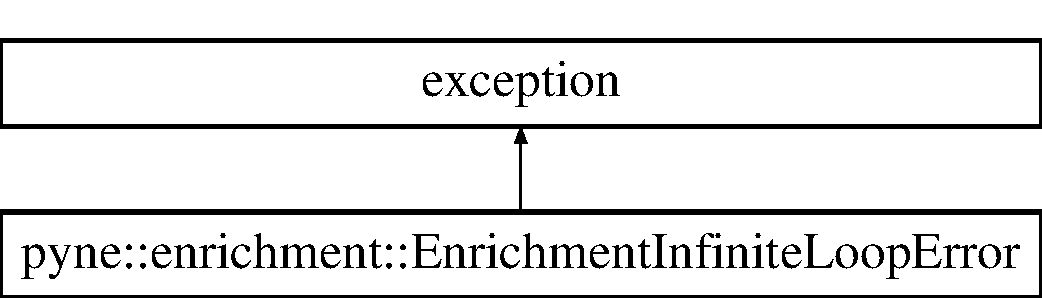
\includegraphics[height=2.000000cm]{classpyne_1_1enrichment_1_1_enrichment_infinite_loop_error}
\end{center}
\end{figure}


\subsection{Detailed Description}
Custom exception for when an enrichment solver has entered an infinite loop. 

The documentation for this class was generated from the following file\+:\begin{DoxyCompactItemize}
\item 
/home/ubuntu/\+Documents/pyne.\+github.\+com/src/\hyperlink{enrichment_8h}{enrichment.\+h}\end{DoxyCompactItemize}

\hypertarget{classpyne_1_1enrichment_1_1_enrichment_iteration_limit}{}\section{pyne\+:\+:enrichment\+:\+:Enrichment\+Iteration\+Limit Class Reference}
\label{classpyne_1_1enrichment_1_1_enrichment_iteration_limit}\index{pyne\+::enrichment\+::\+Enrichment\+Iteration\+Limit@{pyne\+::enrichment\+::\+Enrichment\+Iteration\+Limit}}


{\ttfamily \#include $<$enrichment.\+h$>$}

Inheritance diagram for pyne\+:\+:enrichment\+:\+:Enrichment\+Iteration\+Limit\+:\begin{figure}[H]
\begin{center}
\leavevmode
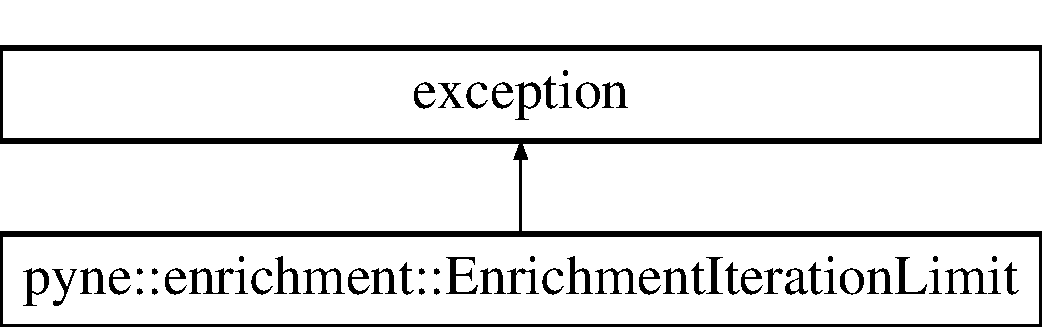
\includegraphics[height=2.000000cm]{classpyne_1_1enrichment_1_1_enrichment_iteration_limit}
\end{center}
\end{figure}


\subsection{Detailed Description}
Custom exception for when an enrichment solver has reached its maximum number of iterations. 

The documentation for this class was generated from the following file\+:\begin{DoxyCompactItemize}
\item 
/home/lucas/opt/gcc-\/6/pyne-\/dev/pyne/src/\hyperlink{enrichment_8h}{enrichment.\+h}\end{DoxyCompactItemize}

\hypertarget{classpyne_1_1enrichment_1_1_enrichment_iteration_na_n}{}\section{pyne\+:\+:enrichment\+:\+:Enrichment\+Iteration\+NaN Class Reference}
\label{classpyne_1_1enrichment_1_1_enrichment_iteration_na_n}\index{pyne\+::enrichment\+::\+Enrichment\+Iteration\+NaN@{pyne\+::enrichment\+::\+Enrichment\+Iteration\+NaN}}


Custom exception for when an enrichment solver iteration has produced a NaN.  




{\ttfamily \#include $<$enrichment.\+h$>$}

Inheritance diagram for pyne\+:\+:enrichment\+:\+:Enrichment\+Iteration\+NaN\+:\begin{figure}[H]
\begin{center}
\leavevmode
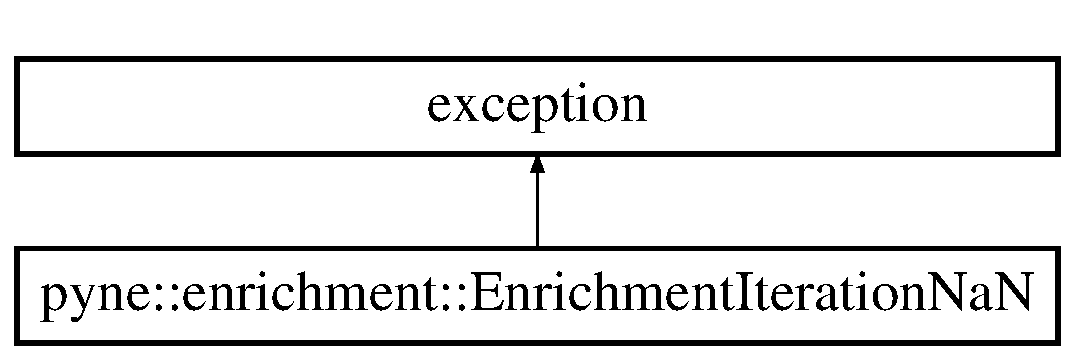
\includegraphics[height=2.000000cm]{classpyne_1_1enrichment_1_1_enrichment_iteration_na_n}
\end{center}
\end{figure}


\subsection{Detailed Description}
Custom exception for when an enrichment solver iteration has produced a NaN. 

The documentation for this class was generated from the following file\+:\begin{DoxyCompactItemize}
\item 
/home/ubuntu/\+Desktop/new/pyne.\+github.\+com/src/\hyperlink{enrichment_8h}{enrichment.\+h}\end{DoxyCompactItemize}

\hypertarget{classpyne_1_1_file_not_found}{}\section{pyne\+:\+:File\+Not\+Found Class Reference}
\label{classpyne_1_1_file_not_found}\index{pyne\+::\+File\+Not\+Found@{pyne\+::\+File\+Not\+Found}}


{\ttfamily \#include $<$utils.\+h$>$}

Inheritance diagram for pyne\+:\+:File\+Not\+Found\+:\begin{figure}[H]
\begin{center}
\leavevmode
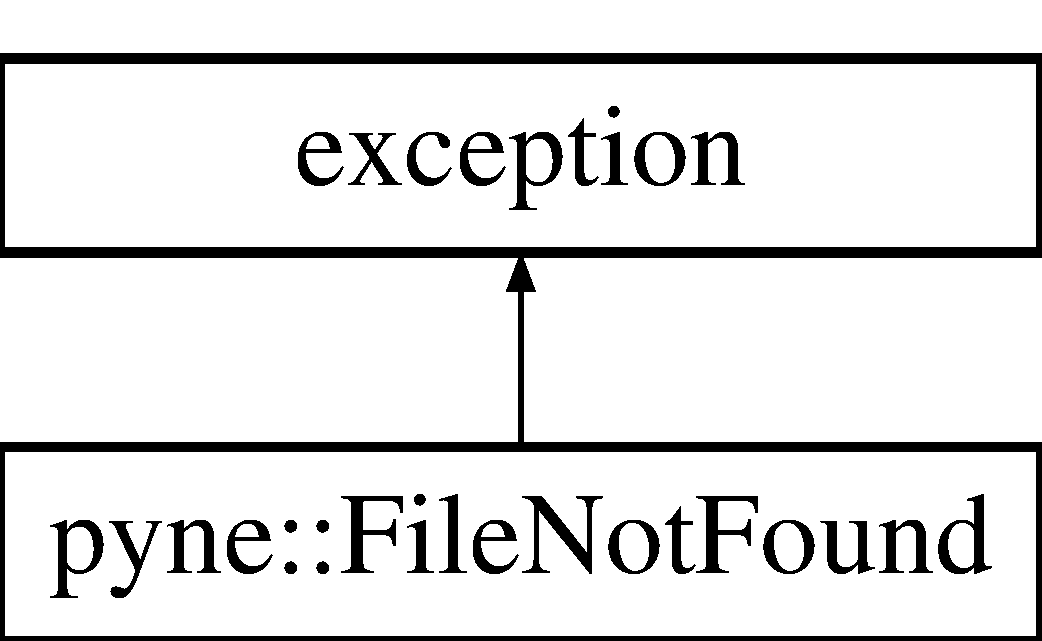
\includegraphics[height=2.000000cm]{classpyne_1_1_file_not_found}
\end{center}
\end{figure}
\subsection*{Public Member Functions}
\begin{DoxyCompactItemize}
\item 
\hyperlink{classpyne_1_1_file_not_found_aaae1bdf04df2b68377ae453929c8eb56}{File\+Not\+Found} ()\hypertarget{classpyne_1_1_file_not_found_aaae1bdf04df2b68377ae453929c8eb56}{}\label{classpyne_1_1_file_not_found_aaae1bdf04df2b68377ae453929c8eb56}

\begin{DoxyCompactList}\small\item\em default constructor \end{DoxyCompactList}\item 
\hyperlink{classpyne_1_1_file_not_found_abc00e9c8711bb1b1bb2dc1dfd3a98745}{$\sim$\+File\+Not\+Found} ()  throw ()\hypertarget{classpyne_1_1_file_not_found_abc00e9c8711bb1b1bb2dc1dfd3a98745}{}\label{classpyne_1_1_file_not_found_abc00e9c8711bb1b1bb2dc1dfd3a98745}

\begin{DoxyCompactList}\small\item\em default destructor \end{DoxyCompactList}\item 
\hyperlink{classpyne_1_1_file_not_found_a4d766115c01634b77aebe42269f9aead}{File\+Not\+Found} (std\+::string fname)\hypertarget{classpyne_1_1_file_not_found_a4d766115c01634b77aebe42269f9aead}{}\label{classpyne_1_1_file_not_found_a4d766115c01634b77aebe42269f9aead}

\begin{DoxyCompactList}\small\item\em constructor with the filename {\itshape fname}. \end{DoxyCompactList}\item 
virtual const char $\ast$ \hyperlink{classpyne_1_1_file_not_found_a55d410139d5853e8988d073637845cbd}{what} () const   throw ()\hypertarget{classpyne_1_1_file_not_found_a55d410139d5853e8988d073637845cbd}{}\label{classpyne_1_1_file_not_found_a55d410139d5853e8988d073637845cbd}

\begin{DoxyCompactList}\small\item\em Creates a helpful error message. \end{DoxyCompactList}\end{DoxyCompactItemize}


\subsection{Detailed Description}
Custom exception to be thrown in the event that a required file is not able to be found. 

The documentation for this class was generated from the following file\+:\begin{DoxyCompactItemize}
\item 
/home/ubuntu/\+Desktop/new/pyne.\+github.\+com/src/utils.\+h\end{DoxyCompactItemize}

\hypertarget{classh5wrap_1_1_file_not_h_d_f5}{}\section{h5wrap\+:\+:File\+Not\+H\+D\+F5 Class Reference}
\label{classh5wrap_1_1_file_not_h_d_f5}\index{h5wrap\+::\+File\+Not\+H\+D\+F5@{h5wrap\+::\+File\+Not\+H\+D\+F5}}


Custom exception for when an existing file is not in a valid H\+D\+F5 format.  




{\ttfamily \#include $<$h5wrap.\+h$>$}

Inheritance diagram for h5wrap\+:\+:File\+Not\+H\+D\+F5\+:\begin{figure}[H]
\begin{center}
\leavevmode
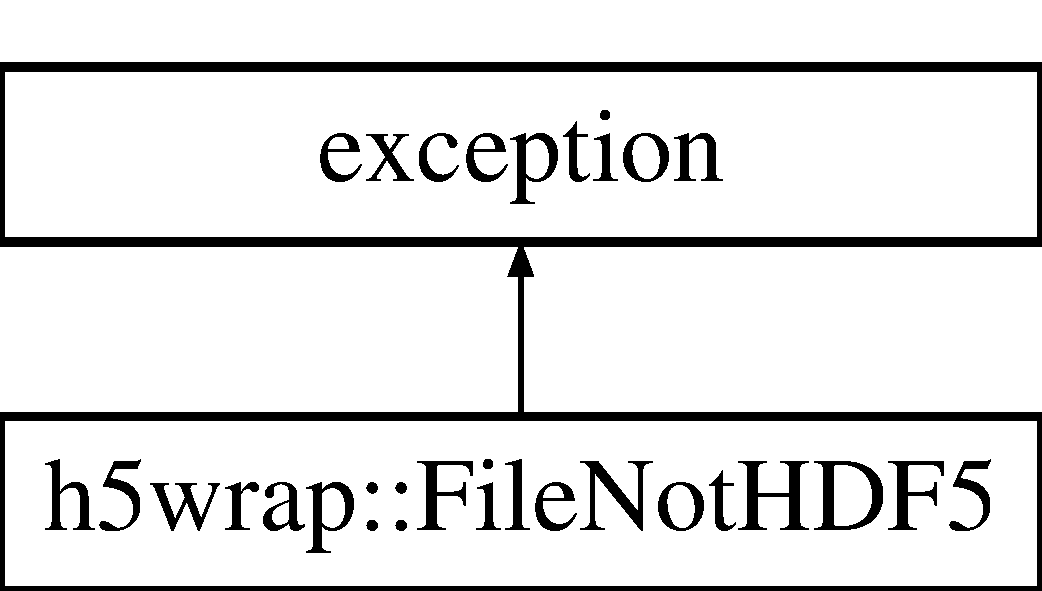
\includegraphics[height=2.000000cm]{classh5wrap_1_1_file_not_h_d_f5}
\end{center}
\end{figure}
\subsection*{Public Member Functions}
\begin{DoxyCompactItemize}
\item 
\hyperlink{classh5wrap_1_1_file_not_h_d_f5_a3fa40cb39abaa241e80ee97a13e69815}{File\+Not\+H\+D\+F5} ()\hypertarget{classh5wrap_1_1_file_not_h_d_f5_a3fa40cb39abaa241e80ee97a13e69815}{}\label{classh5wrap_1_1_file_not_h_d_f5_a3fa40cb39abaa241e80ee97a13e69815}

\begin{DoxyCompactList}\small\item\em default constructor \end{DoxyCompactList}\item 
\hyperlink{classh5wrap_1_1_file_not_h_d_f5_a55276b2bc97da82f25a0718327b00742}{$\sim$\+File\+Not\+H\+D\+F5} ()  throw ()\hypertarget{classh5wrap_1_1_file_not_h_d_f5_a55276b2bc97da82f25a0718327b00742}{}\label{classh5wrap_1_1_file_not_h_d_f5_a55276b2bc97da82f25a0718327b00742}

\begin{DoxyCompactList}\small\item\em default destructor \end{DoxyCompactList}\item 
\hyperlink{classh5wrap_1_1_file_not_h_d_f5_ac6f9e6588f3a55f26fe6cd13ab75425b}{File\+Not\+H\+D\+F5} (std\+::string fname)\hypertarget{classh5wrap_1_1_file_not_h_d_f5_ac6f9e6588f3a55f26fe6cd13ab75425b}{}\label{classh5wrap_1_1_file_not_h_d_f5_ac6f9e6588f3a55f26fe6cd13ab75425b}

\begin{DoxyCompactList}\small\item\em constructor with the filename \end{DoxyCompactList}\item 
virtual const char $\ast$ \hyperlink{classh5wrap_1_1_file_not_h_d_f5_afce2273e3c8d54802598bdc30cdedec2}{what} () const   throw ()\hypertarget{classh5wrap_1_1_file_not_h_d_f5_afce2273e3c8d54802598bdc30cdedec2}{}\label{classh5wrap_1_1_file_not_h_d_f5_afce2273e3c8d54802598bdc30cdedec2}

\begin{DoxyCompactList}\small\item\em helpful error message that includes the filename \end{DoxyCompactList}\end{DoxyCompactItemize}


\subsection{Detailed Description}
Custom exception for when an existing file is not in a valid H\+D\+F5 format. 

The documentation for this class was generated from the following file\+:\begin{DoxyCompactItemize}
\item 
/home/ubuntu/\+Desktop/new/pyne.\+github.\+com/src/\hyperlink{h5wrap_8h}{h5wrap.\+h}\end{DoxyCompactItemize}

\hypertarget{structpyne_1_1gamma}{}\section{pyne\+:\+:gamma Struct Reference}
\label{structpyne_1_1gamma}\index{pyne\+::gamma@{pyne\+::gamma}}


a struct matching the \textquotesingle{}/decay/gammas\textquotesingle{} table in nuc\+\_\+data.\+h5.  




{\ttfamily \#include $<$data.\+h$>$}

\subsection*{Public Attributes}
\begin{DoxyCompactItemize}
\item 
int \hyperlink{structpyne_1_1gamma_a1c5b7ef9f75c628193a0872c9ae172e4}{from\+\_\+nuc}\hypertarget{structpyne_1_1gamma_a1c5b7ef9f75c628193a0872c9ae172e4}{}\label{structpyne_1_1gamma_a1c5b7ef9f75c628193a0872c9ae172e4}

\begin{DoxyCompactList}\small\item\em state id of starting level \end{DoxyCompactList}\item 
int \hyperlink{structpyne_1_1gamma_af9ed390289a667c82464c859dbccb0a4}{to\+\_\+nuc}\hypertarget{structpyne_1_1gamma_af9ed390289a667c82464c859dbccb0a4}{}\label{structpyne_1_1gamma_af9ed390289a667c82464c859dbccb0a4}

\begin{DoxyCompactList}\small\item\em state id of final level \end{DoxyCompactList}\item 
int \hyperlink{structpyne_1_1gamma_a947386fa2557f57cc14f79d6904185bd}{parent\+\_\+nuc}\hypertarget{structpyne_1_1gamma_a947386fa2557f57cc14f79d6904185bd}{}\label{structpyne_1_1gamma_a947386fa2557f57cc14f79d6904185bd}

\begin{DoxyCompactList}\small\item\em state id of the primary decaying nucleus \end{DoxyCompactList}\item 
int \hyperlink{structpyne_1_1gamma_a99fcb3ccd78db851f7104ff3ab59048d}{child\+\_\+nuc}\hypertarget{structpyne_1_1gamma_a99fcb3ccd78db851f7104ff3ab59048d}{}\label{structpyne_1_1gamma_a99fcb3ccd78db851f7104ff3ab59048d}

\begin{DoxyCompactList}\small\item\em stateless id of the child nucleus \end{DoxyCompactList}\item 
double \hyperlink{structpyne_1_1gamma_a82e14610a750a9c31c6976c2685c223f}{energy}\hypertarget{structpyne_1_1gamma_a82e14610a750a9c31c6976c2685c223f}{}\label{structpyne_1_1gamma_a82e14610a750a9c31c6976c2685c223f}

\begin{DoxyCompactList}\small\item\em energy of the photon \mbox{[}keV\mbox{]} \end{DoxyCompactList}\item 
double \hyperlink{structpyne_1_1gamma_a9682d9995810db3b59d27138c24e223a}{energy\+\_\+err}\hypertarget{structpyne_1_1gamma_a9682d9995810db3b59d27138c24e223a}{}\label{structpyne_1_1gamma_a9682d9995810db3b59d27138c24e223a}

\begin{DoxyCompactList}\small\item\em energy error of the photon \mbox{[}keV\mbox{]} \end{DoxyCompactList}\item 
double \hyperlink{structpyne_1_1gamma_a5d7ca7cc0667ebc41b8f046739c0dc1b}{photon\+\_\+intensity}\hypertarget{structpyne_1_1gamma_a5d7ca7cc0667ebc41b8f046739c0dc1b}{}\label{structpyne_1_1gamma_a5d7ca7cc0667ebc41b8f046739c0dc1b}

\begin{DoxyCompactList}\small\item\em photon intensity \end{DoxyCompactList}\item 
double \hyperlink{structpyne_1_1gamma_a38f1045e9df163a740c657ca6cac490b}{photon\+\_\+intensity\+\_\+err}\hypertarget{structpyne_1_1gamma_a38f1045e9df163a740c657ca6cac490b}{}\label{structpyne_1_1gamma_a38f1045e9df163a740c657ca6cac490b}

\begin{DoxyCompactList}\small\item\em photon intensity error \end{DoxyCompactList}\item 
double \hyperlink{structpyne_1_1gamma_a6d347a0a5cfcf0765476d618b2faa71f}{conv\+\_\+intensity}\hypertarget{structpyne_1_1gamma_a6d347a0a5cfcf0765476d618b2faa71f}{}\label{structpyne_1_1gamma_a6d347a0a5cfcf0765476d618b2faa71f}

\begin{DoxyCompactList}\small\item\em conversion intensity \end{DoxyCompactList}\item 
double \hyperlink{structpyne_1_1gamma_a48c4d772b76640e6cd77805278241657}{conv\+\_\+intensity\+\_\+err}\hypertarget{structpyne_1_1gamma_a48c4d772b76640e6cd77805278241657}{}\label{structpyne_1_1gamma_a48c4d772b76640e6cd77805278241657}

\begin{DoxyCompactList}\small\item\em conversion intensity error \end{DoxyCompactList}\item 
double \hyperlink{structpyne_1_1gamma_a5d409f6a09142b6cc871158cff7d5fe7}{total\+\_\+intensity}\hypertarget{structpyne_1_1gamma_a5d409f6a09142b6cc871158cff7d5fe7}{}\label{structpyne_1_1gamma_a5d409f6a09142b6cc871158cff7d5fe7}

\begin{DoxyCompactList}\small\item\em total decay intensity \end{DoxyCompactList}\item 
double \hyperlink{structpyne_1_1gamma_a8c626cfbe36afddfadf664f2aff19f2f}{total\+\_\+intensity\+\_\+err}\hypertarget{structpyne_1_1gamma_a8c626cfbe36afddfadf664f2aff19f2f}{}\label{structpyne_1_1gamma_a8c626cfbe36afddfadf664f2aff19f2f}

\begin{DoxyCompactList}\small\item\em total decay intensity error \end{DoxyCompactList}\item 
double \hyperlink{structpyne_1_1gamma_a9b4256e35bdd191c7a6c27835642e353}{k\+\_\+conv\+\_\+e}\hypertarget{structpyne_1_1gamma_a9b4256e35bdd191c7a6c27835642e353}{}\label{structpyne_1_1gamma_a9b4256e35bdd191c7a6c27835642e353}

\begin{DoxyCompactList}\small\item\em k conversion electron fraction \end{DoxyCompactList}\item 
double \hyperlink{structpyne_1_1gamma_a9fbb2fdf8a1c5b7430afa34237509abe}{l\+\_\+conv\+\_\+e}\hypertarget{structpyne_1_1gamma_a9fbb2fdf8a1c5b7430afa34237509abe}{}\label{structpyne_1_1gamma_a9fbb2fdf8a1c5b7430afa34237509abe}

\begin{DoxyCompactList}\small\item\em l conversion electron fraction \end{DoxyCompactList}\item 
double \hyperlink{structpyne_1_1gamma_a6c664717050818947e2e79d75e914c41}{m\+\_\+conv\+\_\+e}\hypertarget{structpyne_1_1gamma_a6c664717050818947e2e79d75e914c41}{}\label{structpyne_1_1gamma_a6c664717050818947e2e79d75e914c41}

\begin{DoxyCompactList}\small\item\em m conversion electron fraction \end{DoxyCompactList}\end{DoxyCompactItemize}


\subsection{Detailed Description}
a struct matching the \textquotesingle{}/decay/gammas\textquotesingle{} table in nuc\+\_\+data.\+h5. 

The documentation for this struct was generated from the following file\+:\begin{DoxyCompactItemize}
\item 
/home/ubuntu/\+Documents/pyne.\+github.\+com/src/\hyperlink{data_8h}{data.\+h}\end{DoxyCompactItemize}

\hypertarget{classh5wrap_1_1_group_not_found}{}\section{h5wrap\+:\+:Group\+Not\+Found Class Reference}
\label{classh5wrap_1_1_group_not_found}\index{h5wrap\+::\+Group\+Not\+Found@{h5wrap\+::\+Group\+Not\+Found}}


Custom exception for when a group cannot be found in an H\+D\+F5 file.  




{\ttfamily \#include $<$h5wrap.\+h$>$}

Inheritance diagram for h5wrap\+:\+:Group\+Not\+Found\+:\begin{figure}[H]
\begin{center}
\leavevmode
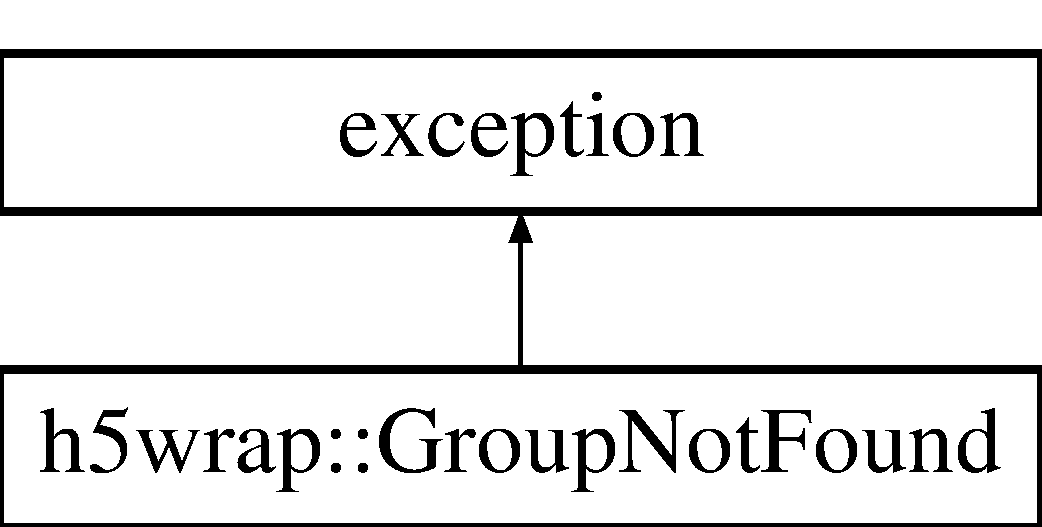
\includegraphics[height=2.000000cm]{classh5wrap_1_1_group_not_found}
\end{center}
\end{figure}
\subsection*{Public Member Functions}
\begin{DoxyCompactItemize}
\item 
\hyperlink{classh5wrap_1_1_group_not_found_accc7d7bea9e86968335a46ee39d7d543}{Group\+Not\+Found} ()\hypertarget{classh5wrap_1_1_group_not_found_accc7d7bea9e86968335a46ee39d7d543}{}\label{classh5wrap_1_1_group_not_found_accc7d7bea9e86968335a46ee39d7d543}

\begin{DoxyCompactList}\small\item\em default constructor \end{DoxyCompactList}\item 
\hyperlink{classh5wrap_1_1_group_not_found_a79dea7d1d5e3ffd7a7e83b4a2636398a}{$\sim$\+Group\+Not\+Found} ()  throw ()\hypertarget{classh5wrap_1_1_group_not_found_a79dea7d1d5e3ffd7a7e83b4a2636398a}{}\label{classh5wrap_1_1_group_not_found_a79dea7d1d5e3ffd7a7e83b4a2636398a}

\begin{DoxyCompactList}\small\item\em default destructor \end{DoxyCompactList}\item 
\hyperlink{classh5wrap_1_1_group_not_found_a74f7e8f6efcf33503f5fec62eead40c3}{Group\+Not\+Found} (std\+::string fname, std\+::string gname)\hypertarget{classh5wrap_1_1_group_not_found_a74f7e8f6efcf33503f5fec62eead40c3}{}\label{classh5wrap_1_1_group_not_found_a74f7e8f6efcf33503f5fec62eead40c3}

\begin{DoxyCompactList}\small\item\em constructor with the filename and the groupname \end{DoxyCompactList}\item 
virtual const char $\ast$ \hyperlink{classh5wrap_1_1_group_not_found_a76766dc5fda0a07564379db454df87d0}{what} () const   throw ()\hypertarget{classh5wrap_1_1_group_not_found_a76766dc5fda0a07564379db454df87d0}{}\label{classh5wrap_1_1_group_not_found_a76766dc5fda0a07564379db454df87d0}

\begin{DoxyCompactList}\small\item\em helpful error message that includes the filename and the groupname \end{DoxyCompactList}\end{DoxyCompactItemize}


\subsection{Detailed Description}
Custom exception for when a group cannot be found in an H\+D\+F5 file. 

The documentation for this class was generated from the following file\+:\begin{DoxyCompactItemize}
\item 
/home/lucas/opt/gcc-\/6/pyne-\/dev/pyne/src/\hyperlink{h5wrap_8h}{h5wrap.\+h}\end{DoxyCompactItemize}

\hypertarget{classh5wrap_1_1_h_d_f5_bounds_error}{}\section{h5wrap\+:\+:H\+D\+F5\+Bounds\+Error Class Reference}
\label{classh5wrap_1_1_h_d_f5_bounds_error}\index{h5wrap\+::\+H\+D\+F5\+Bounds\+Error@{h5wrap\+::\+H\+D\+F5\+Bounds\+Error}}


Custom exception for H\+D\+F5 indexing errors.  




{\ttfamily \#include $<$h5wrap.\+h$>$}

Inheritance diagram for h5wrap\+:\+:H\+D\+F5\+Bounds\+Error\+:\begin{figure}[H]
\begin{center}
\leavevmode
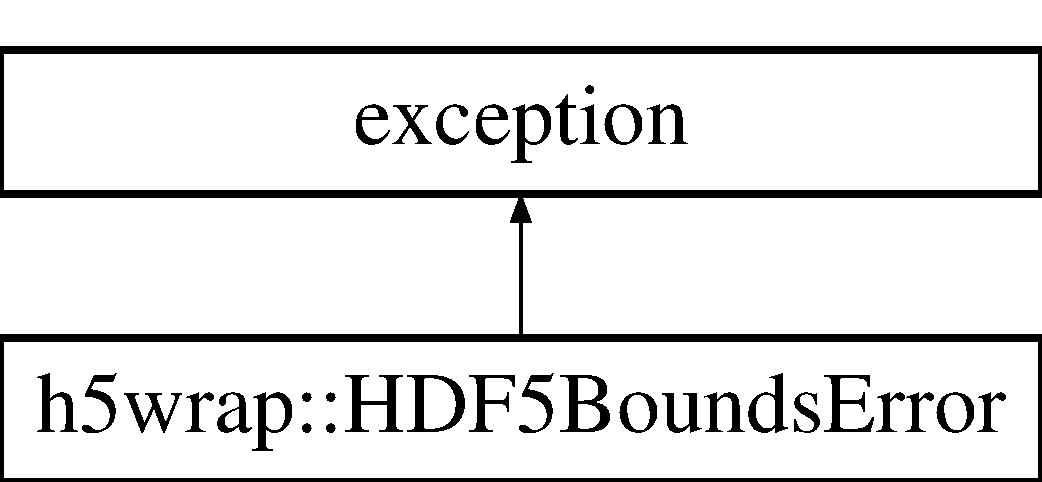
\includegraphics[height=2.000000cm]{classh5wrap_1_1_h_d_f5_bounds_error}
\end{center}
\end{figure}


\subsection{Detailed Description}
Custom exception for H\+D\+F5 indexing errors. 

The documentation for this class was generated from the following file\+:\begin{DoxyCompactItemize}
\item 
/home/ubuntu/\+Documents/pyne.\+github.\+com/src/\hyperlink{h5wrap_8h}{h5wrap.\+h}\end{DoxyCompactItemize}

\hypertarget{classh5wrap_1_1_homogenous_type_table}{}\section{h5wrap\+:\+:Homogenous\+Type\+Table$<$ T $>$ Class Template Reference}
\label{classh5wrap_1_1_homogenous_type_table}\index{h5wrap\+::\+Homogenous\+Type\+Table$<$ T $>$@{h5wrap\+::\+Homogenous\+Type\+Table$<$ T $>$}}


{\ttfamily \#include $<$h5wrap.\+h$>$}

\subsection*{Public Member Functions}
\begin{DoxyCompactItemize}
\item 
\hyperlink{classh5wrap_1_1_homogenous_type_table_a4abe000d3595d0ff78354bc5131b1ca7}{Homogenous\+Type\+Table} ()\hypertarget{classh5wrap_1_1_homogenous_type_table_a4abe000d3595d0ff78354bc5131b1ca7}{}\label{classh5wrap_1_1_homogenous_type_table_a4abe000d3595d0ff78354bc5131b1ca7}

\begin{DoxyCompactList}\small\item\em default constructor \end{DoxyCompactList}\item 
\hyperlink{classh5wrap_1_1_homogenous_type_table_aa339bef26857f755e42035d4e054d7c7}{$\sim$\+Homogenous\+Type\+Table} ()\hypertarget{classh5wrap_1_1_homogenous_type_table_aa339bef26857f755e42035d4e054d7c7}{}\label{classh5wrap_1_1_homogenous_type_table_aa339bef26857f755e42035d4e054d7c7}

\begin{DoxyCompactList}\small\item\em default destructor \end{DoxyCompactList}\item 
\hyperlink{classh5wrap_1_1_homogenous_type_table_a2fd7306656d5a16b4a44b50a9271eab3}{Homogenous\+Type\+Table} (hid\+\_\+t h5file, std\+::string data\+\_\+path, hid\+\_\+t dtype=H5\+T\+\_\+\+N\+A\+T\+I\+V\+E\+\_\+\+D\+O\+U\+B\+LE)
\item 
std\+::vector$<$ T $>$ \hyperlink{classh5wrap_1_1_homogenous_type_table_a961e0edb817f203b00367202d3c278b4}{operator\mbox{[}$\,$\mbox{]}} (std\+::string col\+\_\+name)\hypertarget{classh5wrap_1_1_homogenous_type_table_a961e0edb817f203b00367202d3c278b4}{}\label{classh5wrap_1_1_homogenous_type_table_a961e0edb817f203b00367202d3c278b4}

\begin{DoxyCompactList}\small\item\em index into the table by column name (string) \end{DoxyCompactList}\item 
std\+::map$<$ std\+::string, T $>$ \hyperlink{classh5wrap_1_1_homogenous_type_table_a777f6bdc03111b5a7d8fde59e184e26c}{operator\mbox{[}$\,$\mbox{]}} (int m)\hypertarget{classh5wrap_1_1_homogenous_type_table_a777f6bdc03111b5a7d8fde59e184e26c}{}\label{classh5wrap_1_1_homogenous_type_table_a777f6bdc03111b5a7d8fde59e184e26c}

\begin{DoxyCompactList}\small\item\em index into the table by row \end{DoxyCompactList}\end{DoxyCompactItemize}
\subsection*{Public Attributes}
\begin{DoxyCompactItemize}
\item 
std\+::string \hyperlink{classh5wrap_1_1_homogenous_type_table_a6da460e4b94719f9ff5fe0d17e8859d7}{path}\hypertarget{classh5wrap_1_1_homogenous_type_table_a6da460e4b94719f9ff5fe0d17e8859d7}{}\label{classh5wrap_1_1_homogenous_type_table_a6da460e4b94719f9ff5fe0d17e8859d7}

\begin{DoxyCompactList}\small\item\em path in file to the data \end{DoxyCompactList}\item 
int \hyperlink{classh5wrap_1_1_homogenous_type_table_ab0e03ddbee134e775ea6fa389897fc8b}{shape} \mbox{[}2\mbox{]}\hypertarget{classh5wrap_1_1_homogenous_type_table_ab0e03ddbee134e775ea6fa389897fc8b}{}\label{classh5wrap_1_1_homogenous_type_table_ab0e03ddbee134e775ea6fa389897fc8b}

\begin{DoxyCompactList}\small\item\em table shape, rows x columns. \end{DoxyCompactList}\item 
std\+::vector$<$ std\+::string $>$ \hyperlink{classh5wrap_1_1_homogenous_type_table_a8b60fa54475f44bea26caab0137d8507}{cols}
\item 
std\+::map$<$ std\+::string, std\+::vector$<$ T $>$ $>$ \hyperlink{classh5wrap_1_1_homogenous_type_table_a06c1889b5469abf303923b17b78a381b}{data}\hypertarget{classh5wrap_1_1_homogenous_type_table_a06c1889b5469abf303923b17b78a381b}{}\label{classh5wrap_1_1_homogenous_type_table_a06c1889b5469abf303923b17b78a381b}

\begin{DoxyCompactList}\small\item\em mapping from column names to column data \end{DoxyCompactList}\end{DoxyCompactItemize}


\subsection{Detailed Description}
\subsubsection*{template$<$typename T$>$\\*
class h5wrap\+::\+Homogenous\+Type\+Table$<$ T $>$}

A class representing a high-\/level table contruct whose columns all have the same type {\itshape T} in C/\+C++ (and the analogous type in H\+D\+F5). 

\subsection{Constructor \& Destructor Documentation}
\index{h5wrap\+::\+Homogenous\+Type\+Table@{h5wrap\+::\+Homogenous\+Type\+Table}!Homogenous\+Type\+Table@{Homogenous\+Type\+Table}}
\index{Homogenous\+Type\+Table@{Homogenous\+Type\+Table}!h5wrap\+::\+Homogenous\+Type\+Table@{h5wrap\+::\+Homogenous\+Type\+Table}}
\subsubsection[{\texorpdfstring{Homogenous\+Type\+Table(hid\+\_\+t h5file, std\+::string data\+\_\+path, hid\+\_\+t dtype=\+H5\+T\+\_\+\+N\+A\+T\+I\+V\+E\+\_\+\+D\+O\+U\+B\+L\+E)}{HomogenousTypeTable(hid_t h5file, std::string data_path, hid_t dtype=H5T_NATIVE_DOUBLE)}}]{\setlength{\rightskip}{0pt plus 5cm}template$<$typename T $>$ {\bf h5wrap\+::\+Homogenous\+Type\+Table}$<$ T $>$\+::{\bf Homogenous\+Type\+Table} (
\begin{DoxyParamCaption}
\item[{hid\+\_\+t}]{h5file, }
\item[{std\+::string}]{data\+\_\+path, }
\item[{hid\+\_\+t}]{dtype = {\ttfamily H5T\+\_\+NATIVE\+\_\+DOUBLE}}
\end{DoxyParamCaption}
)\hspace{0.3cm}{\ttfamily [inline]}}\hypertarget{classh5wrap_1_1_homogenous_type_table_a2fd7306656d5a16b4a44b50a9271eab3}{}\label{classh5wrap_1_1_homogenous_type_table_a2fd7306656d5a16b4a44b50a9271eab3}
Constructor to load in data upon initialization. {\itshape T} should roughly match {\itshape dtype}. 
\begin{DoxyParams}{Parameters}
{\em h5file} & H\+D\+F5 file id for an open file. \\
\hline
{\em data\+\_\+path} & path to the data in the open file. \\
\hline
{\em dtype} & H\+D\+F5 data type for the data set at {\itshape data\+\_\+path}. \\
\hline
\end{DoxyParams}


\subsection{Member Data Documentation}
\index{h5wrap\+::\+Homogenous\+Type\+Table@{h5wrap\+::\+Homogenous\+Type\+Table}!cols@{cols}}
\index{cols@{cols}!h5wrap\+::\+Homogenous\+Type\+Table@{h5wrap\+::\+Homogenous\+Type\+Table}}
\subsubsection[{\texorpdfstring{cols}{cols}}]{\setlength{\rightskip}{0pt plus 5cm}template$<$typename T $>$ std\+::vector$<$std\+::string$>$ {\bf h5wrap\+::\+Homogenous\+Type\+Table}$<$ T $>$\+::cols}\hypertarget{classh5wrap_1_1_homogenous_type_table_a8b60fa54475f44bea26caab0137d8507}{}\label{classh5wrap_1_1_homogenous_type_table_a8b60fa54475f44bea26caab0137d8507}
column names 

The documentation for this class was generated from the following file\+:\begin{DoxyCompactItemize}
\item 
/home/ubuntu/\+Desktop/new/pyne.\+github.\+com/src/\hyperlink{h5wrap_8h}{h5wrap.\+h}\end{DoxyCompactItemize}

\hypertarget{classpyne_1_1nucname_1_1_indeterminate_nuclide_form}{}\section{pyne\+:\+:nucname\+:\+:Indeterminate\+Nuclide\+Form Class Reference}
\label{classpyne_1_1nucname_1_1_indeterminate_nuclide_form}\index{pyne\+::nucname\+::\+Indeterminate\+Nuclide\+Form@{pyne\+::nucname\+::\+Indeterminate\+Nuclide\+Form}}


{\ttfamily \#include $<$nucname.\+h$>$}

Inheritance diagram for pyne\+:\+:nucname\+:\+:Indeterminate\+Nuclide\+Form\+:\begin{figure}[H]
\begin{center}
\leavevmode
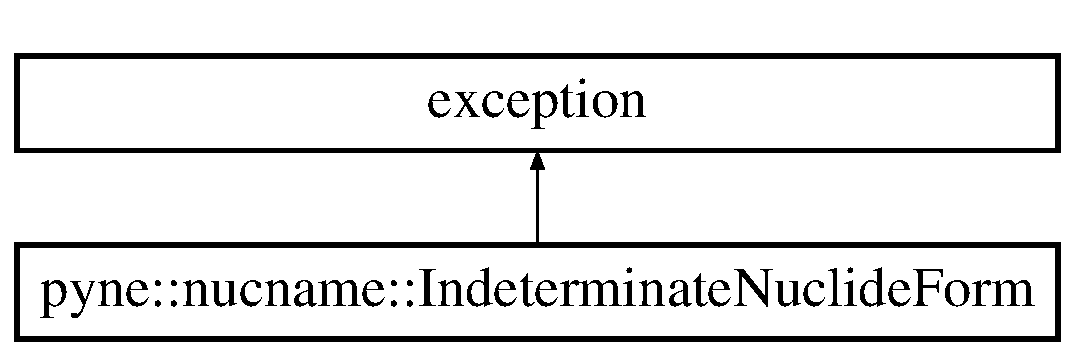
\includegraphics[height=2.000000cm]{classpyne_1_1nucname_1_1_indeterminate_nuclide_form}
\end{center}
\end{figure}
\subsection*{Public Member Functions}
\begin{DoxyCompactItemize}
\item 
\hyperlink{classpyne_1_1nucname_1_1_indeterminate_nuclide_form_aee3a250200624d6f4ab5935fd1e13d21}{Indeterminate\+Nuclide\+Form} ()\hypertarget{classpyne_1_1nucname_1_1_indeterminate_nuclide_form_aee3a250200624d6f4ab5935fd1e13d21}{}\label{classpyne_1_1nucname_1_1_indeterminate_nuclide_form_aee3a250200624d6f4ab5935fd1e13d21}

\begin{DoxyCompactList}\small\item\em default constructor \end{DoxyCompactList}\item 
\hyperlink{classpyne_1_1nucname_1_1_indeterminate_nuclide_form_afc4bbaae82a451dcbf3a85b62ab8de0e}{$\sim$\+Indeterminate\+Nuclide\+Form} ()  throw ()\hypertarget{classpyne_1_1nucname_1_1_indeterminate_nuclide_form_afc4bbaae82a451dcbf3a85b62ab8de0e}{}\label{classpyne_1_1nucname_1_1_indeterminate_nuclide_form_afc4bbaae82a451dcbf3a85b62ab8de0e}

\begin{DoxyCompactList}\small\item\em default destuctor \end{DoxyCompactList}\item 
\hyperlink{classpyne_1_1nucname_1_1_indeterminate_nuclide_form_a74d77801a214b679461eaf5dfbf7ab02}{Indeterminate\+Nuclide\+Form} (std\+::string wasptr, std\+::string nowptr)
\item 
\hyperlink{classpyne_1_1nucname_1_1_indeterminate_nuclide_form_a93724a9906be5a73b43b09ecdfed872d}{Indeterminate\+Nuclide\+Form} (std\+::string wasptr, int nowptr)
\item 
\hyperlink{classpyne_1_1nucname_1_1_indeterminate_nuclide_form_a3c9c6d0c859f3344fbb78b4259733678}{Indeterminate\+Nuclide\+Form} (int wasptr, std\+::string nowptr)
\item 
\hyperlink{classpyne_1_1nucname_1_1_indeterminate_nuclide_form_a565a1ca748bf437b18eee4834f65bf19}{Indeterminate\+Nuclide\+Form} (int wasptr, int nowptr)
\item 
virtual const char $\ast$ \hyperlink{classpyne_1_1nucname_1_1_indeterminate_nuclide_form_a9103205a7bd38dec5118e84508ed4bdb}{what} () const   throw ()
\end{DoxyCompactItemize}


\subsection{Detailed Description}
Custom expection for declaring that a value represents one or more nuclides in one or more namig conventions 

\subsection{Constructor \& Destructor Documentation}
\index{pyne\+::nucname\+::\+Indeterminate\+Nuclide\+Form@{pyne\+::nucname\+::\+Indeterminate\+Nuclide\+Form}!Indeterminate\+Nuclide\+Form@{Indeterminate\+Nuclide\+Form}}
\index{Indeterminate\+Nuclide\+Form@{Indeterminate\+Nuclide\+Form}!pyne\+::nucname\+::\+Indeterminate\+Nuclide\+Form@{pyne\+::nucname\+::\+Indeterminate\+Nuclide\+Form}}
\subsubsection[{\texorpdfstring{Indeterminate\+Nuclide\+Form(std\+::string wasptr, std\+::string nowptr)}{IndeterminateNuclideForm(std::string wasptr, std::string nowptr)}}]{\setlength{\rightskip}{0pt plus 5cm}pyne\+::nucname\+::\+Indeterminate\+Nuclide\+Form\+::\+Indeterminate\+Nuclide\+Form (
\begin{DoxyParamCaption}
\item[{std\+::string}]{wasptr, }
\item[{std\+::string}]{nowptr}
\end{DoxyParamCaption}
)\hspace{0.3cm}{\ttfamily [inline]}}\hypertarget{classpyne_1_1nucname_1_1_indeterminate_nuclide_form_a74d77801a214b679461eaf5dfbf7ab02}{}\label{classpyne_1_1nucname_1_1_indeterminate_nuclide_form_a74d77801a214b679461eaf5dfbf7ab02}
Constructor given previous and current state of nulide name 
\begin{DoxyParams}{Parameters}
{\em wasptr} & Previous state, typically user input. \\
\hline
{\em nowptr} & Current state, as far as Py\+NE could get. \\
\hline
\end{DoxyParams}
\index{pyne\+::nucname\+::\+Indeterminate\+Nuclide\+Form@{pyne\+::nucname\+::\+Indeterminate\+Nuclide\+Form}!Indeterminate\+Nuclide\+Form@{Indeterminate\+Nuclide\+Form}}
\index{Indeterminate\+Nuclide\+Form@{Indeterminate\+Nuclide\+Form}!pyne\+::nucname\+::\+Indeterminate\+Nuclide\+Form@{pyne\+::nucname\+::\+Indeterminate\+Nuclide\+Form}}
\subsubsection[{\texorpdfstring{Indeterminate\+Nuclide\+Form(std\+::string wasptr, int nowptr)}{IndeterminateNuclideForm(std::string wasptr, int nowptr)}}]{\setlength{\rightskip}{0pt plus 5cm}pyne\+::nucname\+::\+Indeterminate\+Nuclide\+Form\+::\+Indeterminate\+Nuclide\+Form (
\begin{DoxyParamCaption}
\item[{std\+::string}]{wasptr, }
\item[{int}]{nowptr}
\end{DoxyParamCaption}
)\hspace{0.3cm}{\ttfamily [inline]}}\hypertarget{classpyne_1_1nucname_1_1_indeterminate_nuclide_form_a93724a9906be5a73b43b09ecdfed872d}{}\label{classpyne_1_1nucname_1_1_indeterminate_nuclide_form_a93724a9906be5a73b43b09ecdfed872d}
Constructor given previous and current state of nulide name 
\begin{DoxyParams}{Parameters}
{\em wasptr} & Previous state, typically user input. \\
\hline
{\em nowptr} & Current state, as far as Py\+NE could get. \\
\hline
\end{DoxyParams}
\index{pyne\+::nucname\+::\+Indeterminate\+Nuclide\+Form@{pyne\+::nucname\+::\+Indeterminate\+Nuclide\+Form}!Indeterminate\+Nuclide\+Form@{Indeterminate\+Nuclide\+Form}}
\index{Indeterminate\+Nuclide\+Form@{Indeterminate\+Nuclide\+Form}!pyne\+::nucname\+::\+Indeterminate\+Nuclide\+Form@{pyne\+::nucname\+::\+Indeterminate\+Nuclide\+Form}}
\subsubsection[{\texorpdfstring{Indeterminate\+Nuclide\+Form(int wasptr, std\+::string nowptr)}{IndeterminateNuclideForm(int wasptr, std::string nowptr)}}]{\setlength{\rightskip}{0pt plus 5cm}pyne\+::nucname\+::\+Indeterminate\+Nuclide\+Form\+::\+Indeterminate\+Nuclide\+Form (
\begin{DoxyParamCaption}
\item[{int}]{wasptr, }
\item[{std\+::string}]{nowptr}
\end{DoxyParamCaption}
)\hspace{0.3cm}{\ttfamily [inline]}}\hypertarget{classpyne_1_1nucname_1_1_indeterminate_nuclide_form_a3c9c6d0c859f3344fbb78b4259733678}{}\label{classpyne_1_1nucname_1_1_indeterminate_nuclide_form_a3c9c6d0c859f3344fbb78b4259733678}
Constructor given previous and current state of nulide name 
\begin{DoxyParams}{Parameters}
{\em wasptr} & Previous state, typically user input. \\
\hline
{\em nowptr} & Current state, as far as Py\+NE could get. \\
\hline
\end{DoxyParams}
\index{pyne\+::nucname\+::\+Indeterminate\+Nuclide\+Form@{pyne\+::nucname\+::\+Indeterminate\+Nuclide\+Form}!Indeterminate\+Nuclide\+Form@{Indeterminate\+Nuclide\+Form}}
\index{Indeterminate\+Nuclide\+Form@{Indeterminate\+Nuclide\+Form}!pyne\+::nucname\+::\+Indeterminate\+Nuclide\+Form@{pyne\+::nucname\+::\+Indeterminate\+Nuclide\+Form}}
\subsubsection[{\texorpdfstring{Indeterminate\+Nuclide\+Form(int wasptr, int nowptr)}{IndeterminateNuclideForm(int wasptr, int nowptr)}}]{\setlength{\rightskip}{0pt plus 5cm}pyne\+::nucname\+::\+Indeterminate\+Nuclide\+Form\+::\+Indeterminate\+Nuclide\+Form (
\begin{DoxyParamCaption}
\item[{int}]{wasptr, }
\item[{int}]{nowptr}
\end{DoxyParamCaption}
)\hspace{0.3cm}{\ttfamily [inline]}}\hypertarget{classpyne_1_1nucname_1_1_indeterminate_nuclide_form_a565a1ca748bf437b18eee4834f65bf19}{}\label{classpyne_1_1nucname_1_1_indeterminate_nuclide_form_a565a1ca748bf437b18eee4834f65bf19}
Constructor given previous and current state of nulide name 
\begin{DoxyParams}{Parameters}
{\em wasptr} & Previous state, typically user input. \\
\hline
{\em nowptr} & Current state, as far as Py\+NE could get. \\
\hline
\end{DoxyParams}


\subsection{Member Function Documentation}
\index{pyne\+::nucname\+::\+Indeterminate\+Nuclide\+Form@{pyne\+::nucname\+::\+Indeterminate\+Nuclide\+Form}!what@{what}}
\index{what@{what}!pyne\+::nucname\+::\+Indeterminate\+Nuclide\+Form@{pyne\+::nucname\+::\+Indeterminate\+Nuclide\+Form}}
\subsubsection[{\texorpdfstring{what() const }{what() const }}]{\setlength{\rightskip}{0pt plus 5cm}virtual const char$\ast$ pyne\+::nucname\+::\+Indeterminate\+Nuclide\+Form\+::what (
\begin{DoxyParamCaption}
{}
\end{DoxyParamCaption}
) const throw  ) \hspace{0.3cm}{\ttfamily [inline]}, {\ttfamily [virtual]}}\hypertarget{classpyne_1_1nucname_1_1_indeterminate_nuclide_form_a9103205a7bd38dec5118e84508ed4bdb}{}\label{classpyne_1_1nucname_1_1_indeterminate_nuclide_form_a9103205a7bd38dec5118e84508ed4bdb}
Generates an informational message for the exception \begin{DoxyReturn}{Returns}
The error string 
\end{DoxyReturn}


The documentation for this class was generated from the following file\+:\begin{DoxyCompactItemize}
\item 
/home/ubuntu/\+Desktop/new/pyne.\+github.\+com/src/nucname.\+h\end{DoxyCompactItemize}

\hypertarget{classpyne_1_1rxname_1_1_indeterminate_reaction_form}{}\section{pyne\+:\+:rxname\+:\+:Indeterminate\+Reaction\+Form Class Reference}
\label{classpyne_1_1rxname_1_1_indeterminate_reaction_form}\index{pyne\+::rxname\+::\+Indeterminate\+Reaction\+Form@{pyne\+::rxname\+::\+Indeterminate\+Reaction\+Form}}


Custom exception for declaring a value not to be of ambiquous reaction form.  




{\ttfamily \#include $<$rxname.\+h$>$}

Inheritance diagram for pyne\+:\+:rxname\+:\+:Indeterminate\+Reaction\+Form\+:\begin{figure}[H]
\begin{center}
\leavevmode
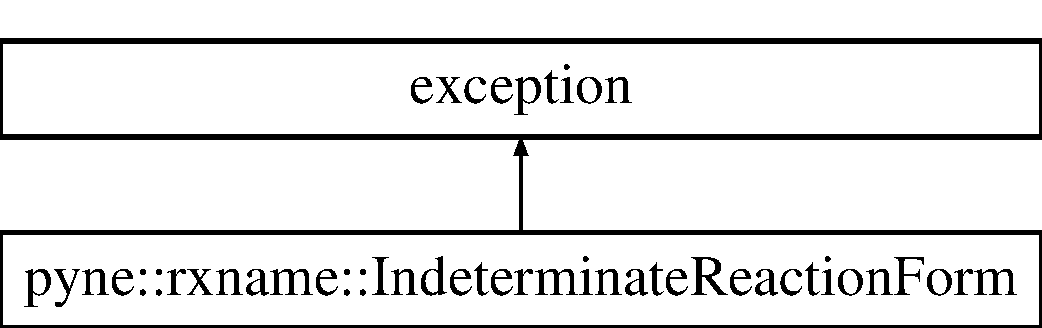
\includegraphics[height=2.000000cm]{classpyne_1_1rxname_1_1_indeterminate_reaction_form}
\end{center}
\end{figure}
\subsection*{Public Member Functions}
\begin{DoxyCompactItemize}
\item 
\hyperlink{classpyne_1_1rxname_1_1_indeterminate_reaction_form_a27a58bf85e1d384d5cf614ef72873e1b}{Indeterminate\+Reaction\+Form} ()\hypertarget{classpyne_1_1rxname_1_1_indeterminate_reaction_form_a27a58bf85e1d384d5cf614ef72873e1b}{}\label{classpyne_1_1rxname_1_1_indeterminate_reaction_form_a27a58bf85e1d384d5cf614ef72873e1b}

\begin{DoxyCompactList}\small\item\em default constructor \end{DoxyCompactList}\item 
\hyperlink{classpyne_1_1rxname_1_1_indeterminate_reaction_form_a7df25775691de519d2ccdc9a25a4e5b2}{$\sim$\+Indeterminate\+Reaction\+Form} ()  throw ()\hypertarget{classpyne_1_1rxname_1_1_indeterminate_reaction_form_a7df25775691de519d2ccdc9a25a4e5b2}{}\label{classpyne_1_1rxname_1_1_indeterminate_reaction_form_a7df25775691de519d2ccdc9a25a4e5b2}

\begin{DoxyCompactList}\small\item\em default destructor \end{DoxyCompactList}\item 
\hyperlink{classpyne_1_1rxname_1_1_indeterminate_reaction_form_ad5a88cc1f318df127516265e9f2bdc87}{Indeterminate\+Reaction\+Form} (std\+::string wasptr, std\+::string nowptr)
\item 
\hyperlink{classpyne_1_1rxname_1_1_indeterminate_reaction_form_abcbbdd0a0a16e11b20eadffc1b7af7a4}{Indeterminate\+Reaction\+Form} (std\+::string wasptr, int nowptr)
\item 
\hyperlink{classpyne_1_1rxname_1_1_indeterminate_reaction_form_ae3b4b1af4980744bfe06bdd66f2ef696}{Indeterminate\+Reaction\+Form} (int wasptr, std\+::string nowptr)
\item 
\hyperlink{classpyne_1_1rxname_1_1_indeterminate_reaction_form_a8efd3b1144d39fc11e67f4411c3b5149}{Indeterminate\+Reaction\+Form} (int wasptr, int nowptr)
\item 
virtual const char $\ast$ \hyperlink{classpyne_1_1rxname_1_1_indeterminate_reaction_form_a7a1cf5af3d08aecd0394e7624c4918ed}{what} () const   throw ()\hypertarget{classpyne_1_1rxname_1_1_indeterminate_reaction_form_a7a1cf5af3d08aecd0394e7624c4918ed}{}\label{classpyne_1_1rxname_1_1_indeterminate_reaction_form_a7a1cf5af3d08aecd0394e7624c4918ed}

\begin{DoxyCompactList}\small\item\em Returns a helpful error message containing prior and current reaction state. \end{DoxyCompactList}\end{DoxyCompactItemize}


\subsection{Detailed Description}
Custom exception for declaring a value not to be of ambiquous reaction form. 

\subsection{Constructor \& Destructor Documentation}
\index{pyne\+::rxname\+::\+Indeterminate\+Reaction\+Form@{pyne\+::rxname\+::\+Indeterminate\+Reaction\+Form}!Indeterminate\+Reaction\+Form@{Indeterminate\+Reaction\+Form}}
\index{Indeterminate\+Reaction\+Form@{Indeterminate\+Reaction\+Form}!pyne\+::rxname\+::\+Indeterminate\+Reaction\+Form@{pyne\+::rxname\+::\+Indeterminate\+Reaction\+Form}}
\subsubsection[{\texorpdfstring{Indeterminate\+Reaction\+Form(std\+::string wasptr, std\+::string nowptr)}{IndeterminateReactionForm(std::string wasptr, std::string nowptr)}}]{\setlength{\rightskip}{0pt plus 5cm}pyne\+::rxname\+::\+Indeterminate\+Reaction\+Form\+::\+Indeterminate\+Reaction\+Form (
\begin{DoxyParamCaption}
\item[{std\+::string}]{wasptr, }
\item[{std\+::string}]{nowptr}
\end{DoxyParamCaption}
)\hspace{0.3cm}{\ttfamily [inline]}}\hypertarget{classpyne_1_1rxname_1_1_indeterminate_reaction_form_ad5a88cc1f318df127516265e9f2bdc87}{}\label{classpyne_1_1rxname_1_1_indeterminate_reaction_form_ad5a88cc1f318df127516265e9f2bdc87}
Constructor using original reaction ({\itshape wasptr}) and the eventual state that Py\+NE calculated ({\itshape nowptr}). \index{pyne\+::rxname\+::\+Indeterminate\+Reaction\+Form@{pyne\+::rxname\+::\+Indeterminate\+Reaction\+Form}!Indeterminate\+Reaction\+Form@{Indeterminate\+Reaction\+Form}}
\index{Indeterminate\+Reaction\+Form@{Indeterminate\+Reaction\+Form}!pyne\+::rxname\+::\+Indeterminate\+Reaction\+Form@{pyne\+::rxname\+::\+Indeterminate\+Reaction\+Form}}
\subsubsection[{\texorpdfstring{Indeterminate\+Reaction\+Form(std\+::string wasptr, int nowptr)}{IndeterminateReactionForm(std::string wasptr, int nowptr)}}]{\setlength{\rightskip}{0pt plus 5cm}pyne\+::rxname\+::\+Indeterminate\+Reaction\+Form\+::\+Indeterminate\+Reaction\+Form (
\begin{DoxyParamCaption}
\item[{std\+::string}]{wasptr, }
\item[{int}]{nowptr}
\end{DoxyParamCaption}
)\hspace{0.3cm}{\ttfamily [inline]}}\hypertarget{classpyne_1_1rxname_1_1_indeterminate_reaction_form_abcbbdd0a0a16e11b20eadffc1b7af7a4}{}\label{classpyne_1_1rxname_1_1_indeterminate_reaction_form_abcbbdd0a0a16e11b20eadffc1b7af7a4}
Constructor using original reaction ({\itshape wasptr}) and the eventual state that Py\+NE calculated ({\itshape nowptr}). \index{pyne\+::rxname\+::\+Indeterminate\+Reaction\+Form@{pyne\+::rxname\+::\+Indeterminate\+Reaction\+Form}!Indeterminate\+Reaction\+Form@{Indeterminate\+Reaction\+Form}}
\index{Indeterminate\+Reaction\+Form@{Indeterminate\+Reaction\+Form}!pyne\+::rxname\+::\+Indeterminate\+Reaction\+Form@{pyne\+::rxname\+::\+Indeterminate\+Reaction\+Form}}
\subsubsection[{\texorpdfstring{Indeterminate\+Reaction\+Form(int wasptr, std\+::string nowptr)}{IndeterminateReactionForm(int wasptr, std::string nowptr)}}]{\setlength{\rightskip}{0pt plus 5cm}pyne\+::rxname\+::\+Indeterminate\+Reaction\+Form\+::\+Indeterminate\+Reaction\+Form (
\begin{DoxyParamCaption}
\item[{int}]{wasptr, }
\item[{std\+::string}]{nowptr}
\end{DoxyParamCaption}
)\hspace{0.3cm}{\ttfamily [inline]}}\hypertarget{classpyne_1_1rxname_1_1_indeterminate_reaction_form_ae3b4b1af4980744bfe06bdd66f2ef696}{}\label{classpyne_1_1rxname_1_1_indeterminate_reaction_form_ae3b4b1af4980744bfe06bdd66f2ef696}
Constructor using original reaction ({\itshape wasptr}) and the eventual state that Py\+NE calculated ({\itshape nowptr}). \index{pyne\+::rxname\+::\+Indeterminate\+Reaction\+Form@{pyne\+::rxname\+::\+Indeterminate\+Reaction\+Form}!Indeterminate\+Reaction\+Form@{Indeterminate\+Reaction\+Form}}
\index{Indeterminate\+Reaction\+Form@{Indeterminate\+Reaction\+Form}!pyne\+::rxname\+::\+Indeterminate\+Reaction\+Form@{pyne\+::rxname\+::\+Indeterminate\+Reaction\+Form}}
\subsubsection[{\texorpdfstring{Indeterminate\+Reaction\+Form(int wasptr, int nowptr)}{IndeterminateReactionForm(int wasptr, int nowptr)}}]{\setlength{\rightskip}{0pt plus 5cm}pyne\+::rxname\+::\+Indeterminate\+Reaction\+Form\+::\+Indeterminate\+Reaction\+Form (
\begin{DoxyParamCaption}
\item[{int}]{wasptr, }
\item[{int}]{nowptr}
\end{DoxyParamCaption}
)\hspace{0.3cm}{\ttfamily [inline]}}\hypertarget{classpyne_1_1rxname_1_1_indeterminate_reaction_form_a8efd3b1144d39fc11e67f4411c3b5149}{}\label{classpyne_1_1rxname_1_1_indeterminate_reaction_form_a8efd3b1144d39fc11e67f4411c3b5149}
Constructor using original reaction ({\itshape wasptr}) and the eventual state that Py\+NE calculated ({\itshape nowptr}). 

The documentation for this class was generated from the following file\+:\begin{DoxyCompactItemize}
\item 
/home/ubuntu/\+Documents/pyne.\+github.\+com/src/rxname.\+h\end{DoxyCompactItemize}

\hypertarget{classpyne_1_1_invalid_simple_x_s}{}\section{pyne\+:\+:Invalid\+Simple\+XS Class Reference}
\label{classpyne_1_1_invalid_simple_x_s}\index{pyne\+::\+Invalid\+Simple\+XS@{pyne\+::\+Invalid\+Simple\+XS}}


Custom exception for declaring a \hyperlink{structsimple__xs}{simple\+\_\+xs} request invalid.  




{\ttfamily \#include $<$data.\+h$>$}

Inheritance diagram for pyne\+:\+:Invalid\+Simple\+XS\+:\begin{figure}[H]
\begin{center}
\leavevmode
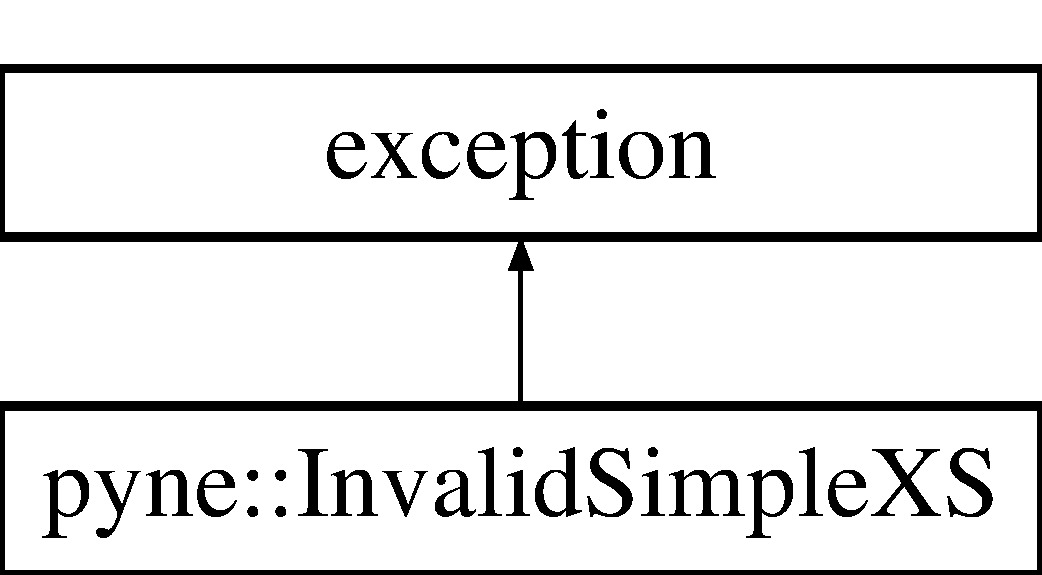
\includegraphics[height=2.000000cm]{classpyne_1_1_invalid_simple_x_s}
\end{center}
\end{figure}
\subsection*{Public Member Functions}
\begin{DoxyCompactItemize}
\item 
\hyperlink{classpyne_1_1_invalid_simple_x_s_ad3bac5f587ea476c11a622024914d074}{Invalid\+Simple\+XS} (std\+::string msg)\hypertarget{classpyne_1_1_invalid_simple_x_s_ad3bac5f587ea476c11a622024914d074}{}\label{classpyne_1_1_invalid_simple_x_s_ad3bac5f587ea476c11a622024914d074}

\begin{DoxyCompactList}\small\item\em Exception thrown if energy group or rxname are invalid. \end{DoxyCompactList}\item 
virtual const char $\ast$ \hyperlink{classpyne_1_1_invalid_simple_x_s_aaafdfd9422833d680a00d7c00263b04a}{what} () const   throw ()\hypertarget{classpyne_1_1_invalid_simple_x_s_aaafdfd9422833d680a00d7c00263b04a}{}\label{classpyne_1_1_invalid_simple_x_s_aaafdfd9422833d680a00d7c00263b04a}

\begin{DoxyCompactList}\small\item\em Exception returns the string passed when thrown. \end{DoxyCompactList}\end{DoxyCompactItemize}


\subsection{Detailed Description}
Custom exception for declaring a \hyperlink{structsimple__xs}{simple\+\_\+xs} request invalid. 

The documentation for this class was generated from the following file\+:\begin{DoxyCompactItemize}
\item 
/home/ubuntu/\+Documents/pyne.\+github.\+com/src/\hyperlink{data_8h}{data.\+h}\end{DoxyCompactItemize}

\hypertarget{structpyne_1_1level__data}{}\section{pyne\+:\+:level\+\_\+data Struct Reference}
\label{structpyne_1_1level__data}\index{pyne\+::level\+\_\+data@{pyne\+::level\+\_\+data}}


a struct matching the \textquotesingle{}/decay/level\+\_\+list\textquotesingle{} table in nuc\+\_\+data.\+h5.  




{\ttfamily \#include $<$data.\+h$>$}

\subsection*{Public Attributes}
\begin{DoxyCompactItemize}
\item 
int \hyperlink{structpyne_1_1level__data_aefac68a7a5aaedafd0b01f459e75adc8}{nuc\+\_\+id}\hypertarget{structpyne_1_1level__data_aefac68a7a5aaedafd0b01f459e75adc8}{}\label{structpyne_1_1level__data_aefac68a7a5aaedafd0b01f459e75adc8}

\begin{DoxyCompactList}\small\item\em state id of nuclide \end{DoxyCompactList}\item 
unsigned int \hyperlink{structpyne_1_1level__data_a52a8e7987f8f2a01fe7142bac5ab6adc}{rx\+\_\+id}\hypertarget{structpyne_1_1level__data_a52a8e7987f8f2a01fe7142bac5ab6adc}{}\label{structpyne_1_1level__data_a52a8e7987f8f2a01fe7142bac5ab6adc}

\begin{DoxyCompactList}\small\item\em rx id of reaction, 0 for basic level data \end{DoxyCompactList}\item 
double \hyperlink{structpyne_1_1level__data_a044daae5c914e096c423b95da1586dc0}{half\+\_\+life}\hypertarget{structpyne_1_1level__data_a044daae5c914e096c423b95da1586dc0}{}\label{structpyne_1_1level__data_a044daae5c914e096c423b95da1586dc0}

\begin{DoxyCompactList}\small\item\em half life \mbox{[}seconds\mbox{]} \end{DoxyCompactList}\item 
double \hyperlink{structpyne_1_1level__data_af029059b5f79cfa2ad22e6f9fcb04ac9}{level}\hypertarget{structpyne_1_1level__data_af029059b5f79cfa2ad22e6f9fcb04ac9}{}\label{structpyne_1_1level__data_af029059b5f79cfa2ad22e6f9fcb04ac9}

\begin{DoxyCompactList}\small\item\em level energy \mbox{[}keV\mbox{]} \end{DoxyCompactList}\item 
double \hyperlink{structpyne_1_1level__data_a5ce97c540e0ce558156e5a43510a4633}{branch\+\_\+ratio}\hypertarget{structpyne_1_1level__data_a5ce97c540e0ce558156e5a43510a4633}{}\label{structpyne_1_1level__data_a5ce97c540e0ce558156e5a43510a4633}

\begin{DoxyCompactList}\small\item\em branch ratio \mbox{[}fraction\mbox{]} \end{DoxyCompactList}\item 
int \hyperlink{structpyne_1_1level__data_a7a71068eed39597f007cc6624727e954}{metastable}\hypertarget{structpyne_1_1level__data_a7a71068eed39597f007cc6624727e954}{}\label{structpyne_1_1level__data_a7a71068eed39597f007cc6624727e954}

\begin{DoxyCompactList}\small\item\em metastable level \mbox{[}int\mbox{]} \end{DoxyCompactList}\item 
char \hyperlink{structpyne_1_1level__data_acabc31aa71741dbc2ea5485ca51da0d6}{special}\hypertarget{structpyne_1_1level__data_acabc31aa71741dbc2ea5485ca51da0d6}{}\label{structpyne_1_1level__data_acabc31aa71741dbc2ea5485ca51da0d6}

\begin{DoxyCompactList}\small\item\em special high-\/spin state \mbox{[}character\mbox{]} \end{DoxyCompactList}\end{DoxyCompactItemize}


\subsection{Detailed Description}
a struct matching the \textquotesingle{}/decay/level\+\_\+list\textquotesingle{} table in nuc\+\_\+data.\+h5. 

The documentation for this struct was generated from the following file\+:\begin{DoxyCompactItemize}
\item 
/home/lucas/opt/gcc-\/6/pyne-\/dev/pyne/src/\hyperlink{data_8h}{data.\+h}\end{DoxyCompactItemize}

\hypertarget{classpyne_1_1_material}{}\section{pyne\+:\+:Material Class Reference}
\label{classpyne_1_1_material}\index{pyne\+::\+Material@{pyne\+::\+Material}}


\hyperlink{classpyne_1_1_material}{Material} composed of nuclides.  




{\ttfamily \#include $<$material.\+h$>$}

\subsection*{Public Member Functions}
\begin{DoxyCompactItemize}
\item 
\hyperlink{classpyne_1_1_material_af9ff0462388696834a886b2e284ccd4e}{Material} ()
\item 
\hyperlink{classpyne_1_1_material_a0704a8fc8a7599cb271c349240f37538}{Material} (\hyperlink{namespacepyne_a86738cecccf4ce3f4ecc2ff6f45ce1a2}{comp\+\_\+map} cm, double m=-\/1.\+0, double d=-\/1.\+0, double apm=-\/1.\+0, Json\+::\+Value attributes=Json\+::\+Value(\hyperlink{namespace_json_a7d654b75c16a57007925868e38212b4eae8386dcfc36d1ae897745f7b4f77a1f6}{Json\+::object\+Value}))
\item 
\hyperlink{classpyne_1_1_material_a9119502ada318009bebedfb429d534d6}{Material} (char $\ast$filename, double m=-\/1.\+0, double d=-\/1.\+0, double apm=-\/1.\+0, Json\+::\+Value attributes=Json\+::\+Value(\hyperlink{namespace_json_a7d654b75c16a57007925868e38212b4eae8386dcfc36d1ae897745f7b4f77a1f6}{Json\+::object\+Value}))
\item 
\hyperlink{classpyne_1_1_material_ad8f2148f252f71de8f699d58003ca050}{Material} (std\+::string filename, double m=-\/1.\+0, double d=-\/1.\+0, double apm=-\/1.\+0, Json\+::\+Value attributes=Json\+::\+Value(\hyperlink{namespace_json_a7d654b75c16a57007925868e38212b4eae8386dcfc36d1ae897745f7b4f77a1f6}{Json\+::object\+Value}))
\item 
\hyperlink{classpyne_1_1_material_ae75f45397f12797356940e62d13fcc6f}{$\sim$\+Material} ()\hypertarget{classpyne_1_1_material_ae75f45397f12797356940e62d13fcc6f}{}\label{classpyne_1_1_material_ae75f45397f12797356940e62d13fcc6f}

\begin{DoxyCompactList}\small\item\em default destructor \end{DoxyCompactList}\item 
void \hyperlink{classpyne_1_1_material_a1d4f70382d3c4ad060977de853d23d6c}{norm\+\_\+comp} ()\hypertarget{classpyne_1_1_material_a1d4f70382d3c4ad060977de853d23d6c}{}\label{classpyne_1_1_material_a1d4f70382d3c4ad060977de853d23d6c}

\begin{DoxyCompactList}\small\item\em Normalizes the mass values in the composition. \end{DoxyCompactList}\item 
void \hyperlink{classpyne_1_1_material_a53c124ac70017813b4893a2f7fe3db6a}{\+\_\+load\+\_\+comp\+\_\+protocol0} (hid\+\_\+t db, std\+::string datapath, int row)
\item 
void \hyperlink{classpyne_1_1_material_a8b46ba10cebb01cd36a5379e363267b1}{\+\_\+load\+\_\+comp\+\_\+protocol1} (hid\+\_\+t db, std\+::string datapath, int row)
\item 
void \hyperlink{classpyne_1_1_material_a8f06385fde86492d1291b35fa982c753}{from\+\_\+hdf5} (char $\ast$filename, char $\ast$datapath, int row=-\/1, int protocol=1)
\item 
void \hyperlink{classpyne_1_1_material_ac6bc51ed739f2f735467baf14716d825}{from\+\_\+hdf5} (std\+::string filename, std\+::string datapath=\char`\"{}/material\char`\"{}, int row=-\/1, int protocol=1)
\item 
void \hyperlink{classpyne_1_1_material_adf226509fcdbf44476019fde3ff2f6ee}{write\+\_\+hdf5} (char $\ast$filename, char $\ast$datapath, char $\ast$nucpath, float row=-\/0.\+0, int chunksize=100)
\item 
void \hyperlink{classpyne_1_1_material_a9c5e1c52faafe841ff2227d08ba7aaf7}{write\+\_\+hdf5} (std\+::string filename, std\+::string datapath=\char`\"{}/material\char`\"{}, std\+::string nucpath=\char`\"{}/nucid\char`\"{}, float row=-\/0.\+0, int chunksize=100)
\item 
std\+::string \hyperlink{classpyne_1_1_material_ac30ed9f082dc76a0c535eb9237a6c528}{mcnp} (std\+::string frac\+\_\+type=\char`\"{}mass\char`\"{})\hypertarget{classpyne_1_1_material_ac30ed9f082dc76a0c535eb9237a6c528}{}\label{classpyne_1_1_material_ac30ed9f082dc76a0c535eb9237a6c528}

\begin{DoxyCompactList}\small\item\em Return an mcnp input deck record as a string. \end{DoxyCompactList}\item 
std\+::string \hyperlink{classpyne_1_1_material_a6bcd10072abbf3e9a8bcaa466f8be569}{fluka} (int id, std\+::string frac\+\_\+type=\char`\"{}mass\char`\"{})
\item 
bool \hyperlink{classpyne_1_1_material_a97461e1c6a87d91ed1293adbe43cb29e}{not\+\_\+fluka\+\_\+builtin} (std\+::string fluka\+\_\+name)
\begin{DoxyCompactList}\small\item\em Convenience function to tell whether a given name needs a material card. \end{DoxyCompactList}\item 
std\+::string \hyperlink{classpyne_1_1_material_af3f7e0865a7a8019e02c2fb3c408c2f3}{fluka\+\_\+material\+\_\+str} (int id)
\begin{DoxyCompactList}\small\item\em High level call to get details and call material\+\_\+component(..) \end{DoxyCompactList}\item 
std\+::string \hyperlink{classpyne_1_1_material_a3b7bc2f7ca3f2c05860004ea27ebcadb}{fluka\+\_\+material\+\_\+component} (int fid, int nucid, std\+::string fluka\+\_\+name)
\begin{DoxyCompactList}\small\item\em Intermediate level call to prepare final info and call material\+\_\+line(..) \end{DoxyCompactList}\item 
std\+::string \hyperlink{classpyne_1_1_material_a269b13dac00eb3ba0ff31feb5bd3b0ca}{fluka\+\_\+material\+\_\+line} (int znum, double \hyperlink{namespacepyne_aaab79c2417fc60c1a248dd702403befb}{atomic\+\_\+mass}, int fid, std\+::string fluka\+\_\+name)
\begin{DoxyCompactList}\small\item\em Format information into a F\+L\+U\+KA material card. \end{DoxyCompactList}\item 
std\+::string \hyperlink{classpyne_1_1_material_ab5fb8d5171b210a7c151d6bb1e180693}{fluka\+\_\+format\+\_\+field} (float field)
\begin{DoxyCompactList}\small\item\em Convenience function to format a single fluka field. \end{DoxyCompactList}\item 
std\+::string \hyperlink{classpyne_1_1_material_a3dd223f881e39c1c6014c2b79c9ee39b}{fluka\+\_\+compound\+\_\+str} (int id, std\+::string frac\+\_\+type=\char`\"{}mass\char`\"{})
\item 
void \hyperlink{classpyne_1_1_material_a28d8f7a7b06110a8be097c8e7b1fc59a}{from\+\_\+text} (char $\ast$filename)\hypertarget{classpyne_1_1_material_a28d8f7a7b06110a8be097c8e7b1fc59a}{}\label{classpyne_1_1_material_a28d8f7a7b06110a8be097c8e7b1fc59a}

\begin{DoxyCompactList}\small\item\em Reads data from a plaintext file at {\itshape filename} into this \hyperlink{classpyne_1_1_material}{Material} instance. \end{DoxyCompactList}\item 
void \hyperlink{classpyne_1_1_material_af74dc1341ac435f41684c935b0c9324f}{from\+\_\+text} (std\+::string filename)\hypertarget{classpyne_1_1_material_af74dc1341ac435f41684c935b0c9324f}{}\label{classpyne_1_1_material_af74dc1341ac435f41684c935b0c9324f}

\begin{DoxyCompactList}\small\item\em Reads data from a plaintext file at {\itshape filename} into this \hyperlink{classpyne_1_1_material}{Material} instance. \end{DoxyCompactList}\item 
void \hyperlink{classpyne_1_1_material_a6d10e7f7dac857f59a89e1664e8b86b6}{write\+\_\+text} (char $\ast$filename)\hypertarget{classpyne_1_1_material_a6d10e7f7dac857f59a89e1664e8b86b6}{}\label{classpyne_1_1_material_a6d10e7f7dac857f59a89e1664e8b86b6}

\begin{DoxyCompactList}\small\item\em Writes the \hyperlink{classpyne_1_1_material}{Material} out to a simple plaintext file readable by \hyperlink{classpyne_1_1_material_a28d8f7a7b06110a8be097c8e7b1fc59a}{from\+\_\+text()}. \end{DoxyCompactList}\item 
void \hyperlink{classpyne_1_1_material_a70706c2bc1f4776ea25932e1a5b2642b}{write\+\_\+text} (std\+::string filename)\hypertarget{classpyne_1_1_material_a70706c2bc1f4776ea25932e1a5b2642b}{}\label{classpyne_1_1_material_a70706c2bc1f4776ea25932e1a5b2642b}

\begin{DoxyCompactList}\small\item\em Writes the \hyperlink{classpyne_1_1_material}{Material} out to a simple plaintext file readable by \hyperlink{classpyne_1_1_material_a28d8f7a7b06110a8be097c8e7b1fc59a}{from\+\_\+text()}. \end{DoxyCompactList}\item 
void \hyperlink{classpyne_1_1_material_a4647c1131cc8940a5e47aa2f42bf8e88}{load\+\_\+json} (Json\+::\+Value)\hypertarget{classpyne_1_1_material_a4647c1131cc8940a5e47aa2f42bf8e88}{}\label{classpyne_1_1_material_a4647c1131cc8940a5e47aa2f42bf8e88}

\begin{DoxyCompactList}\small\item\em Loads a J\+S\+ON instance tree into this \hyperlink{classpyne_1_1_material}{Material}. \end{DoxyCompactList}\item 
Json\+::\+Value \hyperlink{classpyne_1_1_material_af60262ec849d03e9682f9e90542a6e30}{dump\+\_\+json} ()\hypertarget{classpyne_1_1_material_af60262ec849d03e9682f9e90542a6e30}{}\label{classpyne_1_1_material_af60262ec849d03e9682f9e90542a6e30}

\begin{DoxyCompactList}\small\item\em Dumps the \hyperlink{classpyne_1_1_material}{Material} out to a J\+S\+ON instance tree. \end{DoxyCompactList}\item 
void \hyperlink{classpyne_1_1_material_a7a78cc895526f4f4860639c29105a73c}{from\+\_\+json} (char $\ast$filename)\hypertarget{classpyne_1_1_material_a7a78cc895526f4f4860639c29105a73c}{}\label{classpyne_1_1_material_a7a78cc895526f4f4860639c29105a73c}

\begin{DoxyCompactList}\small\item\em Reads data from a J\+S\+ON file at {\itshape filename} into this \hyperlink{classpyne_1_1_material}{Material} instance. \end{DoxyCompactList}\item 
void \hyperlink{classpyne_1_1_material_a8c9791e530b68bd2aace37380aa9a437}{from\+\_\+json} (std\+::string filname)\hypertarget{classpyne_1_1_material_a8c9791e530b68bd2aace37380aa9a437}{}\label{classpyne_1_1_material_a8c9791e530b68bd2aace37380aa9a437}

\begin{DoxyCompactList}\small\item\em Reads data from a J\+S\+ON file at {\itshape filename} into this \hyperlink{classpyne_1_1_material}{Material} instance. \end{DoxyCompactList}\item 
void \hyperlink{classpyne_1_1_material_ab152859c735b74a049e24faa67111a62}{write\+\_\+json} (char $\ast$filename)\hypertarget{classpyne_1_1_material_ab152859c735b74a049e24faa67111a62}{}\label{classpyne_1_1_material_ab152859c735b74a049e24faa67111a62}

\begin{DoxyCompactList}\small\item\em Writes the \hyperlink{classpyne_1_1_material}{Material} out to a J\+S\+ON file. \end{DoxyCompactList}\item 
void \hyperlink{classpyne_1_1_material_a2572b956404b64e2414bfea380324e9a}{write\+\_\+json} (std\+::string filename)\hypertarget{classpyne_1_1_material_a2572b956404b64e2414bfea380324e9a}{}\label{classpyne_1_1_material_a2572b956404b64e2414bfea380324e9a}

\begin{DoxyCompactList}\small\item\em Writes the \hyperlink{classpyne_1_1_material}{Material} out to a J\+S\+ON file. \end{DoxyCompactList}\item 
void \hyperlink{classpyne_1_1_material_ad27e37568bc08020d3886bb6284bc61d}{normalize} ()
\item 
\hyperlink{namespacepyne_a86738cecccf4ce3f4ecc2ff6f45ce1a2}{comp\+\_\+map} \hyperlink{classpyne_1_1_material_ad561ad2e529cbdcc0c73b10b067289fd}{mult\+\_\+by\+\_\+mass} ()
\item 
double \hyperlink{classpyne_1_1_material_a5adf1c262bbabfadf5a8491e7a434ae5}{molecular\+\_\+mass} (double apm=-\/1.\+0)
\item 
\hyperlink{namespacepyne_a86738cecccf4ce3f4ecc2ff6f45ce1a2}{comp\+\_\+map} \hyperlink{classpyne_1_1_material_aae4cbb00f956e2b89fc30ec65124408e}{activity} ()
\item 
\hyperlink{namespacepyne_a86738cecccf4ce3f4ecc2ff6f45ce1a2}{comp\+\_\+map} \hyperlink{classpyne_1_1_material_afa2f1337b64376c13bcece406bbc70f1}{decay\+\_\+heat} ()
\item 
\hyperlink{namespacepyne_a86738cecccf4ce3f4ecc2ff6f45ce1a2}{comp\+\_\+map} \hyperlink{classpyne_1_1_material_a8a55933dccd966f7f3e29d21043bb0d5}{dose\+\_\+per\+\_\+g} (std\+::string dose\+\_\+type, int source=0)
\item 
\hyperlink{classpyne_1_1_material}{Material} \hyperlink{classpyne_1_1_material_a1013d4217c99935396a5f3bc74722bd1}{expand\+\_\+elements} ()
\item 
\hyperlink{classpyne_1_1_material}{Material} {\bfseries collapse\+\_\+elements} (std\+::set$<$ int $>$ exception\+\_\+znum)\hypertarget{classpyne_1_1_material_a87cce5b3c63e3f74c3193db856727a8c}{}\label{classpyne_1_1_material_a87cce5b3c63e3f74c3193db856727a8c}

\item 
\hyperlink{classpyne_1_1_material}{Material} {\bfseries collapse\+\_\+elements} (int $\ast$$\ast$int\+\_\+ptr\+\_\+arry)\hypertarget{classpyne_1_1_material_a58a9f43215bc0c4b826e234b2959a941}{}\label{classpyne_1_1_material_a58a9f43215bc0c4b826e234b2959a941}

\item 
double \hyperlink{classpyne_1_1_material_ac5bbc836d8b9042297444c51506b7439}{mass\+\_\+density} (double num\+\_\+dens=-\/1.\+0, double apm=-\/1.\+0)
\item 
double \hyperlink{classpyne_1_1_material_a25bb43110ee9bd275cbe534c95713acc}{number\+\_\+density} (double mass\+\_\+dens=-\/1.\+0, double apm=-\/1.\+0)
\item 
\hyperlink{classpyne_1_1_material}{Material} \hyperlink{classpyne_1_1_material_a50c2deb6e8513bfb101c5b2992e7f5dc}{sub\+\_\+mat} (std\+::set$<$ int $>$ nucset)
\item 
\hyperlink{classpyne_1_1_material}{Material} \hyperlink{classpyne_1_1_material_a7cd9de1e2a7a80b5beb4946667823b68}{sub\+\_\+mat} (std\+::set$<$ std\+::string $>$ nucset)
\item 
\hyperlink{classpyne_1_1_material}{Material} \hyperlink{classpyne_1_1_material_a17530f493ed5ba0d7f6e9e46c3a49744}{set\+\_\+mat} (std\+::set$<$ int $>$ nucset, double value)
\item 
\hyperlink{classpyne_1_1_material}{Material} \hyperlink{classpyne_1_1_material_a878002d7dfce0dd5a2ed518c6afc6b10}{set\+\_\+mat} (std\+::set$<$ std\+::string $>$ nucset, double value)
\item 
\hyperlink{classpyne_1_1_material}{Material} \hyperlink{classpyne_1_1_material_a34944c4d3c0627ea41d5c7631d080094}{del\+\_\+mat} (std\+::set$<$ int $>$ nucset)
\item 
\hyperlink{classpyne_1_1_material}{Material} \hyperlink{classpyne_1_1_material_a3989e723460e0acffb37163a7f7002c0}{del\+\_\+mat} (std\+::set$<$ std\+::string $>$ nucset)
\item 
\hyperlink{classpyne_1_1_material}{Material} \hyperlink{classpyne_1_1_material_ae7abcf8bf30eb3b2ec862df46e792865}{sub\+\_\+range} (int lower=0, int upper=10000000)\hypertarget{classpyne_1_1_material_ae7abcf8bf30eb3b2ec862df46e792865}{}\label{classpyne_1_1_material_ae7abcf8bf30eb3b2ec862df46e792865}

\begin{DoxyCompactList}\small\item\em Creates a sub-\/\+Material based on a range of id-\/form integers. \end{DoxyCompactList}\item 
\hyperlink{classpyne_1_1_material}{Material} \hyperlink{classpyne_1_1_material_af81eb0e8c7f65792bc699c4aec82bb7e}{set\+\_\+range} (int lower=0, int upper=10000000, double value=0.\+0)
\item 
\hyperlink{classpyne_1_1_material}{Material} \hyperlink{classpyne_1_1_material_a2e5387cd2fb1dea7bf6fdd567529ae6f}{del\+\_\+range} (int lower=0, int upper=10000000)\hypertarget{classpyne_1_1_material_a2e5387cd2fb1dea7bf6fdd567529ae6f}{}\label{classpyne_1_1_material_a2e5387cd2fb1dea7bf6fdd567529ae6f}

\begin{DoxyCompactList}\small\item\em Creates a new \hyperlink{classpyne_1_1_material}{Material} with the all nuclides in the id range removed. \end{DoxyCompactList}\item 
\hyperlink{classpyne_1_1_material}{Material} \hyperlink{classpyne_1_1_material_aa38cb12439e08391849d41f803f03495}{sub\+\_\+elem} (int element)
\item 
\hyperlink{classpyne_1_1_material}{Material} \hyperlink{classpyne_1_1_material_ad5f4191cb47a820be447e0a4b70da96c}{sub\+\_\+lan} ()\hypertarget{classpyne_1_1_material_ad5f4191cb47a820be447e0a4b70da96c}{}\label{classpyne_1_1_material_ad5f4191cb47a820be447e0a4b70da96c}

\begin{DoxyCompactList}\small\item\em Creates a sub-\/\+Material of only lanthanides. \end{DoxyCompactList}\item 
\hyperlink{classpyne_1_1_material}{Material} \hyperlink{classpyne_1_1_material_addb8d9eb230f9782ebf2f5381c35ccde}{sub\+\_\+act} ()\hypertarget{classpyne_1_1_material_addb8d9eb230f9782ebf2f5381c35ccde}{}\label{classpyne_1_1_material_addb8d9eb230f9782ebf2f5381c35ccde}

\begin{DoxyCompactList}\small\item\em Creates a sub-\/\+Material of only actinides. \end{DoxyCompactList}\item 
\hyperlink{classpyne_1_1_material}{Material} \hyperlink{classpyne_1_1_material_ab0d02f754f1570cca42b33258d1db997}{sub\+\_\+tru} ()\hypertarget{classpyne_1_1_material_ab0d02f754f1570cca42b33258d1db997}{}\label{classpyne_1_1_material_ab0d02f754f1570cca42b33258d1db997}

\begin{DoxyCompactList}\small\item\em Creates a sub-\/\+Material of only transuranics. \end{DoxyCompactList}\item 
\hyperlink{classpyne_1_1_material}{Material} \hyperlink{classpyne_1_1_material_a9d0e3214dda2be1f96a61cf8e379c086}{sub\+\_\+ma} ()\hypertarget{classpyne_1_1_material_a9d0e3214dda2be1f96a61cf8e379c086}{}\label{classpyne_1_1_material_a9d0e3214dda2be1f96a61cf8e379c086}

\begin{DoxyCompactList}\small\item\em Creates a sub-\/\+Material of only minor actinides. \end{DoxyCompactList}\item 
\hyperlink{classpyne_1_1_material}{Material} \hyperlink{classpyne_1_1_material_a514e831b1a9fa7eefad69a89ca81e36d}{sub\+\_\+fp} ()\hypertarget{classpyne_1_1_material_a514e831b1a9fa7eefad69a89ca81e36d}{}\label{classpyne_1_1_material_a514e831b1a9fa7eefad69a89ca81e36d}

\begin{DoxyCompactList}\small\item\em Creates a sub-\/\+Material of only fission products. \end{DoxyCompactList}\item 
std\+::map$<$ int, double $>$ \hyperlink{classpyne_1_1_material_a89a5ef5a4bfca961981a46a4252299fd}{to\+\_\+atom\+\_\+frac} ()
\item 
void \hyperlink{classpyne_1_1_material_a2db9572599c20eb0d17bd0993766f792}{from\+\_\+atom\+\_\+frac} (std\+::map$<$ int, double $>$ atom\+\_\+fracs)
\item 
std\+::map$<$ int, double $>$ \hyperlink{classpyne_1_1_material_adfc05d7c09a0908047a9b733aa7c78b1}{to\+\_\+atom\+\_\+dens} ()
\item 
std\+::vector$<$ std\+::pair$<$ double, double $>$ $>$ \hyperlink{classpyne_1_1_material_a2e2721b8ec8fde2d2e08379b39220d00}{gammas} ()
\item 
std\+::vector$<$ std\+::pair$<$ double, double $>$ $>$ \hyperlink{classpyne_1_1_material_a24fbf883f1623dccc4053106041510d5}{xrays} ()
\item 
std\+::vector$<$ std\+::pair$<$ double, double $>$ $>$ \hyperlink{classpyne_1_1_material_a3630f6f54a7ff6355da0b76b4d0e35a1}{photons} (bool norm)
\item 
std\+::vector$<$ std\+::pair$<$ double, double $>$ $>$ \hyperlink{classpyne_1_1_material_a114deb10e8d118bbd37ade0fbce5253d}{normalize\+\_\+radioactivity} (std\+::vector$<$ std\+::pair$<$ double, double $>$ $>$ unnormed)
\item 
\hyperlink{classpyne_1_1_material}{Material} \hyperlink{classpyne_1_1_material_a1b9decf23001574896c3413265677307}{decay} (double t)\hypertarget{classpyne_1_1_material_a1b9decf23001574896c3413265677307}{}\label{classpyne_1_1_material_a1b9decf23001574896c3413265677307}

\begin{DoxyCompactList}\small\item\em Decays this material for a given amount of time in seconds. \end{DoxyCompactList}\item 
\hyperlink{classpyne_1_1_material}{Material} \hyperlink{classpyne_1_1_material_a97bae8b18322f26e1cd87d8909ce42b6}{operator+} (double)\hypertarget{classpyne_1_1_material_a97bae8b18322f26e1cd87d8909ce42b6}{}\label{classpyne_1_1_material_a97bae8b18322f26e1cd87d8909ce42b6}

\begin{DoxyCompactList}\small\item\em Adds mass to a material instance. \end{DoxyCompactList}\item 
\hyperlink{classpyne_1_1_material}{Material} \hyperlink{classpyne_1_1_material_a1913e1a1b525352bf4f0b4155b6d39b7}{operator+} (\hyperlink{classpyne_1_1_material}{Material})\hypertarget{classpyne_1_1_material_a1913e1a1b525352bf4f0b4155b6d39b7}{}\label{classpyne_1_1_material_a1913e1a1b525352bf4f0b4155b6d39b7}

\begin{DoxyCompactList}\small\item\em Adds two materials together. \end{DoxyCompactList}\item 
\hyperlink{classpyne_1_1_material}{Material} \hyperlink{classpyne_1_1_material_a6a924c97822bc791e0b47d4940c8bea3}{operator$\ast$} (double)\hypertarget{classpyne_1_1_material_a6a924c97822bc791e0b47d4940c8bea3}{}\label{classpyne_1_1_material_a6a924c97822bc791e0b47d4940c8bea3}

\begin{DoxyCompactList}\small\item\em Multiplies a material\textquotesingle{}s mass. \end{DoxyCompactList}\item 
\hyperlink{classpyne_1_1_material}{Material} \hyperlink{classpyne_1_1_material_ac9b6ba67915ed4adb763b1c68ef5eb98}{operator/} (double)\hypertarget{classpyne_1_1_material_ac9b6ba67915ed4adb763b1c68ef5eb98}{}\label{classpyne_1_1_material_ac9b6ba67915ed4adb763b1c68ef5eb98}

\begin{DoxyCompactList}\small\item\em Divides a material\textquotesingle{}s mass. \end{DoxyCompactList}\end{DoxyCompactItemize}
\subsection*{Public Attributes}
\begin{DoxyCompactItemize}
\item 
\hyperlink{namespacepyne_a86738cecccf4ce3f4ecc2ff6f45ce1a2}{comp\+\_\+map} \hyperlink{classpyne_1_1_material_a2b0e850a66f2b8cb2b106307a00a18ed}{comp}\hypertarget{classpyne_1_1_material_a2b0e850a66f2b8cb2b106307a00a18ed}{}\label{classpyne_1_1_material_a2b0e850a66f2b8cb2b106307a00a18ed}

\begin{DoxyCompactList}\small\item\em composition, maps nuclides in id form to normalized mass weights. \end{DoxyCompactList}\item 
double \hyperlink{classpyne_1_1_material_a729ebba0be2879f26f1fcf3b100d3b5d}{mass}\hypertarget{classpyne_1_1_material_a729ebba0be2879f26f1fcf3b100d3b5d}{}\label{classpyne_1_1_material_a729ebba0be2879f26f1fcf3b100d3b5d}

\begin{DoxyCompactList}\small\item\em mass (in arbitrary units) of the \hyperlink{classpyne_1_1_material}{Material}. \end{DoxyCompactList}\item 
double \hyperlink{classpyne_1_1_material_a916eb7ed0143844a505c454d47755ab0}{density}\hypertarget{classpyne_1_1_material_a916eb7ed0143844a505c454d47755ab0}{}\label{classpyne_1_1_material_a916eb7ed0143844a505c454d47755ab0}

\begin{DoxyCompactList}\small\item\em density (in arbitrary units) of the \hyperlink{classpyne_1_1_material}{Material}. \end{DoxyCompactList}\item 
double \hyperlink{classpyne_1_1_material_a7ddff1aaebc94bcda22d3422c093a756}{atoms\+\_\+per\+\_\+molecule}
\item 
Json\+::\+Value \hyperlink{classpyne_1_1_material_aee299ae39a32a7ff98e14c2aa3eabe32}{metadata}\hypertarget{classpyne_1_1_material_aee299ae39a32a7ff98e14c2aa3eabe32}{}\label{classpyne_1_1_material_aee299ae39a32a7ff98e14c2aa3eabe32}

\begin{DoxyCompactList}\small\item\em container for arbitrary metadata, following the J\+S\+ON rules. \end{DoxyCompactList}\end{DoxyCompactItemize}
\subsection*{Protected Member Functions}
\begin{DoxyCompactItemize}
\item 
double \hyperlink{classpyne_1_1_material_a6bfe2556962da33cc05eb1e88bdebf42}{get\+\_\+comp\+\_\+sum} ()\hypertarget{classpyne_1_1_material_a6bfe2556962da33cc05eb1e88bdebf42}{}\label{classpyne_1_1_material_a6bfe2556962da33cc05eb1e88bdebf42}

\begin{DoxyCompactList}\small\item\em Computes the total mass stored in the composition. \end{DoxyCompactList}\end{DoxyCompactItemize}


\subsection{Detailed Description}
\hyperlink{classpyne_1_1_material}{Material} composed of nuclides. 

\subsection{Constructor \& Destructor Documentation}
\index{pyne\+::\+Material@{pyne\+::\+Material}!Material@{Material}}
\index{Material@{Material}!pyne\+::\+Material@{pyne\+::\+Material}}
\subsubsection[{\texorpdfstring{Material()}{Material()}}]{\setlength{\rightskip}{0pt plus 5cm}pyne\+::\+Material\+::\+Material (
\begin{DoxyParamCaption}
{}
\end{DoxyParamCaption}
)}\hypertarget{classpyne_1_1_material_af9ff0462388696834a886b2e284ccd4e}{}\label{classpyne_1_1_material_af9ff0462388696834a886b2e284ccd4e}
empty constructor \index{pyne\+::\+Material@{pyne\+::\+Material}!Material@{Material}}
\index{Material@{Material}!pyne\+::\+Material@{pyne\+::\+Material}}
\subsubsection[{\texorpdfstring{Material(comp\+\_\+map cm, double m=-\/1.\+0, double d=-\/1.\+0, double apm=-\/1.\+0, Json\+::\+Value attributes=\+Json\+::\+Value(\+Json\+::object\+Value))}{Material(comp_map cm, double m=-1.0, double d=-1.0, double apm=-1.0, Json::Value attributes=Json::Value(Json::objectValue))}}]{\setlength{\rightskip}{0pt plus 5cm}pyne\+::\+Material\+::\+Material (
\begin{DoxyParamCaption}
\item[{{\bf pyne\+::comp\+\_\+map}}]{cm, }
\item[{double}]{m = {\ttfamily -\/1.0}, }
\item[{double}]{d = {\ttfamily -\/1.0}, }
\item[{double}]{apm = {\ttfamily -\/1.0}, }
\item[{Json\+::\+Value}]{attributes = {\ttfamily Json\+:\+:Value({\bf Json\+::object\+Value})}}
\end{DoxyParamCaption}
)}\hypertarget{classpyne_1_1_material_a0704a8fc8a7599cb271c349240f37538}{}\label{classpyne_1_1_material_a0704a8fc8a7599cb271c349240f37538}
Constructor from composition map 
\begin{DoxyParams}{Parameters}
{\em cm} & composition map \\
\hline
{\em m} & mass value, the mass is set to the sum of the values in the composition if {\itshape m} is negative. \\
\hline
{\em d} & density value \\
\hline
{\em apm} & atoms per mole \\
\hline
{\em attributes} & initial metadata \\
\hline
\end{DoxyParams}
\index{pyne\+::\+Material@{pyne\+::\+Material}!Material@{Material}}
\index{Material@{Material}!pyne\+::\+Material@{pyne\+::\+Material}}
\subsubsection[{\texorpdfstring{Material(char $\ast$filename, double m=-\/1.\+0, double d=-\/1.\+0, double apm=-\/1.\+0, Json\+::\+Value attributes=\+Json\+::\+Value(\+Json\+::object\+Value))}{Material(char *filename, double m=-1.0, double d=-1.0, double apm=-1.0, Json::Value attributes=Json::Value(Json::objectValue))}}]{\setlength{\rightskip}{0pt plus 5cm}pyne\+::\+Material\+::\+Material (
\begin{DoxyParamCaption}
\item[{char $\ast$}]{filename, }
\item[{double}]{m = {\ttfamily -\/1.0}, }
\item[{double}]{d = {\ttfamily -\/1.0}, }
\item[{double}]{apm = {\ttfamily -\/1.0}, }
\item[{Json\+::\+Value}]{attributes = {\ttfamily Json\+:\+:Value({\bf Json\+::object\+Value})}}
\end{DoxyParamCaption}
)}\hypertarget{classpyne_1_1_material_a9119502ada318009bebedfb429d534d6}{}\label{classpyne_1_1_material_a9119502ada318009bebedfb429d534d6}
Constructor from file 
\begin{DoxyParams}{Parameters}
{\em filename} & path to file on disk, this file may be either in plaintext or H\+D\+F5 format. \\
\hline
{\em m} & mass value, the mass is set to the sum of the values in the composition if {\itshape m} is negative, may be overridden by the value from disk. \\
\hline
{\em d} & density value, may be overridden by the value from disk. \\
\hline
{\em apm} & atoms per mole, may be overridden by the value from disk. \\
\hline
{\em attributes} & initial metadata, may be overridden by the value from disk. \\
\hline
\end{DoxyParams}
\index{pyne\+::\+Material@{pyne\+::\+Material}!Material@{Material}}
\index{Material@{Material}!pyne\+::\+Material@{pyne\+::\+Material}}
\subsubsection[{\texorpdfstring{Material(std\+::string filename, double m=-\/1.\+0, double d=-\/1.\+0, double apm=-\/1.\+0, Json\+::\+Value attributes=\+Json\+::\+Value(\+Json\+::object\+Value))}{Material(std::string filename, double m=-1.0, double d=-1.0, double apm=-1.0, Json::Value attributes=Json::Value(Json::objectValue))}}]{\setlength{\rightskip}{0pt plus 5cm}pyne\+::\+Material\+::\+Material (
\begin{DoxyParamCaption}
\item[{std\+::string}]{filename, }
\item[{double}]{m = {\ttfamily -\/1.0}, }
\item[{double}]{d = {\ttfamily -\/1.0}, }
\item[{double}]{apm = {\ttfamily -\/1.0}, }
\item[{Json\+::\+Value}]{attributes = {\ttfamily Json\+:\+:Value({\bf Json\+::object\+Value})}}
\end{DoxyParamCaption}
)}\hypertarget{classpyne_1_1_material_ad8f2148f252f71de8f699d58003ca050}{}\label{classpyne_1_1_material_ad8f2148f252f71de8f699d58003ca050}
Constructor from file 
\begin{DoxyParams}{Parameters}
{\em filename} & path to file on disk, this file may be either in plaintext or H\+D\+F5 format. \\
\hline
{\em m} & mass value, the mass is set to the sum of the values in the composition if {\itshape m} is negative, may be overridden by the value from disk. \\
\hline
{\em d} & density value, may be overridden by the value from disk. \\
\hline
{\em apm} & atoms per mole, may be overridden by the value from disk. \\
\hline
{\em attributes} & initial metadata, may be overridden by the value from disk. \\
\hline
\end{DoxyParams}


\subsection{Member Function Documentation}
\index{pyne\+::\+Material@{pyne\+::\+Material}!\+\_\+load\+\_\+comp\+\_\+protocol0@{\+\_\+load\+\_\+comp\+\_\+protocol0}}
\index{\+\_\+load\+\_\+comp\+\_\+protocol0@{\+\_\+load\+\_\+comp\+\_\+protocol0}!pyne\+::\+Material@{pyne\+::\+Material}}
\subsubsection[{\texorpdfstring{\+\_\+load\+\_\+comp\+\_\+protocol0(hid\+\_\+t db, std\+::string datapath, int row)}{_load_comp_protocol0(hid_t db, std::string datapath, int row)}}]{\setlength{\rightskip}{0pt plus 5cm}void pyne\+::\+Material\+::\+\_\+load\+\_\+comp\+\_\+protocol0 (
\begin{DoxyParamCaption}
\item[{hid\+\_\+t}]{db, }
\item[{std\+::string}]{datapath, }
\item[{int}]{row}
\end{DoxyParamCaption}
)}\hypertarget{classpyne_1_1_material_a53c124ac70017813b4893a2f7fe3db6a}{}\label{classpyne_1_1_material_a53c124ac70017813b4893a2f7fe3db6a}
Loads the matrial composition from an H\+D\+F5 file according to the layout defined by protocol 0. This protocol is depratacted. 
\begin{DoxyParams}{Parameters}
{\em db} & H\+D\+F5 id for the open H\+D\+F5 file. \\
\hline
{\em datapath} & Path to the base node for the material in {\itshape db}. \\
\hline
{\em row} & The index to read out, may be negative. \\
\hline
\end{DoxyParams}
\index{pyne\+::\+Material@{pyne\+::\+Material}!\+\_\+load\+\_\+comp\+\_\+protocol1@{\+\_\+load\+\_\+comp\+\_\+protocol1}}
\index{\+\_\+load\+\_\+comp\+\_\+protocol1@{\+\_\+load\+\_\+comp\+\_\+protocol1}!pyne\+::\+Material@{pyne\+::\+Material}}
\subsubsection[{\texorpdfstring{\+\_\+load\+\_\+comp\+\_\+protocol1(hid\+\_\+t db, std\+::string datapath, int row)}{_load_comp_protocol1(hid_t db, std::string datapath, int row)}}]{\setlength{\rightskip}{0pt plus 5cm}void pyne\+::\+Material\+::\+\_\+load\+\_\+comp\+\_\+protocol1 (
\begin{DoxyParamCaption}
\item[{hid\+\_\+t}]{db, }
\item[{std\+::string}]{datapath, }
\item[{int}]{row}
\end{DoxyParamCaption}
)}\hypertarget{classpyne_1_1_material_a8b46ba10cebb01cd36a5379e363267b1}{}\label{classpyne_1_1_material_a8b46ba10cebb01cd36a5379e363267b1}
Loads the matrial composition from an H\+D\+F5 file according to the layout defined by protocol 1. This protocol should be used in favor of protocol 0. 
\begin{DoxyParams}{Parameters}
{\em db} & H\+D\+F5 id for the open H\+D\+F5 file. \\
\hline
{\em datapath} & Path to the base node for the material in {\itshape db}. \\
\hline
{\em row} & The index to read out, may be negative. \\
\hline
\end{DoxyParams}
\index{pyne\+::\+Material@{pyne\+::\+Material}!activity@{activity}}
\index{activity@{activity}!pyne\+::\+Material@{pyne\+::\+Material}}
\subsubsection[{\texorpdfstring{activity()}{activity()}}]{\setlength{\rightskip}{0pt plus 5cm}{\bf pyne\+::comp\+\_\+map} pyne\+::\+Material\+::activity (
\begin{DoxyParamCaption}
{}
\end{DoxyParamCaption}
)}\hypertarget{classpyne_1_1_material_aae4cbb00f956e2b89fc30ec65124408e}{}\label{classpyne_1_1_material_aae4cbb00f956e2b89fc30ec65124408e}
Calculates the activity of a material based on the composition and each nuclide\textquotesingle{}s mass, decay\+\_\+const, and atmoic\+\_\+mass. \index{pyne\+::\+Material@{pyne\+::\+Material}!decay\+\_\+heat@{decay\+\_\+heat}}
\index{decay\+\_\+heat@{decay\+\_\+heat}!pyne\+::\+Material@{pyne\+::\+Material}}
\subsubsection[{\texorpdfstring{decay\+\_\+heat()}{decay_heat()}}]{\setlength{\rightskip}{0pt plus 5cm}{\bf pyne\+::comp\+\_\+map} pyne\+::\+Material\+::decay\+\_\+heat (
\begin{DoxyParamCaption}
{}
\end{DoxyParamCaption}
)}\hypertarget{classpyne_1_1_material_afa2f1337b64376c13bcece406bbc70f1}{}\label{classpyne_1_1_material_afa2f1337b64376c13bcece406bbc70f1}
Calculates the decay heat of a material based on the composition and each nuclide\textquotesingle{}s mass, q\+\_\+val, decay\+\_\+const, and atomic\+\_\+mass. This assumes input mass of grams. Return values is in megawatts. \index{pyne\+::\+Material@{pyne\+::\+Material}!del\+\_\+mat@{del\+\_\+mat}}
\index{del\+\_\+mat@{del\+\_\+mat}!pyne\+::\+Material@{pyne\+::\+Material}}
\subsubsection[{\texorpdfstring{del\+\_\+mat(std\+::set$<$ int $>$ nucset)}{del_mat(std::set< int > nucset)}}]{\setlength{\rightskip}{0pt plus 5cm}{\bf pyne\+::\+Material} pyne\+::\+Material\+::del\+\_\+mat (
\begin{DoxyParamCaption}
\item[{std\+::set$<$ int $>$}]{nucset}
\end{DoxyParamCaption}
)}\hypertarget{classpyne_1_1_material_a34944c4d3c0627ea41d5c7631d080094}{}\label{classpyne_1_1_material_a34944c4d3c0627ea41d5c7631d080094}
Creates a new \hyperlink{classpyne_1_1_material}{Material} with the all nuclides in {\itshape nucset} removed. Elements of {\itshape nucset} may be either in id form or simple Z numbers. \index{pyne\+::\+Material@{pyne\+::\+Material}!del\+\_\+mat@{del\+\_\+mat}}
\index{del\+\_\+mat@{del\+\_\+mat}!pyne\+::\+Material@{pyne\+::\+Material}}
\subsubsection[{\texorpdfstring{del\+\_\+mat(std\+::set$<$ std\+::string $>$ nucset)}{del_mat(std::set< std::string > nucset)}}]{\setlength{\rightskip}{0pt plus 5cm}{\bf pyne\+::\+Material} pyne\+::\+Material\+::del\+\_\+mat (
\begin{DoxyParamCaption}
\item[{std\+::set$<$ std\+::string $>$}]{nucset}
\end{DoxyParamCaption}
)}\hypertarget{classpyne_1_1_material_a3989e723460e0acffb37163a7f7002c0}{}\label{classpyne_1_1_material_a3989e723460e0acffb37163a7f7002c0}
Creates a new \hyperlink{classpyne_1_1_material}{Material} with the all nuclides in {\itshape nucset} removed. Elements of {\itshape nucset} may be in any form. \index{pyne\+::\+Material@{pyne\+::\+Material}!dose\+\_\+per\+\_\+g@{dose\+\_\+per\+\_\+g}}
\index{dose\+\_\+per\+\_\+g@{dose\+\_\+per\+\_\+g}!pyne\+::\+Material@{pyne\+::\+Material}}
\subsubsection[{\texorpdfstring{dose\+\_\+per\+\_\+g(std\+::string dose\+\_\+type, int source=0)}{dose_per_g(std::string dose_type, int source=0)}}]{\setlength{\rightskip}{0pt plus 5cm}{\bf pyne\+::comp\+\_\+map} pyne\+::\+Material\+::dose\+\_\+per\+\_\+g (
\begin{DoxyParamCaption}
\item[{std\+::string}]{dose\+\_\+type, }
\item[{int}]{source = {\ttfamily 0}}
\end{DoxyParamCaption}
)}\hypertarget{classpyne_1_1_material_a8a55933dccd966f7f3e29d21043bb0d5}{}\label{classpyne_1_1_material_a8a55933dccd966f7f3e29d21043bb0d5}
Caclulates the dose per gram using the composition of the the material, the dose type desired, and the source for dose factors dose\+\_\+type is one of\+: ext\+\_\+air -- returns mrem/h per g per m$^\wedge$3 ext\+\_\+soil -- returns mrem/h per g per m$^\wedge$2 ingest -- returns mrem per g inhale -- returns mrem per g source is\+: \{E\+PA=0, D\+OE=1, G\+E\+N\+II=2\}, default is E\+PA \index{pyne\+::\+Material@{pyne\+::\+Material}!expand\+\_\+elements@{expand\+\_\+elements}}
\index{expand\+\_\+elements@{expand\+\_\+elements}!pyne\+::\+Material@{pyne\+::\+Material}}
\subsubsection[{\texorpdfstring{expand\+\_\+elements()}{expand_elements()}}]{\setlength{\rightskip}{0pt plus 5cm}{\bf pyne\+::\+Material} pyne\+::\+Material\+::expand\+\_\+elements (
\begin{DoxyParamCaption}
{}
\end{DoxyParamCaption}
)}\hypertarget{classpyne_1_1_material_a1013d4217c99935396a5f3bc74722bd1}{}\label{classpyne_1_1_material_a1013d4217c99935396a5f3bc74722bd1}
Returns a copy of the current material where all natural elements in the composition are expanded to their natural isotopic abundances. \index{pyne\+::\+Material@{pyne\+::\+Material}!fluka@{fluka}}
\index{fluka@{fluka}!pyne\+::\+Material@{pyne\+::\+Material}}
\subsubsection[{\texorpdfstring{fluka(int id, std\+::string frac\+\_\+type=""mass"")}{fluka(int id, std::string frac_type="mass")}}]{\setlength{\rightskip}{0pt plus 5cm}std\+::string pyne\+::\+Material\+::fluka (
\begin{DoxyParamCaption}
\item[{int}]{id, }
\item[{std\+::string}]{frac\+\_\+type = {\ttfamily \char`\"{}mass\char`\"{}}}
\end{DoxyParamCaption}
)}\hypertarget{classpyne_1_1_material_a6bcd10072abbf3e9a8bcaa466f8be569}{}\label{classpyne_1_1_material_a6bcd10072abbf3e9a8bcaa466f8be569}
Return a fluka input deck M\+A\+T\+E\+R\+I\+AL card as a string

-\/-\/-\/-\/-\/-\/-\/-\/-\/-\/-\/-\/-\/-\/-\/-\/-\/-\/-\/-\/-\/-\/-\/-\/-\/-\/-\/-\/-\/-\/-\/-\/-\/-\/-\/-\/-\/-\/-\/-\/-\/-\/-\/-\/-\/-\/-\/-\/-\/-\/-\/-\/-\/-\/-\/-\/-\/-\/-\/-\/-\/-\/-\/-\/-\/-\/-\/-\/-\/-\/-\/-\/---// fluka -\/-\/-\/-\/-\/-\/-\/-\/-\/-\/-\/-\/-\/-\/-\/-\/-\/-\/-\/-\/-\/-\/-\/-\/-\/-\/-\/-\/-\/-\/-\/-\/-\/-\/-\/-\/-\/-\/-\/-\/-\/-\/-\/-\/-\/-\/-\/-\/-\/-\/-\/-\/-\/-\/-\/-\/-\/-\/-\/-\/-\/-\/-\/-\/-\/-\/-\/-\/-\/-\/-\/-\/---// Main external call \index{pyne\+::\+Material@{pyne\+::\+Material}!fluka\+\_\+compound\+\_\+str@{fluka\+\_\+compound\+\_\+str}}
\index{fluka\+\_\+compound\+\_\+str@{fluka\+\_\+compound\+\_\+str}!pyne\+::\+Material@{pyne\+::\+Material}}
\subsubsection[{\texorpdfstring{fluka\+\_\+compound\+\_\+str(int id, std\+::string frac\+\_\+type=""mass"")}{fluka_compound_str(int id, std::string frac_type="mass")}}]{\setlength{\rightskip}{0pt plus 5cm}std\+::string pyne\+::\+Material\+::fluka\+\_\+compound\+\_\+str (
\begin{DoxyParamCaption}
\item[{int}]{id, }
\item[{std\+::string}]{frac\+\_\+type = {\ttfamily \char`\"{}mass\char`\"{}}}
\end{DoxyParamCaption}
)}\hypertarget{classpyne_1_1_material_a3dd223f881e39c1c6014c2b79c9ee39b}{}\label{classpyne_1_1_material_a3dd223f881e39c1c6014c2b79c9ee39b}
Return F\+L\+U\+KA compound card and the material card for the named compound but not the material cards of the components

-\/-\/-\/-\/-\/-\/-\/-\/-\/-\/-\/-\/-\/-\/-\/-\/-\/-\/-\/-\/-\/-\/-\/-\/-\/-\/-\/-\/-\/-\/-\/-\/-\/-\/-\/-\/-\/-\/-\/-\/-\/-\/-\/-\/-\/-\/-\/-\/-\/-\/-\/-\/-\/-\/-\/-\/-\/-\/-\/-\/-\/-\/-\/-\/-\/-\/-\/-\/-\/-\/-\/-\/---// fluka\+\_\+compound\+\_\+str -\/-\/-\/-\/-\/-\/-\/-\/-\/-\/-\/-\/-\/-\/-\/-\/-\/-\/-\/-\/-\/-\/-\/-\/-\/-\/-\/-\/-\/-\/-\/-\/-\/-\/-\/-\/-\/-\/-\/-\/-\/-\/-\/-\/-\/-\/-\/-\/-\/-\/-\/-\/-\/-\/-\/-\/-\/-\/-\/-\/-\/-\/-\/-\/-\/-\/-\/-\/-\/-\/-\/-\/---// Returns -- M\+A\+T\+E\+R\+I\+AL line for compound -- C\+O\+M\+P\+O\+U\+ND lines \index{pyne\+::\+Material@{pyne\+::\+Material}!fluka\+\_\+format\+\_\+field@{fluka\+\_\+format\+\_\+field}}
\index{fluka\+\_\+format\+\_\+field@{fluka\+\_\+format\+\_\+field}!pyne\+::\+Material@{pyne\+::\+Material}}
\subsubsection[{\texorpdfstring{fluka\+\_\+format\+\_\+field(float field)}{fluka_format_field(float field)}}]{\setlength{\rightskip}{0pt plus 5cm}std\+::string pyne\+::\+Material\+::fluka\+\_\+format\+\_\+field (
\begin{DoxyParamCaption}
\item[{float}]{field}
\end{DoxyParamCaption}
)}\hypertarget{classpyne_1_1_material_ab5fb8d5171b210a7c151d6bb1e180693}{}\label{classpyne_1_1_material_ab5fb8d5171b210a7c151d6bb1e180693}


Convenience function to format a single fluka field. 

-\/-\/-\/-\/-\/-\/-\/-\/-\/-\/-\/-\/-\/-\/-\/-\/-\/-\/-\/-\/-\/-\/-\/-\/-\/-\/-\/-\/-\/-\/-\/-\/-\/-\/-\/-\/-\/-\/-\/-\/-\/-\/-\/-\/-\/-\/-\/-\/-\/-\/-\/-\/-\/-\/-\/-\/-\/-\/-\/-\/-\/-\/-\/-\/-\/-\/-\/-\/-\/-\/-\/-\/---// fluka\+\_\+format\+\_\+field -\/-\/-\/-\/-\/-\/-\/-\/-\/-\/-\/-\/-\/-\/-\/-\/-\/-\/-\/-\/-\/-\/-\/-\/-\/-\/-\/-\/-\/-\/-\/-\/-\/-\/-\/-\/-\/-\/-\/-\/-\/-\/-\/-\/-\/-\/-\/-\/-\/-\/-\/-\/-\/-\/-\/-\/-\/-\/-\/-\/-\/-\/-\/-\/-\/-\/-\/-\/-\/-\/-\/-\/---// Convenience function that returns a 10-\/character formatted string 999 -\/$>$ 999. 999.\+12 -\/$>$ 999.\+12 999.\+123 -\/$>$ 999.\+123 999.\+1234 -\/$>$ 999.\+123 \index{pyne\+::\+Material@{pyne\+::\+Material}!fluka\+\_\+material\+\_\+component@{fluka\+\_\+material\+\_\+component}}
\index{fluka\+\_\+material\+\_\+component@{fluka\+\_\+material\+\_\+component}!pyne\+::\+Material@{pyne\+::\+Material}}
\subsubsection[{\texorpdfstring{fluka\+\_\+material\+\_\+component(int fid, int nucid, std\+::string fluka\+\_\+name)}{fluka_material_component(int fid, int nucid, std::string fluka_name)}}]{\setlength{\rightskip}{0pt plus 5cm}std\+::string pyne\+::\+Material\+::fluka\+\_\+material\+\_\+component (
\begin{DoxyParamCaption}
\item[{int}]{fid, }
\item[{int}]{nucid, }
\item[{std\+::string}]{fluka\+\_\+name}
\end{DoxyParamCaption}
)}\hypertarget{classpyne_1_1_material_a3b7bc2f7ca3f2c05860004ea27ebcadb}{}\label{classpyne_1_1_material_a3b7bc2f7ca3f2c05860004ea27ebcadb}


Intermediate level call to prepare final info and call material\+\_\+line(..) 

-\/-\/-\/-\/-\/-\/-\/-\/-\/-\/-\/-\/-\/-\/-\/-\/-\/-\/-\/-\/-\/-\/-\/-\/-\/-\/-\/-\/-\/-\/-\/-\/-\/-\/-\/-\/-\/-\/-\/-\/-\/-\/-\/-\/-\/-\/-\/-\/-\/-\/-\/-\/-\/-\/-\/-\/-\/-\/-\/-\/-\/-\/-\/-\/-\/-\/-\/-\/-\/-\/-\/-\/---// fluka\+\_\+material\+\_\+component -\/-\/-\/-\/-\/-\/-\/-\/-\/-\/-\/-\/-\/-\/-\/-\/-\/-\/-\/-\/-\/-\/-\/-\/-\/-\/-\/-\/-\/-\/-\/-\/-\/-\/-\/-\/-\/-\/-\/-\/-\/-\/-\/-\/-\/-\/-\/-\/-\/-\/-\/-\/-\/-\/-\/-\/-\/-\/-\/-\/-\/-\/-\/-\/-\/-\/-\/-\/-\/-\/-\/-\/---// \hyperlink{classpyne_1_1_material}{Material} has only one component, Density is either object density or it is ignored ==$>$ use object density This function is not called for a compound, but it is called on the material-\/ized components of compounds \index{pyne\+::\+Material@{pyne\+::\+Material}!fluka\+\_\+material\+\_\+line@{fluka\+\_\+material\+\_\+line}}
\index{fluka\+\_\+material\+\_\+line@{fluka\+\_\+material\+\_\+line}!pyne\+::\+Material@{pyne\+::\+Material}}
\subsubsection[{\texorpdfstring{fluka\+\_\+material\+\_\+line(int znum, double atomic\+\_\+mass, int fid, std\+::string fluka\+\_\+name)}{fluka_material_line(int znum, double atomic_mass, int fid, std::string fluka_name)}}]{\setlength{\rightskip}{0pt plus 5cm}std\+::string pyne\+::\+Material\+::fluka\+\_\+material\+\_\+line (
\begin{DoxyParamCaption}
\item[{int}]{znum, }
\item[{double}]{atomic\+\_\+mass, }
\item[{int}]{fid, }
\item[{std\+::string}]{fluka\+\_\+name}
\end{DoxyParamCaption}
)}\hypertarget{classpyne_1_1_material_a269b13dac00eb3ba0ff31feb5bd3b0ca}{}\label{classpyne_1_1_material_a269b13dac00eb3ba0ff31feb5bd3b0ca}


Format information into a F\+L\+U\+KA material card. 

-\/-\/-\/-\/-\/-\/-\/-\/-\/-\/-\/-\/-\/-\/-\/-\/-\/-\/-\/-\/-\/-\/-\/-\/-\/-\/-\/-\/-\/-\/-\/-\/-\/-\/-\/-\/-\/-\/-\/-\/-\/-\/-\/-\/-\/-\/-\/-\/-\/-\/-\/-\/-\/-\/-\/-\/-\/-\/-\/-\/-\/-\/-\/-\/-\/-\/-\/-\/-\/-\/-\/-\/---// fluka\+\_\+material\+\_\+line -\/-\/-\/-\/-\/-\/-\/-\/-\/-\/-\/-\/-\/-\/-\/-\/-\/-\/-\/-\/-\/-\/-\/-\/-\/-\/-\/-\/-\/-\/-\/-\/-\/-\/-\/-\/-\/-\/-\/-\/-\/-\/-\/-\/-\/-\/-\/-\/-\/-\/-\/-\/-\/-\/-\/-\/-\/-\/-\/-\/-\/-\/-\/-\/-\/-\/-\/-\/-\/-\/-\/-\/---// Given all the info, return the \hyperlink{classpyne_1_1_material}{Material} string \index{pyne\+::\+Material@{pyne\+::\+Material}!fluka\+\_\+material\+\_\+str@{fluka\+\_\+material\+\_\+str}}
\index{fluka\+\_\+material\+\_\+str@{fluka\+\_\+material\+\_\+str}!pyne\+::\+Material@{pyne\+::\+Material}}
\subsubsection[{\texorpdfstring{fluka\+\_\+material\+\_\+str(int id)}{fluka_material_str(int id)}}]{\setlength{\rightskip}{0pt plus 5cm}std\+::string pyne\+::\+Material\+::fluka\+\_\+material\+\_\+str (
\begin{DoxyParamCaption}
\item[{int}]{id}
\end{DoxyParamCaption}
)}\hypertarget{classpyne_1_1_material_af3f7e0865a7a8019e02c2fb3c408c2f3}{}\label{classpyne_1_1_material_af3f7e0865a7a8019e02c2fb3c408c2f3}


High level call to get details and call material\+\_\+component(..) 

-\/-\/-\/-\/-\/-\/-\/-\/-\/-\/-\/-\/-\/-\/-\/-\/-\/-\/-\/-\/-\/-\/-\/-\/-\/-\/-\/-\/-\/-\/-\/-\/-\/-\/-\/-\/-\/-\/-\/-\/-\/-\/-\/-\/-\/-\/-\/-\/-\/-\/-\/-\/-\/-\/-\/-\/-\/-\/-\/-\/-\/-\/-\/-\/-\/-\/-\/-\/-\/-\/-\/-\/---// fluka\+\_\+material\+\_\+str -\/-\/-\/-\/-\/-\/-\/-\/-\/-\/-\/-\/-\/-\/-\/-\/-\/-\/-\/-\/-\/-\/-\/-\/-\/-\/-\/-\/-\/-\/-\/-\/-\/-\/-\/-\/-\/-\/-\/-\/-\/-\/-\/-\/-\/-\/-\/-\/-\/-\/-\/-\/-\/-\/-\/-\/-\/-\/-\/-\/-\/-\/-\/-\/-\/-\/-\/-\/-\/-\/-\/-\/---//

Requirement\+: the material upon which this function is called has exactly one nucid component, i.\+e. it is elemental Do not assume fluka\+\_\+name is defined in the metadata. This function may be called from a user-\/defined material, i.\+e. on that is not read out of a U\+W$^\wedge$2-\/tagged geometry file, and thus does not have certain metadata. \index{pyne\+::\+Material@{pyne\+::\+Material}!from\+\_\+atom\+\_\+frac@{from\+\_\+atom\+\_\+frac}}
\index{from\+\_\+atom\+\_\+frac@{from\+\_\+atom\+\_\+frac}!pyne\+::\+Material@{pyne\+::\+Material}}
\subsubsection[{\texorpdfstring{from\+\_\+atom\+\_\+frac(std\+::map$<$ int, double $>$ atom\+\_\+fracs)}{from_atom_frac(std::map< int, double > atom_fracs)}}]{\setlength{\rightskip}{0pt plus 5cm}void pyne\+::\+Material\+::from\+\_\+atom\+\_\+frac (
\begin{DoxyParamCaption}
\item[{std\+::map$<$ int, double $>$}]{atom\+\_\+fracs}
\end{DoxyParamCaption}
)}\hypertarget{classpyne_1_1_material_a2db9572599c20eb0d17bd0993766f792}{}\label{classpyne_1_1_material_a2db9572599c20eb0d17bd0993766f792}
Sets the composition, mass, and atoms\+\_\+per\+\_\+molecule of this material to those calculated from {\itshape atom\+\_\+fracs}, a mapping of nuclides to atom fractions values. \index{pyne\+::\+Material@{pyne\+::\+Material}!from\+\_\+hdf5@{from\+\_\+hdf5}}
\index{from\+\_\+hdf5@{from\+\_\+hdf5}!pyne\+::\+Material@{pyne\+::\+Material}}
\subsubsection[{\texorpdfstring{from\+\_\+hdf5(char $\ast$filename, char $\ast$datapath, int row=-\/1, int protocol=1)}{from_hdf5(char *filename, char *datapath, int row=-1, int protocol=1)}}]{\setlength{\rightskip}{0pt plus 5cm}void pyne\+::\+Material\+::from\+\_\+hdf5 (
\begin{DoxyParamCaption}
\item[{char $\ast$}]{filename, }
\item[{char $\ast$}]{datapath, }
\item[{int}]{row = {\ttfamily -\/1}, }
\item[{int}]{protocol = {\ttfamily 1}}
\end{DoxyParamCaption}
)}\hypertarget{classpyne_1_1_material_a8f06385fde86492d1291b35fa982c753}{}\label{classpyne_1_1_material_a8f06385fde86492d1291b35fa982c753}
Loads a material from an H\+D\+F5 file into this object. 
\begin{DoxyParams}{Parameters}
{\em filename} & Path on disk to the H\+D\+F5 file. \\
\hline
{\em datapath} & Path to the the material in the file. \\
\hline
{\em row} & The index to read out, may be negative. \\
\hline
{\em protocol} & Flag for layout of material on disk. \\
\hline
\end{DoxyParams}
\index{pyne\+::\+Material@{pyne\+::\+Material}!from\+\_\+hdf5@{from\+\_\+hdf5}}
\index{from\+\_\+hdf5@{from\+\_\+hdf5}!pyne\+::\+Material@{pyne\+::\+Material}}
\subsubsection[{\texorpdfstring{from\+\_\+hdf5(std\+::string filename, std\+::string datapath=""/material"", int row=-\/1, int protocol=1)}{from_hdf5(std::string filename, std::string datapath="/material", int row=-1, int protocol=1)}}]{\setlength{\rightskip}{0pt plus 5cm}void pyne\+::\+Material\+::from\+\_\+hdf5 (
\begin{DoxyParamCaption}
\item[{std\+::string}]{filename, }
\item[{std\+::string}]{datapath = {\ttfamily \char`\"{}/material\char`\"{}}, }
\item[{int}]{row = {\ttfamily -\/1}, }
\item[{int}]{protocol = {\ttfamily 1}}
\end{DoxyParamCaption}
)}\hypertarget{classpyne_1_1_material_ac6bc51ed739f2f735467baf14716d825}{}\label{classpyne_1_1_material_ac6bc51ed739f2f735467baf14716d825}
Loads a material from an H\+D\+F5 file into this object. 
\begin{DoxyParams}{Parameters}
{\em filename} & Path on disk to the H\+D\+F5 file. \\
\hline
{\em datapath} & Path to the the material in the file. \\
\hline
{\em row} & The index to read out, may be negative. \\
\hline
{\em protocol} & Flag for layout of material on disk. \\
\hline
\end{DoxyParams}
\index{pyne\+::\+Material@{pyne\+::\+Material}!gammas@{gammas}}
\index{gammas@{gammas}!pyne\+::\+Material@{pyne\+::\+Material}}
\subsubsection[{\texorpdfstring{gammas()}{gammas()}}]{\setlength{\rightskip}{0pt plus 5cm}std\+::vector$<$ std\+::pair$<$ double, double $>$ $>$ pyne\+::\+Material\+::gammas (
\begin{DoxyParamCaption}
{}
\end{DoxyParamCaption}
)}\hypertarget{classpyne_1_1_material_a2e2721b8ec8fde2d2e08379b39220d00}{}\label{classpyne_1_1_material_a2e2721b8ec8fde2d2e08379b39220d00}
Returns a list of gamma-\/rays energies in keV and intensities in decays/s/atom material unnormalized \index{pyne\+::\+Material@{pyne\+::\+Material}!mass\+\_\+density@{mass\+\_\+density}}
\index{mass\+\_\+density@{mass\+\_\+density}!pyne\+::\+Material@{pyne\+::\+Material}}
\subsubsection[{\texorpdfstring{mass\+\_\+density(double num\+\_\+dens=-\/1.\+0, double apm=-\/1.\+0)}{mass_density(double num_dens=-1.0, double apm=-1.0)}}]{\setlength{\rightskip}{0pt plus 5cm}double pyne\+::\+Material\+::mass\+\_\+density (
\begin{DoxyParamCaption}
\item[{double}]{num\+\_\+dens = {\ttfamily -\/1.0}, }
\item[{double}]{apm = {\ttfamily -\/1.0}}
\end{DoxyParamCaption}
)}\hypertarget{classpyne_1_1_material_ac5bbc836d8b9042297444c51506b7439}{}\label{classpyne_1_1_material_ac5bbc836d8b9042297444c51506b7439}
Computes, sets, and returns the mass density when {\itshape num\+\_\+dens} is greater than or equal zero. If {\itshape num\+\_\+dens} is negative, this simply returns the current value of the density member variable. You may also use / set the atoms per molecule (atoms\+\_\+per\+\_\+molecule) in this function using {\itshape apm}. \index{pyne\+::\+Material@{pyne\+::\+Material}!molecular\+\_\+mass@{molecular\+\_\+mass}}
\index{molecular\+\_\+mass@{molecular\+\_\+mass}!pyne\+::\+Material@{pyne\+::\+Material}}
\subsubsection[{\texorpdfstring{molecular\+\_\+mass(double apm=-\/1.\+0)}{molecular_mass(double apm=-1.0)}}]{\setlength{\rightskip}{0pt plus 5cm}double pyne\+::\+Material\+::molecular\+\_\+mass (
\begin{DoxyParamCaption}
\item[{double}]{apm = {\ttfamily -\/1.0}}
\end{DoxyParamCaption}
)}\hypertarget{classpyne_1_1_material_a5adf1c262bbabfadf5a8491e7a434ae5}{}\label{classpyne_1_1_material_a5adf1c262bbabfadf5a8491e7a434ae5}
Calculates the atomic weight of this material based on the composition and the number of atoms per mol. If {\itshape apm} is non-\/negative then it is used (and stored on the instance) as the atoms\+\_\+per\+\_\+molecule for this calculation. If {\itshape apm} and atoms\+\_\+per\+\_\+molecule on this instance are both negative, then the best guess value calculated from the normailized composition is used here. \index{pyne\+::\+Material@{pyne\+::\+Material}!mult\+\_\+by\+\_\+mass@{mult\+\_\+by\+\_\+mass}}
\index{mult\+\_\+by\+\_\+mass@{mult\+\_\+by\+\_\+mass}!pyne\+::\+Material@{pyne\+::\+Material}}
\subsubsection[{\texorpdfstring{mult\+\_\+by\+\_\+mass()}{mult_by_mass()}}]{\setlength{\rightskip}{0pt plus 5cm}{\bf pyne\+::comp\+\_\+map} pyne\+::\+Material\+::mult\+\_\+by\+\_\+mass (
\begin{DoxyParamCaption}
{}
\end{DoxyParamCaption}
)}\hypertarget{classpyne_1_1_material_ad561ad2e529cbdcc0c73b10b067289fd}{}\label{classpyne_1_1_material_ad561ad2e529cbdcc0c73b10b067289fd}
Returns a composition map that has been unnormalized by multiplying each mass weight by the actual mass of the material. \index{pyne\+::\+Material@{pyne\+::\+Material}!normalize@{normalize}}
\index{normalize@{normalize}!pyne\+::\+Material@{pyne\+::\+Material}}
\subsubsection[{\texorpdfstring{normalize()}{normalize()}}]{\setlength{\rightskip}{0pt plus 5cm}void pyne\+::\+Material\+::normalize (
\begin{DoxyParamCaption}
{}
\end{DoxyParamCaption}
)}\hypertarget{classpyne_1_1_material_ad27e37568bc08020d3886bb6284bc61d}{}\label{classpyne_1_1_material_ad27e37568bc08020d3886bb6284bc61d}
Normalizes the mass. \index{pyne\+::\+Material@{pyne\+::\+Material}!normalize\+\_\+radioactivity@{normalize\+\_\+radioactivity}}
\index{normalize\+\_\+radioactivity@{normalize\+\_\+radioactivity}!pyne\+::\+Material@{pyne\+::\+Material}}
\subsubsection[{\texorpdfstring{normalize\+\_\+radioactivity(std\+::vector$<$ std\+::pair$<$ double, double $>$ $>$ unnormed)}{normalize_radioactivity(std::vector< std::pair< double, double > > unnormed)}}]{\setlength{\rightskip}{0pt plus 5cm}std\+::vector$<$ std\+::pair$<$ double, double $>$ $>$ pyne\+::\+Material\+::normalize\+\_\+radioactivity (
\begin{DoxyParamCaption}
\item[{std\+::vector$<$ std\+::pair$<$ double, double $>$ $>$}]{unnormed}
\end{DoxyParamCaption}
)}\hypertarget{classpyne_1_1_material_a114deb10e8d118bbd37ade0fbce5253d}{}\label{classpyne_1_1_material_a114deb10e8d118bbd37ade0fbce5253d}
Takes a list of photon energies and intensities and normalizes them so the sum of the intensities is one \index{pyne\+::\+Material@{pyne\+::\+Material}!not\+\_\+fluka\+\_\+builtin@{not\+\_\+fluka\+\_\+builtin}}
\index{not\+\_\+fluka\+\_\+builtin@{not\+\_\+fluka\+\_\+builtin}!pyne\+::\+Material@{pyne\+::\+Material}}
\subsubsection[{\texorpdfstring{not\+\_\+fluka\+\_\+builtin(std\+::string fluka\+\_\+name)}{not_fluka_builtin(std::string fluka_name)}}]{\setlength{\rightskip}{0pt plus 5cm}bool pyne\+::\+Material\+::not\+\_\+fluka\+\_\+builtin (
\begin{DoxyParamCaption}
\item[{std\+::string}]{fluka\+\_\+name}
\end{DoxyParamCaption}
)}\hypertarget{classpyne_1_1_material_a97461e1c6a87d91ed1293adbe43cb29e}{}\label{classpyne_1_1_material_a97461e1c6a87d91ed1293adbe43cb29e}


Convenience function to tell whether a given name needs a material card. 

-\/-\/-\/-\/-\/-\/-\/-\/-\/-\/-\/-\/-\/-\/-\/-\/-\/-\/-\/-\/-\/-\/-\/-\/-\/-\/-\/-\/-\/-\/-\/-\/-\/-\/-\/-\/-\/-\/-\/-\/-\/-\/-\/-\/-\/-\/-\/-\/-\/-\/-\/-\/-\/-\/-\/-\/-\/-\/-\/-\/-\/-\/-\/-\/-\/-\/-\/-\/-\/-\/-\/-\/---// not\+\_\+fluka\+\_\+builtin -\/-\/-\/-\/-\/-\/-\/-\/-\/-\/-\/-\/-\/-\/-\/-\/-\/-\/-\/-\/-\/-\/-\/-\/-\/-\/-\/-\/-\/-\/-\/-\/-\/-\/-\/-\/-\/-\/-\/-\/-\/-\/-\/-\/-\/-\/-\/-\/-\/-\/-\/-\/-\/-\/-\/-\/-\/-\/-\/-\/-\/-\/-\/-\/-\/-\/-\/-\/-\/-\/-\/-\/---// Convenience function This is written as a negative because that is what we care about \index{pyne\+::\+Material@{pyne\+::\+Material}!number\+\_\+density@{number\+\_\+density}}
\index{number\+\_\+density@{number\+\_\+density}!pyne\+::\+Material@{pyne\+::\+Material}}
\subsubsection[{\texorpdfstring{number\+\_\+density(double mass\+\_\+dens=-\/1.\+0, double apm=-\/1.\+0)}{number_density(double mass_dens=-1.0, double apm=-1.0)}}]{\setlength{\rightskip}{0pt plus 5cm}double pyne\+::\+Material\+::number\+\_\+density (
\begin{DoxyParamCaption}
\item[{double}]{mass\+\_\+dens = {\ttfamily -\/1.0}, }
\item[{double}]{apm = {\ttfamily -\/1.0}}
\end{DoxyParamCaption}
)}\hypertarget{classpyne_1_1_material_a25bb43110ee9bd275cbe534c95713acc}{}\label{classpyne_1_1_material_a25bb43110ee9bd275cbe534c95713acc}
Computes and returns the number density of the material using the mass density if {\itshape mass\+\_\+dens} is greater than or equal to zero. If {\itshape mass\+\_\+dens} is negative, the denisty member variable is used instead. You may also use / set the atoms per molecule (atoms\+\_\+per\+\_\+molecule) in this function using {\itshape apm}. \index{pyne\+::\+Material@{pyne\+::\+Material}!photons@{photons}}
\index{photons@{photons}!pyne\+::\+Material@{pyne\+::\+Material}}
\subsubsection[{\texorpdfstring{photons(bool norm)}{photons(bool norm)}}]{\setlength{\rightskip}{0pt plus 5cm}std\+::vector$<$ std\+::pair$<$ double, double $>$ $>$ pyne\+::\+Material\+::photons (
\begin{DoxyParamCaption}
\item[{bool}]{norm}
\end{DoxyParamCaption}
)}\hypertarget{classpyne_1_1_material_a3630f6f54a7ff6355da0b76b4d0e35a1}{}\label{classpyne_1_1_material_a3630f6f54a7ff6355da0b76b4d0e35a1}
Returns a list of photon energies in keV and intensities in decays/s/atom material unnormalized \index{pyne\+::\+Material@{pyne\+::\+Material}!set\+\_\+mat@{set\+\_\+mat}}
\index{set\+\_\+mat@{set\+\_\+mat}!pyne\+::\+Material@{pyne\+::\+Material}}
\subsubsection[{\texorpdfstring{set\+\_\+mat(std\+::set$<$ int $>$ nucset, double value)}{set_mat(std::set< int > nucset, double value)}}]{\setlength{\rightskip}{0pt plus 5cm}{\bf pyne\+::\+Material} pyne\+::\+Material\+::set\+\_\+mat (
\begin{DoxyParamCaption}
\item[{std\+::set$<$ int $>$}]{nucset, }
\item[{double}]{value}
\end{DoxyParamCaption}
)}\hypertarget{classpyne_1_1_material_a17530f493ed5ba0d7f6e9e46c3a49744}{}\label{classpyne_1_1_material_a17530f493ed5ba0d7f6e9e46c3a49744}
Creates a new \hyperlink{classpyne_1_1_material}{Material} with the mass weights for all nuclides in {\itshape nucset} set to {\itshape value}. Elements of {\itshape nucset} may be either in id form or simple Z numbers. \index{pyne\+::\+Material@{pyne\+::\+Material}!set\+\_\+mat@{set\+\_\+mat}}
\index{set\+\_\+mat@{set\+\_\+mat}!pyne\+::\+Material@{pyne\+::\+Material}}
\subsubsection[{\texorpdfstring{set\+\_\+mat(std\+::set$<$ std\+::string $>$ nucset, double value)}{set_mat(std::set< std::string > nucset, double value)}}]{\setlength{\rightskip}{0pt plus 5cm}{\bf pyne\+::\+Material} pyne\+::\+Material\+::set\+\_\+mat (
\begin{DoxyParamCaption}
\item[{std\+::set$<$ std\+::string $>$}]{nucset, }
\item[{double}]{value}
\end{DoxyParamCaption}
)}\hypertarget{classpyne_1_1_material_a878002d7dfce0dd5a2ed518c6afc6b10}{}\label{classpyne_1_1_material_a878002d7dfce0dd5a2ed518c6afc6b10}
Creates a new \hyperlink{classpyne_1_1_material}{Material} with the mass weights for all nuclides in {\itshape nucset} set to {\itshape value}. Elements of {\itshape nucset} may be in any form. \index{pyne\+::\+Material@{pyne\+::\+Material}!set\+\_\+range@{set\+\_\+range}}
\index{set\+\_\+range@{set\+\_\+range}!pyne\+::\+Material@{pyne\+::\+Material}}
\subsubsection[{\texorpdfstring{set\+\_\+range(int lower=0, int upper=10000000, double value=0.\+0)}{set_range(int lower=0, int upper=10000000, double value=0.0)}}]{\setlength{\rightskip}{0pt plus 5cm}{\bf pyne\+::\+Material} pyne\+::\+Material\+::set\+\_\+range (
\begin{DoxyParamCaption}
\item[{int}]{lower = {\ttfamily 0}, }
\item[{int}]{upper = {\ttfamily 10000000}, }
\item[{double}]{value = {\ttfamily 0.0}}
\end{DoxyParamCaption}
)}\hypertarget{classpyne_1_1_material_af81eb0e8c7f65792bc699c4aec82bb7e}{}\label{classpyne_1_1_material_af81eb0e8c7f65792bc699c4aec82bb7e}
Creates a new \hyperlink{classpyne_1_1_material}{Material} with the mass weights for all nuclides in the id range set to {\itshape value}. \index{pyne\+::\+Material@{pyne\+::\+Material}!sub\+\_\+elem@{sub\+\_\+elem}}
\index{sub\+\_\+elem@{sub\+\_\+elem}!pyne\+::\+Material@{pyne\+::\+Material}}
\subsubsection[{\texorpdfstring{sub\+\_\+elem(int element)}{sub_elem(int element)}}]{\setlength{\rightskip}{0pt plus 5cm}{\bf pyne\+::\+Material} pyne\+::\+Material\+::sub\+\_\+elem (
\begin{DoxyParamCaption}
\item[{int}]{element}
\end{DoxyParamCaption}
)}\hypertarget{classpyne_1_1_material_aa38cb12439e08391849d41f803f03495}{}\label{classpyne_1_1_material_aa38cb12439e08391849d41f803f03495}
Creates a sub-\/\+Material of only the given element. Assumes element is id form. \index{pyne\+::\+Material@{pyne\+::\+Material}!sub\+\_\+mat@{sub\+\_\+mat}}
\index{sub\+\_\+mat@{sub\+\_\+mat}!pyne\+::\+Material@{pyne\+::\+Material}}
\subsubsection[{\texorpdfstring{sub\+\_\+mat(std\+::set$<$ int $>$ nucset)}{sub_mat(std::set< int > nucset)}}]{\setlength{\rightskip}{0pt plus 5cm}{\bf pyne\+::\+Material} pyne\+::\+Material\+::sub\+\_\+mat (
\begin{DoxyParamCaption}
\item[{std\+::set$<$ int $>$}]{nucset}
\end{DoxyParamCaption}
)}\hypertarget{classpyne_1_1_material_a50c2deb6e8513bfb101c5b2992e7f5dc}{}\label{classpyne_1_1_material_a50c2deb6e8513bfb101c5b2992e7f5dc}
Creates a sub-\/\+Material with only the nuclides present in {\itshape nucset}. Elements of this set may be either in id form or simple Z numbers. \index{pyne\+::\+Material@{pyne\+::\+Material}!sub\+\_\+mat@{sub\+\_\+mat}}
\index{sub\+\_\+mat@{sub\+\_\+mat}!pyne\+::\+Material@{pyne\+::\+Material}}
\subsubsection[{\texorpdfstring{sub\+\_\+mat(std\+::set$<$ std\+::string $>$ nucset)}{sub_mat(std::set< std::string > nucset)}}]{\setlength{\rightskip}{0pt plus 5cm}{\bf pyne\+::\+Material} pyne\+::\+Material\+::sub\+\_\+mat (
\begin{DoxyParamCaption}
\item[{std\+::set$<$ std\+::string $>$}]{nucset}
\end{DoxyParamCaption}
)}\hypertarget{classpyne_1_1_material_a7cd9de1e2a7a80b5beb4946667823b68}{}\label{classpyne_1_1_material_a7cd9de1e2a7a80b5beb4946667823b68}
Creates a sub-\/\+Material with only the nuclides present in {\itshape nucset}. Elements of this set may be in any form. \index{pyne\+::\+Material@{pyne\+::\+Material}!to\+\_\+atom\+\_\+dens@{to\+\_\+atom\+\_\+dens}}
\index{to\+\_\+atom\+\_\+dens@{to\+\_\+atom\+\_\+dens}!pyne\+::\+Material@{pyne\+::\+Material}}
\subsubsection[{\texorpdfstring{to\+\_\+atom\+\_\+dens()}{to_atom_dens()}}]{\setlength{\rightskip}{0pt plus 5cm}std\+::map$<$ int, double $>$ pyne\+::\+Material\+::to\+\_\+atom\+\_\+dens (
\begin{DoxyParamCaption}
{}
\end{DoxyParamCaption}
)}\hypertarget{classpyne_1_1_material_adfc05d7c09a0908047a9b733aa7c78b1}{}\label{classpyne_1_1_material_adfc05d7c09a0908047a9b733aa7c78b1}
Returns a mapping of the nuclides in this material to their atom densities. This calculation is based off of the material\textquotesingle{}s density. \index{pyne\+::\+Material@{pyne\+::\+Material}!to\+\_\+atom\+\_\+frac@{to\+\_\+atom\+\_\+frac}}
\index{to\+\_\+atom\+\_\+frac@{to\+\_\+atom\+\_\+frac}!pyne\+::\+Material@{pyne\+::\+Material}}
\subsubsection[{\texorpdfstring{to\+\_\+atom\+\_\+frac()}{to_atom_frac()}}]{\setlength{\rightskip}{0pt plus 5cm}std\+::map$<$ int, double $>$ pyne\+::\+Material\+::to\+\_\+atom\+\_\+frac (
\begin{DoxyParamCaption}
{}
\end{DoxyParamCaption}
)}\hypertarget{classpyne_1_1_material_a89a5ef5a4bfca961981a46a4252299fd}{}\label{classpyne_1_1_material_a89a5ef5a4bfca961981a46a4252299fd}
Returns a mapping of the nuclides in this material to their atom fractions. This calculation is based off of the material\textquotesingle{}s molecular weight. \index{pyne\+::\+Material@{pyne\+::\+Material}!write\+\_\+hdf5@{write\+\_\+hdf5}}
\index{write\+\_\+hdf5@{write\+\_\+hdf5}!pyne\+::\+Material@{pyne\+::\+Material}}
\subsubsection[{\texorpdfstring{write\+\_\+hdf5(char $\ast$filename, char $\ast$datapath, char $\ast$nucpath, float row=-\/0.\+0, int chunksize=100)}{write_hdf5(char *filename, char *datapath, char *nucpath, float row=-0.0, int chunksize=100)}}]{\setlength{\rightskip}{0pt plus 5cm}void pyne\+::\+Material\+::write\+\_\+hdf5 (
\begin{DoxyParamCaption}
\item[{char $\ast$}]{filename, }
\item[{char $\ast$}]{datapath, }
\item[{char $\ast$}]{nucpath, }
\item[{float}]{row = {\ttfamily -\/0.0}, }
\item[{int}]{chunksize = {\ttfamily 100}}
\end{DoxyParamCaption}
)}\hypertarget{classpyne_1_1_material_adf226509fcdbf44476019fde3ff2f6ee}{}\label{classpyne_1_1_material_adf226509fcdbf44476019fde3ff2f6ee}
Writes this material out to an H\+D\+F5 file. This happens according to protocol 1. 
\begin{DoxyParams}{Parameters}
{\em filename} & Path on disk to the H\+D\+F5 file. \\
\hline
{\em datapath} & Path to the the material in the file. \\
\hline
{\em nucpath} & Path to the nuclides set in the file. \\
\hline
{\em row} & The index to read out, may be negative. Also note that this is a float. A value of -\/0.\+0 indicates that the material should be appended to the end of the dataset. \\
\hline
{\em chunksize} & The chunksize for all material data on disk. \\
\hline
\end{DoxyParams}
\index{pyne\+::\+Material@{pyne\+::\+Material}!write\+\_\+hdf5@{write\+\_\+hdf5}}
\index{write\+\_\+hdf5@{write\+\_\+hdf5}!pyne\+::\+Material@{pyne\+::\+Material}}
\subsubsection[{\texorpdfstring{write\+\_\+hdf5(std\+::string filename, std\+::string datapath=""/material"", std\+::string nucpath=""/nucid"", float row=-\/0.\+0, int chunksize=100)}{write_hdf5(std::string filename, std::string datapath="/material", std::string nucpath="/nucid", float row=-0.0, int chunksize=100)}}]{\setlength{\rightskip}{0pt plus 5cm}void pyne\+::\+Material\+::write\+\_\+hdf5 (
\begin{DoxyParamCaption}
\item[{std\+::string}]{filename, }
\item[{std\+::string}]{datapath = {\ttfamily \char`\"{}/material\char`\"{}}, }
\item[{std\+::string}]{nucpath = {\ttfamily \char`\"{}/nucid\char`\"{}}, }
\item[{float}]{row = {\ttfamily -\/0.0}, }
\item[{int}]{chunksize = {\ttfamily 100}}
\end{DoxyParamCaption}
)}\hypertarget{classpyne_1_1_material_a9c5e1c52faafe841ff2227d08ba7aaf7}{}\label{classpyne_1_1_material_a9c5e1c52faafe841ff2227d08ba7aaf7}
Writes this material out to an H\+D\+F5 file. This happens according to protocol 1. 
\begin{DoxyParams}{Parameters}
{\em filename} & Path on disk to the H\+D\+F5 file. \\
\hline
{\em datapath} & Path to the the material in the file. \\
\hline
{\em nucpath} & Path to the nuclides set in the file. \\
\hline
{\em row} & The index to read out, may be negative. Also note that this is a float. A value of -\/0.\+0 indicates that the material should be appended to the end of the dataset. \\
\hline
{\em chunksize} & The chunksize for all material data on disk. \\
\hline
\end{DoxyParams}
\index{pyne\+::\+Material@{pyne\+::\+Material}!xrays@{xrays}}
\index{xrays@{xrays}!pyne\+::\+Material@{pyne\+::\+Material}}
\subsubsection[{\texorpdfstring{xrays()}{xrays()}}]{\setlength{\rightskip}{0pt plus 5cm}std\+::vector$<$ std\+::pair$<$ double, double $>$ $>$ pyne\+::\+Material\+::xrays (
\begin{DoxyParamCaption}
{}
\end{DoxyParamCaption}
)}\hypertarget{classpyne_1_1_material_a24fbf883f1623dccc4053106041510d5}{}\label{classpyne_1_1_material_a24fbf883f1623dccc4053106041510d5}
Returns a list of x-\/rays average energies in keV and intensities in decays/s material unnormalized 

\subsection{Member Data Documentation}
\index{pyne\+::\+Material@{pyne\+::\+Material}!atoms\+\_\+per\+\_\+molecule@{atoms\+\_\+per\+\_\+molecule}}
\index{atoms\+\_\+per\+\_\+molecule@{atoms\+\_\+per\+\_\+molecule}!pyne\+::\+Material@{pyne\+::\+Material}}
\subsubsection[{\texorpdfstring{atoms\+\_\+per\+\_\+molecule}{atoms_per_molecule}}]{\setlength{\rightskip}{0pt plus 5cm}double pyne\+::\+Material\+::atoms\+\_\+per\+\_\+molecule}\hypertarget{classpyne_1_1_material_a7ddff1aaebc94bcda22d3422c093a756}{}\label{classpyne_1_1_material_a7ddff1aaebc94bcda22d3422c093a756}
The number of atoms per molecule. 

The documentation for this class was generated from the following files\+:\begin{DoxyCompactItemize}
\item 
/home/ubuntu/\+Documents/pyne.\+github.\+com/src/material.\+h\item 
/home/ubuntu/\+Documents/pyne.\+github.\+com/src/material.\+cpp\end{DoxyCompactItemize}

\hypertarget{structpyne_1_1material__data}{}\section{pyne\+:\+:material\+\_\+data Struct Reference}
\label{structpyne_1_1material__data}\index{pyne\+::material\+\_\+data@{pyne\+::material\+\_\+data}}


{\ttfamily \#include $<$material.\+h$>$}

\subsection*{Public Attributes}
\begin{DoxyCompactItemize}
\item 
double \hyperlink{structpyne_1_1material__data_a8e5fa2bf074f5c7770fcefca825640b9}{mass}\hypertarget{structpyne_1_1material__data_a8e5fa2bf074f5c7770fcefca825640b9}{}\label{structpyne_1_1material__data_a8e5fa2bf074f5c7770fcefca825640b9}

\begin{DoxyCompactList}\small\item\em material mass \end{DoxyCompactList}\item 
double \hyperlink{structpyne_1_1material__data_adf19d9e0612f5ea9c6093ad09c63eee4}{density}\hypertarget{structpyne_1_1material__data_adf19d9e0612f5ea9c6093ad09c63eee4}{}\label{structpyne_1_1material__data_adf19d9e0612f5ea9c6093ad09c63eee4}

\begin{DoxyCompactList}\small\item\em material density \end{DoxyCompactList}\item 
double \hyperlink{structpyne_1_1material__data_a135b69d35e0bc6c49a025a24cb153798}{atoms\+\_\+per\+\_\+mol}\hypertarget{structpyne_1_1material__data_a135b69d35e0bc6c49a025a24cb153798}{}\label{structpyne_1_1material__data_a135b69d35e0bc6c49a025a24cb153798}

\begin{DoxyCompactList}\small\item\em material atoms per mole \end{DoxyCompactList}\item 
double \hyperlink{structpyne_1_1material__data_ac7c972f03200ebea0a958d28d73d7af9}{comp} \mbox{[}1\mbox{]}\hypertarget{structpyne_1_1material__data_ac7c972f03200ebea0a958d28d73d7af9}{}\label{structpyne_1_1material__data_ac7c972f03200ebea0a958d28d73d7af9}

\begin{DoxyCompactList}\small\item\em array of material composition mass weights. \end{DoxyCompactList}\end{DoxyCompactItemize}


\subsection{Detailed Description}
A stuct for reprensenting fundemental data in a material. Useful for H\+D\+F5 representations. 

The documentation for this struct was generated from the following file\+:\begin{DoxyCompactItemize}
\item 
/home/ubuntu/\+Desktop/new/pyne.\+github.\+com/src/material.\+h\end{DoxyCompactItemize}

\hypertarget{classpyne_1_1_material_protocol_error}{}\section{pyne\+:\+:Material\+Protocol\+Error Class Reference}
\label{classpyne_1_1_material_protocol_error}\index{pyne\+::\+Material\+Protocol\+Error@{pyne\+::\+Material\+Protocol\+Error}}


Custom exception for invalid H\+D\+F5 protocol numbers.  




{\ttfamily \#include $<$material.\+h$>$}

Inheritance diagram for pyne\+:\+:Material\+Protocol\+Error\+:\begin{figure}[H]
\begin{center}
\leavevmode
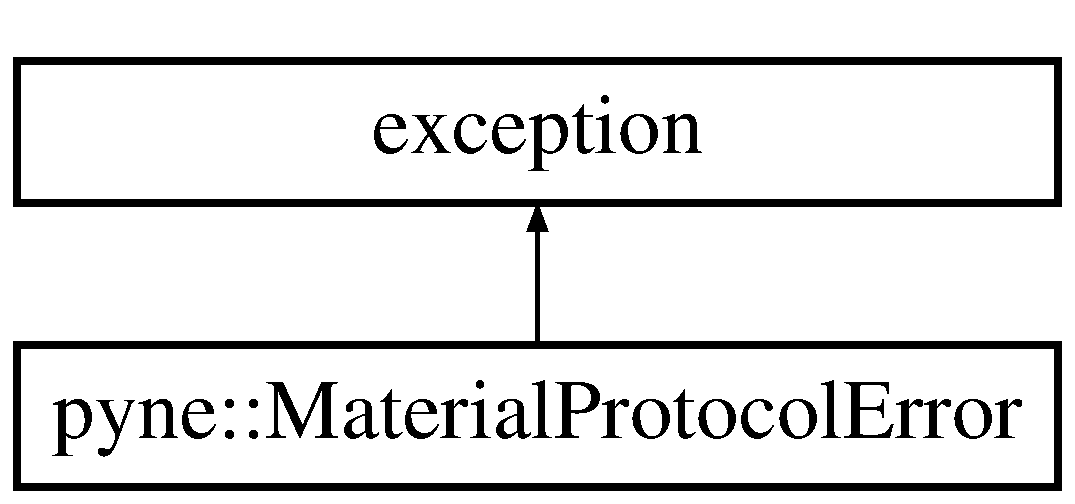
\includegraphics[height=2.000000cm]{classpyne_1_1_material_protocol_error}
\end{center}
\end{figure}


\subsection{Detailed Description}
Custom exception for invalid H\+D\+F5 protocol numbers. 

The documentation for this class was generated from the following file\+:\begin{DoxyCompactItemize}
\item 
/home/ubuntu/\+Documents/pyne.\+github.\+com/src/material.\+h\end{DoxyCompactItemize}

\hypertarget{structtracking__data__structures_1_1meshcell}{}\section{tracking\+\_\+data\+\_\+structures\+:\+:meshcell Type Reference}
\label{structtracking__data__structures_1_1meshcell}\index{tracking\+\_\+data\+\_\+structures\+::meshcell@{tracking\+\_\+data\+\_\+structures\+::meshcell}}
\subsection*{Public Attributes}
\begin{DoxyCompactItemize}
\item 
integer {\bfseries xind}\hypertarget{structtracking__data__structures_1_1meshcell_afd4a41c0924cdfa672043dff98383247}{}\label{structtracking__data__structures_1_1meshcell_afd4a41c0924cdfa672043dff98383247}

\item 
integer {\bfseries yind}\hypertarget{structtracking__data__structures_1_1meshcell_aaf221593bf60310472dfdcc78d6c2e79}{}\label{structtracking__data__structures_1_1meshcell_aaf221593bf60310472dfdcc78d6c2e79}

\item 
integer {\bfseries zind}\hypertarget{structtracking__data__structures_1_1meshcell_ae19a4af32e3f12bfa8042da05505aa6e}{}\label{structtracking__data__structures_1_1meshcell_ae19a4af32e3f12bfa8042da05505aa6e}

\item 
real(kind=pr), dimension(3, 8) {\bfseries corners}\hypertarget{structtracking__data__structures_1_1meshcell_a13fcf4021ce5a5d1579ffbff38aaf33d}{}\label{structtracking__data__structures_1_1meshcell_a13fcf4021ce5a5d1579ffbff38aaf33d}

\item 
real(kind=pr), dimension(3, 2, 12) {\bfseries edges}\hypertarget{structtracking__data__structures_1_1meshcell_a4edd8593d1bb0badbc5d723780d2c6c5}{}\label{structtracking__data__structures_1_1meshcell_a4edd8593d1bb0badbc5d723780d2c6c5}

\item 
real(kind=pr), dimension(3, 3, 6) {\bfseries faces}\hypertarget{structtracking__data__structures_1_1meshcell_a8b0a596007ab35b13961d9037d7b6e44}{}\label{structtracking__data__structures_1_1meshcell_a8b0a596007ab35b13961d9037d7b6e44}

\item 
real(kind=pr) {\bfseries volume}\hypertarget{structtracking__data__structures_1_1meshcell_a1a08090e934eae80b9b27f55c4ccaa00}{}\label{structtracking__data__structures_1_1meshcell_a1a08090e934eae80b9b27f55c4ccaa00}

\end{DoxyCompactItemize}


The documentation for this type was generated from the following file\+:\begin{DoxyCompactItemize}
\item 
/home/lucas/opt/gcc-\/6/pyne-\/dev/pyne/src/transport\+\_\+spatial\+\_\+methods/3d/trackstruct.\+f90\end{DoxyCompactItemize}

\hypertarget{structpyne_1_1ndsfpy}{}\section{pyne\+:\+:ndsfpy Struct Reference}
\label{structpyne_1_1ndsfpy}\index{pyne\+::ndsfpy@{pyne\+::ndsfpy}}


a struct matching the \textquotesingle{}/neutron/nds\+\_\+fission\+\_\+product\textquotesingle{} table in nuc\+\_\+data.\+h5  




{\ttfamily \#include $<$data.\+h$>$}

\subsection*{Public Attributes}
\begin{DoxyCompactItemize}
\item 
int \hyperlink{structpyne_1_1ndsfpy_ad2cb8c35a387624f95c5318f259834db}{from\+\_\+nuc}\hypertarget{structpyne_1_1ndsfpy_ad2cb8c35a387624f95c5318f259834db}{}\label{structpyne_1_1ndsfpy_ad2cb8c35a387624f95c5318f259834db}

\begin{DoxyCompactList}\small\item\em id of fissioning nuclide \end{DoxyCompactList}\item 
int \hyperlink{structpyne_1_1ndsfpy_aeabd96ca1b30be7381853ca0ccd75f31}{to\+\_\+nuc}\hypertarget{structpyne_1_1ndsfpy_aeabd96ca1b30be7381853ca0ccd75f31}{}\label{structpyne_1_1ndsfpy_aeabd96ca1b30be7381853ca0ccd75f31}

\begin{DoxyCompactList}\small\item\em id of fission product \end{DoxyCompactList}\item 
double \hyperlink{structpyne_1_1ndsfpy_a802ebba1436e6e7ca9595e77698310e8}{yield\+\_\+thermal}\hypertarget{structpyne_1_1ndsfpy_a802ebba1436e6e7ca9595e77698310e8}{}\label{structpyne_1_1ndsfpy_a802ebba1436e6e7ca9595e77698310e8}

\begin{DoxyCompactList}\small\item\em thermal yield \mbox{[}fraction\mbox{]} \end{DoxyCompactList}\item 
double \hyperlink{structpyne_1_1ndsfpy_affaf73e5d64d7e9e94f63c6807b7b17e}{yield\+\_\+thermal\+\_\+err}\hypertarget{structpyne_1_1ndsfpy_affaf73e5d64d7e9e94f63c6807b7b17e}{}\label{structpyne_1_1ndsfpy_affaf73e5d64d7e9e94f63c6807b7b17e}

\begin{DoxyCompactList}\small\item\em thermal yield error \mbox{[}fraction\mbox{]} \end{DoxyCompactList}\item 
double \hyperlink{structpyne_1_1ndsfpy_ae890b10d182d771d0837b24818040a25}{yield\+\_\+fast}\hypertarget{structpyne_1_1ndsfpy_ae890b10d182d771d0837b24818040a25}{}\label{structpyne_1_1ndsfpy_ae890b10d182d771d0837b24818040a25}

\begin{DoxyCompactList}\small\item\em fast yield \mbox{[}fraction\mbox{]} \end{DoxyCompactList}\item 
double \hyperlink{structpyne_1_1ndsfpy_a0e2478bc6cbf2317861727a88cb8370b}{yield\+\_\+fast\+\_\+err}\hypertarget{structpyne_1_1ndsfpy_a0e2478bc6cbf2317861727a88cb8370b}{}\label{structpyne_1_1ndsfpy_a0e2478bc6cbf2317861727a88cb8370b}

\begin{DoxyCompactList}\small\item\em fast yield error \mbox{[}fraction\mbox{]} \end{DoxyCompactList}\item 
double \hyperlink{structpyne_1_1ndsfpy_a5e67e99b97b5ca511ca39c6dcd4b186e}{yield\+\_\+14\+MeV}\hypertarget{structpyne_1_1ndsfpy_a5e67e99b97b5ca511ca39c6dcd4b186e}{}\label{structpyne_1_1ndsfpy_a5e67e99b97b5ca511ca39c6dcd4b186e}

\begin{DoxyCompactList}\small\item\em 14 MeV yield \mbox{[}fraction\mbox{]} \end{DoxyCompactList}\item 
double \hyperlink{structpyne_1_1ndsfpy_a1d24f4162fe242108b8032f76171d7e5}{yield\+\_\+14\+Me\+V\+\_\+err}\hypertarget{structpyne_1_1ndsfpy_a1d24f4162fe242108b8032f76171d7e5}{}\label{structpyne_1_1ndsfpy_a1d24f4162fe242108b8032f76171d7e5}

\begin{DoxyCompactList}\small\item\em 14 MeV yield error \mbox{[}fraction\mbox{]} \end{DoxyCompactList}\end{DoxyCompactItemize}


\subsection{Detailed Description}
a struct matching the \textquotesingle{}/neutron/nds\+\_\+fission\+\_\+product\textquotesingle{} table in nuc\+\_\+data.\+h5 

The documentation for this struct was generated from the following file\+:\begin{DoxyCompactItemize}
\item 
/home/lucas/opt/gcc-\/6/pyne-\/dev/pyne/src/\hyperlink{data_8h}{data.\+h}\end{DoxyCompactItemize}

\hypertarget{structpyne_1_1ndsfpysub}{}\section{pyne\+:\+:ndsfpysub Struct Reference}
\label{structpyne_1_1ndsfpysub}\index{pyne\+::ndsfpysub@{pyne\+::ndsfpysub}}


a struct for the nds data for fpyield  




{\ttfamily \#include $<$data.\+h$>$}

\subsection*{Public Attributes}
\begin{DoxyCompactItemize}
\item 
double \hyperlink{structpyne_1_1ndsfpysub_a83cf4a8733bb234e41c947a21a515cf0}{yield\+\_\+thermal}\hypertarget{structpyne_1_1ndsfpysub_a83cf4a8733bb234e41c947a21a515cf0}{}\label{structpyne_1_1ndsfpysub_a83cf4a8733bb234e41c947a21a515cf0}

\begin{DoxyCompactList}\small\item\em thermal yield \mbox{[}fraction\mbox{]} \end{DoxyCompactList}\item 
double \hyperlink{structpyne_1_1ndsfpysub_a8a95ca96e3cee6ef8a16dcbaf17ca6d3}{yield\+\_\+thermal\+\_\+err}\hypertarget{structpyne_1_1ndsfpysub_a8a95ca96e3cee6ef8a16dcbaf17ca6d3}{}\label{structpyne_1_1ndsfpysub_a8a95ca96e3cee6ef8a16dcbaf17ca6d3}

\begin{DoxyCompactList}\small\item\em thermal yield error \mbox{[}fraction\mbox{]} \end{DoxyCompactList}\item 
double \hyperlink{structpyne_1_1ndsfpysub_acc33c1cd93f9133c15024fa8d4b066dd}{yield\+\_\+fast}\hypertarget{structpyne_1_1ndsfpysub_acc33c1cd93f9133c15024fa8d4b066dd}{}\label{structpyne_1_1ndsfpysub_acc33c1cd93f9133c15024fa8d4b066dd}

\begin{DoxyCompactList}\small\item\em fast yield \mbox{[}fraction\mbox{]} \end{DoxyCompactList}\item 
double \hyperlink{structpyne_1_1ndsfpysub_aa7143b625fe8932ff159b3d9e0030b38}{yield\+\_\+fast\+\_\+err}\hypertarget{structpyne_1_1ndsfpysub_aa7143b625fe8932ff159b3d9e0030b38}{}\label{structpyne_1_1ndsfpysub_aa7143b625fe8932ff159b3d9e0030b38}

\begin{DoxyCompactList}\small\item\em fast yield error \mbox{[}fraction\mbox{]} \end{DoxyCompactList}\item 
double \hyperlink{structpyne_1_1ndsfpysub_afb3737be03fedddc6f54fa3a0e59f0e8}{yield\+\_\+14\+MeV}\hypertarget{structpyne_1_1ndsfpysub_afb3737be03fedddc6f54fa3a0e59f0e8}{}\label{structpyne_1_1ndsfpysub_afb3737be03fedddc6f54fa3a0e59f0e8}

\begin{DoxyCompactList}\small\item\em 14 MeV yield \mbox{[}fraction\mbox{]} \end{DoxyCompactList}\item 
double \hyperlink{structpyne_1_1ndsfpysub_a7bc2487245689a3f6a095f2254e66e99}{yield\+\_\+14\+Me\+V\+\_\+err}\hypertarget{structpyne_1_1ndsfpysub_a7bc2487245689a3f6a095f2254e66e99}{}\label{structpyne_1_1ndsfpysub_a7bc2487245689a3f6a095f2254e66e99}

\begin{DoxyCompactList}\small\item\em 14 MeV yield error \mbox{[}fraction\mbox{]} \end{DoxyCompactList}\end{DoxyCompactItemize}


\subsection{Detailed Description}
a struct for the nds data for fpyield 

The documentation for this struct was generated from the following file\+:\begin{DoxyCompactItemize}
\item 
/home/ubuntu/\+Desktop/new/pyne.\+github.\+com/src/\hyperlink{data_8h}{data.\+h}\end{DoxyCompactItemize}

\hypertarget{classpyne_1_1nucname_1_1_not_a_nuclide}{}\section{pyne\+:\+:nucname\+:\+:Not\+A\+Nuclide Class Reference}
\label{classpyne_1_1nucname_1_1_not_a_nuclide}\index{pyne\+::nucname\+::\+Not\+A\+Nuclide@{pyne\+::nucname\+::\+Not\+A\+Nuclide}}


{\ttfamily \#include $<$nucname.\+h$>$}

Inheritance diagram for pyne\+:\+:nucname\+:\+:Not\+A\+Nuclide\+:\begin{figure}[H]
\begin{center}
\leavevmode
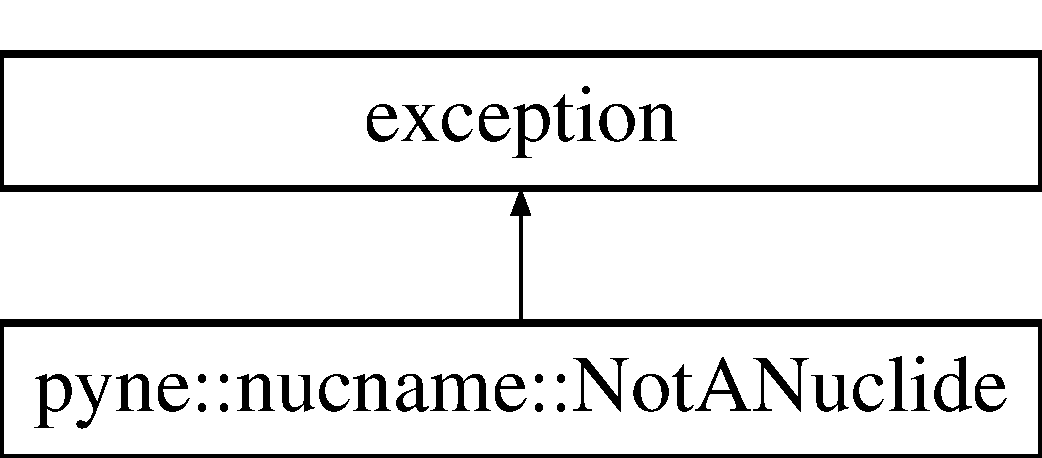
\includegraphics[height=2.000000cm]{classpyne_1_1nucname_1_1_not_a_nuclide}
\end{center}
\end{figure}
\subsection*{Public Member Functions}
\begin{DoxyCompactItemize}
\item 
\hyperlink{classpyne_1_1nucname_1_1_not_a_nuclide_ac1c10c25703f622788f475609fd5eed6}{Not\+A\+Nuclide} ()\hypertarget{classpyne_1_1nucname_1_1_not_a_nuclide_ac1c10c25703f622788f475609fd5eed6}{}\label{classpyne_1_1nucname_1_1_not_a_nuclide_ac1c10c25703f622788f475609fd5eed6}

\begin{DoxyCompactList}\small\item\em default constructor \end{DoxyCompactList}\item 
\hyperlink{classpyne_1_1nucname_1_1_not_a_nuclide_a2fd948fc4d3be06a456b30188944b88a}{$\sim$\+Not\+A\+Nuclide} ()  throw ()\hypertarget{classpyne_1_1nucname_1_1_not_a_nuclide_a2fd948fc4d3be06a456b30188944b88a}{}\label{classpyne_1_1nucname_1_1_not_a_nuclide_a2fd948fc4d3be06a456b30188944b88a}

\begin{DoxyCompactList}\small\item\em default destructor \end{DoxyCompactList}\item 
\hyperlink{classpyne_1_1nucname_1_1_not_a_nuclide_a32741575cb99d294d54f39bc4ca5e51c}{Not\+A\+Nuclide} (std\+::string wasptr, std\+::string nowptr)
\item 
\hyperlink{classpyne_1_1nucname_1_1_not_a_nuclide_a10f9f9c4be5b439f1dafd1450943252d}{Not\+A\+Nuclide} (std\+::string wasptr, int nowptr)
\item 
\hyperlink{classpyne_1_1nucname_1_1_not_a_nuclide_af8665194481f65e932cbd4244ee636ae}{Not\+A\+Nuclide} (int wasptr, std\+::string nowptr)
\item 
\hyperlink{classpyne_1_1nucname_1_1_not_a_nuclide_adbc9b62fa21ec1ab4957ca8a4569a8c6}{Not\+A\+Nuclide} (int wasptr, int nowptr)
\item 
virtual const char $\ast$ \hyperlink{classpyne_1_1nucname_1_1_not_a_nuclide_adb841d59149843b5b5718f5ccc47b4dc}{what} () const   throw ()
\end{DoxyCompactItemize}


\subsection{Detailed Description}
Custom expection for declaring that a value does not follow a recognizable nuclide naming convention. 

\subsection{Constructor \& Destructor Documentation}
\index{pyne\+::nucname\+::\+Not\+A\+Nuclide@{pyne\+::nucname\+::\+Not\+A\+Nuclide}!Not\+A\+Nuclide@{Not\+A\+Nuclide}}
\index{Not\+A\+Nuclide@{Not\+A\+Nuclide}!pyne\+::nucname\+::\+Not\+A\+Nuclide@{pyne\+::nucname\+::\+Not\+A\+Nuclide}}
\subsubsection[{\texorpdfstring{Not\+A\+Nuclide(std\+::string wasptr, std\+::string nowptr)}{NotANuclide(std::string wasptr, std::string nowptr)}}]{\setlength{\rightskip}{0pt plus 5cm}pyne\+::nucname\+::\+Not\+A\+Nuclide\+::\+Not\+A\+Nuclide (
\begin{DoxyParamCaption}
\item[{std\+::string}]{wasptr, }
\item[{std\+::string}]{nowptr}
\end{DoxyParamCaption}
)\hspace{0.3cm}{\ttfamily [inline]}}\hypertarget{classpyne_1_1nucname_1_1_not_a_nuclide_a32741575cb99d294d54f39bc4ca5e51c}{}\label{classpyne_1_1nucname_1_1_not_a_nuclide_a32741575cb99d294d54f39bc4ca5e51c}
Constructor given previous and current state of nulide name 
\begin{DoxyParams}{Parameters}
{\em wasptr} & Previous state, typically user input. \\
\hline
{\em nowptr} & Current state, as far as Py\+NE could get. \\
\hline
\end{DoxyParams}
\index{pyne\+::nucname\+::\+Not\+A\+Nuclide@{pyne\+::nucname\+::\+Not\+A\+Nuclide}!Not\+A\+Nuclide@{Not\+A\+Nuclide}}
\index{Not\+A\+Nuclide@{Not\+A\+Nuclide}!pyne\+::nucname\+::\+Not\+A\+Nuclide@{pyne\+::nucname\+::\+Not\+A\+Nuclide}}
\subsubsection[{\texorpdfstring{Not\+A\+Nuclide(std\+::string wasptr, int nowptr)}{NotANuclide(std::string wasptr, int nowptr)}}]{\setlength{\rightskip}{0pt plus 5cm}pyne\+::nucname\+::\+Not\+A\+Nuclide\+::\+Not\+A\+Nuclide (
\begin{DoxyParamCaption}
\item[{std\+::string}]{wasptr, }
\item[{int}]{nowptr}
\end{DoxyParamCaption}
)\hspace{0.3cm}{\ttfamily [inline]}}\hypertarget{classpyne_1_1nucname_1_1_not_a_nuclide_a10f9f9c4be5b439f1dafd1450943252d}{}\label{classpyne_1_1nucname_1_1_not_a_nuclide_a10f9f9c4be5b439f1dafd1450943252d}
Constructor given previous and current state of nulide name 
\begin{DoxyParams}{Parameters}
{\em wasptr} & Previous state, typically user input. \\
\hline
{\em nowptr} & Current state, as far as Py\+NE could get. \\
\hline
\end{DoxyParams}
\index{pyne\+::nucname\+::\+Not\+A\+Nuclide@{pyne\+::nucname\+::\+Not\+A\+Nuclide}!Not\+A\+Nuclide@{Not\+A\+Nuclide}}
\index{Not\+A\+Nuclide@{Not\+A\+Nuclide}!pyne\+::nucname\+::\+Not\+A\+Nuclide@{pyne\+::nucname\+::\+Not\+A\+Nuclide}}
\subsubsection[{\texorpdfstring{Not\+A\+Nuclide(int wasptr, std\+::string nowptr)}{NotANuclide(int wasptr, std::string nowptr)}}]{\setlength{\rightskip}{0pt plus 5cm}pyne\+::nucname\+::\+Not\+A\+Nuclide\+::\+Not\+A\+Nuclide (
\begin{DoxyParamCaption}
\item[{int}]{wasptr, }
\item[{std\+::string}]{nowptr}
\end{DoxyParamCaption}
)\hspace{0.3cm}{\ttfamily [inline]}}\hypertarget{classpyne_1_1nucname_1_1_not_a_nuclide_af8665194481f65e932cbd4244ee636ae}{}\label{classpyne_1_1nucname_1_1_not_a_nuclide_af8665194481f65e932cbd4244ee636ae}
Constructor given previous and current state of nulide name 
\begin{DoxyParams}{Parameters}
{\em wasptr} & Previous state, typically user input. \\
\hline
{\em nowptr} & Current state, as far as Py\+NE could get. \\
\hline
\end{DoxyParams}
\index{pyne\+::nucname\+::\+Not\+A\+Nuclide@{pyne\+::nucname\+::\+Not\+A\+Nuclide}!Not\+A\+Nuclide@{Not\+A\+Nuclide}}
\index{Not\+A\+Nuclide@{Not\+A\+Nuclide}!pyne\+::nucname\+::\+Not\+A\+Nuclide@{pyne\+::nucname\+::\+Not\+A\+Nuclide}}
\subsubsection[{\texorpdfstring{Not\+A\+Nuclide(int wasptr, int nowptr)}{NotANuclide(int wasptr, int nowptr)}}]{\setlength{\rightskip}{0pt plus 5cm}pyne\+::nucname\+::\+Not\+A\+Nuclide\+::\+Not\+A\+Nuclide (
\begin{DoxyParamCaption}
\item[{int}]{wasptr, }
\item[{int}]{nowptr}
\end{DoxyParamCaption}
)\hspace{0.3cm}{\ttfamily [inline]}}\hypertarget{classpyne_1_1nucname_1_1_not_a_nuclide_adbc9b62fa21ec1ab4957ca8a4569a8c6}{}\label{classpyne_1_1nucname_1_1_not_a_nuclide_adbc9b62fa21ec1ab4957ca8a4569a8c6}
Constructor given previous and current state of nulide name 
\begin{DoxyParams}{Parameters}
{\em wasptr} & Previous state, typically user input. \\
\hline
{\em nowptr} & Current state, as far as Py\+NE could get. \\
\hline
\end{DoxyParams}


\subsection{Member Function Documentation}
\index{pyne\+::nucname\+::\+Not\+A\+Nuclide@{pyne\+::nucname\+::\+Not\+A\+Nuclide}!what@{what}}
\index{what@{what}!pyne\+::nucname\+::\+Not\+A\+Nuclide@{pyne\+::nucname\+::\+Not\+A\+Nuclide}}
\subsubsection[{\texorpdfstring{what() const }{what() const }}]{\setlength{\rightskip}{0pt plus 5cm}virtual const char$\ast$ pyne\+::nucname\+::\+Not\+A\+Nuclide\+::what (
\begin{DoxyParamCaption}
{}
\end{DoxyParamCaption}
) const throw  ) \hspace{0.3cm}{\ttfamily [inline]}, {\ttfamily [virtual]}}\hypertarget{classpyne_1_1nucname_1_1_not_a_nuclide_adb841d59149843b5b5718f5ccc47b4dc}{}\label{classpyne_1_1nucname_1_1_not_a_nuclide_adb841d59149843b5b5718f5ccc47b4dc}
Generates an informational message for the exception \begin{DoxyReturn}{Returns}
The error string 
\end{DoxyReturn}


The documentation for this class was generated from the following file\+:\begin{DoxyCompactItemize}
\item 
/home/ubuntu/\+Desktop/new/pyne.\+github.\+com/src/nucname.\+h\end{DoxyCompactItemize}

\hypertarget{classpyne_1_1particle_1_1_not_a_particle}{}\section{pyne\+:\+:particle\+:\+:Not\+A\+Particle Class Reference}
\label{classpyne_1_1particle_1_1_not_a_particle}\index{pyne\+::particle\+::\+Not\+A\+Particle@{pyne\+::particle\+::\+Not\+A\+Particle}}


Custom excpeption for failed particle types.  




{\ttfamily \#include $<$particle.\+h$>$}

Inheritance diagram for pyne\+:\+:particle\+:\+:Not\+A\+Particle\+:\begin{figure}[H]
\begin{center}
\leavevmode
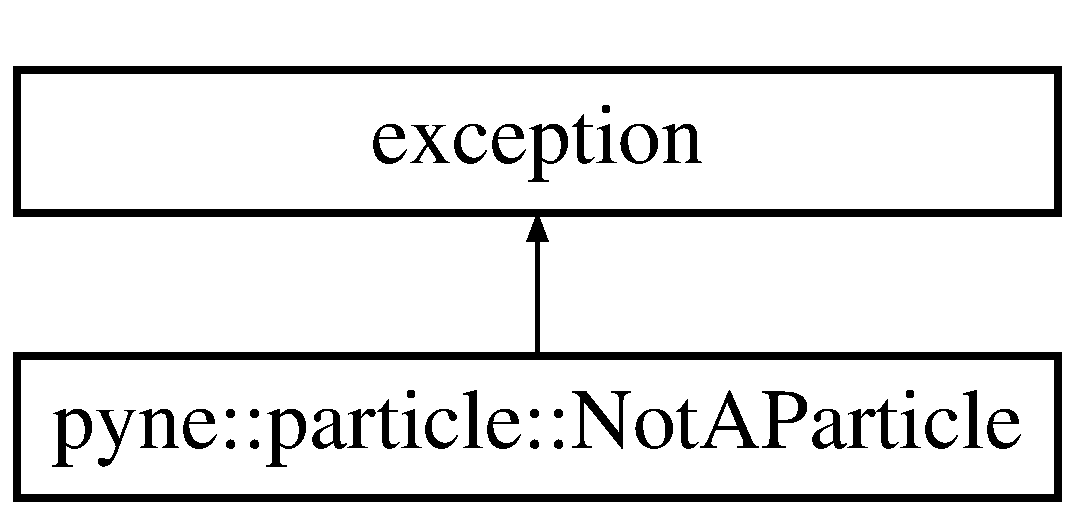
\includegraphics[height=2.000000cm]{classpyne_1_1particle_1_1_not_a_particle}
\end{center}
\end{figure}
\subsection*{Public Member Functions}
\begin{DoxyCompactItemize}
\item 
\hyperlink{classpyne_1_1particle_1_1_not_a_particle_af98a293003d5e5a570685c5985b7c501}{Not\+A\+Particle} ()\hypertarget{classpyne_1_1particle_1_1_not_a_particle_af98a293003d5e5a570685c5985b7c501}{}\label{classpyne_1_1particle_1_1_not_a_particle_af98a293003d5e5a570685c5985b7c501}

\begin{DoxyCompactList}\small\item\em Default constructor. \end{DoxyCompactList}\item 
\hyperlink{classpyne_1_1particle_1_1_not_a_particle_abe61e24b09e9846161bc264a1dc7978d}{$\sim$\+Not\+A\+Particle} ()  throw ()\hypertarget{classpyne_1_1particle_1_1_not_a_particle_abe61e24b09e9846161bc264a1dc7978d}{}\label{classpyne_1_1particle_1_1_not_a_particle_abe61e24b09e9846161bc264a1dc7978d}

\begin{DoxyCompactList}\small\item\em Default destructor. \end{DoxyCompactList}\item 
\hyperlink{classpyne_1_1particle_1_1_not_a_particle_a556fb7c90fc5e4c6ea1c394a86746fc9}{Not\+A\+Particle} (std\+::string particle\+\_\+name)
\item 
virtual const char $\ast$ \hyperlink{classpyne_1_1particle_1_1_not_a_particle_a70a50ceb3e0920b45acb4e779865b9db}{what} () const   throw ()\hypertarget{classpyne_1_1particle_1_1_not_a_particle_a70a50ceb3e0920b45acb4e779865b9db}{}\label{classpyne_1_1particle_1_1_not_a_particle_a70a50ceb3e0920b45acb4e779865b9db}

\begin{DoxyCompactList}\small\item\em raises error message \end{DoxyCompactList}\end{DoxyCompactItemize}


\subsection{Detailed Description}
Custom excpeption for failed particle types. 

\subsection{Constructor \& Destructor Documentation}
\index{pyne\+::particle\+::\+Not\+A\+Particle@{pyne\+::particle\+::\+Not\+A\+Particle}!Not\+A\+Particle@{Not\+A\+Particle}}
\index{Not\+A\+Particle@{Not\+A\+Particle}!pyne\+::particle\+::\+Not\+A\+Particle@{pyne\+::particle\+::\+Not\+A\+Particle}}
\subsubsection[{\texorpdfstring{Not\+A\+Particle(std\+::string particle\+\_\+name)}{NotAParticle(std::string particle_name)}}]{\setlength{\rightskip}{0pt plus 5cm}pyne\+::particle\+::\+Not\+A\+Particle\+::\+Not\+A\+Particle (
\begin{DoxyParamCaption}
\item[{std\+::string}]{particle\+\_\+name}
\end{DoxyParamCaption}
)\hspace{0.3cm}{\ttfamily [inline]}}\hypertarget{classpyne_1_1particle_1_1_not_a_particle_a556fb7c90fc5e4c6ea1c394a86746fc9}{}\label{classpyne_1_1particle_1_1_not_a_particle_a556fb7c90fc5e4c6ea1c394a86746fc9}
Constructor for raising the exception Spits out the particle name as input 

The documentation for this class was generated from the following file\+:\begin{DoxyCompactItemize}
\item 
/home/lucas/opt/gcc-\/6/pyne-\/dev/pyne/src/particle.\+h\end{DoxyCompactItemize}

\hypertarget{classpyne_1_1rxname_1_1_not_a_reaction}{}\section{pyne\+:\+:rxname\+:\+:Not\+A\+Reaction Class Reference}
\label{classpyne_1_1rxname_1_1_not_a_reaction}\index{pyne\+::rxname\+::\+Not\+A\+Reaction@{pyne\+::rxname\+::\+Not\+A\+Reaction}}


Custom exception for declaring a value not to be a valid reaction.  




{\ttfamily \#include $<$rxname.\+h$>$}

Inheritance diagram for pyne\+:\+:rxname\+:\+:Not\+A\+Reaction\+:\begin{figure}[H]
\begin{center}
\leavevmode
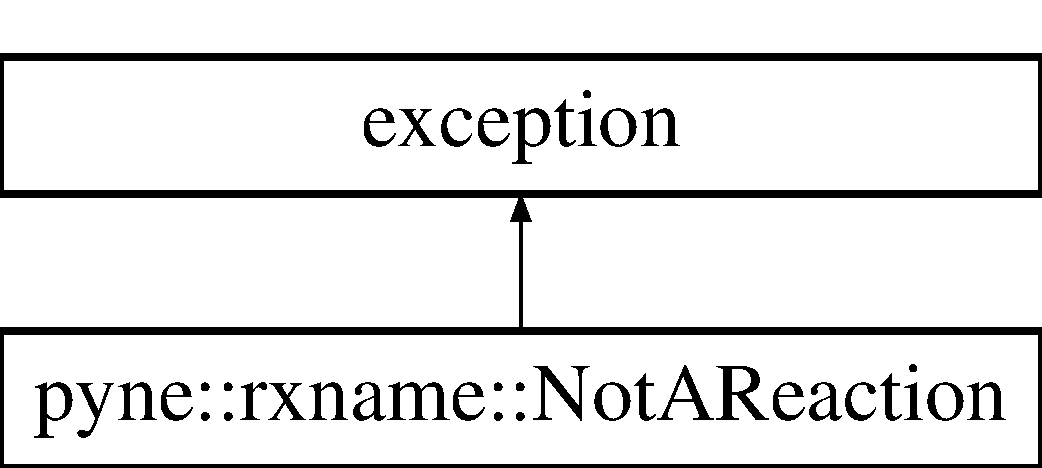
\includegraphics[height=2.000000cm]{classpyne_1_1rxname_1_1_not_a_reaction}
\end{center}
\end{figure}
\subsection*{Public Member Functions}
\begin{DoxyCompactItemize}
\item 
\hyperlink{classpyne_1_1rxname_1_1_not_a_reaction_abb889337afdab53c131adf5702fb16d0}{Not\+A\+Reaction} ()\hypertarget{classpyne_1_1rxname_1_1_not_a_reaction_abb889337afdab53c131adf5702fb16d0}{}\label{classpyne_1_1rxname_1_1_not_a_reaction_abb889337afdab53c131adf5702fb16d0}

\begin{DoxyCompactList}\small\item\em default constructor \end{DoxyCompactList}\item 
\hyperlink{classpyne_1_1rxname_1_1_not_a_reaction_a2a34cc0de45875c17c004acff20dc535}{$\sim$\+Not\+A\+Reaction} ()  throw ()\hypertarget{classpyne_1_1rxname_1_1_not_a_reaction_a2a34cc0de45875c17c004acff20dc535}{}\label{classpyne_1_1rxname_1_1_not_a_reaction_a2a34cc0de45875c17c004acff20dc535}

\begin{DoxyCompactList}\small\item\em default destructor \end{DoxyCompactList}\item 
\hyperlink{classpyne_1_1rxname_1_1_not_a_reaction_a64f23630722811847d030ae0358f959f}{Not\+A\+Reaction} (std\+::string wasptr, std\+::string nowptr)
\item 
\hyperlink{classpyne_1_1rxname_1_1_not_a_reaction_a32de94daecf33a00055c8ac7ada718d7}{Not\+A\+Reaction} (std\+::string wasptr, int nowptr)
\item 
\hyperlink{classpyne_1_1rxname_1_1_not_a_reaction_a828c48bf08dd96121ec83c6cced3063b}{Not\+A\+Reaction} (int wasptr, std\+::string nowptr)
\item 
\hyperlink{classpyne_1_1rxname_1_1_not_a_reaction_a8d16f260eab4fbbc7a5a14b48ce5580d}{Not\+A\+Reaction} (int wasptr, int nowptr)
\item 
\hyperlink{classpyne_1_1rxname_1_1_not_a_reaction_a9f3cea1e2ffd856bd3111569482244d2}{Not\+A\+Reaction} (std\+::string wasptr, unsigned int nowptr)
\item 
\hyperlink{classpyne_1_1rxname_1_1_not_a_reaction_ab5ff27c0ce93ac29da63ab32e7fa44e3}{Not\+A\+Reaction} (unsigned int wasptr, std\+::string nowptr)
\item 
\hyperlink{classpyne_1_1rxname_1_1_not_a_reaction_a7e0b63801e38b5d2c59edd635817fb80}{Not\+A\+Reaction} (unsigned int wasptr, unsigned int nowptr)
\item 
virtual const char $\ast$ \hyperlink{classpyne_1_1rxname_1_1_not_a_reaction_a82bd7ddf78f0065338ec546dfacf5b45}{what} () const   throw ()\hypertarget{classpyne_1_1rxname_1_1_not_a_reaction_a82bd7ddf78f0065338ec546dfacf5b45}{}\label{classpyne_1_1rxname_1_1_not_a_reaction_a82bd7ddf78f0065338ec546dfacf5b45}

\begin{DoxyCompactList}\small\item\em Returns a helpful error message containing prior and current reaction state. \end{DoxyCompactList}\end{DoxyCompactItemize}


\subsection{Detailed Description}
Custom exception for declaring a value not to be a valid reaction. 

\subsection{Constructor \& Destructor Documentation}
\index{pyne\+::rxname\+::\+Not\+A\+Reaction@{pyne\+::rxname\+::\+Not\+A\+Reaction}!Not\+A\+Reaction@{Not\+A\+Reaction}}
\index{Not\+A\+Reaction@{Not\+A\+Reaction}!pyne\+::rxname\+::\+Not\+A\+Reaction@{pyne\+::rxname\+::\+Not\+A\+Reaction}}
\subsubsection[{\texorpdfstring{Not\+A\+Reaction(std\+::string wasptr, std\+::string nowptr)}{NotAReaction(std::string wasptr, std::string nowptr)}}]{\setlength{\rightskip}{0pt plus 5cm}pyne\+::rxname\+::\+Not\+A\+Reaction\+::\+Not\+A\+Reaction (
\begin{DoxyParamCaption}
\item[{std\+::string}]{wasptr, }
\item[{std\+::string}]{nowptr}
\end{DoxyParamCaption}
)\hspace{0.3cm}{\ttfamily [inline]}}\hypertarget{classpyne_1_1rxname_1_1_not_a_reaction_a64f23630722811847d030ae0358f959f}{}\label{classpyne_1_1rxname_1_1_not_a_reaction_a64f23630722811847d030ae0358f959f}
Constructor using original reaction ({\itshape wasptr}) and the eventual state that Py\+NE calculated ({\itshape nowptr}). \index{pyne\+::rxname\+::\+Not\+A\+Reaction@{pyne\+::rxname\+::\+Not\+A\+Reaction}!Not\+A\+Reaction@{Not\+A\+Reaction}}
\index{Not\+A\+Reaction@{Not\+A\+Reaction}!pyne\+::rxname\+::\+Not\+A\+Reaction@{pyne\+::rxname\+::\+Not\+A\+Reaction}}
\subsubsection[{\texorpdfstring{Not\+A\+Reaction(std\+::string wasptr, int nowptr)}{NotAReaction(std::string wasptr, int nowptr)}}]{\setlength{\rightskip}{0pt plus 5cm}pyne\+::rxname\+::\+Not\+A\+Reaction\+::\+Not\+A\+Reaction (
\begin{DoxyParamCaption}
\item[{std\+::string}]{wasptr, }
\item[{int}]{nowptr}
\end{DoxyParamCaption}
)\hspace{0.3cm}{\ttfamily [inline]}}\hypertarget{classpyne_1_1rxname_1_1_not_a_reaction_a32de94daecf33a00055c8ac7ada718d7}{}\label{classpyne_1_1rxname_1_1_not_a_reaction_a32de94daecf33a00055c8ac7ada718d7}
Constructor using original reaction ({\itshape wasptr}) and the eventual state that Py\+NE calculated ({\itshape nowptr}). \index{pyne\+::rxname\+::\+Not\+A\+Reaction@{pyne\+::rxname\+::\+Not\+A\+Reaction}!Not\+A\+Reaction@{Not\+A\+Reaction}}
\index{Not\+A\+Reaction@{Not\+A\+Reaction}!pyne\+::rxname\+::\+Not\+A\+Reaction@{pyne\+::rxname\+::\+Not\+A\+Reaction}}
\subsubsection[{\texorpdfstring{Not\+A\+Reaction(int wasptr, std\+::string nowptr)}{NotAReaction(int wasptr, std::string nowptr)}}]{\setlength{\rightskip}{0pt plus 5cm}pyne\+::rxname\+::\+Not\+A\+Reaction\+::\+Not\+A\+Reaction (
\begin{DoxyParamCaption}
\item[{int}]{wasptr, }
\item[{std\+::string}]{nowptr}
\end{DoxyParamCaption}
)\hspace{0.3cm}{\ttfamily [inline]}}\hypertarget{classpyne_1_1rxname_1_1_not_a_reaction_a828c48bf08dd96121ec83c6cced3063b}{}\label{classpyne_1_1rxname_1_1_not_a_reaction_a828c48bf08dd96121ec83c6cced3063b}
Constructor using original reaction ({\itshape wasptr}) and the eventual state that Py\+NE calculated ({\itshape nowptr}). \index{pyne\+::rxname\+::\+Not\+A\+Reaction@{pyne\+::rxname\+::\+Not\+A\+Reaction}!Not\+A\+Reaction@{Not\+A\+Reaction}}
\index{Not\+A\+Reaction@{Not\+A\+Reaction}!pyne\+::rxname\+::\+Not\+A\+Reaction@{pyne\+::rxname\+::\+Not\+A\+Reaction}}
\subsubsection[{\texorpdfstring{Not\+A\+Reaction(int wasptr, int nowptr)}{NotAReaction(int wasptr, int nowptr)}}]{\setlength{\rightskip}{0pt plus 5cm}pyne\+::rxname\+::\+Not\+A\+Reaction\+::\+Not\+A\+Reaction (
\begin{DoxyParamCaption}
\item[{int}]{wasptr, }
\item[{int}]{nowptr}
\end{DoxyParamCaption}
)\hspace{0.3cm}{\ttfamily [inline]}}\hypertarget{classpyne_1_1rxname_1_1_not_a_reaction_a8d16f260eab4fbbc7a5a14b48ce5580d}{}\label{classpyne_1_1rxname_1_1_not_a_reaction_a8d16f260eab4fbbc7a5a14b48ce5580d}
Constructor using original reaction ({\itshape wasptr}) and the eventual state that Py\+NE calculated ({\itshape nowptr}). \index{pyne\+::rxname\+::\+Not\+A\+Reaction@{pyne\+::rxname\+::\+Not\+A\+Reaction}!Not\+A\+Reaction@{Not\+A\+Reaction}}
\index{Not\+A\+Reaction@{Not\+A\+Reaction}!pyne\+::rxname\+::\+Not\+A\+Reaction@{pyne\+::rxname\+::\+Not\+A\+Reaction}}
\subsubsection[{\texorpdfstring{Not\+A\+Reaction(std\+::string wasptr, unsigned int nowptr)}{NotAReaction(std::string wasptr, unsigned int nowptr)}}]{\setlength{\rightskip}{0pt plus 5cm}pyne\+::rxname\+::\+Not\+A\+Reaction\+::\+Not\+A\+Reaction (
\begin{DoxyParamCaption}
\item[{std\+::string}]{wasptr, }
\item[{unsigned int}]{nowptr}
\end{DoxyParamCaption}
)\hspace{0.3cm}{\ttfamily [inline]}}\hypertarget{classpyne_1_1rxname_1_1_not_a_reaction_a9f3cea1e2ffd856bd3111569482244d2}{}\label{classpyne_1_1rxname_1_1_not_a_reaction_a9f3cea1e2ffd856bd3111569482244d2}
Constructor using original reaction ({\itshape wasptr}) and the eventual state that Py\+NE calculated ({\itshape nowptr}). \index{pyne\+::rxname\+::\+Not\+A\+Reaction@{pyne\+::rxname\+::\+Not\+A\+Reaction}!Not\+A\+Reaction@{Not\+A\+Reaction}}
\index{Not\+A\+Reaction@{Not\+A\+Reaction}!pyne\+::rxname\+::\+Not\+A\+Reaction@{pyne\+::rxname\+::\+Not\+A\+Reaction}}
\subsubsection[{\texorpdfstring{Not\+A\+Reaction(unsigned int wasptr, std\+::string nowptr)}{NotAReaction(unsigned int wasptr, std::string nowptr)}}]{\setlength{\rightskip}{0pt plus 5cm}pyne\+::rxname\+::\+Not\+A\+Reaction\+::\+Not\+A\+Reaction (
\begin{DoxyParamCaption}
\item[{unsigned int}]{wasptr, }
\item[{std\+::string}]{nowptr}
\end{DoxyParamCaption}
)\hspace{0.3cm}{\ttfamily [inline]}}\hypertarget{classpyne_1_1rxname_1_1_not_a_reaction_ab5ff27c0ce93ac29da63ab32e7fa44e3}{}\label{classpyne_1_1rxname_1_1_not_a_reaction_ab5ff27c0ce93ac29da63ab32e7fa44e3}
Constructor using original reaction ({\itshape wasptr}) and the eventual state that Py\+NE calculated ({\itshape nowptr}). \index{pyne\+::rxname\+::\+Not\+A\+Reaction@{pyne\+::rxname\+::\+Not\+A\+Reaction}!Not\+A\+Reaction@{Not\+A\+Reaction}}
\index{Not\+A\+Reaction@{Not\+A\+Reaction}!pyne\+::rxname\+::\+Not\+A\+Reaction@{pyne\+::rxname\+::\+Not\+A\+Reaction}}
\subsubsection[{\texorpdfstring{Not\+A\+Reaction(unsigned int wasptr, unsigned int nowptr)}{NotAReaction(unsigned int wasptr, unsigned int nowptr)}}]{\setlength{\rightskip}{0pt plus 5cm}pyne\+::rxname\+::\+Not\+A\+Reaction\+::\+Not\+A\+Reaction (
\begin{DoxyParamCaption}
\item[{unsigned int}]{wasptr, }
\item[{unsigned int}]{nowptr}
\end{DoxyParamCaption}
)\hspace{0.3cm}{\ttfamily [inline]}}\hypertarget{classpyne_1_1rxname_1_1_not_a_reaction_a7e0b63801e38b5d2c59edd635817fb80}{}\label{classpyne_1_1rxname_1_1_not_a_reaction_a7e0b63801e38b5d2c59edd635817fb80}
Constructor using original reaction ({\itshape wasptr}) and the eventual state that Py\+NE calculated ({\itshape nowptr}). 

The documentation for this class was generated from the following file\+:\begin{DoxyCompactItemize}
\item 
/home/ubuntu/\+Documents/pyne.\+github.\+com/src/rxname.\+h\end{DoxyCompactItemize}

\hypertarget{classh5wrap_1_1_path_not_found}{}\section{h5wrap\+:\+:Path\+Not\+Found Class Reference}
\label{classh5wrap_1_1_path_not_found}\index{h5wrap\+::\+Path\+Not\+Found@{h5wrap\+::\+Path\+Not\+Found}}


Custom exception for when a path is not found in an H\+D\+F5 file.  




{\ttfamily \#include $<$h5wrap.\+h$>$}

Inheritance diagram for h5wrap\+:\+:Path\+Not\+Found\+:\begin{figure}[H]
\begin{center}
\leavevmode
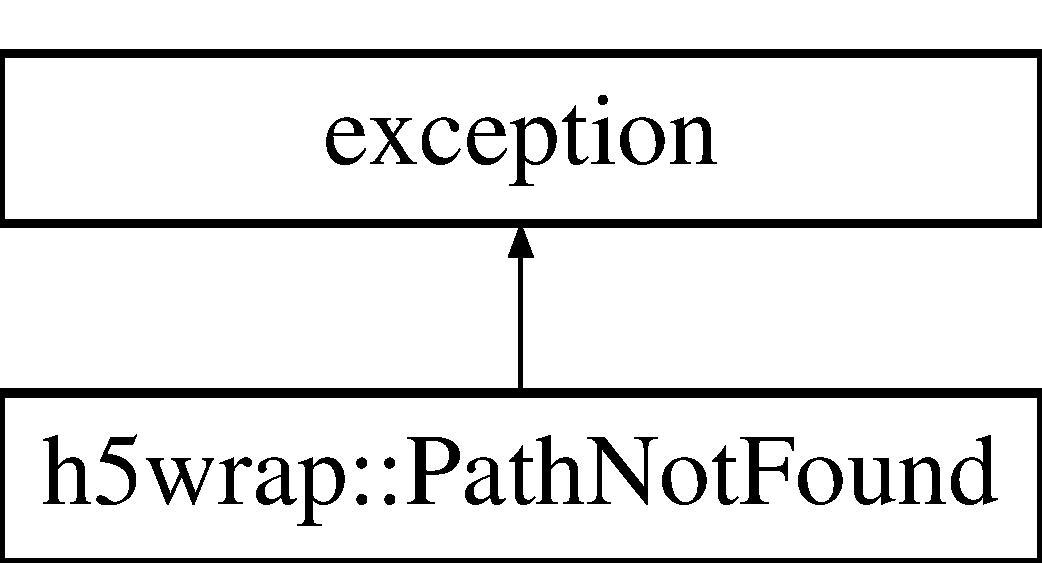
\includegraphics[height=2.000000cm]{classh5wrap_1_1_path_not_found}
\end{center}
\end{figure}
\subsection*{Public Member Functions}
\begin{DoxyCompactItemize}
\item 
\hyperlink{classh5wrap_1_1_path_not_found_a7b05229fb4f02920732f22622af1f08e}{Path\+Not\+Found} ()\hypertarget{classh5wrap_1_1_path_not_found_a7b05229fb4f02920732f22622af1f08e}{}\label{classh5wrap_1_1_path_not_found_a7b05229fb4f02920732f22622af1f08e}

\begin{DoxyCompactList}\small\item\em default constructor \end{DoxyCompactList}\item 
\hyperlink{classh5wrap_1_1_path_not_found_acf9696ccdfb4a4c63454dbfc1dcde060}{$\sim$\+Path\+Not\+Found} ()  throw ()\hypertarget{classh5wrap_1_1_path_not_found_acf9696ccdfb4a4c63454dbfc1dcde060}{}\label{classh5wrap_1_1_path_not_found_acf9696ccdfb4a4c63454dbfc1dcde060}

\begin{DoxyCompactList}\small\item\em default destructor \end{DoxyCompactList}\item 
\hyperlink{classh5wrap_1_1_path_not_found_aaedd26703acced17206eb8dabd4c5274}{Path\+Not\+Found} (std\+::string fname, std\+::string pname)\hypertarget{classh5wrap_1_1_path_not_found_aaedd26703acced17206eb8dabd4c5274}{}\label{classh5wrap_1_1_path_not_found_aaedd26703acced17206eb8dabd4c5274}

\begin{DoxyCompactList}\small\item\em constructor with the filename and the pathname \end{DoxyCompactList}\item 
virtual const char $\ast$ \hyperlink{classh5wrap_1_1_path_not_found_ad454d14e0f9f44f4357a5c33a7017b88}{what} () const   throw ()\hypertarget{classh5wrap_1_1_path_not_found_ad454d14e0f9f44f4357a5c33a7017b88}{}\label{classh5wrap_1_1_path_not_found_ad454d14e0f9f44f4357a5c33a7017b88}

\begin{DoxyCompactList}\small\item\em helpful error message that includes the filename and the pathname \end{DoxyCompactList}\end{DoxyCompactItemize}


\subsection{Detailed Description}
Custom exception for when a path is not found in an H\+D\+F5 file. 

The documentation for this class was generated from the following file\+:\begin{DoxyCompactItemize}
\item 
/home/ubuntu/\+Documents/pyne.\+github.\+com/src/\hyperlink{h5wrap_8h}{h5wrap.\+h}\end{DoxyCompactItemize}

\hypertarget{structsct__module_1_1polyhedron}{}\section{sct\+\_\+module\+:\+:polyhedron Type Reference}
\label{structsct__module_1_1polyhedron}\index{sct\+\_\+module\+::polyhedron@{sct\+\_\+module\+::polyhedron}}
\subsection*{Public Attributes}
\begin{DoxyCompactItemize}
\item 
integer, dimension(3) {\bfseries indx}\hypertarget{structsct__module_1_1polyhedron_a0a9f5f4cc18647a9ebeb2318bc83dfa7}{}\label{structsct__module_1_1polyhedron_a0a9f5f4cc18647a9ebeb2318bc83dfa7}

\item 
real(kind=dp) {\bfseries volume}\hypertarget{structsct__module_1_1polyhedron_a20eae3d573880fd36935c35d3b1d6c75}{}\label{structsct__module_1_1polyhedron_a20eae3d573880fd36935c35d3b1d6c75}

\item 
real(kind=dp), dimension(-\/3\+:3) {\bfseries area}\hypertarget{structsct__module_1_1polyhedron_aa39269bf2d196995f86f0b365b7c46dd}{}\label{structsct__module_1_1polyhedron_aa39269bf2d196995f86f0b365b7c46dd}

\item 
integer(kind=1), dimension(-\/3\+:3) {\bfseries area\+\_\+exist}\hypertarget{structsct__module_1_1polyhedron_a4d8b6322e32640812e3c917645febc0b}{}\label{structsct__module_1_1polyhedron_a4d8b6322e32640812e3c917645febc0b}

\end{DoxyCompactItemize}


The documentation for this type was generated from the following file\+:\begin{DoxyCompactItemize}
\item 
/home/lucas/opt/gcc-\/6/pyne-\/dev/pyne/src/transport\+\_\+spatial\+\_\+methods/3d/sct\+\_\+module.\+f90\end{DoxyCompactItemize}

\hypertarget{structpyne_1_1q__val__data}{}\section{pyne\+:\+:q\+\_\+val\+\_\+data Struct Reference}
\label{structpyne_1_1q__val__data}\index{pyne\+::q\+\_\+val\+\_\+data@{pyne\+::q\+\_\+val\+\_\+data}}


a struct matching the q\+\_\+value table in nuc\+\_\+data.\+h5.  




{\ttfamily \#include $<$data.\+h$>$}

\subsection*{Public Attributes}
\begin{DoxyCompactItemize}
\item 
int \hyperlink{structpyne_1_1q__val__data_a39dbf1ad0347f0f68f09c94a9ff9157f}{nuc}\hypertarget{structpyne_1_1q__val__data_a39dbf1ad0347f0f68f09c94a9ff9157f}{}\label{structpyne_1_1q__val__data_a39dbf1ad0347f0f68f09c94a9ff9157f}

\begin{DoxyCompactList}\small\item\em nuclide in id form \end{DoxyCompactList}\item 
double \hyperlink{structpyne_1_1q__val__data_a8016ec428535fddb8cba5005511d4a8a}{q\+\_\+val}\hypertarget{structpyne_1_1q__val__data_a8016ec428535fddb8cba5005511d4a8a}{}\label{structpyne_1_1q__val__data_a8016ec428535fddb8cba5005511d4a8a}

\begin{DoxyCompactList}\small\item\em nuclide q\+\_\+value \mbox{[}Me\+V/fission\mbox{]} \end{DoxyCompactList}\item 
double \hyperlink{structpyne_1_1q__val__data_a5d47c172a924715d567a1b6119e20830}{gamma\+\_\+frac}\hypertarget{structpyne_1_1q__val__data_a5d47c172a924715d567a1b6119e20830}{}\label{structpyne_1_1q__val__data_a5d47c172a924715d567a1b6119e20830}

\begin{DoxyCompactList}\small\item\em fraction of q that comes from gammas \end{DoxyCompactList}\end{DoxyCompactItemize}


\subsection{Detailed Description}
a struct matching the q\+\_\+value table in nuc\+\_\+data.\+h5. 

The documentation for this struct was generated from the following file\+:\begin{DoxyCompactItemize}
\item 
/home/ubuntu/\+Desktop/new/pyne.\+github.\+com/src/\hyperlink{data_8h}{data.\+h}\end{DoxyCompactItemize}

\hypertarget{classpyne_1_1ray__buffers}{}\section{pyne\+:\+:ray\+\_\+buffers Class Reference}
\label{classpyne_1_1ray__buffers}\index{pyne\+::ray\+\_\+buffers@{pyne\+::ray\+\_\+buffers}}
\subsection*{Public Attributes}
\begin{DoxyCompactItemize}
\item 
Dag\+M\+C\+::\+Ray\+History {\bfseries history}\hypertarget{classpyne_1_1ray__buffers_adb3331dbf290b1c6d44c37931a917a7e}{}\label{classpyne_1_1ray__buffers_adb3331dbf290b1c6d44c37931a917a7e}

\item 
std\+::vector$<$ Entity\+Handle $>$ {\bfseries surfs}\hypertarget{classpyne_1_1ray__buffers_ac2a784c86703f7253861ceaa73ba5e6b}{}\label{classpyne_1_1ray__buffers_ac2a784c86703f7253861ceaa73ba5e6b}

\item 
std\+::vector$<$ double $>$ {\bfseries dists}\hypertarget{classpyne_1_1ray__buffers_a2904cd95dd5c1cb04ca796cf025bced1}{}\label{classpyne_1_1ray__buffers_a2904cd95dd5c1cb04ca796cf025bced1}

\item 
std\+::vector$<$ Entity\+Handle $>$ {\bfseries vols}\hypertarget{classpyne_1_1ray__buffers_a2d059fcf9432e03b28eade60308b2498}{}\label{classpyne_1_1ray__buffers_a2d059fcf9432e03b28eade60308b2498}

\end{DoxyCompactItemize}


The documentation for this class was generated from the following file\+:\begin{DoxyCompactItemize}
\item 
/home/ubuntu/\+Desktop/new/pyne.\+github.\+com/src/dagmc\+\_\+bridge.\+cpp\end{DoxyCompactItemize}

\hypertarget{classpyne_1_1_sampler}{}\section{pyne\+:\+:Sampler Class Reference}
\label{classpyne_1_1_sampler}\index{pyne\+::\+Sampler@{pyne\+::\+Sampler}}


Mesh based Monte Carlo source sampling.  




{\ttfamily \#include $<$source\+\_\+sampling.\+h$>$}

\subsection*{Public Member Functions}
\begin{DoxyCompactItemize}
\item 
\hyperlink{classpyne_1_1_sampler_a57e096205922e6a221f2185a9849c5ed}{Sampler} (std\+::string filename, std\+::string src\+\_\+tag\+\_\+name, std\+::vector$<$ double $>$ e\+\_\+bounds, bool uniform)
\item 
\hyperlink{classpyne_1_1_sampler_a058411845da467ff7421956ba076ac31}{Sampler} (std\+::string filename, std\+::string src\+\_\+tag\+\_\+name, std\+::vector$<$ double $>$ e\+\_\+bounds, std\+::string bias\+\_\+tag\+\_\+name)
\item 
std\+::vector$<$ double $>$ \hyperlink{classpyne_1_1_sampler_aa5d177ee74199617fc08e4a7a7686e8f}{particle\+\_\+birth} (std\+::vector$<$ double $>$ rands)
\end{DoxyCompactItemize}


\subsection{Detailed Description}
Mesh based Monte Carlo source sampling. 

\subsection{Constructor \& Destructor Documentation}
\index{pyne\+::\+Sampler@{pyne\+::\+Sampler}!Sampler@{Sampler}}
\index{Sampler@{Sampler}!pyne\+::\+Sampler@{pyne\+::\+Sampler}}
\subsubsection[{\texorpdfstring{Sampler(std\+::string filename, std\+::string src\+\_\+tag\+\_\+name, std\+::vector$<$ double $>$ e\+\_\+bounds, bool uniform)}{Sampler(std::string filename, std::string src_tag_name, std::vector< double > e_bounds, bool uniform)}}]{\setlength{\rightskip}{0pt plus 5cm}pyne\+::\+Sampler\+::\+Sampler (
\begin{DoxyParamCaption}
\item[{std\+::string}]{filename, }
\item[{std\+::string}]{src\+\_\+tag\+\_\+name, }
\item[{std\+::vector$<$ double $>$}]{e\+\_\+bounds, }
\item[{bool}]{uniform}
\end{DoxyParamCaption}
)}\hypertarget{classpyne_1_1_sampler_a57e096205922e6a221f2185a9849c5ed}{}\label{classpyne_1_1_sampler_a57e096205922e6a221f2185a9849c5ed}
Constuctor for analog and uniform sampling 
\begin{DoxyParams}{Parameters}
{\em filename} & The path to the M\+O\+AB mesh (.h5m) file \\
\hline
{\em src\+\_\+tag\+\_\+name} & The name of the tag that describes the unbiased source density distribution. \\
\hline
{\em e\+\_\+bounds} & The energy boundaries, note there are N + 1 energy bounds for N energy groups \\
\hline
{\em uniform} & If false, analog sampling is used. If true, uniform sampling is used. \\
\hline
\end{DoxyParams}
\index{pyne\+::\+Sampler@{pyne\+::\+Sampler}!Sampler@{Sampler}}
\index{Sampler@{Sampler}!pyne\+::\+Sampler@{pyne\+::\+Sampler}}
\subsubsection[{\texorpdfstring{Sampler(std\+::string filename, std\+::string src\+\_\+tag\+\_\+name, std\+::vector$<$ double $>$ e\+\_\+bounds, std\+::string bias\+\_\+tag\+\_\+name)}{Sampler(std::string filename, std::string src_tag_name, std::vector< double > e_bounds, std::string bias_tag_name)}}]{\setlength{\rightskip}{0pt plus 5cm}pyne\+::\+Sampler\+::\+Sampler (
\begin{DoxyParamCaption}
\item[{std\+::string}]{filename, }
\item[{std\+::string}]{src\+\_\+tag\+\_\+name, }
\item[{std\+::vector$<$ double $>$}]{e\+\_\+bounds, }
\item[{std\+::string}]{bias\+\_\+tag\+\_\+name}
\end{DoxyParamCaption}
)}\hypertarget{classpyne_1_1_sampler_a058411845da467ff7421956ba076ac31}{}\label{classpyne_1_1_sampler_a058411845da467ff7421956ba076ac31}
Constuctor for analog and uniform sampling 
\begin{DoxyParams}{Parameters}
{\em filename} & The path to the M\+O\+AB mesh (.h5m) file \\
\hline
{\em src\+\_\+tag\+\_\+name} & The name of the tag with the unbiased source density distribution. \\
\hline
{\em e\+\_\+bounds} & The energy boundaries, note there are N + 1 energy bounds for N energy groups \\
\hline
{\em bias\+\_\+tag\+\_\+name} & The name of the tag describing the biased source density distribution. The tag must have the same number of energy groups as $<$src\+\_\+tag\+\_\+name$>$ or 1. If 1 (i.\+e. spatial biasing only), all energy groups within a mesh volume element are sampled equally. \\
\hline
\end{DoxyParams}


\subsection{Member Function Documentation}
\index{pyne\+::\+Sampler@{pyne\+::\+Sampler}!particle\+\_\+birth@{particle\+\_\+birth}}
\index{particle\+\_\+birth@{particle\+\_\+birth}!pyne\+::\+Sampler@{pyne\+::\+Sampler}}
\subsubsection[{\texorpdfstring{particle\+\_\+birth(std\+::vector$<$ double $>$ rands)}{particle_birth(std::vector< double > rands)}}]{\setlength{\rightskip}{0pt plus 5cm}std\+::vector$<$ double $>$ pyne\+::\+Sampler\+::particle\+\_\+birth (
\begin{DoxyParamCaption}
\item[{std\+::vector$<$ double $>$}]{rands}
\end{DoxyParamCaption}
)}\hypertarget{classpyne_1_1_sampler_aa5d177ee74199617fc08e4a7a7686e8f}{}\label{classpyne_1_1_sampler_aa5d177ee74199617fc08e4a7a7686e8f}
Samples particle birth parameters 
\begin{DoxyParams}{Parameters}
{\em rands} & Six pseudo-\/random numbers in range \mbox{[}0, 1\mbox{]}. \\
\hline
\end{DoxyParams}
\begin{DoxyReturn}{Returns}
A vector containing the x position, y, position, z, point, energy and weight of a particle (in that order). 
\end{DoxyReturn}


The documentation for this class was generated from the following files\+:\begin{DoxyCompactItemize}
\item 
/home/lucas/opt/gcc-\/6/pyne-\/dev/pyne/src/\hyperlink{source__sampling_8h}{source\+\_\+sampling.\+h}\item 
/home/lucas/opt/gcc-\/6/pyne-\/dev/pyne/src/source\+\_\+sampling.\+cpp\end{DoxyCompactItemize}

\hypertarget{structpyne_1_1scattering__lengths}{}\section{pyne\+:\+:scattering\+\_\+lengths Struct Reference}
\label{structpyne_1_1scattering__lengths}\index{pyne\+::scattering\+\_\+lengths@{pyne\+::scattering\+\_\+lengths}}


a struct matching the \textquotesingle{}/neutron/scattering\+\_\+lengths\textquotesingle{} table in nuc\+\_\+data.\+h5.  




{\ttfamily \#include $<$data.\+h$>$}

\subsection*{Public Attributes}
\begin{DoxyCompactItemize}
\item 
int \hyperlink{structpyne_1_1scattering__lengths_a0a7eab28f0d7ff075524950827cfb4d1}{nuc}\hypertarget{structpyne_1_1scattering__lengths_a0a7eab28f0d7ff075524950827cfb4d1}{}\label{structpyne_1_1scattering__lengths_a0a7eab28f0d7ff075524950827cfb4d1}

\begin{DoxyCompactList}\small\item\em nuclide in id form \end{DoxyCompactList}\item 
\hyperlink{structxd__complex__t}{xd\+\_\+complex\+\_\+t} \hyperlink{structpyne_1_1scattering__lengths_a1be73cfeccaafa51d5d98e2557e75415}{b\+\_\+coherent}\hypertarget{structpyne_1_1scattering__lengths_a1be73cfeccaafa51d5d98e2557e75415}{}\label{structpyne_1_1scattering__lengths_a1be73cfeccaafa51d5d98e2557e75415}

\begin{DoxyCompactList}\small\item\em coherent scattering length \mbox{[}cm\mbox{]} \end{DoxyCompactList}\item 
\hyperlink{structxd__complex__t}{xd\+\_\+complex\+\_\+t} \hyperlink{structpyne_1_1scattering__lengths_a7bd297dca6d63f9897f100dee8931465}{b\+\_\+incoherent}\hypertarget{structpyne_1_1scattering__lengths_a7bd297dca6d63f9897f100dee8931465}{}\label{structpyne_1_1scattering__lengths_a7bd297dca6d63f9897f100dee8931465}

\begin{DoxyCompactList}\small\item\em incoherent scattering length \mbox{[}cm\mbox{]} \end{DoxyCompactList}\item 
double \hyperlink{structpyne_1_1scattering__lengths_aa7104d8f7ac817884b66f1d799c7da33}{xs\+\_\+coherent}\hypertarget{structpyne_1_1scattering__lengths_aa7104d8f7ac817884b66f1d799c7da33}{}\label{structpyne_1_1scattering__lengths_aa7104d8f7ac817884b66f1d799c7da33}

\begin{DoxyCompactList}\small\item\em coherent scattering cross section \end{DoxyCompactList}\item 
double \hyperlink{structpyne_1_1scattering__lengths_ad56455b52a7e795b5a0db5a6351971b0}{xs\+\_\+incoherent}\hypertarget{structpyne_1_1scattering__lengths_ad56455b52a7e795b5a0db5a6351971b0}{}\label{structpyne_1_1scattering__lengths_ad56455b52a7e795b5a0db5a6351971b0}

\begin{DoxyCompactList}\small\item\em incoherent scattering cross section \end{DoxyCompactList}\item 
double \hyperlink{structpyne_1_1scattering__lengths_aaaab6ef13d13f4058b263f0d28da9ac3}{xs}\hypertarget{structpyne_1_1scattering__lengths_aaaab6ef13d13f4058b263f0d28da9ac3}{}\label{structpyne_1_1scattering__lengths_aaaab6ef13d13f4058b263f0d28da9ac3}

\begin{DoxyCompactList}\small\item\em scattering cross section \end{DoxyCompactList}\end{DoxyCompactItemize}


\subsection{Detailed Description}
a struct matching the \textquotesingle{}/neutron/scattering\+\_\+lengths\textquotesingle{} table in nuc\+\_\+data.\+h5. 

The documentation for this struct was generated from the following file\+:\begin{DoxyCompactItemize}
\item 
/home/lucas/opt/gcc-\/6/pyne-\/dev/pyne/src/\hyperlink{data_8h}{data.\+h}\end{DoxyCompactItemize}

\hypertarget{structsimple__xs}{}\section{simple\+\_\+xs Struct Reference}
\label{structsimple__xs}\index{simple\+\_\+xs@{simple\+\_\+xs}}
\subsection*{Public Attributes}
\begin{DoxyCompactItemize}
\item 
int {\bfseries nuc}\hypertarget{structsimple__xs_a3b9ab3ba1c7c702c2c967d4039cd9b03}{}\label{structsimple__xs_a3b9ab3ba1c7c702c2c967d4039cd9b03}

\item 
double {\bfseries sigma\+\_\+t}\hypertarget{structsimple__xs_a351503384563324b11a7dbf285ab9d10}{}\label{structsimple__xs_a351503384563324b11a7dbf285ab9d10}

\item 
double {\bfseries sigma\+\_\+s}\hypertarget{structsimple__xs_a97a8d722f1ad811c776206d4c82dffce}{}\label{structsimple__xs_a97a8d722f1ad811c776206d4c82dffce}

\item 
double {\bfseries sigma\+\_\+e}\hypertarget{structsimple__xs_ad3ca5be393f37fa929b0a10cb10742b3}{}\label{structsimple__xs_ad3ca5be393f37fa929b0a10cb10742b3}

\item 
double {\bfseries sigma\+\_\+i}\hypertarget{structsimple__xs_a3c9b7529ea3dee4f3b1e922935bf8816}{}\label{structsimple__xs_a3c9b7529ea3dee4f3b1e922935bf8816}

\item 
double {\bfseries sigma\+\_\+a}\hypertarget{structsimple__xs_a4a554cd00e0faafa4556829790df61df}{}\label{structsimple__xs_a4a554cd00e0faafa4556829790df61df}

\item 
double {\bfseries sigma\+\_\+gamma}\hypertarget{structsimple__xs_a2a230e2e5f4bcf474f987f40cdbc7c8b}{}\label{structsimple__xs_a2a230e2e5f4bcf474f987f40cdbc7c8b}

\item 
double {\bfseries sigma\+\_\+f}\hypertarget{structsimple__xs_a1eb20a4f82353d3df942c6ef6633775a}{}\label{structsimple__xs_a1eb20a4f82353d3df942c6ef6633775a}

\item 
double {\bfseries sigma\+\_\+alpha}\hypertarget{structsimple__xs_a9e68379c1e7d71c5bee08d3668f1ad97}{}\label{structsimple__xs_a9e68379c1e7d71c5bee08d3668f1ad97}

\item 
double {\bfseries sigma\+\_\+proton}\hypertarget{structsimple__xs_aff5767a5644512bc20acdb7b6be11f6a}{}\label{structsimple__xs_aff5767a5644512bc20acdb7b6be11f6a}

\item 
double {\bfseries sigma\+\_\+deut}\hypertarget{structsimple__xs_a144a201fa75999fe72b1e7ff6cf599de}{}\label{structsimple__xs_a144a201fa75999fe72b1e7ff6cf599de}

\item 
double {\bfseries sigma\+\_\+trit}\hypertarget{structsimple__xs_ac94cd1b3c4d07c830484563268c9e3b4}{}\label{structsimple__xs_ac94cd1b3c4d07c830484563268c9e3b4}

\item 
double {\bfseries sigma\+\_\+2n}\hypertarget{structsimple__xs_a48428459c08bd8e7ca73ede3d5d1b12d}{}\label{structsimple__xs_a48428459c08bd8e7ca73ede3d5d1b12d}

\item 
double {\bfseries sigma\+\_\+3n}\hypertarget{structsimple__xs_a2d20b02fe8098c55466d12de065bfdee}{}\label{structsimple__xs_a2d20b02fe8098c55466d12de065bfdee}

\item 
double {\bfseries sigma\+\_\+4n}\hypertarget{structsimple__xs_a1c2a32a82a8f3e381d67b778c89c499e}{}\label{structsimple__xs_a1c2a32a82a8f3e381d67b778c89c499e}

\end{DoxyCompactItemize}


The documentation for this struct was generated from the following file\+:\begin{DoxyCompactItemize}
\item 
/home/ubuntu/\+Desktop/new/pyne.\+github.\+com/src/data.\+cpp\end{DoxyCompactItemize}

\hypertarget{structtracking__data__structures_1_1singular}{}\section{tracking\+\_\+data\+\_\+structures\+:\+:singular Type Reference}
\label{structtracking__data__structures_1_1singular}\index{tracking\+\_\+data\+\_\+structures\+::singular@{tracking\+\_\+data\+\_\+structures\+::singular}}
\subsection*{Public Attributes}
\begin{DoxyCompactItemize}
\item 
real(kind=pr) {\bfseries mu}\hypertarget{structtracking__data__structures_1_1singular_acd79fe7d9374778a1a073f01d33bc323}{}\label{structtracking__data__structures_1_1singular_acd79fe7d9374778a1a073f01d33bc323}

\item 
real(kind=pr) {\bfseries eta}\hypertarget{structtracking__data__structures_1_1singular_a8015e49ee70edd759eb801446b40de59}{}\label{structtracking__data__structures_1_1singular_a8015e49ee70edd759eb801446b40de59}

\item 
real(kind=pr) {\bfseries xi}\hypertarget{structtracking__data__structures_1_1singular_ac42e62b9f85705c6e68a6d07bc6c889c}{}\label{structtracking__data__structures_1_1singular_ac42e62b9f85705c6e68a6d07bc6c889c}

\item 
real(kind=pr), dimension(3, 2) {\bfseries sc}\hypertarget{structtracking__data__structures_1_1singular_ae99e040b2944a8f103cb730cef072f7b}{}\label{structtracking__data__structures_1_1singular_ae99e040b2944a8f103cb730cef072f7b}

\item 
real(kind=pr), dimension(3, 3) {\bfseries spx}\hypertarget{structtracking__data__structures_1_1singular_aeb81711c1d7153fe3dc8eae682f08134}{}\label{structtracking__data__structures_1_1singular_aeb81711c1d7153fe3dc8eae682f08134}

\item 
real(kind=pr), dimension(3, 3) {\bfseries spy}\hypertarget{structtracking__data__structures_1_1singular_ab7f1cf71b301b3dd7b30004bb3fecbea}{}\label{structtracking__data__structures_1_1singular_ab7f1cf71b301b3dd7b30004bb3fecbea}

\item 
real(kind=pr), dimension(3, 3) {\bfseries spz}\hypertarget{structtracking__data__structures_1_1singular_a5bfe4d508ca8ba24ddd3c14c20c03086}{}\label{structtracking__data__structures_1_1singular_a5bfe4d508ca8ba24ddd3c14c20c03086}

\end{DoxyCompactItemize}


The documentation for this type was generated from the following file\+:\begin{DoxyCompactItemize}
\item 
/home/ubuntu/\+Desktop/new/pyne.\+github.\+com/src/transport\+\_\+spatial\+\_\+methods/3d/trackstruct.\+f90\end{DoxyCompactItemize}

\hypertarget{classpyne_1_1swapmapcompare}{}\section{pyne\+:\+:swapmapcompare Class Reference}
\label{classpyne_1_1swapmapcompare}\index{pyne\+::swapmapcompare@{pyne\+::swapmapcompare}}


Data access functions.  




{\ttfamily \#include $<$data.\+h$>$}

\subsection*{Public Member Functions}
\begin{DoxyCompactItemize}
\item 
bool \hyperlink{classpyne_1_1swapmapcompare_a766adfc375aa681d00aa60ac66a1fdd9}{operator()} (const std\+::pair$<$ int, double $>$ \&lhs, const std\+::pair$<$ int, double $>$ \&rhs) const \hypertarget{classpyne_1_1swapmapcompare_a766adfc375aa681d00aa60ac66a1fdd9}{}\label{classpyne_1_1swapmapcompare_a766adfc375aa681d00aa60ac66a1fdd9}

\begin{DoxyCompactList}\small\item\em This operator compares the second item in a pair first. \end{DoxyCompactList}\end{DoxyCompactItemize}


\subsection{Detailed Description}
Data access functions. 

simple class to swap the order in which a pair is compared 

The documentation for this class was generated from the following files\+:\begin{DoxyCompactItemize}
\item 
/home/ubuntu/\+Documents/pyne.\+github.\+com/src/\hyperlink{data_8h}{data.\+h}\item 
/home/ubuntu/\+Documents/pyne.\+github.\+com/src/data.\+cpp\end{DoxyCompactItemize}

\hypertarget{classpyne_1_1_tally}{}\section{pyne\+:\+:Tally Class Reference}
\label{classpyne_1_1_tally}\index{pyne\+::\+Tally@{pyne\+::\+Tally}}
\subsection*{Public Member Functions}
\begin{DoxyCompactItemize}
\item 
\hyperlink{classpyne_1_1_tally_ad4ad9718cbb925a293dd3450ab3245b0}{Tally} ()\hypertarget{classpyne_1_1_tally_ad4ad9718cbb925a293dd3450ab3245b0}{}\label{classpyne_1_1_tally_ad4ad9718cbb925a293dd3450ab3245b0}

\begin{DoxyCompactList}\small\item\em \hyperlink{classpyne_1_1_tally}{Tally} Constructors. \end{DoxyCompactList}\item 
\hyperlink{classpyne_1_1_tally_a882081e3a6f1628d1b7941003d5ccfad}{Tally} (std\+::string type, std\+::string \hyperlink{classpyne_1_1_tally_af79d35607aeb81e366f76ab75e2bfda0}{particle\+\_\+name}, int entity, std\+::string \hyperlink{classpyne_1_1_tally_a8b2e517c759ca71bc7b25c4de5a412f9}{entity\+\_\+type}, std\+::string \hyperlink{classpyne_1_1_tally_ac7892546a42be1385f0e805638a124b1}{entity\+\_\+name}, std\+::string \hyperlink{classpyne_1_1_tally_af5e75c809e337a06d26636020d3f1809}{tally\+\_\+name}=\char`\"{}\char`\"{}, double \hyperlink{classpyne_1_1_tally_a1a19c1b79ed25ea2a3d08b15b30bbea1}{entity\+\_\+size}=0.\+0, double \hyperlink{classpyne_1_1_tally_a8ff1eb44926ad1e415386983679c78f1}{normalization}=1.\+0)
\begin{DoxyCompactList}\small\item\em empty constructor \end{DoxyCompactList}\item 
hid\+\_\+t \hyperlink{classpyne_1_1_tally_a5a0f19d9948855a18c2e8d10ddb96882}{create\+\_\+dataspace} (hid\+\_\+t file, std\+::string datapath)\hypertarget{classpyne_1_1_tally_a5a0f19d9948855a18c2e8d10ddb96882}{}\label{classpyne_1_1_tally_a5a0f19d9948855a18c2e8d10ddb96882}

\begin{DoxyCompactList}\small\item\em default destructor \end{DoxyCompactList}\item 
hid\+\_\+t {\bfseries create\+\_\+filetype} ()\hypertarget{classpyne_1_1_tally_affa61772b8a520ac428bdda9a262473b}{}\label{classpyne_1_1_tally_affa61772b8a520ac428bdda9a262473b}

\item 
hid\+\_\+t {\bfseries create\+\_\+memtype} ()\hypertarget{classpyne_1_1_tally_a8fcd447da4e33f35ecd893284dee4bd6}{}\label{classpyne_1_1_tally_a8fcd447da4e33f35ecd893284dee4bd6}

\item 
void \hyperlink{classpyne_1_1_tally_a35a1d7e9e2b982df18f5f54e69c27e67}{from\+\_\+hdf5} (char $\ast$filename, char $\ast$datapath, int row=-\/1)
\item 
void \hyperlink{classpyne_1_1_tally_a4386d5c391675c4f079f18c8775d4a9a}{from\+\_\+hdf5} (std\+::string filename, std\+::string datapath, int row=-\/1)
\item 
void \hyperlink{classpyne_1_1_tally_a26dbc6f9410d9bdd1e780338ec4551b2}{write\+\_\+hdf5} (char $\ast$filename, char $\ast$datapath)
\item 
void \hyperlink{classpyne_1_1_tally_abc2ff249b426b47b2beb1bfeeacbbe62}{write\+\_\+hdf5} (std\+::string filename, std\+::string datapath)
\item 
std\+::string {\bfseries mcnp} (int tally\+\_\+index=1, std\+::string mcnp\+\_\+version=\char`\"{}mcnp5\char`\"{})\hypertarget{classpyne_1_1_tally_af7d713e5cd828b3f145950e3930e0f7b}{}\label{classpyne_1_1_tally_af7d713e5cd828b3f145950e3930e0f7b}

\item 
std\+::string {\bfseries fluka} (std\+::string unit\+\_\+number=\char`\"{}-\/21\char`\"{})\hypertarget{classpyne_1_1_tally_ae9393f61301395a0994c1a39b1dc29ad}{}\label{classpyne_1_1_tally_ae9393f61301395a0994c1a39b1dc29ad}

\end{DoxyCompactItemize}
\subsection*{Public Attributes}
\begin{DoxyCompactItemize}
\item 
std\+::map$<$ std\+::string, std\+::string $>$ {\bfseries rx2fluka}\hypertarget{classpyne_1_1_tally_a451b6a2d7a0de5e54936f2274861cc0d}{}\label{classpyne_1_1_tally_a451b6a2d7a0de5e54936f2274861cc0d}

\item 
std\+::map$<$ std\+::string, std\+::string $>$ {\bfseries rx2mcnp5}\hypertarget{classpyne_1_1_tally_ae402f5aca5baea59ffc51f68e12e0d30}{}\label{classpyne_1_1_tally_ae402f5aca5baea59ffc51f68e12e0d30}

\item 
std\+::map$<$ std\+::string, std\+::string $>$ {\bfseries rx2mcnp6}\hypertarget{classpyne_1_1_tally_a6c2c0bad20d29a6b73110ae5610cd572}{}\label{classpyne_1_1_tally_a6c2c0bad20d29a6b73110ae5610cd572}

\item 
std\+::string \hyperlink{classpyne_1_1_tally_a8b2e517c759ca71bc7b25c4de5a412f9}{entity\+\_\+type}
\begin{DoxyCompactList}\small\item\em fundamental tally variables \end{DoxyCompactList}\item 
std\+::string \hyperlink{classpyne_1_1_tally_ac7892546a42be1385f0e805638a124b1}{entity\+\_\+name}\hypertarget{classpyne_1_1_tally_ac7892546a42be1385f0e805638a124b1}{}\label{classpyne_1_1_tally_ac7892546a42be1385f0e805638a124b1}

\begin{DoxyCompactList}\small\item\em the name of the entity (optional) \end{DoxyCompactList}\item 
std\+::string \hyperlink{classpyne_1_1_tally_af79d35607aeb81e366f76ab75e2bfda0}{particle\+\_\+name}\hypertarget{classpyne_1_1_tally_af79d35607aeb81e366f76ab75e2bfda0}{}\label{classpyne_1_1_tally_af79d35607aeb81e366f76ab75e2bfda0}

\begin{DoxyCompactList}\small\item\em particle name string \end{DoxyCompactList}\item 
std\+::string \hyperlink{classpyne_1_1_tally_ae5944106656a49e0f7f525e75acaa4b2}{tally\+\_\+type}\hypertarget{classpyne_1_1_tally_ae5944106656a49e0f7f525e75acaa4b2}{}\label{classpyne_1_1_tally_ae5944106656a49e0f7f525e75acaa4b2}

\begin{DoxyCompactList}\small\item\em type of tally flux or current \end{DoxyCompactList}\item 
std\+::string \hyperlink{classpyne_1_1_tally_af5e75c809e337a06d26636020d3f1809}{tally\+\_\+name}\hypertarget{classpyne_1_1_tally_af5e75c809e337a06d26636020d3f1809}{}\label{classpyne_1_1_tally_af5e75c809e337a06d26636020d3f1809}

\begin{DoxyCompactList}\small\item\em name of the tally \end{DoxyCompactList}\item 
int \hyperlink{classpyne_1_1_tally_a84aa789b361f4323e2906a411ef3a791}{entity\+\_\+id}\hypertarget{classpyne_1_1_tally_a84aa789b361f4323e2906a411ef3a791}{}\label{classpyne_1_1_tally_a84aa789b361f4323e2906a411ef3a791}

\begin{DoxyCompactList}\small\item\em id number of the entity being tallied upon \end{DoxyCompactList}\item 
double \hyperlink{classpyne_1_1_tally_a1a19c1b79ed25ea2a3d08b15b30bbea1}{entity\+\_\+size}\hypertarget{classpyne_1_1_tally_a1a19c1b79ed25ea2a3d08b15b30bbea1}{}\label{classpyne_1_1_tally_a1a19c1b79ed25ea2a3d08b15b30bbea1}

\begin{DoxyCompactList}\small\item\em the physical size of the entity \end{DoxyCompactList}\item 
double \hyperlink{classpyne_1_1_tally_a8ff1eb44926ad1e415386983679c78f1}{normalization}\hypertarget{classpyne_1_1_tally_a8ff1eb44926ad1e415386983679c78f1}{}\label{classpyne_1_1_tally_a8ff1eb44926ad1e415386983679c78f1}

\begin{DoxyCompactList}\small\item\em the tally normalization \end{DoxyCompactList}\end{DoxyCompactItemize}


\subsection{Constructor \& Destructor Documentation}
\index{pyne\+::\+Tally@{pyne\+::\+Tally}!Tally@{Tally}}
\index{Tally@{Tally}!pyne\+::\+Tally@{pyne\+::\+Tally}}
\subsubsection[{\texorpdfstring{Tally(std\+::string type, std\+::string particle\+\_\+name, int entity, std\+::string entity\+\_\+type, std\+::string entity\+\_\+name, std\+::string tally\+\_\+name="""", double entity\+\_\+size=0.\+0, double normalization=1.\+0)}{Tally(std::string type, std::string particle_name, int entity, std::string entity_type, std::string entity_name, std::string tally_name="", double entity_size=0.0, double normalization=1.0)}}]{\setlength{\rightskip}{0pt plus 5cm}pyne\+::\+Tally\+::\+Tally (
\begin{DoxyParamCaption}
\item[{std\+::string}]{type, }
\item[{std\+::string}]{particle\+\_\+name, }
\item[{int}]{entity, }
\item[{std\+::string}]{entity\+\_\+type, }
\item[{std\+::string}]{entity\+\_\+name, }
\item[{std\+::string}]{tally\+\_\+name = {\ttfamily \char`\"{}\char`\"{}}, }
\item[{double}]{entity\+\_\+size = {\ttfamily 0.0}, }
\item[{double}]{normalization = {\ttfamily 1.0}}
\end{DoxyParamCaption}
)}\hypertarget{classpyne_1_1_tally_a882081e3a6f1628d1b7941003d5ccfad}{}\label{classpyne_1_1_tally_a882081e3a6f1628d1b7941003d5ccfad}


empty constructor 

Constructor from passed in vars 
\begin{DoxyParams}{Parameters}
{\em type} & the type of tally (flux or current) \\
\hline
{\em particle\+\_\+name} & the name of the particle type \\
\hline
{\em entity} & the entity id of the tally (eg. surface index, volume number) \\
\hline
{\em entity\+\_\+type} & (volume or surface) \\
\hline
{\em entity\+\_\+name} & string identifying the entity \\
\hline
{\em tally\+\_\+name} & string identifying the tally \\
\hline
{\em entity\+\_\+size} & the physical size of the tally volume \\
\hline
{\em normalization} & the number required to normalize your tally \\
\hline
\end{DoxyParams}


\subsection{Member Function Documentation}
\index{pyne\+::\+Tally@{pyne\+::\+Tally}!from\+\_\+hdf5@{from\+\_\+hdf5}}
\index{from\+\_\+hdf5@{from\+\_\+hdf5}!pyne\+::\+Tally@{pyne\+::\+Tally}}
\subsubsection[{\texorpdfstring{from\+\_\+hdf5(char $\ast$filename, char $\ast$datapath, int row=-\/1)}{from_hdf5(char *filename, char *datapath, int row=-1)}}]{\setlength{\rightskip}{0pt plus 5cm}void pyne\+::\+Tally\+::from\+\_\+hdf5 (
\begin{DoxyParamCaption}
\item[{char $\ast$}]{filename, }
\item[{char $\ast$}]{datapath, }
\item[{int}]{row = {\ttfamily -\/1}}
\end{DoxyParamCaption}
)}\hypertarget{classpyne_1_1_tally_a35a1d7e9e2b982df18f5f54e69c27e67}{}\label{classpyne_1_1_tally_a35a1d7e9e2b982df18f5f54e69c27e67}
Dummy read method wrapper around c style strings 
\begin{DoxyParams}{Parameters}
{\em filename} & the filename of the file to read from \\
\hline
{\em datapath} & \+\_\+name the name of the region where tallies are stored \\
\hline
{\em row} & the array index of data to access \\
\hline
\end{DoxyParams}
\index{pyne\+::\+Tally@{pyne\+::\+Tally}!from\+\_\+hdf5@{from\+\_\+hdf5}}
\index{from\+\_\+hdf5@{from\+\_\+hdf5}!pyne\+::\+Tally@{pyne\+::\+Tally}}
\subsubsection[{\texorpdfstring{from\+\_\+hdf5(std\+::string filename, std\+::string datapath, int row=-\/1)}{from_hdf5(std::string filename, std::string datapath, int row=-1)}}]{\setlength{\rightskip}{0pt plus 5cm}void pyne\+::\+Tally\+::from\+\_\+hdf5 (
\begin{DoxyParamCaption}
\item[{std\+::string}]{filename, }
\item[{std\+::string}]{datapath, }
\item[{int}]{row = {\ttfamily -\/1}}
\end{DoxyParamCaption}
)}\hypertarget{classpyne_1_1_tally_a4386d5c391675c4f079f18c8775d4a9a}{}\label{classpyne_1_1_tally_a4386d5c391675c4f079f18c8775d4a9a}
Main read tally method 
\begin{DoxyParams}{Parameters}
{\em filename} & the filename of the file to read from \\
\hline
{\em datapath} & \+\_\+name the name of the region where tallies are stored \\
\hline
{\em row} & the array index of data to access \\
\hline
\end{DoxyParams}
\index{pyne\+::\+Tally@{pyne\+::\+Tally}!write\+\_\+hdf5@{write\+\_\+hdf5}}
\index{write\+\_\+hdf5@{write\+\_\+hdf5}!pyne\+::\+Tally@{pyne\+::\+Tally}}
\subsubsection[{\texorpdfstring{write\+\_\+hdf5(char $\ast$filename, char $\ast$datapath)}{write_hdf5(char *filename, char *datapath)}}]{\setlength{\rightskip}{0pt plus 5cm}void pyne\+::\+Tally\+::write\+\_\+hdf5 (
\begin{DoxyParamCaption}
\item[{char $\ast$}]{filename, }
\item[{char $\ast$}]{datapath}
\end{DoxyParamCaption}
)}\hypertarget{classpyne_1_1_tally_a26dbc6f9410d9bdd1e780338ec4551b2}{}\label{classpyne_1_1_tally_a26dbc6f9410d9bdd1e780338ec4551b2}
Dummy write method wrapper around c style strings 
\begin{DoxyParams}{Parameters}
{\em filename} & the filename of the file to write to \\
\hline
{\em datapath} & \+\_\+name the name of the region where tallies are to be stored \\
\hline
\end{DoxyParams}
\index{pyne\+::\+Tally@{pyne\+::\+Tally}!write\+\_\+hdf5@{write\+\_\+hdf5}}
\index{write\+\_\+hdf5@{write\+\_\+hdf5}!pyne\+::\+Tally@{pyne\+::\+Tally}}
\subsubsection[{\texorpdfstring{write\+\_\+hdf5(std\+::string filename, std\+::string datapath)}{write_hdf5(std::string filename, std::string datapath)}}]{\setlength{\rightskip}{0pt plus 5cm}void pyne\+::\+Tally\+::write\+\_\+hdf5 (
\begin{DoxyParamCaption}
\item[{std\+::string}]{filename, }
\item[{std\+::string}]{datapath}
\end{DoxyParamCaption}
)}\hypertarget{classpyne_1_1_tally_abc2ff249b426b47b2beb1bfeeacbbe62}{}\label{classpyne_1_1_tally_abc2ff249b426b47b2beb1bfeeacbbe62}
Main write tally method 
\begin{DoxyParams}{Parameters}
{\em filename} & the filename of the file to write to \\
\hline
{\em datapath} & \+\_\+name the name of the region where tallies are to be stored \\
\hline
\end{DoxyParams}


\subsection{Member Data Documentation}
\index{pyne\+::\+Tally@{pyne\+::\+Tally}!entity\+\_\+type@{entity\+\_\+type}}
\index{entity\+\_\+type@{entity\+\_\+type}!pyne\+::\+Tally@{pyne\+::\+Tally}}
\subsubsection[{\texorpdfstring{entity\+\_\+type}{entity_type}}]{\setlength{\rightskip}{0pt plus 5cm}std\+::string pyne\+::\+Tally\+::entity\+\_\+type}\hypertarget{classpyne_1_1_tally_a8b2e517c759ca71bc7b25c4de5a412f9}{}\label{classpyne_1_1_tally_a8b2e517c759ca71bc7b25c4de5a412f9}


fundamental tally variables 

the type of entity (volume,surface) 

The documentation for this class was generated from the following files\+:\begin{DoxyCompactItemize}
\item 
/home/ubuntu/\+Desktop/new/pyne.\+github.\+com/src/tally.\+h\item 
/home/ubuntu/\+Desktop/new/pyne.\+github.\+com/src/tally.\+cpp\end{DoxyCompactItemize}

\hypertarget{structpyne_1_1tally__struct}{}\section{pyne\+:\+:tally\+\_\+struct Struct Reference}
\label{structpyne_1_1tally__struct}\index{pyne\+::tally\+\_\+struct@{pyne\+::tally\+\_\+struct}}


{\ttfamily \#include $<$tally.\+h$>$}

\subsection*{Public Attributes}
\begin{DoxyCompactItemize}
\item 
int {\bfseries entity\+\_\+id}\hypertarget{structpyne_1_1tally__struct_a34df119f4d9e7c034110bb08831c4bd5}{}\label{structpyne_1_1tally__struct_a34df119f4d9e7c034110bb08831c4bd5}

\item 
int {\bfseries entity\+\_\+type}\hypertarget{structpyne_1_1tally__struct_af19cd07ac5148241d75abe323ea4eb3d}{}\label{structpyne_1_1tally__struct_af19cd07ac5148241d75abe323ea4eb3d}

\item 
int {\bfseries tally\+\_\+type}\hypertarget{structpyne_1_1tally__struct_a999198f7e9716812a50e73f618577b42}{}\label{structpyne_1_1tally__struct_a999198f7e9716812a50e73f618577b42}

\item 
const char $\ast$ {\bfseries particle\+\_\+name}\hypertarget{structpyne_1_1tally__struct_abf06daa3bb2dea6d9745b9e9097b9f2c}{}\label{structpyne_1_1tally__struct_abf06daa3bb2dea6d9745b9e9097b9f2c}

\item 
const char $\ast$ {\bfseries entity\+\_\+name}\hypertarget{structpyne_1_1tally__struct_a6968099e414d76ff0f893539a90c4543}{}\label{structpyne_1_1tally__struct_a6968099e414d76ff0f893539a90c4543}

\item 
const char $\ast$ {\bfseries tally\+\_\+name}\hypertarget{structpyne_1_1tally__struct_ae350687c1052161848c3a3880daaec49}{}\label{structpyne_1_1tally__struct_ae350687c1052161848c3a3880daaec49}

\item 
double {\bfseries entity\+\_\+size}\hypertarget{structpyne_1_1tally__struct_aa0c65110eacc7787d16af23d519facf9}{}\label{structpyne_1_1tally__struct_aa0c65110eacc7787d16af23d519facf9}

\item 
double {\bfseries normalization}\hypertarget{structpyne_1_1tally__struct_a14ad6b0fded84b88264bd9ab01c7b3a3}{}\label{structpyne_1_1tally__struct_a14ad6b0fded84b88264bd9ab01c7b3a3}

\end{DoxyCompactItemize}


\subsection{Detailed Description}
A stuct for reprensenting fundemental data in a tally Maybe Useful for H\+D\+F5 representations. following scoptaz\textquotesingle{}s lead here 

The documentation for this struct was generated from the following file\+:\begin{DoxyCompactItemize}
\item 
/home/ubuntu/\+Documents/pyne.\+github.\+com/src/tally.\+h\end{DoxyCompactItemize}

\hypertarget{structtracking__data__structures_1_1trackingunitsc}{}\section{tracking\+\_\+data\+\_\+structures\+:\+:trackingunitsc Type Reference}
\label{structtracking__data__structures_1_1trackingunitsc}\index{tracking\+\_\+data\+\_\+structures\+::trackingunitsc@{tracking\+\_\+data\+\_\+structures\+::trackingunitsc}}
\subsection*{Public Attributes}
\begin{DoxyCompactItemize}
\item 
integer {\bfseries xindx}\hypertarget{structtracking__data__structures_1_1trackingunitsc_a735035fc13adc19cc763585244218769}{}\label{structtracking__data__structures_1_1trackingunitsc_a735035fc13adc19cc763585244218769}

\item 
integer {\bfseries yindx}\hypertarget{structtracking__data__structures_1_1trackingunitsc_a4db6a1f19368c59fcdc073c555258325}{}\label{structtracking__data__structures_1_1trackingunitsc_a4db6a1f19368c59fcdc073c555258325}

\item 
integer {\bfseries zindx}\hypertarget{structtracking__data__structures_1_1trackingunitsc_a07230a76b321baa0c586a70ed3dae296}{}\label{structtracking__data__structures_1_1trackingunitsc_a07230a76b321baa0c586a70ed3dae296}

\item 
integer, dimension(3) {\bfseries incr}\hypertarget{structtracking__data__structures_1_1trackingunitsc_aa946cd63a24540dd20a52c0521061de4}{}\label{structtracking__data__structures_1_1trackingunitsc_aa946cd63a24540dd20a52c0521061de4}

\item 
real(kind=pr), dimension(3) {\bfseries enter}\hypertarget{structtracking__data__structures_1_1trackingunitsc_a0a982c53828d4db2d74a1fe50312b286}{}\label{structtracking__data__structures_1_1trackingunitsc_a0a982c53828d4db2d74a1fe50312b286}

\item 
real(kind=pr), dimension(3) {\bfseries leave}\hypertarget{structtracking__data__structures_1_1trackingunitsc_a17bf77a3a1354c1d539934ddb3b70711}{}\label{structtracking__data__structures_1_1trackingunitsc_a17bf77a3a1354c1d539934ddb3b70711}

\item 
integer {\bfseries nspx}\hypertarget{structtracking__data__structures_1_1trackingunitsc_ab77145b0ce091028e668841182d05ef7}{}\label{structtracking__data__structures_1_1trackingunitsc_ab77145b0ce091028e668841182d05ef7}

\item 
integer {\bfseries nspy}\hypertarget{structtracking__data__structures_1_1trackingunitsc_aa2586007f3597c2e3f2b399e447f82d6}{}\label{structtracking__data__structures_1_1trackingunitsc_aa2586007f3597c2e3f2b399e447f82d6}

\item 
integer {\bfseries nspz}\hypertarget{structtracking__data__structures_1_1trackingunitsc_a55159221de82413b0dba5824b1a3cdec}{}\label{structtracking__data__structures_1_1trackingunitsc_a55159221de82413b0dba5824b1a3cdec}

\item 
real(kind=pr), dimension(\+:,\+:), allocatable {\bfseries isect\+\_\+x}\hypertarget{structtracking__data__structures_1_1trackingunitsc_a8c0b71450650ce4ad9a7e720d6d80ef1}{}\label{structtracking__data__structures_1_1trackingunitsc_a8c0b71450650ce4ad9a7e720d6d80ef1}

\item 
real(kind=pr), dimension(\+:,\+:), allocatable {\bfseries isect\+\_\+y}\hypertarget{structtracking__data__structures_1_1trackingunitsc_aaf1d9611f2e65a7b12996700866645ae}{}\label{structtracking__data__structures_1_1trackingunitsc_aaf1d9611f2e65a7b12996700866645ae}

\item 
real(kind=pr), dimension(\+:,\+:), allocatable {\bfseries isect\+\_\+z}\hypertarget{structtracking__data__structures_1_1trackingunitsc_ab3dab606e54c9a85e6d23ef1caf22b5d}{}\label{structtracking__data__structures_1_1trackingunitsc_ab3dab606e54c9a85e6d23ef1caf22b5d}

\item 
integer {\bfseries nfrba}\hypertarget{structtracking__data__structures_1_1trackingunitsc_a7df4ea8a7bf8fe42d9b240be8f8572e6}{}\label{structtracking__data__structures_1_1trackingunitsc_a7df4ea8a7bf8fe42d9b240be8f8572e6}

\item 
integer {\bfseries nleri}\hypertarget{structtracking__data__structures_1_1trackingunitsc_aa8354e620354a2b20f1cd72a9c7e5ac7}{}\label{structtracking__data__structures_1_1trackingunitsc_aa8354e620354a2b20f1cd72a9c7e5ac7}

\item 
integer {\bfseries nboto}\hypertarget{structtracking__data__structures_1_1trackingunitsc_a8e54bf3cdd438a1812d9b0c893478f79}{}\label{structtracking__data__structures_1_1trackingunitsc_a8e54bf3cdd438a1812d9b0c893478f79}

\item 
real(kind=pr), dimension(\+:,\+:), allocatable {\bfseries frba}\hypertarget{structtracking__data__structures_1_1trackingunitsc_abefb06f60d4b9980f4fc6e3cc3660974}{}\label{structtracking__data__structures_1_1trackingunitsc_abefb06f60d4b9980f4fc6e3cc3660974}

\item 
real(kind=pr), dimension(\+:,\+:), allocatable {\bfseries leri}\hypertarget{structtracking__data__structures_1_1trackingunitsc_aa934ab0e755a0b93684a164d488a9dbc}{}\label{structtracking__data__structures_1_1trackingunitsc_aa934ab0e755a0b93684a164d488a9dbc}

\item 
real(kind=pr), dimension(\+:,\+:), allocatable {\bfseries boto}\hypertarget{structtracking__data__structures_1_1trackingunitsc_a70abfc5a80da58e072279c907d938c58}{}\label{structtracking__data__structures_1_1trackingunitsc_a70abfc5a80da58e072279c907d938c58}

\item 
integer {\bfseries ntfrba}\hypertarget{structtracking__data__structures_1_1trackingunitsc_aa012520bb3114f12330bab6dc622d65f}{}\label{structtracking__data__structures_1_1trackingunitsc_aa012520bb3114f12330bab6dc622d65f}

\item 
integer {\bfseries ntleri}\hypertarget{structtracking__data__structures_1_1trackingunitsc_afb75bfc5203ec62bc57bb4670cffd038}{}\label{structtracking__data__structures_1_1trackingunitsc_afb75bfc5203ec62bc57bb4670cffd038}

\item 
integer {\bfseries ntboto}\hypertarget{structtracking__data__structures_1_1trackingunitsc_a598a46de00c6e997e911395a61e8b93f}{}\label{structtracking__data__structures_1_1trackingunitsc_a598a46de00c6e997e911395a61e8b93f}

\item 
integer, dimension(\+:,\+:), allocatable {\bfseries tfrba}\hypertarget{structtracking__data__structures_1_1trackingunitsc_ad62a2a789e69c13f7f40322f89303ac2}{}\label{structtracking__data__structures_1_1trackingunitsc_ad62a2a789e69c13f7f40322f89303ac2}

\item 
integer, dimension(\+:,\+:), allocatable {\bfseries tleri}\hypertarget{structtracking__data__structures_1_1trackingunitsc_af498c2cfd96a18df741805988a6d3ea5}{}\label{structtracking__data__structures_1_1trackingunitsc_af498c2cfd96a18df741805988a6d3ea5}

\item 
integer, dimension(\+:,\+:), allocatable {\bfseries tboto}\hypertarget{structtracking__data__structures_1_1trackingunitsc_a6b3cceaa9cf6b60ea0330fc48f3ab107}{}\label{structtracking__data__structures_1_1trackingunitsc_a6b3cceaa9cf6b60ea0330fc48f3ab107}

\item 
type(\hyperlink{structtracking__data__structures_1_1trackingunitsc}{trackingunitsc}), pointer {\bfseries next}\hypertarget{structtracking__data__structures_1_1trackingunitsc_ad91a2408f427440a9f4a543bc5923a92}{}\label{structtracking__data__structures_1_1trackingunitsc_ad91a2408f427440a9f4a543bc5923a92}

\end{DoxyCompactItemize}


The documentation for this type was generated from the following file\+:\begin{DoxyCompactItemize}
\item 
/home/ubuntu/\+Documents/pyne.\+github.\+com/src/transport\+\_\+spatial\+\_\+methods/3d/trackstruct.\+f90\end{DoxyCompactItemize}

\hypertarget{structtracking__data__structures_1_1trackingunitsp__r}{}\section{tracking\+\_\+data\+\_\+structures\+:\+:trackingunitsp\+\_\+r Type Reference}
\label{structtracking__data__structures_1_1trackingunitsp__r}\index{tracking\+\_\+data\+\_\+structures\+::trackingunitsp\+\_\+r@{tracking\+\_\+data\+\_\+structures\+::trackingunitsp\+\_\+r}}
\subsection*{Public Attributes}
\begin{DoxyCompactItemize}
\item 
integer {\bfseries tpe}\hypertarget{structtracking__data__structures_1_1trackingunitsp__r_a64a19e7b30731eeeceeb8f86cee96a39}{}\label{structtracking__data__structures_1_1trackingunitsp__r_a64a19e7b30731eeeceeb8f86cee96a39}

\item 
integer, dimension(2) {\bfseries cindx}\hypertarget{structtracking__data__structures_1_1trackingunitsp__r_a78e0dfe025af3d9dc1c1167950a5b27b}{}\label{structtracking__data__structures_1_1trackingunitsp__r_a78e0dfe025af3d9dc1c1167950a5b27b}

\item 
integer, dimension(2) {\bfseries incr}\hypertarget{structtracking__data__structures_1_1trackingunitsp__r_a4e774e83eabf18a2227b84c69ac02511}{}\label{structtracking__data__structures_1_1trackingunitsp__r_a4e774e83eabf18a2227b84c69ac02511}

\item 
integer {\bfseries nmbr}\hypertarget{structtracking__data__structures_1_1trackingunitsp__r_a545995de0f7bb7e93fc50aac46b86ee6}{}\label{structtracking__data__structures_1_1trackingunitsp__r_a545995de0f7bb7e93fc50aac46b86ee6}

\item 
real(kind=pr), dimension(2) {\bfseries enter}\hypertarget{structtracking__data__structures_1_1trackingunitsp__r_af106c054275c22a54d619677a52e4d1a}{}\label{structtracking__data__structures_1_1trackingunitsp__r_af106c054275c22a54d619677a52e4d1a}

\item 
real(kind=pr), dimension(2) {\bfseries leave}\hypertarget{structtracking__data__structures_1_1trackingunitsp__r_a5848a443a1d5944a62b33d0447958555}{}\label{structtracking__data__structures_1_1trackingunitsp__r_a5848a443a1d5944a62b33d0447958555}

\item 
integer {\bfseries npt1}\hypertarget{structtracking__data__structures_1_1trackingunitsp__r_a9dbee7ea72c8fb0827889aa2dc7619eb}{}\label{structtracking__data__structures_1_1trackingunitsp__r_a9dbee7ea72c8fb0827889aa2dc7619eb}

\item 
integer {\bfseries npt2}\hypertarget{structtracking__data__structures_1_1trackingunitsp__r_a62bea582cc9a5d9dec850abc3b452fbe}{}\label{structtracking__data__structures_1_1trackingunitsp__r_a62bea582cc9a5d9dec850abc3b452fbe}

\item 
real(kind=pr), dimension(\+:,\+:), allocatable {\bfseries pt1}\hypertarget{structtracking__data__structures_1_1trackingunitsp__r_ac614c75b8fa2a81192247a44a2b584c6}{}\label{structtracking__data__structures_1_1trackingunitsp__r_ac614c75b8fa2a81192247a44a2b584c6}

\item 
real(kind=pr), dimension(\+:,\+:), allocatable {\bfseries pt2}\hypertarget{structtracking__data__structures_1_1trackingunitsp__r_a00c9e7fc4488d6958a95972d296cc894}{}\label{structtracking__data__structures_1_1trackingunitsp__r_a00c9e7fc4488d6958a95972d296cc894}

\item 
integer {\bfseries ntpt1}\hypertarget{structtracking__data__structures_1_1trackingunitsp__r_a14fdecc3b9fc9435df875be0cb333fbf}{}\label{structtracking__data__structures_1_1trackingunitsp__r_a14fdecc3b9fc9435df875be0cb333fbf}

\item 
integer {\bfseries ntpt2}\hypertarget{structtracking__data__structures_1_1trackingunitsp__r_addca6922d607a25212231366455f182a}{}\label{structtracking__data__structures_1_1trackingunitsp__r_addca6922d607a25212231366455f182a}

\item 
integer, dimension(\+:,\+:), allocatable {\bfseries tpt1}\hypertarget{structtracking__data__structures_1_1trackingunitsp__r_a8ab324b5f7b70fa24e02a9ad0df7b8a2}{}\label{structtracking__data__structures_1_1trackingunitsp__r_a8ab324b5f7b70fa24e02a9ad0df7b8a2}

\item 
integer, dimension(\+:,\+:), allocatable {\bfseries tpt2}\hypertarget{structtracking__data__structures_1_1trackingunitsp__r_a48b98539d1463bca054ab2c835aa578e}{}\label{structtracking__data__structures_1_1trackingunitsp__r_a48b98539d1463bca054ab2c835aa578e}

\item 
integer {\bfseries nbranch}\hypertarget{structtracking__data__structures_1_1trackingunitsp__r_a5378c801096551d6d507eb04dd011a6c}{}\label{structtracking__data__structures_1_1trackingunitsp__r_a5378c801096551d6d507eb04dd011a6c}

\item 
integer, dimension(\+:), allocatable {\bfseries branch}\hypertarget{structtracking__data__structures_1_1trackingunitsp__r_a190f4625d2f13828b2f02ca184121c79}{}\label{structtracking__data__structures_1_1trackingunitsp__r_a190f4625d2f13828b2f02ca184121c79}

\item 
type(\hyperlink{structtracking__data__structures_1_1trackingunitsp__r}{trackingunitsp\+\_\+r}), pointer {\bfseries next}\hypertarget{structtracking__data__structures_1_1trackingunitsp__r_a24d8fb2d7521637baa6381200f4fd753}{}\label{structtracking__data__structures_1_1trackingunitsp__r_a24d8fb2d7521637baa6381200f4fd753}

\end{DoxyCompactItemize}


The documentation for this type was generated from the following file\+:\begin{DoxyCompactItemize}
\item 
/home/lucas/opt/gcc-\/6/pyne-\/dev/pyne/src/transport\+\_\+spatial\+\_\+methods/3d/trackstruct.\+f90\end{DoxyCompactItemize}

\hypertarget{structpyne_1_1wimsdfpy}{}\section{pyne\+:\+:wimsdfpy Struct Reference}
\label{structpyne_1_1wimsdfpy}\index{pyne\+::wimsdfpy@{pyne\+::wimsdfpy}}


a struct matching the \textquotesingle{}/neutron/wimsd\+\_\+fission\+\_\+product\textquotesingle{} table in nuc\+\_\+data.\+h5.  




{\ttfamily \#include $<$data.\+h$>$}

\subsection*{Public Attributes}
\begin{DoxyCompactItemize}
\item 
int \hyperlink{structpyne_1_1wimsdfpy_a7521e458719ebb8ed23f4912ec4555f8}{from\+\_\+nuc}\hypertarget{structpyne_1_1wimsdfpy_a7521e458719ebb8ed23f4912ec4555f8}{}\label{structpyne_1_1wimsdfpy_a7521e458719ebb8ed23f4912ec4555f8}

\begin{DoxyCompactList}\small\item\em from nuclide in id form \end{DoxyCompactList}\item 
int \hyperlink{structpyne_1_1wimsdfpy_a2a0f913a64fb76c5c82e1212df7fbb6c}{to\+\_\+nuc}\hypertarget{structpyne_1_1wimsdfpy_a2a0f913a64fb76c5c82e1212df7fbb6c}{}\label{structpyne_1_1wimsdfpy_a2a0f913a64fb76c5c82e1212df7fbb6c}

\begin{DoxyCompactList}\small\item\em from nuclide in id form \end{DoxyCompactList}\item 
double \hyperlink{structpyne_1_1wimsdfpy_a1c20eef7a02f2f62dba113cbf24d8bf2}{yields}\hypertarget{structpyne_1_1wimsdfpy_a1c20eef7a02f2f62dba113cbf24d8bf2}{}\label{structpyne_1_1wimsdfpy_a1c20eef7a02f2f62dba113cbf24d8bf2}

\begin{DoxyCompactList}\small\item\em fission product yield, fraction \mbox{[}unitless\mbox{]} \end{DoxyCompactList}\end{DoxyCompactItemize}


\subsection{Detailed Description}
a struct matching the \textquotesingle{}/neutron/wimsd\+\_\+fission\+\_\+product\textquotesingle{} table in nuc\+\_\+data.\+h5. 

The documentation for this struct was generated from the following file\+:\begin{DoxyCompactItemize}
\item 
/home/lucas/opt/gcc-\/6/pyne-\/dev/pyne/src/\hyperlink{data_8h}{data.\+h}\end{DoxyCompactItemize}

\hypertarget{structxd__complex__t}{}\section{xd\+\_\+complex\+\_\+t Struct Reference}
\label{structxd__complex__t}\index{xd\+\_\+complex\+\_\+t@{xd\+\_\+complex\+\_\+t}}


complex type struct, matching Py\+Tables definition  




{\ttfamily \#include $<$extra\+\_\+types.\+h$>$}

\subsection*{Public Attributes}
\begin{DoxyCompactItemize}
\item 
double \hyperlink{structxd__complex__t_afbbb6ed1fe3b729258421cb3eaa8c4d8}{re}\hypertarget{structxd__complex__t_afbbb6ed1fe3b729258421cb3eaa8c4d8}{}\label{structxd__complex__t_afbbb6ed1fe3b729258421cb3eaa8c4d8}

\begin{DoxyCompactList}\small\item\em real part \end{DoxyCompactList}\item 
double \hyperlink{structxd__complex__t_afb1d09ccfa0e10044572c8a7bf4806f2}{im}\hypertarget{structxd__complex__t_afb1d09ccfa0e10044572c8a7bf4806f2}{}\label{structxd__complex__t_afb1d09ccfa0e10044572c8a7bf4806f2}

\begin{DoxyCompactList}\small\item\em imaginary part \end{DoxyCompactList}\end{DoxyCompactItemize}


\subsection{Detailed Description}
complex type struct, matching Py\+Tables definition 

The documentation for this struct was generated from the following file\+:\begin{DoxyCompactItemize}
\item 
/home/ubuntu/\+Desktop/new/pyne.\+github.\+com/src/\hyperlink{extra__types_8h}{extra\+\_\+types.\+h}\end{DoxyCompactItemize}

\chapter{File Documentation}
\hypertarget{data_8h}{}\section{/home/ubuntu/\+Documents/pyne.github.\+com/src/data.h File Reference}
\label{data_8h}\index{/home/ubuntu/\+Documents/pyne.\+github.\+com/src/data.\+h@{/home/ubuntu/\+Documents/pyne.\+github.\+com/src/data.\+h}}


Implements basic nuclear data functions.  


{\ttfamily \#include $<$iostream$>$}\\*
{\ttfamily \#include $<$string$>$}\\*
{\ttfamily \#include $<$utility$>$}\\*
{\ttfamily \#include $<$map$>$}\\*
{\ttfamily \#include $<$set$>$}\\*
{\ttfamily \#include $<$limits$>$}\\*
{\ttfamily \#include $<$exception$>$}\\*
{\ttfamily \#include $<$stdlib.\+h$>$}\\*
{\ttfamily \#include $<$stdio.\+h$>$}\\*
{\ttfamily \#include $<$float.\+h$>$}\\*
{\ttfamily \#include $<$math.\+h$>$}\\*
{\ttfamily \#include \char`\"{}hdf5.\+h\char`\"{}}\\*
{\ttfamily \#include \char`\"{}hdf5\+\_\+hl.\+h\char`\"{}}\\*
{\ttfamily \#include \char`\"{}h5wrap.\+h\char`\"{}}\\*
{\ttfamily \#include \char`\"{}extra\+\_\+types.\+h\char`\"{}}\\*
{\ttfamily \#include \char`\"{}utils.\+h\char`\"{}}\\*
{\ttfamily \#include \char`\"{}nucname.\+h\char`\"{}}\\*
{\ttfamily \#include \char`\"{}rxname.\+h\char`\"{}}\\*
\subsection*{Classes}
\begin{DoxyCompactItemize}
\item 
struct \hyperlink{structpyne_1_1atomic__mass__data}{pyne\+::atomic\+\_\+mass\+\_\+data}
\begin{DoxyCompactList}\small\item\em a struct matching the atomic\+\_\+mass table in nuc\+\_\+data.\+h5. \end{DoxyCompactList}\item 
struct \hyperlink{structpyne_1_1q__val__data}{pyne\+::q\+\_\+val\+\_\+data}
\begin{DoxyCompactList}\small\item\em a struct matching the q\+\_\+value table in nuc\+\_\+data.\+h5. \end{DoxyCompactList}\item 
struct \hyperlink{structpyne_1_1dose}{pyne\+::dose}
\begin{DoxyCompactList}\small\item\em A struct matching the dose factor table in nuc\+\_\+data.\+h5. \end{DoxyCompactList}\item 
struct \hyperlink{structpyne_1_1scattering__lengths}{pyne\+::scattering\+\_\+lengths}
\begin{DoxyCompactList}\small\item\em a struct matching the \textquotesingle{}/neutron/scattering\+\_\+lengths\textquotesingle{} table in nuc\+\_\+data.\+h5. \end{DoxyCompactList}\item 
struct \hyperlink{structpyne_1_1wimsdfpy}{pyne\+::wimsdfpy}
\begin{DoxyCompactList}\small\item\em a struct matching the \textquotesingle{}/neutron/wimsd\+\_\+fission\+\_\+product\textquotesingle{} table in nuc\+\_\+data.\+h5. \end{DoxyCompactList}\item 
struct \hyperlink{structpyne_1_1ndsfpy}{pyne\+::ndsfpy}
\begin{DoxyCompactList}\small\item\em a struct matching the \textquotesingle{}/neutron/nds\+\_\+fission\+\_\+product\textquotesingle{} table in nuc\+\_\+data.\+h5 \end{DoxyCompactList}\item 
struct \hyperlink{structpyne_1_1ndsfpysub}{pyne\+::ndsfpysub}
\begin{DoxyCompactList}\small\item\em a struct for the nds data for fpyield \end{DoxyCompactList}\item 
class \hyperlink{classpyne_1_1swapmapcompare}{pyne\+::swapmapcompare}
\begin{DoxyCompactList}\small\item\em Data access functions. \end{DoxyCompactList}\item 
struct \hyperlink{structpyne_1_1atomic}{pyne\+::atomic}
\begin{DoxyCompactList}\small\item\em Structure for atomic data. \end{DoxyCompactList}\item 
struct \hyperlink{structpyne_1_1level__data}{pyne\+::level\+\_\+data}
\begin{DoxyCompactList}\small\item\em a struct matching the \textquotesingle{}/decay/level\+\_\+list\textquotesingle{} table in nuc\+\_\+data.\+h5. \end{DoxyCompactList}\item 
struct \hyperlink{structpyne_1_1decay}{pyne\+::decay}
\begin{DoxyCompactList}\small\item\em a struct matching the \textquotesingle{}/decay/decays\textquotesingle{} table in nuc\+\_\+data.\+h5. \end{DoxyCompactList}\item 
struct \hyperlink{structpyne_1_1gamma}{pyne\+::gamma}
\begin{DoxyCompactList}\small\item\em a struct matching the \textquotesingle{}/decay/gammas\textquotesingle{} table in nuc\+\_\+data.\+h5. \end{DoxyCompactList}\item 
struct \hyperlink{structpyne_1_1alpha}{pyne\+::alpha}
\begin{DoxyCompactList}\small\item\em a struct matching the \textquotesingle{}/decay/alphas\textquotesingle{} table in nuc\+\_\+data.\+h5. \end{DoxyCompactList}\item 
struct \hyperlink{structpyne_1_1beta}{pyne\+::beta}
\begin{DoxyCompactList}\small\item\em a struct matching the \textquotesingle{}/decay/betas\textquotesingle{} table in nuc\+\_\+data.\+h5. \end{DoxyCompactList}\item 
struct \hyperlink{structpyne_1_1ecbp}{pyne\+::ecbp}
\begin{DoxyCompactList}\small\item\em A struct matching the \textquotesingle{}/decay/ecbp\textquotesingle{} table in nuc\+\_\+data.\+h5. \end{DoxyCompactList}\item 
class \hyperlink{classpyne_1_1_invalid_simple_x_s}{pyne\+::\+Invalid\+Simple\+XS}
\begin{DoxyCompactList}\small\item\em Custom exception for declaring a \hyperlink{structsimple__xs}{simple\+\_\+xs} request invalid. \end{DoxyCompactList}\end{DoxyCompactItemize}
\subsection*{Namespaces}
\begin{DoxyCompactItemize}
\item 
 \hyperlink{namespacepyne}{pyne}
\begin{DoxyCompactList}\small\item\em A container representing enrichment cascades. \end{DoxyCompactList}\end{DoxyCompactItemize}
\subsection*{Functions}
\begin{DoxyCompactItemize}
\item 
double \hyperlink{namespacepyne_abde9d0cbfe70fd1a75a7cb2d1f59e1f1}{pyne\+::simple\+\_\+xs} (int nuc, int rx, std\+::string energy)
\item 
double \hyperlink{namespacepyne_ab10ec6870a2330af652b07b4dc6dcb27}{pyne\+::simple\+\_\+xs} (int nuc, std\+::string rx, std\+::string energy)
\item 
double \hyperlink{namespacepyne_a5175275a09e97886dcf15a082a719812}{pyne\+::simple\+\_\+xs} (std\+::string nuc, int rx, std\+::string energy)
\item 
double \hyperlink{namespacepyne_ac9f173d7792a84eb558dc7396c7d4d56}{pyne\+::simple\+\_\+xs} (std\+::string nuc, std\+::string rx, std\+::string energy)
\end{DoxyCompactItemize}
\begin{Indent}{\bf Natural Abundance Data}\par
\begin{DoxyCompactItemize}
\item 
double \hyperlink{namespacepyne_aa34a8311add97b0e90ce7600aa86f000}{pyne\+::natural\+\_\+abund} (int nuc)
\begin{DoxyCompactList}\small\item\em Returns the natural abundance of a nuclide {\itshape nuc}. \end{DoxyCompactList}\item 
double \hyperlink{namespacepyne_a54a674f1208696becf15da2c9941c496}{pyne\+::natural\+\_\+abund} (char $\ast$nuc)\hypertarget{namespacepyne_a54a674f1208696becf15da2c9941c496}{}\label{namespacepyne_a54a674f1208696becf15da2c9941c496}

\begin{DoxyCompactList}\small\item\em Returns the natural abundance of a nuclide {\itshape nuc}. \end{DoxyCompactList}\item 
double \hyperlink{namespacepyne_a9f1c241172136f7b983c001c3b158ac4}{pyne\+::natural\+\_\+abund} (std\+::string nuc)\hypertarget{namespacepyne_a9f1c241172136f7b983c001c3b158ac4}{}\label{namespacepyne_a9f1c241172136f7b983c001c3b158ac4}

\begin{DoxyCompactList}\small\item\em Returns the natural abundance of a nuclide {\itshape nuc}. \end{DoxyCompactList}\end{DoxyCompactItemize}
\end{Indent}
\subsection*{Variables}
\begin{DoxyCompactItemize}
\item 
std\+::string \hyperlink{namespacepyne_ac4b3b3dcf295d033b906bf921d820ae2}{pyne\+::\+N\+U\+C\+\_\+\+D\+A\+T\+A\+\_\+\+P\+A\+TH} = \char`\"{}\char`\"{}\hypertarget{namespacepyne_ac4b3b3dcf295d033b906bf921d820ae2}{}\label{namespacepyne_ac4b3b3dcf295d033b906bf921d820ae2}

\begin{DoxyCompactList}\small\item\em Path to the nuc\+\_\+data.\+h5 file. \end{DoxyCompactList}\item 
std\+::map$<$ std\+::string, std\+::string $>$ \hyperlink{namespacepyne_a092bde815498a51a7532e3021a63ede5}{pyne\+::data\+\_\+checksums}
\begin{DoxyCompactList}\small\item\em Mapping from nodes in nuc\+\_\+data.\+h5 to hashes of nodes. \end{DoxyCompactList}\item 
std\+::map$<$ std\+::string, std\+::map$<$ int, std\+::map$<$ int, double $>$ $>$ $>$ \hyperlink{namespacepyne_a75b3d385906d5d2f078a6d099629a5c8}{pyne\+::simple\+\_\+xs\+\_\+map}\hypertarget{namespacepyne_a75b3d385906d5d2f078a6d099629a5c8}{}\label{namespacepyne_a75b3d385906d5d2f078a6d099629a5c8}

\begin{DoxyCompactList}\small\item\em map$<$energy, map$<$nuclide, map$<$rx, xs$>$ $>$ $>$ \end{DoxyCompactList}\end{DoxyCompactItemize}
\begin{Indent}{\bf Mathematical and Physical Constants}\par
\begin{DoxyCompactItemize}
\item 
const double \hyperlink{namespacepyne_a3b91aba14e56f740dc75b78b9eba037a}{pyne\+::pi} = 3.\+14159265359\hypertarget{namespacepyne_a3b91aba14e56f740dc75b78b9eba037a}{}\label{namespacepyne_a3b91aba14e56f740dc75b78b9eba037a}

\begin{DoxyCompactList}\small\item\em pi = 3.\+14159265359 \end{DoxyCompactList}\item 
const double \hyperlink{namespacepyne_a44461c2367af5fc9b6bb0988aac2429b}{pyne\+::\+N\+\_\+A} = 6.\+0221415e+23\hypertarget{namespacepyne_a44461c2367af5fc9b6bb0988aac2429b}{}\label{namespacepyne_a44461c2367af5fc9b6bb0988aac2429b}

\begin{DoxyCompactList}\small\item\em Avogadro\textquotesingle{}s Number. \end{DoxyCompactList}\item 
const double \hyperlink{namespacepyne_ad475cf6f124859f735f6d93ec206ec0d}{pyne\+::barns\+\_\+per\+\_\+cm2} = 1e24\hypertarget{namespacepyne_ad475cf6f124859f735f6d93ec206ec0d}{}\label{namespacepyne_ad475cf6f124859f735f6d93ec206ec0d}

\begin{DoxyCompactList}\small\item\em barns per cm$^\wedge$2 \end{DoxyCompactList}\item 
const double \hyperlink{namespacepyne_a0706fc6ba35f0c6f85cea550344c1815}{pyne\+::cm2\+\_\+per\+\_\+barn} = 1e-\/24\hypertarget{namespacepyne_a0706fc6ba35f0c6f85cea550344c1815}{}\label{namespacepyne_a0706fc6ba35f0c6f85cea550344c1815}

\begin{DoxyCompactList}\small\item\em cm$^\wedge$2 per barn \end{DoxyCompactList}\item 
const double \hyperlink{namespacepyne_a3a54f183e7323b4d62c12f309c3af081}{pyne\+::sec\+\_\+per\+\_\+day} = 24.\+0 $\ast$ 3600.\+0\hypertarget{namespacepyne_a3a54f183e7323b4d62c12f309c3af081}{}\label{namespacepyne_a3a54f183e7323b4d62c12f309c3af081}

\begin{DoxyCompactList}\small\item\em seconds per day \end{DoxyCompactList}\item 
const double \hyperlink{namespacepyne_af4fb3aac22e7bda0ece3bcf515151611}{pyne\+::\+Me\+V\+\_\+per\+\_\+K} = 8.\+617343e-\/11\hypertarget{namespacepyne_af4fb3aac22e7bda0ece3bcf515151611}{}\label{namespacepyne_af4fb3aac22e7bda0ece3bcf515151611}

\begin{DoxyCompactList}\small\item\em MeV per Kelvin. \end{DoxyCompactList}\item 
const double \hyperlink{namespacepyne_a911408381cffba2ad9a97fb5f9f6db79}{pyne\+::\+Me\+V\+\_\+per\+\_\+\+MJ} = 6.\+2415096471204\+E+18\hypertarget{namespacepyne_a911408381cffba2ad9a97fb5f9f6db79}{}\label{namespacepyne_a911408381cffba2ad9a97fb5f9f6db79}

\begin{DoxyCompactList}\small\item\em MeV per MJ. \end{DoxyCompactList}\item 
const double \hyperlink{namespacepyne_a3fe0af70afecb7086dd59a5d3d5abd43}{pyne\+::\+Bq\+\_\+per\+\_\+\+Ci} = 3.\+7e10\hypertarget{namespacepyne_a3fe0af70afecb7086dd59a5d3d5abd43}{}\label{namespacepyne_a3fe0af70afecb7086dd59a5d3d5abd43}

\begin{DoxyCompactList}\small\item\em Becquerel per Curie. \end{DoxyCompactList}\item 
const double \hyperlink{namespacepyne_af67330218cc9e0d1b6fd2d8eca3f8cf8}{pyne\+::\+Ci\+\_\+per\+\_\+\+Bq} = 2.\+7027027e-\/11
\end{DoxyCompactItemize}
\end{Indent}
\subsection*{Atomic Mass Data}
\begin{DoxyCompactItemize}
\item 
typedef struct \hyperlink{structpyne_1_1atomic__mass__data}{pyne\+::atomic\+\_\+mass\+\_\+data} \hyperlink{namespacepyne_a4d33f77321c43a895b32c56b0c4b9256}{pyne\+::atomic\+\_\+mass\+\_\+data}\hypertarget{namespacepyne_a4d33f77321c43a895b32c56b0c4b9256}{}\label{namespacepyne_a4d33f77321c43a895b32c56b0c4b9256}

\begin{DoxyCompactList}\small\item\em a struct matching the atomic\+\_\+mass table in nuc\+\_\+data.\+h5. \end{DoxyCompactList}\item 
std\+::map$<$ std\+::string, std\+::string $>$ {\bfseries pyne\+::get\+\_\+data\+\_\+checksums} ()\hypertarget{namespacepyne_a7ffac869653ccaac71a565704630ae43}{}\label{namespacepyne_a7ffac869653ccaac71a565704630ae43}

\item 
void \hyperlink{namespacepyne_afc84ecca5a23b416bd3bf42b0756e68e}{pyne\+::\+\_\+load\+\_\+atomic\+\_\+mass\+\_\+map} ()
\item 
double \hyperlink{namespacepyne_aaab79c2417fc60c1a248dd702403befb}{pyne\+::atomic\+\_\+mass} (int nuc)
\begin{DoxyCompactList}\small\item\em Returns the atomic mass of a nuclide {\itshape nuc}. \end{DoxyCompactList}\item 
double \hyperlink{namespacepyne_a070a35bbdb0217ff8c4b222572912f87}{pyne\+::atomic\+\_\+mass} (char $\ast$nuc)\hypertarget{namespacepyne_a070a35bbdb0217ff8c4b222572912f87}{}\label{namespacepyne_a070a35bbdb0217ff8c4b222572912f87}

\begin{DoxyCompactList}\small\item\em Returns the atomic mass of a nuclide {\itshape nuc}. \end{DoxyCompactList}\item 
double \hyperlink{namespacepyne_a42514c3a14ce0ed7b91da7d742210ceb}{pyne\+::atomic\+\_\+mass} (std\+::string nuc)\hypertarget{namespacepyne_a42514c3a14ce0ed7b91da7d742210ceb}{}\label{namespacepyne_a42514c3a14ce0ed7b91da7d742210ceb}

\begin{DoxyCompactList}\small\item\em Returns the atomic mass of a nuclide {\itshape nuc}. \end{DoxyCompactList}\end{DoxyCompactItemize}
\subsection*{Q\+\_\+value Data}
\begin{DoxyCompactItemize}
\item 
typedef struct \hyperlink{structpyne_1_1q__val__data}{pyne\+::q\+\_\+val\+\_\+data} \hyperlink{namespacepyne_ad5b32541d47e22b0fc6a49061bf7f5e2}{pyne\+::q\+\_\+val\+\_\+data}\hypertarget{namespacepyne_ad5b32541d47e22b0fc6a49061bf7f5e2}{}\label{namespacepyne_ad5b32541d47e22b0fc6a49061bf7f5e2}

\begin{DoxyCompactList}\small\item\em a struct matching the q\+\_\+value table in nuc\+\_\+data.\+h5. \end{DoxyCompactList}\item 
std\+::map$<$ int, double $>$ \hyperlink{namespacepyne_af7b850fa105454bc35f4167d41071239}{pyne\+::q\+\_\+val\+\_\+map} = std\+::map$<$int, double$>$()
\item 
std\+::map$<$ int, double $>$ {\bfseries pyne\+::gamma\+\_\+frac\+\_\+map} = std\+::map$<$int, double$>$()\hypertarget{namespacepyne_aa7d4bc17776ce7606f70cb3d78f2c563}{}\label{namespacepyne_aa7d4bc17776ce7606f70cb3d78f2c563}

\item 
void \hyperlink{namespacepyne_a4bc2d6406c60d62e570ace1b1710af0a}{pyne\+::\+\_\+load\+\_\+q\+\_\+val\+\_\+map} ()\hypertarget{namespacepyne_a4bc2d6406c60d62e570ace1b1710af0a}{}\label{namespacepyne_a4bc2d6406c60d62e570ace1b1710af0a}

\begin{DoxyCompactList}\small\item\em Loads the q\+\_\+value data from the nuc\+\_\+data.\+h5 file into memory. \end{DoxyCompactList}\item 
double \hyperlink{namespacepyne_a9b7f5a9fbe46dc523263f22f295de782}{pyne\+::q\+\_\+val} (int nuc)
\begin{DoxyCompactList}\small\item\em Returns the q\+\_\+value of a nuclide {\itshape nuc}. \end{DoxyCompactList}\item 
double {\bfseries pyne\+::q\+\_\+val} (const char $\ast$nuc)\hypertarget{namespacepyne_a61a485205f26fb413a232e093af4af96}{}\label{namespacepyne_a61a485205f26fb413a232e093af4af96}

\item 
double {\bfseries pyne\+::q\+\_\+val} (std\+::string nuc)\hypertarget{namespacepyne_a256eaa2fcfedbcef6205ea2f3ced15fb}{}\label{namespacepyne_a256eaa2fcfedbcef6205ea2f3ced15fb}

\item 
double {\bfseries pyne\+::gamma\+\_\+frac} (int nuc)\hypertarget{namespacepyne_aef2fb37465ee46726235ea5b16ccad52}{}\label{namespacepyne_aef2fb37465ee46726235ea5b16ccad52}

\item 
double {\bfseries pyne\+::gamma\+\_\+frac} (const char $\ast$nuc)\hypertarget{namespacepyne_a6f6f8aeab28c0e355bfcd6e73b2d0147}{}\label{namespacepyne_a6f6f8aeab28c0e355bfcd6e73b2d0147}

\item 
double {\bfseries pyne\+::gamma\+\_\+frac} (std\+::string nuc)\hypertarget{namespacepyne_a65ee3d70d7060637571f65249dc116f9}{}\label{namespacepyne_a65ee3d70d7060637571f65249dc116f9}

\end{DoxyCompactItemize}
\subsection*{Dose Factor Data}
\begin{DoxyCompactItemize}
\item 
typedef struct \hyperlink{structpyne_1_1dose}{pyne\+::dose} \hyperlink{namespacepyne_aa9e3ef3dda42a513b4b82e69fd32fc39}{pyne\+::dose}\hypertarget{namespacepyne_aa9e3ef3dda42a513b4b82e69fd32fc39}{}\label{namespacepyne_aa9e3ef3dda42a513b4b82e69fd32fc39}

\begin{DoxyCompactList}\small\item\em A struct matching the dose factor table in nuc\+\_\+data.\+h5. \end{DoxyCompactList}\item 
std\+::map$<$ int, dose $>$ \hyperlink{namespacepyne_ad1b097397cbd36054a6f38ebfe67f9df}{pyne\+::epa\+\_\+dose\+\_\+map}\hypertarget{namespacepyne_ad1b097397cbd36054a6f38ebfe67f9df}{}\label{namespacepyne_ad1b097397cbd36054a6f38ebfe67f9df}

\begin{DoxyCompactList}\small\item\em Mapping from int to dose for 3 sources. \end{DoxyCompactList}\item 
std\+::map$<$ int, dose $>$ {\bfseries pyne\+::doe\+\_\+dose\+\_\+map}\hypertarget{namespacepyne_a8f783225730796128e70a93c0c46574a}{}\label{namespacepyne_a8f783225730796128e70a93c0c46574a}

\item 
std\+::map$<$ int, dose $>$ {\bfseries pyne\+::genii\+\_\+dose\+\_\+map}\hypertarget{namespacepyne_a976697aa130d69400c5b1ce918c77f5e}{}\label{namespacepyne_a976697aa130d69400c5b1ce918c77f5e}

\item 
void \hyperlink{namespacepyne_a61b4594d84a994be8189442991abdd42}{pyne\+::\+\_\+load\+\_\+dose\+\_\+map} (std\+::map$<$ int, dose $>$ \&dm, std\+::string source\+\_\+path)
\item 
double \hyperlink{namespacepyne_a01d3b4d7c1486b00dc025800d010f3c0}{pyne\+::ext\+\_\+air\+\_\+dose} (int nuc, int source)
\begin{DoxyCompactList}\small\item\em Returns the dose factors of a nuclide. \end{DoxyCompactList}\item 
double {\bfseries pyne\+::ext\+\_\+air\+\_\+dose} (const char $\ast$nuc, int source)\hypertarget{namespacepyne_ab6717bdb001fad4f4cacaff218d974f1}{}\label{namespacepyne_ab6717bdb001fad4f4cacaff218d974f1}

\item 
double {\bfseries pyne\+::ext\+\_\+air\+\_\+dose} (std\+::string nuc, int source)\hypertarget{namespacepyne_a09b2b4735e133e9e4dbf7bc4747634e4}{}\label{namespacepyne_a09b2b4735e133e9e4dbf7bc4747634e4}

\item 
double \hyperlink{namespacepyne_a09838b0682aec7c3b6b5d79ab95ed743}{pyne\+::ext\+\_\+soil\+\_\+dose} (int nuc, int source)
\item 
double {\bfseries pyne\+::ext\+\_\+soil\+\_\+dose} (const char $\ast$nuc, int source)\hypertarget{namespacepyne_a9867f11c3b7e789debe84e2ff01d1ec3}{}\label{namespacepyne_a9867f11c3b7e789debe84e2ff01d1ec3}

\item 
double {\bfseries pyne\+::ext\+\_\+soil\+\_\+dose} (std\+::string nuc, int source)\hypertarget{namespacepyne_ab93a398d022c1356b6d1604ce1235cf3}{}\label{namespacepyne_ab93a398d022c1356b6d1604ce1235cf3}

\item 
double \hyperlink{namespacepyne_a887bcaf7058c4b8aba27ba942fe7819a}{pyne\+::ingest\+\_\+dose} (int nuc, int source)
\begin{DoxyCompactList}\small\item\em Ingestion. \end{DoxyCompactList}\item 
double {\bfseries pyne\+::ingest\+\_\+dose} (const char $\ast$nuc, int source)\hypertarget{namespacepyne_a9531d11f025d049ca7c44ba15ea4c94c}{}\label{namespacepyne_a9531d11f025d049ca7c44ba15ea4c94c}

\item 
double {\bfseries pyne\+::ingest\+\_\+dose} (std\+::string nuc, int source)\hypertarget{namespacepyne_ad7515a09e37864e74599a14b18d76598}{}\label{namespacepyne_ad7515a09e37864e74599a14b18d76598}

\item 
double \hyperlink{namespacepyne_ab1b598dc77d5c5f0c33f4d3d6d14a454}{pyne\+::inhale\+\_\+dose} (int nuc, int source)
\begin{DoxyCompactList}\small\item\em Inhalation. \end{DoxyCompactList}\item 
double {\bfseries pyne\+::inhale\+\_\+dose} (const char $\ast$nuc, int source)\hypertarget{namespacepyne_a3dd875f3600663760bc0b85276ccc599}{}\label{namespacepyne_a3dd875f3600663760bc0b85276ccc599}

\item 
double {\bfseries pyne\+::inhale\+\_\+dose} (std\+::string nuc, int source)\hypertarget{namespacepyne_a5c1b2d84762f22e82b5bf1a635355f8a}{}\label{namespacepyne_a5c1b2d84762f22e82b5bf1a635355f8a}

\item 
double \hyperlink{namespacepyne_a4655c8375ca45fc1823d7bfe97af57cf}{pyne\+::dose\+\_\+ratio} (int nuc, int source)\hypertarget{namespacepyne_a4655c8375ca45fc1823d7bfe97af57cf}{}\label{namespacepyne_a4655c8375ca45fc1823d7bfe97af57cf}

\begin{DoxyCompactList}\small\item\em Dose Ratio. \end{DoxyCompactList}\item 
double {\bfseries pyne\+::dose\+\_\+ratio} (const char $\ast$nuc, int source)\hypertarget{namespacepyne_a3e5fc0be5bb33de9fac10539d98e48d2}{}\label{namespacepyne_a3e5fc0be5bb33de9fac10539d98e48d2}

\item 
double {\bfseries pyne\+::dose\+\_\+ratio} (std\+::string nuc, int source)\hypertarget{namespacepyne_a3021833a41df2153adb79307d90ac8ba}{}\label{namespacepyne_a3021833a41df2153adb79307d90ac8ba}

\item 
double \hyperlink{namespacepyne_a992f871d617c59866ae989364c63aba5}{pyne\+::dose\+\_\+fluid\+\_\+frac} (int nuc, int source)\hypertarget{namespacepyne_a992f871d617c59866ae989364c63aba5}{}\label{namespacepyne_a992f871d617c59866ae989364c63aba5}

\begin{DoxyCompactList}\small\item\em Fluid Fraction. \end{DoxyCompactList}\item 
double {\bfseries pyne\+::dose\+\_\+fluid\+\_\+frac} (const char $\ast$nuc, int source)\hypertarget{namespacepyne_a8c25424a3e19e6fcdf50ef1905cc54c9}{}\label{namespacepyne_a8c25424a3e19e6fcdf50ef1905cc54c9}

\item 
double {\bfseries pyne\+::dose\+\_\+fluid\+\_\+frac} (std\+::string nuc, int source)\hypertarget{namespacepyne_a62f4dd3afb44041c8aa08a3876b06ffa}{}\label{namespacepyne_a62f4dd3afb44041c8aa08a3876b06ffa}

\item 
std\+::string \hyperlink{namespacepyne_af1a30dbc37511cb3602b88fb6636fdb6}{pyne\+::dose\+\_\+lung\+\_\+model} (int nuc, int source)\hypertarget{namespacepyne_af1a30dbc37511cb3602b88fb6636fdb6}{}\label{namespacepyne_af1a30dbc37511cb3602b88fb6636fdb6}

\begin{DoxyCompactList}\small\item\em Lung Model. \end{DoxyCompactList}\item 
std\+::string {\bfseries pyne\+::dose\+\_\+lung\+\_\+model} (const char $\ast$nuc, int source)\hypertarget{namespacepyne_a7dce80db3f4bda2a2236f76642aa172f}{}\label{namespacepyne_a7dce80db3f4bda2a2236f76642aa172f}

\item 
std\+::string {\bfseries pyne\+::dose\+\_\+lung\+\_\+model} (std\+::string nuc, int source)\hypertarget{namespacepyne_ab04364b0134b606b988222cac7a4bb7e}{}\label{namespacepyne_ab04364b0134b606b988222cac7a4bb7e}

\end{DoxyCompactItemize}
\subsection*{Scattering Length Data}
\begin{DoxyCompactItemize}
\item 
typedef struct \hyperlink{structpyne_1_1scattering__lengths}{pyne\+::scattering\+\_\+lengths} \hyperlink{namespacepyne_a9a7904773bd3c8c5b8c4e10360c78c89}{pyne\+::scattering\+\_\+lengths}\hypertarget{namespacepyne_a9a7904773bd3c8c5b8c4e10360c78c89}{}\label{namespacepyne_a9a7904773bd3c8c5b8c4e10360c78c89}

\begin{DoxyCompactList}\small\item\em a struct matching the \textquotesingle{}/neutron/scattering\+\_\+lengths\textquotesingle{} table in nuc\+\_\+data.\+h5. \end{DoxyCompactList}\item 
std\+::map$<$ int, \hyperlink{structxd__complex__t}{xd\+\_\+complex\+\_\+t} $>$ \hyperlink{namespacepyne_a2bf1da1e7baf82a149d383b448cb4558}{pyne\+::b\+\_\+coherent\+\_\+map} = std\+::map$<$int, \hyperlink{structxd__complex__t}{xd\+\_\+complex\+\_\+t}$>$()\hypertarget{namespacepyne_a2bf1da1e7baf82a149d383b448cb4558}{}\label{namespacepyne_a2bf1da1e7baf82a149d383b448cb4558}

\begin{DoxyCompactList}\small\item\em Mapping from nuclides in id form to their coherent scattering length. \end{DoxyCompactList}\item 
std\+::map$<$ int, \hyperlink{structxd__complex__t}{xd\+\_\+complex\+\_\+t} $>$ \hyperlink{namespacepyne_a1206591ebb3e8305358495b8c8730b65}{pyne\+::b\+\_\+incoherent\+\_\+map} = std\+::map$<$int, \hyperlink{structxd__complex__t}{xd\+\_\+complex\+\_\+t}$>$()\hypertarget{namespacepyne_a1206591ebb3e8305358495b8c8730b65}{}\label{namespacepyne_a1206591ebb3e8305358495b8c8730b65}

\begin{DoxyCompactList}\small\item\em Mapping from nuclides in id form to their incoherent scattering length. \end{DoxyCompactList}\item 
std\+::map$<$ int, double $>$ \hyperlink{namespacepyne_ab4e41cc84fefb9085e62ad030a2b4ee6}{pyne\+::b\+\_\+map} = std\+::map$<$int, double$>$()\hypertarget{namespacepyne_ab4e41cc84fefb9085e62ad030a2b4ee6}{}\label{namespacepyne_ab4e41cc84fefb9085e62ad030a2b4ee6}

\begin{DoxyCompactList}\small\item\em Mapping from nuclides in id form to their scattering length. \end{DoxyCompactList}\item 
void \hyperlink{namespacepyne_a5731f21182f208aa6692bf9b3b3867c0}{pyne\+::\+\_\+load\+\_\+scattering\+\_\+lengths} ()\hypertarget{namespacepyne_a5731f21182f208aa6692bf9b3b3867c0}{}\label{namespacepyne_a5731f21182f208aa6692bf9b3b3867c0}

\begin{DoxyCompactList}\small\item\em Loads the scattering length data from the nuc\+\_\+data.\+h5 file into memory. \end{DoxyCompactList}\item 
\hyperlink{structxd__complex__t}{xd\+\_\+complex\+\_\+t} \hyperlink{namespacepyne_a94620ef1a92c4562e8d4d54242428ab8}{pyne\+::b\+\_\+coherent} (int nuc)
\begin{DoxyCompactList}\small\item\em Finds the coherent scattering length \mbox{[}cm\mbox{]} for a nuclide {\itshape nuc}. \end{DoxyCompactList}\item 
\hyperlink{structxd__complex__t}{xd\+\_\+complex\+\_\+t} \hyperlink{namespacepyne_a5ec92f6c1f9b71644af8290272e58aca}{pyne\+::b\+\_\+coherent} (char $\ast$nuc)\hypertarget{namespacepyne_a5ec92f6c1f9b71644af8290272e58aca}{}\label{namespacepyne_a5ec92f6c1f9b71644af8290272e58aca}

\begin{DoxyCompactList}\small\item\em Finds the coherent scattering length \mbox{[}cm\mbox{]} for a nuclide {\itshape nuc}. \end{DoxyCompactList}\item 
\hyperlink{structxd__complex__t}{xd\+\_\+complex\+\_\+t} \hyperlink{namespacepyne_a2df8a4dfc9f5bd2c8b673dd370a482af}{pyne\+::b\+\_\+coherent} (std\+::string nuc)\hypertarget{namespacepyne_a2df8a4dfc9f5bd2c8b673dd370a482af}{}\label{namespacepyne_a2df8a4dfc9f5bd2c8b673dd370a482af}

\begin{DoxyCompactList}\small\item\em Finds the coherent scattering length \mbox{[}cm\mbox{]} for a nuclide {\itshape nuc}. \end{DoxyCompactList}\item 
\hyperlink{structxd__complex__t}{xd\+\_\+complex\+\_\+t} \hyperlink{namespacepyne_a2f07313175b4a12453fcd84aca062f06}{pyne\+::b\+\_\+incoherent} (int nuc)
\begin{DoxyCompactList}\small\item\em Finds the incoherent scattering length \mbox{[}cm\mbox{]} for a nuclide {\itshape nuc}. \end{DoxyCompactList}\item 
\hyperlink{structxd__complex__t}{xd\+\_\+complex\+\_\+t} \hyperlink{namespacepyne_a9088e0fc374d045d9e643b943b35d091}{pyne\+::b\+\_\+incoherent} (char $\ast$nuc)\hypertarget{namespacepyne_a9088e0fc374d045d9e643b943b35d091}{}\label{namespacepyne_a9088e0fc374d045d9e643b943b35d091}

\begin{DoxyCompactList}\small\item\em Finds the incoherent scattering length \mbox{[}cm\mbox{]} for a nuclide {\itshape nuc}. \end{DoxyCompactList}\item 
\hyperlink{structxd__complex__t}{xd\+\_\+complex\+\_\+t} \hyperlink{namespacepyne_ac1e839bc561307fd34ed6905a0ca7209}{pyne\+::b\+\_\+incoherent} (std\+::string nuc)\hypertarget{namespacepyne_ac1e839bc561307fd34ed6905a0ca7209}{}\label{namespacepyne_ac1e839bc561307fd34ed6905a0ca7209}

\begin{DoxyCompactList}\small\item\em Finds the incoherent scattering length \mbox{[}cm\mbox{]} for a nuclide {\itshape nuc}. \end{DoxyCompactList}\item 
double \hyperlink{namespacepyne_a12664d38214170260d6a69c4f5dda8da}{pyne\+::b} (int nuc)\hypertarget{namespacepyne_a12664d38214170260d6a69c4f5dda8da}{}\label{namespacepyne_a12664d38214170260d6a69c4f5dda8da}

\begin{DoxyCompactList}\small\item\em Computes the scattering length \mbox{[}cm\mbox{]} from the coherent and incoherent components. \end{DoxyCompactList}\item 
double \hyperlink{namespacepyne_a702614f522de6463e3cf4f2b188a75ef}{pyne\+::b} (char $\ast$nuc)\hypertarget{namespacepyne_a702614f522de6463e3cf4f2b188a75ef}{}\label{namespacepyne_a702614f522de6463e3cf4f2b188a75ef}

\begin{DoxyCompactList}\small\item\em Computes the scattering length \mbox{[}cm\mbox{]} from the coherent and incoherent components. \end{DoxyCompactList}\item 
double \hyperlink{namespacepyne_a6b580c22fa1b5b26da1185723491fc3a}{pyne\+::b} (std\+::string nuc)\hypertarget{namespacepyne_a6b580c22fa1b5b26da1185723491fc3a}{}\label{namespacepyne_a6b580c22fa1b5b26da1185723491fc3a}

\begin{DoxyCompactList}\small\item\em Computes the scattering length \mbox{[}cm\mbox{]} from the coherent and incoherent components. \end{DoxyCompactList}\end{DoxyCompactItemize}
\subsection*{Fission Product Yield Data}
\begin{DoxyCompactItemize}
\item 
typedef struct \hyperlink{structpyne_1_1wimsdfpy}{pyne\+::wimsdfpy} \hyperlink{namespacepyne_a8346e297aba51dd65836af1b9b1e22c6}{pyne\+::wimsdfpy}\hypertarget{namespacepyne_a8346e297aba51dd65836af1b9b1e22c6}{}\label{namespacepyne_a8346e297aba51dd65836af1b9b1e22c6}

\begin{DoxyCompactList}\small\item\em a struct matching the \textquotesingle{}/neutron/wimsd\+\_\+fission\+\_\+product\textquotesingle{} table in nuc\+\_\+data.\+h5. \end{DoxyCompactList}\item 
typedef struct \hyperlink{structpyne_1_1ndsfpy}{pyne\+::ndsfpy} \hyperlink{namespacepyne_a96952abe65e3f7b41e1b8a93c123f5b1}{pyne\+::ndsfpy}\hypertarget{namespacepyne_a96952abe65e3f7b41e1b8a93c123f5b1}{}\label{namespacepyne_a96952abe65e3f7b41e1b8a93c123f5b1}

\begin{DoxyCompactList}\small\item\em a struct matching the \textquotesingle{}/neutron/nds\+\_\+fission\+\_\+product\textquotesingle{} table in nuc\+\_\+data.\+h5 \end{DoxyCompactList}\item 
typedef struct \hyperlink{structpyne_1_1ndsfpysub}{pyne\+::ndsfpysub} \hyperlink{namespacepyne_a38819ae9154f678484f27f785b29c275}{pyne\+::ndsfpysub}\hypertarget{namespacepyne_a38819ae9154f678484f27f785b29c275}{}\label{namespacepyne_a38819ae9154f678484f27f785b29c275}

\begin{DoxyCompactList}\small\item\em a struct for the nds data for fpyield \end{DoxyCompactList}\item 
std\+::map$<$ std\+::pair$<$ int, int $>$, double $>$ \hyperlink{namespacepyne_a2512ebcde5e39e49cd6ed25bb09ff374}{pyne\+::wimsdfpy\+\_\+data}
\begin{DoxyCompactList}\small\item\em Mapping from nuclides in id form to their scattering length. \end{DoxyCompactList}\item 
std\+::map$<$ std\+::pair$<$ int, int $>$, ndsfpysub $>$ {\bfseries pyne\+::ndsfpy\+\_\+data}
\item 
void \hyperlink{namespacepyne_a32682c82d07a8370677923550dbc9904}{pyne\+::\+\_\+load\+\_\+wimsdfpy} ()\hypertarget{namespacepyne_a32682c82d07a8370677923550dbc9904}{}\label{namespacepyne_a32682c82d07a8370677923550dbc9904}

\begin{DoxyCompactList}\small\item\em Loads the W\+I\+M\+SD fission product yield data from the nuc\+\_\+data.\+h5 file into memory. \end{DoxyCompactList}\item 
void \hyperlink{namespacepyne_af936ac3eb775e52c0bc7df8fbd248a66}{pyne\+::\+\_\+load\+\_\+ndsfpy} ()\hypertarget{namespacepyne_af936ac3eb775e52c0bc7df8fbd248a66}{}\label{namespacepyne_af936ac3eb775e52c0bc7df8fbd248a66}

\begin{DoxyCompactList}\small\item\em Loads the N\+DS fission product yield data from the nuc\+\_\+data.\+h5 file into memory. \end{DoxyCompactList}\item 
double \hyperlink{namespacepyne_aff6ebb85fad0e8c4001fcfef4d334c8c}{pyne\+::fpyield} (std\+::pair$<$ int, int $>$ from\+\_\+to, int source, bool get\+\_\+error)
\begin{DoxyCompactList}\small\item\em Returns the fission product yield for a parent/child nuclide pair. \end{DoxyCompactList}\item 
double \hyperlink{namespacepyne_a0524d0aa3b138fe9275dde433d046fbf}{pyne\+::fpyield} (int from\+\_\+nuc, int to\+\_\+nuc, int source, bool get\+\_\+error)\hypertarget{namespacepyne_a0524d0aa3b138fe9275dde433d046fbf}{}\label{namespacepyne_a0524d0aa3b138fe9275dde433d046fbf}

\begin{DoxyCompactList}\small\item\em Returns the fission product yield for a parent/child nuclide pair. \end{DoxyCompactList}\item 
double \hyperlink{namespacepyne_a3228e21aa31a43ffbf2394f7c6dba392}{pyne\+::fpyield} (char $\ast$from\+\_\+nuc, char $\ast$to\+\_\+nuc, int source, bool get\+\_\+error)\hypertarget{namespacepyne_a3228e21aa31a43ffbf2394f7c6dba392}{}\label{namespacepyne_a3228e21aa31a43ffbf2394f7c6dba392}

\begin{DoxyCompactList}\small\item\em Returns the fission product yield for a parent/child nuclide pair. \end{DoxyCompactList}\item 
double \hyperlink{namespacepyne_af51092b1f4dd0ac7c5f52df8b3cb33d5}{pyne\+::fpyield} (std\+::string from\+\_\+nuc, std\+::string to\+\_\+nuc, int source, bool get\+\_\+error)\hypertarget{namespacepyne_af51092b1f4dd0ac7c5f52df8b3cb33d5}{}\label{namespacepyne_af51092b1f4dd0ac7c5f52df8b3cb33d5}

\begin{DoxyCompactList}\small\item\em Returns the fission product yield for a parent/child nuclide pair. \end{DoxyCompactList}\end{DoxyCompactItemize}
\subsection*{Decay Data}
\begin{DoxyCompactItemize}
\item 
typedef struct \hyperlink{structpyne_1_1atomic}{pyne\+::atomic} \hyperlink{namespacepyne_abaa14a5fe8b9e50c101b962f74241928}{pyne\+::atomic}\hypertarget{namespacepyne_abaa14a5fe8b9e50c101b962f74241928}{}\label{namespacepyne_abaa14a5fe8b9e50c101b962f74241928}

\begin{DoxyCompactList}\small\item\em Structure for atomic data. \end{DoxyCompactList}\item 
typedef struct \hyperlink{structpyne_1_1level__data}{pyne\+::level\+\_\+data} \hyperlink{namespacepyne_a0b3fcf211f0b5f4673867caf0d1750a8}{pyne\+::level\+\_\+data}\hypertarget{namespacepyne_a0b3fcf211f0b5f4673867caf0d1750a8}{}\label{namespacepyne_a0b3fcf211f0b5f4673867caf0d1750a8}

\begin{DoxyCompactList}\small\item\em a struct matching the \textquotesingle{}/decay/level\+\_\+list\textquotesingle{} table in nuc\+\_\+data.\+h5. \end{DoxyCompactList}\item 
typedef struct \hyperlink{structpyne_1_1decay}{pyne\+::decay} \hyperlink{namespacepyne_ad71ccbdf6a5a6d0a42d06226cffca8ff}{pyne\+::decay}\hypertarget{namespacepyne_ad71ccbdf6a5a6d0a42d06226cffca8ff}{}\label{namespacepyne_ad71ccbdf6a5a6d0a42d06226cffca8ff}

\begin{DoxyCompactList}\small\item\em a struct matching the \textquotesingle{}/decay/decays\textquotesingle{} table in nuc\+\_\+data.\+h5. \end{DoxyCompactList}\item 
typedef struct \hyperlink{structpyne_1_1gamma}{pyne\+::gamma} \hyperlink{namespacepyne_a3deec572922f7eedfa646410158a1345}{pyne\+::gamma}\hypertarget{namespacepyne_a3deec572922f7eedfa646410158a1345}{}\label{namespacepyne_a3deec572922f7eedfa646410158a1345}

\begin{DoxyCompactList}\small\item\em a struct matching the \textquotesingle{}/decay/gammas\textquotesingle{} table in nuc\+\_\+data.\+h5. \end{DoxyCompactList}\item 
typedef struct \hyperlink{structpyne_1_1alpha}{pyne\+::alpha} \hyperlink{namespacepyne_a3fc79ae6aadb879f43b288c4241ab398}{pyne\+::alpha}\hypertarget{namespacepyne_a3fc79ae6aadb879f43b288c4241ab398}{}\label{namespacepyne_a3fc79ae6aadb879f43b288c4241ab398}

\begin{DoxyCompactList}\small\item\em a struct matching the \textquotesingle{}/decay/alphas\textquotesingle{} table in nuc\+\_\+data.\+h5. \end{DoxyCompactList}\item 
typedef struct \hyperlink{structpyne_1_1beta}{pyne\+::beta} \hyperlink{namespacepyne_ae80bdf847bfa789021a5dafc132772e1}{pyne\+::beta}\hypertarget{namespacepyne_ae80bdf847bfa789021a5dafc132772e1}{}\label{namespacepyne_ae80bdf847bfa789021a5dafc132772e1}

\begin{DoxyCompactList}\small\item\em a struct matching the \textquotesingle{}/decay/betas\textquotesingle{} table in nuc\+\_\+data.\+h5. \end{DoxyCompactList}\item 
typedef struct \hyperlink{structpyne_1_1ecbp}{pyne\+::ecbp} \hyperlink{namespacepyne_a172aa77622d272744ca413d8e1f89735}{pyne\+::ecbp}\hypertarget{namespacepyne_a172aa77622d272744ca413d8e1f89735}{}\label{namespacepyne_a172aa77622d272744ca413d8e1f89735}

\begin{DoxyCompactList}\small\item\em A struct matching the \textquotesingle{}/decay/ecbp\textquotesingle{} table in nuc\+\_\+data.\+h5. \end{DoxyCompactList}\item 
std\+::map$<$ int, atomic $>$ {\bfseries pyne\+::atomic\+\_\+data\+\_\+map}\hypertarget{namespacepyne_ac53d31be0627daff52e6f9b4afc13ab5}{}\label{namespacepyne_ac53d31be0627daff52e6f9b4afc13ab5}

\item 
std\+::map$<$ std\+::pair$<$ int, double $>$, level\+\_\+data $>$ \hyperlink{namespacepyne_aa5b6136e3970959756640b867754bb62}{pyne\+::level\+\_\+data\+\_\+lvl\+\_\+map}
\item 
std\+::map$<$ std\+::pair$<$ int, unsigned int $>$, level\+\_\+data $>$ {\bfseries pyne\+::level\+\_\+data\+\_\+rx\+\_\+map}\hypertarget{namespacepyne_ae1858b7f76aa7faa5c758f6a42332202}{}\label{namespacepyne_ae1858b7f76aa7faa5c758f6a42332202}

\item 
std\+::map$<$ std\+::pair$<$ int, int $>$, decay $>$ \hyperlink{namespacepyne_ac880c3701eca3453cb9cdfab30195d65}{pyne\+::decay\+\_\+data}
\item 
std\+::map$<$ std\+::pair$<$ int, double $>$, gamma $>$ {\bfseries pyne\+::gamma\+\_\+data}\hypertarget{namespacepyne_a590557e517e261616148c1643e72ddb2}{}\label{namespacepyne_a590557e517e261616148c1643e72ddb2}

\item 
std\+::map$<$ std\+::pair$<$ int, double $>$, alpha $>$ \hyperlink{namespacepyne_a535b6ec192f55087092c07ee478bc11d}{pyne\+::alpha\+\_\+data}\hypertarget{namespacepyne_a535b6ec192f55087092c07ee478bc11d}{}\label{namespacepyne_a535b6ec192f55087092c07ee478bc11d}

\begin{DoxyCompactList}\small\item\em A vector of structs containing alpha data for access in memory. \end{DoxyCompactList}\item 
std\+::map$<$ std\+::pair$<$ int, double $>$, beta $>$ \hyperlink{namespacepyne_a5a5d547521d918978adccc01a8cdd10c}{pyne\+::beta\+\_\+data}\hypertarget{namespacepyne_a5a5d547521d918978adccc01a8cdd10c}{}\label{namespacepyne_a5a5d547521d918978adccc01a8cdd10c}

\begin{DoxyCompactList}\small\item\em A vector of structs containing beta data for access in memory. \end{DoxyCompactList}\item 
std\+::map$<$ std\+::pair$<$ int, double $>$, ecbp $>$ \hyperlink{namespacepyne_a43b4b8a8b73a5e966a55e14a270e98bf}{pyne\+::ecbp\+\_\+data}\hypertarget{namespacepyne_a43b4b8a8b73a5e966a55e14a270e98bf}{}\label{namespacepyne_a43b4b8a8b73a5e966a55e14a270e98bf}

\begin{DoxyCompactList}\small\item\em A vector of structs containing ecbp data for access in memory. \end{DoxyCompactList}\item 
{\footnotesize template$<$typename T , typename U $>$ }\\std\+::vector$<$ T $>$ \hyperlink{namespacepyne_aa125de2afb079df43b2db1029792bf44}{pyne\+::data\+\_\+access} (double emin, double emax, size\+\_\+t valoffset, std\+::map$<$ std\+::pair$<$ int, double $>$, U $>$ \&data)
\item 
{\footnotesize template$<$typename T , typename U $>$ }\\std\+::vector$<$ T $>$ \hyperlink{namespacepyne_a1055e5c9a261d8f8490f8ebf1172e95d}{pyne\+::data\+\_\+access} (int parent, double min, double max, size\+\_\+t valoffset, std\+::map$<$ std\+::pair$<$ int, double $>$, U $>$ \&data)
\item 
{\footnotesize template$<$typename T , typename U $>$ }\\T \hyperlink{namespacepyne_aa1373c97baba4a611ac69e8f672ff9c6}{pyne\+::data\+\_\+access} (std\+::pair$<$ int, int $>$ from\+\_\+to, size\+\_\+t valoffset, std\+::map$<$ std\+::pair$<$ int, int $>$, U $>$ \&data)
\item 
{\footnotesize template$<$typename T , typename U $>$ }\\std\+::vector$<$ T $>$ \hyperlink{namespacepyne_a2eb8fd6ee7ec49c66d8f1c7b313b0a8a}{pyne\+::data\+\_\+access} (int parent, size\+\_\+t valoffset, std\+::map$<$ std\+::pair$<$ int, int $>$, U $>$ \&data)
\item 
{\footnotesize template$<$typename T , typename U $>$ }\\std\+::vector$<$ T $>$ {\bfseries pyne\+::data\+\_\+access} (int parent, size\+\_\+t valoffset, std\+::map$<$ std\+::pair$<$ int, unsigned int $>$, U $>$ \&data)\hypertarget{namespacepyne_aa1a2be6f328cf28e8f320249534a0577}{}\label{namespacepyne_aa1a2be6f328cf28e8f320249534a0577}

\item 
{\footnotesize template$<$typename U $>$ }\\double \hyperlink{namespacepyne_ab7cc1f6ac1c7ec2c4921fefacc5f0868}{pyne\+::data\+\_\+access} (int parent, size\+\_\+t valoffset, std\+::map$<$ int, U $>$ \&data)
\item 
{\footnotesize template$<$typename T $>$ }\\void {\bfseries pyne\+::\+\_\+load\+\_\+data} ()\hypertarget{namespacepyne_a730e33590dd1c1df41027d7ca952fb6a}{}\label{namespacepyne_a730e33590dd1c1df41027d7ca952fb6a}

\item 
{\footnotesize template$<$$>$ }\\void {\bfseries pyne\+::\+\_\+load\+\_\+data$<$ atomic $>$} ()\hypertarget{namespacepyne_a23231dd4e875d332e36d5cdc5cce1341}{}\label{namespacepyne_a23231dd4e875d332e36d5cdc5cce1341}

\item 
std\+::vector$<$ std\+::pair$<$ double, double $>$ $>$ {\bfseries pyne\+::calculate\+\_\+xray\+\_\+data} (int z, double k\+\_\+conv, double l\+\_\+conv)\hypertarget{namespacepyne_afc348e3a1127277ad3deacb309faddf1}{}\label{namespacepyne_afc348e3a1127277ad3deacb309faddf1}

\item 
{\footnotesize template$<$$>$ }\\void {\bfseries pyne\+::\+\_\+load\+\_\+data$<$ level\+\_\+data $>$} ()\hypertarget{namespacepyne_ad12885416300033e2563dfe87e764f7c}{}\label{namespacepyne_ad12885416300033e2563dfe87e764f7c}

\item 
int \hyperlink{namespacepyne_a11f4852ba4824c0e047b509efe0c6b8c}{pyne\+::id\+\_\+from\+\_\+level} (int nuc, double level)
\begin{DoxyCompactList}\small\item\em Returns the nuc\+\_\+id of an energy level. \end{DoxyCompactList}\item 
int {\bfseries pyne\+::id\+\_\+from\+\_\+level} (int nuc, double level, std\+::string special)\hypertarget{namespacepyne_aa3d3232f957170f144e412fa170aaa58}{}\label{namespacepyne_aa3d3232f957170f144e412fa170aaa58}

\item 
int \hyperlink{namespacepyne_a2e817a4d6dac740b6fa883ac99272201}{pyne\+::metastable\+\_\+id} (int nuc, int m)
\begin{DoxyCompactList}\small\item\em Returns the nuc\+\_\+id of a metastable state. \end{DoxyCompactList}\item 
int \hyperlink{namespacepyne_ae4f71f8816cbdd47588d1c3c5fb4908c}{pyne\+::metastable\+\_\+id} (int nuc)\hypertarget{namespacepyne_ae4f71f8816cbdd47588d1c3c5fb4908c}{}\label{namespacepyne_ae4f71f8816cbdd47588d1c3c5fb4908c}

\begin{DoxyCompactList}\small\item\em Assumes the first metastable state is the desired one. \end{DoxyCompactList}\item 
double \hyperlink{namespacepyne_a98f776164d1812878cb4b4ee4ef943f5}{pyne\+::half\+\_\+life} (int nuc)
\begin{DoxyCompactList}\small\item\em Returns the half life for a nuclide {\itshape nuc}. \end{DoxyCompactList}\item 
double \hyperlink{namespacepyne_a120acb7c7ff96c26ff012aa192212160}{pyne\+::half\+\_\+life} (char $\ast$nuc)\hypertarget{namespacepyne_a120acb7c7ff96c26ff012aa192212160}{}\label{namespacepyne_a120acb7c7ff96c26ff012aa192212160}

\begin{DoxyCompactList}\small\item\em Returns the half life for a nuclide {\itshape nuc}. \end{DoxyCompactList}\item 
double \hyperlink{namespacepyne_a8fe3c8e42a1de1edd2547146da3c68b3}{pyne\+::half\+\_\+life} (std\+::string nuc)\hypertarget{namespacepyne_a8fe3c8e42a1de1edd2547146da3c68b3}{}\label{namespacepyne_a8fe3c8e42a1de1edd2547146da3c68b3}

\begin{DoxyCompactList}\small\item\em Returns the half life for a nuclide {\itshape nuc}. \end{DoxyCompactList}\item 
double \hyperlink{namespacepyne_a6b87e11fea0c2167cd19eb62c21b12b2}{pyne\+::decay\+\_\+const} (int nuc)
\begin{DoxyCompactList}\small\item\em Returns the decay constant for a nuclide {\itshape nuc}. \end{DoxyCompactList}\item 
double \hyperlink{namespacepyne_a4160d26376d4c3ea12636fd33ca8b3bb}{pyne\+::decay\+\_\+const} (char $\ast$nuc)\hypertarget{namespacepyne_a4160d26376d4c3ea12636fd33ca8b3bb}{}\label{namespacepyne_a4160d26376d4c3ea12636fd33ca8b3bb}

\begin{DoxyCompactList}\small\item\em Returns the decay constant for a nuclide {\itshape nuc}. \end{DoxyCompactList}\item 
double \hyperlink{namespacepyne_a8c3dd2b8fd7565d17301e39f6b959b92}{pyne\+::decay\+\_\+const} (std\+::string nuc)\hypertarget{namespacepyne_a8c3dd2b8fd7565d17301e39f6b959b92}{}\label{namespacepyne_a8c3dd2b8fd7565d17301e39f6b959b92}

\begin{DoxyCompactList}\small\item\em Returns the decay constant for a nuclide {\itshape nuc}. \end{DoxyCompactList}\item 
double \hyperlink{namespacepyne_af619eaa83237b583dd7f3b5c6b41a618}{pyne\+::branch\+\_\+ratio} (std\+::pair$<$ int, int $>$ from\+\_\+to)
\begin{DoxyCompactList}\small\item\em Returns the branch ratio for a parent/child nuclide pair. \end{DoxyCompactList}\item 
double \hyperlink{namespacepyne_af2ac244d00d6a8fab26e646eb53fd172}{pyne\+::branch\+\_\+ratio} (int from\+\_\+nuc, int to\+\_\+nuc)\hypertarget{namespacepyne_af2ac244d00d6a8fab26e646eb53fd172}{}\label{namespacepyne_af2ac244d00d6a8fab26e646eb53fd172}

\begin{DoxyCompactList}\small\item\em Returns the branch ratio for a parent/child nuclide pair. \end{DoxyCompactList}\item 
double \hyperlink{namespacepyne_abef13981249047d7678dc448db101ef4}{pyne\+::branch\+\_\+ratio} (char $\ast$from\+\_\+nuc, char $\ast$to\+\_\+nuc)\hypertarget{namespacepyne_abef13981249047d7678dc448db101ef4}{}\label{namespacepyne_abef13981249047d7678dc448db101ef4}

\begin{DoxyCompactList}\small\item\em Returns the branch ratio for a parent/child nuclide pair. \end{DoxyCompactList}\item 
double \hyperlink{namespacepyne_a5a77a005a47c8c2a421484f17acdec0d}{pyne\+::branch\+\_\+ratio} (std\+::string from\+\_\+nuc, std\+::string to\+\_\+nuc)\hypertarget{namespacepyne_a5a77a005a47c8c2a421484f17acdec0d}{}\label{namespacepyne_a5a77a005a47c8c2a421484f17acdec0d}

\begin{DoxyCompactList}\small\item\em Returns the branch ratio for a parent/child nuclide pair. \end{DoxyCompactList}\item 
double \hyperlink{namespacepyne_ada1a23281a3a62267fbd355bd48da2e6}{pyne\+::state\+\_\+energy} (int nuc)
\begin{DoxyCompactList}\small\item\em Returns the excitation energy \mbox{[}MeV\mbox{]} of a {\itshape nuc} in a given state. \end{DoxyCompactList}\item 
double \hyperlink{namespacepyne_afbe96cec07719bac2b5fe3ad299b1dd1}{pyne\+::state\+\_\+energy} (char $\ast$nuc)\hypertarget{namespacepyne_afbe96cec07719bac2b5fe3ad299b1dd1}{}\label{namespacepyne_afbe96cec07719bac2b5fe3ad299b1dd1}

\begin{DoxyCompactList}\small\item\em Returns the excitation energy \mbox{[}MeV\mbox{]} of a {\itshape nuc} in a given state. \end{DoxyCompactList}\item 
double \hyperlink{namespacepyne_a1e1a4d494979a9aedce584c054474ae0}{pyne\+::state\+\_\+energy} (std\+::string nuc)\hypertarget{namespacepyne_a1e1a4d494979a9aedce584c054474ae0}{}\label{namespacepyne_a1e1a4d494979a9aedce584c054474ae0}

\begin{DoxyCompactList}\small\item\em Returns the excitation energy \mbox{[}MeV\mbox{]} of a {\itshape nuc} in a given state. \end{DoxyCompactList}\item 
std\+::set$<$ int $>$ \hyperlink{namespacepyne_a97a5a09f509c1eb64e5be5ed8e5de56d}{pyne\+::decay\+\_\+children} (int nuc)
\begin{DoxyCompactList}\small\item\em Returns a set of decay children of a {\itshape nuc}. \end{DoxyCompactList}\item 
std\+::set$<$ int $>$ \hyperlink{namespacepyne_aeb604c0bb8fdabe26de23893d7459945}{pyne\+::decay\+\_\+children} (char $\ast$nuc)\hypertarget{namespacepyne_aeb604c0bb8fdabe26de23893d7459945}{}\label{namespacepyne_aeb604c0bb8fdabe26de23893d7459945}

\begin{DoxyCompactList}\small\item\em Returns the decay constant for a nuclide {\itshape nuc}. \end{DoxyCompactList}\item 
std\+::set$<$ int $>$ \hyperlink{namespacepyne_ace6a474aae75deaa2dfc0df207f614f2}{pyne\+::decay\+\_\+children} (std\+::string nuc)\hypertarget{namespacepyne_ace6a474aae75deaa2dfc0df207f614f2}{}\label{namespacepyne_ace6a474aae75deaa2dfc0df207f614f2}

\begin{DoxyCompactList}\small\item\em Returns the decay constant for a nuclide {\itshape nuc}. \end{DoxyCompactList}\item 
{\footnotesize template$<$$>$ }\\void \hyperlink{namespacepyne_a07e79f58de58caf7c09cd643dcd2155a}{pyne\+::\+\_\+load\+\_\+data$<$ decay $>$} ()\hypertarget{namespacepyne_a07e79f58de58caf7c09cd643dcd2155a}{}\label{namespacepyne_a07e79f58de58caf7c09cd643dcd2155a}

\begin{DoxyCompactList}\small\item\em Loads the decay data from the nuc\+\_\+data.\+h5 file into memory. \end{DoxyCompactList}\item 
std\+::vector$<$ int $>$ {\bfseries pyne\+::decay\+\_\+data\+\_\+children} (int parent)\hypertarget{namespacepyne_a4d9d984e721b6e222b2472e8c4dc3876}{}\label{namespacepyne_a4d9d984e721b6e222b2472e8c4dc3876}

\item 
std\+::pair$<$ double, double $>$ {\bfseries pyne\+::decay\+\_\+half\+\_\+life} (std\+::pair$<$ int, int $>$)\hypertarget{namespacepyne_acfa39b50f6a8d82e8a651df1f2802c91}{}\label{namespacepyne_acfa39b50f6a8d82e8a651df1f2802c91}

\item 
std\+::vector$<$ std\+::pair$<$ double, double $>$ $>$ {\bfseries pyne\+::decay\+\_\+half\+\_\+lifes} (int)\hypertarget{namespacepyne_a107db9126709d0f3ccf56f198d4270a5}{}\label{namespacepyne_a107db9126709d0f3ccf56f198d4270a5}

\item 
std\+::pair$<$ double, double $>$ {\bfseries pyne\+::decay\+\_\+branch\+\_\+ratio} (std\+::pair$<$ int, int $>$)\hypertarget{namespacepyne_a36c4d1c03c50dc3a1b979b740e44fdc6}{}\label{namespacepyne_a36c4d1c03c50dc3a1b979b740e44fdc6}

\item 
std\+::vector$<$ double $>$ {\bfseries pyne\+::decay\+\_\+branch\+\_\+ratios} (int parent)\hypertarget{namespacepyne_a14334fe7674faca75d40f5864b5fb1c1}{}\label{namespacepyne_a14334fe7674faca75d40f5864b5fb1c1}

\item 
std\+::pair$<$ double, double $>$ {\bfseries pyne\+::decay\+\_\+photon\+\_\+branch\+\_\+ratio} (std\+::pair$<$ int, int $>$)\hypertarget{namespacepyne_a52dacedebd3759972e8eaba92415d6a6}{}\label{namespacepyne_a52dacedebd3759972e8eaba92415d6a6}

\item 
std\+::vector$<$ std\+::pair$<$ double, double $>$ $>$ {\bfseries pyne\+::decay\+\_\+photon\+\_\+branch\+\_\+ratios} (int parent)\hypertarget{namespacepyne_a56c577e234113f0b8068882018072888}{}\label{namespacepyne_a56c577e234113f0b8068882018072888}

\item 
std\+::pair$<$ double, double $>$ {\bfseries pyne\+::decay\+\_\+beta\+\_\+branch\+\_\+ratio} (std\+::pair$<$ int, int $>$)\hypertarget{namespacepyne_a2da9236f7356b5fd67adc01777af6769}{}\label{namespacepyne_a2da9236f7356b5fd67adc01777af6769}

\item 
std\+::vector$<$ std\+::pair$<$ double, double $>$ $>$ {\bfseries pyne\+::decay\+\_\+beta\+\_\+branch\+\_\+ratios} (int parent)\hypertarget{namespacepyne_aef5ed08c65dbe62f9da6f7206772f7e5}{}\label{namespacepyne_aef5ed08c65dbe62f9da6f7206772f7e5}

\item 
{\footnotesize template$<$$>$ }\\void \hyperlink{namespacepyne_af3c61532d2b2c56c5f2a0c1c2777b541}{pyne\+::\+\_\+load\+\_\+data$<$ gamma $>$} ()\hypertarget{namespacepyne_af3c61532d2b2c56c5f2a0c1c2777b541}{}\label{namespacepyne_af3c61532d2b2c56c5f2a0c1c2777b541}

\begin{DoxyCompactList}\small\item\em Loads the gamma ray data from the nuc\+\_\+data.\+h5 file into memory. \end{DoxyCompactList}\item 
std\+::vector$<$ std\+::pair$<$ double, double $>$ $>$ {\bfseries pyne\+::gamma\+\_\+energy} (int parent)\hypertarget{namespacepyne_a06f0af84c68fa27a8c2b091f1018fbf7}{}\label{namespacepyne_a06f0af84c68fa27a8c2b091f1018fbf7}

\item 
std\+::vector$<$ std\+::pair$<$ double, double $>$ $>$ {\bfseries pyne\+::gamma\+\_\+energy} (double energy, double error)\hypertarget{namespacepyne_ae9c513347dbf555ae036671b9e606ff3}{}\label{namespacepyne_ae9c513347dbf555ae036671b9e606ff3}

\item 
std\+::vector$<$ std\+::pair$<$ double, double $>$ $>$ {\bfseries pyne\+::gamma\+\_\+photon\+\_\+intensity} (int parent)\hypertarget{namespacepyne_af6550cdd1953ef1b6765c756cb8dbd8a}{}\label{namespacepyne_af6550cdd1953ef1b6765c756cb8dbd8a}

\item 
std\+::vector$<$ std\+::pair$<$ double, double $>$ $>$ {\bfseries pyne\+::gamma\+\_\+photon\+\_\+intensity} (double energy, double error)\hypertarget{namespacepyne_aed619424ed24f8e57b0cd1adf5e3cd5e}{}\label{namespacepyne_aed619424ed24f8e57b0cd1adf5e3cd5e}

\item 
std\+::vector$<$ std\+::pair$<$ double, double $>$ $>$ {\bfseries pyne\+::gamma\+\_\+conversion\+\_\+intensity} (int parent)\hypertarget{namespacepyne_aecfb315cfddf396d32d23b0cc5cc1958}{}\label{namespacepyne_aecfb315cfddf396d32d23b0cc5cc1958}

\item 
std\+::vector$<$ std\+::pair$<$ double, double $>$ $>$ {\bfseries pyne\+::gamma\+\_\+total\+\_\+intensity} (int parent)\hypertarget{namespacepyne_af27fabc2e6cae361e977993a84c67ac2}{}\label{namespacepyne_af27fabc2e6cae361e977993a84c67ac2}

\item 
std\+::vector$<$ std\+::pair$<$ int, int $>$ $>$ {\bfseries pyne\+::gamma\+\_\+from\+\_\+to} (int parent)\hypertarget{namespacepyne_ab7c78ce8ef6b2242b1b91e4b044b75b1}{}\label{namespacepyne_ab7c78ce8ef6b2242b1b91e4b044b75b1}

\item 
std\+::vector$<$ std\+::pair$<$ int, int $>$ $>$ {\bfseries pyne\+::gamma\+\_\+from\+\_\+to} (double energy, double error)\hypertarget{namespacepyne_aadaed97b885de370c1a7361a39079021}{}\label{namespacepyne_aadaed97b885de370c1a7361a39079021}

\item 
std\+::vector$<$ std\+::pair$<$ int, int $>$ $>$ {\bfseries pyne\+::gamma\+\_\+parent\+\_\+child} (double energy, double error)\hypertarget{namespacepyne_ab57180e1e9e791ab2480cd4875f6330c}{}\label{namespacepyne_ab57180e1e9e791ab2480cd4875f6330c}

\item 
std\+::vector$<$ int $>$ {\bfseries pyne\+::gamma\+\_\+parent} (double energy, double error)\hypertarget{namespacepyne_a94e4481d01e0d9c2f3d34a11ccdd0e4f}{}\label{namespacepyne_a94e4481d01e0d9c2f3d34a11ccdd0e4f}

\item 
std\+::vector$<$ int $>$ {\bfseries pyne\+::gamma\+\_\+child} (double energy, double error)\hypertarget{namespacepyne_acc6c4b51ec74e0bd3383d2724b16a8ef}{}\label{namespacepyne_acc6c4b51ec74e0bd3383d2724b16a8ef}

\item 
std\+::vector$<$ int $>$ {\bfseries pyne\+::gamma\+\_\+child} (int parent)\hypertarget{namespacepyne_af691388c16c1d0c5ddc9a40a74ae8311}{}\label{namespacepyne_af691388c16c1d0c5ddc9a40a74ae8311}

\item 
std\+::vector$<$ std\+::pair$<$ double, double $>$ $>$ {\bfseries pyne\+::gamma\+\_\+xrays} (int parent)\hypertarget{namespacepyne_a0453b68ad87cb9ca636a24000f45c3e6}{}\label{namespacepyne_a0453b68ad87cb9ca636a24000f45c3e6}

\item 
std\+::vector$<$ std\+::pair$<$ double, double $>$ $>$ \hyperlink{namespacepyne_a8eeb397c67e950ae3b78c02a6a09655b}{pyne\+::gammas} (int parent\+\_\+state\+\_\+id)
\begin{DoxyCompactList}\small\item\em Returns a list of energies and intensities normalized to branching ratios. \end{DoxyCompactList}\item 
std\+::vector$<$ std\+::pair$<$ double, double $>$ $>$ {\bfseries pyne\+::alphas} (int parent\+\_\+state\+\_\+id)\hypertarget{namespacepyne_afab6c1fd5c10dd2582c242fc04296e0f}{}\label{namespacepyne_afab6c1fd5c10dd2582c242fc04296e0f}

\item 
std\+::vector$<$ std\+::pair$<$ double, double $>$ $>$ {\bfseries pyne\+::betas} (int parent\+\_\+state\+\_\+id)\hypertarget{namespacepyne_af2c502044eaf54a9b575f66f0e38daa3}{}\label{namespacepyne_af2c502044eaf54a9b575f66f0e38daa3}

\item 
std\+::vector$<$ std\+::pair$<$ double, double $>$ $>$ {\bfseries pyne\+::xrays} (int parent)\hypertarget{namespacepyne_a086ed3576eb51bbdc721fbd5754ecf30}{}\label{namespacepyne_a086ed3576eb51bbdc721fbd5754ecf30}

\item 
{\footnotesize template$<$$>$ }\\void \hyperlink{namespacepyne_a673b0b45ebe0592568a4562122a18bbb}{pyne\+::\+\_\+load\+\_\+data$<$ alpha $>$} ()\hypertarget{namespacepyne_a673b0b45ebe0592568a4562122a18bbb}{}\label{namespacepyne_a673b0b45ebe0592568a4562122a18bbb}

\begin{DoxyCompactList}\small\item\em Loads the alpha decay data from the nuc\+\_\+data.\+h5 file into memory. \end{DoxyCompactList}\item 
std\+::vector$<$ double $>$ {\bfseries pyne\+::alpha\+\_\+energy} (int parent)\hypertarget{namespacepyne_a99b2ffce326da5691c5a9845160e2941}{}\label{namespacepyne_a99b2ffce326da5691c5a9845160e2941}

\item 
std\+::vector$<$ double $>$ {\bfseries pyne\+::alpha\+\_\+intensity} (int parent)\hypertarget{namespacepyne_a9060c732198093622687083cce03f9a8}{}\label{namespacepyne_a9060c732198093622687083cce03f9a8}

\item 
std\+::vector$<$ int $>$ {\bfseries pyne\+::alpha\+\_\+parent} (double energy, double error)\hypertarget{namespacepyne_a349b73b8c365292fc2b91d1e4fc64154}{}\label{namespacepyne_a349b73b8c365292fc2b91d1e4fc64154}

\item 
std\+::vector$<$ int $>$ {\bfseries pyne\+::alpha\+\_\+child} (double energy, double error)\hypertarget{namespacepyne_ad610784cfca1a49090a15daf49fe21c4}{}\label{namespacepyne_ad610784cfca1a49090a15daf49fe21c4}

\item 
std\+::vector$<$ int $>$ {\bfseries pyne\+::alpha\+\_\+child} (int parent)\hypertarget{namespacepyne_a80cd5a9276515010515462d27f500fbc}{}\label{namespacepyne_a80cd5a9276515010515462d27f500fbc}

\item 
{\footnotesize template$<$$>$ }\\void \hyperlink{namespacepyne_ac03b565590e9d917e4f93d65dac36db6}{pyne\+::\+\_\+load\+\_\+data$<$ beta $>$} ()\hypertarget{namespacepyne_ac03b565590e9d917e4f93d65dac36db6}{}\label{namespacepyne_ac03b565590e9d917e4f93d65dac36db6}

\begin{DoxyCompactList}\small\item\em Loads the beta decay data from the nuc\+\_\+data.\+h5 file into memory. \end{DoxyCompactList}\item 
std\+::vector$<$ double $>$ {\bfseries pyne\+::beta\+\_\+endpoint\+\_\+energy} (int parent)\hypertarget{namespacepyne_a1b55f98ecca83a9191eb30ee9ce6592b}{}\label{namespacepyne_a1b55f98ecca83a9191eb30ee9ce6592b}

\item 
std\+::vector$<$ double $>$ {\bfseries pyne\+::beta\+\_\+average\+\_\+energy} (int parent)\hypertarget{namespacepyne_ab385d0c04c1da2033bdf0e8309a293cb}{}\label{namespacepyne_ab385d0c04c1da2033bdf0e8309a293cb}

\item 
std\+::vector$<$ double $>$ {\bfseries pyne\+::beta\+\_\+intensity} (int parent)\hypertarget{namespacepyne_a818e4cda17d0e3746e7c39c452505f03}{}\label{namespacepyne_a818e4cda17d0e3746e7c39c452505f03}

\item 
std\+::vector$<$ int $>$ {\bfseries pyne\+::beta\+\_\+parent} (double energy, double error)\hypertarget{namespacepyne_a4f6a73d374babad7eae37b1a5ede31b1}{}\label{namespacepyne_a4f6a73d374babad7eae37b1a5ede31b1}

\item 
std\+::vector$<$ int $>$ {\bfseries pyne\+::beta\+\_\+child} (double energy, double error)\hypertarget{namespacepyne_a06a66d50d789c15eb06403145c9e8f78}{}\label{namespacepyne_a06a66d50d789c15eb06403145c9e8f78}

\item 
std\+::vector$<$ int $>$ {\bfseries pyne\+::beta\+\_\+child} (int parent)\hypertarget{namespacepyne_aecf3b1f9104cd326141aaabf6dc1dd85}{}\label{namespacepyne_aecf3b1f9104cd326141aaabf6dc1dd85}

\item 
{\footnotesize template$<$$>$ }\\void \hyperlink{namespacepyne_aa0e5344b00be282952a8da5cc928b387}{pyne\+::\+\_\+load\+\_\+data$<$ ecbp $>$} ()
\item 
std\+::vector$<$ double $>$ \hyperlink{namespacepyne_a01290076b747cd8f6fb8785d698d9319}{pyne\+::ecbp\+\_\+endpoint\+\_\+energy} (int parent)
\item 
std\+::vector$<$ double $>$ {\bfseries pyne\+::ecbp\+\_\+average\+\_\+energy} (int parent)\hypertarget{namespacepyne_aae965f50671162fd430ecc100a6734c3}{}\label{namespacepyne_aae965f50671162fd430ecc100a6734c3}

\item 
std\+::vector$<$ double $>$ {\bfseries pyne\+::ec\+\_\+intensity} (int parent)\hypertarget{namespacepyne_acdd99da92f821b3634d41c217f7ba36c}{}\label{namespacepyne_acdd99da92f821b3634d41c217f7ba36c}

\item 
std\+::vector$<$ double $>$ {\bfseries pyne\+::bp\+\_\+intensity} (int parent)\hypertarget{namespacepyne_ae90f342a67b82fd077368de131ad511f}{}\label{namespacepyne_ae90f342a67b82fd077368de131ad511f}

\item 
std\+::vector$<$ int $>$ {\bfseries pyne\+::ecbp\+\_\+parent} (double energy, double error)\hypertarget{namespacepyne_a02be9a4983e3e83032e61aa37477b10f}{}\label{namespacepyne_a02be9a4983e3e83032e61aa37477b10f}

\item 
std\+::vector$<$ int $>$ {\bfseries pyne\+::ecbp\+\_\+child} (double energy, double error)\hypertarget{namespacepyne_ac59bf74785aa6b188506174de3b2ce53}{}\label{namespacepyne_ac59bf74785aa6b188506174de3b2ce53}

\item 
std\+::vector$<$ int $>$ {\bfseries pyne\+::ecbp\+\_\+child} (int parent)\hypertarget{namespacepyne_a2262ce3daa576a7bd988583ee2e9cbca}{}\label{namespacepyne_a2262ce3daa576a7bd988583ee2e9cbca}

\item 
std\+::vector$<$ std\+::pair$<$ double, double $>$ $>$ {\bfseries pyne\+::ecbp\+\_\+xrays} (int parent)\hypertarget{namespacepyne_a2534b5faa411582a7b6829c9bd54224d}{}\label{namespacepyne_a2534b5faa411582a7b6829c9bd54224d}

\end{DoxyCompactItemize}


\subsection{Detailed Description}
Implements basic nuclear data functions. 

\begin{DoxyAuthor}{Author}
Anthony Scopatz (scopatz@gmail.\+com) 
\end{DoxyAuthor}

\hypertarget{enrichment_8h}{}\section{/home/ubuntu/\+Documents/pyne.github.\+com/src/enrichment.h File Reference}
\label{enrichment_8h}\index{/home/ubuntu/\+Documents/pyne.\+github.\+com/src/enrichment.\+h@{/home/ubuntu/\+Documents/pyne.\+github.\+com/src/enrichment.\+h}}


Top-\/level enrichment functionality.  


{\ttfamily \#include \char`\"{}enrichment\+\_\+symbolic.\+h\char`\"{}}\\*
\subsection*{Classes}
\begin{DoxyCompactItemize}
\item 
class \hyperlink{classpyne_1_1enrichment_1_1_enrichment_infinite_loop_error}{pyne\+::enrichment\+::\+Enrichment\+Infinite\+Loop\+Error}
\begin{DoxyCompactList}\small\item\em Custom exception for when an enrichment solver has entered an infinite loop. \end{DoxyCompactList}\item 
class \hyperlink{classpyne_1_1enrichment_1_1_enrichment_iteration_limit}{pyne\+::enrichment\+::\+Enrichment\+Iteration\+Limit}
\item 
class \hyperlink{classpyne_1_1enrichment_1_1_enrichment_iteration_na_n}{pyne\+::enrichment\+::\+Enrichment\+Iteration\+NaN}
\begin{DoxyCompactList}\small\item\em Custom exception for when an enrichment solver iteration has produced a NaN. \end{DoxyCompactList}\end{DoxyCompactItemize}
\subsection*{Namespaces}
\begin{DoxyCompactItemize}
\item 
 \hyperlink{namespacepyne}{pyne}
\begin{DoxyCompactList}\small\item\em A container representing enrichment cascades. \end{DoxyCompactList}\item 
 \hyperlink{namespacepyne_1_1enrichment}{pyne\+::enrichment}
\begin{DoxyCompactList}\small\item\em Enrichment Component Class and Functions. \end{DoxyCompactList}\end{DoxyCompactItemize}
\subsection*{Functions}
\begin{DoxyCompactItemize}
\item 
Cascade \hyperlink{namespacepyne_1_1enrichment_af7c9529aaf7c9ec69c68ef0ec4d917fa}{pyne\+::enrichment\+::\+\_\+fill\+\_\+default\+\_\+uranium\+\_\+cascade} ()\hypertarget{namespacepyne_1_1enrichment_af7c9529aaf7c9ec69c68ef0ec4d917fa}{}\label{namespacepyne_1_1enrichment_af7c9529aaf7c9ec69c68ef0ec4d917fa}

\begin{DoxyCompactList}\small\item\em Greates a cascade instance with default values for a uranium enrichment. \end{DoxyCompactList}\item 
double \hyperlink{namespacepyne_1_1enrichment_a3c67817d22ac579e8dec6c2c6b67348b}{pyne\+::enrichment\+::feed\+\_\+per\+\_\+prod} (double x\+\_\+feed, double x\+\_\+prod, double x\+\_\+tail)
\item 
double \hyperlink{namespacepyne_1_1enrichment_ac3c2ba735a52b7dab783a4901058430e}{pyne\+::enrichment\+::feed\+\_\+per\+\_\+tail} (double x\+\_\+feed, double x\+\_\+prod, double x\+\_\+tail)
\item 
double \hyperlink{namespacepyne_1_1enrichment_ae198e1b1919eeebccd2f1b1bf60ef3db}{pyne\+::enrichment\+::prod\+\_\+per\+\_\+feed} (double x\+\_\+feed, double x\+\_\+prod, double x\+\_\+tail)
\item 
double \hyperlink{namespacepyne_1_1enrichment_a1d7622f2e9706ef8cdfcc793e2818ad4}{pyne\+::enrichment\+::prod\+\_\+per\+\_\+tail} (double x\+\_\+feed, double x\+\_\+prod, double x\+\_\+tail)
\item 
double \hyperlink{namespacepyne_1_1enrichment_a86ccc9aa699994c1bfc44ba2b6104acb}{pyne\+::enrichment\+::tail\+\_\+per\+\_\+feed} (double x\+\_\+feed, double x\+\_\+prod, double x\+\_\+tail)
\item 
double \hyperlink{namespacepyne_1_1enrichment_a34832108a2dfff7dafd33e85ca4eeded}{pyne\+::enrichment\+::tail\+\_\+per\+\_\+prod} (double x\+\_\+feed, double x\+\_\+prod, double x\+\_\+tail)
\item 
double \hyperlink{namespacepyne_1_1enrichment_a865bcbc0bcd12350c22337a6263c39c6}{pyne\+::enrichment\+::value\+\_\+func} (double x)\hypertarget{namespacepyne_1_1enrichment_a865bcbc0bcd12350c22337a6263c39c6}{}\label{namespacepyne_1_1enrichment_a865bcbc0bcd12350c22337a6263c39c6}

\begin{DoxyCompactList}\small\item\em Computes the value or separation potential of an assay {\itshape x}. \end{DoxyCompactList}\item 
double \hyperlink{namespacepyne_1_1enrichment_a7e013d3e5692b8355073d370036350fc}{pyne\+::enrichment\+::swu\+\_\+per\+\_\+feed} (double x\+\_\+feed, double x\+\_\+prod, double x\+\_\+tail)
\item 
double \hyperlink{namespacepyne_1_1enrichment_a46dd4b2623e771e39541548cdb67ef69}{pyne\+::enrichment\+::swu\+\_\+per\+\_\+prod} (double x\+\_\+feed, double x\+\_\+prod, double x\+\_\+tail)
\item 
double \hyperlink{namespacepyne_1_1enrichment_a4afec2f93f512c5032219bfaf88bf681}{pyne\+::enrichment\+::swu\+\_\+per\+\_\+tail} (double x\+\_\+feed, double x\+\_\+prod, double x\+\_\+tail)
\item 
double \hyperlink{namespacepyne_1_1enrichment_acf0727db431f65a3296233ef49456044}{pyne\+::enrichment\+::alphastar\+\_\+i} (double alpha, double Mstar, double M\+\_\+i)
\end{DoxyCompactItemize}
{\bf }\par
\begin{DoxyCompactItemize}
\item 
Cascade \hyperlink{namespacepyne_1_1enrichment_a589bcb5f70049e07f791cf0d029bcb4e}{pyne\+::enrichment\+::solve\+\_\+numeric} (Cascade \&orig\+\_\+casc, double tolerance=1.\+0\+E-\/7, int max\+\_\+iter=100)
\item 
void \hyperlink{namespacepyne_1_1enrichment_a19f834163164c5b5f4725fae89ac2e22}{pyne\+::enrichment\+::\+\_\+recompute\+\_\+nm} (Cascade \&casc, double tolerance=1.\+0\+E-\/7)
\item 
void \hyperlink{namespacepyne_1_1enrichment_ade92dd071c84c71de42599bda809af26}{pyne\+::enrichment\+::\+\_\+recompute\+\_\+prod\+\_\+tail\+\_\+mats} (Cascade \&casc)
\item 
Cascade \hyperlink{namespacepyne_1_1enrichment_a27435bc36fca59ca85dcf17b1db17fe4}{pyne\+::enrichment\+::\+\_\+norm\+\_\+comp\+\_\+secant} (Cascade \&casc, double tolerance=1.\+0\+E-\/7, int max\+\_\+iter=100)
\item 
double \hyperlink{namespacepyne_1_1enrichment_ab8f3f7b06c2d2d0ec291aaa9c0aef0f6}{pyne\+::enrichment\+::\+\_\+delta\+U\+\_\+i\+\_\+\+OverG} (Cascade \&casc, int i)
\end{DoxyCompactItemize}

\begin{Indent}{\bf Multicomponent Functions}\par
{\em Finds a value of Mstar by minimzing the seperative power. Note that Mstar on {\itshape orig\+\_\+casc} represents an intial guess at what Mstar might be. This is the final function that actually solves for an optimized M$\ast$ that makes the cascade! 
\begin{DoxyParams}{Parameters}
{\em orig\+\_\+casc} & Original input cascade. \\
\hline
{\em solver} & flag for solver to use, may be \textquotesingle{}symbolic\textquotesingle{} or \textquotesingle{}numeric\textquotesingle{}. \\
\hline
{\em tolerance} & Maximum numerical error allowed in L/F, N, and M. \\
\hline
{\em max\+\_\+iter} & Maximum number of iterations for to perform. \\
\hline
\end{DoxyParams}
\begin{DoxyReturn}{Returns}
A cascade whose N \& M coorespond to the L/F value. 
\end{DoxyReturn}
}\begin{DoxyCompactItemize}
\item 
Cascade {\bfseries pyne\+::enrichment\+::multicomponent} (Cascade \&orig\+\_\+casc, char $\ast$solver, double tolerance=1.\+0\+E-\/7, int max\+\_\+iter=100)\hypertarget{namespacepyne_1_1enrichment_a1ce8ab14bb4ddf790bd736e51402574d}{}\label{namespacepyne_1_1enrichment_a1ce8ab14bb4ddf790bd736e51402574d}

\item 
Cascade {\bfseries pyne\+::enrichment\+::multicomponent} (Cascade \&orig\+\_\+casc, std\+::string solver=\char`\"{}symbolic\char`\"{}, double tolerance=1.\+0\+E-\/7, int max\+\_\+iter=100)\hypertarget{namespacepyne_1_1enrichment_a27cc777e19ae4afdea7d292207ad812d}{}\label{namespacepyne_1_1enrichment_a27cc777e19ae4afdea7d292207ad812d}

\end{DoxyCompactItemize}
\end{Indent}
\subsection*{Variables}
\begin{DoxyCompactItemize}
\item 
Cascade \hyperlink{namespacepyne_1_1enrichment_a5ac01400b42c05e97da37b0838cefe85}{pyne\+::enrichment\+::default\+\_\+uranium\+\_\+cascade}\hypertarget{namespacepyne_1_1enrichment_a5ac01400b42c05e97da37b0838cefe85}{}\label{namespacepyne_1_1enrichment_a5ac01400b42c05e97da37b0838cefe85}

\begin{DoxyCompactList}\small\item\em a cascade instance with default values for a uranium enrichment. \end{DoxyCompactList}\end{DoxyCompactItemize}


\subsection{Detailed Description}
Top-\/level enrichment functionality. 

\begin{DoxyAuthor}{Author}
Anthony Scopatz (scopatz@gmail.\+com) 
\end{DoxyAuthor}

\hypertarget{enrichment__symbolic_8h}{}\section{/home/lucas/opt/gcc-\/6/pyne-\/dev/pyne/src/enrichment\+\_\+symbolic.h File Reference}
\label{enrichment__symbolic_8h}\index{/home/lucas/opt/gcc-\/6/pyne-\/dev/pyne/src/enrichment\+\_\+symbolic.\+h@{/home/lucas/opt/gcc-\/6/pyne-\/dev/pyne/src/enrichment\+\_\+symbolic.\+h}}


A multicomponent enrichment cascade solver using a symbolic solution to the mass flow rate equations.  


{\ttfamily \#include $<$math.\+h$>$}\\*
{\ttfamily \#include \char`\"{}enrichment\+\_\+cascade.\+h\char`\"{}}\\*
\subsection*{Namespaces}
\begin{DoxyCompactItemize}
\item 
 \hyperlink{namespacepyne}{pyne}
\begin{DoxyCompactList}\small\item\em A container representing enrichment cascades. \end{DoxyCompactList}\item 
 \hyperlink{namespacepyne_1_1enrichment}{pyne\+::enrichment}
\begin{DoxyCompactList}\small\item\em Enrichment Component Class and Functions. \end{DoxyCompactList}\end{DoxyCompactItemize}
\subsection*{Functions}
\begin{DoxyCompactItemize}
\item 
Cascade \hyperlink{namespacepyne_1_1enrichment_aeec6c2b30a2450e191104069d83a24c9}{pyne\+::enrichment\+::solve\+\_\+symbolic} (Cascade \&orig\+\_\+casc)
\end{DoxyCompactItemize}


\subsection{Detailed Description}
A multicomponent enrichment cascade solver using a symbolic solution to the mass flow rate equations. 

\begin{DoxyAuthor}{Author}
Anthony Scopatz (scopatz@gmail.\+com) 
\end{DoxyAuthor}

\hypertarget{extra__types_8h}{}\section{/home/lucas/opt/gcc-\/6/pyne-\/dev/pyne/src/extra\+\_\+types.h File Reference}
\label{extra__types_8h}\index{/home/lucas/opt/gcc-\/6/pyne-\/dev/pyne/src/extra\+\_\+types.\+h@{/home/lucas/opt/gcc-\/6/pyne-\/dev/pyne/src/extra\+\_\+types.\+h}}
\subsection*{Classes}
\begin{DoxyCompactItemize}
\item 
struct \hyperlink{structxd__complex__t}{xd\+\_\+complex\+\_\+t}
\begin{DoxyCompactList}\small\item\em complex type struct, matching Py\+Tables definition \end{DoxyCompactList}\end{DoxyCompactItemize}


\subsection{Detailed Description}
\begin{DoxyAuthor}{Author}
Anthony Scopatz (scopatz@gmail.\+com)
\end{DoxyAuthor}
Provides some extra types that may be generally useful 
\hypertarget{h5wrap_8h}{}\section{/home/ubuntu/\+Documents/pyne.github.\+com/src/h5wrap.h File Reference}
\label{h5wrap_8h}\index{/home/ubuntu/\+Documents/pyne.\+github.\+com/src/h5wrap.\+h@{/home/ubuntu/\+Documents/pyne.\+github.\+com/src/h5wrap.\+h}}


Provides some H\+D\+F5 helper functionality in its own namespace.  


{\ttfamily \#include $<$iostream$>$}\\*
{\ttfamily \#include $<$fstream$>$}\\*
{\ttfamily \#include $<$string$>$}\\*
{\ttfamily \#include $<$map$>$}\\*
{\ttfamily \#include $<$vector$>$}\\*
{\ttfamily \#include $<$set$>$}\\*
{\ttfamily \#include $<$stdio.\+h$>$}\\*
{\ttfamily \#include $<$stdlib.\+h$>$}\\*
{\ttfamily \#include $<$exception$>$}\\*
{\ttfamily \#include \char`\"{}hdf5.\+h\char`\"{}}\\*
{\ttfamily \#include \char`\"{}extra\+\_\+types.\+h\char`\"{}}\\*
\subsection*{Classes}
\begin{DoxyCompactItemize}
\item 
class \hyperlink{classh5wrap_1_1_h_d_f5_bounds_error}{h5wrap\+::\+H\+D\+F5\+Bounds\+Error}
\begin{DoxyCompactList}\small\item\em Custom exception for H\+D\+F5 indexing errors. \end{DoxyCompactList}\item 
class \hyperlink{classh5wrap_1_1_file_not_h_d_f5}{h5wrap\+::\+File\+Not\+H\+D\+F5}
\begin{DoxyCompactList}\small\item\em Custom exception for when an existing file is not in a valid H\+D\+F5 format. \end{DoxyCompactList}\item 
class \hyperlink{classh5wrap_1_1_group_not_found}{h5wrap\+::\+Group\+Not\+Found}
\begin{DoxyCompactList}\small\item\em Custom exception for when a group cannot be found in an H\+D\+F5 file. \end{DoxyCompactList}\item 
class \hyperlink{classh5wrap_1_1_path_not_found}{h5wrap\+::\+Path\+Not\+Found}
\begin{DoxyCompactList}\small\item\em Custom exception for when a path is not found in an H\+D\+F5 file. \end{DoxyCompactList}\item 
class \hyperlink{classh5wrap_1_1_homogenous_type_table}{h5wrap\+::\+Homogenous\+Type\+Table$<$ T $>$}
\end{DoxyCompactItemize}
\subsection*{Namespaces}
\begin{DoxyCompactItemize}
\item 
 \hyperlink{namespaceh5wrap}{h5wrap}
\begin{DoxyCompactList}\small\item\em Wrapper for standard H\+D\+F5 operations. \end{DoxyCompactList}\end{DoxyCompactItemize}
\subsection*{Functions}
\begin{DoxyCompactItemize}
\item 
{\footnotesize template$<$typename T $>$ }\\T \hyperlink{namespaceh5wrap_aa1fe2dffc1fcbde11e7ceaf3fcc57cfd}{h5wrap\+::get\+\_\+array\+\_\+index} (hid\+\_\+t dset, int n, hid\+\_\+t dtype=H5\+T\+\_\+\+N\+A\+T\+I\+V\+E\+\_\+\+D\+O\+U\+B\+LE)
\item 
{\footnotesize template$<$typename T $>$ }\\std\+::set$<$ T $>$ \hyperlink{namespaceh5wrap_ab8c97f180ec4885c15b275a41447912f}{h5wrap\+::h5\+\_\+array\+\_\+to\+\_\+cpp\+\_\+set} (hid\+\_\+t h5file, std\+::string data\+\_\+path, hid\+\_\+t dtype=H5\+T\+\_\+\+N\+A\+T\+I\+V\+E\+\_\+\+D\+O\+U\+B\+LE)
\item 
{\footnotesize template$<$typename T $>$ }\\std\+::vector$<$ T $>$ \hyperlink{namespaceh5wrap_ab927484b5e446d3325d8fc88b00f3e85}{h5wrap\+::h5\+\_\+array\+\_\+to\+\_\+cpp\+\_\+vector\+\_\+1d} (hid\+\_\+t h5file, std\+::string data\+\_\+path, hid\+\_\+t dtype=H5\+T\+\_\+\+N\+A\+T\+I\+V\+E\+\_\+\+D\+O\+U\+B\+LE)
\item 
{\footnotesize template$<$typename T $>$ }\\std\+::vector$<$ std\+::vector$<$ T $>$ $>$ \hyperlink{namespaceh5wrap_a0cc2fdb859631d95b9fe1dd85954f359}{h5wrap\+::h5\+\_\+array\+\_\+to\+\_\+cpp\+\_\+vector\+\_\+2d} (hid\+\_\+t h5file, std\+::string data\+\_\+path, hid\+\_\+t dtype=H5\+T\+\_\+\+N\+A\+T\+I\+V\+E\+\_\+\+D\+O\+U\+B\+LE)
\item 
{\footnotesize template$<$typename T $>$ }\\std\+::vector$<$ std\+::vector$<$ std\+::vector$<$ T $>$ $>$ $>$ \hyperlink{namespaceh5wrap_a30f0c9d34b6e369db5807362b8e1c1be}{h5wrap\+::h5\+\_\+array\+\_\+to\+\_\+cpp\+\_\+vector\+\_\+3d} (hid\+\_\+t h5file, std\+::string data\+\_\+path, hid\+\_\+t dtype=H5\+T\+\_\+\+N\+A\+T\+I\+V\+E\+\_\+\+D\+O\+U\+B\+LE)
\item 
hid\+\_\+t \hyperlink{namespaceh5wrap_a2ddc38d8445aba6996a31fc0dde6b7bf}{h5wrap\+::\+\_\+get\+\_\+\+P\+Y\+T\+A\+B\+L\+E\+S\+\_\+\+C\+O\+M\+P\+L\+E\+X128} ()
\item 
bool \hyperlink{namespaceh5wrap_ae8e8e2bdbaffb31ee8066260d3c68518}{h5wrap\+::path\+\_\+exists} (hid\+\_\+t h5file, std\+::string path)
\end{DoxyCompactItemize}


\subsection{Detailed Description}
Provides some H\+D\+F5 helper functionality in its own namespace. 

\begin{DoxyAuthor}{Author}
Anthony Scopatz (scopatz@gmail.\+com) 
\end{DoxyAuthor}

\hypertarget{source__sampling_8h}{}\section{/home/lucas/opt/gcc-\/6/pyne-\/dev/pyne/src/source\+\_\+sampling.h File Reference}
\label{source__sampling_8h}\index{/home/lucas/opt/gcc-\/6/pyne-\/dev/pyne/src/source\+\_\+sampling.\+h@{/home/lucas/opt/gcc-\/6/pyne-\/dev/pyne/src/source\+\_\+sampling.\+h}}


Mesh-\/based Monte Carlo source sampling.  


{\ttfamily \#include $<$assert.\+h$>$}\\*
{\ttfamily \#include $<$iostream$>$}\\*
{\ttfamily \#include $<$fstream$>$}\\*
{\ttfamily \#include $<$stdio.\+h$>$}\\*
{\ttfamily \#include $<$stdlib.\+h$>$}\\*
{\ttfamily \#include $<$vector$>$}\\*
{\ttfamily \#include $<$stdexcept$>$}\\*
{\ttfamily \#include $<$sstream$>$}\\*
{\ttfamily \#include $<$string$>$}\\*
{\ttfamily \#include \char`\"{}moab/\+Range.\+hpp\char`\"{}}\\*
{\ttfamily \#include \char`\"{}moab/\+Core.\+hpp\char`\"{}}\\*
{\ttfamily \#include \char`\"{}measure.\+h\char`\"{}}\\*
{\ttfamily \#include \char`\"{}moab/\+Cart\+Vect.\+hpp\char`\"{}}\\*
\subsection*{Classes}
\begin{DoxyCompactItemize}
\item 
struct \hyperlink{structpyne_1_1edge__points}{pyne\+::edge\+\_\+points}
\begin{DoxyCompactList}\small\item\em Stores 4 connected points in a mesh volume element. \end{DoxyCompactList}\item 
class \hyperlink{classpyne_1_1_alias_table}{pyne\+::\+Alias\+Table}
\begin{DoxyCompactList}\small\item\em A data structure for O(1) source sampling. \end{DoxyCompactList}\item 
class \hyperlink{classpyne_1_1_sampler}{pyne\+::\+Sampler}
\begin{DoxyCompactList}\small\item\em Mesh based Monte Carlo source sampling. \end{DoxyCompactList}\end{DoxyCompactItemize}
\subsection*{Namespaces}
\begin{DoxyCompactItemize}
\item 
 \hyperlink{namespacepyne}{pyne}
\begin{DoxyCompactList}\small\item\em A container representing enrichment cascades. \end{DoxyCompactList}\end{DoxyCompactItemize}
\subsection*{Enumerations}
\begin{DoxyCompactItemize}
\item 
enum \hyperlink{namespacepyne_ab5c57d4e8555c544fc8ba056028fb42c}{pyne\+::\+Mode} \{ {\bfseries U\+S\+ER}, 
{\bfseries A\+N\+A\+L\+OG}, 
{\bfseries U\+N\+I\+F\+O\+RM}
 \}\hypertarget{namespacepyne_ab5c57d4e8555c544fc8ba056028fb42c}{}\label{namespacepyne_ab5c57d4e8555c544fc8ba056028fb42c}
\begin{DoxyCompactList}\small\item\em Problem modes. \end{DoxyCompactList}
\end{DoxyCompactItemize}
\subsection*{Functions}
\begin{DoxyCompactItemize}
\item 
void \hyperlink{namespacepyne_a4b568e0d7793942733d5403116ddc00f}{pyne\+::sampling\+\_\+setup\+\_\+} (int $\ast$mode)
\item 
void \hyperlink{namespacepyne_ab6600e28064496661683a9c6ac4d5ec5}{pyne\+::particle\+\_\+birth\+\_\+} (double $\ast$rands, double $\ast$x, double $\ast$y, double $\ast$z, double $\ast$e, double $\ast$w)
\item 
std\+::vector$<$ double $>$ \hyperlink{namespacepyne_ab3863857f230598b1f05504671c2bafc}{pyne\+::read\+\_\+e\+\_\+bounds} (std\+::string e\+\_\+bounds\+\_\+file)
\end{DoxyCompactItemize}


\subsection{Detailed Description}
Mesh-\/based Monte Carlo source sampling. 

\begin{DoxyAuthor}{Author}
Elliott Biondo (biondo@wisc.\+edu)
\end{DoxyAuthor}
The Sampler class is used for Monte Carlo source sampling from mesh-\/based sources. The source density distribution and optional biased source density distribution are defined on a M\+O\+AB mesh. Upon instantiation, a Sampler object reads this mesh and creates an alias table for randomly sampling particle birth parameters. The particle\+\_\+birth member function is supplied with 6 pseudo-\/random numbers and returns the position, energy, and weight of a particle upon birth. There are three sampling modes\+: analog, uniform, and user-\/speficied In analog sampling, no source biasing is used and birth weights are all 1. In uniform sampling, the position of the particle (but not the energy) is sampled uniformly and weights are adjusted accordingly. In user-\/speficied mode, a supplied biased source density distribution is used for sampling and particle weights are adjusted accordingly. The biased source density distribution must have the same number of energy groups as the unbiased distribution. Alternatively, it may have exactly 1 energy group, in which case only spatial biasing is done, and energies are sampled in analog. 
%--- End generated contents ---

% Index
\backmatter
\newpage
\phantomsection
\clearemptydoublepage
\addcontentsline{toc}{chapter}{Index}
\printindex

\end{document}
